

  
  
  
  
  
  
\documentclass[a4paper,11pt]{book}

\usepackage{marginnote}
\usepackage[left=2.1cm,top=2.4cm,right=2.1cm,bottom=2.2cm,marginparwidth=1.2cm]{geometry}
\usepackage{amsmath}
\usepackage[utf8]{inputenc}
\usepackage{graphicx,textgreek,siunitx,amssymb}
\usepackage[T1]{fontenc}
% Index
\usepackage{imakeidx}
\makeatletter
\def\@idxitem{\par\hangindent 0pt}
\makeatother
\usepackage{filecontents}
\begin{filecontents}{\jobname.mst}
    heading_prefix "{\\bfseries\\hfil "
    heading_suffix "\\hfil}\\nopagebreak\n"
    headings_flag 1
    symhead_positive ""
    numhead_positive ""
    delim_0 "\\dotfill"
    delim_1 "\\dotfill"
    delim_2 "\\dotfill"
\end{filecontents}
%
\usepackage{latexsym}
\usepackage{fancyhdr}

\pagestyle{fancy}
\fancyhf{}
\renewcommand{\headrulewidth}{0pt}
\fancyfoot[C]{\thepage}

% added by CB 01/2020
\renewcommand{\sfdefault}{phv}
\renewcommand{\familydefault}{\sfdefault}
%\makeatletter
%\renewcommand{\@seccntformat}[1]{}
%\makeatother
\usepackage{titlesec,xcolor}
\definecolor{sitecolor}{HTML}{c95c50}
\titleformat{\section}[block]{\color{sitecolor}\Large\bfseries\filcenter}{}{1em}{}
\def\doubleline{
\hrule width \hsize height 0.5pt  \kern 1mm \hrule width \hsize height 0.5pt 
}
\setcounter{secnumdepth}{0} % sections are level 1
\usepackage[backref, pagebackref=false, hyperindex=true, breaklinks=true, colorlinks=true, urlcolor=magenta, linkcolor=sitecolor, citecolor=NavyBlue, citebordercolor={0 1 0}, pagecolor=red, bookmarks=true, filecolor=blue,bookmarksopen=true, plainpages=false, pdfpagemode=UseThumbs,linktocpage=true]{hyperref}
\usepackage{pdflscape} % schedule displayed in landscape format

%-----------------

% We will need to build up the authors index at the end of the booklet
\makeindex[program=makeindex,columns=3,intoc=true,title=Authors index]

\begin{document}
\frontmatter

\thispagestyle{empty}
\begin{titlepage}
  \centering
  
\includegraphics[width=.99\textwidth]{images/CS21baniere.jpg}
  \vspace{\stretch{1}}
  \par{\Huge 21st Cambridge Workshop: Cool Stars,\\ Stellar Systems and the Sun \par}
  \vspace{\stretch{0.5}}
  \par{\LARGE 22 - 26 June 2020\\  Toulouse, France \par}
  \vspace{\stretch{1}}
  \par{\Huge\bfseries Abstracts\par}
  \vspace{5cm}
  \newpage
  \thispagestyle{empty}
  \vspace*{\fill}
  % Bottom of the page
  {\large Last updated: \today\par}
\end{titlepage}

\thispagestyle{empty}
\tableofcontents

% Include notes on internet connection at conference:
\newpage
\addcontentsline{toc}{chapter}{Connection to Internet}

\par\noindent{\huge {\bf Connection to Internet}}
\\
\\
\par\noindent TBD (Eduroam etc.)
% Include foreword from the SOC chair:
\newpage
\addcontentsline{toc}{chapter}{Foreword}

\par\noindent{\huge {\bf Foreword}}
\\
\\
\par\noindent From the chair SOC
% Include code of conduct:
\newpage
\addcontentsline{toc}{chapter}{Code of Conduct \& Contact Information}

\par\noindent{\huge {\bf Code of Conduct \& Contact Information}}
\\
\\
\par\noindent Something similar to CS20?
% Include maps of the convention centre:
\newpage
\addcontentsline{toc}{chapter}{Maps}

\par\noindent{\huge {\bf Maps}}
\\
\\
\par\noindent Include local maps of Convention Centre etc.
% Include conference schedule:
\newpage
\addcontentsline{toc}{chapter}{Conference Schedule}

\begin{landscape}
\par\noindent{\huge {\bf Conference Schedule}}
\\
\\
\begin{center}
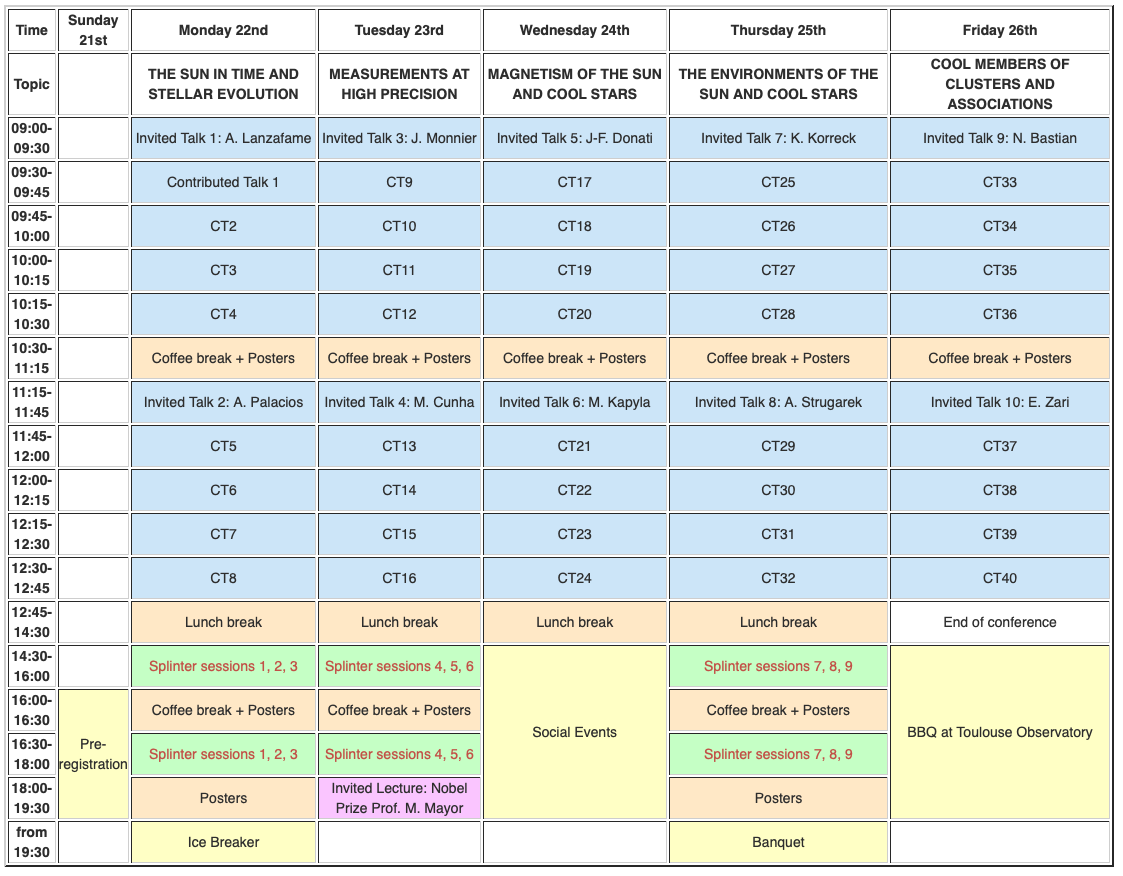
\includegraphics[width=1.15\textheight]{images/schedule.png}
\end{center}

\end{landscape}
% Include information on conference proceedings:
\newpage
\addcontentsline{toc}{chapter}{Instructions for the Conference Proceedings}

\par\noindent{\huge {\bf Instructions for the Conference Proceedings}}
\\
\\
\par\noindent TBD (Zenodo etc.)

\mainmatter


\chapter*{Talks}
\addcontentsline{toc}{chapter}{Talks}
        
          \section[The Missing Members of Nearby Young Associations \newline(Jonathan Gagn\'e)] { The Missing Members of Nearby Young Associations }



%%% ========================
%%% Display authors and their affiliation(s)
%%% ========================
\begin{center}
{\large Jonathan Gagn\'e (1)};{ \large  Eric E. Mamajek (2)};{ \large  Jacqueline K. Faherty (3)};{ \large  Trevor J. David (4)};{ \large  Andrew W. Mann (5)}\\

%%% ===========================================
%%% Show schedule as a margin note for talks, or poster number for posters
%%% ===========================================


\marginnote{ TBA \\ TBA \\  }[0cm]



\index{"Gagn\'e" |textbf }\index{"Mamajek" } \index{"Faherty" } \index{"David" } \index{"Mann" } 
  
\vspace{2 mm}
\noindent (1) Institute for Research on Exoplanets, Université de Montréal; (2)  Jet Propulsion Laboratory, Caltech; (3)  University of North Carolina at Chapel Hill; (4)  American Museum of Natural History\\

\end{center}



%%% ===========
%%% Display abstract
%%% ===========
  
\vspace{2 mm}
\noindent I will present the latest developments in the search for members of young stellar associations in the Solar neighborhood, within 150 pc of the Sun. I will discuss the nature of these sparse and nearby associations and their utility as age-calibrating benchmarks. I will show how the recent Data Release 2 of the ESO Gaia mission is strongly impacting our understanding of the Solar neighborhood, including that of nearby young associations. I will talk about on-going projects to discover new associations entirely, and characterize the low-mass stars of these young associations based on Gaia, down to the brown dwarf mass regime. I will also touch on how near-infrared surveys like 2MASS and WISE allowed us to find a few members down in the regime of giant planet masses.

%%% separation with a double line
\noindent\doubleline
        
          \section[Spectroscopic Characterisation of 90 Southern Cool TESS Candidate Planet Hosts \newline(Adam D. Rains)] { Spectroscopic Characterisation of 90 Southern Cool TESS Candidate Planet Hosts }



%%% ========================
%%% Display authors and their affiliation(s)
%%% ========================
\begin{center}
{\large Adam D. Rains};{ \large  Maruša Žerjal};{ \large  Michael J. Ireland};{ \large  Michael S. Bessell};{ \large  Thomas Nordlander};{ \large  Luca Casagrande}\\

%%% ===========================================
%%% Show schedule as a margin note for talks, or poster number for posters
%%% ===========================================


\marginnote{ TBA \\ TBA \\  }[0cm]



\index{"Rains" |textbf }\index{"Žerjal" } \index{"Ireland" } \index{"Bessell" } \index{"Nordlander" } \index{"Casagrande" } 
  
\vspace{2 mm}
\noindent Australian National University\\

\end{center}



%%% ===========
%%% Display abstract
%%% ===========
  
\vspace{2 mm}
\noindent Cool dwarfs young and old are the most numerous stars in the universe, and are critical to understand due to both this profusion but also to better study the lives of the planets they host. NASA's Transiting Exoplanet Survey Satellite, TESS, has now finished surveying the Southern Hemisphere and has returned a wealth of planet candidates orbiting such stars that are now actively being followed up by ground-based spectroscopic surveys. However, many of these stars are too faint to be effectively targeted by precision radial velocity surveys, leaving host star properties known only through photometry. Here we present the results of a spectroscopic survey of 90 cool (< 4500 K) southern TESS exoplanet candidates in the magnitude range 8.7 < G < 15.8. The stars were observed at medium resolution by the ANU 2.3 m Telescope over a wavelength range 3500-7000 A in late 2019 and early 2020. We derive stellar $T_{\rm eff}$, log g, and [Fe/H] through both synthetic and data driven approaches, and compare the results to empirical relations. Many of our sample had no prior spectroscopic observations, so this work serves to expand our understanding of the coolest stars in Solar Neighbourhood with a uniform set of stellar parameters. Additionally, we compute precision stellar radii for our targets using bolometric fluxes and parallax measurements, enabling us to place radius constraints on the largest sample of TESS planets to date.

%%% separation with a double line
\noindent\doubleline
        
          \section[Magnetic field and activity is M giants - a long term study \newline(Renada Konstantinova-Antova, Agnes Lèbre, Stefan Georgiev, Michel Aurière, Ana Palacios, Julien Morin, Eric Josselin, Natalia Drake, Rumen Bogdanovski, Svetla Tsvetkova, Ana Borisova, Philippe Mathias)] { Magnetic field and activity is M giants - a long term study }



%%% ========================
%%% Display authors and their affiliation(s)
%%% ========================
\begin{center}
{\large Renada Konstantinova-Antova, Agnes Lèbre, Stefan Georgiev, Michel Aurière, Ana Palacios, Julien Morin, Eric Josselin, Natalia Drake, Rumen Bogdanovski, Svetla Tsvetkova, Ana Borisova, Philippe Mathias}\\

%%% ===========================================
%%% Show schedule as a margin note for talks, or poster number for posters
%%% ===========================================


\marginnote{ TBA \\ TBA \\  }[0cm]



\index{"Mathias" |textbf }
  
\vspace{2 mm}
\noindent (1) Institute of Astronomy and NAO, Bulgarian Academy of Sciences; (2)  LUPM, UMR 5299, Université de Montpellier, CNRS; (3)  Institute of Astronomy and NAO, Bulgarian Academy of Sciences; (4)  Université de Toulouse, IRAP; (5)  LUPM, UMR 5299, Université de Montpellier, CNRS; (6)  Laboratory of Observational Astrophysics, Saint Petersburg State University; (7)  Institute of Astronomy and NAO, Bulgarian Academy of Sciences; (8)  Université de Toulouse, IRAP.\\

\end{center}



%%% ===========
%%% Display abstract
%%% ===========
  
\vspace{2 mm}
\noindent A long-term (more than 10 years) spectropolarimetric and spectroscopic study of three magnetic M giants is presented. The Narval spectropolarimeter at the 2m TBL, Pic du Midi Observatory, France, is used for the whole study. The reasons for the  long and short term  variability of the magnetic field and activity  is discussed in the context of the evolutionary stage and the relevant structure of these fairly evolved stars. The interplay between the magnetic field and pulsations is also explored.

%%% separation with a double line
\noindent\doubleline
        
          \section[The Evolution of Stellar Rotation \newline(Jamie Tayar\& the TESS Subgiant Team)] { The Evolution of Stellar Rotation }



%%% ========================
%%% Display authors and their affiliation(s)
%%% ========================
\begin{center}
{\large Jamie Tayar\& the TESS Subgiant Team}\\

%%% ===========================================
%%% Show schedule as a margin note for talks, or poster number for posters
%%% ===========================================


\marginnote{ TBA \\ TBA \\  }[0cm]



\index{"Team" |textbf }
  
\vspace{2 mm}
\noindent Institute for Astronomy/University of Hawaii\\

\end{center}



%%% ===========
%%% Display abstract
%%% ===========
  
\vspace{2 mm}
\noindent Data from Kepler allowed us for the first time to understand the evolution of the internal rotation of evolved stars. These results told a complicated story, where main sequence stars were generally solid body rotators, whereas red giants showed large radial rotation gradients. I will present the first measurements of internal rotation using TESS data for subgiant and lower red giant stars and show that these results allow us to connect these two regimes. I will show that the ratio of the core and envelope rotation in this regime is a function of mass, which helps to explain the previous measurements of core rotation in red giants. I will also demonstrate that these new measurements are a challenge to explain in detail for current theories of internal angular momentum transport and discuss some possibilities for future progress.

%%% separation with a double line
\noindent\doubleline
        
          \section[Realistic Radiative MHD Modeling of Flare-productive Sunspots \newline(Shin Toriumi)] { Realistic Radiative MHD Modeling of Flare-productive Sunspots }



%%% ========================
%%% Display authors and their affiliation(s)
%%% ========================
\begin{center}
{\large Shin Toriumi (1)};{ \large  Hideyuki Hotta (2)}\\

%%% ===========================================
%%% Show schedule as a margin note for talks, or poster number for posters
%%% ===========================================


\marginnote{ TBA \\ TBA \\  }[0cm]



\index{"Toriumi" |textbf }\index{"Hotta" } 
  
\vspace{2 mm}
\noindent (1) Japan Aerospace Exploration Agency; (2)  Chiba University\\

\end{center}



%%% ===========
%%% Display abstract
%%% ===========
  
\vspace{2 mm}
\noindent Observations revealed that the solar flares, especially the strongest events in history, emanate from complex-shaped sunspot regions. However, it has been extremely difficult to investigate the formation of sunspots because we cannot optically observe the subsurface layer of the Sun, where magnetic fields rise and build up sunspots on the photosphere. In this study, for the first time, we succeed in simulating the entire process, in which a subsurface magnetic flux tube is elevated by the turbulent background convection and spontaneously forms complex sunspots. We find that the sunspots have a "delta" configuration (the most eruptive category of sunspots) with a strong magnetic shear and helical flux rope structure, all off which are consistent with the observations of flare-prolific regions. In the presentation, we discuss the key roles of turbulent convection in producing such violent sunspots.

%%% separation with a double line
\noindent\doubleline
        
          \section[Differential rotation and meridional flows on the lower main sequence \newline(Küker, Manfred)] { Differential rotation and meridional flows on the lower main sequence }



%%% ========================
%%% Display authors and their affiliation(s)
%%% ========================
\begin{center}
{\large Küker, Manfred (1)};{ \large  Rüdiger, Günther (2)};{ \large  Strassmeier, Klaus (3)};{ \large  Oláh, Katalin (4)}\\

%%% ===========================================
%%% Show schedule as a margin note for talks, or poster number for posters
%%% ===========================================


\marginnote{ TBA \\ TBA \\  }[0cm]



\index{"Manfred" |textbf }\index{"Günther" } \index{"Klaus" } \index{"Katalin" } 
  
\vspace{2 mm}
\noindent (1) Leibniz-Institut für Astrophysik Potsdam; (2)  Konkoly Observatory Budapest\\

\end{center}



%%% ===========
%%% Display abstract
%%% ===========
  
\vspace{2 mm}
\noindent Mean field models reproduce the observed differential rotation pattern and surface meridional flow of the Sun. Predictions for other stars on the lower main sequence are consistent with observations but raise questions about the validity of the flux transport dynamo as the mechanism behind stellar activity. This is particularly true for early M dwarfs, which show cycle times much shorter than the turnover times predicted by mean field models. 

%%% separation with a double line
\noindent\doubleline
        
          \section[The solar wind angular momentum: what's new with Parker Solar Probe?  \newline(Victor Réville)] { The solar wind angular momentum: what's new with Parker Solar Probe?  }



%%% ========================
%%% Display authors and their affiliation(s)
%%% ========================
\begin{center}
{\large Victor Réville (1)};{ \large  Marco Velli (2)};{ \large  Alexis Rouillard (3)};{ \large  Benoit Lavraud (4)}\\

%%% ===========================================
%%% Show schedule as a margin note for talks, or poster number for posters
%%% ===========================================


\marginnote{ TBA \\ TBA \\  }[0cm]



\index{"Réville" |textbf }\index{"Velli" } \index{"Rouillard" } \index{"Lavraud" } 
  
\vspace{2 mm}
\noindent (1) CNRS/IRAP; (2)  UCLA; (3)  CNRS/IRAP; (4)  CNRS/IRAP\\

\end{center}



%%% ===========
%%% Display abstract
%%% ===========
  
\vspace{2 mm}
\noindent The first few orbits of the Parker Solar Probe have already shaken up our most advanced theories on the solar wind acceleration and angular momentum transport. Non-linear, large amplitude Alfvén waves, called switchbacks, have been observed constantly and may be a fundamental, unexpected, ingredient of the solar wind driving. A surprisingly high co-rotation of the solar wind particles has also been measured at the closest approach of the PSP. This latter observation shatters our hopes to settle the question of the measurement of the solar wind angular momentum once and for all and suggests that something fundamental to the solar and stellar wind braking has yet to be understood. In this talk, I will detail some of the possible explanations for these high azimuthal velocity measurements, such as compression and co-rotating interaction regions, temperature anisotropies and switchback dynamics. I will rely on newly developed simulations of the solar corona and wind as well as simplified analytical calculations. Finally, I will draw some of the potential consequences of these observations on the modeling of cool stars’ rotation evolution on secular timescales. 

%%% separation with a double line
\noindent\doubleline
        
          \section[Can sub-photospheric magnetic reconnection change the elemental composition in the corona? \newline(Baker, Deborah)] { Can sub-photospheric magnetic reconnection change the elemental composition in the corona? }



%%% ========================
%%% Display authors and their affiliation(s)
%%% ========================
\begin{center}
{\large Baker, Deborah (1)};{ \large  van Driel-Gesztelyi, Lidia (2)};{ \large  Brooks, David H. (3)};{ \large  Démoulin, Pascal (4)};{ \large  Valori, Gherardo (5)};{ \large  Long, David M. (6)};{ \large  Laming, J. Martin (7)};{ \large  To, Andy S. H. (8)};{ \large  James, Alexander W. (9)};{ \large  Oláh, Katalin (10)};{ \large  Kővári, Zsolt (11)};{ \large  Green, Lucie M. (12)};{ \large  Matthews, Sarah A.  (13)}\\

%%% ===========================================
%%% Show schedule as a margin note for talks, or poster number for posters
%%% ===========================================


\marginnote{ TBA \\ TBA \\  }[0cm]



\index{"Deborah" |textbf }\index{"Lidia" } \index{"H." } \index{"Pascal" } \index{"Gherardo" } \index{"M." } \index{"Martin" } \index{"H." } \index{"W." } \index{"Katalin" } \index{"Zsolt" } \index{"M." } \index{"A." } 
  
\vspace{2 mm}
\noindent (1) University College London, Mullard Space Science Laboratory; (2)  University College London, Mullard Space Science Laboratory, LESIA, Observatoire de Paris, Université PSL, CNRS, Sorbonne Université, Univ. Paris Diderot, Sorbonne Paris Cité, Konkoly Observatory, Research Centre for Astronomy and Earth Sciences; (3)  College of Science, George Mason University; (4)  LESIA, Observatoire de Paris, Université PSL, CNRS, Sorbonne Université, Univ. Paris Diderot, Sorbonne Paris Cité; (5)  University College London, Mullard Space Science Laboratory; (6)  University College London, Mullard Space Science Laboratory; (7)  Space Science Division, Naval Research Laboratory; (8)  European Space Astronomy Centre; (9)  Konkoly Observatory; (10)  Konkoly Observatory; (11)  University College London, Mullard Space Science Laboratory; (12)  University College London, Mullard Space Science Laboratory\\

\end{center}



%%% ===========
%%% Display abstract
%%% ===========
  
\vspace{2 mm}
\noindent Within the coronae of stars, abundances of those elements with low first ionization potential (FIP) often differ from their photospheric values. The coronae of the Sun and solar-type stars mostly show enhancements of low-FIP elements (the FIP effect) where more active stars such as M-dwarfs have coronae generally characterized by the inverse-FIP effect (I-FIP). Using Hinode/EIS we observe patches of I-FIP effect solar plasma in the midst of FIP-effect plasma in two magnetically complex active regions while magnetic flux is emerging. We argue that the umbrae of coalescing sunspots and more specifically strong light bridges, are preferential locations for observing I-FIP effect plasma. Furthermore, the magnetic complexity of the active region and major episodes of fast flux emergence also lead to repetitive and intense flares. The induced evaporation of the chromospheric plasma in flare ribbons crossing the coalescing umbrae produces high enugh temperatures to enable the observation of localized patches of I-FIP effect plasma in the corona. These observations can be interpreted in the context of the ponderomotive force fractionation model, which predicts that plasma with I-FIP effect composition is created by the refraction of waves coming from below the chromosphere. The refraction takes place in the chromosphere due to a high density gradient there. We propose that the waves generating the I-FIP effect plasma in solar active regions are generated by sub-photospheric (component) reconnection of coalescing flux systems. Although we only glimpse signatures of I-FIP effect fractionation produced by this interaction in patches on the Sun, on highly active M-stars it may be the dominant process.

%%% separation with a double line
\noindent\doubleline
        
          \section[Unraveling the nature of ultra-fast rotators with ASTROSAT \newline(Lalitha Sairam, K.P. Singh, J.H.M.M. Schmitt)] { Unraveling the nature of ultra-fast rotators with ASTROSAT }



%%% ========================
%%% Display authors and their affiliation(s)
%%% ========================
\begin{center}
{\large Lalitha Sairam, K.P. Singh, J.H.M.M. Schmitt}\\

%%% ===========================================
%%% Show schedule as a margin note for talks, or poster number for posters
%%% ===========================================


\marginnote{ TBA \\ TBA \\  }[0cm]



\index{"Schmitt" |textbf }
  
\vspace{2 mm}
\noindent (1) University of Birmingham; (2)  Indian Institute of Science Education and Research Mohali, India; (3)   Hamburger Sternwarte, University of Hamburg\\

\end{center}



%%% ===========
%%% Display abstract
%%% ===========
  
\vspace{2 mm}
\noindent The Sun is often considered to be a prototype of ultra-fast rotating stars.  We often extrapolate the knowledge inferred from the Sun to these stars. However, several studies have shown that the spatial correlation between the different layers of the atmosphere and their associated activity phenomena may or may not be similar to the Sun. Although stellar magnetic activity has been investigated for decades, the exact mechanism controlling the activity of fast-rotating stars are still not understood. We systematically characterise the stellar activity of fast-rotators in the optical, X-ray and UV regime with AstroSat, a multi-wavelength observatory. In this talk, I will invoke how such a multi-wavelength study allows us to localise activity features on the stellar surface and the heating mechanism of the outer layers of the stellar atmosphere. 

%%% separation with a double line
\noindent\doubleline
        
          \section[Surface magnetic field effect on stellar limb darkening. \newline(N. M. Kostogryz)] { Surface magnetic field effect on stellar limb darkening. }



%%% ========================
%%% Display authors and their affiliation(s)
%%% ========================
\begin{center}
{\large N. M. Kostogryz (1)};{ \large  V. Witzke (2)};{ \large   A. I. Shapiro (3)};{ \large  P. F. L. Maxted (4)};{ \large  L. Gizon, S. K. Solanki (5)}\\

%%% ===========================================
%%% Show schedule as a margin note for talks, or poster number for posters
%%% ===========================================


\marginnote{ TBA \\ TBA \\  }[0cm]



\index{"Kostogryz" |textbf }\index{"Witzke" } \index{"Shapiro" } \index{"Maxted" } \index{"Solanki" } 
  
\vspace{2 mm}
\noindent (1) Max Planck Institute for Solar System Research; (2)  Max Planck Institute for Solar System Research; (3)  Max Planck Institute for Solar System Research; (4)  Astrophysics Group at Keele University; (5)  Max Planck Institute for Solar System Research/Institut für Astrophysik, Georg-August-Universität Göttingen; (6)  Max Planck Institute for Solar System Research/School of Space Research at Kyung Hee University\\

\end{center}



%%% ===========
%%% Display abstract
%%% ===========
  
\vspace{2 mm}
\noindent Limb darkening of stellar atmospheres defines the shape of the transit light curve and also affects its depth. Therefore knowledge of the limb darkening is crucial for retrieving parameters of exoplanets  from transit light curves.
We employ the newly developed 1-D MPS-ATLAS code to create a grid of model atmospheres and the corresponding limb darkening for a wide range of stellar fundamental parameters. Moreover, we perform 3-D hydrodynamical (HD) and magnetohydrodynamical (MHD) simulations using the MURaM code for selected combinations of fundamental parameters. 
We show that our 1-D calculations lead to the limb darkening very similar to those returned by the 3D HD MURaM simulations.
At the same time a comparison of HD and MHD 3-D simulations shows that surface magnetic field has a strong effect on the limb darkening functions, and leads to a better agreement with observations.

%%% separation with a double line
\noindent\doubleline
        
          \section[The Sun is less active than other solar-like stars \newline(Timo Reinhold)] { The Sun is less active than other solar-like stars }



%%% ========================
%%% Display authors and their affiliation(s)
%%% ========================
\begin{center}
{\large Timo Reinhold (1)};{ \large  Alexander I. Shapiro (2)};{ \large  Sami K. Solanki (3)};{ \large  Benjamin T. Montet (4)};{ \large  Natalie A. Krivova (5)};{ \large  Robert H. Cameron (6)};{ \large  Eliana M. Amazo-Gomez (7)}\\

%%% ===========================================
%%% Show schedule as a margin note for talks, or poster number for posters
%%% ===========================================


\marginnote{ TBA \\ TBA \\  }[0cm]



\index{"Reinhold" |textbf }\index{"Shapiro" } \index{"Solanki" } \index{"Montet" } \index{"Krivova" } \index{"Cameron" } \index{"Amazo-Gomez" } 
  
\vspace{2 mm}
\noindent (1) Max Planck Institute for Solar System Research (MPS); (2)  MPS; (3)  MPS \& School of Space Research, Kyung Hee University, Yongin, Gyeonggi, 446-701, Korea; (4)  School of Physics, University of New South Wales, Sydney, NSW 2052, Australia; (5)  MPS; (6)  MPS; (7)  MPS \& Georg-August University, Institute for Astrophysics, 37077 Goettingen, Germany\\

\end{center}



%%% ===========
%%% Display abstract
%%% ===========
  
\vspace{2 mm}
\noindent Over the past decades it has been discussed whether the Sun is less active than 
other stars with near-solar effective temperatures and rotation periods. Since 
stellar magnetic activity and photometric variability are strongly correlated, 
we compare the Sun's activity to other solar-like stars. By combining four years 
of photometric observations from the Kepler space telescope with astrometric 
data from the Gaia spacecraft, we measure photometric variabilities of hundrets 
of solar-like stars. Most of the solar-like stars with well-determined rotation 
periods show higher variability than the Sun and are therefore considerably more 
active. These stars appear nearly identical to the Sun, except for the higher 
variability. Their existence raises the question of whether the Sun can also 
experience epochs of such high variability.

%%% separation with a double line
\noindent\doubleline
        
          \section[Magnetic field and accretion in the young eruptive star EX Lupi \newline(Péter Ábrahám)] { Magnetic field and accretion in the young eruptive star EX Lupi }



%%% ========================
%%% Display authors and their affiliation(s)
%%% ========================
\begin{center}
{\large Péter Ábrahám (1)};{ \large  Ágnes Kóspál (2)};{ \large  Andrés Carmona (3)};{ \large  Jean-François Donati (4)};{ \large  Jerôme Bouvier (5)};{ \large  Kundan Kadam (6)};{ \large  Aurora Sicilia-Aguilar (7)};{ \large  Collin Folson (8)}\\

%%% ===========================================
%%% Show schedule as a margin note for talks, or poster number for posters
%%% ===========================================


\marginnote{ TBA \\ TBA \\  }[0cm]



\index{"Ábrahám" |textbf }\index{"Kóspál" } \index{"Carmona" } \index{"Donati" } \index{"Bouvier" } \index{"Kadam" } \index{"Sicilia-Aguilar" } \index{"Folson" } 
  
\vspace{2 mm}
\noindent (1) Konkoly Observatory Budapest; (2)  Konkoly Observatory Budapest, MPIA Heidelberg; (3)  IPAG Grenoble; (4)  IRAP Toulouse; (5)  IPAG Grenoble; (6)  Konkoly Observatory Budapest; (7)  University of Dundee; (8)  IRAP Toulouse\\

\end{center}



%%% ===========
%%% Display abstract
%%% ===========
  
\vspace{2 mm}
\noindent EX Lup is the younger sibling of our Sun. It is a low-mass star with an age of a few million years, which still possesses a strong magnetic field and accretes material actively from its circumstellar disk. According to numerical simulations, the magnetic interaction of the star and its disk may lead to bursts of increased accretion onto the star. An observable example of this phenomenon is EX Lup, which show irregular brightenings due to elevated accretion, giving name to a group of young stars called EXors. EX Lup had its historically largest outburst in 2008. Spectra from its quiescent and outburst periods indicate that the mass accretion proceeds through the same magnetospheric accretion channels in both periods but with different mass flux. Here, we present a study of the magnetic field structure and accretion process in EX Lup. We monitored the star in 2016 June with the CFHT/ESPaDOnS spectropolarimeter and detected strong and largely poloidal topology with a prominent cool polar cap and an accretion spot above it. Our multi-filter optical/near-infrared photometric monitoring between 2016 and 2019 with the SMARTS 1.3m telescope suggests that the location and extent of the spot varied over the years. We also present recent results from our coordinated CFHT/ESPaDOnS and CFHT/SPIRou spectropolarimetric monitoring of EX Lup at the same time as the TESS satellite measured it. If EX Lup is a good proxy for the proto-Sun, similar magnetic field-disk interactions and the resulting outbursts might have happened during the early evolution of the Solar System as well, shaping the formation of the terrestrial planets.

%%% separation with a double line
\noindent\doubleline
        
          \section[The accretion process in the DQ Tau pre-main sequence binary system \newline(Ágnes Kóspál)] { The accretion process in the DQ Tau pre-main sequence binary system }



%%% ========================
%%% Display authors and their affiliation(s)
%%% ========================
\begin{center}
{\large Ágnes Kóspál (1)};{ \large  Evelyne Alecian (2)};{ \large  Péter Ábrahám (3)};{ \large  Jerôme Bouvier (4)};{ \large  Jean-François Donati (5)};{ \large  Andrés Carmona (6)};{ \large  Benjámin Vígh (7)}\\

%%% ===========================================
%%% Show schedule as a margin note for talks, or poster number for posters
%%% ===========================================


\marginnote{ TBA \\ TBA \\  }[0cm]



\index{"Kóspál" |textbf }\index{"Alecian" } \index{"Ábrahám" } \index{"Bouvier" } \index{"Donati" } \index{"Carmona" } \index{"Vígh" } 
  
\vspace{2 mm}
\noindent (1) Konkoly Observatory Budapest, MPIA Heidelberg; (2)  IPAG Grenoble; (3)  Konkoly Observatory Budapest; (4)  IPAG Grenoble; (5)  IRAP Toulouse; (6)  IPAG Grenoble; (7)  Konkoly Observatory Budapest\\

\end{center}



%%% ===========
%%% Display abstract
%%% ===========
  
\vspace{2 mm}
\noindent DQ Tau is a pre-main sequence spectroscopic binary consisting of two M1-type stars on an eccentric orbit surrounded by a circumbinary disk. It's the prototype system for pulsed accretion, a phenomenon during which the binary periodically accretes material from the disk synchronized with the binary's orbital period. DQ Tau is also among the few young stars exhibiting strong, recurrent millimeter flares explained by interaction between the stars' magnetospheres during periastron. Kepler/K2 light curves revealed a rotational modulation by stellar spots with a rotational period of 3.017+/-0.004 days, brief brightening events due to stellar flares, long brightening events around periastron due to increased accretion, and short dips due to brief circumstellar obscuration. Here, we present new VLT/XSHOOTER and CFHT/ESPaDOnS monitoring of DQ Tau. We analyze 8 XSHOOTER spectra taken between 2012 November and 2013 March covering the 300 - 2470 nm wavelength range, and 3 ESPaDOnS spectra taken in 2019 November, covering the 370 - 1050 nm wavelength range. We detect significant variability of the emission line strengths and profiles, as well as of the veiling of the absorption lines over the orbital period of the binary, confirming variable accretion. We discovered forbidden emission lines, indicating the presence of shocked material in the system. Our spectropolarimetric data display clear Zeeman-signature, but the magnetic field in the system is relatively weak. With this project, we aim to further our knowledge on how mass accretion happens in a binary, an important question because many low-mass Sun-like stars are born in multiple systems.

%%% separation with a double line
\noindent\doubleline
        
          \section[What have we learned about Milky Way's young substellar population? \newline(Koraljka Muzic, Aleks Scholz, Victor Almendros-Abad, Karolina Kubiak)] { What have we learned about Milky Way's young substellar population? }



%%% ========================
%%% Display authors and their affiliation(s)
%%% ========================
\begin{center}
{\large Koraljka Muzic, Aleks Scholz, Victor Almendros-Abad, Karolina Kubiak}\\

%%% ===========================================
%%% Show schedule as a margin note for talks, or poster number for posters
%%% ===========================================


\marginnote{ TBA \\ TBA \\  }[0cm]



\index{"Kubiak" |textbf }
  
\vspace{2 mm}
\noindent (1) CENTRA University of Lisbon; (2)  St Andrews University; (3)  CENTRA University of Lisbon; (4)  CENTRA University of Lisbon\\

\end{center}



%%% ===========
%%% Display abstract
%%% ===========
  
\vspace{2 mm}
\noindent Young clusters and star forming regions are home to a large number of substellar objects with masses below the hydrogen-burning limit at $\sim$0.075 M$_\odot$. Most of our knowledge about their populations is coming from nearby regions (d$<$400 pc), where we find consistent formation rates of 2-5 young brown dwarfs per 10 newborn stars. Brown dwarf theories, on the other hand, predict that high gas or stellar densities, as well as the presence of massive OB stars, may be factors that boost the incidence of newly formed brown dwarfs with respect to stars. The next frontier in substellar studies, therefore, is their identification in massive clusters, characterized by drastically different star-forming environments than those found in our immediate vicinity. In this contribution I will compare the outcome of our decade-long deep survey SONYC (Substellar Objects in Nearby Young Clusters), with the results of our new project in massive young clusters, in which we confirm the first bona fide brown dwarfs beyond 1 kpc. I will also discuss the trials and tribulations of membership confirmation in this mass and age regime.

%%% separation with a double line
\noindent\doubleline
        
          \section[Effect of metallicity on small-scale magnetic flux in Sun-like stars \newline(A. I.  Shapiro)] { Effect of metallicity on small-scale magnetic flux in Sun-like stars }



%%% ========================
%%% Display authors and their affiliation(s)
%%% ========================
\begin{center}
{\large A. I.  Shapiro};{ \large   D. Przybylski};{ \large    R. H. Cameron};{ \large   S. K. Solanki};{ \large   N. A. Krivova}\\

%%% ===========================================
%%% Show schedule as a margin note for talks, or poster number for posters
%%% ===========================================


\marginnote{ TBA \\ TBA \\  }[0cm]



\index{"Shapiro" |textbf }\index{"Przybylski" } \index{"Cameron" } \index{"Solanki" } \index{"Krivova" } 
  
\vspace{2 mm}
\noindent Max Planck Institute for Solar System Research,  School of Space Research, Kyung Hee University\\

\end{center}



%%% ===========
%%% Display abstract
%%% ===========
  
\vspace{2 mm}
\noindent Stellar activity is driven by magnetic fields emerging from below the stellar surface and evolving due to the complex interaction of gas dynamics and magnetic flux.  The concentrations of magnetic fields on stellar surfaces form various magnetic features, e.g. faculae.  
Moreover, even when stellar activity is completely absent above a basal level, there is a minimum level of magnetic flux.
This so-called basal flux is due to a local small-scale dynamo (SSD) near the surface. 

Previous investigations of near-surface magneto-convection simulations have demonstrated an important effect of the stellar effective temperature on the underlying physics of stellar magnetic features, finding significant influences on the bolometric intensity, velocity patterns and lifetime of surface magnetic fields.  Another fundamental stellar parameter is metallicity, the effect of which was  mostly ignored in realistic 3D MHD calculations until now. In particular, while extensive studies for several metallicities exist for pure hydrodynamic$\sim$(HD) 3D models, we lack understanding how metallicity will affect magnetic structures.

Here, we focus on the effect of metallicity on stellar near-surface dynamics in the presence of magnetic fields. Using radiative 3D MHD calculations by the \texttt{MURaM} code we simulate Sun-like stars with metallicity values ranging from $\rm M/H = -1.0$ to $\rm M/H = 0.5$. 
To describe the quiet stellar surface, we consider both purely hydrodynamic and SSD runs. To obtain different levels of magnetic activity we use runs with initial vertical magnetic fields of different  strengths. Our study not only investigates the fundamental  properties of near-surface dynamics in solar-like stars of different metallicity, but also  forms the base for numerous applications, such as modelling stellar brightness variability, and determining centre-to-limb variations.

%%% separation with a double line
\noindent\doubleline
        
          \section[Spitzer Mid-IR Monitoring of Young Giant Planet Analogs \newline(Jacqueline Faherty)] { Spitzer Mid-IR Monitoring of Young Giant Planet Analogs }



%%% ========================
%%% Display authors and their affiliation(s)
%%% ========================
\begin{center}
{\large Jacqueline Faherty (1)};{ \large  Kelle Cruz (2)};{ \large  Emily Rice (3)};{ \large  Jonathan Gagn\'e (4)};{ \large  Mark Marley (5)};{ \large  John Gizis (6)}\\

%%% ===========================================
%%% Show schedule as a margin note for talks, or poster number for posters
%%% ===========================================


\marginnote{ TBA \\ TBA \\  }[0cm]



\index{"Faherty" |textbf }\index{"Cruz" } \index{"Rice" } \index{"Gagn\'e" } \index{"Marley" } \index{"Gizis" } 
  
\vspace{2 mm}
\noindent (1) American Museum of Natural History; (2)  American Museum of Natural History; (3)  CUNY, Hunter College; (4)  CUNY, Macaulay Honors College; (5)  University of Montreal; (6)  NASA Ames; (7)  University of Delaware\\

\end{center}



%%% ===========
%%% Display abstract
%%% ===========
  
\vspace{2 mm}
\noindent Photometric variability monitoring is sensitive to atmospheric features as they rotate in and out of view, allowing us to probe the presence of surface inhomogeneities caused by patchy clouds, hot spots and temperature fluctuations. Periodic variability has been detected in brown dwarfs with temperatures spanning 250 - 2200 K, and recently in a sample of free-floating, planetary-mass objects. These young, isolated, low-gravity objects share a striking resemblance with the directly-imaged planets and can be studied in far greater detail in the absence of a bright host star. The large amplitudes observed in this small sample of low-gravity objects suggests that variability may be enhanced for the exoplanet analogues. I will present results from a large Spitzer survey searching for variability in young, giant planet analogs, and discuss how these results reveal how the temperature, surface-gravity, rotation rate and inclination can influence observed variability properties.

%%% separation with a double line
\noindent\doubleline
        
          \section[Global Solar Magnetic Variations using Spectroscopic Proxies and Excess Brightness Indices \newline(Ekaterina Dineva)] { Global Solar Magnetic Variations using Spectroscopic Proxies and Excess Brightness Indices }



%%% ========================
%%% Display authors and their affiliation(s)
%%% ========================
\begin{center}
{\large  Ekaterina Dineva (1)};{ \large  Jeniveve Pearson (2)};{ \large  Meetu Verma (3)};{ \large  Carsten Denker (4)};{ \large  Klaus G. Strassmeier (5)};{ \large  Ilya Ilyin (6)}\\

%%% ===========================================
%%% Show schedule as a margin note for talks, or poster number for posters
%%% ===========================================


\marginnote{ TBA \\ TBA \\  }[0cm]



\index{"Dineva" |textbf }\index{"Pearson" } \index{"Verma" } \index{"Denker" } \index{"Strassmeier" } \index{"Ilyin" } 
  
\vspace{2 mm}
\noindent (1) Leibniz Institute for Astrophysics Potsdam (AIP)/ University of Potsdam; (2)  Ohio State University; (3)  Leibniz Institute for Astrophysics Potsdam (AIP); (4)  Leibniz Institute for Astrophysics Potsdam (AIP); (5)  Leibniz Institute for Astrophysics Potsdam (AIP)/ University of Potsdam; (6)  Leibniz Institute for Astrophysics Potsdam (AIP)\\

\end{center}



%%% ===========
%%% Display abstract
%%% ===========
  
\vspace{2 mm}
\noindent The Potsdam Echelle Polarimetric and Spectroscopic Instrument (PEPSI) is a state-of-the-art, thermally stabilized, fiber-fed, high-resolution spectrograph for the Large Binocular Telescope (LBT) at Mt.\ Graham, Arizona. It can be fed with sunlight from the Solar Disk-Integrated (SDI) telescope. Synoptic solar observations with PEPSI/SDI produce daily spectra with high signal-to-noise ratio, providing access to unprecedented, quasi-continuous, long-term, disk-integrated spectra of the Sun with high spectral and temporal resolution. The observed spectra contain a multitude of photospheric and chromospheric spectral lines in the wavelength range of 380\,--\,910$\sim$nm. Strong chromospheric absorption lines, such as the Ca\,\textsc{ii}\,H\,\&\,K lines, are powerful diagnostic tools for solar activity studies, since they trace the variations of the solar magnetic field. Derivation of activity indices, such as the Ca\,\textsc{ii}\,H\,\&\,K emission ratio $S$-index provides insight into the chromospheric magnetic field and its variability over the solar activity cycle. The well known relation between solar calcium indices and UV flux variations motivates us to compute an excess brightness indices from Ca\,\textsc{ii}\,K full-disk images from of the Chromospheric Telescope (ChroTel) at the Observatory del Teide on Tenerife, Spain and UV data of the  Solar Dynamics Observatory (SDO). We present a set of indices representing magnetic activity at various heights in the solar atmosphere. In the present work, we carefully compare the indices computed from various datasets and discuss the differences in terms of physical and observational properties.

%%% separation with a double line
\noindent\doubleline
        
          \section[Disks and outflows of FUor-type stars observed with ALMA \newline(Ágnes Kóspal)] { Disks and outflows of FUor-type stars observed with ALMA }



%%% ========================
%%% Display authors and their affiliation(s)
%%% ========================
\begin{center}
{\large Ágnes Kóspal (1)};{ \large  Péter Ábrahám (2)};{ \large  Michihiro Takami (3)}\\

%%% ===========================================
%%% Show schedule as a margin note for talks, or poster number for posters
%%% ===========================================


\marginnote{ TBA \\ TBA \\  }[0cm]



\index{"Kóspal" |textbf }\index{"Ábrahám" } \index{"Takami" } 
  
\vspace{2 mm}
\noindent (1) Konkoly Observatory \& Max Planck Institute for Astronomy; (2)  Konkoly Observatory; (3)  Institute of Astronomy and Astrophysics, Academia Sinica\\

\end{center}



%%% ===========
%%% Display abstract
%%% ===========
  
\vspace{2 mm}
\noindent FU Orionis-type stars (FUors) are low-mass young stellar objects experiencing brief periods of an enhanced mass accretion rate. The episodic nature of the accretion outbursts has been proposed as a solution for the ``luminosity problem'' where protostars are less luminous that theoretically expected. Previous observations of these objects have shown the compact nature of their protoplanetary disks and, in some cases, massive outflows emanating from them have been observed with different gas tracers. In this work we present the results of our ALMA survey in which we observed 10 different FUor-like objects using the 1.33 mm continuum and the J=2--1 transitions of $^{12}$CO, $^{13}$CO and C$^{18}$O. Our observations consist of two ALMA extended configurations supported by ACA and single dish data. This setup provides us with high angular resolution ($\sim$18 mas) while preserving the short spacing information. As part of our results in the continuum, we analyzed the observed visibilities to determine the disk sizes and masses. In the CO, we recovered outflow emission from several of our targets, and found indications of Keplerian rotation and infalling material. We will also present our serendipitous detection of complex organic molecules and sulfur based molecules. Finally, we will put our sample into context by comparing it to quiescent and other outbursting protostars.

%%% separation with a double line
\noindent\doubleline
        
          \section[Magnetic Variability of Ultracool Dwarfs from TESS \newline(Sarah J. Schmidt)] { Magnetic Variability of Ultracool Dwarfs from TESS }



%%% ========================
%%% Display authors and their affiliation(s)
%%% ========================
\begin{center}
{\large Sarah J. Schmidt (1)};{ \large  Ekaterina Ilin (2)};{ \large  J. Sebastian Pineda (3)};{ \large  Elisabeth R. Newton (4)};{ \large  James R. A. Davenport (5)};{ \large  Adam J. Burgasser (6)}\\

%%% ===========================================
%%% Show schedule as a margin note for talks, or poster number for posters
%%% ===========================================


\marginnote{ TBA \\ TBA \\  }[0cm]



\index{"Schmidt" |textbf }\index{"Ilin" } \index{"Pineda" } \index{"Newton" } \index{"Davenport" } \index{"Burgasser" } 
  
\vspace{2 mm}
\noindent (1) Leibniz Institute for Astrophysics - Potsdam (AIP); (2)  Leibniz Institute for Astrophysics - Potsdam (AIP); (3)  University of Colorado; (4)  Dartmouth College; (5)  University of Washington; (6)  University of California San Diego\\

\end{center}



%%% ===========
%%% Display abstract
%%% ===========
  
\vspace{2 mm}
\noindent Ultracool dwarfs (spectral types M6-L3) encompass both the lowest mass stars and warmest brown dwarfs. Fast rotation periods and strong magnetic fields persist to older ages than for main sequence stars so that most ultracool dwarfs are intrinsically variable. Their magnetic activity gives rise to surface spots and dramatic flares. This activity has been traced by a number of different indicators such as radio, x-ray, and H$\alpha$ emission. The presence and frequency of flares provides a magnetic tracer that is sensitive to changes in spectral type, rotation, and age in most partly und fully convective stars. Data from time domain surveys provides the unique opportunity to study both rotation periods and flares for increasingly large samples of stars. We initiated a program to examine ultracool dwarf rotational and flaring variability using NASA's Transiting Exoplanet Survey Satellite (TESS) two-minute cadence data. We present initial stellar properties, rotation periods, and flare frequency distributions for over one hundred ultracool dwarfs observed with TESS. In our initial results, we find that ultracool dwarfs flare more frequently than expected based on previous studies, but the flare rate does not depend strongly on spectral type.

%%% separation with a double line
\noindent\doubleline
        
          \section[Open Cluster Surveys Reveal a Temporary Epoch of Stalled Spin-Down \newline(Jason Lee Curtis)] { Open Cluster Surveys Reveal a Temporary Epoch of Stalled Spin-Down }



%%% ========================
%%% Display authors and their affiliation(s)
%%% ========================
\begin{center}
{\large Jason Lee Curtis}\\

%%% ===========================================
%%% Show schedule as a margin note for talks, or poster number for posters
%%% ===========================================


\marginnote{ TBA \\ TBA \\  }[0cm]



\index{"Curtis" |textbf }
  
\vspace{2 mm}
\noindent American Museum of Natural History\\

\end{center}



%%% ===========
%%% Display abstract
%%% ===========
  
\vspace{2 mm}
\noindent Recent measurements of stellar rotation periods in benchmark open clusters demonstrate that, after converging onto a tight sequence of slowly rotating stars in mass-period space, stars temporarily stop spinning down. These data also show that the duration of this epoch of stalled spin-down increases toward lower masses. To determine when stalled stars resume spinning down, we used ground- and space-based time series imaging data (e.g., Kepler, K2, TESS, PTF, ZTF) to measure rotation periods for low-mass members of four old open clusters: NGC 6811 (1.0 Gyr), NGC 752 (1.4 Gyr), Ruprecht 147 (2.7 Gyr), and M67 (4 Gyr). The sequence of slowly rotating stars for Ruprecht 147 appears relatively flat, in sharp contrast with the steep mass dependence seen in the younger clusters, where periods tend to get longer toward decreasing mass. We suggest that this flat sequence is produced by the mass-dependent duration of the epoch of stalled braking: while the higher-mass stars spin more rapidly than lower-mass stars at the age of Praesepe (700 Myr), they resume spinning down earlier, and so catch up to their lower-mass siblings just as these resume spinning down. We calculate the time at which stars resume spinning down, and find that 0.55 $M_\odot$ stars remain stalled for at least 1.3 Gyr. The steep mass dependence also means that this phenomenon might present a big obstacle for age-dating stars of even lower mass with rotation. To accurately age-date low-mass stars in the field, gyrochronology formulae must be modified to account for this stalling timescale. Empirically tuning a core-envelope coupling model with open cluster data can account for most of the apparent stalling effect. However, alternative explanations, e.g., a temporary reduction in the magnetic braking torque, cannot yet be ruled out.

%%% separation with a double line
\noindent\doubleline
        
          \section[Tracking density variations in the Solar corona \newline(Léa Griton, Alexis P. Rouillard)] { Tracking density variations in the Solar corona }



%%% ========================
%%% Display authors and their affiliation(s)
%%% ========================
\begin{center}
{\large  Léa Griton, Alexis P. Rouillard (1)};{ \large  Rui Pinto (2)};{ \large  Athanasios Kouloumvakos (3)};{ \large  Nicolas Poirier (4)};{ \large  Michaël
Lavarra (5)};{ \large  Victor Réville (6)};{ \large  Benoît Lavraud (7)};{ \large  Marco Velli (8)};{ \large  Nour-Eddine Raouafi (9)}\\

%%% ===========================================
%%% Show schedule as a margin note for talks, or poster number for posters
%%% ===========================================


\marginnote{ TBA \\ TBA \\  }[0cm]



\index{"Rouillard" |textbf }\index{"Pinto" } \index{"Kouloumvakos" } \index{"Poirier" } \index{"Lavarra" } \index{"Réville" } \index{"Lavraud" } \index{"Velli" } \index{"Raouafi" } 
  
\vspace{2 mm}
\noindent (1) IRAP, Université de Toulouse, CNRS, CNES, UPS, (Toulouse), France ; (2)  IRAP, Université de Toulouse, CNRS, CNES, UPS, (Toulouse), France ; (3)  IRAP, Université de Toulouse, CNRS, CNES, UPS, (Toulouse), France ; (4)  IRAP, Université de Toulouse, CNRS, CNES, UPS, (Toulouse), France ; (5)  IRAP, Université de Toulouse, CNRS, CNES, UPS, (Toulouse), France ; (6)  IRAP, Université de Toulouse, CNRS, CNES, UPS, (Toulouse), France; (7) IRAP, Université de Toulouse, CNRS, CNES, UPS, (Toulouse), France ; (8)  IRAP, Université de Toulouse, CNRS, CNES, UPS, (Toulouse), France ; (9)  Institute of Geophysics \& Planetary Physics, Department of Earth, Planetary \& Space Sciences, University of California, Los Angeles, CA, USA) ; (10)  Johns Hopkins University, Applied Physics Laboratory, Laurel, MD, USA \\

\end{center}



%%% ===========
%%% Display abstract
%%% ===========
  
\vspace{2 mm}
\noindent The recent analysis of Parker Solar Probe's (PSP's) second encounter compared with data taken by the Solar and Heliospheric Observatory (SOHO) and Solar TErrestrial RElations Observatory (STEREO) A (STA) revealed for the first time a close link between the high-density plasma measured by PSP and streamer flows imaged by instruments at 1$\sim$AU from the Sun. We exploit observations when STA was in orbital quadrature with PSP to track the release and propagation of dense material from the corona to PSP. The analysis of time-elongation maps, built from STA images, show that PSP was impacted continually by the southern edge of streamer transients inducing clear density increases measured in situ by the plasma instrument. Considering PSP’s first and second encounters, we also find evidence that the impact of specific dense structures is correlated with a higher occurrence of magnetic field reversals. These magnetic reversals are associated with strong density variations when associated with streamer flows, but with weak density variations outside streamer flows. We present a detailed analysis of the properties of switchbacks in these different slow flows. We compare the magnetic and speed components as well as the correlation between speed and density. This work was funded by the European Research Council through the project SLOW$\_$SOURCE - DLV-819189.

%%% separation with a double line
\noindent\doubleline
        
          \section[Modelling the link between UV emission and stellar magnetic activity \newline(Sowmya Krishnamurthy)] { Modelling the link between UV emission and stellar magnetic activity }



%%% ========================
%%% Display authors and their affiliation(s)
%%% ========================
\begin{center}
{\large Sowmya Krishnamurthy(1) (1)};{ \large  Alexander I. Shapiro(1) (2)};{ \large  Veronika Witzke(1) (3)};{ \large  Nina-Elisabeth Nemec(1) (4)};{ \large  Theodosios Chatzistergos(2) (5)};{ \large  Natalie A. Krivova(1) (6)};{ \large  Sami K. Solanki(1,3) (7)}\\

%%% ===========================================
%%% Show schedule as a margin note for talks, or poster number for posters
%%% ===========================================


\marginnote{ TBA \\ TBA \\  }[0cm]



\index{"Krishnamurthy(1)" |textbf }\index{"Shapiro(1)" } \index{"Witzke(1)" } \index{"Nemec(1)" } \index{"Chatzistergos(2)" } \index{"Krivova(1)" } \index{"Solanki(1,3)" } 
  
\vspace{2 mm}
\noindent (1) (1)Max-Planck-Institut f\"ur Sonnensystemforschung,
Justus-von-Liebig-Weg 3, 37077 G\"ottingen, Germany; (2)  (2)INAF Osservatorio Astronomico di Roma, Via Frascati 33,
00078 Monte Porzio Catone, Italy; (3)  (3)School of Space Research, Kyung Hee University,
YongIn, Gyeonggi 446--701, Korea\\

\end{center}



%%% ===========
%%% Display abstract
%%% ===========
  
\vspace{2 mm}
\noindent The emission in the near ultraviolet Ca$\,{\sc ii}$ H \& K lines
is modulated by the magnetic activity of a star. Although
this emission has been serving as a prime proxy
of magnetic activity for several decades, many aspects
of the complex relation between stellar magnetism and
Ca$\,{\sc ii}$ H \& K  emission are still unclear. In particular,
it was suspected that  Ca$\,{\sc ii}$ H \& K emission might be
also affected by the inclination of a star's rotation axis and
stellar metallicity but until now these effects have remained largely
unexplored. In order to fill in this gap we develop a
physics-based model of Ca$\,{\sc ii}$ H \& K emission which enables
us to study such dependencies. We first test this model for the
case of the Sun, making use of the distributions of the solar
magnetic features derived from observations together with the
Ca$\,{\sc ii}$ spectra synthesized with a non-LTE radiative transfer
code. Its performance is validated by successfully reconstructing
the observed variations of Ca$\,{\sc ii}$ emission across four solar
activity cycles. We then use our model to obtain a time-series of
the Ca$\,{\sc ii}$ emission over a period of 300 years in the past.
With the help of this time-series we investigate the effects of stellar
inclination and metallicity. In particular, we find that for solar-like
distribution of magnetic features, during the cycle maximum,
the Ca$\,{\sc ii}$ emission increases gradually as the angle between
the direction to the observer and stellar rotation axis increases,
while we see an opposite trend for the cycle minimum. Our work allows
us to better understand the intricate coupling between the stellar
parameters and Ca$\,{\sc ii}$ emission, thus enhancing the diagnostic
potential of these emission measurements.

%%% separation with a double line
\noindent\doubleline
        
          \section[Investigating the Atmospheric Compositions of Ultra-Cool Brown Dwarfs Using High Resolution Spectroscopy \newline(Nicole Wallack)] { Investigating the Atmospheric Compositions of Ultra-Cool Brown Dwarfs Using High Resolution Spectroscopy }



%%% ========================
%%% Display authors and their affiliation(s)
%%% ========================
\begin{center}
{\large Nicole Wallack (1)};{ \large  Heather Knutson (2)};{ \large  Marta Bryan (3)};{ \large  Caroline Morley (4)};{ \large  Geoffrey Blake (5)};{ \large  Brendan Bowler (6)};{ \large  Courtney Dressing (7)};{ \large  Emily Martin (8)};{ \large  Andrew Skemer (9)}\\

%%% ===========================================
%%% Show schedule as a margin note for talks, or poster number for posters
%%% ===========================================


\marginnote{ TBA \\ TBA \\  }[0cm]



\index{"Wallack" |textbf }\index{"Knutson" } \index{"Bryan" } \index{"Morley" } \index{"Blake" } \index{"Bowler" } \index{"Dressing" } \index{"Martin" } \index{"Skemer" } 
  
\vspace{2 mm}
\noindent (1) Caltech; (2)  Caltech; (3)  UC Berkeley; (4)  The University of Texas at Austin; (5)  Caltech; (6)  The University of Texas at Austin; (7)  UC Berkeley; (8)  UC Santa Cruz; (9)  UC Santa Cruz\\

\end{center}



%%% ===========
%%% Display abstract
%%% ===========
  
\vspace{2 mm}
\noindent Ultra-cool brown dwarfs serve as an important link between gas giant exoplanets and stars. These objects are expected to have atmospheric chemistries similar to those of cool (<1000 K) transiting gas giant planets, and therefore serve as an important testing ground for atmosphere models. Although we can detect thermal emission from cool transiting gas giant exoplanets by observing secondary eclipses with the Spitzer Space Telescope, we must rely on forward models to interpret these relatively low SNR photometric data.  Isolated or wide separation ultra-cool brown dwarfs, on the other hand, can be observed at both higher resolution and higher SNR using ground based facilities such as the recently upgraded NIRSPEC instrument on Keck. These observations provide an invaluable opportunity to evaluate the accuracy of the models used to interpret exoplanet spectra in this temperature regime. In this study we obtain high-resolution (R$\sim$25,000) K band spectra for two ultra-cool brown dwarfs with temperatures of 500 and 700 K, and detect absorption from methane, ammonia, and water.  We combine these data with previously published low and medium resolution observations of these objects in order to derive updated constraints on their effective temperatures, surface gravities, and metallicities using a machine learning retrieval method leveraging the recently published Sonora model grid (Fisher et al. 2019, Marley et al. in prep). We also use these same data to explore possible modifications to the models that have the potential to improve the overall quality of the fit.

%%% separation with a double line
\noindent\doubleline
        
          \section[Activity-related Oscillation Mode Frequency Shifts from the Main Sequence to the AGB - Theory, Measurement, Implications \newline(René Kiefer)] { Activity-related Oscillation Mode Frequency Shifts from the Main Sequence to the AGB - Theory, Measurement, Implications }



%%% ========================
%%% Display authors and their affiliation(s)
%%% ========================
\begin{center}
{\large René Kiefer};{ \large  Anne-Marie Broomhall}\\

%%% ===========================================
%%% Show schedule as a margin note for talks, or poster number for posters
%%% ===========================================


\marginnote{ TBA \\ TBA \\  }[0cm]



\index{"Kiefer" |textbf }\index{"Broomhall" } 
  
\vspace{2 mm}
\noindent University of Warwick, Centre for Fusion, Space and Astrophysics, Coventry, UK\\

\end{center}



%%% ===========
%%% Display abstract
%%% ===========
  
\vspace{2 mm}
\noindent The properties of stellar oscillation eigenmodes change with the level of magnetic activity.  This has been measured with data from CoRoT and \textit{Kepler}, where signatures of magnetic activity have been found in the seismic properties of a few dozen main-sequence and sub-giant stars. However, as of yet, no detection of temporal variations in the oscillation frequencies of more evolved stars have been reported. 

\textbf{Theory:} To gauge the sensitivity of p modes to magnetic perturbations through stellar evolution, we calculate the mode sensitivity factors of radial p modes for a set of MESA models with initial masses between 0.7--3.0\,$M_{\odot}$ from the main sequence to the early asymptotic giant branch. The mode eigenfunctions are calculated with GYRE. We fit these mode sensitivities with polynomials in fundamental stellar parameters and find that the best-fitting relations differ from those proposed in the literature and that they change between stages of stellar evolution.

\textbf{Measurements:} We analyse the \textit{Kepler} long cadence data for the red giant sample compiled by Yu et al. (2018, ApJS 236:42) which consists of $\sim$16,000 stars. To expand the sample, we added 415 main-sequence and subgiant stars investigated by Serenelli et al. (APOKASC, 2017, ApJS 233:23) and the previously published frequency shifts for a sample of 87 main-sequence and subgiant stars of Santos et al. (2018, ApJS 237:17). To obtain the frequency shifts, we use a cross-correlation technique which is well suited for such a large sample of stars, as the only required input parameters are frequency of maximum oscillation amplitude $\nu_{\text{max}}$ and the large frequency separation $\Delta\nu$. 

We find significant frequency shifts for about 2500 stars of the red giant sample and for 90 stars of the APOKASC sample. Interestingly, stars in the core helium burning phase (as identified by Yu et al.) show larger shifts than stars on the red giant branch. 
\textbf{Implications}: Together with a measure of the strength of the level of magnetic activity, the polynomial scaling relations for the mode sensitivities can be used for assessing whether a star's observed oscillation frequencies are likely to be close to the unperturbed ground state or whether they should be adjusted. This can be important if individual mode frequencies are used for stellar modelling or if $\nu_{\text{max}}$ and $\Delta\nu$ are used to estimate stellar masses and radii. We compare the detected frequency shifts with predictions from our theoretical scaling relations. Further, we discuss implications of the found levels of frequency perturbations and possible means to obtain the “ground state” frequencies.

%%% separation with a double line
\noindent\doubleline
        
          \section[Surface magnetic field effect on stellar limb darkening. \newline(N. M. Kostogryz)] { Surface magnetic field effect on stellar limb darkening. }



%%% ========================
%%% Display authors and their affiliation(s)
%%% ========================
\begin{center}
{\large N. M. Kostogryz (1)};{ \large  V. Witzke (2)};{ \large   A. I. Shapiro (3)};{ \large  P. F. L. Maxted (4)};{ \large  L. Gizon, S. K. Solanki (5)}\\

%%% ===========================================
%%% Show schedule as a margin note for talks, or poster number for posters
%%% ===========================================


\marginnote{ TBA \\ TBA \\  }[0cm]



\index{"Kostogryz" |textbf }\index{"Witzke" } \index{"Shapiro" } \index{"Maxted" } \index{"Solanki" } 
  
\vspace{2 mm}
\noindent (1) Max Planck Institute for Solar System Research; (2)  Max Planck Institute for Solar System Research; (3)  Max Planck Institute for Solar System Research; (4)  Astrophysics Group at Keele University; (5)  Max Planck Institute for Solar System Research/Institut für Astrophysik, Georg-August-Universität Göttingen; (6)  Max Planck Institute for Solar System Research/School of Space Research at Kyung Hee University\\

\end{center}



%%% ===========
%%% Display abstract
%%% ===========
  
\vspace{2 mm}
\noindent Limb darkening of stellar atmospheres defines the shape of the transit light curve and also affects its depth. Therefore knowledge of the limb darkening is crucial for retrieving parameters of exoplanets  from transit light curves.
We employ the newly developed 1-D MPS-ATLAS code to create a grid of model atmospheres and the corresponding limb darkening for a wide range of stellar fundamental parameters. Moreover, we perform 3-D hydrodynamical (HD) and magnetohydrodynamical (MHD) simulations using the MURaM code for selected combinations of fundamental parameters. 
We show that our 1-D calculations lead to the limb darkening very similar to those returned by the 3D HD MURaM simulations.
At the same time a comparison of HD and MHD 3-D simulations shows that surface magnetic field has a strong effect on the limb darkening functions, and leads to a better agreement with observations.

%%% separation with a double line
\noindent\doubleline
        
          \section[Probing fossil magnetism effects in the core of evolved low-mass stars using mixed-mode frequencies \newline(Lisa Bugnet)] { Probing fossil magnetism effects in the core of evolved low-mass stars using mixed-mode frequencies }



%%% ========================
%%% Display authors and their affiliation(s)
%%% ========================
\begin{center}
{\large Lisa Bugnet (1)};{ \large  Vincent Prat (2)};{ \large  Stéphane Mathis (3)};{ \large  Rafael A. García (4)};{ \large  Savita Mathur (5)};{ \large  Kyle Augustson (6)};{ \large  Coralie Neiner (7)}\\

%%% ===========================================
%%% Show schedule as a margin note for talks, or poster number for posters
%%% ===========================================


\marginnote{ TBA \\ TBA \\  }[0cm]



\index{"Bugnet" |textbf }\index{"Prat" } \index{"Mathis" } \index{"García" } \index{"Mathur" } \index{"Augustson" } \index{"Neiner" } 
  
\vspace{2 mm}
\noindent (1) AIM, CEA, CNRS, Université Paris-Saclay, Université Paris Diderot, Sorbonne Paris Cité, F-91191 Gif-sur-Yvette, France; (2)  
AIM, CEA, CNRS, Université Paris-Saclay, Université Paris Diderot, Sorbonne Paris Cité, F-91191 Gif-sur-Yvette, France; (3)  
AIM, CEA, CNRS, Université Paris-Saclay, Université Paris Diderot, Sorbonne Paris Cité, F-91191 Gif-sur-Yvette, France; (4) 
AIM, CEA, CNRS, Université Paris-Saclay, Université Paris Diderot, Sorbonne Paris Cité, F-91191 Gif-sur-Yvette, France; (5) 
Instituto de Astrofisica de Canarias, E-38200, La Laguna, Tenerife, Spain; (6) 
AIM, CEA, CNRS, Université Paris-Saclay, Université Paris Diderot, Sorbonne Paris Cité, F-91191 Gif-sur-Yvette, France; (7) 
LESIA, Paris Observatory, CNRS, PSL University, Sorbonne Université, Univ. Paris Diderot, Sorbonne Paris Cité, 5 place Jules Janssen, 92195 Meudon, France\\

\end{center}



%%% ===========
%%% Display abstract
%%% ===========
  
\vspace{2 mm}
\noindent From the flat rotation profile of the inner Sun to the interestingly low rotation rate of the core of red giants, which is about 10 times lower than what is predicted by the current theory of dynamical processes, the stellar angular momentum transport is poorly understood inside low-mass solar-like stars all along their evolution. The recent discovery of red giants more massive than $\sim1.3$ $M_\odot$ that present a surprisingly low amplitude of the mixed (i.e. modes that behave as acoustic modes in the external envelope and as gravity modes in the core of evolved stars) dipolar and quadrupolar modes could be the signature of a strong magnetic field trapped inside the radiative interior of intermediate mass stars. Regarding the presence of highly magnetised white dwarfs, we seek a missing process taking place inside the core of evolved low-mass stars to efficiently transport angular momentum from the core to the surface. Such a process could arise from strong internal magnetism.
In this context, the mixed modes observed thanks to CoRoT, Kepler/K2 and TESS space missions can constitute an excellent probe of the deepest layers in evolved stars. Stars more massive than $\sim1.3$ $M_\odot$ are known to develop a convective core during the main-sequence: the dynamo process due to this convection could be the origin of a strong magnetic field, trapped inside the core of the star for the rest of its evolution. Such magnetic fields should impact the mixed modes inside the core of RG stars, and their signature should be visible in asteroseismic data. To unravel which constraints can be obtained from these asteroseismic observations, we theoretically investigate the effects of a plausible mixed magnetic field with various amplitudes on the mixed-mode frequencies for subgiant and red giant stars. Applying a perturbative method along with an order-of-magnitude analysis, we estimate the magnetic perturbation on the frequencies of mixed dipolar modes, depending on the magnetic field strength and its configuration. It is then possible to infer an upper limit for the strength of the field and the associated lower limit for the timescales of its action to redistribute angular momentum in stellar interiors.

%%% separation with a double line
\noindent\doubleline
        
          \section[Complex Structure of a Proto-Brown Dwarf \newline(B. Riaz, M. N. Machida)] { Complex Structure of a Proto-Brown Dwarf }



%%% ========================
%%% Display authors and their affiliation(s)
%%% ========================
\begin{center}
{\large B. Riaz, M. N. Machida}\\

%%% ===========================================
%%% Show schedule as a margin note for talks, or poster number for posters
%%% ===========================================


\marginnote{ TBA \\ TBA \\  }[0cm]



\index{"Machida" |textbf }
  
\vspace{2 mm}
\noindent (1) Universitats-Sternwarte Munchen, Ludwig-Maximilians-Universitat, Scheinerstr. 1, 81679 Munchen, Germany; (2)  Department of Earth and Planetary Sciences, Faculty of Sciences, Kyushu University, Fukuoka, Japan\\

\end{center}



%%% ===========
%%% Display abstract
%%% ===========
  
\vspace{2 mm}
\noindent We present ALMA 12CO (2-1), 13CO (2-1), C18O (2-1) molecular line observations of a very young proto-brown dwarf (proto-BD) system in its early formation stages. We have conducted physical-chemical modelling of the complex internal structure for this proto-BD system using the physical structure from the core collapse simulations for brown dwarf formation at different evolutionary stages. We have shown that the model at a stage of $\sim$6000 yr can provide a good fit to the 12CO (2-1), 13CO (2-1), and C18O spectra and reproduce the complex structures seen in the observed integrated intensity maps. Results from modelling the observed morphology and kinematics indicate that 12CO emission is tracing an extended ($\sim$1000 au) molecular outflow, 13CO is tracing the outer ($\sim$1000 au) envelope/pseudo-disk regions, and C18O and 1.3 mm continuum emission are tracing the inner ($\sim$500 au) pseudo-disk. 
In addition, we have observed the 10 $\mu$m silicate absorption spectrum for the proto-BD, which is indicative of crystalline enstatite and forsterite silicates. Crystallization was likely expedited in this system due to strong jet/outflow activity. 
We have built a 3D physical model to interpret the complex internal structure of the proto-BD. This proto-BD system is viewed through a wide outflow cavity, due to which the embedded core is hidden and the envelope/pseudo-disk regions are partially visible, while giving a direct view of the jet/outflow. The various signatures of the proto-BD system, in particular, the very young $\sim$616 yr outflow dynamical age, the high outflow rate of the order of 10-7 Msun/yr, and the comparable envelope and outflow sizes, are indicative of an early Class 0 stage system being formed via the mechanism of gravitational collapse of a very low-mass core.

%%% separation with a double line
\noindent\doubleline
        
          \section[The chemical composition of stars and their rotational evolution \newline(Louis Amard)] { The chemical composition of stars and their rotational evolution }



%%% ========================
%%% Display authors and their affiliation(s)
%%% ========================
\begin{center}
{\large Louis Amard (1)};{ \large  Julia M. T. Roquette (2)};{ \large  Sean Matt (3)}\\

%%% ===========================================
%%% Show schedule as a margin note for talks, or poster number for posters
%%% ===========================================


\marginnote{ TBA \\ TBA \\  }[0cm]



\index{"Amard" |textbf }\index{"Roquette" } \index{"Matt" } 
  
\vspace{2 mm}
\noindent (1) University of Exeter; (2)  University of Exeter; (3)  University of Exeter\\

\end{center}



%%% ===========
%%% Display abstract
%%% ===========
  
\vspace{2 mm}
\noindent The spin-down of stars with time can be used as a tool to provide stellar ages under certain conditions. Large photometric surveys such as Kepler, TESS or even GAIA, thus relies on rotation period measurement to estimate the age of cool main sequence stars. 
However, this gyrochronology technique has so far been well tested and calibrated mostly on young stars of solar metallicity, while field stars are mostly relatively old and cover a broad range of chemical compositions.
In this talk I will review the recent works on rotational evolution models of cool main-sequence stars, their chemical composition, and the consequences on age determination via gyrochronology. 
As an example, I will present a direct application of recent models on the Kepler field. I will finally discuss the direction on which progress towards a global stellar rotation model can be made and its role to play in the interpretation of future surveys.

%%% separation with a double line
\noindent\doubleline
        
          \section[Are the rotation period distributions in zero-age main sequence open clusters alike? \newline(Dario J. Fritzewski, Sydney A. Barnes, David J. James, Klaus G. Strassmeier)] { Are the rotation period distributions in zero-age main sequence open clusters alike? }



%%% ========================
%%% Display authors and their affiliation(s)
%%% ========================
\begin{center}
{\large Dario J. Fritzewski, Sydney A. Barnes, David J. James, Klaus G. Strassmeier}\\

%%% ===========================================
%%% Show schedule as a margin note for talks, or poster number for posters
%%% ===========================================


\marginnote{ TBA \\ TBA \\  }[0cm]



\index{"Strassmeier" |textbf }
  
\vspace{2 mm}
\noindent Leibniz Institute for Astrophysics Potsdam (AIP), Leibniz Institute for Astrophysics Potsdam (AIP),  Center for Astrophysics | Harvard \& Smithsonian, Leibniz Institute for Astrophysics Potsdam (AIP)\\

\end{center}



%%% ===========
%%% Display abstract
%%% ===========
  
\vspace{2 mm}
\noindent The universality of stellar evolution is fundamental to our understanding of stars. The evolution of angular momentum can also be used to test this concept because rotation changes significantly with stellar age, and can be probed sensitively using stellar rotation periods.

We present new rotation periods measured from photometric time series observations for stars in the 150 Myr-old, zero-age main sequence open cluster NGC 2516. Among the members, selected using Gaia data, ground-based radial velocities, and multi-colour photometry, we find 308 stars with rotation periods which range from 0.25 d to 25 d. Combined with rotation period data for M dwarfs from the literature, a total of 555 periods for stars ranging from G to mid-M are now known in NGC 2516. This large sample enables a detailed comparison with the K2-based rotation period distribution constructed for the Pleiades and also the corresponding X-Ray activity diagrams.

Comparison between NGC 2516 and Pleiades shows that the two open clusters can be considered as twins because in addition to the classical parameters, their rotation period distributions are almost indistinguishable across the colour and period ranges. Both clusters also host a group of slowly-rotating M dwarfs with (P>15d), unseen before in other open clusters, that constitute what we call "the extended slow rotator sequence". Further comparison between NGC 2516 and the other nearly coeval open clusters M35, Blanco 1, and M50 shows that these rotation period distributions are also substantially similar to that for NGC 2516, at least to the extent that the limitations of the individual studies permit.

Based on empirical comparison of these five different open clusters, our study suggests that coeval open clusters of similar composition have identical rotation period distributions, the strongest evidence to data against cluster-to-cluster variations. We conclude that the star formation process in different cluster environments is likely universal enough to result in substantially identical rotation period distributions at the ZAMS.

%%% separation with a double line
\noindent\doubleline
        
          \section[The first 10 Gyr evolution of 'failed stars' as transitional and degenerate brown dwarfs \newline(ZengHua Zhang)] { The first 10 Gyr evolution of 'failed stars' as transitional and degenerate brown dwarfs }



%%% ========================
%%% Display authors and their affiliation(s)
%%% ========================
\begin{center}
{\large ZengHua Zhang}\\

%%% ===========================================
%%% Show schedule as a margin note for talks, or poster number for posters
%%% ===========================================


\marginnote{ TBA \\ TBA \\  }[0cm]



\index{"Zhang" |textbf }
  
\vspace{2 mm}
\noindent Nanjing University\\

\end{center}



%%% ===========
%%% Display abstract
%%% ===========
  
\vspace{2 mm}
\noindent Brown dwarfs (BD) are called 'failed stars', but are important on the study of exoplanets' ultracool atmospheres and constraint of the initial mass function. However, the BDs population is difficult to characterise. First because BDs cool/fade and change temperature/luminosity over time, and caused the mass-age degeneracy. Secondly, the existence of transitional BDs (T-BD) was ignored by most of observers, although it has been indicated by evolutionary models (e.g. Burrows+1993). 

T-BDs formed a mass range of substellar transition zone (STZ), which separates very low-mass stars, T-BDs, and degenerate BDs (D-BD). T-BDs have unsteady hydrogen fusion in their cores to replenish the dissipation of their initial thermal energy, thus have extremely slow cooling rate. As the majority of BDs, D-BDs have no energy supply from hydrogen fusion, thus cool continuously. The STZ has a narrow mass range but could be stretched into a wide range of temperature/luminosity over time. Therefore, the STZ could be resolved in the metal poor BD population, which are all very old ($\sim$10 Gyr) but extremely rare. 

In this talk, I will explain the different evolutions and properties of very low-mass stars, T-BDs and D-BDs. I will present the spectral type-colour correlations, spectral type-absolute magnitude correlations, colour-colour plots, and HR diagrams of L and T subdwarfs, in comparison to these of L and T dwarfs. I will show how metal-poor brown dwarfs lead us to new interpretation of evolutionary models, which in return help us to reach a better understanding of brown dwarf population. 

This talk is based on works published in a series titled 'Primeval very low-mass stars and brown dwarfs' ( https://ui.adsabs.harvard.edu/public-libraries/gVGomDWcQGyKPWw2CGg3dg ).

%%% separation with a double line
\noindent\doubleline
        
          \section[Accretion and outflow activity in Class 0/I proto-brown dwarfs \newline(B. Riaz, C. Briceno, S. Heathcote)] { Accretion and outflow activity in Class 0/I proto-brown dwarfs }



%%% ========================
%%% Display authors and their affiliation(s)
%%% ========================
\begin{center}
{\large B. Riaz, C. Briceno, S. Heathcote}\\

%%% ===========================================
%%% Show schedule as a margin note for talks, or poster number for posters
%%% ===========================================


\marginnote{ TBA \\ TBA \\  }[0cm]



\index{"Heathcote" |textbf }
  
\vspace{2 mm}
\noindent (1) USM, LMU; (2)  NOAO, Chile; (3)  NOAO, Chile.\\

\end{center}



%%% ===========
%%% Display abstract
%%% ===========
  
\vspace{2 mm}
\noindent Outflows actively contribute to the core collapse and formation of the star by carrying away the excess angular momentum that would otherwise prevent accretion. These processes shape the structure of the star during its early evolutionary stages. We have conducted the first survey to investigate the accretion and outflow activity in early-stage Class 0/I proto-brown dwarfs (proto-BDs), and to understand how these processes compare with the results for low-mass Class 0/I protostars. Our analysis is based on high-resolution VLT near-infrared IFU observations. The spectra for the proto-BDs have revealed several [FeII] and H2 lines along with the H I, Paschen-beta, and Bracket-gamma lines. He accretion and outflow activity rates for the proto-BDs show a wide range between 10$^{-7}$ – 10$^{-9}$ Msun/yr, resulting in the ratio of the activity rates or the jet efficiencies in the range of $\sim$0.007-0.06. The jet efficiency for the proto-BDs is comparatively lower than Class 0/I protosars ($\sim$0.04- 0.1). Based on an analysis of the jet/outflow structure and kinematics in the spectro-images, we find evidence of two kinds of flows in proto-BDs: (i) low-velocity (<40 km/s) outflows that are compact (<0.01 pc) in length and wide ($\sim$0.03-0.07 pc); (ii) high-velocity (>50 km/s) jets that are extended (>0.1 pc) and collimated (widths <0.01 pc). No particular difference is seen in the activity rates or the je morphology between Class 0 and Class I proto-BDs. I will present a comparison of our high-resolution observations with new jet/outflow models developed for proto-BDs that can help understand the similarities in the jet driving and propagation mechanisms in proto-BDs with protostars.

%%% separation with a double line
\noindent\doubleline
        
          \section[How underestimated are Zeeman-doppler imaging based torque estimates? \newline(Victor See)] { How underestimated are Zeeman-doppler imaging based torque estimates? }



%%% ========================
%%% Display authors and their affiliation(s)
%%% ========================
\begin{center}
{\large Victor See (1)};{ \large  Lisa Lehmann (2)};{ \large  Sean Matt (3)};{ \large  Adam Finley (4)}\\

%%% ===========================================
%%% Show schedule as a margin note for talks, or poster number for posters
%%% ===========================================


\marginnote{ TBA \\ TBA \\  }[0cm]



\index{"See" |textbf }\index{"Lehmann" } \index{"Matt" } \index{"Finley" } 
  
\vspace{2 mm}
\noindent (1) University of Exeter; (2)  University of Toulouse; (3)  University of Exeter; (4)  University of Exeter\\

\end{center}



%%% ===========
%%% Display abstract
%%% ===========
  
\vspace{2 mm}
\noindent Low-mass stars are known to spin-down over their main sequence life-times due to braking from magnetised winds. A key ingredient to estimating angular momentum-loss rates is the stellar magnetic field strength and geometry. These are parameters that Zeeman-Doppler imaging (ZDI) can provide. Although ZDI cannot recover the magnetic field associated with small-scale fields, this has not been thought to be a problem since the spin-down torque is dominated by large-scale magnetic fields. However, recent work indicates that ZDI also underestimates the magnetic flux in the large-scale fields. In this talk, I will discuss the amount by which torque estimates based on ZDI maps may be underestimated by.

%%% separation with a double line
\noindent\doubleline
        
          \section[Mapping the Accretion and Inner-Disk of Pre-Main-Sequence Stars with Emission Line Tomography \newline(Justyn Campbell-White)] { Mapping the Accretion and Inner-Disk of Pre-Main-Sequence Stars with Emission Line Tomography }



%%% ========================
%%% Display authors and their affiliation(s)
%%% ========================
\begin{center}
{\large Justyn Campbell-White (1)};{ \large  Aurora Sicilia-Aguilar (2)};{ \large  Soko Matsumura (3)};{ \large  Veronica Roccatagliata (4)}\\

%%% ===========================================
%%% Show schedule as a margin note for talks, or poster number for posters
%%% ===========================================


\marginnote{ TBA \\ TBA \\  }[0cm]



\index{"Campbell-White" |textbf }\index{"Sicilia-Aguilar" } \index{"Matsumura" } \index{"Roccatagliata" } 
  
\vspace{2 mm}
\noindent (1) University of Dundee; (2)  University of Dundee; (3)  University of Dundee; (4)  Universita di Pisa\\

\end{center}



%%% ===========
%%% Display abstract
%%% ===========
  
\vspace{2 mm}
\noindent Low- and intermediate-mass stars acquire most of their mass in the protostellar phase, but accretion continues into the pre-main-sequence phase via a disk for a few million years. Accretion governs the transport of matter and angular momentum from the accretion disk to the star. This affects disk stability and evolution, stellar rotation and activity, and planet formation and migration. The main observational challenge is probing the sub-au scales of the innermost disk, which is not yet possible via interferometry.

We have developed a set of automated tools to map the accretion activity and innermost disk of such stars using emission line tomography of time-resolved high-resolution spectra. This technique uses the time domain to look for distortions in the stellar emission line profiles and radial velocity signatures. We can then infer a tomographic map of the accretion structures, activity spots and the innermost hot atomic gas; down to smaller scales than those achievable with direct imaging. Our analysis allows for new science results to be obtained from archival data. We have also acquired new data to extend this approach for a statistically-significant and complete sample of stars for the first time. This allows us to explore the signatures, structure and magnitude of accretion, and how each property depends on stellar- and disk-type.

Our automated tools extract the accretion and/or activity spectrum from the high-resolution data, identify which atomic lines are present and characterise their properties. These tools would also be useful for different applications of spectral analysis where emission line identification is required. In this talk, we will present details of our automated tools, along with early results from our emission line tomography analysis. 

%%% separation with a double line
\noindent\doubleline
        
          \section[Investigation in the long-term variations of the stellar activity indicators and their effect on radial velocity \newline(Jean Costes)] { Investigation in the long-term variations of the stellar activity indicators and their effect on radial velocity }



%%% ========================
%%% Display authors and their affiliation(s)
%%% ========================
\begin{center}
{\large Jean Costes};{ \large  Christopher Watson};{ \large  Andrew P. G. Thompson};{ \large  Ernst J. W. de Mooij}\\

%%% ===========================================
%%% Show schedule as a margin note for talks, or poster number for posters
%%% ===========================================


\marginnote{ TBA \\ TBA \\  }[0cm]



\index{"Costes" |textbf }\index{"Watson" } \index{"Thompson" } \index{"Mooij" } 
  
\vspace{2 mm}
\noindent Queen's University Belfast \\

\end{center}



%%% ===========
%%% Display abstract
%%% ===========
  
\vspace{2 mm}
\noindent Understanding stellar activity is crucial in the research of exoplanets. To confirm and measure the mass of Earth-analogue via the Doppler wobble technique, several years of observations will be required. However, monitoring stars on longer timescales presents difficulties for stellar-activity mitigation techniques. I will present long-term (similar to the 11-year cycle on the Sun) variation of activity levels and of different line-profile diagnostics for a multitude of stars, and show the impact they induce on RV measurements. By learning from their long-term trend, it is possible to mitigate RVs due to stellar activity with the aim to detect Earth’s analogue.

%%% separation with a double line
\noindent\doubleline
        
          \section[Stellar wind torques in T Tauri stars: how to prevent spin-up? \newline(George Pantolmos)] { Stellar wind torques in T Tauri stars: how to prevent spin-up? }



%%% ========================
%%% Display authors and their affiliation(s)
%%% ========================
\begin{center}
{\large George Pantolmos (1)};{ \large  Claudio Zanni (2)};{ \large  Jérôme Bouvier (3)}\\

%%% ===========================================
%%% Show schedule as a margin note for talks, or poster number for posters
%%% ===========================================


\marginnote{ TBA \\ TBA \\  }[0cm]



\index{"Pantolmos" |textbf }\index{"Zanni" } \index{"Bouvier" } 
  
\vspace{2 mm}
\noindent (1) Univ. Grenoble Alpes, CNRS, IPAG; (2)  INAF - Osservatorio Astrofisico di Torino; (3)  Univ. Grenoble Alpes, CNRS, IPAG\\

\end{center}



%%% ===========
%%% Display abstract
%%% ===========
  
\vspace{2 mm}
\noindent Classical T Tauri stars magnetically interact with their surrounding disks, a process that controls their rotational evolution. Observations reveal that these young stellar objects maintain a constant rotation in time, indicative of angular-momentum-loss mechanisms that prevent the stellar spin rate to increase due to both accretion and contraction. Various types of outflows, such as stellar winds, magnetospheric ejections, and disk winds have been proposed to explain this phenomenon. However, there are no conclusive answers to which is the fundamental process governing the angular-momentum transport in classical T Tauri systems. I will present a numerical study, which employs 2.5D MHD simulations and compares the magnetic braking, due to stellar winds, in two distinctive systems: isolated (i.e., weak-line T Tauri and main-sequence) and accreting (i.e., classical T Tauri) stars. In both systems, the stellar outflow is thermally driven and therefore, more suitable for torque-efficiency comparisons with magnetized winds from isolated stars. We find that stellar winds originated from classical T Tauri systems brake the stellar-surface rotation more efficiently compared to outflows from diskless stars. In the star-disk-interaction simulations, the stellar outflows extract less than 2\% of the mass-accretion rate and up to about half of the accretion torque. Finally, we predict that a stellar wind ejecting around 5\% of the mass-accretion rate is able to counteract the stellar spin-up due to accretion. 

This project has received funding from the European Research Council (ERC) under the European Union's Horizon 2020 research and innovation programme (grant agreement No 742095; SPIDI: Star-Planets-Inner Disk-Interactions). http://spidi-eu.org/

%%% separation with a double line
\noindent\doubleline
        
          \section[Effects of the winds of host stars on the escaping atmospheres of close-in planets \newline(Aline Vidotto, Stephan Carolan, Carolina Villarreal D'Angelo, Gopal Hazra, Andrew Cleary)] { Effects of the winds of host stars on the escaping atmospheres of close-in planets }



%%% ========================
%%% Display authors and their affiliation(s)
%%% ========================
\begin{center}
{\large Aline Vidotto, Stephan Carolan, Carolina Villarreal D'Angelo, Gopal Hazra, Andrew Cleary}\\

%%% ===========================================
%%% Show schedule as a margin note for talks, or poster number for posters
%%% ===========================================


\marginnote{ TBA \\ TBA \\  }[0cm]



\index{"Cleary" |textbf }
  
\vspace{2 mm}
\noindent Trinity College Dublin, Ireland\\

\end{center}



%%% ===========
%%% Display abstract
%%% ===========
  
\vspace{2 mm}
\noindent The atmospheres of highly irradiated exoplanets are observed to undergo hydrodynamic escape. However, due to strong pressures, stellar winds can confine planetary atmospheres, reducing or even preventing their escape. Here, we investigate under which conditions atmospheric escape of close-in giants could be confined by the large pressure of their host star's winds. For that we first conduct 1D simulations of escape in planets at a range of orbital distances ([0.04, 0.14] au), planetary gravities ([36\%, 87\%] of Jupiter's gravity), and ages ([1, 6.9] Gyr). Simultaneously, we derive the properties of the host star's wind for each planetary system. We show that, although younger close-in giants should experience higher levels of atmospheric escape, due to higher stellar irradiation, stellar winds are also stronger at young ages, potentially reducing escape in young exoplanets. Regardless of the age, we also find that there is always a region in our parameter space where atmospheric escape is confined by the stellar wind, preferably occurring at higher planetary gravities and orbital distances. We then conduct 3D simulations focusing on a subset of our large 1D sample, and calculate their spectroscopic transits. We show that stellar winds with larger mass-loss rates would act as to reduce the transit signature in hydrogen lines due to stronger confinement. We finally apply our models to some known exoplanets and conclude that the lack of hydrogen escape recently reported for pi Men c could be caused by the strong pressure of the wind of its host star.

%%% separation with a double line
\noindent\doubleline
        
          \section[Constraining the M dwarf age-activity relationship across the age of the Galaxy \newline(Elena González Egea)] { Constraining the M dwarf age-activity relationship across the age of the Galaxy }



%%% ========================
%%% Display authors and their affiliation(s)
%%% ========================
\begin{center}
{\large Elena González Egea (1)};{ \large  Ben Burningham (2)};{ \large  Federico Marocco (3)};{ \large  Roberto Raddi (4)}\\

%%% ===========================================
%%% Show schedule as a margin note for talks, or poster number for posters
%%% ===========================================


\marginnote{ TBA \\ TBA \\  }[0cm]



\index{"Egea" |textbf }\index{"Burningham" } \index{"Marocco" } \index{"Raddi" } 
  
\vspace{2 mm}
\noindent (1) University of Hertfordshire; (2)  University of Hertfordshire; (3)  JPL/California Institute of Technology; (4)  Universitat Politecnica de Catalunya\\

\end{center}



%%% ===========
%%% Display abstract
%%% ===========
  
\vspace{2 mm}
\noindent M dwarf (dM) stars are prime targets for exoplanet studies, but their magnetic activity and physical parameters are not well constrained yet. Activity in dMs decreases while they spin down over billions of years. This rotation-activity relation leads to an age-activity relationship, which we aim to constrain for ages up to 10 Gyr. Towards this goal, we are conducting a survey of dM + white dwarf (WD) wide binary systems identified in Gaia DR2, to use WDs as age calibrators. We have collected spectroscopic data for 29 binaries to determine the dMs spectral types, derive chromospheric activity proxies, and to infer the total age of the systems via evolutionary models to their WD companions. Additionally, we have collected radio and X-ray data of 9 close binaries from our sample to explore the dMs activity levels in these domains. We present here the first results of this project, which will allow us to significantly improve our understanding of the age-activity relation of older M dwarfs.

%%% separation with a double line
\noindent\doubleline
        
          \section[Forward modelling of stellar variability for active planet hosting stars \newline(Luke J. Johnson)] { Forward modelling of stellar variability for active planet hosting stars }



%%% ========================
%%% Display authors and their affiliation(s)
%%% ========================
\begin{center}
{\large Luke J. Johnson (1)};{ \large  Charlotte M. Norris (2)};{ \large  Yvonne C. Unruh (3)};{ \large  Sami K. Solanki (4)};{ \large  Natalie Krivova (5)};{ \large  Veronika Witzke (6)};{ \large  Alexander I. Shapiro (7)}\\

%%% ===========================================
%%% Show schedule as a margin note for talks, or poster number for posters
%%% ===========================================


\marginnote{ TBA \\ TBA \\  }[0cm]



\index{"Johnson" |textbf }\index{"Norris" } \index{"Unruh" } \index{"Solanki" } \index{"Krivova" } \index{"Witzke" } \index{"Shapiro" } 
  
\vspace{2 mm}
\noindent (1) Imperial College London; (2)  Imperial College London; (3)  Imperial College London; (4)  Max Planck Institute for Solar System Research; (5)  Max Planck Institute for Solar System Research; (6)  Max Planck Institute for Solar System Research; (7)  Max Planck Institute for Solar System Research\\

\end{center}



%%% ===========
%%% Display abstract
%%% ===========
  
\vspace{2 mm}
\noindent Stellar variability is a dominant noise source in exoplanet surveys that can hinder the detection and characterisation of planets with active stellar hosts. Current lightcurve modelling efforts implement 1D models that do not fully capture the 3D nature of stellar photospheres and surface manifestations of magnetic activity such as dark spots and bright faculae. Models empirically constructed from solar observations are used to correct for this, but cannot be extrapolated to non Sun-like stars. We model the lightcurves of active late-type stars as they rotate, using emergent intensity spectra calculated from 3D magnetoconvection simulations of G, K and M-type stellar atmosphere regions at different viewing angles to reproduce centre-to-limb brightness variations. We present mean expected variability levels for several cases and compare with solar and stellar observations. We also investigate the effects of varying parameters such as filling factor, surface feature distribution and stellar inclination on the measured variability.

%%% separation with a double line
\noindent\doubleline
        
          \section[First Results from a New Multi-Wavelength Observing Campaign of Proxima Centauri \newline(Meredith MacGregor)] { First Results from a New Multi-Wavelength Observing Campaign of Proxima Centauri }



%%% ========================
%%% Display authors and their affiliation(s)
%%% ========================
\begin{center}
{\large Meredith MacGregor (1)};{ \large  Rachel Osten (2)};{ \large  Evgenya Shkolnik (3)};{ \large  R. O. Parke Loyd (4)};{ \large  Alycia Weinberger (5)};{ \large  Ward Howard (6)};{ \large  Tom Barclay (7)};{ \large  Allison Youngblood (8)};{ \large  Adam Kowalski (9)};{ \large  Steven Cranmer (10)};{ \large  Andrew Zic (11)};{ \large  Tara Murphy (12)};{ \large  David Wilner (13)};{ \large  Anna Hughes (14)};{ \large  Aaron Boley (15)};{ \large  Jan Forbrich (16)};{ \large  Nicholas Law (17)};{ \large  Jaymie Matthews (18)}\\

%%% ===========================================
%%% Show schedule as a margin note for talks, or poster number for posters
%%% ===========================================


\marginnote{ TBA \\ TBA \\  }[0cm]



\index{"MacGregor" |textbf }\index{"Osten" } \index{"Shkolnik" } \index{"Loyd" } \index{"Weinberger" } \index{"Howard" } \index{"Barclay" } \index{"Youngblood" } \index{"Kowalski" } \index{"Cranmer" } \index{"Zic" } \index{"Murphy" } \index{"Wilner" } \index{"Hughes" } \index{"Boley" } \index{"Forbrich" } \index{"Law" } \index{"Matthews" } 
  
\vspace{2 mm}
\noindent (1) University of Colorado Boulder; (2)  Space Telescope Science Institute; (3)  Arizona State University; (4)  Arizona State University; (5)  Carnegie Institution for Science; (6)  University of North Carolina; (7)  NASA Goddard; (8)  University of Colorado Boulder; (9)  University of Colorado Boulder; (10)  University of Colorado Boulder; (11)  University of Sydney; (12)  University of Sydney; (13)  Center for Astrophysics | Harvard \& Smithsonian; (14)  University of British Columbia; (15)  University of British Columbia; (16)  University of Hertfordshire; (17)  University of North Carolina; (18)  University of British Columbia\\

\end{center}



%%% ===========
%%% Display abstract
%%% ===========
  
\vspace{2 mm}
\noindent M dwarfs are the most abundant stars in the galaxy and have a high frequency of Earth-sized planets, making them favored targets of upcoming missions to detect and characterize exoplanets.  However, these stars are known to exhibit high levels of activity and flaring, which could impact the habitability of planets around them.  At a distance of only 1.3 pc, Proxima Cen is the closest extrasolar planetary system orbiting an M dwarf flare star, making it a benchmark case to explore the properties and potential effects of stellar activity.  We previously discovered a flare from Proxima Cen at millimeter wavelengths with the Atacama Large Millimeter/submillimeter Array (ALMA), which has opened up an entirely new observational regime to study stellar flaring mechanisms. In this talk, I will present the first results from a new multi-wavelength observing campaign that monitored Proxima Cen for roughly 40 hours simultaneously with ALMA, the Hubble Space Telescope (HST), the Transiting Exoplanet Survey Satellite (TESS), the Neil Gehrels Swift Observatory, Chandra X-Ray Observatory, Evryscope, the du Pont telescope at Las Campanas, the Las Cumbres Observatory Global Telescope (LCOGT) 1m, and a complementary suite of Australian telescopes spanning radio to optical wavelengths.  This is the first time that we have detected millimeter emission along with other wavelengths during an M dwarf flare-- we now know that this emission is a common part of the flaring process.  Intriguingly, millimeter emission appears to correlate closely with UV emission, while the optical brightness need not correspond to the brightness at other wavelengths and thus the true energy output of the event.  The correlation between the FUV and millimeter emission suggests that these wavelengths directly trace the initial particle acceleration, while the delayed optical emission likely comes from heated plasma that decays more slowly.  The initial results from this campaign are already challenging our current theoretical models of stellar flaring.  We expect to learn much more as we synthesize the rest of the available data.

%%% separation with a double line
\noindent\doubleline
        
          \section[The Chromosphere of Fainting Betelgeuse \newline(Andrea Dupree and theMOB)] { The Chromosphere of Fainting Betelgeuse }



%%% ========================
%%% Display authors and their affiliation(s)
%%% ========================
\begin{center}
{\large Andrea Dupree and theMOB}\\

%%% ===========================================
%%% Show schedule as a margin note for talks, or poster number for posters
%%% ===========================================


\marginnote{ TBA \\ TBA \\  }[0cm]



\index{"theMOB" |textbf }
  
\vspace{2 mm}
\noindent Center for Astrophysics | Harvard \& Smithsonian\\

\end{center}



%%% ===========
%%% Display abstract
%%% ===========
  
\vspace{2 mm}
\noindent During 2019 and 2020, HST/STIS made 8 visits to
the supergiant to obtain spatially resolved 
spectra across the extent of the ultraviolet image. 
The velocity fields in the chromosphere change with time.  
The Mg II lines in the south east region became
enhanced  prior to the unexpected steep decline at visual 
magnitudes that occurred in December 2019 and 
January 2020.  Mg II emission returned to previous 
levels in February 2020.  We discuss models to explain
this unusual behavior including information from  
contemporanous optical spectra.

%%% separation with a double line
\noindent\doubleline
        
          \section[Ages for Red Giant Stars Associated with Thick Disk and Stellar Halo Substructures \newline(Samuel Grunblatt)] { Ages for Red Giant Stars Associated with Thick Disk and Stellar Halo Substructures }



%%% ========================
%%% Display authors and their affiliation(s)
%%% ========================
\begin{center}
{\large Samuel Grunblatt (1)};{ \large  Joel C. Zinn (2)};{ \large  Adrian Price-Whelan (3)};{ \large  Earl Bellinger (4)};{ \large  Nicholas Saunders (5)};{ \large  Sarah Martell (6)};{ \large  Ruth Angus (7)}\\

%%% ===========================================
%%% Show schedule as a margin note for talks, or poster number for posters
%%% ===========================================


\marginnote{ TBA \\ TBA \\  }[0cm]



\index{"Grunblatt" |textbf }\index{"Zinn" } \index{"Price-Whelan" } \index{"Bellinger" } \index{"Saunders" } \index{"Martell" } \index{"Angus" } 
  
\vspace{2 mm}
\noindent (1) American Museum of Natural History \& Flatiron Institute; (2)  University of New South Wales; (3)  Flatiron Institute \& Princeton University; (4)  Aarhus University; (5)  University of Hawaii; (6)  University of New South Wales; (7)  American Museum of Natural History \& Flatiron Institute\\

\end{center}



%%% ===========
%%% Display abstract
%%% ===========
  
\vspace{2 mm}
\noindent A large majority of the stars in the stellar halo of the Milky Way were likely accreted from smaller satellite galaxies. From kinematic and chemical information, it has been argued that most of the stellar mass in our Halo originated in a small number (<$\sim$ 3) of relatively large dwarf galaxies. However, the timing of these merger events is poorly constrained, and to date has only been precisely studied using a handful of individual stars. However, many stars in these streams with extreme peculiar velocities and angular momenta have evolved into red giants and can thus be characterized (and age-dated) with asteroseismology using the all-sky photometric mission TESS. By combining asteroseismic and spectroscopic constraints, we have determined accurate stellar ages for kinematically peculiar red giant stars, and use these stars as benchmarks to calculate ages for similar stars with only asteroseismic information. Here, we present an asteroseismic analysis of 10 stars with velocities and angular momenta consistent with stellar halo or thick disk substructures, such as Gaia-Enceladus. We provide masses, radii, and ages for these 10 stars, and determine that all of the stars in our sample with negligible or retrograde angular momenta are relatively old, likely forming more than 8 Gyr ago. The ages of these stars indicate that the Gaia-Enceladus merger may have taken place at least 8 Gyr ago, and will provide useful benchmarks for understanding the accretion history of our Galaxy.

%%% separation with a double line
\noindent\doubleline
        
          \section[Exploring the solar paradigm to understand stellar variabilities \newline(Nina-Elisabeth Nemec, Alexander I. Shapiro, Natalie A. Krivova, Emre Isik, Sami K. Solanki, Robert H. Cameron)] { Exploring the solar paradigm to understand stellar variabilities }



%%% ========================
%%% Display authors and their affiliation(s)
%%% ========================
\begin{center}
{\large Nina-Elisabeth Nemec, Alexander I. Shapiro, Natalie A. Krivova, Emre Isik, Sami K. Solanki, Robert H. Cameron}\\

%%% ===========================================
%%% Show schedule as a margin note for talks, or poster number for posters
%%% ===========================================


\marginnote{ TBA \\ TBA \\  }[0cm]



\index{"Cameron" |textbf }
  
\vspace{2 mm}
\noindent (1) Max-Planck- Institut für Sonnensystemforschung; (2)  Max-Planck- Institut für Sonnensystemforschung; (3)  Max-Planck- Institut für Sonnensystemforschung; (4)  Max-Planck- Institut für Sonnensystemforschung/Turkish-German University; (5)   Max-Planck- Institut für Sonnensystemforschung/Kyung Hee University; (6)  Max-Planck- Institut für Sonnensystemforschung\\

\end{center}



%%% ===========
%%% Display abstract
%%% ===========
  
\vspace{2 mm}
\noindent The emergence of  magnetic field on stellar surfaces leads to the formation of magnetic features, such as dark spots and bright faculae.
These features cause stellar brightness variations. Such variations have been extensively studied for the Sun. The plethora of photometric data obtained by both past (e.g. CoRoT and \textit{Kepler}) and current space missions (TESS and Gaia) have underlined the needs for a better understanding and modelling of stellar brightness variations. One of the possible approaches for such modelling is to rely on the solar paradigm, i.e. to take a model which reproduces the observed variability of the solar brightness and extend it to other stars.

We follow the SATIRE approach of calculating brightness variations, which was shown to reproduce the solar variability in great detail. To obtain the surface distribution of magnetic features, we employ a surface flux transport model. This allows extending the SATIRE calculations to stars with different rotation periods and inclinations.  First, we apply our model to calculate solar variability as it would be measured by stellar missions, such as CoRoT, Kepler, TESS, and Gaia, and quantify  the effect of the inclination on the variability. 
Our model indicates that cancellation of small-scale magnetic flux associated with faculae leads to the spot surface area coverage increasing faster with activity than the coverage by faculae. This provides a natural explanation for stellar variability on the activity-cycle timescale being facula-dominated in low-activity stars like the Sun and spot-dominated in more active stars.
We also calculate the rotational variability of stars rotating faster than the Sun and compare it to Kepler and TESS observations.

%%% separation with a double line
\noindent\doubleline
        
          \section[How can we detect solar-like magnetic cycles with the Zeeman-Doppler-Imaging (ZDI) technique? \newline(Lisa T. Lehmann)] { How can we detect solar-like magnetic cycles with the Zeeman-Doppler-Imaging (ZDI) technique? }



%%% ========================
%%% Display authors and their affiliation(s)
%%% ========================
\begin{center}
{\large Lisa T. Lehmann (1)};{ \large  Gaitee A. J. Hussain (2)};{ \large  Aline A. Vidotto (3)};{ \large  Moira M. Jardine (4)};{ \large  Duncan H. Mackay (5)}\\

%%% ===========================================
%%% Show schedule as a margin note for talks, or poster number for posters
%%% ===========================================


\marginnote{ TBA \\ TBA \\  }[0cm]



\index{"Lehmann" |textbf }\index{"Hussain" } \index{"Vidotto" } \index{"Jardine" } \index{"Mackay" } 
  
\vspace{2 mm}
\noindent (1) SUPA, School of Physics and Astronomy, University of St Andrews \& Institut de Recherche en Astrophysique et Planétologie, Université de Toulouse, UPS-OMP; (2)  European Southern Observatory \& Institut de Recherche en Astrophysique et Planétologie, Université de Toulouse, UPS-OMP; (3)  School of Physics, Trinity College Dublin, The University of Dublin; (4)  SUPA, School of Physics and Astronomy, University of St Andrews; (5)  School of Mathematics and Statistics, University of St Andrews\\

\end{center}



%%% ===========
%%% Display abstract
%%% ===========
  
\vspace{2 mm}
\noindent We are reaching the point where our spectropolarimetric surveys run long enough to observe solar-like magnetic activity cycles. But what would be the best strategy to detect magnetic cycles similar to the one of our Sun and which magnetic field parameters best follow a solar-type magnetic cycle with the large scale magnetic field maps obtained using ZDI?
I will answer these questions using the 3D non-potential flux transport simulations of Yeates \& Mackay (2012) modelling the solar vector magnetic field over 15 years (centred on solar cycle 23). The flux emergence profile was extracted from solar synoptic maps and used as input for a photospheric flux transport model in combination with a non-potential coronal evolution model. We synthesise spectropolarimetric data from the simulated maps and reconstruct them using ZDI. From our analysis of the reconstructed ZDI maps, I will present guidelines to detect solar-like cycles using a parameter-based analysis of the evolving magnetic field topology.
In addition, we set the ZDI observed solar cycle into the context of other cool stars observations and present observable trends of the magnetic field topology with S-Index and X-ray flux, which will help to identify a second Sun in terms of magnetic cycle activity.

%%% separation with a double line
\noindent\doubleline
        
          \section[From the Inner to Outer Milky Way: A Pristine Sample of 4.3 Million Red Clump Stars \newline(Madeline Lucey)] { From the Inner to Outer Milky Way: A Pristine Sample of 4.3 Million Red Clump Stars }



%%% ========================
%%% Display authors and their affiliation(s)
%%% ========================
\begin{center}
{\large Madeline Lucey (1)};{ \large  Yuan-Sen Ting (2)};{ \large  Nesar Ramachandra (3)};{ \large  Keith Hawkins (4)}\\

%%% ===========================================
%%% Show schedule as a margin note for talks, or poster number for posters
%%% ===========================================


\marginnote{ TBA \\ TBA \\  }[0cm]



\index{"Lucey" |textbf }\index{"Ting" } \index{"Ramachandra" } \index{"Hawkins" } 
  
\vspace{2 mm}
\noindent (1) University of Texas at Austin; (2)  Institute for Advanced Study/Princeton/Observatories of the Carnegie Institution of Washington; (3)  Argonne National Lab; (4)  University of Texas at Austin\\

\end{center}



%%% ===========
%%% Display abstract
%%% ===========
  
\vspace{2 mm}
\noindent Large pristine samples of red clump stars are highly sought after given that they are standard candles and give precise distances even at large distances.  Recently, it was shown that the asteroseismic parameters, period spacing ($\Delta P$) and frequency separation ($\Delta \nu$), which are used to accurately select red clump stars, can be derived from spectra using the change in the surface carbon to nitrogen ratio ([C/N]) caused by mixing during the red giant branch. This change in [C/N] can also impact the spectral energy distribution. In this study, we predict the $\Delta P$, $\Delta \nu$, $T_{eff}$ and log $g$ using 2MASS, AllWISE, GAIA, and Pan-STARRS data in order to select a clean sample of red clump stars. Training on a sample with known parameters, we achieve a contamination rate of $\sim$20\%, equivalent to what is achieved when selecting from $T_{eff}$ and log $g$ derived from low resolution spectra.  Finally, we present two red clump samples. One sample has a contamination rate of $\sim$20\% and $\sim$ 510,000 red clump stars. The other has a contamination of $\sim$ 35\% and $\sim$ 4.3 million red clump stars which includes over 280,000 stars at distances > 10 kpc. The scientific potential of this catalog for studying the structure and formation history of the Galaxy is vast given that it includes millions of precise distances to stars in the inner bulge and distant halo where astrometric distances are imprecise.

%%% separation with a double line
\noindent\doubleline
        
          \section[The IGRINS YSO Survey:  Stellar parameters of pre-main sequence stars in Taurus-Auriga \newline(Ricardo López Valdivia)] { The IGRINS YSO Survey:  Stellar parameters of pre-main sequence stars in Taurus-Auriga }



%%% ========================
%%% Display authors and their affiliation(s)
%%% ========================
\begin{center}
{\large Ricardo López Valdivia};{ \large  Greg Mace};{ \large  Dan Jaffe}\\

%%% ===========================================
%%% Show schedule as a margin note for talks, or poster number for posters
%%% ===========================================


\marginnote{ TBA \\ TBA \\  }[0cm]



\index{"Valdivia" |textbf }\index{"Mace" } \index{"Jaffe" } 
  
\vspace{2 mm}
\noindent The University of Texas at Austin\\

\end{center}



%%% ===========
%%% Display abstract
%%% ===========
  
\vspace{2 mm}
\noindent We present fundamental parameters for 131 K \& M type Young Stellar Objects observed with theImmersion GRating INfrared Spectrometer (IGRINS). The class II and class III objects in the survey are  canonical  Taurus-Auriga  members.   With  broad  spectral  grasp  (1.45-2.5$\mu$m)  at  high  resolution(R$\sim$45,000), IGRINS spectra permit the simultaneous determination of effective temperature, surface gravity,  magnetic  field  strength,  projected  rotational  velocity  and  continuum  veiling.   Our  method employs synthetic spectra and a Markov chain Monte Carlo approach to fit specific H- and K-band spectral regions most sensitive to those parameters. We consider our measurements to be more accurate and precise than those in the literature because strong absorption lines are modified by magnetic fields, which can result in modified effective temperature and surface gravity at the 3$\sigma$ level .  We do not find any significant difference in the average stellar parameters for the class II and class III objects in our sample,  which  underscores  the  uncertainty  in  the  evolutionary  sequence  of  these  classifications  and implies that differences are in characteristics rather than age.

%%% separation with a double line
\noindent\doubleline
        
          \section[Legacy catalog of surface rotation, photometric activity, and active-region (lower-limit) lifetimes of solar-type stars observed by Kepler \newline(A. R. G. Santos)] { Legacy catalog of surface rotation, photometric activity, and active-region (lower-limit) lifetimes of solar-type stars observed by Kepler }



%%% ========================
%%% Display authors and their affiliation(s)
%%% ========================
\begin{center}
{\large A. R. G. Santos (1)};{ \large  S. Mathur (2)};{ \large  R. A. García (3)};{ \large  S. N. Breton (4)};{ \large  J. van Saders (5)};{ \large  R. Egeland (6)};{ \large  L. Bugnet (7)};{ \large  T. S. Metcalfe (8)};{ \large  G. V. Simonian (9)};{ \large  M. H. Pinsonneault (10)}\\

%%% ===========================================
%%% Show schedule as a margin note for talks, or poster number for posters
%%% ===========================================


\marginnote{ TBA \\ TBA \\  }[0cm]



\index{"Santos" |textbf }\index{"Mathur" } \index{"García" } \index{"Breton" } \index{"Saders" } \index{"Egeland" } \index{"Bugnet" } \index{"Metcalfe" } \index{"Simonian" } \index{"Pinsonneault" } 
  
\vspace{2 mm}
\noindent (1) Space Science Institute; (2)  Instituto de Astrofísica de Canarias; (3)  IRFU/CEA/Université Paris-Saclay; (4)  University of Hawai'i; (5)  High Altitude Observatory; (6)  The Ohio State University\\

\end{center}



%%% ===========
%%% Display abstract
%%% ===========
  
\vspace{2 mm}
\noindent Brightness variations due to dark magnetic spots encode information about stellar surface rotation and magnetic activity. We analyze $\sim$160,000 main-sequence and subgiant solar-type stars (from spectral type M to the instability strip) observed by the Kepler main-mission in order to retrieve their average values of surface rotation and photometric activity. We start by identifying and removing contaminants from the sample, such as light curves exhibiting photometric pollution, classical pulsators candidates, and misclassified red giant stars. We analyzed four data sets obtained with different calibration pipelines and different low-pass filters. This is of extreme importance to find the right balance between filtering Kepler instrumental modulations and filtering the intrinsic stellar signal. For each time series we obtain three rotation estimates through a combination of wavelet analysis and the autocorrelation function of light curves. Reliable rotation periods are determined by comparing the rotation estimates obtained from the different diagnostics and time series, and, in particular, to deal with the large number of targets, by implementing machine learning algorithms. While removing contaminants that were previously considered in rotational analyses, we increase significantly the number of known rotation periods, particularly in comparison with the previous largest rotation catalog by McQuillan et al. (2014; an increase of 20\% for KM dwarf stars in Santos et al. 2019). We are able to extend the analysis to fainter and cooler stars and we report periods for subgiants in addition to main-sequence targets. For stars with retrieved rotation period we further investigate the photometric activity and variability, and the timescale of the autocorrelation function, related to active-region lifetimes, which is first scrutinized using artificial data. This analysis leads to the largest sample of stars with reliable rotation periods with a wide range and level of activities that will not be increased by near future missions.

%%% separation with a double line
\noindent\doubleline
        
          \section[Studying the atmosphere of the close binary star system AADor with simulation code phoenix/1D \newline(Fiona Prodöhl)] { Studying the atmosphere of the close binary star system AADor with simulation code phoenix/1D }



%%% ========================
%%% Display authors and their affiliation(s)
%%% ========================
\begin{center}
{\large Fiona Prodöhl};{ \large  Peter H. Hauschildt}\\

%%% ===========================================
%%% Show schedule as a margin note for talks, or poster number for posters
%%% ===========================================


\marginnote{ TBA \\ TBA \\  }[0cm]



\index{"Prodöhl" |textbf }\index{"Hauschildt" } 
  
\vspace{2 mm}
\noindent Universität Hamburg\\

\end{center}



%%% ===========
%%% Display abstract
%%% ===========
  
\vspace{2 mm}
\noindent Synthetic spectra from model atmospheres are frequently used in the analysis of observed spectroscopic and photometric data. For the most part, the models are sufficiently detailed to test the current theoretical understanding of stellar and sub-stellar mass objects at various stages in their evolution. However, the vast majority of model atmospheres are constructed under the assumption that the nearest stellar neighbor is so far away that it can be safely ignored. This assumption, while safe for most stars, fails for many short period binaries. A number of binary systems have orbital separations small enough so that one of the binary members is significantly heated by its companion. In order for synthetic spectra to be useful in such cases, the standard “isolated” modeling approach must be replaced by one that includes the effects of irradiation. 
The AADor system is an excellent example of a well-studied non-mass transferring Post-common envelope binary system. Its members are a sdOB-type primary and an extremely low mass secondary. This work is aiming to provide better theoretical models by using spherical models. We investigate how several 1D models combined to a 1.5D model can represent this system. Our future aim is to compare these results to a phoenix/3D model that is able to include effects of irradiation closer to the terminator where transmitting light plays a big role.

%%% separation with a double line
\noindent\doubleline
        
          \section[Coronal Dimming as a Proxy for Stellar Coronal Mass Ejections \newline(Meng Jin)] { Coronal Dimming as a Proxy for Stellar Coronal Mass Ejections }



%%% ========================
%%% Display authors and their affiliation(s)
%%% ========================
\begin{center}
{\large Meng Jin (1)};{ \large  Mark C. M. Cheung (2)};{ \large  Marc L. DeRosa (3)};{ \large  Nariaki V. Nitta (4)};{ \large  Carolus J. Schrijver (5)};{ \large  Kevin France (6)};{ \large  Adam Kowalski (7)};{ \large  James P. Mason (8)};{ \large  Rachel Osten (9)}\\

%%% ===========================================
%%% Show schedule as a margin note for talks, or poster number for posters
%%% ===========================================


\marginnote{ TBA \\ TBA \\  }[0cm]



\index{"Jin" |textbf }\index{"Cheung" } \index{"DeRosa" } \index{"Nitta" } \index{"Schrijver" } \index{"France" } \index{"Kowalski" } \index{"Mason" } \index{"Osten" } 
  
\vspace{2 mm}
\noindent (1) SETI Institute; (2)  Lockheed Martin Solar and Astrophysics Lab (LMSAL); (3)  Lockheed Martin Solar and Astrophysics Lab (LMSAL); (4)  Lockheed Martin Solar and Astrophysics Lab (LMSAL); (5)  Lockheed Martin Solar and Astrophysics Lab (LMSAL); (6)  Laboratory for Atmospheric and Space Physics, University of Colorado at Boulder; (7)  Laboratory for Atmospheric and Space Physics, University of Colorado at Boulder; (8)  Laboratory for Atmospheric and Space Physics, University of Colorado at Boulder; (9)  Space Telescope Science Institute\\

\end{center}



%%% ===========
%%% Display abstract
%%% ===========
  
\vspace{2 mm}
\noindent Solar coronal dimmings have been observed extensively in the past two decades and are believed to have close association with coronal mass ejections (CMEs). Recent study found that coronal dimming is the only signature that could differentiate powerful flares that have CMEs from those that do not. Therefore, dimming might be one of the best candidates to observe the stellar CMEs on distant Sun-like stars. In this study, we investigate the possibility of using coronal dimming as a proxy to diagnose stellar CMEs. By simulating a realistic solar CME event and corresponding coronal dimming using a global magnetohydrodynamics model (AWSoM: Alfv\'{e}n-wave Solar Model), we first demonstrate the capability of the model to reproduce solar observations. We then extend the model for simulating stellar CMEs by modifying the input magnetic flux density as well as the initial magnetic energy of the CME flux rope. Our result suggests that with improved instrument sensitivity, it is possible to detect the coronal dimming signals induced by the stellar CMEs.

%%% separation with a double line
\noindent\doubleline
        
          \section[Young and Active: Mass and Obliquity Constraint of the Neptune-sized Planet K2-25b \newline(HPF Team)] { Young and Active: Mass and Obliquity Constraint of the Neptune-sized Planet K2-25b }



%%% ========================
%%% Display authors and their affiliation(s)
%%% ========================
\begin{center}
{\large HPF Team}\\

%%% ===========================================
%%% Show schedule as a margin note for talks, or poster number for posters
%%% ===========================================


\marginnote{ TBA \\ TBA \\  }[0cm]



\index{"Team" |textbf }
  
\vspace{2 mm}
\noindent HPF Team\\

\end{center}



%%% ===========
%%% Display abstract
%%% ===========
  
\vspace{2 mm}
\noindent Young planetary systems with known ages are benchmarks to constrain the early stages of planet formation. The 3D orbital properties of these systems are direct tracers of their formation history and subsequent dynamical interactions. Using the newly commissioned near-infrared Habitable-zone Planet Finder (HPF) spectrograph, we report the mass, eccentricity, and obliquity constraint of the K2-25b planetary system. The Neptune-sized planet K2-25b orbits its M4.5-dwarf host star in the young (650-800Myr) Hyades cluster at a short period of 3.5 days. At a mass of 25 Earth masses and radius of 3.44 Earth radii, a two-component composition model assuming a rocky core encapsulated by a H/He envelope, suggests a H/He envelope mass fraction of $\sim$5\%. Using precision RVs from HPF along with precision transit photometry, we show that K2-25b has a moderate eccentricity of 0.4, and is likely in the progress of circularizing its orbit via tidal interactions with the host star. Finally, three Rossiter-McLaughlin (RM) observations of this system with HPF show that the orbit is well-aligned with the stellar equator, placing further constraints on the formation and dynamical evolution of this system. K2-25b is currently the youngest M-dwarf planetary system with a measured mass and obliquity, yielding insights into the formation and evolution of planets orbiting low-mass stars; K2-25b could represent a precursor to other hotter Neptune-sized planets which have had the time to circularize their orbit and migrate closer to their older host stars.

%%% separation with a double line
\noindent\doubleline
        
          \section[Yellow straggler stars and spectroscopic age indicators in the young stellar association AB\,Doradus \newline(Leandro O. Kerber)] { Yellow straggler stars and spectroscopic age indicators in the young stellar association AB\,Doradus }



%%% ========================
%%% Display authors and their affiliation(s)
%%% ========================
\begin{center}
{\large Leandro O. Kerber}\\

%%% ===========================================
%%% Show schedule as a margin note for talks, or poster number for posters
%%% ===========================================


\marginnote{ TBA \\ TBA \\  }[0cm]



\index{"Kerber" |textbf }
  
\vspace{2 mm}
\noindent Universidade Estadual de Santa Cruz UESC\\

\end{center}



%%% ===========
%%% Display abstract
%%% ===========
  
\vspace{2 mm}
\noindent We have done a high-resolution spectroscopic analysis of binary and non-binary dwarf stars within AB\,Doradus. This association is one of the 9 nearby young stellar associations identified in the SACY project (Torres et al. 2003a, b). To carry out our study, we have applied the LTE-hypothesis by means of the Kurucz atmospheric grids and spectral code MOOG. The spectra were observed with the spectrograph FEROS (R\,=\,45000) installed in the 2.2\,mts telescope$/$La silla, we have also obtained spectra from ESO$/$archive. We have calculated stellar atmospheric parameters and chemical abundances. Our results shown that there are Yellow Straggler Stars (YSS) in AB\,Doradus. These type of stars were reported in first time by Sales Silva et al. (2014), YSS present a systematic decreasing in the depth of the absorption lines. This effect, called veiling, produces in turn changes of the abundance ratios relative to the another member stars of the association. We have also derived the abundance ratios [Y$/$Mg] and [Y$/$Al] that have been proposed as promissory spectroscopic age indicators for solar analogue and field dwarf stars. Stars within young associations are on the Zero Age Main Sequence (ZAMS), that is to say they are chemically homogeneous and therefore an excellent scenario to study these age indicators. Using our [Y$/$Mg] and [Y$/$Al] we have obtained ages of 132\,Myr and 175\,Myr respectively, that are similar to the AB\,Doradus's age reported by Bell et al. (2015). We conclude that the best hypothesis to explain the veiling detected in the spectra is to propose that these stars are in binary or multiple systems. In this scenario, the companion stars contaminated the YSS spectra, producing the detected behavior in the chemical abundances. In the same way than for main sequence stars, we confirm that [Y$/$Mg] and [Y$/$Al] also work as age indicators for ZAMS stars.

%%% separation with a double line
\noindent\doubleline
        
          \section[3D MHD Simulations of Accretion onto Magnetized Young Stars \newline(Shinsuke Takasao)] { 3D MHD Simulations of Accretion onto Magnetized Young Stars }



%%% ========================
%%% Display authors and their affiliation(s)
%%% ========================
\begin{center}
{\large Shinsuke Takasao (1)};{ \large  Kazunari Iwasaki (2)};{ \large  Kengo Tomida (3)};{ \large  Takeru K. Suzuki (4)}\\

%%% ===========================================
%%% Show schedule as a margin note for talks, or poster number for posters
%%% ===========================================


\marginnote{ TBA \\ TBA \\  }[0cm]



\index{"Takasao" |textbf }\index{"Iwasaki" } \index{"Tomida" } \index{"Suzuki" } 
  
\vspace{2 mm}
\noindent (1) Osaka University; (2)  National Astronomical Observatory of Japan; (3)  Tohoku University; (4)  University of Tokyo\\

\end{center}



%%% ===========
%%% Display abstract
%%% ===========
  
\vspace{2 mm}
\noindent Young stars grow via the interaction with accretion disks. The star-disk interaction plays crucial roles in determining the stellar evolution and the inner disk structure. We have been developing 3D MHD star-disk models to reveal the accretion process in the vicinity of a central star (Takasao et al. 2018, 2019). We present our new results of magnetospheric accretion. We investigated magnetospheric accretion using 3D MHD simulations with the highest spatial resolution ever. Our model captures both the disk turbulence caused by magneto-rotational instability (MRI) and the disk wind driven by MRI turbulence, which was not succeeded in the previous models. We found that funnel accretion flows originate not only from the magnetospheric boundary but also from the disk wind. Namely, part of the slow turbulence-driven disk wind fails to escape from the disk and falls onto the star. At the magnetospheric boundary, magneto-centrifugally-driven wind is launched as a reaction of magnetospheric accretion. Accretion flows penetrate the magnetosphere in a spatially and temporally intermittent way. As a result, the centrifugally-driven wind becomes highly time-variable. In this paper, we will discuss the accretion structure and the angular momentum transport.

%%% separation with a double line
\noindent\doubleline
        
          \section[Large Adaptive optics Survey for Substellar Objects (LASSO) \newline(Maissa Salama)] { Large Adaptive optics Survey for Substellar Objects (LASSO) }



%%% ========================
%%% Display authors and their affiliation(s)
%%% ========================
\begin{center}
{\large Maissa Salama (1)};{ \large  James Ou (2)};{ \large  Christoph Baranec (3)};{ \large  Michael C. Liu (4)};{ \large  Brendan P. Bowler (5)};{ \large  Paul Barnes (6)};{ \large  Morgan Bonnet (7)};{ \large  Mark Chun (8)};{ \large  Dimitry A. Duev (9)};{ \large  Don Hall (10)};{ \large  Shane Jacobson (11)};{ \large  Rebecca Jensen-Clem (12)};{ \large  Shrinivas R. Kulkarni (13)};{ \large  Nicholas M. Law (14)};{ \large  Charles Lockhart (15)};{ \large  Reed Riddle (16)};{ \large  Heather Situ (17)};{ \large  Eric Warmbier (18)}\\

%%% ===========================================
%%% Show schedule as a margin note for talks, or poster number for posters
%%% ===========================================


\marginnote{ TBA \\ TBA \\  }[0cm]



\index{"Salama" |textbf }\index{"Ou" } \index{"Baranec" } \index{"Liu" } \index{"Bowler" } \index{"Barnes" } \index{"Bonnet" } \index{"Chun" } \index{"Duev" } \index{"Hall" } \index{"Jacobson" } \index{"Jensen-Clem" } \index{"Kulkarni" } \index{"Law" } \index{"Lockhart" } \index{"Riddle" } \index{"Situ" } \index{"Warmbier" } 
  
\vspace{2 mm}
\noindent (1) IfA/University of Hawaii; (2)  IfA/University of Hawaii; (3)  IfA/University of Hawaii; (4)  IfA/University of Hawaii; (5)  University of Texas at Austin; (6)  IfA/University of Hawaii; (7)  IfA/University of Hawaii; (8)  IfA/University of Hawaii; (9)  California Institute of Technology; (10)  IfA/University of Hawaii; (11)  IfA/University of Hawaii; (12)  University of California, Santa Cruz; (13)  California Institute of Technology; (14)  University of North Carolina at Chapel Hill; (15)  IfA/University of Hawaii; (16)  California Institute of Technology; (17)  IfA/University of Hawaii; (18)  IfA/University of Hawaii\\

\end{center}



%%% ===========
%%% Display abstract
%%% ===========
  
\vspace{2 mm}
\noindent We report on results from 450 observations of young, nearby, low-mass field stars for the Large Adaptive optics Survey for Substellar Objects (LASSO). LASSO is a large infrared AO direct imaging survey searching for wide orbit (>50 AU) massive exoplanets and brown dwarfs as companions around young, nearby, low-mass stars. The occurrence rates of these rare substellar companions are critical to furthering our understanding of planetary and stellar formation and evolution, as well as to clarify the boundary between massive exoplanets and brown dwarfs. The observations reported here were conducted with Robo-AO on the 2.1-m telescope on Kitt Peak, Arizona, from 2017-2018, then on the UH 2.2-m telescope on Maunakea starting in 2019. We identified $\sim$90 companion candidates within 5-400 AU separation range and up to 6.5 magnitude contrasts in the infrared. Robo-AO obtained simultaneous optical and infrared diffraction-limited resolution images, which provided us with limits or estimates on companion candidate colors, and thus temperatures. We also report on the sensitivity, performance, and data reduction process for the low-noise high-speed SAPHIRA near-infrared detector used with Robo-AO.

%%% separation with a double line
\noindent\doubleline
        
          \section[The dissolution of star clusters and the formation of wide binaries \newline(Julio Chanamé)] { The dissolution of star clusters and the formation of wide binaries }



%%% ========================
%%% Display authors and their affiliation(s)
%%% ========================
\begin{center}
{\large Julio Chanamé (1)};{ \large  César Guerra (2)}\\

%%% ===========================================
%%% Show schedule as a margin note for talks, or poster number for posters
%%% ===========================================


\marginnote{ TBA \\ TBA \\  }[0cm]



\index{"Chanamé" |textbf }\index{"Guerra" } 
  
\vspace{2 mm}
\noindent (1) Pontificia Universidad Católica de Chie; (2)  Pontificia Universidad Católica del Perú\\

\end{center}



%%% ===========
%%% Display abstract
%%% ===========
  
\vspace{2 mm}
\noindent Most clusters and associations do not live long and end up dissolving into the Galactic field.  I will reassess what theory and observations have tought us about cluster dissolution by discussing new N-body models that are specifically tailored to closely follow stars as they leave their parent cluster and potentially giving rise to the population of very wide stellar
binaries.  These wide binaries are ubiquitous in the Galaxy, they are extremely useful for a large variety of astrophysical applications, and nowadays we keep learning about their properties and populations thanks to Gaia's precision astrometry.  How exactly they have formed, however, remains as an open question, and no canonical, widely-accepted formation model really exists yet.  In this context, N-body simulations have suggested that they could be formed during the dissolution phase of low-mass star clusters and associations.  These models, however, make a number of assumptions that are unrealistic and/or arbitrary, especially in their treatment of the process of cluster dissolution and by ignoring the environment in which they live.  To better understand the formation of wide binaries, we use N-body simulations to carefully follow shells of the cluster as it expands, and we consider escaping stars or binaries only in relation to the field external to the cluster and its mean background density.  For a suite of simulations with varying initial conditions on cluster mass, size, and virial state, we compare the statistics of the binaries obtained in this way to previous work and the most recent observations of wide binaries in the Galactic field.  Our procedure allows us to identify key aspects of the physics of this formation channel that cannot be followed by more simplified models, thus offering insight on how to better
understand the formation of these intriguing systems.  Moreover, we study the possibility of using the observed properties of a population of wide binaries in order to infer the mass and size distribution of the population of extinct star clusters that originated those wide binaries.

%%% separation with a double line
\noindent\doubleline
        
          \section[Magnetic Mapping of Young Suns: Comparing Codes \newline(Stephen Marsden)] { Magnetic Mapping of Young Suns: Comparing Codes }



%%% ========================
%%% Display authors and their affiliation(s)
%%% ========================
\begin{center}
{\large Stephen Marsden (1)};{ \large  Jyri Lehtinen (2)};{ \large  Thomas Hackman (3)};{ \large  Sandra Jeffers (4)};{ \large  Oleg Kochukhov (5)}\\

%%% ===========================================
%%% Show schedule as a margin note for talks, or poster number for posters
%%% ===========================================


\marginnote{ TBA \\ TBA \\  }[0cm]



\index{"Marsden" |textbf }\index{"Lehtinen" } \index{"Hackman" } \index{"Jeffers" } \index{"Kochukhov" } 
  
\vspace{2 mm}
\noindent (1) University of Southern Queensland, Australia; (2)  Max Planck Institute for Solar System Research, Germany; (3)  University of Helsinki, Finland; (4)  Georg-August-University Goettingen, Germany; (5)  Uppsala University, Sweden\\

\end{center}



%%% ===========
%%% Display abstract
%%% ===========
  
\vspace{2 mm}
\noindent Mapping the surface magnetic fields of solar-type stars is one of the few ways in which we can study the dynamos of stars like our own Sun at differing evolutionary states. Recently we have obtained high-resolution spectropolarimetric data for a number of young Suns from HARPSpol on the 3.6-m telescope at La Silla. As part of the analysis of the magnetic fields of these stars we have decided to use these high-quality datasets to compare the magnetic and brightness maps produced from two independently developed magnetic mapping codes to study the robustness of the recovered maps. This presentation will compare the results from two of the young Suns observed, AH Lep and Kappa Ceti.

%%% separation with a double line
\noindent\doubleline
        
          \section[Multi-wavelength space weather monitoring of Proxima Centauri \newline(Tara Murphy)] { Multi-wavelength space weather monitoring of Proxima Centauri }



%%% ========================
%%% Display authors and their affiliation(s)
%%% ========================
\begin{center}
{\large Tara Murphy (1)};{ \large  Christene Lynch (2)};{ \large  Emil Lenc (3)};{ \large  George Heald (4)};{ \large  Meredith MacGregor (5)};{ \large  David L. Kaplan (6)};{ \large  Bruce Gendre (7)};{ \large  David Coward (8)};{ \large  Michael Wheatland (9)};{ \large  Adam Stewart (10)};{ \large  Dougal Dobie (11)};{ \large  Hao Qiu (12)};{ \large  Helen Johnston (13)}\\

%%% ===========================================
%%% Show schedule as a margin note for talks, or poster number for posters
%%% ===========================================


\marginnote{ TBA \\ TBA \\  }[0cm]



\index{"Murphy" |textbf }\index{"Lynch" } \index{"Lenc" } \index{"Heald" } \index{"MacGregor" } \index{"Kaplan" } \index{"Gendre" } \index{"Coward" } \index{"Wheatland" } \index{"Stewart" } \index{"Dobie" } \index{"Qiu" } \index{"Johnston" } 
  
\vspace{2 mm}
\noindent (1) The University of Sydney/CSIRO Astronomy and Space Science; (2)  The University of Sydney; (3)  International Centre for Radio Astronomy Research; (4)  CSIRO Astronomy and Space Science; (5)  CSIRO Astronomy and Space Science; (6)  University of Colorado Boulder; (7)  University of Wisconsin Milwaukee; (8)  University of Western Australia; (9)  University of Western Australia; (10)  The University of Sydney; (11)  The University of Sydney; (12)  The University of Sydney/CSIRO Astronomy and Space Science; (13)  The University of Sydney/CSIRO Astronomy and Space Science; (14)  The University of Sydney\\

\end{center}



%%% ===========
%%% Display abstract
%%% ===========
  
\vspace{2 mm}
\noindent M-dwarfs are the most populous type of star in the Galaxy, and a large number of these stars are expected to hold planets within their habitable zones. At the same time, active M-dwarfs frequently produce flares several orders of magnitude more energetic than Solar flares. Associated effects, such as increases in ionising radiation, and frequent impacts of space weather events including coronal mass ejections (CMEs) may threaten the habitability of any planetary companions around these stars. While the radiative component of M-dwarf flares are routinely detected and characterised, the occurrence and nature of space weather events around these stars remains observationally unconstrained. In this talk, I will present results from a simultaneous radio and optical campaign targeting our nearest neighbouring star and terrestrial planet host, Proxima Centauri. Photometric monitoring with TESS and the Zadko 1m telescope reveals an energetic and long-duration flare, with an energy of $\sim 10^{31}$ erg. Simultaneous radio monitoring with the Australian Square Kilometre Array Pathfinder (ASKAP) shows a coherent, elliptically polarised burst occurring at the onset of the optical flare – the first example of a coherent radio burst directly associated with an optical flare from an active M-dwarf. This initial radio burst was followed by a 5-hour long, 100\% polarised, slowly drifting radio event. The properties of this event allow us to identify it as a Type IV burst - the first identification of a Solar-like burst event from an active M-dwarf. I will discuss the physical origin of this radio emission, and the implications of this event on the space weather around Proxima Centauri. Together, these results represent the clearest example yet of low-frequency Solar-like activity occurring on another star, and hint at the occurrence of energetic CMEs around our nearest stellar neighbour.

%%% separation with a double line
\noindent\doubleline
        
          \section[The variable nature of the chromosphere and transition region of the M dwarf GJ 436 \newline(Leonardo A. dos Santos, David Ehrenreich, Vincent Bourrier, and the HST PanCET Team)] { The variable nature of the chromosphere and transition region of the M dwarf GJ 436 }



%%% ========================
%%% Display authors and their affiliation(s)
%%% ========================
\begin{center}
{\large Leonardo A. dos Santos, David Ehrenreich, Vincent Bourrier, and the HST PanCET Team}\\

%%% ===========================================
%%% Show schedule as a margin note for talks, or poster number for posters
%%% ===========================================


\marginnote{ TBA \\ TBA \\  }[0cm]



\index{"Team" |textbf }
  
\vspace{2 mm}
\noindent University of Geneva\\

\end{center}



%%% ===========
%%% Display abstract
%%% ===========
  
\vspace{2 mm}
\noindent The Hubble Space Telescope is rarely used for long-term monitoring of astronomical objects given its observing time pressure and capabilities. However, in the case of the inactive M dwarf GJ 436, it has been observed so many times across several years, that we are able to see how magnetic activity and rotational modulation affects its far-ultraviolet (FUV) spectrum, which traces its transition region and chromosphere. In this contribution, I will present some of the puzzling results we observed for this star: an unexpectedly high flare rate in FUV, the blueshifted flare excess and long-lived activity regions that last for more than 60 rotations. Finally, we found an episodic redshifted absorption signal in the stellar Lyman-alpha emission that seems to be related to the transit of the planet GJ 436 b, but we struggle to explain in the framework of planetary atmospheres.

%%% separation with a double line
\noindent\doubleline
        
          \section[Tidal evolution of short-period planetary systems along the evolution of differentially rotating magnetic low-mass stars \newline(Aurélie Astoul)] { Tidal evolution of short-period planetary systems along the evolution of differentially rotating magnetic low-mass stars }



%%% ========================
%%% Display authors and their affiliation(s)
%%% ========================
\begin{center}
{\large Aurélie Astoul (1)};{ \large  Stephane Mathis (2)};{ \large  Clément Baruteau (3)};{ \large  Junho Park (4)};{ \large  Florian Gallet (5)};{ \large  Antoine Strugarek (6)};{ \large  Kyle C. Augustson (7)};{ \large  Allan Sacha Brun (8)};{ \large  Emeline Bolmont    (9)}\\

%%% ===========================================
%%% Show schedule as a margin note for talks, or poster number for posters
%%% ===========================================


\marginnote{ TBA \\ TBA \\  }[0cm]



\index{"Astoul" |textbf }\index{"Mathis" } \index{"Baruteau" } \index{"Park" } \index{"Gallet" } \index{"Strugarek" } \index{"Augustson" } \index{"Brun" } \index{"Bolmont" } 
  
\vspace{2 mm}
\noindent (1) Laboratoire AIM, CEA/DSM – CNRS - Univ. Paris Diderot – IRFU/DAp, Centre de Saclay; (2) 
Laboratoire AIM, CEA/DSM – CNRS - Univ. Paris Diderot – IRFU/DAp, Centre de Saclay; (3)   Institut de recherche en astrophysique et planétologie, Université Toulouse III - Paul Sabatier, Observatoire Midi-Pyrénées; (4) 
Laboratoire AIM, CEA/DSM – CNRS - Univ. Paris Diderot – IRFU/DAp, Centre de Saclay; (5)   
Institut de Planétologie et d'Astrophysique de Grenoble; (6) 
Laboratoire AIM, CEA/DSM – CNRS - Univ. Paris Diderot – IRFU/DAp, Centre de Saclay; (7)   
Laboratoire AIM, CEA/DSM – CNRS - Univ. Paris Diderot – IRFU/DAp, Centre de Saclay; (8)   
Observatoire Astronomique de l'Université de Genève, Université de Genève; (9) \\

\end{center}



%%% ===========
%%% Display abstract
%%% ===========
  
\vspace{2 mm}
\noindent Over 4000 exoplanets have been discovered in the past 25 years or so, most of which orbit around low-mass stars. Star-planet tidal interactions are known to drive the late evolution of the shortest-period planetary systems. In particular, the dissipation of stellar tides changes the semi-major axis and the stellar spin on secular timescales. Such dissipation is known to vary considerably with the mass, age, rotation, and metallicity of the star. To draw a comprehensive picture of tidal dissipation in stars, two key physical mechanisms need to be further explored: stellar differential rotation and magnetism. Low-mass stars are indeed differentially rotating and magnetically active, as constrained by ground-based spectropolarimetric observations as well as space-based asteroseismic observations. In this rich observational context, recent theoretical investigations have shown that both differential rotation and magnetic effects can dramatically change the dynamics and dissipation of tidal waves. In particular, a strong dissipation can occur due to angular momentum exchanges between tidal waves and zonal flows at so-called critical layers, where the orbital frequency is proportional to the local angular frequency of the fluid, with the possibility that this interaction becomes unstable. Also, Ohmic diffusion can largely compete with the turbulent viscous dissipation of tidal waves. 
In this contribution, I will report our recent progress on the investigation of these complex phenomena along the evolution of low-mass stars. First, by developing a local shearing box model, I will show how tidal waves can be either fully transmitted, damped, or even amplified at critical layers, with potentially strong implications for the evolution of planetary systems. Also, I will show how stellar magnetism deeply impacts the dissipation mechanism of tidal waves in the convective envelope of all low-mass stars all along their evolution. To obtain this important result for tidal modelling, we have used in synergies the physics of tidal magneto-inertial waves, scaling laws from the dynamo theory that allow us to estimate the amplitude of the large-scale magnetic field, and grids of stellar evolution models. I will finally discuss our strategy to model in a near future the tidal evolution of short-period systems orbiting around magnetically active and differentially rotating low-mass stars, using the observational constrains that we now have in hand.

%%% separation with a double line
\noindent\doubleline
        
          \section[Numerical simulations of convective core boundary mixing in low and intermediate mass stars. \newline(Isabelle Baraffe)] { Numerical simulations of convective core boundary mixing in low and intermediate mass stars. }



%%% ========================
%%% Display authors and their affiliation(s)
%%% ========================
\begin{center}
{\large Isabelle Baraffe}\\

%%% ===========================================
%%% Show schedule as a margin note for talks, or poster number for posters
%%% ===========================================


\marginnote{ TBA \\ TBA \\  }[0cm]



\index{"Baraffe" |textbf }
  
\vspace{2 mm}
\noindent (1) University of Exeter; (2)  CRAL-ENS Lyon\\

\end{center}



%%% ===========
%%% Display abstract
%%% ===========
  
\vspace{2 mm}
\noindent Convective boundary mixing (also known as "overshooting") is ubiquitous in stellar evolution. It is a necessary ingredient in stellar models in order to match a wide range of observations. Mixing at the boundary of convective cores in particular is an important source of uncertainty affecting all phases of evolution of low/intermediate mass stars, during main and post-main sequence (red giant, AGB) stages.  How the efficiency of overshooting scales with stellar mass and stage of evolution is still very poorly known. I will present the first step towards addressing this key question with a numerical study of convective cores for a range of low/intermediate mass stars based on our multi-dimensional fully time implicit hydrodynamical code MUSIC. I will show our first results towards the derivation of a scaling law for the overshooting width and the mixing efficiency above a convective core as a function of stellar mass and luminosity.

%%% separation with a double line
\noindent\doubleline
        
          \section[The K Dwarf Advantage: Assessing the Habitability of Planets Orbiting K Stars \newline(Tyler Richey-Yowell)] { The K Dwarf Advantage: Assessing the Habitability of Planets Orbiting K Stars }



%%% ========================
%%% Display authors and their affiliation(s)
%%% ========================
\begin{center}
{\large Tyler Richey-Yowell (1)};{ \large  Evgenya Shkolnik (2)};{ \large  Adam Schneider (3)};{ \large  R. O. Parke Loyd (4)};{ \large  Ella Osby (5)};{ \large  Travis Barman (6)};{ \large  Victoria Meadows (7)}\\

%%% ===========================================
%%% Show schedule as a margin note for talks, or poster number for posters
%%% ===========================================


\marginnote{ TBA \\ TBA \\  }[0cm]



\index{"Richey-Yowell" |textbf }\index{"Shkolnik" } \index{"Schneider" } \index{"Loyd" } \index{"Osby" } \index{"Barman" } \index{"Meadows" } 
  
\vspace{2 mm}
\noindent (1) Arizona State University; (2)  Arizona State University; (3)  Arizona State University; (4)  Arizona State University; (5)  Arizona State University; (6)  University of Arizona; (7)  University of Washington\\

\end{center}



%%% ===========
%%% Display abstract
%%% ===========
  
\vspace{2 mm}
\noindent Knowing the UV emission of a star during a planet's formation and evolution is critical in determining if that planet is potentially habitable and if any biosignatures could be detected, as UV radiation can severely change or destroy a planet's atmosphere. Current efforts for finding a potentially habitable planet lie with M stars, yet K stars may offer more habitable conditions due to decreased stellar activity and more distant and wider habitable zones. In this talk, we will discuss our work to characterize both the quiescent and flaring UV evolutions of K stars using Galaxy Evolution Explorer (GALEX) photometry and Hubble Space Telescope (HST) spectroscopy. We will compare the evolution of the high-energy radiation environments around K stars to that of M and G stars and examine the implications for these types of stars as hosts of potentially habitable planets.

%%% separation with a double line
\noindent\doubleline
        
          \section[X-ray and EUV Exoplanet Transits \newline(Drake, J. J.)] { X-ray and EUV Exoplanet Transits }



%%% ========================
%%% Display authors and their affiliation(s)
%%% ========================
\begin{center}
{\large Drake, J. J. (1)};{ \large  Kashyap, V. (2)};{ \large  Poppenhager, K. (3)};{ \large  Wolk, S. (4)};{ \large  Wargelin, B. (5)}\\

%%% ===========================================
%%% Show schedule as a margin note for talks, or poster number for posters
%%% ===========================================


\marginnote{ TBA \\ TBA \\  }[0cm]



\index{"J." |textbf }\index{"V." } \index{"K." } \index{"S." } \index{"B." } 
  
\vspace{2 mm}
\noindent (1) Smithsonian Astrophysical Observatory; (2)  Leibniz Institute for Astrophysics, Potsdam, Germany; (3)  Smithsonian Astrophysical Observatory; (4)  Smithsonian Astrophysical Observatory\\

\end{center}



%%% ===========
%%% Display abstract
%%% ===========
  
\vspace{2 mm}
\noindent The evolution of planetary atmospheres is one of the most uncertain aspects of exoplanetary astrophysics. Successful models require knowledge of atmospheric source and loss terms and of how they change on a large range of timescales, from days to Gyrs. Atmospheric loss is in principle a tractable problem, depending on planetary characteristics such as orbit, magnetic field, rotation period and atmospheric chemical composition, and on the host star photon and particle radiation properties that drive the loss. In practice, the coupled physics and chemistry involved are extremely complex and likely require sophisticated time-dependent 3D models to treat properly. An alternative observational approach that has been pursued in the ultraviolet is to use planetary transits to detect the escaping gas in absorption against the stellar background light. Here, we highlight the utility of the soft X-ray and EUV bands for such measurements. We show that X-ray and EUV transit observations of close-in gas giants are a potentially powerful means of exploring planetary atmospheres and measuring scale heights, outflows and inferring chemical compositions. The required measurements could be obtained with either next-generation flagship missions, or with repeated observations by much more modest small satellite missions.

%%% separation with a double line
\noindent\doubleline
        
          \section[K2-136c: The Smallest Open Cluster Planet Mass Ever Measured \newline(Andrew Mayo)] { K2-136c: The Smallest Open Cluster Planet Mass Ever Measured }



%%% ========================
%%% Display authors and their affiliation(s)
%%% ========================
\begin{center}
{\large Andrew Mayo (1)};{ \large  Courtney Dressing (2)};{ \large  Annelies Mortier (3)};{ \large  Eric Lopez (4)};{ \large  Marcel Agüeros (5)};{ \large  Evgenya Shkolnik (6)};{ \large  Stephanie Douglas (7)};{ \large  Rose Gibson (8)};{ \large  The HARPS-N collaboration (9)}\\

%%% ===========================================
%%% Show schedule as a margin note for talks, or poster number for posters
%%% ===========================================


\marginnote{ TBA \\ TBA \\  }[0cm]



\index{"Mayo" |textbf }\index{"Dressing" } \index{"Mortier" } \index{"Lopez" } \index{"Agüeros" } \index{"Shkolnik" } \index{"Douglas" } \index{"Gibson" } \index{"collaboration" } 
  
\vspace{2 mm}
\noindent (1) University of California, Berkeley; (2)  University of California, Berkeley; (3)  Cavendish Laboratory, University of Cambridge; (4)  NASA Goddard Space Flight Center \& GSFC Sellers Exoplanet Environments Collaboration; (5)  Columbia University; (6)  Arizona State University; (7)  Center for Astrophysics | Harvard \& Smithsonian; (8)  Columbia University; (9)  \\

\end{center}



%%% ===========
%%% Display abstract
%%% ===========
  
\vspace{2 mm}
\noindent Young stars with known, well-constrained ages are excellent laboratories for studying the formation and early evolution history of orbiting planets. They provide a valuable snapshot that can bridge the temporal gap between the youngest planets (in protoplanetary disks) and settled, “middle-age” planets (which constitute the majority of discovered exoplanets). Additionally, because young stars tend to be more active, they provide insights into the relationship between the composition and characteristics of a planet and the stellar activity of its host star. K2-136 is a star in the Hyades with three known planets and an age of $790 \pm 30$ Myr. The planets (b, c, and d) have periods of $8.0$, $17.3$, $25.6$ days and radii of $0.99 \pm 0.05$, $2.91 \pm 0.11$, $1.45 \pm 0.10$ R$_\oplus$, respectively. We collected radial velocity measurements with the HARPS-N spectrograph and found a semi-amplitude for planet c of $4.80 \pm 0.73$ m s$^{-1}$, from which we determined its mass to be $15.9 \pm 2.4$ M$_\oplus$. We also placed $95\%$ upper mass limits on planets b and d of $2.67$ and $6.47$ M$_\oplus$, respectively. Further, we acquired and analyzed HST observations to establish the UV environment for these planets and investigate possible atmospheric loss. K2-136c is now the smallest planet to have a measured mass in an open cluster, as well as one of the youngest planets ever with a mass measurement. Curiously, the planet is quite dense for its size: $\sim75\%$ the radius of Neptune but roughly the same mass, and therefore twice as dense. This research and future mass measurements of similar open cluster planets will shed light on the compositions and characteristics of small exoplanets at a very early stage of their lives and provide insights into how exoplanets evolve with time.

%%% separation with a double line
\noindent\doubleline
        
          \section[Possible scenarios of Li enhancement in giant stars observed in 17 open clusters \newline(M. Tsantaki)] { Possible scenarios of Li enhancement in giant stars observed in 17 open clusters }



%%% ========================
%%% Display authors and their affiliation(s)
%%% ========================
\begin{center}
{\large M. Tsantaki (1)};{ \large  E. Delgado-Mena (2)}\\

%%% ===========================================
%%% Show schedule as a margin note for talks, or poster number for posters
%%% ===========================================


\marginnote{ TBA \\ TBA \\  }[0cm]



\index{"Tsantaki" |textbf }\index{"Delgado-Mena" } 
  
\vspace{2 mm}
\noindent (1) Osservatorio di Arcetri/INAF; (2)  Institute of Astrophysics and Space Sciences\\

\end{center}



%%% ===========
%%% Display abstract
%%% ===========
  
\vspace{2 mm}
\noindent Lithium is expected to be fully depleted in red giants due to the dilution they experience during their first dredge-up. However, several Li-rich giants have been observed in the field as well as in clusters with their origin still under discussion. In this work, we explore the Li content of giant stars in 17 different open clusters with high-resolution spectroscopy from the La Silla facilities with the HARPS spectrograph (Tsantaki et al. 2020, in prep.). This work is based on the planet search program around giant stars in clusters (Lovis \& Mayor 2007, Delgado-Mena et al 2016). 

We used the spectral synthesis technique (Tsantaki et al. 2018) to obtain Li abundances for 157 giant stars and provide criteria on evaluating upper limits and exact values for a precise analysis. We have found 6 red giants showing clear Li enhancement in 3 open clusters. We also calculated their masses, radii and luminosities by using the PARSEC isochrones (Bressan et al. 2012) and the Gaia DR2 parallaxes to infer their approximate evolutionary stage. Our Li-rich stars occupy different regions in the HR diagram. In some cases, they lie near the luminosity bump, where Li is produced by the Cameron-Fowler mechanism and fresh Li is brought to the surface by this extra mixing. In other cases, these stars are more evolved in the He-burning phase, or approach the asymptotic giant branch (AGB). 

Since our targets are part of the planet search program, some of them have been detected with sub-stellar companions (Delgado-Mena et al. 2018, 2020 in prep.). An interesting scenario we evaluate in this work, is the possibility that Li enhancement is triggered by the engulfment of a close-in planet which initiates the extra-mixing process.

%%% separation with a double line
\noindent\doubleline
        
          \section[Kernel-Phase Interferometry for Super-Resolution Detection of Faint Companions \newline(Adam L. Kraus)] { Kernel-Phase Interferometry for Super-Resolution Detection of Faint Companions }



%%% ========================
%%% Display authors and their affiliation(s)
%%% ========================
\begin{center}
{\large Adam L. Kraus}\\

%%% ===========================================
%%% Show schedule as a margin note for talks, or poster number for posters
%%% ===========================================


\marginnote{ TBA \\ TBA \\  }[0cm]



\index{"Kraus" |textbf }
  
\vspace{2 mm}
\noindent The University of Texas at Austin\\

\end{center}



%%% ===========
%%% Display abstract
%%% ===========
  
\vspace{2 mm}
\noindent Filling out the dearth of detections between directly imaged and radial velocity planetary mass companions (PMCs) will test theories of planet and low-mass star formation across the full range of semi-major axes, connecting formation of close to wide separation gas giants, and also substellar companions. Direct detection of close-in companions is notoriously difficult: coronagraphs and point spread function (PSF) subtraction techniques are significantly limited in separation and contrast. Non-redundant aperture masking interferometry (NRM or AMI) can be used to detect companions well inside the PSF of a diffraction limited image, though the technique is severely flux-limited since the mask discards $\sim$95\% of the gathered light. Kernel-phase analysis applies similar interferometric techniques to an unobscured diffraction limited image, simulating the full telescope aperture as an interferometer composed of a grid of subapertures and calculating self-calibrating phase-like observables (similar to closure-phases used with NRM). I have developed a new faint companion detection pipeline which analyzes kernel-phases utilizing Bayesian model comparison. I break open the black box of interferometry by demonstrating the use of this pipeline on a large sample of HST/NICMOS images of nearby brown dwarfs, refining astrometry of previously known companions and searching for new companions. I also characterized the detection limits of this technique, demonstrating significant sensitivity down to flux ratios of $\sim10^2$ at half $\lambda/D$, reaching the planetary-mass regime for young targets. I am now using this technique to search for PMCs in HST/ACS imaging of the young star-forming regions of Taurus and Upper Scorpius. Past (classical) image analysis was only sensitive to wide ($\sim$40 au) PMCs, but we will find companions down to $\sim$5 au, an orbital range where some young PMCs have been discovered with more classical techniques around the limited number of very nearby young brown dwarfs. Since JWST will be able to perform NRM and unobscured imaging, further development and characterization of kernel-phase analysis will allow efficient use of competitive JWST time.

%%% separation with a double line
\noindent\doubleline
        
          \section[Activity and rotation of a primary CoRoT target HD43587 \newline(Rafael Ferreira)] { Activity and rotation of a primary CoRoT target HD43587 }



%%% ========================
%%% Display authors and their affiliation(s)
%%% ========================
\begin{center}
{\large Rafael Ferreira (1)};{ \large  Rafaella Barbosa (2)};{ \large  Matthieu Castro (3)};{ \large  Gustavo Guerrero (4)};{ \large  Leandro de Almeida (5)};{ \large  Patrick Boumier (6)};{ \large  José Dias do Nascimento Jr. (7)}\\

%%% ===========================================
%%% Show schedule as a margin note for talks, or poster number for posters
%%% ===========================================


\marginnote{ TBA \\ TBA \\  }[0cm]



\index{"Ferreira" |textbf }\index{"Barbosa" } \index{"Castro" } \index{"Guerrero" } \index{"Almeida" } \index{"Boumier" } \index{"Jr." } 
  
\vspace{2 mm}
\noindent (1) Dep. de Física Teórica e Experimental, Universidade Federal do Rio Grande do Norte, Natal, Brazil; (2)   Dep. de Física, Universidade Federal de Minas Gerais, Brazil; (3)  Institut d’Astrophysique Spatiale, Université Paris XI,France\\

\end{center}



%%% ===========
%%% Display abstract
%%% ===========
  
\vspace{2 mm}
\noindent One of the most enigmatic phenomena related to solar activity is the so-called Maunder minimum phase. It consists of the lowest sunspot’s counting ever registered for the Sun, and never so far confirmed for other stars. Since the spectroscopic observations of stellar activity at the Mount Wilson Observatory, the solar analog HD43587 has shown a very low and apparently invariant activity level, which makes it a Maunder minimum candidate. We analyze the chromospheric activity evolution of HD43587 and its evolutive status, intending to unravel the reasons for this low and flat activity. We use an activity measurements dataset available in the literature, and compute the activity S-index from HARPS and NARVAL spectra, to infer a cycle period. Besides, we analyze the CoRoT light-curve of HD43587, and apply gyrochronology and activity calibrations, to determine its rotation period. Finally, based on an evolutionary model and the inferred rotation period, we use the EULAG-MHD code to perform global MHD simulations of HD43587 with the aim of getting some insights about its dynamo process. We confirm the almost flat activity profile, with a cycle period $P_{\mathrm{cyc}} = 10.44\pm3.03$ yrs deduced from the S-index time series, and a longer period larger than 50 yrs. It was impossible to define a rotation period from the light-curve, however, gyrochronology and activity calibrations allow us to infer an indirect estimate of $\overline{P}_{\mathrm{rot}} = 22.62 \pm 2.94$ d. Furthermore, the MHD simulations confirm an oscillatory dynamo with a cycle period in good agreement with the observations and a low level of surface magnetic activity. We conclude that this object might be experiencing a "natural" decrease in magnetic activity as a consequence of its age. Nevertheless, the possibility that HD43587 is in a Maunder minimum phase cannot be ruled out.

%%% separation with a double line
\noindent\doubleline
        
          \section[A polarimetric direct detection of a circumplanetary disk around CT Cha b \newline(Tobias O. B. Schmidt)] { A polarimetric direct detection of a circumplanetary disk around CT Cha b }



%%% ========================
%%% Display authors and their affiliation(s)
%%% ========================
\begin{center}
{\large Tobias O. B. Schmidt for the SPHERE consortium}\\

%%% ===========================================
%%% Show schedule as a margin note for talks, or poster number for posters
%%% ===========================================


\marginnote{ TBA \\ TBA \\  }[0cm]



\index{"Schmidt" |textbf }
  
\vspace{2 mm}
\noindent Hamburger Sternwarte, University of Hamburg, Germany\\

\end{center}



%%% ===========
%%% Display abstract
%%% ===========
  
\vspace{2 mm}
\noindent Within the SHINE survey and the disk part of the Sphere consortium survey on the SPHERE high-contrast imager at VLT we followed up on a very young star with sub-stellar companion. We can clearly show the companion to be co-moving, having a mass close to the deuterium burning limit, but likely below, from atmospheric model fitting and additionally exhibiting strong accretion signatures, easily visible by strong H$\alpha$ flux emission with respect to the remaining spectrum.
We recently performed polarimetric follow-up and besides the detection of a disk around the primary star, we could identify the degree and angle of linear polarization of the companion to differ strongly from the primary star’s and from the expected polarization of an unrelated not co-moving background object within the FoV. Emission, pointing thus likely to accretion, in H$\alpha$ and Pa $\beta$ in combination with the polarization of about 1 \% are well consistent with a circumplanetary disk at only slightly more than 1 Myr of age.

%%% separation with a double line
\noindent\doubleline
        
          \section[The bipolar molecular outflow of the very low-mass star Par-Lup3-4 \newline(Itziar de Gregorio-Monsalvo, Nuria Huélamo, Adele Plunkett, Álvaro Ribas, Fernando Comerón, Matthias Rudolph Schreiber, Cristian López, Koraljka. Mužic, and L. Testi)] { The bipolar molecular outflow of the very low-mass star Par-Lup3-4 }



%%% ========================
%%% Display authors and their affiliation(s)
%%% ========================
\begin{center}
{\large Itziar de Gregorio-Monsalvo, Nuria Huélamo, Adele Plunkett, Álvaro Ribas, Fernando Comerón, Matthias Rudolph Schreiber, Cristian López, Koraljka. Mužic, and L. Testi}\\

%%% ===========================================
%%% Show schedule as a margin note for talks, or poster number for posters
%%% ===========================================


\marginnote{ TBA \\ TBA \\  }[0cm]



\index{"Testi" |textbf }
  
\vspace{2 mm}
\noindent (1) European Southern Observatory; (2)  Centro de Astrobiología (INTA-CSIC); (3)  National Radio Astronomy Observatory; (4)  European Southern Observatory; (5)  European Southern Observatory; (6)  Universidad de Valparaíso; (7)  Joint ALMA Observatory; (8)   CENTRA; (9)  European Southern Observatory \& INAF\\

\end{center}



%%% ===========
%%% Display abstract
%%% ===========
  
\vspace{2 mm}
\noindent Very low-mass stars are known to have jets and outflows, indicative of a scaled-down version of low-mass star formation. However, the number of well characterized outflows in very low-mass sources is still very low. 
We characterize the bipolar molecular outflow of the very low-mass star Par-Lup3-4, a 0.12 M$_{\odot}$ object known to power an optical jet. The source was observed  with ALMA in Bands 6 and 7, detecting both the continuum and CO molecular gas. In particular, we studied three main emission lines: CO(2-1), CO(3-2), and $^{13}$CO(3-2). Our observations reveal, for the first time, the base of a bipolar molecular outflow in a very low-mass star, as well as a secondary structure moving perpendicular to the primary outflow of this source. The primary outflow morphology is consistent with the previously determined jet orientation and disk inclination. The outflow mass is 9.5$\times$10$^{-7}$M$_{\odot}$ with an outflow rate of  4.3$\times$10$^{-9}$M$_{\odot}$/yr. A new fitting to the SED suggests that Par-Lup3-4 may be a binary system. We have characterized Par-Lup3-4 in detail, and its properties are consistent with those reported in other very low-mass sources.  This source provides further evidence for very low-mass sources forming as a scaled-down version of low-mass stars.

%%% separation with a double line
\noindent\doubleline
        
          \section[The NGTS clusters survey: understanding the early evolution of stellar and planetary systems \newline(Edward Gillen)] { The NGTS clusters survey: understanding the early evolution of stellar and planetary systems }



%%% ========================
%%% Display authors and their affiliation(s)
%%% ========================
\begin{center}
{\large Edward Gillen (1)};{ \large  Simon Hodgkin (2)};{ \large  Didier Queloz (3)};{ \large  Joshua Briegal (4)};{ \large  Gareth Smith (5)};{ \large  James Jackman (6)};{ \large  Peter Wheatley (7)};{ \large  Louise Nielsen (8)};{ \large  Matt Burleigh (9)};{ \large  Chris Watson (10)};{ \large  Phillip Eigmuller (11)};{ \large  Jose Vines (12)};{ \large  and the NGTS consortium (13)}\\

%%% ===========================================
%%% Show schedule as a margin note for talks, or poster number for posters
%%% ===========================================


\marginnote{ TBA \\ TBA \\  }[0cm]



\index{"Gillen" |textbf }\index{"Hodgkin" } \index{"Queloz" } \index{"Briegal" } \index{"Smith" } \index{"Jackman" } \index{"Wheatley" } \index{"Nielsen" } \index{"Burleigh" } \index{"Watson" } \index{"Eigmuller" } \index{"Vines" } \index{"consortium" } 
  
\vspace{2 mm}
\noindent (1) University of Cambridge; (2)  University of Cambridge; (3)  University of Cambridge; (4)  University of Cambridge; (5)  University of Cambridge; (6)  University of Warwick; (7)  University of Warwick; (8)  Universite de Geneve; (9)  University of Leicester; (10)  Queen’s University Belfast; (11)  DLR Berlin; (12)  Universidad de Chile\\

\end{center}



%%% ===========
%%% Display abstract
%%% ===========
  
\vspace{2 mm}
\noindent Young open clusters are fruitful astrophysical laboratories because their members share broad coevality, composition and location. Combining information from different open clusters, which span a range of ages, offers a powerful probe of both stellar and planetary system evolution. The Next Generation Transit Survey (NGTS) is a wide-field photometric facility comprised of 12 independent robotic telescopes based at ESO’s Paranal Observatory. NGTS is conducting a systematic survey of nearby young open clusters with ages between 1 Myr – 2 Gyr, which are each being continually monitored over $\sim$200+ nights. I will introduce the NGTS clusters survey, and present recently published and new results from our first clusters, which include Blanco 1 ($\sim$115 Myr) and the Orion star forming region (1-10 Myr). These results provide new insights into the early evolution of stellar rotation, flare frequency and the star-disk interaction, as well as precise constraints on fundamental stellar parameters from new eclipsing binary systems. Finally, I will conclude with an outlook towards future prospects for the survey and our understanding of young stellar systems.

%%% separation with a double line
\noindent\doubleline
        
          \section[Simultaneous Multi-wavelength Observation of Flares on a Flaring M dwarf: EV Lacertae \newline(Rishi R. Paudel, Thomas Barclay, Joshua E. Schlieder, Emily A. Gilbert, Laura D. Vega, Allison Youngblood, Teresa A. Monsue, Michele L. Silverstein, Elisa V. Quintana, Kenji Hamaguchi, Knicole D. Colon, Daniel Huber)] { Simultaneous Multi-wavelength Observation of Flares on a Flaring M dwarf: EV Lacertae }



%%% ========================
%%% Display authors and their affiliation(s)
%%% ========================
\begin{center}
{\large Rishi R. Paudel, Thomas Barclay, Joshua E. Schlieder, Emily A. Gilbert, Laura D. Vega, Allison Youngblood, Teresa A. Monsue, Michele L. Silverstein, Elisa V. Quintana, Kenji Hamaguchi, Knicole D. Colon, Daniel Huber}\\

%%% ===========================================
%%% Show schedule as a margin note for talks, or poster number for posters
%%% ===========================================


\marginnote{ TBA \\ TBA \\  }[0cm]



\index{"Huber" |textbf }
  
\vspace{2 mm}
\noindent (1) NASA Goddard Space Flight Center \& University of Maryland, Baltimore County; (2)  NASA Goddard Space Flight Center \& University of Maryland, Baltimore County; (3)  NASA Goddard Space Flight Center; (4)  University of Chicago \& NASA Goddard Space Flight Center; (5)  NASA Goddard Space Flight Center \& Vanderbilt University; (6)  Laboratory for Atmospheric and Space Physics; (7)  NASA Goddard Space Flight Center; (8)  NASA Goddard Space Flight Center \& RECONS Institute; (9)  NASA Goddard Space Flight Center; (10)  NASA Goddard Space Flight Center \& University of Maryland, Baltimore County; (11)  NASA Goddard Space Flight Center; (12)  University of Hawaii\\

\end{center}



%%% ===========
%%% Display abstract
%%% ===========
  
\vspace{2 mm}
\noindent During a flare, energy is released by a star at wavelengths spanning all the way from X-rays to radio. By studying flares with multi-wavelength datasets we can understand correlation between energies in various wavelengths and hence estimate the total energy output during flares. We acquired data of nearby dM3.5e star EV Lac using 5 different observatories: NASA's $TESS$ mission, NASA's Neil Gehrels Swift Observatory ($Swift$), NASA's Neutron Interior Composition Explorer ($NICER$) and two ground based telescopes (University of Hawaii 2.2-m (UH88) and Las Cumbres Observatory Global Telescope (LCOGT) Network), to span a comprehensive, simultaneous wavelength coverage of flaring events. During the 27 days of continuous $TESS$ Cycle 2 observations, we acquired 3 simultaneous $\sim$11 ks UV/X-ray observations using $Swift$, 21 simultaneous $\sim$100 ks X-ray observations using $NICER$, 1 with UH88, and 1 with LCOGT. This provides an unprecedented number of overlapping measurements/wavelength coverage. We identified 32 flares in the $TESS$ light curve, 8 flares in the $Swift$ $UVM2$ light curve and 13 flares in the $NICER$ light curve. However, we did not identify any flares in the $Swift$ XRT light curve or UH88 spectrum. One of the flares was observed simultaneously by $Swift$ UVOT and $TESS$ mission, and 8 flares were observed simultaneously by $NICER$ and $TESS$. We compare the energies of flares observed simultaneously by different missions. We also analyze white light flare frequency distribution of EV Lac using $TESS$ data. Our results will be helpful in estimating the white light flare rates as well as total energy emitted during flares of different amplitudes and durations from stars with spectral type and age comparable to EV Lac.

%%% separation with a double line
\noindent\doubleline
        
          \section[Modeling Solar Wind variation over an 11-yr cycle with Alfven Wave Dissipation: a parameter study \newline(Soumitra Hazra)] { Modeling Solar Wind variation over an 11-yr cycle with Alfven Wave Dissipation: a parameter study }



%%% ========================
%%% Display authors and their affiliation(s)
%%% ========================
\begin{center}
{\large Soumitra Hazra};{ \large  Victor Reville};{ \large  Barbara Perrie};{ \large  Antoine Strugarek};{ \large  Allan Sacha Brun};{ \large  Eric Buchlin}\\

%%% ===========================================
%%% Show schedule as a margin note for talks, or poster number for posters
%%% ===========================================


\marginnote{ TBA \\ TBA \\  }[0cm]



\index{"Hazra" |textbf }\index{"Reville" } \index{"Perrie" } \index{"Strugarek" } \index{"Brun" } \index{"Buchlin" } 
  
\vspace{2 mm}
\noindent Université Paris-Saclay, CNRS, CEA, Astrophysique, Instrumentation et Modélisation de Paris-Saclay, 91191, Gif-sur-Yvette, France\\

\end{center}



%%% ===========
%%% Display abstract
%%% ===========
  
\vspace{2 mm}
\noindent The stellar wind is generally believed as a mechanism responsible for the spin down of main-sequence stars. Many studies have been performed on the extraction of angular momentum by stellar winds. However, most of the previous studies generally consider simple dipole or quadrupolar magnetic topologies. In this work, we consider realistic magnetic topologies of the Sun, observed at the Wilcox Solar Observatory. We perform solar wind simulations with Alfven wave dissipation at different phases of the solar cycle with a 2.5D spherical, axisymmetric solar wind model, with realistic magnetic topology as a bottom boundary condition. We are able to reproduce general solar wind structure and recover the solar-like values of mass loss rate and angular momentum loss. Finally, we compare polytropic solution to solutions including a more realistic heating source term based on Alfven wave turbulence.

%%% separation with a double line
\noindent\doubleline
        
          \section[New Constraints on the Initial Mass Function and Birth History of Brown Dwarfs in the Solar Neighborhood from a Volume-Limited Sample \newline(William M. J. Best)] { New Constraints on the Initial Mass Function and Birth History of Brown Dwarfs in the Solar Neighborhood from a Volume-Limited Sample }



%%% ========================
%%% Display authors and their affiliation(s)
%%% ========================
\begin{center}
{\large William M. J. Best (1)};{ \large  Michael C. Liu (2)};{ \large  Eugene A. Magnier (3)};{ \large  Trent J. Dupuy (4)};{ \large  Aniket Sanghi (5)}\\

%%% ===========================================
%%% Show schedule as a margin note for talks, or poster number for posters
%%% ===========================================


\marginnote{ TBA \\ TBA \\  }[0cm]



\index{"Best" |textbf }\index{"Liu" } \index{"Magnier" } \index{"Dupuy" } \index{"Sanghi" } 
  
\vspace{2 mm}
\noindent (1) University of Texas at Austin; (2)  Institute for Astronomy, University of Hawaii; (3)  Institute for Astronomy, University of Hawaii; (4)  Gemini Observatory; (5)  University of Texas at Austin\\

\end{center}



%%% ===========
%%% Display abstract
%%% ===========
  
\vspace{2 mm}
\noindent As the extreme lowest-mass products of star formation, brown dwarfs are essential to understanding the star formation history of our galaxy. To this end, a complete volume-limited sample of brown dwarfs in the solar neighborhood is critical for testing formation theories. To create such a sample, we have measured parallaxes for 348 L and T dwarfs using the wide-field infrared camera WFCAM on UKIRT to reach well beyond the limits of Gaia, producing the largest single batch of parallaxes for brown dwarfs to date and complementing other recent parallax programs targeting young or very late-type brown dwarfs. We constructed a volume-limited sample of brown dwarfs out to 25 pc covering two-thirds of the sky, the largest such sample ever created for brown dwarfs. Our volume-limited sample presents a comprehensive portrait of the local substellar population, including a precise estimate of the space density and an updated luminosity function. We use population synthesis and substellar evolutionary models to determine new estimates for the initial mass function and birth history of substellar objects in the Solar neighborhood.

%%% separation with a double line
\noindent\doubleline
        
          \section[Modeling Solar Wind variation over an 11-yr cycle with Alfven Wave Dissipation: a parameter study \newline(Soumitra Hazra)] { Modeling Solar Wind variation over an 11-yr cycle with Alfven Wave Dissipation: a parameter study }



%%% ========================
%%% Display authors and their affiliation(s)
%%% ========================
\begin{center}
{\large Soumitra Hazra (1)};{ \large  Victor Reville (2)};{ \large  Barbara Perrie (3)};{ \large  Antoine Strugarek (4)};{ \large  Allan Sacha Brun (5)};{ \large  Eric Buchlin (6)}\\

%%% ===========================================
%%% Show schedule as a margin note for talks, or poster number for posters
%%% ===========================================


\marginnote{ TBA \\ TBA \\  }[0cm]



\index{"Hazra" |textbf }\index{"Reville" } \index{"Perrie" } \index{"Strugarek" } \index{"Brun" } \index{"Buchlin" } 
  
\vspace{2 mm}
\noindent (1) Université Paris-Saclay, CNRS, CEA, Astrophysique, Instrumentation et Modélisation de Paris-Saclay, 91191, Gif-sur-Yvette, France; (2)  Université Paris-Saclay, CNRS,  Institut d'astrophysique spatiale, 91405, Orsay, France; (3) \\

\end{center}



%%% ===========
%%% Display abstract
%%% ===========
  
\vspace{2 mm}
\noindent The stellar wind is generally believed as a mechanism responsible for the spin down of main-sequence stars. Many studies have been performed on the extraction of angular momentum by stellar winds. However, most of the previous studies generally consider simple dipole or quadrupolar magnetic topologies. In this work, we consider realistic magnetic topologies of the Sun, observed at the Wilcox Solar Observatory. We perform solar wind simulations with Alfven wave dissipation at different phases of the solar cycle with a 2.5D spherical, axisymmetric solar wind model, with realistic magnetic topology as a bottom boundary condition. We are able to reproduce general solar wind structure and recover the solar-like values of mass loss rate and angular momentum loss. Finally, we compare polytropic solution to solutions including a more realistic heating source term based on Alfven wave turbulence.

%%% separation with a double line
\noindent\doubleline
        
          \section[How should we characterize stellar photometric amplitudes? \newline(Derek Buzasi)] { How should we characterize stellar photometric amplitudes? }



%%% ========================
%%% Display authors and their affiliation(s)
%%% ========================
\begin{center}
{\large Derek Buzasi (1)};{ \large  Hannah Andrews (2)};{ \large  Lindsey Carboneau (3)}\\

%%% ===========================================
%%% Show schedule as a margin note for talks, or poster number for posters
%%% ===========================================


\marginnote{ TBA \\ TBA \\  }[0cm]



\index{"Buzasi" |textbf }\index{"Andrews" } \index{"Carboneau" } 
  
\vspace{2 mm}
\noindent (1) Florida Gulf Coast University; (2)  Florida Gulf Coast University; (3)  University of Birmingham\\

\end{center}



%%% ===========
%%% Display abstract
%%% ===========
  
\vspace{2 mm}
\noindent The CoRoT, Kepler, and TESS missions have given us an unprecedented number of high-precision stellar light curves displaying rotational modulation, and from these light curves we generally derive rotation periods and photometric amplitudes. While the literature is replete with explorations of the strengths and weaknesses of a number of techniques for period determination, the same cannot be said for measurements of photometric amplitude, a parameter which is intrinsically poorly defined both because rotational variability isn't strictly periodic and because the envelope of variability is itself variable as a function of time. Broadly speaking, popular characterizations of photometric amplitude rely on either a measure of the range of stellar flux values (such as that between the 5th and 95th percentiles), application of a sliding temporal window with width related to the stellar rotation period (such as the photometric S-index), or an evaluation of the phase-folded and smoothed stellar light curve. 

Here we examine the utility of each of these approaches as applied to a sample of approximately 1000 variables with known rotation periods selected from the original Kepler sample. We resample the Kepler light curves numerous times using the TESS observing windows in order to simulate the shorter observing periods of the latter mission while retaining a level of "ground truth." We find that each approach suffers from both imprecision, which is a significant contributing factor to the scatter in observed rotation-activity-age relations, and bias, which is important for interpreting TESS light curves and which is currently unrecognized.

%%% separation with a double line
\noindent\doubleline
        
          \section[The Scorpius-Centaurus association and its kinematic ages with Chronostar \newline(Marusa Zerjal)] { The Scorpius-Centaurus association and its kinematic ages with Chronostar }



%%% ========================
%%% Display authors and their affiliation(s)
%%% ========================
\begin{center}
{\large Marusa Zerjal (1)};{ \large  Michael Ireland (2)};{ \large  Aaron Rizzuto (3)};{ \large  Tim Crundall (4)}\\

%%% ===========================================
%%% Show schedule as a margin note for talks, or poster number for posters
%%% ===========================================


\marginnote{ TBA \\ TBA \\  }[0cm]



\index{"Zerjal" |textbf }\index{"Ireland" } \index{"Rizzuto" } \index{"Crundall" } 
  
\vspace{2 mm}
\noindent (1) Australian National University; (2)  Australian National University; (3)  The University of Texas at Austin; (4)  University of Cologne\\

\end{center}



%%% ===========
%%% Display abstract
%%% ===========
  
\vspace{2 mm}
\noindent Chronostar is a novel kinematic analysis tool to search for overdensities in the full 6D kinematic phase-space. It is able to overcome the circular dependency between the list of members of an association and its fitted model by using the Expectation-Maximisation algorithm. This introduces a potential to discover unknown overdensities present in the data as well as a detailed characterization of both their dense and more diffuse subcomponents. Its performance is significantly improved by the orbital trace-forward approach that propagates a model from the birth site to the present-day position and thus minimizes the effect of observational errors. This enables a reliable kinematic age estimation as a time required for the model to move from the birth site to the current position. The inclusion of age priors from our catalogue of new spectroscopically identified young stars in the Solar neighbourhood (3500 of them have lithium 6708$\mathrm{\AA}$ line) yields a detailed characterization of the complex moving groups. I will present the analysis of the Scorpius-Centaurus OB2 association that finds 10,000 members in numerous subcomponents of different kinematic ages.

%%% separation with a double line
\noindent\doubleline
        
          \section[ How hot can flares from cool stars be?  \newline(Hans Moritz Günther)] {  How hot can flares from cool stars be?  }



%%% ========================
%%% Display authors and their affiliation(s)
%%% ========================
\begin{center}
{\large Hans Moritz Günther}\\

%%% ===========================================
%%% Show schedule as a margin note for talks, or poster number for posters
%%% ===========================================


\marginnote{ TBA \\ TBA \\  }[0cm]



\index{"Günther" |textbf }
  
\vspace{2 mm}
\noindent MIT\\

\end{center}



%%% ===========
%%% Display abstract
%%% ===========
  
\vspace{2 mm}
\noindent The most energetic events on cool stars are coronal flares. There is initial evidence that flares on pre-main sequence stars differ from their main-sequence counterparts. As the hard X-rays generated in rare, but energetic flares can penetrate deep into the circumstellar disk, they strongly influence the disk chemistry with decisive consequences for star formation. Thus, we need an accurate and complete census of flare rates and flare energies from young stars. We ppresent 90 ks of simultaneous Chandra and NuStar observations of the Orion Nebular Cloud (ONC). NuStar allows us to directly measure the high energy tail of the flare distribution above 10 keV, while Chandra will resolve the sources in the dense core of the ONC to pin-point the origin of the flares.

%%% separation with a double line
\noindent\doubleline
        
          \section[Defining Benchmark M-Dwarf Age Properties from Gaia DR2 Clusters \newline(Ellianna Abrahams)] { Defining Benchmark M-Dwarf Age Properties from Gaia DR2 Clusters }



%%% ========================
%%% Display authors and their affiliation(s)
%%% ========================
\begin{center}
{\large Ellianna Abrahams (1)};{ \large  Courtney D. Dressing (2)};{ \large   Andrew W. Mann (3)};{ \large  Ruth Angus. (4)}\\

%%% ===========================================
%%% Show schedule as a margin note for talks, or poster number for posters
%%% ===========================================


\marginnote{ TBA \\ TBA \\  }[0cm]



\index{"Abrahams" |textbf }\index{"Dressing" } \index{"Mann" } \index{"Angus." } 
  
\vspace{2 mm}
\noindent (1) UC Berkeley; (2)  UC Berkeley; (3)  UNC Chapel Hill; (4)  American Museum of Natural History\\

\end{center}



%%% ===========
%%% Display abstract
%%% ===========
  
\vspace{2 mm}
\noindent M dwarfs have much longer main sequence lifetimes than the Sun and provide stable habitable zones for hundreds of billions of years, perhaps making M dwarf planets some of the most habitable in the galaxy. However, these long lifetimes make it hard to easily distinguish the age of an M dwarf from direct observables. We explore the relationship between M dwarf ages and observables as they relate to fundamental stellar characteristics like $L_{bol}$, $T_{eff}$, $M_{*}$ and $R_{*}$ for a sample of >10,000 low-mass stars. Using confirmed stellar cluster members from Gaia DR2, with ages ranging from 115 Myr - 1 Gyr, we define a sample of M dwarf candidates from the extinction-corrected Color-Magnitude Diagram (CMD). We calculate the spectral energy distributions (SEDs) of these objects, using distances from Gaia and available archival photometry (e.g., AllWISE, 2MASS, SDSS, and PANSTARRS). We fit the SEDs for a direct measure of $L_{bol}$, and infer $T_{eff}$, $M_{*}$ and $R_{*}$ using empirically based measurements for these stars, rejecting those that do not qualify as M dwarfs according to their stellar parameters. We explore which observables and parameters provide the most directly informative measure of age for these cool stars, which will allow us to define probabilistic M dwarf isochrones in parameter space. These results will be used to infer the ages of M dwarfs beyond clusters, including exoplanetary hosts, helping to constrain the possible evolutionary stages of any orbiting exoplanets.

%%% separation with a double line
\noindent\doubleline
        
          \section[K. Isaak  \newline(on behalf of the ESA CHEOPS Project Team and the Mission Consortium)] { K. Isaak  }



%%% ========================
%%% Display authors and their affiliation(s)
%%% ========================
\begin{center}
{\large on behalf of the ESA CHEOPS Project Team and the Mission Consortium}\\

%%% ===========================================
%%% Show schedule as a margin note for talks, or poster number for posters
%%% ===========================================


\marginnote{ TBA \\ TBA \\  }[0cm]



\index{"Consortium" |textbf }
  
\vspace{2 mm}
\noindent European Space Agency/ESTEC\\

\end{center}



%%% ===========
%%% Display abstract
%%% ===========
  
\vspace{2 mm}
\noindent Launched in December 2019, CHEOPS (CHaracterising ExOPlanet Satellite) is the first exoplanet mission dedicated to the search for transits of exoplanets by means of ultrahigh precision photometry of bright stars already known to host planets.
It is a partnership between Switzerland and ESA, with important contributions from 10 other member states, and will provide the unique capability of determining accurate radii for a subset of those planets in the super- Earth to Neptune mass range, for which the mass has already been estimated from ground- based spectroscopic surveys. It will also provide precision radii for new planets discovered by the next generation of ground- and space-based transit surveys. By combining known masses with CHEOPS sizes, it will be possible to determine accurate densities of sub-saturn size planets, providing key insight into their composition and internal structure. By identifying transiting exoplanets with high potential for in-depth characterisation – for example, those that are potentially rocky and have thin atmospheres - CHEOPS will also provide prime targets for future instruments suited to the spectroscopic characterisation of exoplanetary atmospheres.

The high photometric precision of CHEOPS will be achieved using a photometer covering the 0.35 - 1.1um waveband, designed around a single frame transfer CCD which is mounted in the focal plane of a 30 cm equivalent aperture diameter, f/5 on-axis Ritchey-Chretien telescope. CHEOPS will reach a photometric precision of 20 parts per million in a 6 hour observation of a v-band magnitude 9, G-type (Teff =5500K) dwarf, commensurate with measuring the transit depth of an Earth-size planet transiting the same star to a signal-to-noise of 5. In the case of fainter stars, CHEOPS will reach a photometric precision of 85 parts per million in a 3 hour observation of a v-band magnitude 12, K-type (Teff =4500K) dwarf. 


80 per cent of the observing time in the 3.5 year nominal mission lifetime will be taken by
the Guaranteed Time Programme, defined by the CHEOPS Science Team. The remaining 20 per cent will be available to guest observers from the Community through a competitive proposal submission process, comprising annual Calls and a discretionary time component.

In this talk I give an overview of the mission and the opportunities it offers to the stellar community.

%%% separation with a double line
\noindent\doubleline
        
          \section[The EvryFlare survey: habitability impacts and flare color evolution for a large sample of superflares observed simultaneously by Evryscope and TESS \newline(Ward S. Howard)] { The EvryFlare survey: habitability impacts and flare color evolution for a large sample of superflares observed simultaneously by Evryscope and TESS }



%%% ========================
%%% Display authors and their affiliation(s)
%%% ========================
\begin{center}
{\large Ward S. Howard (1)};{ \large  Nicholas M. Law (2)};{ \large  Jeffrey K. Ratzloff (3)};{ \large  Hank Corbett (4)};{ \large  Amy Glazier (5)};{ \large  Nathan Galliher (6)};{ \large  Ramses Gonzalez (7)};{ \large  Alan Vasquez Soto (8)};{ \large  Octavi Fors (9)};{ \large  Daniel del Ser (10)};{ \large  Joshua Haislip (11)}\\

%%% ===========================================
%%% Show schedule as a margin note for talks, or poster number for posters
%%% ===========================================


\marginnote{ TBA \\ TBA \\  }[0cm]



\index{"Howard" |textbf }\index{"Law" } \index{"Ratzloff" } \index{"Corbett" } \index{"Glazier" } \index{"Galliher" } \index{"Gonzalez" } \index{"Soto" } \index{"Fors" } \index{"Ser" } \index{"Haislip" } 
  
\vspace{2 mm}
\noindent (1) Department of Physics and Astronomy, University of North Carolina at Chapel Hill; (2)  Department of Physics and Astronomy, University of North Carolina at Chapel Hill; (3)  Department of Physics and Astronomy, University of North Carolina at Chapel Hill; (4)  Department of Physics and Astronomy, University of North Carolina at Chapel Hill; (5)  Department of Physics and Astronomy, University of North Carolina at Chapel Hill; (6)  Department of Physics and Astronomy, University of North Carolina at Chapel Hill; (7)  Department of Physics and Astronomy, University of North Carolina at Chapel Hill; (8)  Department of Physics and Astronomy, University of North Carolina at Chapel Hill; (9)  
Dept. de Física Quàntica i Astrofísica, Institut de Ciències del Cosmos (ICCUB), Universitat de Barcelona; (10) 
Dept. de Física Quàntica i Astrofísica, Institut de Ciències del Cosmos (ICCUB), Universitat de Barcelona; (11) 
Department of Physics and Astronomy, University of North Carolina at Chapel Hill\\

\end{center}



%%% ===========
%%% Display abstract
%%% ===========
  
\vspace{2 mm}
\noindent Does the temperature evolution of stellar flares determine the habitability of Earth-like planets? The combined line and continuum flare emission is usually approximated by a 9000 K blackbody. The blackbody temperature is a key ingredient in modeling the effects of superflares upon the atmospheric photochemistry of Earth-like planets, governing the fraction of the stellar flare energy emitted at UV wavelengths. We observe hundreds of AD Leo type superflares from a diverse sample of K5-M5 stars with the Evryscope all sky array of small telescopes, including superflares from Proxima Cen and the LTT 1445 system. We measure flare blackbody temperatures using the color-evolution of dozens of superflares that have simultaneous 2 min cadence observations from both Evryscope and TESS. We test the assumption of a 9000 K blackbody against our superflares: preliminary results indicate some events reach in excess of 15-30,000 K. Planetary atmospheres and surface life may therefore potentially be exposed to a tenfold increase in UV radiation during large optical flares. We find the impulsiveness of optical flares and their blackbody temperature is well-described by a power law, allowing estimates of a given flare’s temperature from the optical. We observe 14.6 $\pm$ 2\% of the stars around which TESS may discover temperate rocky planets emit flares large enough to significantly affect the potential habitability of those planets. We will discuss observations of a superflare with sufficient energy to photo-dissociate all ozone in an Earth-like atmosphere in a single event. We observe a decrease in superflare rates and energies at longer stellar rotation periods, observing a possible change in the superflare rates of M-dwarfs in the period gap reported in previous studies.

%%% separation with a double line
\noindent\doubleline
        
          \section[Using Deep Learning to Characterize Stellar Rotation from Light Curves \newline(Jennifer van Saders)] { Using Deep Learning to Characterize Stellar Rotation from Light Curves }



%%% ========================
%%% Display authors and their affiliation(s)
%%% ========================
\begin{center}
{\large Jennifer van Saders}\\

%%% ===========================================
%%% Show schedule as a margin note for talks, or poster number for posters
%%% ===========================================


\marginnote{ TBA \\ TBA \\  }[0cm]



\index{"Saders" |textbf }
  
\vspace{2 mm}
\noindent Institute for Astronomy, University of Hawai'i\\

\end{center}



%%% ===========
%%% Display abstract
%%% ===========
  
\vspace{2 mm}
\noindent Stellar rotation is fundamentally linked to the structure, evolution, and magnetic activity of stars. Conventional techniques to measure rotation from light curves 1) are not particularly suited to inferring differential rotation, spot latitudes, or lifetimes, 2) are subject to aliases that cause factor-of-two errors in the period estimate, and 3) have little innate ability to separate systematics from signal. Deep Learning techniques can be trained to recognize a richer set of light curve features and thus may be more sensitive. They are also fast, once trained. Without having a large number of examples where the rotation characteristics are already known, simulations are our best hope at generating training sets. I will present \texttt{butterpy}, a Python package that simulates star spot emergence and evolution, similar to a Solar butterfly diagram, and computes rotational light curves. Using \texttt{butterpy} to generate large training sets, we have used Deep Neural Networks to estimate rotation periods and other properties of interest from light curves. I will present the full set of light curves, which will be made publicly available, and discuss how reliably we can recover rotational properties. Finally, I will discuss what we hope to glean from over 400,000 light curves from the TESS Continuous Viewing Zones.

%%% separation with a double line
\noindent\doubleline
        
          \section[Physical properties of the nearby population across the hydrogen-burning limit \newline(Daniella C. Bardalez Gagliuffi)] { Physical properties of the nearby population across the hydrogen-burning limit }



%%% ========================
%%% Display authors and their affiliation(s)
%%% ========================
\begin{center}
{\large Daniella C. Bardalez Gagliuffi (1)};{ \large  Adam J. Burgasser (2)};{ \large  Sarah J. Schmidt (3)};{ \large  Christopher Theissen (4)};{ \large  Jonathan Gagn\'e (5)};{ \large  Michael Gillon (6)};{ \large  Johannes Sahlmann (7)};{ \large  Jacqueline K. Faherty (8)};{ \large  Christopher Gelino (9)};{ \large  Kelle L. Cruz (10)};{ \large  Nathalie Skrzypek (11)};{ \large  Dagny Looper (12)}\\

%%% ===========================================
%%% Show schedule as a margin note for talks, or poster number for posters
%%% ===========================================


\marginnote{ TBA \\ TBA \\  }[0cm]



\index{"Gagliuffi" |textbf }\index{"Burgasser" } \index{"Schmidt" } \index{"Theissen" } \index{"Gagn\'e" } \index{"Gillon" } \index{"Sahlmann" } \index{"Faherty" } \index{"Gelino" } \index{"Cruz" } \index{"Skrzypek" } \index{"Looper" } 
  
\vspace{2 mm}
\noindent (1) American Museum of Natural History; (2)  University of California, San Diego; (3)  Leibniz-Institute for Astrophysics Potsdam (AIP); (4)  Université de Montréal; (5)  Université de Liège; (6)  Space Telescope Science Institute (STScI); (7)  Infrared Processing and Analysis Center (IPAC); (8)  NASA Exoplanet Science Institute (NExSci), California Institute of Technology; (9)  Hunter College, City University of New York; (10)  Graduate Center, City University of New York; (11)  Center for Computational Astrophysics, Flatiron Institute; (12)  Imperial College; (13)  CBS Studios\\

\end{center}



%%% ===========
%%% Display abstract
%%% ===========
  
\vspace{2 mm}
\noindent The solar neighborhood is the best studied stellar sample due to its proximity to Earth, and its thorough characterization is key to extrapolate to more distant, sparser samples. Aided by the advent of Gaia and low-resolution near-infrared spectroscopy from SpeX, we have carefully characterized the nearby 25pc volume of ultracool dwarfs encompassing the hydrogen-burning limit. In this talk, I will present population statistics of ultracool dwarfs straddling the hydrogen-burning limit in terms of color, youth and surface gravity, and multiplicity fraction, highlighting a severe incompleteness in the literature sample. Here I present your ultracool neighborhood!

%%% separation with a double line
\noindent\doubleline
        
          \section[Multi-Epoch, High-Resolution Radial Velocities of the Volume-Complete Sample of 412 Mid-to-Late M Dwarfs Within 15 pc \newline(Jonathan Irwin)] { Multi-Epoch, High-Resolution Radial Velocities of the Volume-Complete Sample of 412 Mid-to-Late M Dwarfs Within 15 pc }



%%% ========================
%%% Display authors and their affiliation(s)
%%% ========================
\begin{center}
{\large Jonathan Irwin};{ \large  David Charbonneau};{ \large  Amber Medina};{ \large  Emily Pass};{ \large  David Latham}\\

%%% ===========================================
%%% Show schedule as a margin note for talks, or poster number for posters
%%% ===========================================


\marginnote{ TBA \\ TBA \\  }[0cm]



\index{"Irwin" |textbf }\index{"Charbonneau" } \index{"Medina" } \index{"Pass" } \index{"Latham" } 
  
\vspace{2 mm}
\noindent Center for Astrophysics | Harvard  \& Smithsonian\\

\end{center}



%%% ===========
%%% Display abstract
%%% ===========
  
\vspace{2 mm}
\noindent Within 15 pc, there are 412 stars with masses 0.1 - 0.3 times the solar value. This sample represents a opportunity to study fully convective stars, the only viable targets for the study of terrestrial exoplanet atmospheres in the near future. Yet, our knowledge of this
population is woefully incomplete: thirty percent have no published spectrum, while forty percent have only low-resolution spectroscopic measurements available from the literature.

We are nearing completion of our multi-epoch, high-resolution spectroscopic survey of these mid-to-late M dwarfs that lie within 15 pc. For targets north of DEC = -15 deg, we are using the Tillinghast Reflector Echelle Spectrograph (TRES, R = 44,000) on the 1.5m
telescope at the Fred Lawrence Whipple Observatory (FLWO) on Mt. Hopkins, AZ. For targets south of DEC = -15 deg, we are using the CTIO HIgh ResolutiON (CHIRON, R = 80,000) spectrograph at the Cerro Tololo Inter-American Observatory / Small and Moderate Aperture
Research Telescope System (CTIO / SMARTS) 1.5m telescope. We present here our measured systemic radial velocities and derived 3-D space motions. We also present our rotational velocities, and illustrate that roughly 20\% rotate more rapidly than 10 km/s and that roughly 20\% of the primary stars host stellar companions. We are also are determining the
Jovian-mass companion occurence rate for these stars and are targeting them with TESS to determine their flare rates. Our survey has more than tripled the number of these stars with complete high-resolution spectroscopic, photometric, and trigonometric characterization.

This work is supported by grants from the John Templeton Foundation,  the National Science Foundation, and NASA.

%%% separation with a double line
\noindent\doubleline
        
          \section[Achieving High Contrast with Reference Star Differential Imaging using Star Hopping on SPHERE at 1.6 $\mu$m \newline(J. H. Girard, A.-M. Lagrange, J. S. Jenkins, J. Milli, V. Christiaens)] { Achieving High Contrast with Reference Star Differential Imaging using Star Hopping on SPHERE at 1.6 $\mu$m }



%%% ========================
%%% Display authors and their affiliation(s)
%%% ========================
\begin{center}
{\large J. H. Girard, A.-M. Lagrange, J. S. Jenkins, J. Milli, V. Christiaens}\\

%%% ===========================================
%%% Show schedule as a margin note for talks, or poster number for posters
%%% ===========================================


\marginnote{ TBA \\ TBA \\  }[0cm]



\index{"Christiaens" |textbf }
  
\vspace{2 mm}
\noindent Universidad de Chile, Bucknell University, European Southern Observatory, Institut de Planétologie et d'Astrophysique de Grenoble, Université de Liège, Monash University
\\

\end{center}



%%% ===========
%%% Display abstract
%%% ===========
  
\vspace{2 mm}
\noindent Direct imaging of exoplanets is a difficult endeavor due to the high contrast between the star and companion planets, along with the small angular separations. Besides hardware such as adaptive optics and coronagraphy, we can use post-processing techniques such as differential imaging to subtract the star's light, with angular differential imaging (ADI) and reference differential imaging (RDI) among the most popular. Using a ``starhopping" technique where we rapidly changed between the A and B components of 55 Eri with SPHERE, we observed a high-quality data set for both ADI and RDI with 80 minutes of observations and 41$^\circ$ of parallactic angle change. We tested the two methods along with princial component analysis (PCA)-including counterparts by injecting fake companions and measured their signal-to-noise ratios and contrast curves. We consistently found better results for RDI at short separations. We also tested the photometry and astrometry retrieved after injecting 5000 fake companions inside and outside 0.3 arcsec with PCA+ADI and PCA+RDI, for which we found PCA+RDI providing the best measurements, especially at the inner separations. ADI turned up fewer false positives than RDI did. We show RDI to be a promising method to complement the ADI method, particularly in cases where we prefer short snapshot observations, imaging with space instrumentation, and where we want to image as close to the star as possible. This will be especially useful for the search and characterization of very low-mass companions with future telescope systems.

%%% separation with a double line
\noindent\doubleline
        
          \section[Combining optical interferometry and Gaia uncertainness to reveal the physics of Asymptotic Giant Branch stars \newline(Andrea Chiavassa)] { Combining optical interferometry and Gaia uncertainness to reveal the physics of Asymptotic Giant Branch stars }



%%% ========================
%%% Display authors and their affiliation(s)
%%% ========================
\begin{center}
{\large Andrea Chiavassa (1)};{ \large  Mathias Schulteis (2)};{ \large  Bernd Freytag (3)};{ \large  K. Kravchenko (4)};{ \large  F. Millour (5)};{ \large  G. Schaefer (6)};{ \large  O. Creevey (7)};{ \large  MIRC-X team (8)}\\

%%% ===========================================
%%% Show schedule as a margin note for talks, or poster number for posters
%%% ===========================================


\marginnote{ TBA \\ TBA \\  }[0cm]



\index{"Chiavassa" |textbf }\index{"Schulteis" } \index{"Freytag" } \index{"Kravchenko" } \index{"Millour" } \index{"Schaefer" } \index{"Creevey" } \index{"team" } 
  
\vspace{2 mm}
\noindent (1) Lagrange/Observatoire de la Côte d’Azur; (2)  Lagrange/Observatoire de la Côte d’Azur; (3)  Uppsala University; (4)  ESO-Chile; (5)  Lagrange/Observatoire de la Côte d’Azur; (6)  CHARA Array; (7)  Lagrange/Observatoire de la Côte d’Azur\\

\end{center}



%%% ===========
%%% Display abstract
%%% ===========
  
\vspace{2 mm}
\noindent Low to intermediate mass stars evolve into the asymptotic branch of giants (AGB), increasing the loss of mass during this evolution by contributing significantly to the enrichment of the Galaxy. Their visible surface is made up of shock waves that are produced inside them and are shaped from the top of the convection zone as they travel outwards. Their complex stellar surface dynamics amplifies the uncertainties on stellar parameters and distances.

In the presence of luminosity asymmetries, the position of the intensity-weighted mean of all emitting points tiling the visible stellar surface (ie, photocentre) does not coincide with the barycentre of the star and changes as the convective pattern evolves over time. First, we calculated the displacement of the photocentre in the 3D radiation hydrodynamic (RHD) simulations of stellar convection computed with CO5BOLD code, and found that the convection-related surface structure show displacements up to about 11\% of the stellar radius, accounting for a substantial part of the Gaia DR2 parallax error (Chiavassa et al. 2018, A\&A, 617, L1). Furthermore, we performed interferometric observations with MIRC-X@CHARA to detect the presence of stellar surface inhomogenities. The comparison with 3D RHD simulations returns a very good agreement with the observations both in terms of contrast and surface structure morphology. Thanks to the high angular resolution, it is possible to quantify the complex morphology of AGB stars as not centrosymmetric and likely affecting astrometric Gaia measurements. This definitively confirms the presence of convection-related surface structures on the same Gaia DR2 object for which we proved the photocentre displacement (Chiavassa et al. 2020, submitted). 

Combining our unique global 3D RHD simulations with Gaia data will allow to measure fundamental properties of AGB stars directly from Gaia errors, and, make it possible to systematically study the properties of convection in stars other than the Sun.

%%% separation with a double line
\noindent\doubleline
        
          \section[Magnetic topology of the pre-cataclysmic variable V471 Tau \newline(Bonnie Zaire)] { Magnetic topology of the pre-cataclysmic variable V471 Tau }



%%% ========================
%%% Display authors and their affiliation(s)
%%% ========================
\begin{center}
{\large Bonnie Zaire};{ \large  Jean-François Donati};{ \large  Baptiste Klein}\\

%%% ===========================================
%%% Show schedule as a margin note for talks, or poster number for posters
%%% ===========================================


\marginnote{ TBA \\ TBA \\  }[0cm]



\index{"Zaire" |textbf }\index{"Donati" } \index{"Klein" } 
  
\vspace{2 mm}
\noindent CNRS/Université de Toulouse\\

\end{center}



%%% ===========
%%% Display abstract
%%% ===========
  
\vspace{2 mm}
\noindent We analyze spectropolarimetric data of the pre-cataclysmic variable V471 Tau binary system obtained with the ESPaDOnS instrument in two observational campaigns. We report surface spot maps and magnetic field tomographies of the K dwarf companion reconstructed with the Zeeman-Doppler imaging technique. We detect significant fluctuations in the surface shear. In one year interval, it goes from 1.7 times the solar differential rotation rate to the solar value (d$\Omega = 65$ mrad/d). We conclude that differential rotation fluctuations obtained for the K dwarf resemble the ones obtained for the analog star AB Dor. We reinforce previous findings of periodicity in the H$\alpha$ line. While in the primary eclipse it is in absorption, it goes in emission when the secondary is being eclipsed. We also report the presence of hot plasma in emission at a distance of 2.2R from the rotation axis of the K dwarf and we discuss the possible Applegate effect operating within the K dwarf.

%%% separation with a double line
\noindent\doubleline
        
          \section[Does the ratio of coronal to chromospheric heating change to cooler stars? \newline(Jeffrey L. Linsky)] { Does the ratio of coronal to chromospheric heating change to cooler stars? }



%%% ========================
%%% Display authors and their affiliation(s)
%%% ========================
\begin{center}
{\large Jeffrey L. Linsky (1)};{ \large  Brian Wood (2)};{ \large  Allison Youngblood (3)};{ \large  Alexander Brown (4)};{ \large  Peter Wheatley (5)};{ \large  the Mega-MUSCLES Team (6)}\\

%%% ===========================================
%%% Show schedule as a margin note for talks, or poster number for posters
%%% ===========================================


\marginnote{ TBA \\ TBA \\  }[0cm]



\index{"Linsky" |textbf }\index{"Wood" } \index{"Youngblood" } \index{"Brown" } \index{"Wheatley" } \index{"Team" } 
  
\vspace{2 mm}
\noindent (1) JILA/University of Colorado; (2)  US Naval Reasearch Lab.; (3)  LASP/University of Colorado; (4)  CASA/University of Colorado; (5)  University of Warwick\\

\end{center}



%%% ===========
%%% Display abstract
%%% ===========
  
\vspace{2 mm}
\noindent We describe the steep decline of chromospheric emission relative to coronal emission between solar-type and M-dwarf stars. The coronal emission is measured by the X-ray flux obtained with XMM-Newton and Chandra, and the chromospheric emission is measured by the reconstructed Lyman-alpha flux obtained with the HST including the MUSCLES and Mega-MUSCLES stars. As stars age on the main sequence with decreasing rotation and magnetic activity, they follow a linear trajectory in the log (X-ray) vs log (Lyman-alpha) diagram. G and K stars follow the same trajectory, but M stars increasing deviate from this trajectory with decreasing effective temperature. This result indicates that the relative heating of coronae vs chromospheres is very different in the coolest stars.

%%% separation with a double line
\noindent\doubleline
        
          \section[The Directly-Measured Intrinsic Lyman-$\alpha$ Profiles of G, K, and M dwarfs \newline(Allison Youngblood, Brian Wood, Kevin France, Jeffrey Linsky, Seth Redfield, Thomas Ayres)] { The Directly-Measured Intrinsic Lyman-$\alpha$ Profiles of G, K, and M dwarfs }



%%% ========================
%%% Display authors and their affiliation(s)
%%% ========================
\begin{center}
{\large Allison Youngblood, Brian Wood, Kevin France, Jeffrey Linsky, Seth Redfield, Thomas Ayres}\\

%%% ===========================================
%%% Show schedule as a margin note for talks, or poster number for posters
%%% ===========================================


\marginnote{ TBA \\ TBA \\  }[0cm]



\index{"Ayres" |textbf }
  
\vspace{2 mm}
\noindent (1) University of Colorado Boulder; (2)  Naval Research Laboratory; (3)  University of Colorado Boulder; (4)  University of Colorado Boulder; (5)  Wesleyan University; (6)  University of Colorado Boulder\\

\end{center}



%%% ===========
%%% Display abstract
%%% ===========
  
\vspace{2 mm}
\noindent H I Lyman-$\alpha$ (1216 \AA) is the brightest emission line in the UV spectrum of F, G, K, and M dwarfs and plays a critical role in energy transport in the stellar chromosphere, probing the density structure of the ISM, and chemistry of exoplanet atmospheres. Accurately characterizing this emission line is important, however, interstellar H I gas removes more than 50\% of the stellar Lyman-$\alpha$ flux even for the nearest stars, necessitating reconstruction from the observed line profile wings and an assumed shape for the line core. The Sun exhibits line core self-reversal, and evidence from other chromospheric emission lines like Mg II (2796, 2802 \AA) shows that self-reversal depth varies with stellar mass and possibly activity. We have directly measured the Lyman-$\alpha$ line core shapes for five high radial velocity stars (G8 V to M4 V), whose fast motion along the line-of-sight Doppler shifts the Lyman-$\alpha$ peak out of the interstellar absorption trough. We quantify the self-reversal depth, width, and symmetry, compare amongst spectral types and activity levels, compare to Mg II and Ca II self-reversal, and quantify the effect of ignoring self-reversal on the accuracy of Lyman-$\alpha$ reconstructions.

%%% separation with a double line
\noindent\doubleline
        
          \section[Amplification of photometric variability by active-region nesting in solar-like stars \newline(Emre Isik)] { Amplification of photometric variability by active-region nesting in solar-like stars }



%%% ========================
%%% Display authors and their affiliation(s)
%%% ========================
\begin{center}
{\large Emre Isik (1)};{ \large  Alexander I. Shapiro (2)};{ \large  Sami K. Solanki (3)};{ \large  Natalie A. Krivova (4)}\\

%%% ===========================================
%%% Show schedule as a margin note for talks, or poster number for posters
%%% ===========================================


\marginnote{ TBA \\ TBA \\  }[0cm]



\index{"Isik" |textbf }\index{"Shapiro" } \index{"Solanki" } \index{"Krivova" } 
  
\vspace{2 mm}
\noindent (1) Turkish-German University; (2)  Max Planck Institute for Solar System Research; (3)  Max Planck Institute for Solar System Research; (4)  Max Planck Institute for Solar System Research\\

\end{center}



%%% ===========
%%% Display abstract
%%% ===========
  
\vspace{2 mm}
\noindent Solar-type stars with near-solar rotation periods observed with \emph{Kepler} exhibit a large variability scatter in rotational timescales, with light curve amplitudes of up to 6 times that of the Sun. We synthesise 4.4-year Kepler-band light curves of solar-like stars, by considering active regions (ARs) in the form of spots and faculae with Sun-like characteristics. We carry out these numerical experiments at a range of activity levels, corresponding to an S-index range of 0.16 to 0.30. The novel feature of the model is that ARs emerge at sites of recent AR emergence by given probabilities, similar to AR nesting observed on the Sun. We set up different modes and strengths of nesting, and take surface differential rotation into account. We find that the combined effect of the degree of nesting and the activity level, both being somewhat higher than on the Sun, can explain the whole range of observed light-curve amplitudes of solar-like stars.

%%% separation with a double line
\noindent\doubleline
        
          \section[Detectability of solar gravity modes generated by penetrative convection \newline(Charly Pinçon)] { Detectability of solar gravity modes generated by penetrative convection }



%%% ========================
%%% Display authors and their affiliation(s)
%%% ========================
\begin{center}
{\large Charly Pinçon (1)};{ \large  Kévin Belkacem (2)};{ \large  Marc-Antoine Dupret (3)}\\

%%% ===========================================
%%% Show schedule as a margin note for talks, or poster number for posters
%%% ===========================================


\marginnote{ TBA \\ TBA \\  }[0cm]



\index{"Pinçon" |textbf }\index{"Belkacem" } \index{"Dupret" } 
  
\vspace{2 mm}
\noindent (1) FNRS/Université de Liège/Observatoire de Paris; (2)  Observatoire de Paris; (3)  Université de Liège\\

\end{center}



%%% ===========
%%% Display abstract
%%% ===========
  
\vspace{2 mm}
\noindent The detection of gravity oscillation modes is expected to provide us invaluable information on the properties of solar core where they can propagate. In turn, owing to their evanescent behavior in the convective envelope, their amplitudes remain very small at the surface. More than twenty years ago, the GOLF instrument on board of the SoHO spacecraft aimed to measure the small variations induced by these oscillations in the solar full-disk radial velocity. Nevertheless, despite numerous efforts, there is currently no consensus on the detection of gravity modes in the Sun. Within this framework, theoretical predictions of their amplitudes are essential to guide observations and design future instruments. Previous studies considered the turbulent Reynold’s stress in the convective zone as the driving process. The authors concluded that the current detection threshold is still too high to enable us to observe gravity modes in the Sun. However, this result does not account for the excitation mechanism by penetrative convection. The penetration of downward turbulent plumes at the top of the radiative zone is known to emit efficiently low-frequency progressive waves into the solar core. Its influence on the gravity modes amplitudes is thus expected to be important. In this talk, we will present a semianalytical excitation model of gravity modes that we developed by considering penetrative convection as the driving process. The model predictions will be compared to previous works and the detection threshold. The seismic potential of gravity modes to bring us constraints on penetrative convection at the base of the convective envelope will be also emphasized.

%%% separation with a double line
\noindent\doubleline
        
          \section[A Transiting Planet Discovered around a Nearby Pre-Main Sequence Star \newline(Peter Plavchan)] { A Transiting Planet Discovered around a Nearby Pre-Main Sequence Star }



%%% ========================
%%% Display authors and their affiliation(s)
%%% ========================
\begin{center}
{\large Peter Plavchan (1)};{ \large  Thomas Barclay (2)};{ \large  Jonathan Gagn\'e (3)};{ \large  Peter Gao (4)};{ \large  Bryson Cale (5)};{ \large  William Matzko (6)};{ \large  Diana Dragomir (7)};{ \large  Sam Quinn (8)};{ \large   Dax Feliz (9)};{ \large  Keivan Stassun (10)};{ \large  Ian J.M. Crossfield (11)};{ \large  David A. Berardo (12)};{ \large  David W Latham (13)};{ \large  Ben Tieu (14)};{ \large  Guillem Anglada-Escudé (15)};{ \large  George Ricker (16)};{ \large  Roland Vanderspek (17)};{ \large  Sara Seager (18)};{ \large  Joshua N. Winn (19)};{ \large  Jon M. Jenkins (20)};{ \large  Stephen Rinehart (21)};{ \large  Akshata Krishnamurthy (22)};{ \large  Scott Dynes (23)};{ \large  John Doty (24)};{ \large  Fred Adams (25)};{ \large  Dennis A Afanasev (26)};{ \large  Chas Beichman (27)};{ \large  Mike Bottom (28)};{ \large  Brendan P. Bowler (29)};{ \large  Carolyn Brinkworth (30)};{ \large  Carolyn J. Brown (31)};{ \large  Andrew Cancino (32)};{ \large  David R. Ciardi (33)};{ \large  Mark Clampin (34)};{ \large  Jake T. Clark (35)};{ \large   Karen Collins (36)};{ \large  Cassy Davison (37)};{ \large  Daniel Foreman-Mackey (38)};{ \large  Elise Furlan (39)};{ \large  Eric Gaidos (40)};{ \large  Claire Geneser (41)};{ \large  Frank Giddens (42)};{ \large  Emily Gilbert (43)};{ \large  Ryan Hall (44)};{ \large  Coel Hellier (45)};{ \large  Todd Henry (46)};{ \large  Jonathan Horner (47)};{ \large  Andrew W. Howard (48)};{ \large  Chelsea Huang (49)};{ \large  Joseph Huber (50)};{ \large  Stephen R Kane (51)};{ \large  Matthew Kenworthy (52)};{ \large  John Kielkopf (53)};{ \large  David Kipping (54)};{ \large  Chris Klenke (55)};{ \large  Ethan Kruse (56)};{ \large  Natasha Latouf (57)};{ \large  Patrick Lowrance (58)};{ \large  Bertrand Mennesson (59)};{ \large  Matthew Mengel (60)};{ \large  Sean M. Mills (61)};{ \large  Tim Morton (62)};{ \large  Norio Narita (63)};{ \large  Elisabeth Newton (64)};{ \large  America Nishimoto (65)};{ \large  Jack Okumura (66)};{ \large  Enric Palle (67)};{ \large  Joshua Pepper (68)};{ \large  Elisa V. Quintana (69)};{ \large  Aki Roberge (70)};{ \large  Veronica Roccatagliata (71)};{ \large  Joshua E. Schlieder (72)};{ \large  Angelle Tanner (73)};{ \large  Johanna Teske (74)};{ \large  C. G. Tinney (75)};{ \large  Andrew Vanderburg (76)};{ \large  Kaspar von Braun (77)};{ \large  Bernie Walp (78)};{ \large  Jason Wang (79)};{ \large  Sharon Xuesong Wang (80)};{ \large  Denise Weigand (81)};{ \large  Russel White (82)};{ \large  Robert A. Wittenmyer (83)};{ \large  Duncan J. Wright (84)};{ \large  Allison Youngblood (85)};{ \large  Hui Zhang (86)};{ \large  Perri Zilberman (87)}\\

%%% ===========================================
%%% Show schedule as a margin note for talks, or poster number for posters
%%% ===========================================


\marginnote{ TBA \\ TBA \\  }[0cm]



\index{"Plavchan" |textbf }\index{"Barclay" } \index{"Gagn\'e" } \index{"Gao" } \index{"Cale" } \index{"Matzko" } \index{"Dragomir" } \index{"Quinn" } \index{"Feliz" } \index{"Stassun" } \index{"Crossfield" } \index{"Berardo" } \index{"Latham" } \index{"Tieu" } \index{"Anglada-Escudé" } \index{"Ricker" } \index{"Vanderspek" } \index{"Seager" } \index{"Winn" } \index{"Jenkins" } \index{"Rinehart" } \index{"Krishnamurthy" } \index{"Dynes" } \index{"Doty" } \index{"Adams" } \index{"Afanasev" } \index{"Beichman" } \index{"Bottom" } \index{"Bowler" } \index{"Brinkworth" } \index{"Brown" } \index{"Cancino" } \index{"Ciardi" } \index{"Clampin" } \index{"Clark" } \index{"Collins" } \index{"Davison" } \index{"Foreman-Mackey" } \index{"Furlan" } \index{"Gaidos" } \index{"Geneser" } \index{"Giddens" } \index{"Gilbert" } \index{"Hall" } \index{"Hellier" } \index{"Henry" } \index{"Horner" } \index{"Howard" } \index{"Huang" } \index{"Huber" } \index{"Kane" } \index{"Kenworthy" } \index{"Kielkopf" } \index{"Kipping" } \index{"Klenke" } \index{"Kruse" } \index{"Latouf" } \index{"Lowrance" } \index{"Mennesson" } \index{"Mengel" } \index{"Mills" } \index{"Morton" } \index{"Narita" } \index{"Newton" } \index{"Nishimoto" } \index{"Okumura" } \index{"Palle" } \index{"Pepper" } \index{"Quintana" } \index{"Roberge" } \index{"Roccatagliata" } \index{"Schlieder" } \index{"Tanner" } \index{"Teske" } \index{"Tinney" } \index{"Vanderburg" } \index{"Braun" } \index{"Walp" } \index{"Wang" } \index{"Wang" } \index{"Weigand" } \index{"White" } \index{"Wittenmyer" } \index{"Wright" } \index{"Youngblood" } \index{"Zhang" } \index{"Zilberman" } 
  
\vspace{2 mm}
\noindent (1) Department of Physics and Astronomy, George Mason University, 4400 University Drive, MSN 3F3, Fairfax, VA 22030, USA; (2)  University of Maryland, College Park, Department of Astronomy, College Park, MD, 20742; (3)   Institute for Research on Exoplanets, Université de Montréal, Département de Physique, C.P. 6128 Succ. Centreville, Montréal, QC H3C 3J7, Canada; (4)  University of California, Berkeley, Berkeley, CA 94720, USA, 51 Pegasi b Fellow; (5) 
Department of Physics and Astronomy, George Mason University, 4400 University Drive, MSN 3F3, Fairfax, VA 22030, USA; (6)  Department of Physics and Astronomy, George Mason University, 4400 University Drive, MSN 3F3, Fairfax, VA 22030, USA; (7)  Massachusetts Institute of Technology, 54-1718 77 Mass. Avenue, Cambridge, MA, USA; (8)  Department of Physics and Astronomy, University of New Mexico, Albuquerque, NM, USA; (9)  Harvard-Smithsonian Center for Astrophysics, 60 Garden Street, Cambridge, MA 02138, USA; (10)  Vanderbilt University, Department of Physics \& Astronomy, 6301 Stevenson Center Lane, Nashville, TN 37235, USA; (11)  Vanderbilt University, Department of Physics \& Astronomy, 6301 Stevenson Center Lane, Nashville, TN 37235, USA; (12)  Massachusetts Institute of Technology, 54-1718 77 Mass. Avenue, Cambridge, MA, USA, Department of Physics \& Astronomy, University of Kansas, 1251 Wescoe Hall Dr, Lawrence, KS 66045, USA; (13)  Massachusetts Institute of Technology, 54-1718 77 Mass. Avenue, Cambridge, MA, USA; (14)  Harvard-Smithsonian Center for Astrophysics, 60 Garden Street, Cambridge, MA 02138, USA; (15)  Department of Physics and Astronomy, George Mason University, 4400 University Drive, MSN 3F3, Fairfax, VA 22030, USA; (16)  School of Physics and Astronomy, Queen Mary, University of London, 327 Mile End Road, London, UK; (17)  Massachusetts Institute of Technology, 54-1718 77 Mass. Avenue, Cambridge, MA, USA; (18)  Massachusetts Institute of Technology, 54-1718 77 Mass. Avenue, Cambridge, MA, USA; (19)  Massachusetts Institute of Technology, 54-1718 77 Mass. Avenue, Cambridge, MA, USA; (20)  Department of Astrophysical Sciences, Princeton University, 4 Ivy Lane, Princeton NJ 08544, USA; (21)  SETI Institute, 189 N Bernardo Ave suite 200, Mountain View, CA 94043, USA; (22)  NASA Goddard Space Flight Center, Exoplanets and Stellar Astrophysics Laboratory, 8800 Greenbelt Road, Greenbelt, MD, 20771, USA; (23)  Massachusetts Institute of Technology, 54-1718 77 Mass. Avenue, Cambridge, MA, USA; (24) 
Massachusetts Institute of Technology, 54-1718 77 Mass. Avenue, Cambridge, MA, USA; (25)  Noqsi Aerospace Ltd, 15 Blanchard Ave., Billerica, MA, 01821, USA; (26)  Department of Astronomy, University of Michigan, 108 S. University, 323 West Hall, Ann Arbor, Michigan, 48109-1107, USA; (27)  Department of Astrophysical Sciences, Princeton University, 4 Ivy Lane, Princeton NJ 08544, USA; (28)  Jet Propulsion Laboratory, California Institute of Technology, 4800 Oak Grove Drive, Pasadena, CA 91109-8099, USA, NASA Exoplanet Science Institute, California Institute of Technology, M/C 100-22, 770 South Wilson Avenue, Pasadena, CA 91125, USA; (29)  Institute for Astronomy, University of Hawaii at Manoa, 1680 East-West Road, Honolulu, HI 96822, USA; (30)  The University of Texas at Austin, Astronomy 2515 Speedway, Stop C1400, Austin, TX 78712-1205, USA; (31)  University Corporation for Atmospheric Research, 3090 Center Green Drive, Boulder CO 80301, USA; (32)  University of Southern Queensland, Centre for Astrophysics, Toowoomba, Qld 4350, Australia; (33)  Missouri State University, Department of Physics, Astronomy and Materials Science, 901 S National Ave., Springfield, MO 65897, USA; (34)  NASA Exoplanet Science Institute, California Institute of Technology, M/C 100-22, 770 South Wilson Avenue, Pasadena, CA 91125, USA; (35)  NASA Goddard Space Flight Center, Exoplanets and Stellar Astrophysics Laboratory, 8800 Greenbelt Road, Greenbelt, MD, 20771, USA; (36)  University of Southern Queensland, Centre for Astrophysics, Toowoomba, Qld 4350, Australia; (37)  Harvard-Smithsonian Center for Astrophysics, 60 Garden Street, Cambridge, MA 02138, USA; (38)  Department of Physics and Astronomy, Georgia State University, PO Box 4106, Atlanta, GA 30302-4106, USA; (39)  Center for Computational Astrophysics, Flatiron Institute,162 5th Ave, New York, NY 10010, USA; (40)  Jet Propulsion Laboratory, California Institute of Technology, 4800 Oak Grove Drive, Pasadena, CA 91109-8099, USA; (41)  Department of Earth Sciences, University of Hawaii at Manoa, 1680 East-West Road, Honolulu, HI 96822, USA; (42)  Mississippi State University, Department of Physics \& Astronomy, Hilbun Hall, Starkville, MS, 39762, USA; (43)  Missouri State University, Department of Physics, Astronomy and Materials Science, 901 S National Ave., Springfield, MO 65897, USA; (44)  University of Chicago, The Department of Astronomy and Astrophysics, 5640 S. Ellis Avenue, Chicago, IL 60637, USA; (45)  Department of Physics and Astronomy, Georgia State University, PO Box 4106, Atlanta, GA 30302-4106, USA; (46)  Keele University, Staffordshire, UK, ST5 5BG; (47)  RECONS Institute, Chambersburg, PA 17201, USA; (48)  University of Southern Queensland, Centre for Astrophysics, Toowoomba, Qld 4350, Australia; (49)  Department of Astronomy, California Institute of Technology, 1200 E California Blvd, Pasadena, CA 91125, USA; (50)  Massachusetts Institute of Technology, 54-1718 77 Mass. Avenue, Cambridge, MA, USA; (51)  Missouri State University, Department of Physics, Astronomy and Materials Science, 901 S National Ave., Springfield, MO 65897, USA; (52)  Department of Earth and Planetary Sciences, University of California, Riverside, CA 92521, USA; (53)  Leiden Observatory, Leiden University, P.O. Box 9513, 2300 RA Leiden, The Netherlands; (54)  Department of Physics and Astronomy, University of Louisville, Louisville, KY 40292, USA; (55)  Department of Astronomy, Columbia University, 550 W 120th Street, New York, NY 10027, USA; (56)  Missouri State University, Department of Physics, Astronomy and Materials Science, 901 S National Ave., Springfield, MO 65897, USA; (57)  NASA Goddard Space Flight Center, Exoplanets and Stellar Astrophysics Laboratory, 8800 Greenbelt Road, Greenbelt, MD, 20771, USA; (58)  Department of Physics and Astronomy, George Mason University, 4400 University Drive, MSN 3F3, Fairfax, VA 22030, USA; (59)  IPAC, California Institute of Technology, 1200 E California Blvd, Pasadena, 91125, USA; (60)  Jet Propulsion Laboratory, California Institute of Technology, 4800 Oak Grove Drive, Pasadena, CA 91109-8099, USA; (61)  University of Southern Queensland, Centre for Astrophysics, Toowoomba, Qld 4350, Australia; (62)  Department of Astronomy, California Institute of Technology, 1200 E California Blvd, Pasadena, CA 91125, USA; (63)  Astronomy Department, University of Florida, 211 Bryant Space Science Center, P.O. Box 112055, Gainesville, FL 32611-2055, USA; (64)  Department of Astronomy, The University of Tokyo, 7-3-1 Hongo, Bunkyo-ku, Tokyo 113-0033, Japan, JST, PRESTO, 7-3-1 Hongo, Bunkyo-ku, Tokyo 113-0033, Japan, Astrobiology Center, NINS, 2-21-1 Osawa, Mitaka, Tokyo 181-8588, Japan, National Astronomical Observatory of Japan, NINS, 2-21-1 Osawa, Mitaka, Tokyo 181-8588, Japan, Instituto de Astrofisica de Canarias (IAC), 38205 La Laguna, Tenerife, Spain; (65)  Department of Physics \& Astronomy, Dartmouth College, Hanover, NH 03755, USA; (66)  Missouri State University, Department of Physics, Astronomy and Materials Science, 901 S National Ave., Springfield, MO 65897, USA; (67)  University of Southern Queensland, Centre for Astrophysics, Toowoomba, Qld 4350, Australia; (68)  Instituto de Astrofisica de Canarias (IAC), 38205 La Laguna, Tenerife, Spain; (69)  Department of Physics, Lehigh University, 16 Memorial Drive East, Bethlehem, PA 18015, USA; (70)  NASA Goddard Space Flight Center, Exoplanets and Stellar Astrophysics Laboratory, 8800 Greenbelt Road, Greenbelt, MD, 20771, USA; (71)  NASA Goddard Space Flight Center, Exoplanets and Stellar Astrophysics Laboratory, 8800 Greenbelt Road, Greenbelt, MD, 20771, USA; (72)  Dipartimento di Fisica “Enrico Fermi”, Universita’ di Pisa, Largo Pontecorvo 3, 56127 Pisa, Italy, INAF-Osservatorio Astrofisico di Arcetri, Largo E. Fermi 5, 50125 Firenze, Italy, INFN, Sezione di Pisa, Largo Pontecorvo 3, 56127 Pisa, Italy; (73)  NASA Goddard Space Flight Center, Exoplanets and Stellar Astrophysics Laboratory, 8800 Greenbelt Road, Greenbelt, MD, 20771, USA; (74)  Mississippi State University, Department of Physics \& Astronomy, Hilbun Hall, Starkville, MS, 39762, USA; (75)  Observatories of the Carnegie Institution for Science, 813 Santa Barbara Street, Pasadena, CA 91101, USA; (76)  Exoplanetary Science at UNSW, School of Physics, UNSW Sydney, NSW, 2052, Australia; (77)  The University of Texas at Austin, Astronomy 2515 Speedway, Stop C1400, Austin, TX 78712-1205, USA, NASA Sagan Postdoctoral Fellow; (78)  Lowell Observatory, 1400 W Mars Hill Road, Flagstaff, AZ 86001, USA; (79)   NASA Infrared Telescope Facility, 640 North A‘ohoku Place, Hilo, HI, 96720, USA; (80)  The University of Texas at Austin, Astronomy 2515 Speedway, Stop C1400, Austin, TX 78712-1205, USA; (81)  Department of Astronomy, California Institute of Technology, 1200 E California Blvd, Pasadena, CA 91125, USA, 51 Pegasi b Fellow; (82)  Observatories of the Carnegie Institution for Science, 813 Santa Barbara Street, Pasadena, CA 91101, USA; (83)  Missouri State University, Department of Physics, Astronomy and Materials Science, 901 S National Ave., Springfield, MO 65897, USA; (84)  Department of Physics and Astronomy, Georgia State University, PO Box 4106, Atlanta, GA 30302-4106, USA; (85)  University of Southern Queensland, Centre for Astrophysics, Toowoomba, Qld 4350, Australia; (86)  University of Southern Queensland, Centre for Astrophysics, Toowoomba, Qld 4350, Australia; (87)  NASA Goddard Space Flight Center, Exoplanets and Stellar Astrophysics Laboratory, 8800 Greenbelt Road, Greenbelt, MD, 20771, USA; (88)  School of Astronomy and Space Science, Key Laboratory of Ministry of Education, Nanjing University, Nanjing, China; (89)  SUNY Stony Brook, 100 Nicolls Road, Stony Brook, NY 11794; (90) \\

\end{center}



%%% ===========
%%% Display abstract
%%% ===========
  
\vspace{2 mm}
\noindent We report a planet orbiting a nearby pre-main sequence star with a debris disk, discovered using data from NASA's TESS mission and multi-wavelength radial velocities. The newly identified planet in this system can be used to investigate disk-planet interactions and inform the planet formation and migration process. We will present the near-infrared radial velocity technique we have developed using the iSHELL spectrometer on the NASA Infrared Telescope Facility. We will also discuss the effects of stellar activity and how multi-wavelength Doppler velocities may allow us to mitigate its effects in our search for planets with the Doppler technique.

%%% separation with a double line
\noindent\doubleline
        
          \section[Correcting Solar and Stellar Flare Distributions \newline(Vinay L. Kashyap)] { Correcting Solar and Stellar Flare Distributions }



%%% ========================
%%% Display authors and their affiliation(s)
%%% ========================
\begin{center}
{\large Vinay L. Kashyap (1)};{ \large  Eun-jin Kim (2)};{ \large  Bradford Wargelin (3)};{ \large  Jeremy Drake (4)};{ \large  Xufei Wang (5)};{ \large  Xiao-Li Meng (6)}\\

%%% ===========================================
%%% Show schedule as a margin note for talks, or poster number for posters
%%% ===========================================


\marginnote{ TBA \\ TBA \\  }[0cm]



\index{"Kashyap" |textbf }\index{"Kim" } \index{"Wargelin" } \index{"Drake" } \index{"Wang" } \index{"Meng" } 
  
\vspace{2 mm}
\noindent (1) Center for Astrophysics | Harvard \& Smithsonian; (2)  Coventry University; (3)  Center for Astrophysics | Harvard \& Smithsonian; (4)  Center for Astrophysics | Harvard \& Smithsonian; (5)  Two-Sigma; (6)  Harvard University\\

\end{center}



%%% ===========
%%% Display abstract
%%% ===========
  
\vspace{2 mm}
\noindent Energies of flares observed on the Sun and on active stars are invariably distributed as power-laws, indicating that they are driven by a self-organized critical (SOC) process and lack a defining scale.  Thus, accurate quantification of these distributions is necessary to understand how coronae are organized in diverse environments.  However, there are several impediments to achieving this quantification: detectability decreases for weak flares, causing the distribution to turn over; the dearth of extreme events makes it difficult to extend the nominal power-law to large energies; the conversion from observed count rates to radiative energy lost is not well-characterized, leading to systematic shifts in the distribution slopes due to both plasma temperature and passband effects; and the role of energy partition, which determines how much of the deposited energy goes into conduction loss, CMEs, or radiative loss is not well understood.  We will describe methods to account for these issues, and apply them to specific cases like Proxima Cen and the Sun.

%%% separation with a double line
\noindent\doubleline
        
          \section[The enigmatic nature of stellar magnetic cycles \newline(Sandra Jeffers, and the BCool collaboration)] { The enigmatic nature of stellar magnetic cycles }



%%% ========================
%%% Display authors and their affiliation(s)
%%% ========================
\begin{center}
{\large Sandra Jeffers, and the BCool collaboration}\\

%%% ===========================================
%%% Show schedule as a margin note for talks, or poster number for posters
%%% ===========================================


\marginnote{ TBA \\ TBA \\  }[0cm]



\index{"collaboration" |textbf }
  
\vspace{2 mm}
\noindent G\"ottingen University\\

\end{center}



%%% ===========
%%% Display abstract
%%% ===========
  
\vspace{2 mm}
\noindent The cyclic large-scale Solar magnetic field is linked to its chromospheric S-index cycle, where it is distinctivly more complex at S-index activity maximum compared to a simple geometry at activity minimum.   While activity cycles have been inferred for many hundreds of stars using a variety of techniques, only spectropolarimetric observations can reconstruct the stars large-scale field.  As part of the BCool  survey of the magnetic fields of cool stars we have been monitoring the large-scale magnetic field of several stars over nearly 15 years.   We are starting to see cyclic behaviour in several targets with different masses and rotation rates.  In this presentation I will show our results and highlight a few cases where we find surprising cyclic behaviour compared to the Sun.

%%% separation with a double line
\noindent\doubleline
        
          \section[Disentangling Stellar Activity in an Era of High-Resolution Spectroscopy \newline(John M. Brewer, Megan Bedell, David Hogg)] { Disentangling Stellar Activity in an Era of High-Resolution Spectroscopy }



%%% ========================
%%% Display authors and their affiliation(s)
%%% ========================
\begin{center}
{\large John M. Brewer, Megan Bedell, David Hogg}\\

%%% ===========================================
%%% Show schedule as a margin note for talks, or poster number for posters
%%% ===========================================


\marginnote{ TBA \\ TBA \\  }[0cm]



\index{"Hogg" |textbf }
  
\vspace{2 mm}
\noindent (1) San Francisco State University; (2)  Flatiron Institute; (3)  New York University/Flatiron Institute/University of Heidelberg\\

\end{center}



%%% ===========
%%% Display abstract
%%% ===========
  
\vspace{2 mm}
\noindent We describe a new method for mitigating stellar activity in spectroscopic observations.  Given that the effect of stellar activity is present enough in spectral data to result in erroneous radial-velocity measurements, it must also be possible to empirically disentangle this effect.  We propose a way to empirically model out stellar activity by leveraging high-resolution spectra and data-driven modeling techniques.  We use high-resolution (R$\sim$137,000) CHIRON and EXPRES spectra of $\tau$ Ceti and $\epsilon$ Eridani to show that deviations from symmetric model spectra are visible in activity sensitive lines.  These deviations can be tied to changes in activity level of each star and, in the case of $\tau$ Ceti, the stellar rotation rate and proposed planetary periods.

%%% separation with a double line
\noindent\doubleline
        
          \section[Open Clusters orbits using radial velocities and new ages from Gaia DR2. \newline(Laia Casamiquela)] { Open Clusters orbits using radial velocities and new ages from Gaia DR2. }



%%% ========================
%%% Display authors and their affiliation(s)
%%% ========================
\begin{center}
{\large Laia Casamiquela  (1)};{ \large  Caroline Soubiran  (2)};{ \large  Tristan Cantat-Gaudin  (3)};{ \large  Alfred Castro-Ginard (4)}\\

%%% ===========================================
%%% Show schedule as a margin note for talks, or poster number for posters
%%% ===========================================


\marginnote{ TBA \\ TBA \\  }[0cm]



\index{"Casamiquela" |textbf }\index{"Soubiran" } \index{"Cantat-Gaudin" } \index{"Castro-Ginard" } 
  
\vspace{2 mm}
\noindent (1) Laboratoire d’Astrophysique de Bordeaux, Univ. Bordeaux, CNRS ; (2)  Dept. Física Quàntica i Astrofísica, Institut de Ciències del Cosmos (ICCUB), Universitat de Barcelona (IEEC-UB)\\

\end{center}



%%% ===========
%%% Display abstract
%%% ===========
  
\vspace{2 mm}
\noindent Thanks to Gaia DR2 and the tremendous improvement in terms of precision of the astrometric measurements, we now have a much more complete census of Open Clusters (OCs) and their members. Gaia DR2 photometry also made possible the computation of ages for most of these OCs by using artificial neural networks. In addition, the numerous large ground-based spectroscopic surveys such as APOGEE, RAVE, GALAH or GAIA-ESO survey, have allowed to dramatically increase the number of stars for which radial velocities are available.
Taking advantage of accurate membership lists for more than 2000 OCs, we have gathered radial velocities and ages that allow us to integrate orbits for more than 1400 OCs. We show here the preliminary results of the clusters' orbital properties, and in particular their evolution with age.

%%% separation with a double line
\noindent\doubleline
        
          \section[Center-to-limb variation of intensity perturbations caused by solar acoustic oscillations \newline(Nadiia Kostogryz, Damien Fournier, Laurent Gizon)] { Center-to-limb variation of intensity perturbations caused by solar acoustic oscillations }



%%% ========================
%%% Display authors and their affiliation(s)
%%% ========================
\begin{center}
{\large Nadiia Kostogryz, Damien Fournier, Laurent Gizon}\\

%%% ===========================================
%%% Show schedule as a margin note for talks, or poster number for posters
%%% ===========================================


\marginnote{ TBA \\ TBA \\  }[0cm]



\index{"Gizon" |textbf }
  
\vspace{2 mm}
\noindent (1) Max Planck Institute for Solar System Research; (2)  Max Planck Institute for Solar System Research; (3)  Max Planck Institute for Solar System Research/Institut für Astrophysik, Georg-August-Universität Göttingen\\

\end{center}



%%% ===========
%%% Display abstract
%%% ===========
  
\vspace{2 mm}
\noindent In helioseismology it is important understand, at each position on the solar disk, the connection between the p-mode displacement vector and the seismic observable, e.g. continuum intensity. Acoustic modes perturb atmospheric thermodynamical quantities and, in turn, perturb opacity and emergent intensity. We derive analytic expressions for the emergent intensity in a solar atmosphere perturbed by acoustic oscillations, using first-order perturbation theory. Then we compute the emergent intensity by solving the radiative transfer equation in the atmosphere. The adiabatic p-mode eigenfunctions are computed using the ADIPLS eigenvalue solver in a standard spherically-symmetric solar model. Finally, we study the signature of low-degree and high-degree p modes in intensity fluctuations at different positions on the solar disk. 

%%% separation with a double line
\noindent\doubleline
        
          \section[Binary Evolution in the Gaia Era \newline(Emily Leiner, Aaron Geller)] { Binary Evolution in the Gaia Era }



%%% ========================
%%% Display authors and their affiliation(s)
%%% ========================
\begin{center}
{\large Emily Leiner, Aaron Geller}\\

%%% ===========================================
%%% Show schedule as a margin note for talks, or poster number for posters
%%% ===========================================


\marginnote{ TBA \\ TBA \\  }[0cm]



\index{"Geller" |textbf }
  
\vspace{2 mm}
\noindent CIERA/Northwestern University\\

\end{center}



%%% ===========
%%% Display abstract
%%% ===========
  
\vspace{2 mm}
\noindent Most solar-type stars are in binaries, and many of these binaries will interact over the course of their lives, leading to mass transfer and mergers. Yet, there is much we do not know about the physics of this process, and thus we still cannot make accurate predictions about how binary systems will evolve and end their lives. In the Gaia era, we now have reliable membership information for a large sample of open clusters. Using these as laboratories, there is much we can learn about the impact of binaries on stellar evolution. I will discuss recent results analyzing blue straggler populations in open clusters that demonstrate mass-transfer in older stellar populations may occur far more often than most models predict. This result has important implications for studying stellar populations, in particular in understanding stellar rotation and other age indicators and calibrating precise gyrochronology relationships. 

%%% separation with a double line
\noindent\doubleline
        
          \section[Search for associations containing young stars (SACY): An updated census of spectroscopic binary systems in the young associations using rotational broadening and high-order cross-correlation features. \newline(S. Zúñiga-Fernández)] { Search for associations containing young stars (SACY): An updated census of spectroscopic binary systems in the young associations using rotational broadening and high-order cross-correlation features. }



%%% ========================
%%% Display authors and their affiliation(s)
%%% ========================
\begin{center}
{\large S. Zúñiga-Fernández (1)};{ \large  A. Bayo (2)};{ \large  P. Elliott (3)};{ \large  C. Zamora (4)};{ \large  X. Haubois (5)};{ \large  J. M. Corral-Santana (6)};{ \large  J. Olofsson (7)};{ \large  N. Huélamo (8)};{ \large  M. F. Sterzik (9)};{ \large  C. A. O. Torres (10)};{ \large  G. R. Quast (11)};{ \large  C. H. F. Melo (12)}\\

%%% ===========================================
%%% Show schedule as a margin note for talks, or poster number for posters
%%% ===========================================


\marginnote{ TBA \\ TBA \\  }[0cm]



\index{"Zúñiga-Fernández" |textbf }\index{"Bayo" } \index{"Elliott" } \index{"Zamora" } \index{"Haubois" } \index{"Corral-Santana" } \index{"Olofsson" } \index{"Huélamo" } \index{"Sterzik" } \index{"Torres" } \index{"Quast" } \index{"Melo" } 
  
\vspace{2 mm}
\noindent (1) Núcleo Milenio de Formación Planetaria (NPF), Valparaíso, Chile; (2)  European Southern Observatory, Vitacura, Santiago de Chile, Chile; (3)  Universidad de Valparaiso, Instituto de Física y Astronomía (IFA), Valparaíso, Chile; (4)  Department of Physics and Astronomy, York University, Toronto, Canada; (5)  Centro de Astrobiología (CSIC-INTA), ESAC Campus, Madrid, Spain; (6)  Laboratório Nacional de Astrofísica, Brazil; (7)  European Southern Observatory, Garching bei Munchen, Germany\\

\end{center}



%%% ===========
%%% Display abstract
%%% ===========
  
\vspace{2 mm}
\noindent The nearby young moving groups offer one of the best opportunities to study in detail the properties of young stellar and sub-stellar objects thanks to their proximity ($<$ 200 pc) and age ($\sim$ 5 - 150 Myr). Previous works have identified spectroscopic ($<$ 5 au) binaries, close (5-1000 au) visual binaries and wide and extremely wide (1000-100,000 au) binaries in the young associations. In most of the previous analyses, single-lined spectroscopic (SB1) binaries were identified from spectra by variation on radial velocities, however this apparent variation can also be caused by mechanisms unrelated to multiplicity.

We seek to update the spectroscopy binary fraction of our SACY (Search for Associations Containing Young stars) sample taking in consideration identified possible biases in our identification of binary candidates (such as activity and rotation).

We obtained radial velocity measurement using high-resolution spectroscopic observation. The radial velocity values obtained were cross-matched with the literature and were used to revise and update the  tight multiplicity fraction for each association. In order to better describe the CCF profile we calculated a set of high-order cross-correlation features to determine the origin of the variations in radial velocities (RV).

We flagged 68 SB candidates from our sample of 427 objects. Our results show a hint towards the higher SB fraction corresponding to the youngest associations (namely, \texteta-Cha $\sim 23 \substack{+6.5 \\ -5.6}  \%$, TW-Hydrae $\sim20 \substack{+6.8 \\ -6.2} \%$ and \textbeta-Pic $\sim 23 \substack{+6.9 \\ -6.2} \%$) in contrast with the five oldest which are $\sim 9\%$ or lower.

The new CCF analysis, radial velocity estimates and SB candidates are particularly relevant for membership revision of targets in young stellar associations. These targets would be ideal candidates for follow-up campaigns using high resolution techniques in order to confirm binarity, resolve the orbits and ideally calculate dynamical masses. Additionally, if the results on SB fraction in the youngest associations are confirmed, it could hint towards migration of tight companions beyond $\sim$ 20 Myr.

%%% separation with a double line
\noindent\doubleline
        
          \section[Rotation-Activity Correlations in M-dwarf Far Ultraviolet Emissions from FUMES \newline(J. Sebastian Pineda)] { Rotation-Activity Correlations in M-dwarf Far Ultraviolet Emissions from FUMES }



%%% ========================
%%% Display authors and their affiliation(s)
%%% ========================
\begin{center}
{\large J. Sebastian Pineda};{ \large  Allison Youngblood};{ \large  Kevin France}\\

%%% ===========================================
%%% Show schedule as a margin note for talks, or poster number for posters
%%% ===========================================


\marginnote{ TBA \\ TBA \\  }[0cm]



\index{"Pineda" |textbf }\index{"Youngblood" } \index{"France" } 
  
\vspace{2 mm}
\noindent LASP/University of Colorado Boulder \\

\end{center}



%%% ===========
%%% Display abstract
%%% ===========
  
\vspace{2 mm}
\noindent The far ultraviolet spectra of low-mass stars provide access to a host of emission features that probe the stellar upper atmospheric coronal structure. The high-energy emissions produced in these regions of the stellar atmosphere can have a significant impact on planetary systems orbiting these hosts, including atmospheric mass-loss and photochemistry. Understanding the evolution of these emissions is crucial to provide the stellar context across time that shapes current observations of exoplanetary atmospheres. As stars spin down with angular momentum evolution, the strength of this magnetic activity declines over time, with well characterized rotation-activity-age correlations that also serve as probes of the internal magnetic dynamo. However, this connection is mediated by the poorly understood non-thermal heating that powers the emission line features. With the Far Ultraviolet M-dwarf Evolution Survey (FUMES), we have analyzed the FUV spectroscopic behavior of early-to-mid M-dwarfs as they spin down with age. Using features diagnostic of different temperature layers of the atmosphere, we also probed how the canonical rotation-activity correlations manifest from the chromosphere to the corona. We see a possible trend in the correlations with emission line formation temperature, a possible consequence of the nature of the magnetic heating.

%%% separation with a double line
\noindent\doubleline
        
          \section[Exploring persistent Doppler signals in rapidly-rotating M dwarfs \newline(Paul Robertson)] { Exploring persistent Doppler signals in rapidly-rotating M dwarfs }



%%% ========================
%%% Display authors and their affiliation(s)
%%% ========================
\begin{center}
{\large Paul Robertson for the HPF Team}\\

%%% ===========================================
%%% Show schedule as a margin note for talks, or poster number for posters
%%% ===========================================


\marginnote{ TBA \\ TBA \\  }[0cm]



\index{"Robertson" |textbf }
  
\vspace{2 mm}
\noindent University of California, Irvine\\

\end{center}



%%% ===========
%%% Display abstract
%%% ===========
  
\vspace{2 mm}
\noindent The recent detection of a candidate exoplanet at the stellar rotation period of the young M dwarf AD Leo places a new emphasis on understanding the persistence and chromaticity of starspot signals for the lowest-mass stars.  We have obtained highly precise multi-wavelength Doppler spectroscopy of four rapidly-rotating M dwarfs using the near-infrared Habitable-zone Planet Finder on McDonald Observatory's 10m Hobby-Eberly Telescope, and the optical HIRES spectrometer on the 10 Keck I Telescope.  Our Doppler observations are complemented by photometry from Kepler, TESS, and the Las Cumbres Observatory (LCO) network of telescopes.  For all four targets, we recover strong RV signals at the stellar rotation period.  We will discuss the persistence, chromaticity, and relation to photometry of each.

%%% separation with a double line
\noindent\doubleline
        
          \section[Pre-main sequence stars in the time domain: insights from CoRoT and Kepler/K2 \newline(L. Venuti)] { Pre-main sequence stars in the time domain: insights from CoRoT and Kepler/K2 }



%%% ========================
%%% Display authors and their affiliation(s)
%%% ========================
\begin{center}
{\large L. Venuti (1)};{ \large  A.M. Cody (2)};{ \large  L.M. Rebull (3)};{ \large  G. Beccari (4)};{ \large  K2 and CSI2264 collaborators (5)}\\

%%% ===========================================
%%% Show schedule as a margin note for talks, or poster number for posters
%%% ===========================================


\marginnote{ TBA \\ TBA \\  }[0cm]



\index{"Venuti" |textbf }\index{"Cody" } \index{"Rebull" } \index{"Beccari" } \index{"collaborators" } 
  
\vspace{2 mm}
\noindent (1) NASA Ames Research Center; (2)  NASA Ames Research Center; (3)  Infrared Science Archive, IPAC, Caltech; (4)  ESO Garching\\

\end{center}



%%% ===========
%%% Display abstract
%%% ===========
  
\vspace{2 mm}
\noindent High-precision time series photometry provides a unique window into the dynamics of the inner disk regions (<1 AU) around young stars (<5-10 Myr). Exquisite surveys carried out with CoRoT and Kepler have revealed a huge variety of photometric behaviors for young stellar objects, driven by variable mass accretion, stellar magnetic activity, or rapidly evolving circumstellar dust structures. The precision and homogeneity of space-borne data have allowed us, over the past decade, to identify several distinct classes of young star variables, each characterized by different degrees of (a)periodicity and (a)symmetry of the observed flux variations: periodic, quasi-periodic, stochastic, bursters, dippers. This variety of behaviors, observed in each young cluster and star-forming region investigated from space, points to at least two distinct paradigms of star-disk interaction, stable vs. unstable, that may govern different stages of pre-main sequence evolution. As we reached the end of the K2 mission, accurate time domain data for hundreds of young stars are available for virtually every stage of protoplanetary disk lifetimes: surveyed regions include rho Ophiuchi and the Lagoon Nebula ($\sim$2 Myr), NGC 2264 (3-5 Myr, monitored earlier with CoRoT), and Upper Scorpius (5-10 Myr). In this contribution, we discuss the insights provided by these campaigns into the time evolution of the star-inner disk dynamics, and what these observations teach us regarding the stellar and circumstellar dynamics as a function of stellar mass and environmental conditions.

%%% separation with a double line
\noindent\doubleline
        
          \section[A Stellar Age Dependence of the Planet Radius Valley \newline(Travis A. Berger)] { A Stellar Age Dependence of the Planet Radius Valley }



%%% ========================
%%% Display authors and their affiliation(s)
%%% ========================
\begin{center}
{\large Travis A. Berger (1)};{ \large  Daniel Huber (2)};{ \large  Jennifer L. van Saders (3)};{ \large  Eric Gaidos (4)};{ \large  Jamie Tayar (5)};{ \large  Lauren M. Weiss (6)};{ \large  Adam L. Kraus (7)}\\

%%% ===========================================
%%% Show schedule as a margin note for talks, or poster number for posters
%%% ===========================================


\marginnote{ TBA \\ TBA \\  }[0cm]



\index{"Berger" |textbf }\index{"Huber" } \index{"Saders" } \index{"Gaidos" } \index{"Tayar" } \index{"Weiss" } \index{"Kraus" } 
  
\vspace{2 mm}
\noindent (1) Institute for Astronomy, University of Hawai`i at Mānoa; (2)  Institute for Astronomy, University of Hawai`i at Mānoa; (3)  Institute for Astronomy, University of Hawai`i at Mānoa; (4)  Department of Earth Sciences, University of Hawai`i at Mānoa; (5)  Institute for Astronomy, University of Hawai`i at Mānoa; (6)  Institute for Astronomy, University of Hawai`i at Mānoa; (7)  Department of Astronomy, The University of Texas at Austin\\

\end{center}



%%% ===========
%%% Display abstract
%%% ===========
  
\vspace{2 mm}
\noindent One of the most exciting exoplanet discoveries in recent years has been the resolution of the planet radius valley, a dip in the occurrence of $Kepler$ exoplanets with short orbital periods at $\sim$1.9 earth radii. However, the origin of the valley and its relation to planet formation is still heavily debated. The two leading theories, photoevaporation and core-powered mass-loss, predict different timescales and stellar mass dependencies for planet atmospheric loss, making the properties of the host stars critical to discern between them. In this talk, I will present the first evidence for a stellar age dependence of the radius valley based on the homogeneous $Gaia$-$Kepler$ Stellar Properties Catalog, with median fractional precisions of 4\% for stellar radius, 7\% for stellar mass, and 56\% for stellar age for the vast majority of $Kepler$ hosts. In particular, I will show that the fraction of super-Earths to sub-Neptunes increases for stars with ages greater than 1 Gyr and that the planet radius valley increases with stellar mass. Combined, these results provide the first direct evidence for favoring core-powered mass-loss over photoevaporation. The results detailed here demonstrate the potential for transformative characterization of stellar and exoplanet populations using $Gaia$ data.

%%% separation with a double line
\noindent\doubleline
        
          \section[A circular polarisation survey for radio stars with ASKAP \newline(Joshua Pritchard)] { A circular polarisation survey for radio stars with ASKAP }



%%% ========================
%%% Display authors and their affiliation(s)
%%% ========================
\begin{center}
{\large Joshua Pritchard (1)};{ \large  Andrew Zic (2)};{ \large  Tara Murphy (3)};{ \large  Christene Lynch (4)}\\

%%% ===========================================
%%% Show schedule as a margin note for talks, or poster number for posters
%%% ===========================================


\marginnote{ TBA \\ TBA \\  }[0cm]



\index{"Pritchard" |textbf }\index{"Zic" } \index{"Murphy" } \index{"Lynch" } 
  
\vspace{2 mm}
\noindent (1) University of Sydney; (2)  University of Sydney; (3)  University of Sydney; (4)  Curtin University\\

\end{center}



%%% ===========
%%% Display abstract
%%% ===========
  
\vspace{2 mm}
\noindent M-class dwarf stars are known to exhibit radio flares with intensities orders of magnitude greater than those produced by the Sun. These events often have brightness temperatures in excess of $10^{12}$ \si{\kelvin} and high fractional circular polarisation, requiring the operation of a non-thermal, coherent emission process. The flares are generally attributed to either the electron cyclotron maser instability or plasma emission, and are excellent probes of the electron density or magnetic field of the stellar magnetosphere if the emission mechanism can be determined. Most radio-frequency stellar flares have been detected in targeted observations of stars demonstrating prior optical or x-ray flares or chromospheric activity, a selection bias which may impact inference of radio star population statistics.
  
In this talk I will present results from a circular polarisation survey for radio flare stars in the Rapid ASKAP Continuum Survey (RACS). I used an innovative untargeted circular  polarisation search technique for identifying stellar radio flares, producing a volume-limited sample of the radio-active star population with no other selection bias. After excluding imaging artefacts, active radio galaxies, and pulsars I identify radio emission coincident with 33 known stars, ranging from M-dwarfs through to magnetic early B-type stars. Some of these are well known radio stars such as YZ Cmi and CU Vir, but 22 have no previous radio detection. I will discuss the nature of the radio emission, the implications of these results for the population statistics of radio stars and the application of this search technique to future ASKAP and SKA surveys.

%%% separation with a double line
\noindent\doubleline
        
          \section[High-resolution spectroscopic parameters of M dwarfs \newline(Terese Olander)] { High-resolution spectroscopic parameters of M dwarfs }



%%% ========================
%%% Display authors and their affiliation(s)
%%% ========================
\begin{center}
{\large Terese Olander}\\

%%% ===========================================
%%% Show schedule as a margin note for talks, or poster number for posters
%%% ===========================================


\marginnote{ TBA \\ TBA \\  }[0cm]



\index{"Olander" |textbf }
  
\vspace{2 mm}
\noindent Uppsala University\\

\end{center}



%%% ===========
%%% Display abstract
%%% ===========
  
\vspace{2 mm}
\noindent In the search for exoplanets M dwarfs are attractive targets. To be able to assess the habitability of planets around M dwarfs, the atmospheric parameters of the host star need to be accurately determined as well as abundances of individual chemical elements. Recent advances in high-resolution spectroscopy in the near-infrared have opened up the possibility to greatly improve the analysis of M dwarfs. 

The method of fitting the observed high-resolution spectra with synthetic spectra has recently been applied by Lindgren et al. (2016, 2017) and Passegger et al. (2018, 2019) using different instruments and theoretical approaches. We present a comparison of stellar parameters derived by Lindgren et al. and Passegger et al. for 11 different stars in common between the two studies. The derived stellar parameters agree within uncertainties for half of the stars but differ for the other half. 

We investigate the reasons for the diverging results by comparing synthetic spectra generated for the derived parameters with observed spectra. We present an assessment of non-LTE effects in the parameter range of M dwarfs for some elements and of the quality of the line data. The aim is to validate and improve the method of fitting synthetic spectra to observed spectra for M dwarfs.

%%% separation with a double line
\noindent\doubleline
        
          \section[Decrypting brightness variations of Sun-like stars with the solar code \newline(Alexander I. Shapiro)] { Decrypting brightness variations of Sun-like stars with the solar code }



%%% ========================
%%% Display authors and their affiliation(s)
%%% ========================
\begin{center}
{\large Alexander I. Shapiro (1)};{ \large  Sami K. Solanki (2)};{ \large  Natasha A. Krivova (3)};{ \large  Eliana M. Amazo-Gómez (4)}\\

%%% ===========================================
%%% Show schedule as a margin note for talks, or poster number for posters
%%% ===========================================


\marginnote{ TBA \\ TBA \\  }[0cm]



\index{"Shapiro" |textbf }\index{"Solanki" } \index{"Krivova" } \index{"Amazo-Gómez" } 
  
\vspace{2 mm}
\noindent (1) Max-Planck Institute for Solar System Research; (2)  Max-Planck Institute for Solar System Research/School of Space Research at Kyung Hee University; (3)  Max-Planck Institute for Solar System Research; (4)  Max-Planck Institute for Solar System Research.\\

\end{center}



%%% ===========
%%% Display abstract
%%% ===========
  
\vspace{2 mm}
\noindent Considerable effort has gone into using light curves observed by space telescopes (e.g. CoRoT, Kepler, and TESS) for determining important stellar parameters, such as rotation period, inclination, and even surface distribution of magnetic features. In particular, a lot of successful methods have been developed for active stars, whose light curves usually have  regular temporal profiles. At the same time these methods fail for the majority of less active stars. For such stars the elaborate configuration of magnetic features and their relatively rapid evolution leads to rather complex light curves and render their interpretation very difficult. The most prominent example of such a star exhibiting a complex light curve is our Sun so that a good understanding of the physical phenomena determining solar variability might be helpful for solving problems posed by stellar data. 

We employ an approach similar to that taken by the Spectral And Total Irradiance Reconstruction (SATIRE) model, which was originally developed for the Sun, to synthesise stellar light curves and their power spectra.  We demonstrate that the profile of the power spectrum of stellar brightness variations is a very sensitive tool for stellar diagnostic. In particular, we specify the conditions under which the rotation peak in stellar power spectra disappears and show that even in such cases, the stellar rotation period can still be determined from the high-frequency tail of the power spectrum. This allows us to propose a new method for determining rotation periods of low-activity stars, like the Sun.  We apply our novel method to Kepler stars with near-solar effective temperatures and report rotation periods of several thousand stars for the first time.


%%% separation with a double line
\noindent\doubleline
        
          \section[Detecting stellar flares from weak-lined T Tauri stars using the Low-Frequency Array (LOFAR) \newline(A. Feeney-Johansson)] { Detecting stellar flares from weak-lined T Tauri stars using the Low-Frequency Array (LOFAR) }



%%% ========================
%%% Display authors and their affiliation(s)
%%% ========================
\begin{center}
{\large A. Feeney-Johansson};{ \large  S. J. D. Purser};{ \large  T. P. Ray}\\

%%% ===========================================
%%% Show schedule as a margin note for talks, or poster number for posters
%%% ===========================================


\marginnote{ TBA \\ TBA \\  }[0cm]



\index{"Feeney-Johansson" |textbf }\index{"Purser" } \index{"Ray" } 
  
\vspace{2 mm}
\noindent Dublin Institute for Advanced Studies\\

\end{center}



%%% ===========
%%% Display abstract
%%% ===========
  
\vspace{2 mm}
\noindent The study of stellar flaring has long been important to understanding the magnetic fields and activity of stars. Young low-mass pre-main sequence stars, also known as T Tauri stars, are frequently associated with high variability and magnetic activity, thought to be caused by flaring activity due to magnetic reconnection. Such flaring activity has been well studied at X-ray wavelengths but is less well documented in the radio band. Additionally, most detections of radio flares from young stellar objects (YSOs) have been at GHz frequencies, where the emission is generally attributed to incoherent gyrosynchrotron emission. 

We have recently detected radio flaring from two weak-lined T Tauri stars: KPNO-Tau 14 (0.1 $M_\odot$) and LkCa 4 (0.15-0.30 $M_\odot$), located in the Taurus Molecular Cloud star-forming region. These flares were detected using the Low-Frequency Array (LOFAR) at 150 MHz and marks the first time radio flaring has been detected from YSOs at low frequencies. The emission observed from these flares is highly circularly polarized, with polarization fractions between 60 – 100\%. In addition, the brightness temperatures derived for the flares are on the order of $10^{14}$ – $10^{15}$ K.  Such high polarization fractions and brightness temperatures imply that the emission must be due to a coherent emission mechanism, either plasma emission or electron-cyclotron maser (ECM) emission, the first time such emission has been detected from YSOs.

These detections suggest low-frequency radio observations could be an important method for studying magnetic fields and activity from YSOs. Currently, the Taurus and Perseus molecular clouds are being surveyed for radio emission by LOFAR. From this we hope to find many more similar detections which will be valuable in our understanding of such phenomena.

%%% separation with a double line
\noindent\doubleline
        
          \section[Calibrating gyrochronology using Galactic kinematics \newline(Ruth Angus)] { Calibrating gyrochronology using Galactic kinematics }



%%% ========================
%%% Display authors and their affiliation(s)
%%% ========================
\begin{center}
{\large Ruth Angus (1)};{ \large  Angus Beane (2)};{ \large  Adrian Price-Whelan (3)};{ \large  Jason Curtis (4)};{ \large  Yuxi Lu (5)};{ \large  Elisabeth Newton (6)};{ \large  Jennifer van Saders (7)};{ \large  Travis Berger (8)};{ \large  Rocio Kiman (9)}\\

%%% ===========================================
%%% Show schedule as a margin note for talks, or poster number for posters
%%% ===========================================


\marginnote{ TBA \\ TBA \\  }[0cm]



\index{"Angus" |textbf }\index{"Beane" } \index{"Price-Whelan" } \index{"Curtis" } \index{"Lu" } \index{"Newton" } \index{"Saders" } \index{"Berger" } \index{"Kiman" } 
  
\vspace{2 mm}
\noindent (1) American Museum of Natural History, Central Park West, Manhattan, NY, USA; (2)  Center for Astrophysics | Harvard \& Smithsonian, 60 Garden Street, Cambridge, MA 02138, USA; (3)  Center for Computational Astrophysics, Flatiron Institute, 162 5th Avenue, Manhattan, NY, USA; (4)  American Museum of Natural History, Central Park West, Manhattan, NY, USA; (5)  Department of Astronomy, Columbia University, Manhattan, NY, USA; (6)  Dartmouth College, Hanover, NH, USA; (7)  Institute for Astronomy, University of Hawai’i, Honolulu, HI, USA; (8)  Institute for Astronomy, University of Hawai’i, Honolulu, HI, USA; (9)  Department of physics, CUNY Graduate Center, City University of New York, Manhattan, NY, USA\\

\end{center}



%%% ===========
%%% Display abstract
%%% ===========
  
\vspace{2 mm}
\noindent Gyrochronology, the method of inferring the age of a star from its rotation period, could provide ages for billions of stars over the coming decade of time-domain astronomy. However, the gyrochronology relations remain poorly calibrated due to a lack of precise ages for old, cool main-sequence stars. Now however, with proper motion measurements from Gaia, Galactic kinematics can be used as an age proxy, and the magnetic and rotational evolution of stars can be examined in detail. We demonstrate that kinematic ages, inferred from the velocity dispersions of groups of stars, beautifully illustrate the time and mass-dependence of the gyrochronology relations. We find that magnetic braking efficiency does not always increase with decreasing mass for K dwarfs, which contradicts the standard picture of magnetic braking but adds to the mounting evidence that variable internal angular momentum transport influences stellar spin-down. We present other new features of rotational evolution, and a new Gaussian process gyrochronology relation, that fully captures the complex rotational evolution of cool dwarfs over a range of masses and ages.

%%% separation with a double line
\noindent\doubleline
        
          \section[XUV Emission, Winds and Superflares from Young Solar Analogs: Implications for the rise of biogenic conditions in the Solar System and exoplanetary systems \newline(Meng Jin, Benjamin Lynch, Kevin France, Manuel Guedel, Theresa Lueftinger, Sudeshna Boro Saikia, Kenji Hamaguchi, David Soderblom, Oleg Kochukhov)] { XUV Emission, Winds and Superflares from Young Solar Analogs: Implications for the rise of biogenic conditions in the Solar System and exoplanetary systems }



%%% ========================
%%% Display authors and their affiliation(s)
%%% ========================
\begin{center}
{\large Meng Jin, Benjamin Lynch, Kevin France, Manuel Guedel, Theresa Lueftinger, Sudeshna Boro Saikia, Kenji Hamaguchi, David Soderblom, Oleg Kochukhov}\\

%%% ===========================================
%%% Show schedule as a margin note for talks, or poster number for posters
%%% ===========================================


\marginnote{ TBA \\ TBA \\  }[0cm]



\index{"Kochukhov" |textbf }
  
\vspace{2 mm}
\noindent (1) NASA GSFC \& American University, DC, USA; (2)  SETI, USA; (3)  University of California at Berkeley, USA; (4)  University of Vienna, Austria; (5)   University of Vienna, Austria; (6)  NASA GSF, USA; (7)  STScI, USA; (8)  Uppsala University, Sweden\\

\end{center}



%%% ===========
%%% Display abstract
%%% ===========
  
\vspace{2 mm}
\noindent Observations of solar-like (G-type) stars with ages between 300 – 700 Myrs suggest that the young Sun was a magnetically active star with X-ray and Extreme UV (EUV) forming bright transition region and corona and frequent energetic flares (superflares). These non-thermal outputs produced extreme space weather that significantly contributed to the atmospheric erosion and atmospheric chemistry of terrestrial type planets in the early Solar system. We use the results of our recent coordinated Hubble Space Telescope (HST) observations, XMM-Newton, NICER and spectropolarimetry observations with constraints from the Transiting Exoplanets Survey Satellite (TESS) of a young (600 Myr) solar analog G2V BE Ceti to derive properties of the observed superflare and possible signatures of the emerging active region. We also present the results of a data constrained three-dimensional (3D) magnetohydrodynamic (MHD) Alfven Wave Solar Model (AWSoM) coronal model and discuss the results with the corona and the wind of another young (650 Myr) solar analog, G5V k1 Ceti star at two epochs. Using these two stars as proxies for the young Sun we discuss the implications of the modeled EUV and wind mass fluxes on the atmospheric escape and the rise of biogenic conditions from Venus, Earth and Mars in the first half a billion years and young exoplanets around active G type stars.

%%% separation with a double line
\noindent\doubleline
        
          \section[Stellar mapping: A Bayesian perspective \newline(Rodrigo Luger)] { Stellar mapping: A Bayesian perspective }



%%% ========================
%%% Display authors and their affiliation(s)
%%% ========================
\begin{center}
{\large Rodrigo Luger}\\

%%% ===========================================
%%% Show schedule as a margin note for talks, or poster number for posters
%%% ===========================================


\marginnote{ TBA \\ TBA \\  }[0cm]



\index{"Luger" |textbf }
  
\vspace{2 mm}
\noindent Flatiron Institute\\

\end{center}



%%% ===========
%%% Display abstract
%%% ===========
  
\vspace{2 mm}
\noindent Perhaps the simplest question that one can ask of a distant star is, "What does it actually look like?" Even the best interferometers can only give us limited information about the surfaces of select giant and/or nearby stars. Fortunately, several techniques exist that allow us to indirectly infer what the surfaces of stars and brown dwarfs look like from precise photometric light curves and high resolution spectral timeseries. In this talk, I will discuss the mathematical theory behind the mapping problem, including its degeneracies and limitations, and present several novel approaches to producing surface maps of stars and brown dwarfs. I will focus particularly on casting stellar mapping as an inference problem, treating it in a Bayesian framework to enable efficient and statistically robust modeling of individual stars and populations of stars. Finally, I will show how these maps can be used to learn about the physics of stellar surfaces and stellar magnetic fields, as well as to better understand the planets these stars host.

%%% separation with a double line
\noindent\doubleline
        
          \section[Migration of chemical elements inside stars \newline(Ekaterina Semenova)] { Migration of chemical elements inside stars }



%%% ========================
%%% Display authors and their affiliation(s)
%%% ========================
\begin{center}
{\large Ekaterina Semenova (1)};{ \large  Maria Bergemann (2)};{ \large  Morgan Deal (3)}\\

%%% ===========================================
%%% Show schedule as a margin note for talks, or poster number for posters
%%% ===========================================


\marginnote{ TBA \\ TBA \\  }[0cm]



\index{"Semenova" |textbf }\index{"Bergemann" } \index{"Deal" } 
  
\vspace{2 mm}
\noindent (1) Max Planck Institute for Astronomy; (2)  Max Planck Institute for Astronomy; (3)  Instituto de Astrofísica e Ciências do Espaço, Universidade do Porto CAUP\\

\end{center}



%%% ===========
%%% Display abstract
%%% ===========
  
\vspace{2 mm}
\noindent It is common to assume that the surface abundances represent the composition of the ISM from which the star was born.  However,  this assumption is controversial.  Recent observational and theoretical studies suggest that individual chemical elements migrate inside the stars. 
Given the physical diversity of transport processes, the question is: how can we constrain this migration?
In this talk, I will touch upon our recent findings, based on high-quality analysis of the Gaia-ESO survey data with 3D Non-LTE models. I will outline the physics behind the transport of elements in star, discuss the constraints that can be obtained from observations, and highlight broader consequences for studies of chemical enrichment of stellar populations in the Milky Way and in other galaxies.

%%% separation with a double line
\noindent\doubleline
        
          \section[New Results From the Atmospheres of Transiting Brown Dwarfs \newline(Thomas Beatty)] { New Results From the Atmospheres of Transiting Brown Dwarfs }



%%% ========================
%%% Display authors and their affiliation(s)
%%% ========================
\begin{center}
{\large Thomas Beatty (1)};{ \large  Adam Burrows (2)};{ \large  Knicole D. Colón (3)};{ \large  Jason L. Curtis (4)};{ \large  James R. A. Davenport (5)};{ \large  Drake Deming (6)};{ \large  Jonathan J. Fortney (7)};{ \large  B. Scott Gaudi (8)};{ \large  Avi M. Mandell (9)};{ \large  Mark S. Marley (10)};{ \large  Benjamin T. Montet (11)};{ \large  Caroline V. Morley (12)};{ \large  Adam P. Showman (13)}\\

%%% ===========================================
%%% Show schedule as a margin note for talks, or poster number for posters
%%% ===========================================


\marginnote{ TBA \\ TBA \\  }[0cm]



\index{"Beatty" |textbf }\index{"Burrows" } \index{"Colón" } \index{"Curtis" } \index{"Davenport" } \index{"Deming" } \index{"Fortney" } \index{"Gaudi" } \index{"Mandell" } \index{"Marley" } \index{"Montet" } \index{"Morley" } \index{"Showman" } 
  
\vspace{2 mm}
\noindent (1) University of Arizona; (2)  Princeton University; (3)  NASA Goddard; (4)  Columbia University; (5)  University of Washington; (6)  University of Maryland; (7)  UC Santa Cruz; (8)  Ohio State University; (9)  NASA Goddard; (10)  NASA Ames; (11)  University of Chicago; (12)  UT Austin; (13)  University of Arizona\\

\end{center}



%%% ===========
%%% Display abstract
%%% ===========
  
\vspace{2 mm}
\noindent Observations transiting brown dwarfs provide us with a unique opportunity to directly and independently measure masses, radii, atmospheric properties -- and sometimes even ages -- for these objects. This can provide critical benchmarks for brown dwarf evolution and atmosphere models, as well informing how we interpret the spectral morphology of field brown dwarfs. I will discuss results from recent atmospheric observations of the transiting brown dwarfs KELT-1b and CWW 89Ab using HST and Spitzer. Phase curve observations of KELT-1b from these two observatories provide a unique way to study cloud formation, by showing clouds as they form on the nightside and breakup on the dayside. Spitzer eclipse observations of CWW 89Ab, meanwhile, show that the dayside is significantly over-luminous compared to evolutionary model predictions at the well-defined cluster age of the system. I will discuss possible solutions, and how these may indicate that CWW 89Ab may have formed via core accretion. Finally, I will describe the potential for JWST observations of transiting brown dwarfs to provide the first direct test of the spectral indices commonly used to estimate surface gravities in field objects.

%%% separation with a double line
\noindent\doubleline
        
          \section[PBjam: do-it-yourself asteroseismology
 \newline(Martin Nielsen, Guy Davies, Warrick Ball, Alex Lyttle, Oliver Hall, Tanda Li, Joel Ong, Bill Chaplin)] { PBjam: do-it-yourself asteroseismology
 }



%%% ========================
%%% Display authors and their affiliation(s)
%%% ========================
\begin{center}
{\large Martin Nielsen, Guy Davies, Warrick Ball, Alex Lyttle, Oliver Hall, Tanda Li, Joel Ong, Bill Chaplin}\\

%%% ===========================================
%%% Show schedule as a margin note for talks, or poster number for posters
%%% ===========================================


\marginnote{ TBA \\ TBA \\  }[0cm]



\index{"Chaplin" |textbf }
  
\vspace{2 mm}
\noindent (1) University of Birmingham; (2)  Stellar Astrophysics Center; (3)  New York University Abu Dhabi, Yale University\\

\end{center}



%%% ===========
%%% Display abstract
%%% ===========
  
\vspace{2 mm}
\noindent Asteroseismology is an exceptional tool for measuring fundamental stellar properties. The CoRoT, Kepler and TESS missions have observed thousands of stars that oscillate in a similar way as our Sun. This allows us to place tight constraints on their mass, radius and even age, which are important for understanding stellar structure and evolution, exoplanets and stellar populations in our galaxy. The enormous amount of observations that are and will become available, must be made accessible to the community in an easy and straightforward way. We are developing the PBjam platform for this purpose. PBjam is an open-source Python package for measuring oscillation frequencies of stars, and aims to be fast, easy and automated, allowing users in the wider community to exploit asteroseismic constraints in their studies.

%%% separation with a double line
\noindent\doubleline
        
          \section[Towards stellar CME observations: Blue asymmetries of Balmer lines during M-dwarf flares investigated with recent multi-wavelength campaign observations \newline(Yuta Notsu)] { Towards stellar CME observations: Blue asymmetries of Balmer lines during M-dwarf flares investigated with recent multi-wavelength campaign observations }



%%% ========================
%%% Display authors and their affiliation(s)
%%% ========================
\begin{center}
{\large Yuta Notsu (1,2) (1)};{ \large  Adam Kowalski (1,2) (2)};{ \large  Hiroyuki Maehara (3) (3)};{ \large  Kosuke Namekata (4) (4)};{ \large  Satoshi Honda (5) (5)};{ \large  Suzanne Hawley (6) (6)};{ \large  James Davenport (6) (7)};{ \large  Teruaki Enoto (7) (8)};{ \large  Kenji Hamaguchi (8,9) (9)};{ \large  Todd J. Henry (10) (10)};{ \large  Shota Notsu (7) (11)};{ \large  Soshi Okamoto(4) (12)};{ \large  Kai Ikuta (4) (13)};{ \large  Daisaku Nogami (4) (14)};{ \large  Kazunari Shibata (4) (15)}\\

%%% ===========================================
%%% Show schedule as a margin note for talks, or poster number for posters
%%% ===========================================


\marginnote{ TBA \\ TBA \\  }[0cm]



\index{"(1,2)" |textbf }\index{"(1,2)" } \index{"(3)" } \index{"(4)" } \index{"(5)" } \index{"(6)" } \index{"(6)" } \index{"(7)" } \index{"(8,9)" } \index{"(10)" } \index{"(7)" } \index{"Okamoto(4)" } \index{"(4)" } \index{"(4)" } \index{"(4)" } 
  
\vspace{2 mm}
\noindent (1) (1) LASP, University of Colorado Boulder; (2)  (2) NSO; (3)  (3) NAOJ; (4)  (4) Kyoto University; (5)  (5) University of Hyogo; (6)  (6) University of Washington; (7)  (7) RIKEN; (8)  (8) NASA/GSFC; (9)  (9) UMBC; (10)  (10) Georgia State University\\

\end{center}



%%% ===========
%%% Display abstract
%%% ===========
  
\vspace{2 mm}
\noindent Flares result from the magnetic energy release in the solar/stellar atmosphere, and they have strong emissions from radio to X-rays. Recent Kepler\&TESS photometric data have brought us great amount of knowledge of statistical properties of stellar flares (e.g., Notsu et al. 2019; Gunther et al. 2019), in particular how flare activity changes with age. It has recently become important to investigate how flare activity and the accompanying stellar coronal mass ejections (CMEs) affect planetary atmospheres, but still we have a very small number of observational constraints on energy release processes and the CME occurrence during energetic stellar flares. Several attempts to observe stellar CMEs have been made, but all the results are still controversial and not well-established. Recently, “snapshot” data of Balmer lines (H$\alpha$, H$\beta$) from exoplanet surveys have shown that asymmetric blue-shifted spectra are common among M-dwarfs (Fhurmeister et al. 2018; Vida et al. 2019), and several studies have already started to use them as signatures of stellar CMEs. However, in the case of solar flares, blue-shifted asymmetries of chromospheric (e.g., Balmer) lines can be also caused by flaring dynamic plasma not necessarily related with CMEs (e.g., Canfield et al. 1990; Tei et al. 2018), and similar cases might be possible for M-dwarfs. Current snapshot data are thus not sufficient, and we need more flare spectroscopic observations with high time resolution for understanding how Balmer line blue asymmetries occur during stellar flares and whether these asymmetries are related to stellar CMEs.  We have conducted more than 20 nights of multi-wavelength campaign observations of nearby M-dwarf flare stars. The campaign includes optical high-dispersion spectroscopic observations using APO3.5m and SMARTS1.5m, TESS and LCO optical photometric observations, X-ray\&UV data from XMM-Newton and NICER.  We find that there are various types of remarkable events: (i) flares with continuous blue asymmetry from flare start to end (Honda, Notsu et al. 2018), (ii) large-amplitude white-light flares with broad wing enhancements of Balmer lines lack clear blue asymmetries, (iii) marginal non-white-light flare enhancements with short-term blue asymmetries, which may be related with mass ejections.  Blue asymmetries are possibly common in the case of M-dwarf flares, but properties might be very different among stellar flares, including possible differences between “white-light” flares and “non-white light” flares.  In this presentation, we introduce the latest results, and demonstrate the importance to collaborate with solar flare observations.

%%% separation with a double line
\noindent\doubleline
        
          \section[A Statistical Analysis of Flare Rates Across M Dwarf Parameter Space \newline(Emily Gilbert)] { A Statistical Analysis of Flare Rates Across M Dwarf Parameter Space }



%%% ========================
%%% Display authors and their affiliation(s)
%%% ========================
\begin{center}
{\large Emily Gilbert (1)};{ \large  Tom Barclay (2)};{ \large  Lucianne Walkowicz (3)};{ \large  Josh Schlieder (4)};{ \large  Michele Silverstein (5)};{ \large  Rishi Paudel (6)};{ \large  Elisa Quintana (7)};{ \large  Laura Vega (8)};{ \large  Teresa Monsue (9)}\\

%%% ===========================================
%%% Show schedule as a margin note for talks, or poster number for posters
%%% ===========================================


\marginnote{ TBA \\ TBA \\  }[0cm]



\index{"Gilbert" |textbf }\index{"Barclay" } \index{"Walkowicz" } \index{"Schlieder" } \index{"Silverstein" } \index{"Paudel" } \index{"Quintana" } \index{"Vega" } \index{"Monsue" } 
  
\vspace{2 mm}
\noindent (1) University of Chicago \& The Adler Planetarium \& NASA GSFC; (2)  NASA GSFC \& UMBC; (3)  The Adler Planetarium; (4)  NASA GSFC; (5)  NASA GSFC; (6)  NASA GSFC; (7)  NASA GSFC; (8)  NASA GSFC \& Vanderbilt University; (9)  NASA GSFC\\

\end{center}



%%% ===========
%%% Display abstract
%%% ===========
  
\vspace{2 mm}
\noindent M dwarf stars are known to be highly magnetically active, yet there are limitations to our understanding of their activity. In particular, how flaring varies with parameters such as spectral type and age is not well understood. In order to study the relationship between white-light flare rates and stellar parameters such as age, rotation, and spectral type, we developed software to identify white-light flares in TESS two-minute cadence data. We then model the flares simultaneous with spot modulation using Gaussian Processes in order to derive more accurate flare energy measurements. We present the initial results from our M dwarf flare survey showing how flare rates and energy vary over stellar masses and lifetimes. The evolution of flares with time and as a function of stellar mass are critical to understand M dwarf space weather, including the cumulative impact on small planets in their close-in habitable zones.

%%% separation with a double line
\noindent\doubleline
        
          \section[Rotation measurements for Eclipsing Binaries \newline(A. C. Mattiuci F., L. de Almeida, J. Bouvier, M Deleuil and  J.-D. do Nascimento Jr.)] { Rotation measurements for Eclipsing Binaries }



%%% ========================
%%% Display authors and their affiliation(s)
%%% ========================
\begin{center}
{\large A. C. Mattiuci F., L. de Almeida, J. Bouvier, M Deleuil and  J.-D. do Nascimento Jr.}\\

%%% ===========================================
%%% Show schedule as a margin note for talks, or poster number for posters
%%% ===========================================


\marginnote{ TBA \\ TBA \\  }[0cm]



\index{"Jr." |textbf }
  
\vspace{2 mm}
\noindent (1) Departamento de Física, Universidade Federal do Rio Grande do Norte, 59072-970 Natal, RN, Brazil; (2)  Harvard-Smithsonian Center for Astrophysics, Cambridge, MA 02138, USA; (3)  Université Grenoble Alpes, CNRS, IPAG, 38000 Grenoble, France; (4)  Aix-Marseille Université, CNRS, CNES, LAM (Laboratoired’Astrophysique de Marseille) UMR 7326, 13388 Marseille, France\\

\end{center}



%%% ===========
%%% Display abstract
%%% ===========
  
\vspace{2 mm}
\noindent Space mission like CoRoT, KEPLER and TESS are designed and launched specifically to 
find Earth-sized planets orbiting nearby stars. The large field of view features from these satellites allow to observe continuously with high-precision instrumental level a large sample of single stars, as well as eclipsing binary stars.  Eclipsing binary systems (EBs) are a small fraction of all the multiple systems. They are fundamental for determining stellar parameters and linked to spectroscopically derived parameters allow us to determine component masses. By observing the orbit of those systems, we can better constrain the physics from theoretical models. In addition, the binary orbit may shift in a regular way ('apsidal motion') causing variation of the eclipse depth and revealing about the internal mass distribution of the stars.  Even if some studies of EBs are focused on the discovery and analysis of the system, only a few are devoted to measure and interpret the rotation rates of these stars. Thus, in this study, we cross-related eclipsing binaries  from CoRoT, KEPER and TESS missions with Gaia DR2, and we set up a sample, as big as possible, of binary system within spectral types G and K, and orbiting dwarfs and more evolved stars.  Specifically, for the CoRoT mission (our focus now), we present  a final sample composed by 144 systems with orbital period and eccentricity already  known in the literature.  For those stars, by using binary star (ELLC) modeling from  Maxted (2016), we confirmed eccentricities for 27 systems. We determined  rotational period for 72 systems  by using the DRUM TONNES algorithm (de Almeida et al. 2020) which identifies and eliminates transits from the light curve and recover residual  rotational modulation. For 3 of them we present here high resolution spectroscopy observations obtained with Gemini Remote Access to CFHT ESPaDOnS Spectrograph  (GRACES).   Our aim is to measure the rotational periods for a very precise set of  eclipsing binaries  and analyze the relationship with the orbital period and eccentricity.  From these observations we obtained characteristics about mass, synchronization and  circularization of the systems, and we discuss pseudo-synchronization, differential  rotation and circularization times for those systems. Finally, we conclude by  describing prospects of our project and how we will apply our methodology to a  database composed by eclipsing binaries observed by the Kepler and TESS satellites.

%%% separation with a double line
\noindent\doubleline
        
          \section[High resolution spectroscopy of ultracool dwarfs \newline(Michael Gully-Santiago)] { High resolution spectroscopy of ultracool dwarfs }



%%% ========================
%%% Display authors and their affiliation(s)
%%% ========================
\begin{center}
{\large Michael Gully-Santiago};{ \large  Caroline Morley}\\

%%% ===========================================
%%% Show schedule as a margin note for talks, or poster number for posters
%%% ===========================================


\marginnote{ TBA \\ TBA \\  }[0cm]



\index{"Gully-Santiago" |textbf }\index{"Morley" } 
  
\vspace{2 mm}
\noindent The University of Texas at Austin\\

\end{center}



%%% ===========
%%% Display abstract
%%% ===========
  
\vspace{2 mm}
\noindent Brown dwarf atmospheric "retrieval" techniques and grid-fitting forward model techniques have previously been applied to only low-resolution spectroscopy, or a small subset of echelle spectroscopy. There exists a huge untapped reservoir of high-resolution data, with more coming as new high-resolution spectrographs come online such as IGRINS on Gemini, the upgraded NIRSPEC on Keck, and CRIRES+ on the VLT. These facilities can deliver R=20,000 to 100,000 spectral resolution on ultracool L and T dwarfs in the near-IR.  L and T dwarfs serve as bookends for low mass stellar physics, exemplars of degenerate interiors, and analogs to directly imaged exoplanets, uniting these disparate extremes in a single category. With echelle data we can now extract precision surface gravities and vsini, which map onto mass and inclination angle for these nearly-fixed radius dwarfs.  We can observe differential "line veiling" as clouds rotate into- and out-of view in multi-epoch observations.  We can interogate the depth-resolved temperature pressure-profile in ways that cannot be achieved from low-resolution data alone. The volume, quality, and latent dimensionality of data requires new statistical techniques that our team has pioneered. Here, we present results from our pilot study showing the power of archival Keck NIRSPEC echelle spectra for cloud-free brown dwarfs (Gully-Santiago et al., in prep.). We also present preliminary results from our expansion to more than 100 brown dwarfs spanning M-T spectral types using a new generation of cloudy brown dwarf models.

%%% separation with a double line
\noindent\doubleline
        
          \section[Confirming the eccentric nature of Kepler 448c using TTV from TESS \newline(Leandro de Almeida)] { Confirming the eccentric nature of Kepler 448c using TTV from TESS }



%%% ========================
%%% Display authors and their affiliation(s)
%%% ========================
\begin{center}
{\large Leandro de Almeida};{ \large  José Dias do Nascimento Júnior}\\

%%% ===========================================
%%% Show schedule as a margin note for talks, or poster number for posters
%%% ===========================================


\marginnote{ TBA \\ TBA \\  }[0cm]



\index{"Almeida" |textbf }\index{"Júnior" } 
  
\vspace{2 mm}
\noindent Universidade Federal do Rio Grande do Norte\\

\end{center}



%%% ===========
%%% Display abstract
%%% ===========
  
\vspace{2 mm}
\noindent TTV, or Transit Time Variation, is a great tool for studying extrasolar planets. In addition, by analyzing observations from KEPLER and TESS together we can greatly increase the method power to discover new planets. In this study, we report a detailed analysis of transit time variations for Kepler 448b (KOI-12b) and we add a new transit event for this star by extracting new transits from the Transit Exoplanet Survey Satellite (TESS). From the Kepler Mission data used with Batman code, we re-analyzed all the 72 KEPLER transits from the short-cadence light curve and 71 transits from the long-cadence light curve.  Parallel, by using our own photometrics image tools,  we re-extracted the light curve for Kepler$\sim$448 along the TESS Full Frame Images (FFIs), which are taken every 30 minutes. TESS satellite has 21 arcsec pixels and photometric apertures with radius $\sim$1 arcmin, which are often contaminated with multiple background stars. Thus, to avoid inaccuracies from contamination as well as problems from the TESS automatic pipeline reduction, we used a procedure that deals with each subsector of the FFIs that containing our target, and we recalibrated the fluxes by applying our new customized mask to the target in the field of view (FoV).  As Kepler$\sim$448b has an orbital period of 19.9 days, TESS light curve presented only a single transit for such a system, and which was used to refine the search for Transit Times Variations (TTV) in a temporal span of approximately 10 years (time lapse between KEPLER and TESS missions).  The best solutions from our analysis yield to a third companion with an eccentricity of 0.66 and a mass of about 24 Mjup.

%%% separation with a double line
\noindent\doubleline
        
          \section[APOKASC-3: Asteroseismology and Rotation in Evolved Cool Stars \newline(Marc H. Pinsonneault and the APOKASC-3 team)] { APOKASC-3: Asteroseismology and Rotation in Evolved Cool Stars }



%%% ========================
%%% Display authors and their affiliation(s)
%%% ========================
\begin{center}
{\large Marc H. Pinsonneault and the APOKASC-3 team}\\

%%% ===========================================
%%% Show schedule as a margin note for talks, or poster number for posters
%%% ===========================================


\marginnote{ TBA \\ TBA \\  }[0cm]



\index{"team" |textbf }
  
\vspace{2 mm}
\noindent Ohio State University, Dept. of Astronomy\\

\end{center}



%%% ===========
%%% Display abstract
%%% ===========
  
\vspace{2 mm}
\noindent The APOKASC consortium is now releasing it's final catalog of red giant asteroseimology for targets in the original Kepler fields.  The APOKASC-3 sample of more than 15,000 targets with high-resolution spectroscopy and asteroseismology is a powerful resource for understanding cool stars; there are also 8,000 more dwarf and subgiant stars with spectroscopic data including v sini. Here I focus on what it reveals about angular momentum evolution in post-main sequence stars, and on how well physical models developed for solar analogs fare in this regime.

%%% separation with a double line
\noindent\doubleline
        
          \section[The TESS M-dwarf opportunity \newline(Karen Collins)] { The TESS M-dwarf opportunity }



%%% ========================
%%% Display authors and their affiliation(s)
%%% ========================
\begin{center}
{\large Karen Collins (1)};{ \large  Tianjun Gan (2)};{ \large  Xavier Bonfils (3)};{ \large  Nicola Astudillo-Defru (4)}\\

%%% ===========================================
%%% Show schedule as a margin note for talks, or poster number for posters
%%% ===========================================


\marginnote{ TBA \\ TBA \\  }[0cm]



\index{"Collins" |textbf }\index{"Gan" } \index{"Bonfils" } \index{"Astudillo-Defru" } 
  
\vspace{2 mm}
\noindent (1) MIT; (2)  Center for Astrophysics | Harvard \& Smithsonian; (3)  Tsinghua University; (4)  CNRS/Universite Grenoble Alpes; (5)  Universidad Catolica de la Santısima Concepcion\\

\end{center}



%%% ===========
%%% Display abstract
%%% ===========
  
\vspace{2 mm}
\noindent The small size of M-dwarfs presents an opportunity for detecting small planets, smaller than planets orbiting larger host stars. In addition, their small size combined with their typical high proper motion allows to directly (as opposed to statistically) rule out false positive scenarios of transiting planet candidates. This validation makes them good targets for high precision radial velocities to measure the planet mass, and other follow-up studies including the characterization of the planet atmosphere or lack thereof. The typical small distance of M-dwarf stars that are bright enough for the above measurements means that Gaia time series astrometry will be sensitive to massive planets and brown dwarfs at wide orbits, with potential partial overlap with objects on orbits that radial velocities will be sensitive to. The M-dwarf opportunity is well aligned with the TESS Mission as it is surveying the entire sky with a redder band than Kepler's. This opportunity was already exemplified by the discovery of LHS 3844. We are now taking advantage of this opportunity to validate and/or confirm small transiting planets orbiting M-dwarfs identified as transiting by TESS. So far this project led to the discovery of GJ 1252 b (Shporer et al. 2020), a 1.2 Earth radius and 2 Earth mass planet orbiting an M3-dwarf at 20.4 pc every 0.52 days, and LHS 1815 b (Gan et al., accepted to AJ), a 1.1 Earth radius planet orbiting an M1-dwarf at 29.9 pc every 3.81 days. LHS 1815 b was also identified as orbiting a star belonging to the galactic thick disk, making it a rare discovery. The broad theoretical goal of this project is to extend the theoretical and statistical understanding of transiting planets orbiting Sun-Like (FGK) stars, established through the Kepler Mission, to planets orbiting M-dwarfs.

%%% separation with a double line
\noindent\doubleline
        
          \section[Characterising the 16 Cygni system via the WhoSGlAd method \newline(Martin Farnir)] { Characterising the 16 Cygni system via the WhoSGlAd method }



%%% ========================
%%% Display authors and their affiliation(s)
%%% ========================
\begin{center}
{\large Martin Farnir (1)};{ \large  Marc-Antoine Dupret (2)};{ \large  Gaël Buldgen (3)};{ \large  Sébastien J.A.J. Salmon (4)};{ \large  Arlette Noels (5)}\\

%%% ===========================================
%%% Show schedule as a margin note for talks, or poster number for posters
%%% ===========================================


\marginnote{ TBA \\ TBA \\  }[0cm]



\index{"Farnir" |textbf }\index{"Dupret" } \index{"Buldgen" } \index{"Salmon" } \index{"Noels" } 
  
\vspace{2 mm}
\noindent (1) Université de Liège; (2)  Université de Liège; (3)  Observatoire de Genève, Université de Genève; (4)  Observatoire de Genève, Université de Genève; (5)  Université de Liège\\

\end{center}



%%% ===========
%%% Display abstract
%%% ===========
  
\vspace{2 mm}
\noindent As it is one of the brightest systems in the Kepler field of view, the 16 Cygni system has interested scientists for a long time. Indeed, it consists of two solar analogs (sometimes even referred to as solar twins). Therefore, it should provide us with invaluable insight about the history of our Sun.  Even though the stars are twins, they show significant differences as the B component was showed to be around four times more Li depleted than the primary star (King et al. 1997). Non standard physical processes are necessary to account for such differences. For instance, Deal et al. (2015)  argued that this might be explained by the presence of a Jovian companion around the B component (Cochran et al. 1997). Moreover, the data collected for this system is of unprecedented quality as it has been observed continuously for more than two years with the Kepler satellite.  This makes it the ideal test bench, right after our Sun, for stellar models and advanced characterisation techniques such as asteroseismology.

In the present contribution, and taking advantage of the unequalled precision of the data, we will provide a thorough adjustment of the system via the use of the WhoSGlAd method (Farnir et al. 2019). This method relies on asteroseismology which allows, by the adjustment of observed stellar oscillation modes, to provide constraints on the stellar interior. Furthermore, a sharp variation in the stellar structure may create an oscillating signal in the observed spectrum, the acoustic glitch. Such glitches may then provide very localised and invaluable information. Indeed, in solar-like oscillators, it allows to put a constraint on the surface helium abundance which is inaccessible by other means. Moreover, by decoupling the glitch contribution from its smooth counterpart of the spectrum, the method allows to provide very stringent seismic constraints, and, in turn, enables us to constrain the several possible choices of micro and macro-physics used in stellar models. We are then able to draw realistic and accurate stellar parameters ranges. From this, we may get insight on the non standard processes necessary to reproduce the observed data. Finally, the present study may serve as a first step for inverse asteroseismic studies (see for example Buldgen et al. 2016) which require accurate reference models.

%%% separation with a double line
\noindent\doubleline
        
          \section[Evidence of atomic diffusion in the NGC2420 cluster? \newline(Morgan Deal)] { Evidence of atomic diffusion in the NGC2420 cluster? }



%%% ========================
%%% Display authors and their affiliation(s)
%%% ========================
\begin{center}
{\large Morgan Deal (1)};{ \large  Ekaterina Semenova (2)};{ \large  Maria Bergemann (3)};{ \large  Aldo Serenelli  (4)}\\

%%% ===========================================
%%% Show schedule as a margin note for talks, or poster number for posters
%%% ===========================================


\marginnote{ TBA \\ TBA \\  }[0cm]



\index{"Deal" |textbf }\index{"Semenova" } \index{"Bergemann" } \index{"Serenelli" } 
  
\vspace{2 mm}
\noindent (1) Instituto de Astrofísica e Ciências do Espaço, Universidade do Porto CAUP, Rua das Estrelas, PT4150-762 Porto, Portugal; (2)  Max-Planck Institute for Astronomy, 69117, Heidelberg, Germany; (3)  Kazan Federal University, Kazan 420008, Russian Federation; (4)  Institute of Space Sciences (ICE, CSIC), Carrer de Can Magrans S/N, E-08193, Cerdanyola del Valles, Spain; (5) Institut d’Estudis Espacials de Catalunya (IEEC), Carrer Gran Capita 2, E-08034, Barcelona, Spain\\

\end{center}



%%% ===========
%%% Display abstract
%%% ===========
  
\vspace{2 mm}
\noindent Transport of chemical elements in main-sequence stars is still far from understood and leads to large uncertainties in stellar models. The competition between all transport processes leads to variations of stellar abundances and this is only when taking all these processes into account that we will able to explain surface abundances and internal structure of stars.
For example atomic diffusion, including the effect of radiative accelerations on individual elements, leads to variations of the chemical composition inside stars as well as the surface abundances evolution. Using the surface abundances of clusters, we are able to quantify the efficiency of macroscopic transport processes competing with atomic diffusion in stars. We present the results obtained with the open cluster NGC2420 and we show that an accurate transport of chemical elements needs to be taken into account in stellar evolution models to be able to explain the more and more precise/accurate surface abundances obtained from observations.

%%% separation with a double line
\noindent\doubleline
        
          \section[From old metal-poor to young metal-rich cool stars: exploring the parameter space with high-resolution NIR spectroscopy \newline(Cristiano Fanelli)] { From old metal-poor to young metal-rich cool stars: exploring the parameter space with high-resolution NIR spectroscopy }



%%% ========================
%%% Display authors and their affiliation(s)
%%% ========================
\begin{center}
{\large Cristiano Fanelli}\\

%%% ===========================================
%%% Show schedule as a margin note for talks, or poster number for posters
%%% ===========================================


\marginnote{ TBA \\ TBA \\  }[0cm]



\index{"Fanelli" |textbf }
  
\vspace{2 mm}
\noindent DIFA/University of Bologna \& INAF/OAS Bologna\\

\end{center}



%%% ===========
%%% Display abstract
%%% ===========
  
\vspace{2 mm}
\noindent The enhanced sensitivity of IR observations to intrinsically red (i.e. cool) and/or reddened (by dust extinction) stars make a near IR spectrograph the ideal instrument to study the physics, the chemistry and the kinematics of cool giant and supergiant stars in galaxy fields as well as in star clusters. These stars are among the brightest populations in any stellar system: they are easily observable at IR wavelengths out to large distances and also in heavily reddened environments, like the Milky Way inner disk and bulge, where extinction makes optical spectroscopy prohibitive. 
In this context, I will present first results on the detailed chemistry of cool stars from the SPA - Stellar Population Astrophysics: the detailed, age-resolved chemistry of the Milky Way disk (PI: L. Origlia) Large Programme at the TNG, by using the HR (R=50000) full coverage NIR (0.95-2.4 µm) spectrograph GIANO-B. In particular, by using the GIANO-B spectrum of Arcturus we defined suitable IR diagnostics for deriving atmospheric parameters and we inspected hundreds of atomic and molecular lines for deriving abundances of more than 25 different chemical species , including iron-group, neutron-capture, CNO, alpha and other light elements. We then exploited the methodology developed within the Arcturus-Lab to study young metal-rich red supergiants in the Galaxy disk and a sample of old CEMP (Carbon-Enhanced Metal-Poor) stars in the halo.

%%% separation with a double line
\noindent\doubleline
        
          \section[Chemical comparison between LMC and Sgr through high-resolution spectroscopy of red giant stars \newline(Alice Minelli)] { Chemical comparison between LMC and Sgr through high-resolution spectroscopy of red giant stars }



%%% ========================
%%% Display authors and their affiliation(s)
%%% ========================
\begin{center}
{\large Alice Minelli}\\

%%% ===========================================
%%% Show schedule as a margin note for talks, or poster number for posters
%%% ===========================================


\marginnote{ TBA \\ TBA \\  }[0cm]



\index{"Minelli" |textbf }
  
\vspace{2 mm}
\noindent DIFA / University of Bologna \& INAF / OAS Bologna\\

\end{center}



%%% ===========
%%% Display abstract
%%% ===========
  
\vspace{2 mm}
\noindent The chemical tagging in red giant stars is a powerful tool to reconstruct the chemical enrichment history of nearby galaxies in the Local Group.
The Large Magellanic Cloud (LMC) and the remnant of the Sagittarius (Sgr) dwarf spheroidal galaxy are the closest satellites of the Milky Way (MW). They are excellent laboratories to investigate and unravel star formation and chemical enrichment histories of irregular/dwarf galaxies that have experienced gravitational interactions with the MW. 
Both galaxies are characterized by a stellar populations which cover a wide range of ages and metallicities.
A direct and homogeneous comparison among the chemical patterns of LMC, Sgr and MW is crucial to understand the chemical enrichment history of interacting galaxies, but this kind of study has not been performed so far. Therefore we homogeneously analyzed a sample of high-resolution spectra of metal-rich ([Fe/H] > -1) red giant stars in these three galaxies in order to unveil possible chemical similarities and differences. 
We derived chemical abundances of nearly 20 elements belonging to the main groups of elements (light, alpha, iron-peak, neutron-capture elements), estimating the role played by Type II and Ia Supernovae and AGB stars to the chemical evolution of these galaxies.
We found that LMC and Sgr show very similar chemical abundances in all the analyzed elements.
In this talk I will discuss chemical similarities and differences of these two galaxies in comparison to the MW in light of the different formation and evolution of these environments.

%%% separation with a double line
\noindent\doubleline
        
          \section[UV Spectroscopy of T Tauri Stars with ULLYSES \newline(Will Fischer on behalf of the ULLYSES team)] { UV Spectroscopy of T Tauri Stars with ULLYSES }



%%% ========================
%%% Display authors and their affiliation(s)
%%% ========================
\begin{center}
{\large Will Fischer on behalf of the ULLYSES team}\\

%%% ===========================================
%%% Show schedule as a margin note for talks, or poster number for posters
%%% ===========================================


\marginnote{ TBA \\ TBA \\  }[0cm]



\index{"team" |textbf }
  
\vspace{2 mm}
\noindent Space Telescope Science Institute\\

\end{center}



%%% ===========
%%% Display abstract
%%% ===========
  
\vspace{2 mm}
\noindent The Hubble Space Telescope's Ultraviolet Legacy Library of Young Stars as Essential Standards (ULLYSES) is a Director’s Discretionary program of approximately 1,000 orbits that will produce an ultraviolet spectroscopic library of young high- and low-mass stars in the local universe. This presentation addresses the low-mass stars; these are T Tauri stars for which ULLYSES will sample a broad range of stellar masses and accretion rates. In addition to data already in the MAST archive, we will obtain single-epoch COS and STIS spectra of 67 survey targets and time monitoring of 4 prototypical targets. The monitoring targets will be observed four times per rotational period over three periods, with this pattern repeated nine to twelve months later. Observations are expected to begin in Fall 2020. I will discuss our community-driven sample selection and observing plan, with the intent of encouraging meeting participants to collaborate on data analysis and coordinated observations.

%%% separation with a double line
\noindent\doubleline
        
          \section[Modelling cool star astrospheres \newline(Konstantin Herbst)] { Modelling cool star astrospheres }



%%% ========================
%%% Display authors and their affiliation(s)
%%% ========================
\begin{center}
{\large Konstantin Herbst (1)};{ \large  Klaus Scherer (2)};{ \large  Stefan E. S. Ferreira (3)}\\

%%% ===========================================
%%% Show schedule as a margin note for talks, or poster number for posters
%%% ===========================================


\marginnote{ TBA \\ TBA \\  }[0cm]



\index{"Herbst" |textbf }\index{"Scherer" } \index{"Ferreira" } 
  
\vspace{2 mm}
\noindent (1) Christian-Albrechts-Universität zu Kiel; (2)  Ruhr-Universität Bochum; (3)  Nort-West University Potchefstroom\\

\end{center}



%%% ===========
%%% Display abstract
%%% ===========
  
\vspace{2 mm}
\noindent With upcoming missions like, for example, the James Webb Space Telescope (JWST), we soon will be on the verge of detecting and characterizing Earth-like exoplanetary atmospheres for the first time. Such planets are most likely to be found around smaller and cooler stars. In this study, we present 3D MHD-based astrospheric model efforts comparing our heliosphere to the cool-star astrospheres of the highly active V374 Peg, our nearest neighbor Proxima Centauri, and the inactive LHS 1140.

%%% separation with a double line
\noindent\doubleline
        
          \section[GIARPS High-resolution Observations of T Tauri stars (GHOsT): connecting atomic and molecular winds in protoplanetary disks. \newline(M. Gangi, S. Antoniucci, K. Biazzo, T. Giannini, B. Nisini)] { GIARPS High-resolution Observations of T Tauri stars (GHOsT): connecting atomic and molecular winds in protoplanetary disks. }



%%% ========================
%%% Display authors and their affiliation(s)
%%% ========================
\begin{center}
{\large M. Gangi, S. Antoniucci, K. Biazzo, T. Giannini, B. Nisini}\\

%%% ===========================================
%%% Show schedule as a margin note for talks, or poster number for posters
%%% ===========================================


\marginnote{ TBA \\ TBA \\  }[0cm]



\index{"Nisini" |textbf }
  
\vspace{2 mm}
\noindent INAF - Osservatorio Astronomico di Roma - Via Frascati 33, 00078 Monte Porzio Catone, Italy\\

\end{center}



%%% ===========
%%% Display abstract
%%% ===========
  
\vspace{2 mm}
\noindent Disk winds are a key ingredient in the evolution of protoplanetary systems, playing a fundamental role for gas dissipation in the inner disk region and in the redistribution of angular momentum.  Their physical properties can be investigated through the emission of atomic or molecular lines detected in  high resolution optical/IR spectra of young stellar objects, like the Classical T Tauri stars (CTTs).

This lines usually present a composite profile with an “high-velocity” blueshifted component (HVC, $vp > -40$  $km$ $s^{-1}$), associated with collimated jets, and a “low-velocity” component (LVC, $vp < -40$ $km$ $s^{-1}$), attributed to 0.5-10 disk-winds. In addition to this atomic component,  IR emission of $H_2$ roto-vibrational transitions, like the 1-0 S(1) line at 2.12 $\mu m$, are often detected in CTTs but the underlying physical processes are still a matter of discussion.

In the framework of the GHOsT (GIARPS High-resolution Observations of T Tauri stars) project, we use the GIARPS instrument at the TNG telescope, that combines high-resolution optical HARPS-N (390-690 nm, R=115000) and infrared GIANO-B (950-2400 nm, R=50000) spectra, with the aim of characterize the atomic and molecular winds in a sample of 36 CTTs of the Taurus-Auriga region.
In particular, in this talk we report on a statistical analysis of the kinematic properties of the [OI] 630 nm and $H_2$ 2.12  $\mu m$ lines and their mutual relationship.
We have found that $H_2$ emission is detected in 50\% of the sample while the OI profile has a 100\% detection rate. Moreover, the $H_2$ profile is kinematically correlated with the component at the lowest velocity of the composite [OI] profile and both emissions are found to be originated in regions with size of 0.5-6 au. In this context, different scenarios for the origin of the two emissions will be discussed.

%%% separation with a double line
\noindent\doubleline
        
          \section[The great dimming of Betelgeuse in 2019-2020 \newline(M. Montargès)] { The great dimming of Betelgeuse in 2019-2020 }



%%% ========================
%%% Display authors and their affiliation(s)
%%% ========================
\begin{center}
{\large M. Montargès(1)};{ \large  E. Lagadec};{ \large  J. Sanchez};{ \large  E. Cannon};{ \large  P. Kervella};{ \large  C. Paladini};{ \large  A. Matter};{ \large  F. Cantalloube};{ \large  L. Decin};{ \large  A. de Koter};{ \large  G. Perrin};{ \large  S. Ridgway};{ \large  M. Wittkowski};{ \large  P. Cruzalebes};{ \large  R. Petrov};{ \large  P. Gallais};{ \large  R. Norris};{ \large  A. Dupree};{ \large  A. Lèbre};{ \large  A. Lopez Ariste};{ \large  B. Lopez};{ \large  E. Huby};{ \large  J. Monnier};{ \large  N. Anugu};{ \large  S. Kraus};{ \large  J.-B. Le Bouquin};{ \large  P. Scicluna};{ \large  A. Chiavassa};{ \large  B. Tessore};{ \large  G. Rau};{ \large  A. Jorissen};{ \large  W. Danchi};{ \large  X. Haubois};{ \large  F. Millour};{ \large  A. Meilland};{ \large  P. Stee};{ \large  P. Berio};{ \large  S. Robbe-Dubois};{ \large  F. Allouche};{ \large  S. Lagarde.}\\

%%% ===========================================
%%% Show schedule as a margin note for talks, or poster number for posters
%%% ===========================================


\marginnote{ TBA \\ TBA \\  }[0cm]



\index{"Montargès(1)" |textbf }\index{"Lagadec" } \index{"Sanchez" } \index{"Cannon" } \index{"Kervella" } \index{"Paladini" } \index{"Matter" } \index{"Cantalloube" } \index{"Decin" } \index{"Koter" } \index{"Perrin" } \index{"Ridgway" } \index{"Wittkowski" } \index{"Cruzalebes" } \index{"Petrov" } \index{"Gallais" } \index{"Norris" } \index{"Dupree" } \index{"Lèbre" } \index{"Ariste" } \index{"Lopez" } \index{"Huby" } \index{"Monnier" } \index{"Anugu" } \index{"Kraus" } \index{"Bouquin" } \index{"Scicluna" } \index{"Chiavassa" } \index{"Tessore" } \index{"Rau" } \index{"Jorissen" } \index{"Danchi" } \index{"Haubois" } \index{"Millour" } \index{"Meilland" } \index{"Stee" } \index{"Berio" } \index{"Robbe-Dubois" } \index{"Allouche" } \index{"Lagarde." } 
  
\vspace{2 mm}
\noindent 1: Institute of Astronomy, KU Leuven, Celestijnenlaan 200D B2401, 3001 Leuven, Belgium\\

\end{center}



%%% ===========
%%% Display abstract
%%% ===========
  
\vspace{2 mm}
\noindent Red supergiant stars are important contributors to the chemical enrichment of the Universe. Together with asymptotic giant branch stars, their lower mass counterpart, they contribute $\sim
$85\% of gas and $\sim$35\% of dust to the total enrichment of the interstellar medium. Moreover, the stellar wind has a crucial impact on the final mass, hence on the nature of the compact remnant left after the supernova: a 20 solar mass star can loose up to 60\% of its mass during its life. Yet the mechanism at the origin of the red supergiant mass loss remains unknown: there is no physical scenario to lift material from the photosphere up to the dust condensation zone where radiative pressure on small grains can drive the wind.

In November-December 2019, the prototypical red supergiant Betelgeuse started an impressive dimming that brought it to 37\% of its average optical brightness in February 2020. It is dimmer than this star has been since quantitative magnitude measurements have been recorded (150 years). We have observed Betelgeuse at high angular resolution during this peculiar event with the VLT/SPHERE, VLTI/GRAVITY and VLTI/MATISSE instruments. I will present the first results of this multi-wavelength and multi-technique campaign and bring them in the context of the study of the red supergiant mass loss.

%%% separation with a double line
\noindent\doubleline
        
          \section[Lithium 7 depletion and angular momentum transport in rotating solar-like stars \newline(Thibaut Dumont)] { Lithium 7 depletion and angular momentum transport in rotating solar-like stars }



%%% ========================
%%% Display authors and their affiliation(s)
%%% ========================
\begin{center}
{\large Thibaut Dumont (1)};{ \large  Ana Palacios (2)};{ \large  Corinne Charbonnel (3)};{ \large  Olivier Richard (4)};{ \large  Louis Amard (5)};{ \large  Kyle Augustson (6)};{ \large  Stéphane Mathis. (7)}\\

%%% ===========================================
%%% Show schedule as a margin note for talks, or poster number for posters
%%% ===========================================


\marginnote{ TBA \\ TBA \\  }[0cm]



\index{"Dumont" |textbf }\index{"Palacios" } \index{"Charbonnel" } \index{"Richard" } \index{"Amard" } \index{"Augustson" } \index{"Mathis." } 
  
\vspace{2 mm}
\noindent (1) Observatoire de Genève \& LUPM/Université de Montpellier; (2)  LUPM/Université de Montpellier; (3)  Observatoire de Genève \& IRAP/Université de Toulouse; (4)  LUPM/Université de Montpellier; (5)  University of Exeter; (6)  AIM/CEA/CNRS \& Université Paris-Saclay \& Université Paris-Diderot; (7)  AIM/CEA/CNRS \& Université Paris-Saclay \& Université Paris-Diderot\\

\end{center}



%%% ===========
%%% Display abstract
%%% ===========
  
\vspace{2 mm}
\noindent Robust modelling of solar-like stars is key to understanding the evolution of low-mass stars at different metallicities. So far, no clear consensus appears for which physics is required to reproduce the two main observables: the depletion of lithium 7 with time as observed in open clusters of increasing age and the state of the internal rotation of the Sun. In order to improve stellar modelling, we need to understand these observations and better characterise internal transport processes in the Sun and other stars.
Using the stellar evolution code STAREVOL, we compute the lithium abundance as well as the internal rotation profile evolutions from models of rotating stars that include atomic diffusion and additional turbulent diffusion. We test for the first time mixing processes including a rotation-dependent penetrative convection (Augustson et al. 2019, Korre et al. 2019). We then compare the resulting lithium abundances to observations of solar-like stars and solar twins.
We discuss the relevance and the efficiency of these different additional transport processes (Dumont et al. in prep).

%%% separation with a double line
\noindent\doubleline
        
          \section[ODUSSEAS: A machine learning tool to derive effective temperature and metallicity for M dwarf stars \newline(Alexandros Antoniadis-Karnavas)] { ODUSSEAS: A machine learning tool to derive effective temperature and metallicity for M dwarf stars }



%%% ========================
%%% Display authors and their affiliation(s)
%%% ========================
\begin{center}
{\large Alexandros Antoniadis-Karnavas (1)};{ \large  Sergio G. Sousa (2)};{ \large  Elisa Delgado-Mena (3)};{ \large  Nuno C. Santos (4)};{ \large  Guilherme D. C. Teixeira (5)};{ \large  Vasco Neves (6)}\\

%%% ===========================================
%%% Show schedule as a margin note for talks, or poster number for posters
%%% ===========================================


\marginnote{ TBA \\ TBA \\  }[0cm]



\index{"Antoniadis-Karnavas" |textbf }\index{"Sousa" } \index{"Delgado-Mena" } \index{"Santos" } \index{"Teixeira" } \index{"Neves" } 
  
\vspace{2 mm}
\noindent (1) Instituto de Astrofísica e Ciências do Espaço \& Departamento de Física e Astronomia, Faculdade de Ciências, Universidade do Porto; (2)  Instituto de Astrofísica e Ciências do Espaço; (3)  Instituto de Astrofísica e Ciências do Espaço; (4)  Instituto de Astrofísica e Ciências do Espaço \& Departamento de Física e Astronomia, Faculdade de Ciências, Universidade do Porto; (5)  Instituto de Astrofísica e Ciências do Espaço \& Departamento de Física e Astronomia, Faculdade de Ciências, Universidade do Porto; (6)  Instituto Federal do Paraná, Campus Foz do Iguaçu, Foz do Iguaçu-PR \& Casimiro Montenegro Filho Astronomy Center, Itaipu Technological Park, Foz do Iguaçu-PR\\

\end{center}



%%% ===========
%%% Display abstract
%%% ===========
  
\vspace{2 mm}
\noindent The derivation of spectroscopic parameters for M dwarf stars is very important in the fields of stellar and exoplanet characterization. We present our computational  tool  ODUSSEAS (Observing Dwarfs Using Stellar Spectroscopic Energy-Absorption Shapes), which is based on the measurement of the pseudo equivalent widths for more than 4000 stellar absorption lines and on the use of the machine learning Python package "scikit-learn" for predicting the stellar parameters. It offers a quick automatic derivation of effective temperature and [Fe/H] for M dwarf stars using their 1D spectra and resolutions as input. The main advantage of this tool is that it can operate simultaneously in an automatic fashion for spectra of different resolutions and different wavelength ranges in the optical. ODUSSEAS is able to derive parameters accurately and with high precision, having precision errors of 30 K for Teff and 0.04 dex for [Fe/H]. The results are consistent for spectra with resolutions between 48000 and 115000 and S/N above 20.

%%% separation with a double line
\noindent\doubleline
        
          \section[Understanding the correlation between Radial Velocity jitter and photometric variability based on TESS and HARPS observations. \newline(S. Hojjatpanah)] { Understanding the correlation between Radial Velocity jitter and photometric variability based on TESS and HARPS observations. }



%%% ========================
%%% Display authors and their affiliation(s)
%%% ========================
\begin{center}
{\large S. Hojjatpanah (1)};{ \large  M. Oshagh (2)};{ \large  P. Figueira (3)};{ \large  N.C. Santos (4)};{ \large  E. M. Amazo-Gómez (5)};{ \large  S. G. Sousa (6)};{ \large  V. Adibekyan (7)};{ \large  O. Demangeon (8)};{ \large  J. Faria (9)};{ \large  J. Gomes da Silva (10)};{ \large  N. Meunier (11)}\\

%%% ===========================================
%%% Show schedule as a margin note for talks, or poster number for posters
%%% ===========================================


\marginnote{ TBA \\ TBA \\  }[0cm]



\index{"Hojjatpanah" |textbf }\index{"Oshagh" } \index{"Figueira" } \index{"Santos" } \index{"Amazo-Gómez" } \index{"Sousa" } \index{"Adibekyan" } \index{"Demangeon" } \index{"Faria" } \index{"Silva" } \index{"Meunier" } 
  
\vspace{2 mm}
\noindent (1) Instituto de Astrofísica e Ciências do Espaço, Universidade do Porto, CAUP; (2)  Departamento de Fisica e Astronomia, Faculdade de Ciências, Universidade do Porto; (3)  Instituto de Astrofísica de Canarias (IAC); (4)  Institut für Astrophysik, Georg-August-Universität; (5)  European Southern Observatory; (6)  Max-Planck-Institut fur Sonnensystemforschung; (7)  Univ. Grenoble Alpes\\

\end{center}



%%% ===========
%%% Display abstract
%%% ===========
  
\vspace{2 mm}
\noindent The Radial Velocity (RV) variability caused by the stellar activity is a challenge in the detection and characterization of small-sized exoplanets through RV searches. The relationship between stellar photometric variability and RV jitter can be a powerful method which can help us in better understanding of both phenomena. The current and upcoming high-precision photometric surveys such as TESS and PLATO will provide us thousands of new exoplanet candidates. Defining this relationship can be useful to select the best target with the lowest RV jitter  and also to define better observational strategy in RV follow-up program and also in blind RV searches. We will present the relationship between high-precision photometric variability and high-precision RV jitter at different using, for the first time, a relatively large sample of 171 G, K and M dwarfs in the southern hemisphere which have been observed by TESS space mission and HARPS spectrograph. We derived the basic stellar parameters of the stars in the sample and measured directly RV jitter as well as photometric variability using the TESS light curves. We assessed the dependency of the strength of this correlation on some stellar parameters, such as stellar rotation velocity, level of activity (R’HK), and stellar temperature. Our results can provide a new proxy to select the most inactive targets toward search for Earth-class exoplanets. Last but not the least, we also explored all TESS Object of Interest (TOIs), and defined a sub-sample which their host stars should not induced RV jitter in a level which hamper the conformation of their planetary candidates.

%%% separation with a double line
\noindent\doubleline
        
          \section[Two Faces of the Solar Dynamo: Competing Magnetic Wreath Systems Revealed in Global Simulations \newline(Loren Matilsky)] { Two Faces of the Solar Dynamo: Competing Magnetic Wreath Systems Revealed in Global Simulations }



%%% ========================
%%% Display authors and their affiliation(s)
%%% ========================
\begin{center}
{\large Loren Matilsky};{ \large  Juri Toomre}\\

%%% ===========================================
%%% Show schedule as a margin note for talks, or poster number for posters
%%% ===========================================


\marginnote{ TBA \\ TBA \\  }[0cm]



\index{"Matilsky" |textbf }\index{"Toomre" } 
  
\vspace{2 mm}
\noindent JILA \& Department of Astrophysical and Planetary Sciences/University of Colorado Boulder\\

\end{center}



%%% ===========
%%% Display abstract
%%% ===========
  
\vspace{2 mm}
\noindent The Sun’s dynamo is characterized both by a quasi-regular, 22-year polarity cycle and more irregular temporal modulations such as active longitudes and hemispheric asymmetry. We discuss the results of global MHD simulations of a solar-like convection zone achieving wreaths of intense magnetism that persist coherently amidst turbulent convection. One set of wreaths marches steadily equatorward and regularly reverses polarity (reminiscent of the solar butterfly diagram) and another set exists primarily in one hemisphere or the other and has peak field strengths on opposite sides of the sphere (similar to active longitudes and hemispheric asymmetry). Which set of wreaths is dominant in the simulated dynamos alternates chaotically over long timescales. We discuss these results in light of solar observations, which we argue are consistent with the presence of two distinct states of the solar dynamo operating simultaneously in the deep interior.

%%% separation with a double line
\noindent\doubleline
        
          \section[CRIRES+: enabling high-resolution near-infrared spectroscopy and spectropolarimetry at the 8-m Very Large Telescope \newline(Alexis Lavail)] { CRIRES+: enabling high-resolution near-infrared spectroscopy and spectropolarimetry at the 8-m Very Large Telescope }



%%% ========================
%%% Display authors and their affiliation(s)
%%% ========================
\begin{center}
{\large Alexis Lavail for the CRIRES+ consortium}\\

%%% ===========================================
%%% Show schedule as a margin note for talks, or poster number for posters
%%% ===========================================


\marginnote{ TBA \\ TBA \\  }[0cm]



\index{"Lavail" |textbf }
  
\vspace{2 mm}
\noindent Uppsala University\\

\end{center}



%%% ===========
%%% Display abstract
%%% ===========
  
\vspace{2 mm}
\noindent CRIRES+ is the fully refurbished and greatly enhanced near-infrared CRyogenic high-resolution InfraRed Echelle Spectrograph (CRIRES) that will be offered to the entire astronomical community in April 2021 (ESO period 107). CRIRES+ combines high spectral resolution and full near-infrared coverage, and enables a variety of long awaited scientific opportunities. In this talk, I will present the excellent and unique capabilities of the instrument, report the latest results from the commissioning campaigns, and highlight early science topics as well as what can be expected from the instrument in its nominal science operation.

CRIRES+ is an adaptive optics fed high-resolution (R=100000) near-infrared spectropolarimeter installed at one of the 8-m unit telescopes of the European Southern Observatory Very Large Telescope in Paranal, Chile. CRIRES+ operates in spectroscopy mode from 0.95 to 5.2 μm (YJHKLM bands) and in spectropolarimetry mode between 0.95 and 2.5 μm (YJHK). The instrument boasts an overall increase in efficiency compared to the original CRIRES, a tenfold increase in simultaneous wavelength coverage thanks to a new cross-dispersed design (now $\sim$150 nm), and improved stability and repeatability. Additionally, a new powerful data reduction pipeline as well as new wavelength calibration capabilities including new gas cells and a Fabry-Pérot etalon will allow to reach a few m/s in RV precision.

The unique combination of the 8-m VLT collecting power, the R=100000 spectral resolution, and spectroscopic coverage up to 5.2 μm makes CRIRES+ a game-changing instrument for the study of exoplanetary atmospheres, stellar magnetism, low-mass objects, and many other science cases.

%%% separation with a double line
\noindent\doubleline
        
          \section[Solar photosphere magnetization \newline(Véronique Bommier)] { Solar photosphere magnetization }



%%% ========================
%%% Display authors and their affiliation(s)
%%% ========================
\begin{center}
{\large Véronique Bommier}\\

%%% ===========================================
%%% Show schedule as a margin note for talks, or poster number for posters
%%% ===========================================


\marginnote{ TBA \\ TBA \\  }[0cm]



\index{"Bommier" |textbf }
  
\vspace{2 mm}
\noindent LESIA, Observatoire de Paris\\

\end{center}



%%% ===========
%%% Display abstract
%%% ===========
  
\vspace{2 mm}
\noindent Solar photosphere magnetization is proposed as able to explain the non-zero divergence of the observed photosphere magnetic field. This observation is very general (see the review by Balthasar, H., 2018, Sol. Phys., 293, 120). In a recent paper (Bommier, V., 2020, A\&A, 634, A40), it is shown that what is measured is indeed the magnetic field H, which is related to the divergence-free magnetic induction B by the law B=µ0(H+M), where M is the magnetization. Thermal escape of free electrons from the solar interior, where the electron thermal velocity is much larger than the star escape velocity, is proposed as the source of non-negligible magnetization at the Sun surface. The inner protons however do not escape. As a consequence, they finally retain the escaping electrons, which accumulate at the Sun surface. An electric field would then exist inside the star. Methods to infer B from the H measurements will be investigated. The respective roles of B and H in magnetohydrodynamics will also be investigated.

%%% separation with a double line
\noindent\doubleline
        
          \section[Activity of cool giants: observing magnetic braking and revival in different phases of evolution \newline(Klaus-Peter Schröder)] { Activity of cool giants: observing magnetic braking and revival in different phases of evolution }



%%% ========================
%%% Display authors and their affiliation(s)
%%% ========================
\begin{center}
{\large Klaus-Peter Schröder (1)};{ \large  Marco Mittag, Jürgen H.M.M. Schmitt, Dennis Jack (2)}\\

%%% ===========================================
%%% Show schedule as a margin note for talks, or poster number for posters
%%% ===========================================


\marginnote{ TBA \\ TBA \\  }[0cm]



\index{"Schröder" |textbf }\index{"Jack" } 
  
\vspace{2 mm}
\noindent (1) Departamento de Astronomia de la Universidad de Guanajuato; (2)  Universität Hamburg, Sternwarte\\

\end{center}



%%% ===========
%%% Display abstract
%%% ===========
  
\vspace{2 mm}
\noindent By contrast to coronal X-ray detections, chromospheric emission
measures are a less biased indicator for magnetic activity
among cool giant stars. We review the legacy of Mount Wilson
"S-index" observations, and together with our own chromospheric
activity monitoring data of bright, cool giants - obtained by the robotic
telescope TIGRE in Guanajuato, MEX -  and put the observed magnetic 
activity into context with different phases of stellar evolution. We show 
empirical evidence for:
(1) After magnetic braking on the main sequence and a first revival
in the Hertzsprung gap (HG), giant activity suffers from magnetic braking
again during central Helium burning, 
(2) on the upper AGB, chromospheric emission is again on the rise. 
(3) The activity revival in the HG and on the upper AGB both coincide with 
core contraction, and in the case of the HG we see the core spinning up. 
This appears to be a vital clue to how cool giant activity is revived.

%%% separation with a double line
\noindent\doubleline
        
          \section[Modeling of two CoRoT solar analogues constrained by seismic and spectroscopic analysis \newline(M. Castro)] { Modeling of two CoRoT solar analogues constrained by seismic and spectroscopic analysis }



%%% ========================
%%% Display authors and their affiliation(s)
%%% ========================
\begin{center}
{\large M. Castro (1)};{ \large  F. Baudin (2)};{ \large  O. Benomar (3)};{ \large  R. Samadi (4)};{ \large  T. Morel (5)};{ \large  J. P. Marques (6)};{ \large  J. D. do Nascimento Jr. (7)};{ \large  Y. Lebreton (8)};{ \large  C. Barban (9)};{ \large  P. Boumier (10)};{ \large  J. S. da Costa (11)}\\

%%% ===========================================
%%% Show schedule as a margin note for talks, or poster number for posters
%%% ===========================================


\marginnote{ TBA \\ TBA \\  }[0cm]



\index{"Castro" |textbf }\index{"Baudin" } \index{"Benomar" } \index{"Samadi" } \index{"Morel" } \index{"Marques" } \index{"Jr." } \index{"Lebreton" } \index{"Barban" } \index{"Boumier" } \index{"Costa" } 
  
\vspace{2 mm}
\noindent (1) Universidade Federal do Rio Grande do Norte; (2)  CNRS/Université Paris-Sud; (3)   New York University Abu Dhab/NAOJ; (4)  CNRS/Observatoire de Paris; (5)  Université de Liège; (6)  CNRS/Université Paris-Sud; (7)  Universidade Federal do Rio Grande do Norte/Harvard-Smithsonian Center for Astrophysics; (8)  CNRS/Observatoire de Paris/Université de Rennes; (9)  CNRS/Observatoire de Paris; (10)  CNRS/Université Paris-Sud; (11)  Universidade Federal do Rio Grande do Norte\\

\end{center}



%%% ===========
%%% Display abstract
%%% ===========
  
\vspace{2 mm}
\noindent Solar analogues are important objects for understanding the properties of our own Sun. Evolutionary modeling, combined with seismic and spectroscopic analysis, becomes one of the most powerful methods to characterize stellar intrinsic parameters, such as mass, radius, metallicity and age. However, these characteristics, relevant for other aspects of astrophysics or exosystem physics for example, are difficult to obtain with a high precision and/or accuracy.The goal of this study is to characterize the two solar analogues HD42618 and HD43587, observed by CoRoT. In particular,we aim to infer precise mass, radius, and age, using evolutionary modeling constrained by spectroscopic, photometric, and seismic analysis. These two stars show evidences of being older than the Sun but with a relatively large lithium abundance.We modeled the two solar analogs using two different evolution code: TGEC and CESTAM. Models were computed to re-produce the spectroscopic (effective temperature, metallicity, lithium abundance) and seismic (large separations and small separations) data, and the luminosity of the stars, computed using Gaia parallaxes. Our models infer very similar values of mass and radius for both stars with both codes, within the uncertainties, and reproduce correctly the large and small separations. For HD42618, the two modeling find very similar ages, confirming it is slightly less massive and older than the Sun. However, for HD43587, the two modeling give compatible values in age with a difference of 0.9 Gyr, but confirm it is more  massive and older than the Sun. For both stars,  we reproduce the lithium abundances with  TGEC models by adjusting the parameters of the tachocline.

%%% separation with a double line
\noindent\doubleline
        
          \section[An ALMA Survey of Chemistry in Disks around Low-Mass M-Stars \newline(Jamila Pegues)] { An ALMA Survey of Chemistry in Disks around Low-Mass M-Stars }



%%% ========================
%%% Display authors and their affiliation(s)
%%% ========================
\begin{center}
{\large Jamila Pegues (1)};{ \large  Karin I. Öberg (2)};{ \large  Jennifer B. Bergner (3)};{ \large  Jane Huang (4)};{ \large  Richard Teague (5)}\\

%%% ===========================================
%%% Show schedule as a margin note for talks, or poster number for posters
%%% ===========================================


\marginnote{ TBA \\ TBA \\  }[0cm]



\index{"Pegues" |textbf }\index{"Öberg" } \index{"Bergner" } \index{"Huang" } \index{"Teague" } 
  
\vspace{2 mm}
\noindent (1) Center for Astrophysics | Harvard \& Smithsonian, Cambridge, MA 02138, USA; (2)  Department of Geophysical Sciences, University of Chicago, Chicago, IL 60637, USA\\

\end{center}



%%% ===========
%%% Display abstract
%%% ===========
  
\vspace{2 mm}
\noindent Low-mass M-stars are the most common hosts of planetary systems in the Galaxy.  Protoplanetary disks around these cool stars offer a unique opportunity to study how these planets form.  We have carried out the first astrochemical survey of protoplanetary disks around mid-to-late M-stars with the Atacama Large Millimeter/submillimeter Array (ALMA).  We use spatially resolved emission from a suite of CO isotopologues and organic molecules, including HCN, C$_2$H, and H$_2$CO, to characterize the stellar properties and chemical environments of the five target disks.  We detect CO, C$_2$H, and HCN in all disks, indicating that these disks are rich in gas and organics.  In particular, the bright C$_2$H emission seen in several targets implies elevated C/O ratios in certain disk regions.  We find a range of emission morphologies across all detected lines, from central peaks to ring-like structures.  These morphologies can be linked to the dust structures, particular chemical pathways, or a combination of the two factors.  Disk averaged and radially resolved flux ratios, excitation temperatures, and column densities for the sample appear quite consistent with T Tauri disks, suggesting that the two types of stars may host similar disk chemistry.  Finally, we use the brightest molecular lines (i.e., CO isotopologues) to dynamically estimate the stellar masses of the sample, and we compare these results with stellar model predictions for cool stars.

%%% separation with a double line
\noindent\doubleline
        
          \section[Surface Magnetic Flux Transport and Meridional Flows During Solar Activity Cycle 24 \newline(Xudong Sun)] { Surface Magnetic Flux Transport and Meridional Flows During Solar Activity Cycle 24 }



%%% ========================
%%% Display authors and their affiliation(s)
%%% ========================
\begin{center}
{\large Xudong Sun (1)};{ \large  Junwei Zhao (2)};{ \large  Sushant Mahajan (3)}\\

%%% ===========================================
%%% Show schedule as a margin note for talks, or poster number for posters
%%% ===========================================


\marginnote{ TBA \\ TBA \\  }[0cm]



\index{"Sun" |textbf }\index{"Zhao" } \index{"Mahajan" } 
  
\vspace{2 mm}
\noindent (1) IfA/University of Hawaii; (2)  HEPL/Stanford University; (3)  IfA/University of Hawaii\\

\end{center}



%%% ===========
%%% Display abstract
%%% ===========
  
\vspace{2 mm}
\noindent As each solar activity cycle progresses, remnant magnetic flux from active regions (ARs) migrates poleward following the meridional flow. This surface flux transport process effectively cancels and reverses the polarity of the old-cycle poloidal field. We characterize the process during Cycle 24 using 10 years of data from the Helioseismic and Magnetic Imager (HMI) aboard the Solar Dynamics Observatory (SDO). The polarity reversal is north-south asymmetric and episodic. The global axial dipole changed sign in 2013 October; the mean field above 60-degree latitude in the south reversed sign almost 16 months later than the north. We infer the meridional flow speed using two methods: (1) surface magnetic feature tracking, and (2) near-surface time-distance helioseismology. The poleward flow speed from the former monotonically increases with latitude and peaks at $\sim$15 m/s at $\sim$40 degree. A converging flow pattern toward the activity belt is more pronounced in the latter, which is modulated by the sunspot magnetic field and in turn modulates the poleward flux migration. We discuss the differences of these two flow profiles and the non-linear feedback effect of the inflows.

%%% separation with a double line
\noindent\doubleline
        
          \section[Kinematic signatures of cluster formation by cool collapse \newline(Nicholas J. Wright)] { Kinematic signatures of cluster formation by cool collapse }



%%% ========================
%%% Display authors and their affiliation(s)
%%% ========================
\begin{center}
{\large Nicholas J. Wright (1)};{ \large  Richard J. Parker (2)};{ \large  R.D. Jeffries (3)};{ \large  the Gaia-ESO Survey team (4)}\\

%%% ===========================================
%%% Show schedule as a margin note for talks, or poster number for posters
%%% ===========================================


\marginnote{ TBA \\ TBA \\  }[0cm]



\index{"Wright" |textbf }\index{"Parker" } \index{"Jeffries" } \index{"team" } 
  
\vspace{2 mm}
\noindent (1) Keele University; (2)  Sheffield University; (3)  Keele University\\

\end{center}



%%% ===========
%%% Display abstract
%%% ===========
  
\vspace{2 mm}
\noindent How star clusters form is one of the fundamental and outstanding questions in astrophysics. Combining Gaia proper motions with Gaia-ESO Survey radial velocities and spectroscopic membership indicators, we have performed a 3D kinematic study of the young cluster NGC 6530. From a large sample of members we find that the proper motion velocity dispersion increases with stellar mass. While this trend is the opposite of that predicted if the cluster were developing energy equipartition, it is in agreement with recent N-body simulations that find such a trend develops because of the Spitzer instability. In these simulations the massive stars sink to the centre of the cluster and form a self-gravitating system with a higher velocity dispersion. If the cluster has formed by the cool collapse of an initially substructured distribution, then this occurs within 1–2 Myr, in agreement with our observations of NGC 6530. We therefore conclude that NGC 6530 formed out of highly extended initial conditions and has since collapsed to form the cluster we see now. This cluster formation model is inconsistent with the idea that all stars form in dense, compact clusters and provides the first dynamical evidence that star clusters can form by hierarchical mergers between subclusters.

%%% separation with a double line
\noindent\doubleline
        
          \section[Probing radiative levitation in A/F-type pulsators with gravito-inertial asteroseismology \newline(Joey Mombarg)] { Probing radiative levitation in A/F-type pulsators with gravito-inertial asteroseismology }



%%% ========================
%%% Display authors and their affiliation(s)
%%% ========================
\begin{center}
{\large Joey Mombarg (1)};{ \large  Aaron Dotter (2)};{ \large  Timothy Van Reeth (3)};{ \large  Conny Aerts (4)}\\

%%% ===========================================
%%% Show schedule as a margin note for talks, or poster number for posters
%%% ===========================================


\marginnote{ TBA \\ TBA \\  }[0cm]



\index{"Mombarg" |textbf }\index{"Dotter" } \index{"Reeth" } \index{"Aerts" } 
  
\vspace{2 mm}
\noindent (1) Institute of Astronomy, KU Leuven; (2)  Center for Astrophysics | Harvard \& Smithsonian; (3)  Institute of Astronomy, KU Leuven; (4)  Institute of Astronomy, KU Leuven \& Department of Astrophysics, IMAPP, Radboud University \& Max Planck Institute for Astronomy\\

\end{center}



%%% ===========
%%% Display abstract
%%% ===========
  
\vspace{2 mm}
\noindent The transport of chemical elements in stars is not well-constrained, already during the core-hydrogen burning phase, thereby introducing large uncertainties on stellar evolution. It is known from first principles that atomic diffusion induces chemical transport on a microscopic scale. The effects of atomic diffusion in intermediate-mass stars can be assessed from gravito-inertial asteroseismology, the study of gravity modes, which probe the stellar interior. In this talk, we will present the modelling of individual frequencies of observed gravity modes in a sample of A/F stars, using models both with and without atomic diffusion, including radiative levitation. Moreover, we compare observed surface abundances with predicted ones from our best-fitting models as an additional test to assess the importance of atomic diffusion in intermediate-mass stars. 

%%% separation with a double line
\noindent\doubleline
        
          \section[COSMIC-DANCE: A comprehensive census of nearby star forming regions \newline(Núria Miret-Roig)] { COSMIC-DANCE: A comprehensive census of nearby star forming regions }



%%% ========================
%%% Display authors and their affiliation(s)
%%% ========================
\begin{center}
{\large Núria Miret-Roig (1)};{ \large  Hervé Bouy (2)};{ \large  Javier Olivares (3)};{ \large  Phillip A.B. Galli (4)};{ \large  Luis M. Sarro (5)};{ \large  Nuria Huélamo (6)};{ \large  David Barrado (7)};{ \large  Emmanuel Bertin (8)};{ \large  Angel Berihuete (9)};{ \large  Motohide Tamura (10)};{ \large  Jean-Charles Cuillandre (11)}\\

%%% ===========================================
%%% Show schedule as a margin note for talks, or poster number for posters
%%% ===========================================


\marginnote{ TBA \\ TBA \\  }[0cm]



\index{"Miret-Roig" |textbf }\index{"Bouy" } \index{"Olivares" } \index{"Galli" } \index{"Sarro" } \index{"Huélamo" } \index{"Barrado" } \index{"Bertin" } \index{"Berihuete" } \index{"Tamura" } \index{"Cuillandre" } 
  
\vspace{2 mm}
\noindent (1) Laboratoire d'astrophysique de Bordeaux; (2)  Laboratoire d'astrophysique de Bordeaux; (3)  Laboratoire d'astrophysique de Bordeaux; (4)  Laboratoire d'astrophysique de Bordeaux; (5)  UNED; (6)  Centro de Astrobiología (CSIC-INTA); (7)  Centro de Astrobiología (CSIC-INTA); (8)  Institut d’Astrophysique de Paris; (9)  University of Cádiz; (10)  University of Tokyo; (11)  AIM Paris Saclay\\

\end{center}



%%% ===========
%%% Display abstract
%%% ===========
  
\vspace{2 mm}
\noindent To address any study of star formation and evolution in nearby star forming regions and young open clusters, it is of paramount importance to have a complete and clean sample of members of the region under examination. In this talk, I will present two different algorithms based on Bayesian statistics to obtain members of open clusters. These tools also allow us to obtain a luminosity and mass function consistently propagating the observational uncertainties and the membership probabilities. I will show the results we have obtained in different regions and some of the follow-up investigations we are currently carrying on for these members (e.g. search for debris discs, spectroscopic characterization of substellar objects, and search for exoplanets).

%%% separation with a double line
\noindent\doubleline
        
          \section[The Stellar Mid-life Crisis: Subcritical Magnetic Dynamos of Sun-like Stars Reconcile Solar-Stellar Activity Observations \newline(Dibyendu Nandy)] { The Stellar Mid-life Crisis: Subcritical Magnetic Dynamos of Sun-like Stars Reconcile Solar-Stellar Activity Observations }



%%% ========================
%%% Display authors and their affiliation(s)
%%% ========================
\begin{center}
{\large Dibyendu Nandy (1)};{ \large  Bindesh Tripathi (2)}\\

%%% ===========================================
%%% Show schedule as a margin note for talks, or poster number for posters
%%% ===========================================


\marginnote{ TBA \\ TBA \\  }[0cm]



\index{"Nandy" |textbf }\index{"Tripathi" } 
  
\vspace{2 mm}
\noindent (1) Indian Institute of Science Education and Research Kolkata; (2)  University of Wisconsin-Madison\\

\end{center}



%%% ===========
%%% Display abstract
%%% ===========
  
\vspace{2 mm}
\noindent Long-term solar magnetic activity reconstructions indicate the solar dynamo operates in two distinct -- grand minimum and regular activity -- modes. By employing bifurcation analysis of a reduced dynamo model we establish this to be a consequence of dynamo hysteresis. We reproduce the observed bimodal distribution of sunspots, but only for subcritical dynamos. A theoretical framework consistent with this finding explains observations of an abrupt midlife transition in stellar activity, characterized by reduced angular momentum loss rates and breakdown of gyrochronology relations. Our study indicates that an evolving stellar dynamo bridges a diversity of phenomena in solar-like stars across their lifetime without the need of invoking any exotic physics.

%%% separation with a double line
\noindent\doubleline
        
          \section[Activity and spin evolution of old main-sequence stars with asteroseismic ages \newline(Katja Poppenhaeger)] { Activity and spin evolution of old main-sequence stars with asteroseismic ages }



%%% ========================
%%% Display authors and their affiliation(s)
%%% ========================
\begin{center}
{\large Katja Poppenhaeger (1)};{ \large  Rachel Booth (2)};{ \large  Silva Jarvinen (3)}\\

%%% ===========================================
%%% Show schedule as a margin note for talks, or poster number for posters
%%% ===========================================


\marginnote{ TBA \\ TBA \\  }[0cm]



\index{"Poppenhaeger" |textbf }\index{"Booth" } \index{"Jarvinen" } 
  
\vspace{2 mm}
\noindent (1) Leibniz Institute for Astrophysics Potsdam; (2)  Queen's University Belfast; (3)  Leibniz Institute for Astrophysics Potsdam\\

\end{center}



%%% ===========
%%% Display abstract
%%% ===========
  
\vspace{2 mm}
\noindent Stellar magnetic activity is not only an interesting physical phenomenon in its own right, but is also important for the evolution of exoplanet atmospheres and our statistical ability to detect planets around stars in the first place. The evolution of magnetic activity and rotation versus stellar age can be studied using open clusters for ages of up to a few hundred million years. However, this becomes much more difficult for older cool stars because there are no conveniently nearby old clusters to enable the age determination. An alternative pathway is given through asteroseismic age determinations for individual stars. We have performed a detailed study of coronal and chromospheric magnetic activity in cool stars with ages beyond a gigayear, using only stars with well-determined individual ages. We find that the activity of these stars continues to decline with a slope similar to that seen for younger clusters in the case of chromospheric activity, and with an even steeper slope for coronal activity. We do not see evidence of a sustained higher activity level, as one might expect from rotational studies finding a "coasting"-type behaviour. We argue that this puzzling discrepancy can be explained by the fact that stars with low chromospheric and coronal activity may not produce sufficient rotational modulation in their light curves due to the low contrast of spottedness on their hemispheres and may therefore be missing from rotation versus age studies.

%%% separation with a double line
\noindent\doubleline
        
          \section[Spectral investigation of V565 Mon star \newline(Hasmik Andreasyan)] { Spectral investigation of V565 Mon star }



%%% ========================
%%% Display authors and their affiliation(s)
%%% ========================
\begin{center}
{\large Hasmik Andreasyan};{ \large  Tigran Magakian};{ \large  Tigran Movsessian.}\\

%%% ===========================================
%%% Show schedule as a margin note for talks, or poster number for posters
%%% ===========================================


\marginnote{ TBA \\ TBA \\  }[0cm]



\index{"Andreasyan" |textbf }\index{"Magakian" } \index{"Movsessian." } 
  
\vspace{2 mm}
\noindent Byurakan Astrophysical Observatory\\

\end{center}



%%% ===========
%%% Display abstract
%%% ===========
  
\vspace{2 mm}
\noindent In this work we present the spectroscopic study of V 565 Mon pre-main-sequence star, which is the illuminating star of Parsamian 17 cometary nebula. Observations were implemented on accomplished with 2.6m telescope in Byurakan Astrophysical Observatory. This was the first investigation of the spectra of V565 Mon in detail for last more than 25 years. Based on estimations of radial velocities and equivalent widths of most prominent lines, V565 Mon did not show outflow of the material, although the possibility of an expanding envelope exists. Based on the comparison of strong absorption Ba II lines (which is not typical for this kind of stars) and also on weak Li line in V565 Mon and for other PMS stars we tried to give more precise spectral classification.

%%% separation with a double line
\noindent\doubleline
        
          \section[The fundamental parameters of stars from high-precision CHARA/SPICA interferometric measurements: a key to characterize the exoplanetary systems \newline(Nicolas Nardetto, Denis Mourard, Kévin Belkacem, Orlagh Creevey, Aurélien Crida, Pierre Kervella, Yveline Lebreton and the CHARA/SPICA science group)] { The fundamental parameters of stars from high-precision CHARA/SPICA interferometric measurements: a key to characterize the exoplanetary systems }



%%% ========================
%%% Display authors and their affiliation(s)
%%% ========================
\begin{center}
{\large Nicolas Nardetto, Denis Mourard, Kévin Belkacem, Orlagh Creevey, Aurélien Crida, Pierre Kervella, Yveline Lebreton and the CHARA/SPICA science group }\\

%%% ===========================================
%%% Show schedule as a margin note for talks, or poster number for posters
%%% ===========================================


\marginnote{ TBA \\ TBA \\  }[0cm]



\index{"group" |textbf }
  
\vspace{2 mm}
\noindent (1) Université Côte d'Azur, Observatoire de la Côte d'Azur, CNRS, Laboratoire Lagrange, France; (2)  LESIA, Observatoire de Paris, France\\

\end{center}



%%% ===========
%%% Display abstract
%%% ===========
  
\vspace{2 mm}
\noindent The core program of CHARA/SPICA interferometer is related to fundamental parameters of stars and planets. The combination of Gaia parallaxes, the high-precision measurement of the transit of exoplanets with the PLATO space mission, and CHARA/SPICA angular diameters will provide the radius of exoplanets with 1\% precision. Besides, determining the radii of asterosismic targets will bring constrain on the mass of stars (using 'à la carte' approach or scaling relations), and these measurements will be used to improve stellar evolution models, and, in fine, stellar age. In addition, the imaging capacities of CHARA/SPICA will be used to characterize stellar activity such as binarity, spots, stellar rotation, environment, convection and also limb-darkening. Besides, constraining surface-brightness color relations associated to several parts of the HR diagram is fundamental in order to determine the angular diameter of any non-active stars, even faint, for PLATO, but also for the distance determination of early-type eclipsing binaries (for e.g. in M31 and M33), which is crucial for the calibration of the Hubble constant. One of the main challenges of the CHARA/SPICA instrument (Mourard et al. 2018; https://lagrange.oca.eu/fr/spica-project-overview) is to measure a sample of 1000 stars over three years. Observations are expected to start in 2022.

%%% separation with a double line
\noindent\doubleline
        
          \section[Precise calibration of surface brightness-colour relations for late-type stars based on interferometric measurements \newline(Anthony Salsi)] { Precise calibration of surface brightness-colour relations for late-type stars based on interferometric measurements }



%%% ========================
%%% Display authors and their affiliation(s)
%%% ========================
\begin{center}
{\large Anthony Salsi (1)};{ \large  Nicolas Nardetto (2)};{ \large  Denis Mourard (3)};{ \large  Orlagh Creevey (4)};{ \large  Daniel Huber (5)};{ \large  Timothy R. White (6)};{ \large  Vincent Hocdé (7)};{ \large  Frédéric Morand (8)};{ \large  Isabelle Tallon-Bosc (9)};{ \large  Chris D. Farrington (10)}\\

%%% ===========================================
%%% Show schedule as a margin note for talks, or poster number for posters
%%% ===========================================


\marginnote{ TBA \\ TBA \\  }[0cm]



\index{"Salsi" |textbf }\index{"Nardetto" } \index{"Mourard" } \index{"Creevey" } \index{"Huber" } \index{"White" } \index{"Hocdé" } \index{"Morand" } \index{"Tallon-Bosc" } \index{"Farrington" } 
  
\vspace{2 mm}
\noindent (1) Université Côte d’Azur, OCA, CNRS, Laboratoire Lagrange, France; (2)  Institute for Astronomy, University of Hawaii, 2680 Woodlawn Drive, Honolulu, HI 96822, USA; (3)  Sydney Institute for Astronomy, School of Physics A28, The University of Sydney, NSW 2006, Australia; (4)  Stellar Astrophysics Centre, Department of Physics and Astronomy, Aarhus University, DK-8000 Aarhus C, Denmark; (5)  Research School of Astronomy and Astrophysics, Mount Stromlo Observatory, The Australian National University, Canberra, ACT2611, Australia; (6)  Université Lyon, Université Lyon1, Ens de Lyon, CNRS, Centre de Recherche Astrophysique de Lyon UMR5574, F-69230 Saint-Genis-Laval, France; (7)  The CHARA Array, Mount Wilson Observatory, Mount Wilson, CA91023 USA\\

\end{center}



%%% ===========
%%% Display abstract
%%% ===========
  
\vspace{2 mm}
\noindent Surface brightness-colour relations (SBCRs) are used to derive the stellar angular diameters from photometric observations. They have various astrophysical applications, such as the distance determination of eclipsing binaries or the determination of exoplanet parameters. However, strong discrepancies between the SBCRs still exist in the literature, in particular for early and late-type stars. In order to build the SBCRs, we carefully select interferometric measurements in the JMMC Measured Diameters Catalog (JMDC), considering also additional photometric and stellar activity criteria. We build the SBCRs for F5-K7 II/III, F5-K7 IV/V, M II/III and M V stars. The precision on the derived angular diameters using these SBCRs are of 1.0\%, 2.0\%, 2.1\% and 1.7\%, respectively. Our work demonstrates that SBCRs are significantly dependent on the spectral type and the luminosity class of the star. In order to test our methodology, we have also measured very precisely the angular diameter of 14 stars with the VLTI and CHARA arrays, with different instruments. Through this new set of precise and coherent interferometric measurements, we demonstrate the critical importance of the selection criteria proposed for the calibration of SBCR.

%%% separation with a double line
\noindent\doubleline
        
          \section[In the Trenches of the Solar-Stellar Connection: UV/X-ray Flux-Flux Correlations for Low-and Moderate-Activity Stars \newline(Thomas Ayres)] { In the Trenches of the Solar-Stellar Connection: UV/X-ray Flux-Flux Correlations for Low-and Moderate-Activity Stars }



%%% ========================
%%% Display authors and their affiliation(s)
%%% ========================
\begin{center}
{\large Thomas Ayres}\\

%%% ===========================================
%%% Show schedule as a margin note for talks, or poster number for posters
%%% ===========================================


\marginnote{ TBA \\ TBA \\  }[0cm]



\index{"Ayres" |textbf }
  
\vspace{2 mm}
\noindent University of Colorado (Center for Astrophysics and Space Astronomy)\\

\end{center}



%%% ===========
%%% Display abstract
%%% ===========
  
\vspace{2 mm}
\noindent Flux-flux correlations (e.g., X-rays vs. Si III 1206, or H I 1215 vs. C II 1335) trace properties of magnetically-disturbed chromospheres and coronae, and can predict unseen EUV species (i.e., degraded by ISM) crucial to exoplanet radiation impacts.  Present study leverages Hubble’s Space Telescope Imaging Spectrograph (UV) and Chandra X-ray Observatory for nearby Alpha Cen A (G2V) and B (K1V), and Solar Radiation and Climate Experiment (SORCE) instruments SOLSTICE (UV) and XPS (X-rays) for the Sun (G2V), over full decadal activity cycles of each star.  Also included is a recent HST Cosmic Origins Spectrograph far-UV survey of 49 low- to moderate-activity sunlike stars in the North and South Ecliptic polar caps (so-called EclipSS survey), where missions like TESS and eROSITA achieve their deepest exposures.  The Sun’s new flux-flux correlations conflict with previous stellar surveys (in showing broken power laws and curious inversions in the activity dominance of certain species), but are supported by solar-twin Alp Cen A.  Somewhat more active Alp Cen B adheres more closely to the previous paradigm, as do the moderately active EclipSS stars.  Implications are presented for the cyclic radiation conditions in our Solar System, as well as for exoplanets around other sunlike stars; and insights into the reasons why UV/X-ray emissions increase systematically with increasing magnetic activity, but eventually “saturate” among the fastest rotators.

%%% separation with a double line
\noindent\doubleline
        
          \section[How can we find big baby planets around young, active stars?  \newline(Alexis Heitzmann)] { How can we find big baby planets around young, active stars?  }



%%% ========================
%%% Display authors and their affiliation(s)
%%% ========================
\begin{center}
{\large Alexis Heitzmann (1)};{ \large  Stephen Marsden (2)};{ \large  Pascal Petit (3)};{ \large  Matthew Mengel (4)}\\

%%% ===========================================
%%% Show schedule as a margin note for talks, or poster number for posters
%%% ===========================================


\marginnote{ TBA \\ TBA \\  }[0cm]



\index{"Heitzmann" |textbf }\index{"Marsden" } \index{"Petit" } \index{"Mengel" } 
  
\vspace{2 mm}
\noindent (1) University of Southern Queensland; (2)  University of Southern Queensland; (3)  CNRS/Université de Toulouse; (4)  University of Southern Queensland\\

\end{center}



%%% ===========
%%% Display abstract
%%% ===========
  
\vspace{2 mm}
\noindent Although our understanding of how planetary systems come to exist has drastically improved over the last two decades, there is still plenty of research to be made around the formation and evolution of massive, short-orbit exoplanets e.g. hot Jupiters, warm Neptunes. Do they form in-situ or far from their host star and later experience migration? By constraining the occurrence rates of these types of planets in every stage of a star’s life, we can better understand their fate and hope to favour one formation/evolution mechanism over another. In this context, it is crucial to estimate the population of these weird planets around young stars. Unfortunately, probing young stars is notoriously difficult due to their strong magnetic activity (or ‘jitter’) inducing spurious radial velocity (RV) signals that often mask the planet(s) RV signature(s) used to detect them.
My presentation will showcase a 2-step process to efficiently characterise hot Jupiters orbiting young and active Solar-type stars. First, I will demonstrate how we can assess the capability of two distinct activity-filtering techniques (Doppler imaging and Gaussian process) by attempting to recover simulated planetary signatures hidden behind real stellar RV data exhibiting large jitter. Utilising these same tools, I’ll show you how we can then hunt for hot Jupiters around stars being observed by NASA’s new planet-finding mission TESS, which can then be followed-up with our MINERVA-Australis facility at the Mount Kent Observatory.

%%% separation with a double line
\noindent\doubleline
        
          \section[Disc tearing in a young T Tauri triple star system with misaligned disk/orbit planes \newline(Stefan Kraus)] { Disc tearing in a young T Tauri triple star system with misaligned disk/orbit planes }



%%% ========================
%%% Display authors and their affiliation(s)
%%% ========================
\begin{center}
{\large Stefan Kraus (1)};{ \large  Alexander Kreplin (2)};{ \large  Alison K. Young (3)};{ \large  Matthew R. Bate (4)};{ \large  John D. Monnier (5)};{ \large  Tim J. Harries (6)};{ \large  Henning Avenhaus (7)};{ \large  Jacques Kluska (8)};{ \large  Anna S. E. Laws (9)};{ \large  Evan A. Rich (10)};{ \large  Matthew Willson (11)};{ \large  Alicia N. Aarnio (12)};{ \large  Fred C. Adams (13)};{ \large  Sean M. Andrews (14)};{ \large  Narsireddy Anugu (15)};{ \large  Jaehan Bae (16)};{ \large  Theo ten Brummelaar (17)};{ \large  Nuria Calvet (18)};{ \large  Michel Cure (19)};{ \large  Claire L. Davies (20)};{ \large  Jacob Ennis (21)};{ \large  Catherine Espaillat (22)};{ \large  Tyler Gardner (23)};{ \large  Lee Hartmann (24)};{ \large  Sasha Hinkley (25)};{ \large  Aaron Labdon (26)};{ \large  Cyprien Lanthermann (27)};{ \large  Jean-Baptiste LeBouquin (28)};{ \large  Gail H. Schaefer (29)};{ \large  Benjamin R. Setterholm (30)};{ \large  David Wilner (31)};{ \large  Zhaohuan Zhu
 (32)}\\

%%% ===========================================
%%% Show schedule as a margin note for talks, or poster number for posters
%%% ===========================================


\marginnote{ TBA \\ TBA \\  }[0cm]



\index{"Kraus" |textbf }\index{"Kreplin" } \index{"Young" } \index{"Bate" } \index{"Monnier" } \index{"Harries" } \index{"Avenhaus" } \index{"Kluska" } \index{"Laws" } \index{"Rich" } \index{"Willson" } \index{"Aarnio" } \index{"Adams" } \index{"Andrews" } \index{"Anugu" } \index{"Bae" } \index{"Brummelaar" } \index{"Calvet" } \index{"Cure" } \index{"Davies" } \index{"Ennis" } \index{"Espaillat" } \index{"Gardner" } \index{"Hartmann" } \index{"Hinkley" } \index{"Labdon" } \index{"Lanthermann" } \index{"LeBouquin" } \index{"Schaefer" } \index{"Setterholm" } \index{"Wilner" } \index{"Zhu" } 
  
\vspace{2 mm}
\noindent (1) University of Exeter; (2)  University of Exeter; (3)  University of Exeter and University of Leicester; (4)  University of Exeter; (5)  University of Exeter; (6)  ; (7)  University of Exeter and KU Leuven; (8)  University of Exeter; (9)  University of Michigan; (10)  University of Liege; (11)  University of North Carolina Greensboro; (12)  University of Michigan; (13)  University of Exeter and Steward Observatory; (14)  Carnegie Institution for Science; (15)  The CHARA Array; (16)  University of Michigan; (17)  Universidad de Valparaiso; (18)  University of Exeter; (19)  University of Michigan; (20)  Boston University; (21)  University of Michigan; (22)  University of Michigan; (23)  University of Exeter; (24)  University of Exeter; (25)  IPAG/Grenoble and KU Leuven; (26)  IPAG/Grenoble; (27)  The CHARA Array; (28)  University of Michigan; (29)  Harvard-Smithsonian CfA; (30)  University of Nevada\\

\end{center}



%%% ===========
%%% Display abstract
%%% ===========
  
\vspace{2 mm}
\noindent GW Ori is a T Tauri-star triple system with an inner pair (242 day period) and an outer companion (4217 day period). We monitored the orbital motion of the system over the full 11 years period and derived a full RV+astrometry orbit solution, which reveals that the orbital plane of the inner and outer companion are misaligned with respect to each other. Furthermore, we image the circumtriple disc using ALMA, SPHERE, and GPI and discover three rings in thermal light and an asymmetric structure with radial shadows in scattered light. The inner-most ring is eccentric (e=0.3; 43 au radius) and strongly misaligned both with respect to the orbital planes and with respect to the outer disc. Based on the measured triple star orbits and disc properties, we conducted smoothed particle hydrodynamic simulations which show that the system is susceptible to the disc tearing effect, where the gravitational torque of the misaligned companion tears the disc apart into distinct rings that precess independently around the central objects. The ring might offer suitable conditions for planet formation, providing a mechanism for forming wide-separation planets on highly oblique orbits. Modeling the scattered light signatures and the shape of the shadows cast by the misaligned ring allows us derive the shape and 3-dimensional orientation of the disc surface, revealing that the disc is strongly warped and breaks at a radius of about 50 au.

%%% separation with a double line
\noindent\doubleline
        
          \section[Predicting Long Rotation Periods of TESS Stars with 27-day light curves Using Random Forest \newline(Yuxi)] { Predicting Long Rotation Periods of TESS Stars with 27-day light curves Using Random Forest }



%%% ========================
%%% Display authors and their affiliation(s)
%%% ========================
\begin{center}
{\large Yuxi (Lucy) Lu (1)};{ \large  Ruth Angus (2)};{ \large  Marcel Agueros (3)};{ \large  Melissa Ness (4)};{ \large  Kirsten Blancato (5)}\\

%%% ===========================================
%%% Show schedule as a margin note for talks, or poster number for posters
%%% ===========================================


\marginnote{ TBA \\ TBA \\  }[0cm]



\index{"Lu" |textbf }\index{"Angus" } \index{"Agueros" } \index{"Ness" } \index{"Blancato" } 
  
\vspace{2 mm}
\noindent (1) Columbia University; (2)  AMNH \& Flatiron Institute \& Columbia University; (3)  Columbia University; (4)  Columbia University; (5)  Columbia University\\

\end{center}



%%% ===========
%%% Display abstract
%%% ===========
  
\vspace{2 mm}
\noindent The rotation period of a main-sequence star is closely associated with its other stellar properties, particularly its age, mass and surface gravity. Stellar rotation periods can therefore be used to age-date stars and planetary systems via gyrochronology. In addition, the rotation period of a planet host is useful for mitigating the impact of magnetic activity on radial velocity measurements, and for determining the magnetic environment and `space weather' of planetary systems. With the Transiting Exoplanet Survey Satellite (TESS), billions of stars will be observed. However, most of them will only be observed for 27 contiguous days in a year and this short observing time makes it difficult to measure rotation periods with traditional methods such as periodograms. This is especially problematic for M-dwarfs, which are ideal candidates for exoplanet search, but they rotate slowly and a large fraction of their rotation periods could exceed 27 days. Here we present a new method, astraea, that uses a random forest algorithm that is able to predict long rotation periods from short light curves. We are able to predict rotation periods from Kepler 4-year light curves with $\sim$ 10\% median absolute deviation (MAD) and after training our model on calculated features from 27-day light curves, along with other stellar properties from Gaia, we are able to predict rotation periods smaller than $\sim$ 50 days from 27-day light curves with $\sim$ 50\% MAD.

%%% separation with a double line
\noindent\doubleline
        
          \section[Hidden magnetic fields of young suns \newline(O. Kochukhov, T. Hackman, J.J. Lehtinen, A. Wehrhahn)] { Hidden magnetic fields of young suns }



%%% ========================
%%% Display authors and their affiliation(s)
%%% ========================
\begin{center}
{\large O. Kochukhov, T. Hackman, J.J. Lehtinen, A. Wehrhahn}\\

%%% ===========================================
%%% Show schedule as a margin note for talks, or poster number for posters
%%% ===========================================


\marginnote{ TBA \\ TBA \\  }[0cm]



\index{"Wehrhahn" |textbf }
  
\vspace{2 mm}
\noindent (1) Department of Physics and Astronomy, Uppsala University, Sweden; (2)  Department of Physics, University of Helsinki, Finland; (3)  Max Planck Institute for Solar System Research, Germany\\

\end{center}



%%% ===========
%%% Display abstract
%%% ===========
  
\vspace{2 mm}
\noindent Global magnetic fields of many solar-like stars have been detected with circular polarisation measurements and mapped with Zeeman-Doppler imaging. However, due to cancellation of opposite field polarities, polarimetry captures only a tiny fraction of the magnetic flux and cannot reliably assess the total magnetic field if it is dominated by a small-scale component. The analysis of Zeeman broadening in high-resolution intensity spectra can reveal these hidden complex magnetic fields. Historically, there were very few attempts to obtain such measurements for G dwarf stars due to the difficulty of disentangling the Zeeman effect from other broadening mechanisms affecting spectral lines. We have developed a powerful diagnostic method for measuring total magnetic fluxes based on relative intensification of optical Zeeman-sensitive absorption lines. By using this technique, we obtained 78 field strength measurements for 15 Sun-like stars, including some of the best-studied young solar twins. Here we present results of these new Zeeman measurements and discuss emerging trends of the field strength with stellar age, rotation, chromospheric and coronal emission. Comparing our results with the spectropolarimetric analyses of global magnetic fields, we demonstrate that ZDI typically recovers less than 1\% of the magnetic field energy. We discuss consequences of this major discrepancy between different magnetic diagnostic methods for understanding of cool-star magnetism and propose pathways for developing empirical stellar magnetic field models capable of self-consistent treatment of both large- and small-scale fields.

%%% separation with a double line
\noindent\doubleline
        
          \section[Ultraviolet Observations of Exoplanet Host Stars: Recent Results and the Landscape for the Next Two Decades \newline(Kevin France)] { Ultraviolet Observations of Exoplanet Host Stars: Recent Results and the Landscape for the Next Two Decades }



%%% ========================
%%% Display authors and their affiliation(s)
%%% ========================
\begin{center}
{\large Kevin France};{ \large  Allison Youngblood}\\

%%% ===========================================
%%% Show schedule as a margin note for talks, or poster number for posters
%%% ===========================================


\marginnote{ TBA \\ TBA \\  }[0cm]



\index{"France" |textbf }\index{"Youngblood" } 
  
\vspace{2 mm}
\noindent University of Colorado \\

\end{center}



%%% ===========
%%% Display abstract
%%% ===========
  
\vspace{2 mm}
\noindent Ultraviolet spectroscopy is a primary tool for probing the hot atmospheres of cool stars (spectral types F – M).  The 10 – 320 nm ultraviolet bandpass contains key diagnostics of the full temperature range from the chromosphere to the corona, is the most sensitive bandpass for stellar flares studies, and can provide direct constraints on stellar coronal mass ejections.  After their emission from the star, high-energy photons and particles regulate the atmospheric temperature structure and photochemistry on orbiting planets, influencing the long-term stability of planetary atmospheres and driving atmospheric photochemistry.   As the field of exoplanet characterization has grown over the past decade, so have large ultraviolet survey programs targeting cool stars.    

In this talk, I will give an overview of recent key results from ultraviolet studies of cool stars (primarily with the Hubble Space Telescope), with an emphasis on planetary implications, including the production of “false positive biomarkers” and atmospheric escape.  I will conclude by presenting the landscape for stellar and exoplanetary investigations utilizing ultraviolet observations over the next two decades.  Missions of all sizes have important roles to play in this area: I will highlight planned or proposed missions ranging from cubesats and smallsats (CUTE, SPARCS, and SPRITE) to mid-sized missions (Probe and Explorer class; CETUS and ESCAPE) to flagships (LUVOIR and Habex).

%%% separation with a double line
\noindent\doubleline
        
          \section[Most, but not all nearby, young G- and K-stars belong to known moving groups \newline(Alex Binks)] { Most, but not all nearby, young G- and K-stars belong to known moving groups }



%%% ========================
%%% Display authors and their affiliation(s)
%%% ========================
\begin{center}
{\large Alex Binks};{ \large  Rob Jeffries};{ \large  Nick Wright}\\

%%% ===========================================
%%% Show schedule as a margin note for talks, or poster number for posters
%%% ===========================================


\marginnote{ TBA \\ TBA \\  }[0cm]



\index{"Binks" |textbf }\index{"Jeffries" } \index{"Wright" } 
  
\vspace{2 mm}
\noindent Keele University\\

\end{center}



%%% ===========
%%% Display abstract
%%% ===========
  
\vspace{2 mm}
\noindent In the past three decades several hundred nearby members of young moving groups (MGs) have been identified, but there has been little systematic effort to quantify or characterise young stars that do not belong to previously identified MGs. In this talk I describe our efforts to quantify the fraction of young, nearby stars that belong to known MGs, and discuss the various criteria used to assess MG membership. Using a kinematically unbiased sample of young (< 125 Myr), lithium-rich, low-mass ($0.5<M/M_{\odot}<1.0$) stars within 100 pc, we find that $\sim 50-70$ per cent are associated with known MGs (depending on the criteria used for membership). The remainder are more broadly dispersed in velocity space, with no obvious concentrations or grouping in velocity or position. The mass distributions of the MG members and non-MG stars is similar, but the non-MG stars are older on average. I discuss several explanations for the origin of the non-MG population.

%%% separation with a double line
\noindent\doubleline
        
          \section[The Sun: past, present, and near future in the context of integral theory  \newline(Elena A. Kadyshevich, Victor E. Ostrovskii)] { The Sun: past, present, and near future in the context of integral theory  }



%%% ========================
%%% Display authors and their affiliation(s)
%%% ========================
\begin{center}
{\large Elena A. Kadyshevich, Victor E. Ostrovskii }\\

%%% ===========================================
%%% Show schedule as a margin note for talks, or poster number for posters
%%% ===========================================


\marginnote{ TBA \\ TBA \\  }[0cm]



\index{"Ostrovskii" |textbf }
  
\vspace{2 mm}
\noindent (1) Obukhov Institute of Atmospheric Physics; (2)  Karpov Institute of Physical Chemistry \\

\end{center}



%%% ===========
%%% Display abstract
%%% ===========
  
\vspace{2 mm}
\noindent The suggested short lecture contains science-based answers to the below-formulated questions. 
Some of these questions and answers to them are first formulated by us in (Elena A. Kadyshevich, Victor E. Ostrovskii, Adv. Plasma Astrophys., Cambridge, UK, 6 (2011) 95-101), the others are formulated later in our publications. Presently, we generalize the updated answers in the context of an integral theory.  
(1) What is the cause of the isotopic anomalies around the Sun, in the Solar System (SS) space, and in the SS objects?
(2) What is the mechanism of formation of each of known isotopes? 
(3) Is one or more than one nebula the progenitrix for the SS, and why are the planets principally different? 
(4) What are the cause and nature of solar protuberances (and of those at the red dwarf DG CVn, 2014)? 
(5) What is the cause of the temperature increases from solar spots to photosphere and from photosphere to corona? 
(6) Why are the orbits of most of the biggest celestial bodies located within a belt along the ecliptic plane? 
(7) Why don’t powerful protuberances explode the Sun if the solar light and heat energy result from fusion reactions that occur under Sun’s radiation zone and if the protuberances result from thermonuclear explosions? 
(8) Why is a so high difference between the solar angular momentum and the sum of planetary angular momenta? 
(9) What is the cause of approximate periodicity of the protuberance activity events? 
(10) Why are the sunspot regions attractive for protuberances?
(11) What is the cause of acceleration of solar protuberances in flight? 
(12) Why do protuberances consist of a multitude of differentiated jets and are of the arch-form, pole-form, horn-form, etc? 
(13) What is the connection between the solar activity and the periodical Earth’s mass extinctions? 
(14) What hazards can the Sun bring in future?

%%% separation with a double line
\noindent\doubleline
        
          \section[Spectral library of age-benchmark low-mass stars and brown dwarfs \newline(N. Lodieu)] { Spectral library of age-benchmark low-mass stars and brown dwarfs }



%%% ========================
%%% Display authors and their affiliation(s)
%%% ========================
\begin{center}
{\large N. Lodieu (1)};{ \large  V. J. S. Béjar (2)};{ \large  M. R. Zapatero-Osorio (3)};{ \large  S.Boudreault (4)};{ \large  M. Bonnefoy (5)}\\

%%% ===========================================
%%% Show schedule as a margin note for talks, or poster number for posters
%%% ===========================================


\marginnote{ TBA \\ TBA \\  }[0cm]



\index{"Lodieu" |textbf }\index{"Béjar" } \index{"Zapatero-Osorio" } \index{"S.Boudreault" } \index{"Bonnefoy" } 
  
\vspace{2 mm}
\noindent (1) Instituto de Astrofísica de Canarias; (2)   Univ. de La Laguna; (3)  Centro de Astrobiología (CSIC-INTA); (4)  Max-Planck-Institut für Sonnensystemforschung; (5)  Université Grenoble Alpes\\

\end{center}



%%% ===========
%%% Display abstract
%%% ===========
  
\vspace{2 mm}
\noindent In the past years, some extremely red brown dwarfs were found. They were believed to have low surface gravity, but many of their spectral characteristics were similar to those of high surface gravity brown dwarfs, showing that youth spectral characteristics are poorly understood. We aim to test surface gravity indicators in late-M and early- L brown dwarf spectra using data obtained with the X-shooter spectrograph at the Very Large Telescope. We selected a benchmark sample of brown dwarfs members of Chamaeleon I ($\sim$2 Myr), Upper Scorpius (5-10 Myr), Pleiades (132$\pm$27 Myr), and Praesepe (590-790 Myr) with well-constrained ages, and similar metallicities. We provided a consistent spectral classification of the sample in the optical and in the near-infrared. We measured the equivalent widths of their alkali lines, finding that they have a moderate correlation with age, especially for objects with spectral types M8 and later. We used spectral indices defined in the literature to estimate surface gravity, finding that their gravity assignment is accurate for 75\% of our sample. We investigated the correlation between red colours and age, finding that after $\sim$10 Myr, the colour does not change significantly for our sample with spectral types M6.0-L3.0. In this case, red colours might be associated with circumstellar disks, ring structures, extinction, or viewing angle. Finally, we calculated the bolometric luminosity, and J and K bolometric corrections for our sample. We found that six objects are overluminous compared to other members of the same association. Those objects are also flagged as binary candidates by the Gaia survey.

%%% separation with a double line
\noindent\doubleline
        
          \section[Using Machine Learning to Uncover the Relationship between Spots and Flares \newline(Adina D. Feinstein)] { Using Machine Learning to Uncover the Relationship between Spots and Flares }



%%% ========================
%%% Display authors and their affiliation(s)
%%% ========================
\begin{center}
{\large Adina D. Feinstein (1)};{ \large  Benjamin T. Montet (2)};{ \large  Megan Ansdell (3)};{ \large  Brian Nord (4)};{ \large  Maximillian N. Günther (5)}\\

%%% ===========================================
%%% Show schedule as a margin note for talks, or poster number for posters
%%% ===========================================


\marginnote{ TBA \\ TBA \\  }[0cm]



\index{"Feinstein" |textbf }\index{"Montet" } \index{"Ansdell" } \index{"Nord" } \index{"Günther" } 
  
\vspace{2 mm}
\noindent (1) University of Chicago; (2)  University of New South Wales; (3)  Flatiron Institute; (4)  Fermi National Accelerator Laboratory \& Kavli Institute for Cosmological Physics; (5)  Massachusetts Institute of Technology\\

\end{center}



%%% ===========
%%% Display abstract
%%% ===========
  
\vspace{2 mm}
\noindent In general, studies of flare detection have relied on accurate removal of spot modulation (detrending) and statistical outlier heuristics. By using these methods, results are incomplete to low flare energies. As flares exhibit similar decay shapes, convolutional neural networks (CNNs) have the potential to be trained to recognize this characteristic without detrending the light curve beforehand, allowing for a more complete low energy flare identification. Understanding where flares occur with respect to a spot group phase can provide a more detailed picture of surface spot coverage of other stars, as we see more flares near more spots on the Sun. By identifying flares in light curves of stars with strong spot modulation, we can hope to begin to understand overall spot coverage across spectral types. Several recent studies have presented conflicting results on flare occurrence as a function of spot grouping phase: one that flares show no preference and another suggesting low energy flares preferentially occur on the spottier side of the star. I will present the results of applying a CNN to TESS two-minute data of 1500 young (< 300 Myr) stars observed throughout the entire Southern Hemisphere. I will discuss the relationship between flare amplitude and spot grouping phase, spectral type, and age and compare the flare identified with the CNN to those identified by previous methods. The CNN presented is part of a new open-source package, $\texttt{stella}$, available for community use.

%%% separation with a double line
\noindent\doubleline
        
          \section[A New Understanding of Magnetic Stellar Evolution \newline(Travis Metcalfe)] { A New Understanding of Magnetic Stellar Evolution }



%%% ========================
%%% Display authors and their affiliation(s)
%%% ========================
\begin{center}
{\large Travis Metcalfe (1)};{ \large  Ricky Egeland (2)};{ \large  Jennifer van Saders (3)}\\

%%% ===========================================
%%% Show schedule as a margin note for talks, or poster number for posters
%%% ===========================================


\marginnote{ TBA \\ TBA \\  }[0cm]



\index{"Metcalfe" |textbf }\index{"Egeland" } \index{"Saders" } 
  
\vspace{2 mm}
\noindent (1) Space Science Institute; (2)  High Altitude Observatory, NCAR; (3)  Institute for Astronomy, University of Hawaii\\

\end{center}



%%% ===========
%%% Display abstract
%%% ===========
  
\vspace{2 mm}
\noindent Over the past few years, strong evidence has emerged that something unexpected occurs in the evolution of stellar magnetism near the middle of main-sequence lifetimes. For solar-type stars this transition begins near the age of the Sun, when rotation becomes too slow to imprint Coriolis forces on the global convective patterns, reducing the shear induced by differential rotation, and disrupting the large-scale dynamo. From the best data currently available, the Sun appears to have entered this phase several hundred million years ago, just as life was emerging from the oceans onto land. Younger stars bombard their planets with radiation and charged particles that are hostile to the development of complex life, but older stars quiet down substantially and provide a more stable environment. I will summarize the latest evidence for this magnetic transition from recent X-ray and Zeeman Doppler measurements, outline our current understanding of its likely origin, and speculate on the implications for planetary habitability.

%%% separation with a double line
\noindent\doubleline
        
          \section[A 5D map of the nearest open clusters from high-mass stars down to the substellar regime \newline(Nicolas Lodieu)] { A 5D map of the nearest open clusters from high-mass stars down to the substellar regime }



%%% ========================
%%% Display authors and their affiliation(s)
%%% ========================
\begin{center}
{\large Nicolas Lodieu (1)};{ \large  Richard Smart (2)};{ \large  Antonio P\'erez-Garrido (3)};{ \large  Roberto Silvotti (4)}\\

%%% ===========================================
%%% Show schedule as a margin note for talks, or poster number for posters
%%% ===========================================


\marginnote{ TBA \\ TBA \\  }[0cm]



\index{"Lodieu" |textbf }\index{"Smart" } \index{"P\'erez-Garrido" } \index{"Silvotti" } 
  
\vspace{2 mm}
\noindent (1) Instituto de Astrofisica de Canarias (IAC), Tenerife, Spain; (2)  Osservatorio Astrofisico di Torino, Torino, Italy; (3)  Universidad Politecnica de Cartagena, Murcia, Spain; (4)  Osservatorio Astrofisico di Torino, Torino, Italy\\

\end{center}



%%% ===========
%%% Display abstract
%%% ===========
  
\vspace{2 mm}
\noindent We present a 5D map of four of the nearest clusters to the Sun: Alpha Persei (d$\sim$178 pc, 85 Myr), the Pleiades (d$\sim$135 pc; 125 Myr), the Hyades (d$\sim$47 pc; 650 Myr; Lodieu et al. 2019a), and Praesepe (d$\sim$187 pc; 590 Myr; Lodieu et al. 2019b). We identified bona-fide kinematic members from high-mass stars down to the hydrogen-burning limit and below (depending on the distance and age of the cluster) in the second data release of Gaia. We revised the physical sizes of the clusters, and inferred updated mean distances and velocities. We derive the luminosity and mass functions and compare them to the log-normal form of the Chabrier field mass function. We also looked at the 3D spatial distribution of members and produced movies of the new members in 3D space (see links below). We find that high-mass stars tend to be located in the central regions of the clusters while low-mass stars are more frequent beyond the half-mass radii. We clearly confirm the presence of a stream in the Hyades and the Pleiades. We also compare the age of these clusters, from the literature, with the ages that we obtain from a few white dwarfs belonging to the clusters.

Link to the movies:
https://www.dropbox.com/s/19m4q08eenkzq8z/animation$\_$Hyades$\_$30pc.mp4?dl=0
https://www.dropbox.com/s/l109tqfwiylr5pp/animation$\_$Pleiades$\_$tidal$\_$radius.mp4?dl=0
https://www.dropbox.com/s/3mefy8f9idn4eoi/animation$\_$Praesepe$\_$tidal$\_$radius.mp4?dl=0
https://www.dropbox.com/s/kn6stpuek5oq9vh/animation$\_$APer$\_$tidal$\_$radius.mp4?dl=0

%%% separation with a double line
\noindent\doubleline
        
          \section[Gravitational Waves for Measuring Hubble’s Constant in the Accelerating Universe \newline(Rajesh Kumar Dubey)] { Gravitational Waves for Measuring Hubble’s Constant in the Accelerating Universe }



%%% ========================
%%% Display authors and their affiliation(s)
%%% ========================
\begin{center}
{\large Rajesh Kumar Dubey}\\

%%% ===========================================
%%% Show schedule as a margin note for talks, or poster number for posters
%%% ===========================================


\marginnote{ TBA \\ TBA \\  }[0cm]



\index{"Dubey" |textbf }
  
\vspace{2 mm}
\noindent Lovely Professional University, India\\

\end{center}



%%% ===========
%%% Display abstract
%%% ===========
  
\vspace{2 mm}
\noindent There could be different ways for observations and calculations for Hubble’s Constant. These methods primarily include estimation from the cosmic microwave background and measurement from distance ladder using standard sirens. After the detection of Gravitational Waves and the modern technology for their advanced sensitivity, the measurement of Hubble’s Constant has attained a new platform. The detection of GW170817 in both gravitational waves and electromagnetic waves heralds the age of gravitational-wave multi-messenger astronomy. On 17 August 2017 the Advanced Laser Interferometer Gravitational-wave Observatory (LIGO) and Virgo detectors observed GW170817, a strong signal from the merger of a binary neutron-star system. Less than 2 seconds after the merger, a gamma-ray burst (GRB170817A) was detected within a region of the sky consistent with the LIGO-Virgo-derived location of the gravitational-wave source. This sky region was subsequently observed by optical astronomy facilities resulting in the identification of an optical transient signal within $\sim$10 arc sec of the galaxy NGC4993 These multi-messenger observations allow to use GW170817 as a standard siren the gravitational-wave analog of an astronomical standard candle , to measure the Hubble constant. This quantity, which represents the local expansion rate of the Universe, sets the overall scale of the Universe and is of fundamental importance to cosmology. This measurement combines the distance to the source inferred purely from the gravitational-wave signal with the recession velocity inferred from measurements of the redshift using electromagnetic data. This approach does not require any form of cosmic “distance ladder”; the gravitational-wave (GW) analysis can be used to estimate the luminosity distance out to cosmological scales directly, without the use of intermediate astronomical distance measurements. Additional standard-siren measurements from future gravitational-wave sources will provide precision constraints of this important cosmological parameter.

%%% separation with a double line
\noindent\doubleline
        
          \section[Spatially resolved stellar disks at hyper-high spectral resolution:  Toward Earth-like exoplanet detection
 \newline(Dainis Dravins)] { Spatially resolved stellar disks at hyper-high spectral resolution:  Toward Earth-like exoplanet detection
 }



%%% ========================
%%% Display authors and their affiliation(s)
%%% ========================
\begin{center}
{\large Dainis Dravins (1)};{ \large  Hans-Günter Ludwig  (2)}\\

%%% ===========================================
%%% Show schedule as a margin note for talks, or poster number for posters
%%% ===========================================


\marginnote{ TBA \\ TBA \\  }[0cm]



\index{"Dravins" |textbf }\index{"Ludwig" } 
  
\vspace{2 mm}
\noindent (1) Lund Observatory, Sweden; (2)  ZAH - Landessternwarte Heidelberg, Germany\\

\end{center}



%%% ===========
%%% Display abstract
%%% ===========
  
\vspace{2 mm}
\noindent A challenge in highest-precision spectroscopy is to find ’truly’ Earth-like exoplanets.  While instrumental precisions are close to being reached, limitations arise in the complexities of spectral-line formation.  Radial motion, as measured by wavelength shifts, becomes somewhat ambiguous due to spectral-line asymmetries, induced by gas flows in the stellar atmosphere.  Signatures differ between different types of lines, change between stars, vary across stellar disks, are modulated by magnetic activity, and depend on spectrometer performance.  This project is to study the detailed physics of such line alterations (rather than, e.g., empirical correlations).

Spectroscopy across spatially resolved stellar disks is possible using transiting exoplanets as spatial probes (Dravins et al., 2017ab; 2018), permitting to test center-to-limb stellar hydrodynamics in stars also other than the Sun.  Additional bright target stars will likely be found in ongoing exoplanet surveys, and simulations are in progress to identify strategies for their observation. 

From a grid of 3-dimensional hydrodynamic CO5BOLD model atmospheres for solar-metallicity dwarf stars (T-eff 3960--6730 K), complete synthetic spectra have been computed (H.-G.Ludwig, L.Koesterke, C.Allende Prieto, S.Bertran de Lis, B.Freytag \& E.Caffau, in prep., 2020).  At hyper-high spectral resolution (R exceeding one million), some 3 million spectral data points span ultraviolet to infrared, and for each of several center-to-limb locations across stellar disks (the term ‘hyper-high’ is adopted since ‘ultra-high’ is commonly used for lower-resolution spectra).  Hyper-high resolution is required to fully resolve intrinsic line asymmetries.  To segregate those from blends, and also to obtain absolute convective wavelength shifts irrespective of errors in laboratory wavelengths, these 3-D spectra are matched against similar hyper-high resolution spectra from 1-D models.  There, unblended lines appear symmetric at their nominal laboratory wavelengths, and the differences to 3-D profiles segregate effects arising in dynamic photospheres.  

Synthetic spectra of different spectral types are surveyed to identify unblended lines with different strengths, excitation potentials, ionization levels, and magnetic sensitivities, each of which contribute characteristic (but different) signatures of apparent Doppler shifts.  The hyper-high resolution data are degraded to ordinary ‘high’ and ‘ultra-high’ spectrometer values to appreciate what signatures may realistically be observed.  An adequate understanding of both line formation and of spectrometer performance should enable to disentangle effects arising in stellar atmospheres from those induced by even small Earth-like exoplanets in Earth-like orbits.

%%% separation with a double line
\noindent\doubleline
        
          \section[Characterizing Differential Rotation with Tides in Eclipsing Binaries \newline(Adam S. Jermyn)] { Characterizing Differential Rotation with Tides in Eclipsing Binaries }



%%% ========================
%%% Display authors and their affiliation(s)
%%% ========================
\begin{center}
{\large Adam S. Jermyn (1)};{ \large  Jamie Tayar (2)};{ \large  Jim Fuller (3)}\\

%%% ===========================================
%%% Show schedule as a margin note for talks, or poster number for posters
%%% ===========================================


\marginnote{ TBA \\ TBA \\  }[0cm]



\index{"Jermyn" |textbf }\index{"Tayar" } \index{"Fuller" } 
  
\vspace{2 mm}
\noindent (1) Center for Computational Astrophysics, Flatiron Institute; (2)  Institute for Astronomy, University of Hawaii \& Hubble Fellow; (3)  TAPIR, California Institute of Technology\\

\end{center}



%%% ===========
%%% Display abstract
%%% ===========
  
\vspace{2 mm}
\noindent Over time, tides synchronize the rotation periods of stars in a binary system to the orbital period.
However, if the star exhibits differential rotation then only a portion of it can rotate at the orbital period, so the rotation period at the surface may not match the orbital period.
The difference between the rotation and orbital periods can therefore be used to infer the extent of the differential rotation.
We use a simple parameterization of differential rotation in stars with convective envelopes in circular orbits to predict the difference between the surface rotation period and the orbital period.
Comparing this parameterization to observed eclipsing binary systems, we find that in the surface convection zones of solar-like stars in short-period binaries there is very little radial differential rotation, with $|r\partial_r \ln \Omega| < 0.02$.
This holds even for longer orbital periods, though it is harder to say which systems are synchronized at long periods, and larger differential rotation is degenerate with asynchronous rotation.

%%% separation with a double line
\noindent\doubleline
        
          \section[Superflares and Variability in Solar-Type Stars with TESS \newline(Lauren Doyle)] { Superflares and Variability in Solar-Type Stars with TESS }



%%% ========================
%%% Display authors and their affiliation(s)
%%% ========================
\begin{center}
{\large Lauren Doyle};{ \large  Gavin Ramsay};{ \large  J. Gerry Doyle}\\

%%% ===========================================
%%% Show schedule as a margin note for talks, or poster number for posters
%%% ===========================================


\marginnote{ TBA \\ TBA \\  }[0cm]



\index{"Doyle" |textbf }\index{"Ramsay" } \index{"Doyle" } 
  
\vspace{2 mm}
\noindent Armagh Observatory and Planetarium\\

\end{center}



%%% ===========
%%% Display abstract
%%% ===========
  
\vspace{2 mm}
\noindent Further to our work involving the rotational phase of flares on M dwarfs, we have now extended our research into solar-type stars using TESS. Superflares on solar-type stars has been a rapidly developing field ever since the launch of Kepler. In this talk, we present a statistical analysis of stellar flares on solar-type stars made using photometric data in 2-min cadence from TESS of the whole southern hemisphere (Sectors 1 -- 13). We derive rotational periods for all stars in our sample, identify 1980 stellar flares from the 209 solar-type stars with energies in the range of $10^{31} - 10^{36}$ erg (using the solar flare classification, this corresponds to X1 - X100,000) and conduct an analysis into their properties. We investigate the rotational phase of the flares and find no preference for any phase suggesting the flares are randomly distributed. As a benchmark, we use GOES data of solar flares to detail the close relationship between solar flares and sunspots providing a unique insight into the findings from our solar-type sample. Additionally, two of our stars were observed in the continuous viewing zone with lightcurves spanning one year, as a result we examine the stellar variability of these stars in more detail.

%%% separation with a double line
\noindent\doubleline
        
          \section[The Sun as a young star: reproducing the X-ray cycle of $\epsilon$ Eridani with solar magnetic structures \newline(M. Coffaro)] { The Sun as a young star: reproducing the X-ray cycle of $\epsilon$ Eridani with solar magnetic structures }



%%% ========================
%%% Display authors and their affiliation(s)
%%% ========================
\begin{center}
{\large M. Coffaro (1)};{ \large  B. Stelzer (2)};{ \large  S. Orlando (3)}\\

%%% ===========================================
%%% Show schedule as a margin note for talks, or poster number for posters
%%% ===========================================


\marginnote{ TBA \\ TBA \\  }[0cm]



\index{"Coffaro" |textbf }\index{"Stelzer" } \index{"Orlando" } 
  
\vspace{2 mm}
\noindent (1) Institut fuer Astronomie und Astrophysik Tuebingen (IAAT); (2)  INAF - Osservatorio Astronomico di Palermo; (3) \\

\end{center}



%%% ===========
%%% Display abstract
%%% ===========
  
\vspace{2 mm}
\noindent $\epsilon$ Eridani is a young solar-like star with a $\sim 3$ yr X-ray activity cycle, detected by us for the first time in a dedicated \textit{XMM-Newton} long-term monitoring campaign. During an activity cycle magnetic structures rise to the stellar surface where they evolve and decay. On the Sun, these structures were spatially and temporally resolved and traced throughout its 11-yr cycle.  However, the surface of stars (other than the Sun) can not be spatially resolved with present-day X-ray instruments. We have, thus, developed a novel technique which allows us to reproduce the variability of the X-ray emission of the star in terms of time-variations in the coverage of the corona with the same kind of magnetic structures that are observed on the Sun: active regions (ARs), cores of active regions (COs) and flares (FLs). In this talk, I present this new method and the results we obtained for the case of $\epsilon$ Eridani. Our approach is to simulate a grid of emission measure distributions (EMDs) derived from the analysis of regions observed in the solar corona to artificially reproduce a solar-like corona with the physical characteristics of $\epsilon$ Eridani. The three types of magnetic structures are allowed to contribute to the total coronal EMD with varying area coverage fraction. Thus, from a comparison between these pseudo-solar EMDs and the observations of $\epsilon$ Eridani, we are able to associate to each state of the X-ray activity cycle of $\epsilon$ Eridani the percentage of ARs, COs and FLs on the corona of the star.  One main finding is that the average flare EMD of $\epsilon$ Eridani is cooler than that of the Sun. We explain this as the flares lasting longer, suggesting a weaker radiative cooling of the corona which is supported by the low metallicity of $\epsilon$ Eridani. The observed amplitude of the X-ray luminosity in the cycle of $\epsilon$ Eridani is much smaller than on the Sun. Our analysis provides a physical explanation for this: the simulated EMDs indicate that in all phases of the X-ray cycle a large portion of the corona of $\epsilon$ Eridani is covered by active structures. Therefore, there is little space for adding further magnetic structures in the cycle maximum. In the future, this method will be applied to other stars providing an important contribution to better understand the solar-stellar corona connection.

%%% separation with a double line
\noindent\doubleline
        
          \section[Measuring Stellar Rotation in the K2 Sample \newline(Tyler Gordon, James R. A. Davenport)] { Measuring Stellar Rotation in the K2 Sample }



%%% ========================
%%% Display authors and their affiliation(s)
%%% ========================
\begin{center}
{\large Tyler Gordon, James R. A. Davenport (1)};{ \large  Ruth Angus (2)};{ \large  Eric Agol (3)};{ \large  Daniel Foreman-Mackey (4)}\\

%%% ===========================================
%%% Show schedule as a margin note for talks, or poster number for posters
%%% ===========================================


\marginnote{ TBA \\ TBA \\  }[0cm]



\index{"Davenport" |textbf }\index{"Angus" } \index{"Agol" } \index{"Foreman-Mackey" } 
  
\vspace{2 mm}
\noindent (1) University of Washington; (2)  University of Washington; (3)  AMNH/Flatiron Institute; (4)  University of Washington; (5)  Flatiron Institute\\

\end{center}



%%% ===========
%%% Display abstract
%%% ===========
  
\vspace{2 mm}
\noindent We use a combination of techniques to measure periodicity in over 200,000 K2 light curves and identify nearly 4,000 stellar rotation periods. To robustly measure rotation periods we use both the autocorrelation function and Gaussian process regression with a quasi-periodic kernel function. We conduct an MCMC analysis with a Gaussian process model which allows us to estimate uncertainties for kernel hyperparameters, including the rotation period. We detect the rotation period bimodality first found in the Kepler field by McQuillan et al. (2013). Ours is the first robust detection of the bimodality for stars outside of the Kepler field. We explore the possible origins of this bimodality and argue in favor of the interpretation that the feature arises due to a departure from the Skumanich spin-down law. Data products resulting from this work, consisting primarily of estimates of periodicity and associated uncertainties for all K2 stars, will be made available to the community.

%%% separation with a double line
\noindent\doubleline
        
          \section[The Evolution of Solar Angular Momentum Loss and its Connection to Other Sun-like Stars \newline(Adam J. Finley)] { The Evolution of Solar Angular Momentum Loss and its Connection to Other Sun-like Stars }



%%% ========================
%%% Display authors and their affiliation(s)
%%% ========================
\begin{center}
{\large Adam J. Finley (1)};{ \large  Sean P. Matt (2)};{ \large  Victor See (3)};{ \large  Siddhant Deskmukh (4)};{ \large  Amy Hewitt (5)};{ \large  Mathew Owens (6)};{ \large  Chi-Ju Wu (7)};{ \large  Rui Pinto (8)};{ \large  Victor Réville (9)};{ \large  the SWEAP team (PSP) (10)}\\

%%% ===========================================
%%% Show schedule as a margin note for talks, or poster number for posters
%%% ===========================================


\marginnote{ TBA \\ TBA \\  }[0cm]



\index{"Finley" |textbf }\index{"Matt" } \index{"See" } \index{"Deskmukh" } \index{"Hewitt" } \index{"Owens" } \index{"Wu" } \index{"Pinto" } \index{"Réville" } \index{"(PSP)" } 
  
\vspace{2 mm}
\noindent (1) University of Exeter; (2)  University of Exeter; (3)  University of Exeter; (4)  University of Exeter; (5)  University of Exeter; (6)  University of Reading; (7)  MPI fur Sonnensystemforschung; (8)  IRAP; (9)  IRAP�; (10)  Various Institutions\\

\end{center}


%%% ===========
%%% Display abstract
%%% ===========
  
\vspace{2 mm}
\noindent The rate at which the solar wind extracts angular momentum from the Sun has been predicted by theoretical models for many decades, and yet we lack a conclusive measurement from in-situ spacecraft. By combining numerical simulations and in-situ measurements, we estimate the angular momentum-loss rate in the solar wind. This provides a valuable constraint on how the rotation periods of Sun-like stars at, or older than, the age of the Sun evolve. I show how the solar angular momentum-loss rate evolves on a range of timescales from the solar magnetic cycle, to the millennial variations inferred by cosmogenic radionuclide records. Complementary information can be gained by studying other Sun-like stars, which show the Sun in context. For example, it is known that the rotation rates of Sun-like stars follow a tight relationship with age. This allows us to evaluate their angular momentum-loss rates, without any knowledge of stellar wind physics, and produce an independent prediction of the current solar angular momentum-loss rate to compare with our numerical and data-driven estimation. These values are finally discussed in context with the recent observation from Parker Solar Probe, which show the angular momentum flux in the solar wind to be more complicated than previously thought. It is hoped that in future, a combination of observations from Parker Solar Probe and Solar Orbiter may be able to better constrain the solar angular momentum-loss rate.

%%% separation with a double line
\noindent\doubleline
        
          \section[Deep mixing due to convective penetration during the red giant branch luminosity bump \newline(Jane Pratt)] { Deep mixing due to convective penetration during the red giant branch luminosity bump }



%%% ========================
%%% Display authors and their affiliation(s)
%%% ========================
\begin{center}
{\large Jane Pratt (1)};{ \large  Isabelle Baraffe (2)};{ \large  Mary Geer Dethero (3)};{ \large  Kara Gartner (4)};{ \large  the MUSIC team (5)}\\

%%% ===========================================
%%% Show schedule as a margin note for talks, or poster number for posters
%%% ===========================================


\marginnote{ TBA \\ TBA \\  }[0cm]



\index{"Pratt" |textbf }\index{"Baraffe" } \index{"Dethero" } \index{"Gartner" } \index{"team" } 
  
\vspace{2 mm}
\noindent (1) Georgia State University; (2)  University of Exeter; (3)  Georgia State University; (4)  Georgia State University\\

\end{center}



%%% ===========
%%% Display abstract
%%% ===========
  
\vspace{2 mm}
\noindent To interpret the wide variation in observed chemical abundances during the red giant phase of evolution, it is necessary to develop theoretical and computational modeling of convection under realistic stellar conditions.  In this contribution we quantify mixing due to convective penetration in the deep stellar interior through global hydrodynamic simulations.   We produce the evolutionary track of a 3 solar mass red giant using the 1D stellar evolution code MESA.  We select models from this evolutionary track at eight different points in time, beginning at the first dredge-up and spanning the brief period of time of the red giant luminosity bump.  The realistic stratification in density, temperature, and luminosity of these models is then used to produce global simulations of the stellar interior with the multi-dimensional, time implicit, fully compressible, hydrodynamic, implicit large eddy simulation code MUSIC.  We compare the changing amount of mixing using a more sophisticated enhanced diffusion model for convective penetration (Pratt et al 2017), targeted for one-dimensional stellar evolution calculations.

%%% separation with a double line
\noindent\doubleline
        
          \section[Star formation and disks evolution in clusters: The road to Westerlund 1 \newline(Mario Giuseppe Guarcello)] { Star formation and disks evolution in clusters: The road to Westerlund 1 }



%%% ========================
%%% Display authors and their affiliation(s)
%%% ========================
\begin{center}
{\large Mario Giuseppe Guarcello (1)};{ \large  Facundo Albacete-Colombo (2)};{ \large  Morten Andersen (3)};{ \large  Costanza Argiroffi (4)};{ \large  Liz Bartlett (5)};{ \large  Nate Bastian (6)};{ \large  Cesare Cecchi Pestellini (7)};{ \large  Simon Clark (8)};{ \large  Cathie Clarke (9)};{ \large  Francesco Damiani (10)};{ \large  Jeremy Drake (11)};{ \large  Ettore Flaccomio (12)};{ \large  Adam Ginsburg (13)};{ \large  Joseph Hora (14)};{ \large  Gian Luca Israel (15)};{ \large  Daniele Locci (16)};{ \large  Michela Mapelli (17)};{ \large  Rafael Martinez Galarza (18)};{ \large  Giuseppina Micela (19)};{ \large  Marco Miceli (20)};{ \large  Koraljka Muzic (21)};{ \large  Salvatore Sciortino (22)};{ \large  Andrew Winter (23)};{ \large  Nick Wright (24)}\\

%%% ===========================================
%%% Show schedule as a margin note for talks, or poster number for posters
%%% ===========================================


\marginnote{ TBA \\ TBA \\  }[0cm]



\index{"Guarcello" |textbf }\index{"Albacete-Colombo" } \index{"Andersen" } \index{"Argiroffi" } \index{"Bartlett" } \index{"Bastian" } \index{"Pestellini" } \index{"Clark" } \index{"Clarke" } \index{"Damiani" } \index{"Drake" } \index{"Flaccomio" } \index{"Ginsburg" } \index{"Hora" } \index{"Israel" } \index{"Locci" } \index{"Mapelli" } \index{"Galarza" } \index{"Micela" } \index{"Miceli" } \index{"Muzic" } \index{"Sciortino" } \index{"Winter" } \index{"Wright" } 
  
\vspace{2 mm}
\noindent (1) INAF - Osservatorio Astronomico di Palermo; (2)  University of Rio Negro, Viedma, Argentina; (3)  Gemini Observatory, La Serena, Chile; (4)  Università degli Studi di Palermo; (5)  Astrophysics, Cosmology and Gravity Centre, Astronomy Department, University of Cape Town, South Africa; (6)  Astrophysics Research Institute, Liverpool John Moores University; (7)  INAF - Osservatorio Astronomico di Palermo; (8)  Open University, Milton Keynes, UK; (9)  Institute of Astronomy, University of Cambridge, UK; (10)   INAF - Osservatorio Astronomico di Palermo; (11)  Harvard-Smithsonian Center for Astrophysics, Cambridge, USA; (12)   INAF - Osservatorio Astronomico di Palermo; (13)  Department of Astronomy, University of Florida; (14)  Harvard-Smithsonian Center for Astrophysics, Cambridge, USA; (15)  INAF - Osservatorio Astronomico di Roma; (16)   INAF - Osservatorio Astronomico di Palermo; (17)  INAF - Osservatorio Astronomico di Padova; (18)  Harvard-Smithsonian Center for Astrophysics, Cambridge, USA; (19)   INAF - Osservatorio Astronomico di Palermo; (20)  Università degli Studi di Palermo; (21)  CENTRA, Faculdade de Ciências, Universidade de Lisboa; (22)   INAF - Osservatorio Astronomico di Palermo; (23)  Astronomisches Rechen-Institut, Zentrum für Astronomie der Universität Heidelberg; (24)  Astrophysics Group, Keele University\\

\end{center}



%%% ===========
%%% Display abstract
%%% ===========
  
\vspace{2 mm}
\noindent Stellar clusters younger than $\sim$10$\,$Myrs are natural targets to study star formation, early stellar evolution, and the feedback from the environment on the evolution of protoplanetary disks and planetary formation. Our view of star formation in the Milky Way is typically limited to clusters counting few hundreds to less than few thousands members, and whose mass content is only a small fraction of that of starburst clusters. This is unfortunate because these latter, containing tens of thousands to millions of stars, represent an extreme star forming environment in our Galaxy today, while being common in the early Universe and in starburst galaxies.  In our Galaxy only a few starburst clusters are known, with Westerlund$\sim$1 (3--5 Myrs, age spread $<$1 Myr, and an estimated initial total mass of about 52000$\,$M$_{\odot}$) being the closest to the Sun and thus the best laboratory for extending our knowledge on star and planet formation and early stellar evolution to extreme starburst conditions. I will discuss the present-day knowledge about the evolution of protoplanetary disks in clusters and the impact of the environment, and present our multi-wavelength project to study Westerlund$\sim$1, based on a recently accepted Chandra Large Program and both archival and new data.

%%% separation with a double line
\noindent\doubleline
        
          \section[The SPECULOOS search for rocky planets orbiting ultra-cool dwarfs, and its first discovery \newline(Amaury Triaud, SPECULOOS team)] { The SPECULOOS search for rocky planets orbiting ultra-cool dwarfs, and its first discovery }



%%% ========================
%%% Display authors and their affiliation(s)
%%% ========================
\begin{center}
{\large Amaury Triaud, SPECULOOS team}\\

%%% ===========================================
%%% Show schedule as a margin note for talks, or poster number for posters
%%% ===========================================


\marginnote{ TBA \\ TBA \\  }[0cm]



\index{"team" |textbf }
  
\vspace{2 mm}
\noindent University of Birmingham\\

\end{center}



%%% ===========
%%% Display abstract
%%% ===========
  
\vspace{2 mm}
\noindent SPECULOOS is the Search for Planet Orbiting ULtra-cOOl Stars. It involves a constellation of telescopes in the northern and the southern hemispheres. Their principal activity is to photometrically monitor 1300 objects with spectral type M7 and later, searching for transiting planetary systems, just like we discovered TRAPPIST-1. During my talk I will outline the current status of the project, and describe our first discovery. 

While commissioning one of our telescopes in Chile, we noticed an eclipse signal on a nearby brown dwarf visual pair which is part of the 45 Myr Argus group. Follow-up observations obtained at Keck and VLT revealed that the primary is itself a double-line brown dwarf eclipsing binary, the only second known so far. We could measure radii and masses and find them to agree remarkably well with published theoretical expectations. We also noticed that the objects are under-luminous compared to models, which may impact the mass estimates of field brown dwarfs, and directly imaged exoplanets by 20 to 30\%.

%%% separation with a double line
\noindent\doubleline
        
          \section[Constraining Formation Mechanisms of Lithium-Rich Red Giants \newline(Benjamin T. Montet)] { Constraining Formation Mechanisms of Lithium-Rich Red Giants }



%%% ========================
%%% Display authors and their affiliation(s)
%%% ========================
\begin{center}
{\large Benjamin T. Montet (1)};{ \large  Melissa K. Ness (2)}\\

%%% ===========================================
%%% Show schedule as a margin note for talks, or poster number for posters
%%% ===========================================


\marginnote{ TBA \\ TBA \\  }[0cm]



\index{"Montet" |textbf }\index{"Ness" } 
  
\vspace{2 mm}
\noindent (1) University of New South Wales; (2)  Columbia University\\

\end{center}



%%% ===========
%%% Display abstract
%%% ===========
  
\vspace{2 mm}
\noindent The existence of a population of red giants with high lithium abundance have challenged models of stellar evolution. Several models have been proposed to explain their formation including planetary engulfment, stellar-white dwarf mergers, and tidal effects from wider binary companions, each making different predictions of the rotation rate and binarity of these systems. With large spectroscopic surveys like LAMOST, GALAH, and APOGEE, thousands of these lithium-rich giants have been discovered. Photometric surveys like Kepler, K2, and TESS can be used to measure rotation rates of these stars and make inferences about their binarity. I will present new methodology for measuring slow rotation rates in time series photometry from these missions, which is often removed by the instrument processing pipelines. I will discuss specifically its applications to lithium-rich giants in the Kepler field and in the TESS continuous viewing zone and new resultant constraints on the possible evolutionary pathways of these cool stars.

%%% separation with a double line
\noindent\doubleline
        
          \section[The X-ray activity-rotation-age relation of M dwarfs \newline(Enza Magaudda)] { The X-ray activity-rotation-age relation of M dwarfs }



%%% ========================
%%% Display authors and their affiliation(s)
%%% ========================
\begin{center}
{\large Enza Magaudda (1)};{ \large  
Beate Stelzer (2)};{ \large 
 Kevin R. Covey (3)};{ \large  
Sefanie Raetz (4)};{ \large   
Sean P. Matt (5)};{ \large  
Alexander Scholz (6)}\\

%%% ===========================================
%%% Show schedule as a margin note for talks, or poster number for posters
%%% ===========================================


\marginnote{ TBA \\ TBA \\  }[0cm]



\index{"Magaudda" |textbf }\index{"Stelzer" } \index{"Covey" } \index{"Raetz" } \index{"Matt" } \index{"Scholz" } 
  
\vspace{2 mm}
\noindent (1) Institut für Astronomie und Astrophysik, Eberhard-Karls Universität Tübingen; (2) 
INAF- Osservatorio Astronomico di Palermo; (3) 
Department of Physics \& Astronomy, Western Washington University; (4) 
University of Exeter, Department of Physics \& Astronomy; (5) 
SUPA, School of Physics \& Astronomy, University of St Andrews\\

\end{center}



%%% ===========
%%% Display abstract
%%% ===========
  
\vspace{2 mm}
\noindent The activity-rotation relation of M dwarfs provides observational evidence of the stellar dynamo, which is poorly understood for low-mass stars especially in the fully convective regime. Effects of rotational evolution are also encoded in the empirical rotation-activity relation, because stellar rotation slows down throughout a star's main-sequence life. The dynamo efficiency decreases over time causing a decrease of X-ray luminosity ($\rm L_{x}$). 
From past studies it is known that the X-ray activity-rotation relation has a two-regime behavior with saturation for faster rotating stars (i.e. small rotational periods) and with a $\rm L_{x}-$decrease for higher $\rm P_{rot}$. \%We have performed
In this talk I present the most comprehensive and homogeneous study of the X-ray activity-rotation relation of M$\sim$dwarfs so far, combining new {\em XMM-Newton} and {\em Chandra} X-ray observations and {\em Kepler Two-Wheel} (K2) rotational periods with a systematic assessment and update of literature data.
Examining the activity-rotation relation in three different mass bins we find a non-constant X-ray luminosity level in the saturated regime and a mass-dependence of the slope in the unsaturated regime. Exploring the dependence of X-ray activity on the Rossby number, $\rm R_{O}$, we identify several interesting features: (1) a remarkable double gap with a paucity of objects at $\rm L_{x}/L_{bol} \sim 10^{-4}$, that might be interpreted as a phase of stalled rotational evolution followed by an episode of rapid spin-down, and (2) different slopes in the unsaturated regime for different parametrizations of the Rossby number. 
Combining our best fit parameters from the $\rm L_{x}-P_{rot}$ analysis with spin-down models we constructed the first $\rm L_{x}-$age relation for M dwarfs and we compared it to the activity of M stars with known age.
Finally I present first results from an extension of our work to all-sky data from the {\em eROSITA} X-ray mission combined with new rotation periods from {\em TESS}.

%%% separation with a double line
\noindent\doubleline
        
          \section[Rapid Spectroscopic Classification of Keck HIRES Stars with The Cannon \newline(Malena Rice)] { Rapid Spectroscopic Classification of Keck HIRES Stars with The Cannon }



%%% ========================
%%% Display authors and their affiliation(s)
%%% ========================
\begin{center}
{\large Malena Rice (1)};{ \large  John Brewer (2)};{ \large  Debra Fischer (3)}\\

%%% ===========================================
%%% Show schedule as a margin note for talks, or poster number for posters
%%% ===========================================


\marginnote{ TBA \\ TBA \\  }[0cm]



\index{"Rice" |textbf }\index{"Brewer" } \index{"Fischer" } 
  
\vspace{2 mm}
\noindent (1) Yale University; (2)  San Francisco State University; (3)  Yale University\\

\end{center}



%%% ===========
%%% Display abstract
%%% ===========
  
\vspace{2 mm}
\noindent Accurate spectroscopic properties of stars are of critical importance to rigorously examine the relationship between host stellar environment and exoplanetary system properties. However, many tools designed to extract these properties require extensive computation time that can be inhibitive for large samples. To address this problem, we devise a new scheme that rapidly recovers stellar properties from input Keck HIRES spectra by combining The Cannon, which uses supervised learning to extract stellar labels, with the Spectroscopic Properties of Cool Stars (SPOCS) catalog of over 1000 stars previously analyzed with the Spectroscopy Made Easy (SME).  We demonstrate that our model recovers 18 labels — logg, Teff, vsini, and 15 elemental abundances (C, N, O, Na, Mg, Al, Si, Ca, Ti, V, Cr, Mn, Fe, Ni, and Y) with remarkable accuracy, including uncertainties roughly equivalent to the discrepancy between different spectroscopic catalogues. Finally, we demonstrate that, by interpolating our input spectra to a separate but overlapping wavelength range, we accurately recover stellar labels for archival Keck HIRES spectra, observed prior to the 2004 detector upgrade, that could not be analyzed uniformly together with the SPOCS catalog due to their more limited wavelength coverage. We conclude with prospects for applying this technique to spectra obtained using different spectrographs – a promising, potentially generalizable method for rapid spectroscopic classification.

%%% separation with a double line
\noindent\doubleline
        
          \section[
The Effects of Convective Assumptions on Fundamental Stellar Parameters  \newline(Meridith Joyce)] { 
The Effects of Convective Assumptions on Fundamental Stellar Parameters  }



%%% ========================
%%% Display authors and their affiliation(s)
%%% ========================
\begin{center}
{\large Meridith Joyce (1)};{ \large  Martin Asplund (2)};{ \large  Tim R. White (3)};{ \large  Thomas Nordlander (4)}\\

%%% ===========================================
%%% Show schedule as a margin note for talks, or poster number for posters
%%% ===========================================


\marginnote{ TBA \\ TBA \\  }[0cm]



\index{"Joyce" |textbf }\index{"Asplund" } \index{"White" } \index{"Nordlander" } 
  
\vspace{2 mm}
\noindent (1) Australian National University; (2)  Australian National University; (3)  University of Sydney; (4)  Australian National University \\

\end{center}



%%% ===========
%%% Display abstract
%%% ===========
  
\vspace{2 mm}
\noindent In 1D stellar structure and evolution programs, the 60-year-old Mixing Length Theory (MLT) formalism is used to model energy transport in the sub-surface convection zones of low-mass and solar-like stars. Despite mounting evidence that the practice leads to considerable inaccuracies in fundamental stellar parameter determinations, the method of calibrating the convective mean-free path, or $\alpha_{\text{MLT}}$, to the Sun and adopting this value ad hoc in non-solar models runs rampant in computational stellar astrophysics. 

The work of Joyce et al. (2018a) and Joyce et al. (2018b) has demonstrated that reliance on a solar-calibrated $\alpha_{\text{MLT}}$ is highly inadequate in models generated with the Dartmouth Stellar Evolution Program (DSEP), leading to misestimations of temperatures by several hundred Kelvin and stellar ages by 0.5--1 Gyr. My work since has found similar results in models generated with the MESA (Modules for Experiments in Stellar Astrophysics) program and likewise revealed the mixing length's sensitivity to assumptions about solar abundances and the opacities tailored to them. 

These results call into question the use of current stellar evolution databases---all of which assume solar-calibrated mixing lengths in their isochrones---and advance the urgency of generating better models. This has inspired the initiatve to compute a library of precision estimates for the mixing length using a range of physical prescriptions in MESA.


Asteroseismic binaries, especially those systems comprising solar analogs, are ideal candidates for empirical mixing length calibrations. These calculations, however, require tight constraints from many diverse observational inference methods and thus rely on high precision observations in many arenas: classical brightness measurements, interferometry, spectroscopy, and asteroseismology.
In light of unprecedented observational scope and precision---thanks to Gaia, TESS, and stable, high resolution spectroscopy---the number of candidates for non-solar calibration is increasing. In this talk, I will discuss promising results from mixing length calibrations from select candidates and the significance of these results for isochrones and other stellar models.

%%% separation with a double line
\noindent\doubleline
        
          \section[The loci of megaflares on the surfaces of fully convective stars \newline(Ekaterina Ilin)] { The loci of megaflares on the surfaces of fully convective stars }



%%% ========================
%%% Display authors and their affiliation(s)
%%% ========================
\begin{center}
{\large Ekaterina Ilin (1)};{ \large  Sarah J. Schmidt (2)};{ \large  Katja Poppenhäger (3)};{ \large  Silva Järvinen (4)};{ \large  Ilya Ilyin (5)};{ \large  Mahmoud Oshagh (6)}\\

%%% ===========================================
%%% Show schedule as a margin note for talks, or poster number for posters
%%% ===========================================


\marginnote{ TBA \\ TBA \\  }[0cm]



\index{"Ilin" |textbf }\index{"Schmidt" } \index{"Poppenhäger" } \index{"Järvinen" } \index{"Ilyin" } \index{"Oshagh" } 
  
\vspace{2 mm}
\noindent (1) Leibniz Institute for Astrophysics Potsdam (AIP); (2)  Leibniz Institute for Astrophysics Potsdam (AIP); (3)  Leibniz Institute for Astrophysics Potsdam (AIP); (4)  Leibniz Institute for Astrophysics Potsdam (AIP); (5)  Leibniz Institute for Astrophysics Potsdam (AIP); (6)  Instituto de Astrofisica de Canarias\\

\end{center}



%%% ===========
%%% Display abstract
%%% ===========
  
\vspace{2 mm}
\noindent Small, fully convective stars produce intense white light flares that indicate strong stellar magnetic fields. However, how these fields are produced is still unclear, since the solar-like magnetic dynamo requires a star to have a radiative core which is missing in these stars, and alternative dynamo models still struggle with reproducing the observables of fully convective stars.
Using Kepler and TESS light curves, we discovered long-duration flares on fully convective, fast rotating (P<12h) stars. These flares last for several stellar rotation periods so that their loci repeatedly move in and out of view. The observed light curves are distinctly modulated and provide the unique possibility to infer the latitudes where the flares occurred.
We demonstrate that the observed flare light curves can be adequately described by rotational modulation of bright (10 000 K) photospheric spots. In some cases, the degeneracy with rotational inclination can be broken by combining measurements of rotational line broadening with the photometric rotation period. For these stars, we inferred the latitudes of the spots, and the flares' properties. The results provide important constraints for dynamo models of fully convective stars.

%%% separation with a double line
\noindent\doubleline
        
          \section[The magnetic obliquity of accreting T Tauri stars \newline(Pauline McGinnis)] { The magnetic obliquity of accreting T Tauri stars }



%%% ========================
%%% Display authors and their affiliation(s)
%%% ========================
\begin{center}
{\large Pauline McGinnis (1)};{ \large  Jérôme Bouvier (2)};{ \large  Florian Gallet (3)}\\

%%% ===========================================
%%% Show schedule as a margin note for talks, or poster number for posters
%%% ===========================================


\marginnote{ TBA \\ TBA \\  }[0cm]



\index{"McGinnis" |textbf }\index{"Bouvier" } \index{"Gallet" } 
  
\vspace{2 mm}
\noindent (1) Dublin Institute for Advanced Studies; (2)  Institut de Planétologie et d'Astrophysique de Grenoble\\

\end{center}



%%% ===========
%%% Display abstract
%%% ===========
  
\vspace{2 mm}
\noindent Classical T Tauri stars (CTTS) accrete material from their disk through their magnetosphere. The geometry of the accretion flow strongly depends on the magnetic obliquity, i.e., the angle between the rotational and magnetic axes. In this work, we derive the distribution of magnetic obliquities in a sample of 11 accreting T Tauri stars, by monitoring the radial velocity variations of the HeI$\lambda$5876 line in their spectra along their rotational cycle. He$\sim$I is produced in the accretion shock, close to the magnetic pole. When the magnetic and rotational axes are not aligned, the radial velocity of this line is modulated by stellar rotation, with an amplitude that is related to the star's projected rotational velocity ($v\sin i$) and the latitude of the hotspot. By deriving $v\sin i$ and He$\sim$I radial velocity curves from our spectra we thus obtain an estimate of the magnetic obliquities. 
In our sample, we find an average obliquity of 11.4$^{\circ}$, with an rms dispersion of 5.4$^{\circ}$. The magnetic axis thus seems nearly but not exactly aligned with the rotational axis in these stars, somewhat in disagreement with studies of spectropolarimetry, which have found a significant misalignment ($\gtrsim 20^{\circ}$) for several CTTS. This difference compared to previous studies could simply be an effect of low number statistics, or it may be due to a selection bias of our sample. From their positions on the HR diagram, we note that most of the stars in our sample should still be fully convective. We find tentative evidence that the magnetic obliquity may vary according to the stellar interior and that there may be a significant difference between fully convective and partly radiative stars. We also find that the star IW$\sim$Tau, which is classified as a weak-line T Tauri star, shows evidence of ongoing accretion at a reduced rate, and discuss the possibility of differential rotation in the accretion columns of T$\sim$Tau.

%%% separation with a double line
\noindent\doubleline
        
          \section[Investigating episodic accretion in very low-mass young stellar objects \newline(Camille Stock)] { Investigating episodic accretion in very low-mass young stellar objects }



%%% ========================
%%% Display authors and their affiliation(s)
%%% ========================
\begin{center}
{\large Camille Stock (1)};{ \large  Alessio Caratti o Garatti (2)};{ \large  Pauline McGinnis (3)};{ \large  Rebeca Garcia-Lopez (4)};{ \large  Tom P Ray (5)}\\

%%% ===========================================
%%% Show schedule as a margin note for talks, or poster number for posters
%%% ===========================================


\marginnote{ TBA \\ TBA \\  }[0cm]



\index{"Stock" |textbf }\index{"Garatti" } \index{"McGinnis" } \index{"Garcia-Lopez" } \index{"Ray" } 
  
\vspace{2 mm}
\noindent (1) Trinity College Dublin \& Dublin Institute for Advanced Studies; (2)  Dublin Institute for Advanced Studies; (3)  Dublin Institute for Advanced Studies; (4)  Dublin Institute for Advanced Studies; (5)  Dublin Institute for Advanced Studies\\

\end{center}



%%% ===========
%%% Display abstract
%%% ===========
  
\vspace{2 mm}
\noindent Very low-mass Class I protostars have been studied very little thus far. Variability of these YSOs and whether they are capable of strong, violent bursts in accretion activity is also left relatively unstudied. We investigate these processes and variability of IRS54, a Class I very low-mass protostar with a mass of $M_{\star} \sim 0.1 - 0.2 M_{\odot}$. Spectroscopic and photometric data were obtained with VLT/ISAAC and VLT/SINFONI in the near-infrared (J, H and K-bands) across four epochs (2005, 2010, 2013 and 2014) to study IRS54 for any observed variabilities. Accretion-tracing lines ($Pa\beta$ and $Br\gamma$) and outflow-tracing lines (H$_2$ and [FeII]) are used to study physical properties and kinematics of the object. Through continuum-subtracted emission maps of H$_2$ and [FeII], the molecular and atomic emission from the jet has been found to be asymmetric, with the H$_2$ mostly red shifted and the [FeII] mostly blue shifted. This agrees with predictions found in the literature. A large increase in luminosity was found between the 2005 and 2013 epochs, of over 2 mag in the K-band, then in 2014 there was a steep decrease. Also increasing between 2005 and 2013 was the mass accretion rate ($\dot{M}_{acc}$), which increased by an order of magnitude from $\sim 10^{-8} M_{\odot} yr^{-1}$ to $\sim 10^{-7} M_{\odot} yr^{-1}$. The visual extinction ($A_V$) has increased from $\sim 15$ mag in 2005 to $\sim 24$ mag in 2013. This increase in $A_V$ in tandem with the increase in $\dot{M}_{acc}$ is explained by the lifting up of a large amount of dust from the disk, due to the violent accretion and ejection activity in the YSO. Due to the strength and timescales involved in this dramatic increase, this event is believed to have been an accretion burst similar to EXor bursts. This makes IRS54 the lowest mass Class I source to have an accretion burst of this significance observed, and could potentially be an EXor-type object.

%%% separation with a double line
\noindent\doubleline
        
          \section[Simulating the Deep Origins of M-Dwarf Super-Flares \newline(Connor P. Bice)] { Simulating the Deep Origins of M-Dwarf Super-Flares }



%%% ========================
%%% Display authors and their affiliation(s)
%%% ========================
\begin{center}
{\large Connor P. Bice (1)};{ \large  Juri Toomre (2)}\\

%%% ===========================================
%%% Show schedule as a margin note for talks, or poster number for posters
%%% ===========================================


\marginnote{ TBA \\ TBA \\  }[0cm]



\index{"Bice" |textbf }\index{"Toomre" } 
  
\vspace{2 mm}
\noindent (1) JILA / University of Colorado Boulder; (2)  JILA / University of Colorado Boulder\\

\end{center}



%%% ===========
%%% Display abstract
%%% ===========
  
\vspace{2 mm}
\noindent We present the results of global 3D MHD simulations of the convective interiors and tachoclines of $0.4M_\odot$ M-dwarf stars, exploring the origins of their fierce magnetic activity. Our dynamo simulations reveal peak field strengths greater than 50 kG, as well as self-consistent, buoyantly rising flux ropes triggering a precursor event for our modeled star to begin producing flares with total energy content in excess of $10^{37}$ ergs. From this, we identify one possible mechanism by which such stars may be able to power their super-flares. We also introduce testable predictions for the evolution of global magnetic field topology on super-flare stars consistent with our proposed energy source.

%%% separation with a double line
\noindent\doubleline
        
          \section[Modeling Luminosity-Activity Relations in Unsaturated Cool Stars \newline(Alison Farrish)] { Modeling Luminosity-Activity Relations in Unsaturated Cool Stars }



%%% ========================
%%% Display authors and their affiliation(s)
%%% ========================
\begin{center}
{\large Alison Farrish (1)};{ \large  David Alexander (2)};{ \large  Christopher Johns-Krull (3)};{ \large  Minjing Li (4)}\\

%%% ===========================================
%%% Show schedule as a margin note for talks, or poster number for posters
%%% ===========================================


\marginnote{ TBA \\ TBA \\  }[0cm]



\index{"Farrish" |textbf }\index{"Alexander" } \index{"Johns-Krull" } \index{"Li" } 
  
\vspace{2 mm}
\noindent (1) Rice University; (2)  Rice University; (3)  Rice University; (4)  University of Science and Technology of China\\

\end{center}



%%% ===========
%%% Display abstract
%%% ===========
  
\vspace{2 mm}
\noindent We investigate whether cyclic variations in stellar activity can account for the observed spread in fractional X-ray luminosity, $L_{X}/L_{bol}$, for cool stars in the unsaturated range of Rossby number, $Ro \gtrsim 0.1$. To address this question, we employ an empirical flux transport model of the stellar surface, incorporating modulations of magnetic flux strength consistent with observed stellar activity cycles. We find that for stellar flux models corresponding to a range $$\sim$0.1 \lesssim Ro \lesssim 2$, the $L_{X}/L_{bol}$ vs. $Ro$ relation matches well the power-law behavior observed in the ``unsaturated" regime of cool stars. Additionally, the magnetic activity cycles incorporated into the stellar simulations produce a spread about the power-law relation consistent with the observed spread in unsaturated cool star populations. We find, therefore, that the solar-based flux transport approach employed in this work can reproduce the X-ray luminosity-magnetic activity relation observed across the range of unsaturated G, K, and M stars, providing support for the hypothesis of a universal connection between photospheric flux and coronal X-rays operating in all unsaturated cool stars. We further conclude that the spread in fractional X-ray luminosity, $L_{X}/L_{bol}$, across the unsaturated range of stellar activity corresponding to $$\sim$0.1 \lesssim Ro \lesssim 2$ can be explained by the intrinsic variation due to stellar activity cycles.

%%% separation with a double line
\noindent\doubleline
        
          \section[
The Influence of sun-like magnetic cycle on exoplanetary atmospheric escape \newline(Gopal Hazra)] { 
The Influence of sun-like magnetic cycle on exoplanetary atmospheric escape }



%%% ========================
%%% Display authors and their affiliation(s)
%%% ========================
\begin{center}
{\large Gopal Hazra};{ \large  Aline Vidotto};{ \large  Carolina Villarreal D’Angelo}\\

%%% ===========================================
%%% Show schedule as a margin note for talks, or poster number for posters
%%% ===========================================


\marginnote{ TBA \\ TBA \\  }[0cm]



\index{"Hazra" |textbf }\index{"Vidotto" } \index{"D’Angelo" } 
  
\vspace{2 mm}
\noindent Trinity College Dublin \\

\end{center}



%%% ===========
%%% Display abstract
%%% ===========
  
\vspace{2 mm}
\noindent Radiation from host stars (e.g., X-ray and UV) is one of the main source of driving exoplanetary wind and affecting exoplanetary atmospheric escape. Given that the stellar irradiation depends on the stellar magnetic field and stars have magnetic cycle, we investigate the cyclic evolution of exoplanetary atmospheric escape. We use the solar Extreme UV (EUV) data which is strongly correlated with solar magnetic cycle as a guide to get the time variation of EUV fluxes from sun-like stars and simulate the evolution of atmospheric escape using 1D hydrodynamic escape model. This 1D hydrodynamic escape model is widely used to study the physical properties of exoplanetary atmosphere and their mass loss rate. We find that mass loss rate from the planetary atmosphere shows a cyclic variation with the magnetic cycle of host stars, which can affect the observational signatures in Ly-alpha and H-alpha lines. Whether the variation of mass loss rate is significant during a cycle solely depends on how strong or weak that cycle would be. Finally, we use available magnetic maps of HD189733 from Zeeman Doppler Imaging (ZDI) technique to get EUV fluxes and study the atmospheric escape from those exoplanetary system to compare the results with available spectroscopic transit observations.

%%% separation with a double line
\noindent\doubleline
        
          \section[HAZMAT's Spectroscopic Perspective on the Ultraviolet Lives of Early M Stars
 \newline(Evgenya Shkolnik)] { HAZMAT's Spectroscopic Perspective on the Ultraviolet Lives of Early M Stars
 }



%%% ========================
%%% Display authors and their affiliation(s)
%%% ========================
\begin{center}
{\large Evgenya Shkolnik (1)};{ \large  Adam Schneider (2)};{ \large  Tyler Richey-Yowell (3)};{ \large  Travis Barman (4)};{ \large  Sarah Peacock (5)};{ \large  Isabella Pagano (6)};{ \large  Victoria Meadows (7)}\\

%%% ===========================================
%%% Show schedule as a margin note for talks, or poster number for posters
%%% ===========================================


\marginnote{ TBA \\ TBA \\  }[0cm]



\index{"Shkolnik" |textbf }\index{"Schneider" } \index{"Richey-Yowell" } \index{"Barman" } \index{"Peacock" } \index{"Pagano" } \index{"Meadows" } 
  
\vspace{2 mm}
\noindent (1) Arizona State University; (2)  Arizona State University; (3)  Arizona State University; (4)  University of Arizona; (5)  University of Arizona; (6)  Osservatorio Astrofisico di Catania; (7)  University of Washington\\

\end{center}



%%% ===========
%%% Display abstract
%%% ===========
  
\vspace{2 mm}
\noindent Exoplanets orbiting in the habitable zones of M stars are subject to a radiation environment much different than the Sun's. In this environment, ultraviolet radiation that ionizes, dissociates, heats, and erodes planetary atmospheres is more intense. Moreover, this radiation is subject to frequent spikes in the form of stellar flares. The levels of this radiation, both quiescent and flaring, evolve as stars age. Recently, the HAbitable Zones and M dwarfs Activity across Time (HAZMAT) program carried out a spectroscopic survey of M0-M2 stars at ages of 40 Myr, 650 Myr, and several Gyr using HST's Cosmic Origins Spectrograph (COS). In this talk, we present the evolution of M star ultraviolet spectra from 40 Myr to several Gyr. We examine the spectroscopic similarities after correcting for differences in radius and rotation, exploring how well a single spectrum could describe all stars of the same age and mass. Taking advantage of COS's photon counting capability, we also measure the change in flare rates of early M stars as they, pointing out a parallel between emission line responses to a flare and changes in quiescent line strengths with age. We highlight one flare, likely representing a daily event on young M stars, that included substantial 15,500 K pseudo-continuum emission. This work lays the foundation for studies of the physical evolution of both the stellar and planetary atmospheres in early M star systems throughout their lives.

%%% separation with a double line
\noindent\doubleline
        
          \section[The Influence of Age and Mass on Ultracool Dwarf and Brown Dwarf Magnetism \newline(Melodie Kao)] { The Influence of Age and Mass on Ultracool Dwarf and Brown Dwarf Magnetism }



%%% ========================
%%% Display authors and their affiliation(s)
%%% ========================
\begin{center}
{\large Melodie Kao};{ \large  Evgenya Shkolnik}\\

%%% ===========================================
%%% Show schedule as a margin note for talks, or poster number for posters
%%% ===========================================


\marginnote{ TBA \\ TBA \\  }[0cm]



\index{"Kao" |textbf }\index{"Shkolnik" } 
  
\vspace{2 mm}
\noindent Arizona State University\\

\end{center}



%%% ===========
%%% Display abstract
%%% ===========
  
\vspace{2 mm}
\noindent In the last decade, radio aurorae on ultracool dwarfs (>M7) yielded insights into the magnetic dynamos operating in objects that bridge the gap from stars to planets. Statistical studies of magnetic activity from young, lower-mass brown dwarfs, which remain hot from their recent formation, provide a new opportunity to assess how excess heat and mass influence ultracool dwarf, brown dwarf, and exoplanet dynamos. We have observed 20 young brown dwarfs with spectral types between M7.5 - T5.5 using the Karl G. Jansky Very Large Array (VLA) from 4-8 GHz, doubling the number of young brown dwarfs that have been observed at radio frequencies. We search for the presence of non-bursting radio emission as a tracer of magnetism to investigate the significance of youth in the radio activity of ultracool dwarfs and brown dwarfs. We report a new radio detection of a young brown dwarf. We combine the results of our survey with previous radio observations reported in the literature to present the first statistical study of radio activity on young brown dwarfs, and what this teaches us about the influence of age and mass on ultracool dwarf and brown dwarf magnetic activity.

%%% separation with a double line
\noindent\doubleline
        
          \section[Starspots and Magnetism in Young Stars \newline(Christian Flores)] { Starspots and Magnetism in Young Stars }



%%% ========================
%%% Display authors and their affiliation(s)
%%% ========================
\begin{center}
{\large Christian Flores};{ \large  Michael Connelley};{ \large  Bo Reipurth}\\

%%% ===========================================
%%% Show schedule as a margin note for talks, or poster number for posters
%%% ===========================================


\marginnote{ TBA \\ TBA \\  }[0cm]



\index{"Flores" |textbf }\index{"Connelley" } \index{"Reipurth" } 
  
\vspace{2 mm}
\noindent Institute for Astronomy, University of Hawaii at Manoa, 640 N. Aohoku Place, Hilo, HI 96720, USA\\

\end{center}



%%% ===========
%%% Display abstract
%%% ===========
  
\vspace{2 mm}
\noindent Starspots are byproducts of surface magnetism in stars with convective envelopes, and young stars are known to have $\sim$kG magnetic fields on their surfaces. From these two facts, it is expected that a significant fraction of the surface of young stars is covered by dark spots. The observational complications induced by starspots are that effective temperature measurements, especially if determined using optical observations, could be biased toward hotter values. 

To investigate this effect in young stars, we present an ongoing K-band spectroscopic survey of $\sim$50 CTTS in Taurus and Ophiuchus using the high-resolution NIR spectrograph iSHELL.  We have modeled the spectra of the stars using a magnetic radiative transfer code and we have derived their stellar parameters. Here we present a comparison between our derived K-band temperatures and literature optical temperature measurements. We also investigate the role of magnetic fields by correlating our derived magnetic field strengths with optical vs. NIR  temperature differences, surface gravity values, and other stellar parameters. Finally, we use our derived stellar properties along with ALMA dynamical stellar masses to test state-of-the-art stellar evolutionary models.

%%% separation with a double line
\noindent\doubleline
        
          \section[Precise and accurate parameters of spotted stars in eclipsing binaries \newline(Krzysztof G. Hełminiak)] { Precise and accurate parameters of spotted stars in eclipsing binaries }



%%% ========================
%%% Display authors and their affiliation(s)
%%% ========================
\begin{center}
{\large Krzysztof G. Hełminiak (1)};{ \large  Andres Jordan (2)};{ \large  Nestor Espinoza (3)};{ \large  Rafael Brahm (4)};{ \large  Nobuharu Ukita (5)};{ \large  Eiji Kambe (6)};{ \large  Hiroyuki Maehara (7)};{ \large  Milena Ratajczak (8)};{ \large  Maciej Konacki (9)};{ \large  Piotr Sybilski (10)};{ \large  Frederic Marcadon (11)};{ \large  Rafał Pawłaszek (12)}\\

%%% ===========================================
%%% Show schedule as a margin note for talks, or poster number for posters
%%% ===========================================


\marginnote{ TBA \\ TBA \\  }[0cm]



\index{"Hełminiak" |textbf }\index{"Jordan" } \index{"Espinoza" } \index{"Brahm" } \index{"Ukita" } \index{"Kambe" } \index{"Maehara" } \index{"Ratajczak" } \index{"Konacki" } \index{"Sybilski" } \index{"Marcadon" } \index{"Pawłaszek" } 
  
\vspace{2 mm}
\noindent (1) N. Copernicus Astronomical Center Toruń; (2)  Facultad de Ingenieria y Ciencias, Universidad Adolfo Ibanez \& Millenium Institute of Astrophysics; (3)  Space Telescope Science Institute; (4)  Facultad de Ingenieria y Ciencias, Universidad Adolfo Ibanez \& Millenium Institute of Astrophysics; (5)  Okayama Astrophysical Observatory NAOJ \& The Graduate University for Advanced Studies; (6)  Subaru Telescope NAOJ; (7)  The Graduate University for Advanced Studies; (8)  Warsaw University Astronomical Observatory; (9)  N. Copernicus Astronomical Center Warsaw; (10)  N. Copernicus Astronomical Center Toruń; (11)  N. Copernicus Astronomical Center Toruń; (12)  N. Copernicus Astronomical Center Toruń\\

\end{center}



%%% ===========
%%% Display abstract
%%% ===========
  
\vspace{2 mm}
\noindent Since 2011 we have been conducting an extensive spectroscopic survey of detached eclipsing binaries (DEBs), and obtaining precise radial velocity (RV) data for hundreds of DEBs, including many with highly active, cool (G,K,M-type dwarf and giant) components. We also gathered high-quality time series photometry from Kepler/K2 and TESS satellite missions, which often shows large stellar spots, that additionally evolve rapidly, in time scales comparable to orbital periods of the DEBs.Thanks to the superb data sets we were able to properly take the spot-originated modulations into account, and obtain absolute masses, radii and other stellar parameters with a very high relative precision of 0.2-2\%. For DEBs already described in the literature, our results are several times more precise than previously reported.

%%% separation with a double line
\noindent\doubleline
        
          \section[Flux Emergence/Decay on Stellar Surfaces Revealed by Kepler Data \newline(Kosuke Namekata)] { Flux Emergence/Decay on Stellar Surfaces Revealed by Kepler Data }



%%% ========================
%%% Display authors and their affiliation(s)
%%% ========================
\begin{center}
{\large Kosuke Namekata (1), Hiroyuki Maehara (2), James Davenport (3), Brett Morris (4), Suzanne Hawley (3), Yuta Notsu (5, 6), Shin Toriumi (7), Hisashi Hayakawa (8), Shota Notsu (9), Kai Ikuta (1), Satoshi Honda (10), Daisaku Nogami (1), Kazunari Shibata (1)}\\

%%% ===========================================
%%% Show schedule as a margin note for talks, or poster number for posters
%%% ===========================================


\marginnote{ TBA \\ TBA \\  }[0cm]



\index{"(1)" |textbf }
  
\vspace{2 mm}
\noindent (1) Kyoto Univ., (2) NAOJ, (3) Univ. of Washington, (4) Univ. of Bern (5) LASP, Univ. of Colorado Boulder, (6) NSO, (7) JAXA, (8) Osaka Univ., (9) RIKEN, (10) Univ. of Hyogo\\

\end{center}



%%% ===========
%%% Display abstract
%%% ===========
  
\vspace{2 mm}
\noindent Active solar-type stars show large quasi-periodic brightness variations caused by large star spots. The temporal evolution of individual star spots is important for understandings of the stellar dynamo and the occurrence condition of stellar flares although it has not been well studied, especially for solar-type stars. Recent long-term photometric observations by Kepler Space Telescope enable us to investigate the emergence/decay processes of star spots. In this talk, we report measurements of temporal evolution of star-spot area on solar-type stars based on Kepler data and comparisons with sunspot properties. We estimated the statistical values of spot areas, lifetimes, and emergence/decay rates of star spots by modeling rotational brightness modulations (Namekata et al. 2019) and the small brightness variation during exoplanet transit (Namekata et al. 2020). As a result, overall lifetimes of star spots are ranging from 10 to 350 days when spot areas are 0.1-2.3{\%} of a stellar hemisphere. This indicates that, once large star spots appear, the magnetic activity like stellar flares/coronal mass ejections can threaten the exoplanet habitability for such a long period. Also, we found that the emergence/decay rates of the large star spots are typically 5×10$^{20}$ Mx/h and are mostly consistent with those expected from sunspots observations (Petrovay et al. 1997, Norton et al. 2017). This supports that the flux emergence/decay of extremely large star spots (0.1-2.3{\%} of SH) can share the same process with that of relatively small sunspots ($<$ 0.5{\%} of SH). We also present possible future studies with space-based telescope (e.g. TESS), ground-based spectroscopy (e.g. DI/ZDI), and numerical simulations (e.g. Hotta 2019).

%%% separation with a double line
\noindent\doubleline
        
          \section[PEPSIpol view of EK Draconis \newline(S. P. Järvinen)] { PEPSIpol view of EK Draconis }



%%% ========================
%%% Display authors and their affiliation(s)
%%% ========================
\begin{center}
{\large S. P. Järvinen};{ \large  T. A. Carroll};{ \large  K. G. Strassmeier};{ \large  I. V. Ilyin}\\

%%% ===========================================
%%% Show schedule as a margin note for talks, or poster number for posters
%%% ===========================================


\marginnote{ TBA \\ TBA \\  }[0cm]



\index{"Järvinen" |textbf }\index{"Carroll" } \index{"Strassmeier" } \index{"Ilyin" } 
  
\vspace{2 mm}
\noindent Leibniz Institute for Astrophysics Potsdam (AIP)\\

\end{center}



%%% ===========
%%% Display abstract
%%% ===========
  
\vspace{2 mm}
\noindent It is known that Stokes V profiles can be fitted equally well by very different magnetic field topologies. Unfortunately, there has been hardly any observations of cool stars in full Stokes parameters, but nevertheless the results imply that using Stokes IVQU increases the complexity of the field topology and reveal small scale features.

EK Draconis is one of the well studied analogues of the young Sun. The surface spot distribution has been mapped for several epochs and additionally four epochs have also the magnetic field topology based on Stokes IV. The major features in already published magnetic field maps are an almost unipolar azimuthal field and rather weak meridional field. This could imply that this is part of the preferred magnetic field configuration in these types of stars. However, more likely explanation is the use of only Stokes V component.

We present the results based on the spectropolarimetric observations (R=130000) of EK Dra obtained with the Potsdam Echelle Polarimetric and Spectroscopic Instrument (PEPSI) at the Large Binocular Telescope (LBT) in May 2019. The full Stokes parameters were obtained and the stellar surface is reconstructed using the iMAP code.

%%% separation with a double line
\noindent\doubleline
        
          \section[UV chemistry in the outflows of AGB stars
 \newline(Maryam Saberi)] { UV chemistry in the outflows of AGB stars
 }



%%% ========================
%%% Display authors and their affiliation(s)
%%% ========================
\begin{center}
{\large Maryam Saberi (1)};{ \large  Wouter Vlemmings (2)};{ \large  Hans Olofsson (3)};{ \large  Elvire De Beck (4)}\\

%%% ===========================================
%%% Show schedule as a margin note for talks, or poster number for posters
%%% ===========================================


\marginnote{ TBA \\ TBA \\  }[0cm]



\index{"Saberi" |textbf }\index{"Vlemmings" } \index{"Olofsson" } \index{"Beck" } 
  
\vspace{2 mm}
\noindent (1) Rosseland Centre for Solar Physics, University of Oslo; (2)  Chalmers University of Technology\\

\end{center}



%%% ===========
%%% Display abstract
%%% ===========
  
\vspace{2 mm}
\noindent Low- and intermediate-mass stars eject a substantial amount of their material into
space during a late phase of stellar evolution, the asymptotic giant branch (AGB) phase. Due to the intense mass loss, a circumstellar envelope (CSE), rich in gas and dust, forms around the AGB star. Observations of molecular species and dust content in CSEs help us to broaden our knowledge on late phases of stellar evolution, mass-loss processes, the CSE chemistry, and the stellar properties.

It is well known that UV radiation impacts the CSE chemistry through molecular photodissociation. The potential sources of UV radiation that can impact the CSE chemistry are the interstellar radiation field (ISRF), stellar chromospheric activity, and hot binary companions.

Comparing the isotopologue ratio of species with different photodissociation paths is a new way to quantify the impact of UV chemistry in CSEs. In this talk, I will present our results of chemical and radiative transfer analysis of CO and HCN isotopologue ratios in the CSEs of both carbon- and oxygen-rich AGB stars.


%%% separation with a double line
\noindent\doubleline
        
          \section[The curious case of Betelgeuse
 \newline(Thomas Granzer)] { The curious case of Betelgeuse
 }



%%% ========================
%%% Display authors and their affiliation(s)
%%% ========================
\begin{center}
{\large Thomas Granzer (1)};{ \large  Klaus G. Strassmeier (2)};{ \large  Rainer Kuschnig (3)};{ \large  Gregg Wade for the BRITE team (4)}\\

%%% ===========================================
%%% Show schedule as a margin note for talks, or poster number for posters
%%% ===========================================


\marginnote{ TBA \\ TBA \\  }[0cm]



\index{"Granzer" |textbf }\index{"Strassmeier" } \index{"Kuschnig" } \index{"team" } 
  
\vspace{2 mm}
\noindent (1) Leibniz Institute for Astrophysics, Potsdam; (2) Leibniz Institute for Astrophysics, Potsdam; (3)  University of Technology, Graz; (4)  Queen's Universit, Kingston, CA\\

\end{center}



%%% ===========
%%% Display abstract
%%% ===========
  
\vspace{2 mm}
\noindent Since more than a decade, the AIP is monitoring $\alpha$ Ori with its robotic spectroscopic facility STELLA/SES in Teide observatory, Tenerife and with its automated photoelectric telescope T7 in Fairborn observatory, Az. Additionally, we were awarded with exclusive two-band photometric data on Betelgeuse from the BRITE satellite consortium, covering the last seven seasons. In late 2019, Betelgeuse showed a rapid brightness decline, reaching an all-time low in Feb. 2020, which just now (beginning of March) seems to halt and may even reverse.

In this talk, I want to present photometric and radial-velocity data along with some preliminary interpretation.

%%% separation with a double line
\noindent\doubleline
        
          \section[Unbiased Effective Temperatures of Red Supergiants from Iron Absorption Lines \newline(Daisuke Taniguchi)] { Unbiased Effective Temperatures of Red Supergiants from Iron Absorption Lines }



%%% ========================
%%% Display authors and their affiliation(s)
%%% ========================
\begin{center}
{\large Daisuke Taniguchi (1)};{ \large  Noriyuki Matsunaga (2)};{ \large  Mingjie Jian (3)};{ \large  Naoto Kobayashi (4)};{ \large  Kei Fukue (5)};{ \large  Satoshi Hamano (6)};{ \large  Yuji Ikeda (7)};{ \large  Hideyo Kawakita (8)};{ \large  Sohei Kondo (9)};{ \large  Hiroaki Sameshima (10)};{ \large  Chikako Yasui (11)}\\

%%% ===========================================
%%% Show schedule as a margin note for talks, or poster number for posters
%%% ===========================================


\marginnote{ TBA \\ TBA \\  }[0cm]



\index{"Taniguchi" |textbf }\index{"Matsunaga" } \index{"Jian" } \index{"Kobayashi" } \index{"Fukue" } \index{"Hamano" } \index{"Ikeda" } \index{"Kawakita" } \index{"Kondo" } \index{"Sameshima" } \index{"Yasui" } 
  
\vspace{2 mm}
\noindent (1) The University of Tokyo; (2)  The University of Tokyo; (3)  The University of Tokyo; (4)  The University of Tokyo; (5)  Kyoto Sangyo University; (6)  National Astronomical Observatory of Japan; (7)  Photocoding \& Kyoto Sangyo University; (8)  Kyoto Sangyo University; (9)  The University of Tokyo; (10)  The University of Tokyo; (11)  National Astronomical Observatory of Japan\\

\end{center}



%%% ===========
%%% Display abstract
%%% ===========
  
\vspace{2 mm}
\noindent Observational determination of the effective temperatures of red supergiants (RSGs) is important in many aspects of stellar physics and galactic astronomy, e.g., testing stellar evolution models and measuring chemical abundances. Among spectroscopic approaches to determining the temperatures, the methods making use of atomic lines in high-resolution spectra has some advantages compared to those using molecular bands; relatively shallow atomic lines are less affected by the uncertain temperature structure in the upper atmosphere of RSGs. A promising approach is the line-depth ratio (LDR) method using ratios of line depths of two atomic absorption lines, which has been successfully applied to various kinds of late-type stars (e.g. Gray \& Johnson 1991, Taniguchi et al. 2018). In this work, we established the relations between effective temperature and LDR of two neutral Fe lines based on calibrating red giants. Our LDR indicators are expected to give temperatures consistent for both red giants and RSGs because the LDR of two neutral Fe lines are insensitive to the surface gravity. We then determined the effective temperatures of six nearby RSGs observed with the WINERED spectrograph (near-infrared YJ bands) to a precision of $\sim$40K. The resultant effective temperatures show good agreement with the Geneva’s stellar evolution model.

%%% separation with a double line
\noindent\doubleline
        
          \section[Explosive nucleosynthesis as the source of a distinct odd-even effect in the solar twin HIP 11915 \newline(Jhon Yana Galarza)] { Explosive nucleosynthesis as the source of a distinct odd-even effect in the solar twin HIP 11915 }



%%% ========================
%%% Display authors and their affiliation(s)
%%% ========================
\begin{center}
{\large Jhon Yana Galarza (1)};{ \large  Jorge Meléndez (2)};{ \large  Diego Lorenzo-Oliveira (3)};{ \large  Amanda I. Karakas (4)};{ \large  Martin Asplund (5)};{ \large  Lorenzo Spina (6)};{ \large  Fan Liu  (7)}\\

%%% ===========================================
%%% Show schedule as a margin note for talks, or poster number for posters
%%% ===========================================


\marginnote{ TBA \\ TBA \\  }[0cm]



\index{"Galarza" |textbf }\index{"Meléndez" } \index{"Lorenzo-Oliveira" } \index{"Karakas" } \index{"Asplund" } \index{"Spina" } \index{"Liu" } 
  
\vspace{2 mm}
\noindent (1) Universidade de São Paulo; (2)  Universidade de São Paulo; (3)  Universidade de São Paulo; (4)  Monash University; (5)  The Australian National University; (6)  Monash University; (7)  Lund University\\

\end{center}



%%% ===========
%%% Display abstract
%%% ===========
  
\vspace{2 mm}
\noindent The odd-even effect is clearly observed in the Sun and metal-poor stars. An important question is whether the odd-even effect in solar-metallicity stars is similar to the Sun, or if there are variations that can tell us about different enrichment histories by supernova. In this work, we report for the first time evidence of the odd-even effect in the solar twin HIP 11915. The spectra of this star were obtained with high resolving power (140 000) and signal-to-noise ratio ($\sim$420) using the ESPRESSO spectrograph and the VLT telescope. Thanks to this precision, we obtained extremely precise stellar parameters ($\sigma(T_{\rm eff})$ = 4 K, $\sigma(\rm{[Fe/H]})$ = 0.005 dex, and $\sigma(\log g)$ = 0.008 dex). We also determined the abundance of 18 light elements ($Z\leq30$), which shows a clear pattern of the odd-even effect, whose dispersion is much bigger than their abundance uncertainties ($\sim$0.01 dex). Our results indicate that HIP 11915 has an odd-even effect somewhat different than the Sun, pointing out for a somewhat different supernova enrichment history.

%%% separation with a double line
\noindent\doubleline
        
          \section[The Dynamo-Wind Feedback Loop: Characterizing how the solar wind varies along a dynamo cycle \newline(Allan Sacha Brun)] { The Dynamo-Wind Feedback Loop: Characterizing how the solar wind varies along a dynamo cycle }



%%% ========================
%%% Display authors and their affiliation(s)
%%% ========================
\begin{center}
{\large Allan Sacha Brun (1)};{ \large  Antoine Strugarek (2)};{ \large  Victor Réville (3)}\\

%%% ===========================================
%%% Show schedule as a margin note for talks, or poster number for posters
%%% ===========================================


\marginnote{ TBA \\ TBA \\  }[0cm]



\index{"Brun" |textbf }\index{"Strugarek" } \index{"Réville" } 
  
\vspace{2 mm}
\noindent (1) CEA/AIM; (2)  CEA/AIM; (3)  CNRS/IRAP\\

\end{center}



%%% ===========
%%% Display abstract
%%% ===========
  
\vspace{2 mm}
\noindent Though generated deep inside the convection zone, the solar magnetic field has a direct impact on the Earth space environment via various mechanisms. In particular, it strongly modulates the solar wind in the whole heliosphere: observations have shown that the 11-year cycle created by the dynamo inside the Sun affects the latitudinal speed distribution of the solar wind over the years. However, the wind also influences the topology of the coronal magnetic field by opening the magnetic field lines in the coronal holes, which can affect the inner magnetic field of the star by altering the dynamo boundary conditions. This coupling is especially difficult to model because it covers a large variety of spatio-temporal scales. Quasi-static studies have begun to help us unveil this how the dynamical dynamo magnetic field shapes the wind. Nevertheless, the full interplay between the solar dynamo and the solar wind still eludes our understanding. We use the compressible magnetohydrodynamical code PLUTO to compute simultaneously in 2.5D the generation and evolution of magnetic field inside the star via an alpha-omega dynamo process and the corresponding evolution of the corona over a dynamo cycle. A multi-layered internal boundary condition at the surface of the star connects the inner and outer stellar layers, allowing both to adapt and update in real time. We focus on young suns to test the parameter range in which the coupling is effective, with dynamo cycle periods between 5 weeks and 5 days. Our coupled dynamo-wind model allows us to characterize how the solar wind conditions change as a function of the cycle phase, and also to quantify the evolution of the Alfvén surface, mass and angular momentum losses with the changing dynamo field. We further assess for the first time the impact of the solar wind on the dynamo itself by testing different levels of feedback and comparing them to no feedback at all. Finally, we characterize the exchange of information between inner and outer stellar layers in terms of helicity. This gives us a new tool to better understand the Sun-Earth connection at various moments of the solar cycle in a space weather perspective and to eventually extend it to other stars with different rotation and level of activity.

%%% separation with a double line
\noindent\doubleline
        
          \section[Moving beyond stellar activity limitations to detect other Earths: radial velocities and high-precision astrometry \newline(Nadège Meunier)] { Moving beyond stellar activity limitations to detect other Earths: radial velocities and high-precision astrometry }



%%% ========================
%%% Display authors and their affiliation(s)
%%% ========================
\begin{center}
{\large Nadège Meunier (1)};{ \large  Anne-Marie Lagrange (2)};{ \large  Simon Borgniet (3)};{ \large  Thibault Boulet (4)};{ \large  Sylvain Cuzacq (5)}\\

%%% ===========================================
%%% Show schedule as a margin note for talks, or poster number for posters
%%% ===========================================


\marginnote{ TBA \\ TBA \\  }[0cm]



\index{"Meunier" |textbf }\index{"Lagrange" } \index{"Borgniet" } \index{"Boulet" } \index{"Cuzacq" } 
  
\vspace{2 mm}
\noindent (1) Univ. Grenoble Alpes, CNRS, IPAG, F-38000 Grenoble, France; (2)  Univ. Grenoble Alpes, CNRS, IPAG, F-38000 Grenoble, France; (3)  LESIA, Observatoire de Paris, Université PSL, CNRS, Sorbonne Université, Université de Paris, 5 Place Jules Janssen, 92195Meudon, France; (4)  Instituto de Astrofısica e Ciencias do Espa ̧co, Universidade do Porto, Rua das Estrelas, 4150-762 Porto, Portugal; (5)  Univ. Grenoble Alpes, CNRS, IPAG, F-38000 Grenoble, France\\

\end{center}



%%% ===========
%%% Display abstract
%%% ===========
  
\vspace{2 mm}
\noindent Stellar variability strongly affects radial velocity measurements and therefore limits the detectability and mass characterization of low mass planets with this technique. I will present the challenges due to magnetic activity and photospheric flows at different temporal and spatial scales. I will focus on our recent results showing that flows such as supergranulation and meridional circulation significantly affect integrated radial velocities measurements as well, and point out the need for better knowledge of these stellar processes.  I will show how our simulations of realistic stellar time series of observables taking these processes into account allowed us to understand better some limitations, allowing to improve mitigating methods, and to estimate the performance to detect Earth-like planet in the habitable zone. We have also been able to compare performance between radial velocity and high precision astrometry techniques.  

%%% separation with a double line
\noindent\doubleline
        
          \section[The innermost regions of protoplanetary disks seen by GRAVITY at VLTI \newline(Karine Perraut)] { The innermost regions of protoplanetary disks seen by GRAVITY at VLTI }



%%% ========================
%%% Display authors and their affiliation(s)
%%% ========================
\begin{center}
{\large Karine Perraut for the GRAVITY Collaboration}\\

%%% ===========================================
%%% Show schedule as a margin note for talks, or poster number for posters
%%% ===========================================


\marginnote{ TBA \\ TBA \\  }[0cm]



\index{"Perraut" |textbf }
  
\vspace{2 mm}
\noindent CNRS/IPAG\\

\end{center}



%%% ===========
%%% Display abstract
%%% ===========
  
\vspace{2 mm}
\noindent Recent advances in star and planet formation studies have been achieved thanks to observations at high-angular resolution in the last few years. In particular, near-infrared (NIR) interferometry probes the inner disk on sub-au scales, allowing to study star-disk interactions, and allows to constrain accretion/ejection phenomena when coupled with spectral resolution. 
In this contribution, I will show how the GRAVITY instrument installed at the combined focus of the VLTI interferometric array brings unprecedented details on the complex innermost regions of planet-forming disks. I will report on the NIR continuum emission study of 27 Herbig stars, the first critical tests of magnetospheric accretion scenario in young suns, the resolution of CO bandhead emission at sub-au scales. In addition, GRAVITY has provided outstanding, high-quality atmospheric spectra of two young hot Jupiter exoplanets, ten times better than previous coronographic integral field spectroscopy. Finally, prospects with the future GRAVITY+ instrument will also be discussed.

%%% separation with a double line
\noindent\doubleline
        
          \section[On the fate of an engulfed brown dwarf as a red giant companion \newline(Rafeel Riaz, Lombardi, James C. Jr., Dominik R.G. Schleicher)] { On the fate of an engulfed brown dwarf as a red giant companion }



%%% ========================
%%% Display authors and their affiliation(s)
%%% ========================
\begin{center}
{\large Rafeel Riaz, Lombardi, James C. Jr., Dominik R.G. Schleicher}\\

%%% ===========================================
%%% Show schedule as a margin note for talks, or poster number for posters
%%% ===========================================


\marginnote{ TBA \\ TBA \\  }[0cm]



\index{"Schleicher" |textbf }
  
\vspace{2 mm}
\noindent (1) Departamento de Astronomı́a, Facultad Ciencias Fı́sicas y Matemáticas, Universidad de Concepción, Av. Esteban Iturra s/n Barrio.
Universitario, Casilla 160-C, Concepción, Chile; (2)  Department of Physics, Allegheny College, Meadville, PA 16335, USA.
Departamento de Astronomı́a, Facultad Ciencias Fı́sicas y Matemáticas, Universidad de Concepción, Av. Esteban Iturra s/n Barrio.\\

\end{center}



%%% ===========
%%% Display abstract
%%% ===========
  
\vspace{2 mm}
\noindent We report simulation results of a red giant-brown dwarf (RG$-$BD) binary system in which the brown dwarf evolves within the envelope of a red giant. We consider brown dwarfs of 0.053 $M_\odot$ and 0.075 $M_\odot$, and we use an ideal gas equation of state (EOS) with the radiation pressure. Along with the two distinct masses of brown dwarf, we explore the scenario with various red giant masses (0.803, 0.904, 0.953 $M_\odot$) and sizes of the associated envelope (25, 50, 100 $R_\odot$). Our findings suggest that binary systems in which the brown dwarf orbits the red giant at relatively small initial binary separation of 25 $R_\odot$ exhibits significant mass variations during the dynamical evolution of the system. A sharp increase in mass gain of the brown dwarf followed by a mass loss remains inevitable regardless of the initial mass of the brown dwarf. The dynamical evolution also causes the brown dwarf to experience a sudden rise in density which may even cause hydrogen flash when the BD is crushed around the RG core during its inspiral phase. A similar trend for the evolution of the brown dwarf is also observed for binary systems with initial binary separation of 50 $R_\odot$. However, a sharp density increase remains the feature of a less massive brown dwarf. It is expected that the turbulent flows of sufficient density that collide with ram pressure can produce a shock-compressed layer. This subsequently can facilitate the brown dwarf to condense and acquire high core density. Brown dwarfs with binary separation of 100 $R_\odot$ also exhibit mass gain, but due to slow dynamical evolution, the net mass gain remains relatively low. Our preliminary results strongly suggest that a sophisticated equation of state and possibly a nucleosynthesis treatment would be important to model the evolution of such RG$-$BD binary systems.

%%% separation with a double line
\noindent\doubleline
        
          \section[Rotation measurements for Eclipsing Binaries \newline(A. C. Mattiuci F., L. de Almeida, J. Bouvier, M Deleuil and  J.-D. do Nascimento Jr.,)] { Rotation measurements for Eclipsing Binaries }



%%% ========================
%%% Display authors and their affiliation(s)
%%% ========================
\begin{center}
{\large A. C. Mattiuci F., L. de Almeida, J. Bouvier, M Deleuil and  J.-D. do Nascimento Jr.,}\\

%%% ===========================================
%%% Show schedule as a margin note for talks, or poster number for posters
%%% ===========================================


\marginnote{ TBA \\ TBA \\  }[0cm]



\index{"Jr.," |textbf }
  
\vspace{2 mm}
\noindent (1) Departamento de Física, Universidade Federal do Rio Grande do Norte, 59072-970 Natal, RN, Brazil; (2)  Harvard-Smithsonian Center for Astrophysics, Cambridge, MA 02138, USA; (3)  Université Grenoble Alpes, CNRS, IPAG, 38000 Grenoble, France; (4)  Aix-Marseille Université, CNRS, CNES, LAM (Laboratoired’Astrophysique de Marseille) UMR 7326, 13388 Marseille, France\\

\end{center}



%%% ===========
%%% Display abstract
%%% ===========
  
\vspace{2 mm}
\noindent Space mission like CoRoT, KEPLER and TESS are designed and launched specifically to 
find Earth-sized planets orbiting nearby stars. The large field of view features from these satellites allow to observe continuously with high-precision instrumental level a large sample of single stars, as well as eclipsing binary stars.  Eclipsing binary systems (EBs) are a small fraction of all the multiple systems. They are fundamental for determining stellar parameters and linked to spectroscopically derived parameters allow us to determine component masses. By observing the orbit of those systems, we can better constrain the physics from theoretical models. In addition, the binary orbit may shift in a regular way ('apsidal motion') causing variation of the eclipse depth and revealing about the internal mass distribution of the stars.  Even if some studies of EBs are focused on the discovery and analysis of the system, only a few are devoted to measure and interpret the rotation rates of these stars. Thus, in this study, we cross-related eclipsing binaries  from CoRoT, KEPER and TESS missions with Gaia DR2, and we set up a sample, as big as possible, of binary system within spectral types G and K, and orbiting dwarfs and more evolved stars.  Specifically, for the CoRoT mission (our focus now), we present  a final sample composed by 144 systems with orbital period and eccentricity already  known in the literature.  For those stars, by using binary star (ELLC) modeling from  Maxted (2016), we confirmed eccentricities for 27 systems. We determined  rotational period for 72 systems  by using the DRUM TONNES algorithm (de Almeida et al. 2020) which identifies and eliminates transits from the light curve and recover residual  rotational modulation. For 3 of them we present here high resolution spectroscopy observations obtained with Gemini Remote Access to CFHT ESPaDOnS Spectrograph  (GRACES).   Our aim is to measure the rotational periods for a very precise set of  eclipsing binaries  and analyze the relationship with the orbital period and eccentricity.  From these observations we obtained characteristics about mass, synchronization and  circularization of the systems, and we discuss pseudo-synchronization, differential  rotation and circularization times for those systems. Finally, we conclude by  describing prospects of our project and how we will apply our methodology to a  database composed by eclipsing binaries observed by the Kepler and TESS satellites.

%%% separation with a double line
\noindent\doubleline
        
          \section[Eruptive events in active stars: Lessons from numerical simulations \newline(Julián D. Alvarado-Gómez)] { Eruptive events in active stars: Lessons from numerical simulations }



%%% ========================
%%% Display authors and their affiliation(s)
%%% ========================
\begin{center}
{\large Julián D. Alvarado-Gómez (1)};{ \large  Jeremy J. Drake (2)};{ \large  Federico Fraschetti (3)};{ \large  Cecilia Garraffo (4)};{ \large  Ofer Cohen (5)};{ \large  Sofia P. Moschou (6)};{ \large  Christian Vocks (7)};{ \large  Katja Poppenhäger (8)};{ \large  Rakesh K. Yadav (9)};{ \large  Ward B. Manchester IV (10)}\\

%%% ===========================================
%%% Show schedule as a margin note for talks, or poster number for posters
%%% ===========================================


\marginnote{ TBA \\ TBA \\  }[0cm]



\index{"Alvarado-Gómez" |textbf }\index{"Drake" } \index{"Fraschetti" } \index{"Garraffo" } \index{"Cohen" } \index{"Moschou" } \index{"Vocks" } \index{"Poppenhäger" } \index{"Yadav" } \index{"IV" } 
  
\vspace{2 mm}
\noindent (1) Leibniz Institute for Astrophysics Potsdam; (2)  Center for Astrophysics | Harvard \& Smithsonian; (3)  University of Arizona; (4)  Harvard University; (5)  University of Massachusetts at Lowell; (6)  Center for Astrophysics | Harvard \& Smithsonian; (7)  Leibniz Institute for Astrophysics Potsdam; (8)  Leibniz Institute for Astrophysics Potsdam; (9)  Harvard University; (10)  University of Michigan\\

\end{center}



%%% ===========
%%% Display abstract
%%% ===========
  
\vspace{2 mm}
\noindent Flares and coronal mass ejections (CMEs) are more energetic than any other class of solar phenomena. These events involve the rapid release of up to $10^{33}$ erg of magnetic energy in the form of particle acceleration, heating, radiation, and bulk plasma motion. Displaying much larger energies, their stellar counterparts are expected to play a fundamental role in shaping the evolution of activity and rotation, as well as the environmental conditions around low-mass stars. While flares are now routinely detected in multi-wavelength observations across all spectral types and ages, direct evidence for stellar CMEs is almost non-existent. In this context, numerical simulations provide a valuable pathway to shed some light on the eruptive behavior in the stellar regime. In this talk, I will review recent results obtained from realistic modeling of CMEs in active stars. Emphasis will be given to M dwarfs, focusing on possible observable coronal signatures of these events using next-generation X-ray missions. Furthermore, an explanation for the lack of Type II radio bursts from CMEs in active M dwarfs despite their frequent flaring will be discussed. Finally, the implications and relevance of these numerical results will be considered in the context of future characterization of host star-exoplanet systems.

%%% separation with a double line
\noindent\doubleline
        
          \section[The Origin of p-mode Asymmetry and Asymmetry Reversal in Solar-like Oscillators \newline(J. Philidet)] { The Origin of p-mode Asymmetry and Asymmetry Reversal in Solar-like Oscillators }



%%% ========================
%%% Display authors and their affiliation(s)
%%% ========================
\begin{center}
{\large J. Philidet (1)};{ \large  K. Belkacem (2)};{ \large  R. Samadi (3)};{ \large  C. Barban (4)};{ \large  H.-G. Ludwig (5)}\\

%%% ===========================================
%%% Show schedule as a margin note for talks, or poster number for posters
%%% ===========================================


\marginnote{ TBA \\ TBA \\  }[0cm]



\index{"Philidet" |textbf }\index{"Belkacem" } \index{"Samadi" } \index{"Barban" } \index{"Ludwig" } 
  
\vspace{2 mm}
\noindent (1) Observatoire de Paris; (2)  CNRS/Observatoire de Paris; (3)  CNRS/Observatoire de Paris; (4)  CNRS/Observatoire de Paris; (5)  Universität Heidelberg \& Observatoire de Paris\\

\end{center}



%%% ===========
%%% Display abstract
%%% ===========
  
\vspace{2 mm}
\noindent Space-borne missions such as CoRoT or Kepler allow us to achieve a spectral resolution which is now sufficiently high to resolve the shape of the p-mode line profiles of solar-like stars, and in particular to measure their asymmetry. However, the physical origin of these asymmetries is still not fully understood, even for the Sun. In particular, there is no clear consensus to explain the asymmetry reversal between the velocity and intensity observables.

In this context, I will present an approach designed to better understand the physical origin of solar-like p-mode asymmetries, both in velocity and intensity. To that end, we model the spectral power density by convolving 1) the Green’s function associated to the oscillating mode, which we computed numerically using a 1D evolutionary stellar model, and 2) a source term, obtained by coupling an analytical turbulence model with CO5BOLD 3D simulations of the stellar atmosphere. I will show that we successfully reproduce the observed asymmetries in the case of the Sun, both in velocity and intensity. These results allow us to better understand the physical mechanisms pertaining to solar-like p-modes, and go a long way towards explaining the asymmetry reversal puzzle.

%%% separation with a double line
\noindent\doubleline
        
          \section[Unveiling hidden properties of stellar rotation in open clusters with Gaia \newline(Diego Godoy-Rivera)] { Unveiling hidden properties of stellar rotation in open clusters with Gaia }



%%% ========================
%%% Display authors and their affiliation(s)
%%% ========================
\begin{center}
{\large Diego Godoy-Rivera (1)};{ \large  Marc H. Pinsonneault (2)};{ \large  Luisa M. Rebull (3)}\\

%%% ===========================================
%%% Show schedule as a margin note for talks, or poster number for posters
%%% ===========================================


\marginnote{ TBA \\ TBA \\  }[0cm]



\index{"Godoy-Rivera" |textbf }\index{"Pinsonneault" } \index{"Rebull" } 
  
\vspace{2 mm}
\noindent (1) The Ohio State University; (2)  The Ohio State University; (3)  Infrared Science Archive (IRSA) IPAC\\

\end{center}



%%% ===========
%%% Display abstract
%%% ===========
  
\vspace{2 mm}
\noindent We use Gaia DR2 astrometry to re-assess the membership of a number of open clusters previously used in stellar rotation studies. After carefully accounting for membership, the rotational sequences of clusters observed from the ground are as clean as those of clusters with spaced-based observations (Kepler and K2). At young ages we find that virtually all M-dwarfs arrive on the main-sequence as rapid rotators (period \lesssim 1 d), while at old ages (> 500 Myr) the convergence of rotation rates in hot stars (M > 0.5 $M_{\odot}$) is stronger than previously observed. The revised rotational patterns strengthen the evidence of core-envelope decoupling in K-dwarfs. Finally, Gaia data and spectroscopy have significant impacts on the relative ages and metallicities of some clusters. NGC 2516 is older than previously assumed. Praesepe and NGC6811 are more similar in age, shedding light on previous claims about puzzling stalling of rotation rates in K-dwarfs.

%%% separation with a double line
\noindent\doubleline
        
          \section[Center-to-limb variation of intensity perturbations caused by solar acoustic oscillations \newline(Nadiia Kostogryz)] { Center-to-limb variation of intensity perturbations caused by solar acoustic oscillations }



%%% ========================
%%% Display authors and their affiliation(s)
%%% ========================
\begin{center}
{\large Nadiia Kostogryz (1)};{ \large  Damien Fournier (2)};{ \large  Laurent Gizon (3)}\\

%%% ===========================================
%%% Show schedule as a margin note for talks, or poster number for posters
%%% ===========================================


\marginnote{ TBA \\ TBA \\  }[0cm]



\index{"Kostogryz" |textbf }\index{"Fournier" } \index{"Gizon" } 
  
\vspace{2 mm}
\noindent (1) Max Planck Institut for Solar System Research; (2)  Max Planck Institut for Solar System Research; (3)  Max Planck Institut for Solar System Research/Institut für Astrophysik, Georg-August-Universität Göttingen\\

\end{center}



%%% ===========
%%% Display abstract
%%% ===========
  
\vspace{2 mm}
\noindent In helioseismology it is important to understand, at each position on the solar disk, the connection between the p-mode displacement vector and the seismic observable, e.g. continuum intensity. Acoustic modes perturb atmospheric thermodynamical quantities and, in turn, perturb opacity and emergent intensity. We derive analytic expressions for the emergent intensity in a solar atmosphere perturbed by acoustic oscillations, using first-order perturbation theory. Then we compute the emergent intensity by solving the radiative transfer equation in the atmosphere. The adiabatic p-mode eigenfunctions are computed using the ADIPLS eigenvalue solver in a standard spherically-symmetric solar model. Finally, we study the signature of low-degree and high-degree p modes in intensity fluctuations at different positions on the solar disk.

%%% separation with a double line
\noindent\doubleline
        
          \section[Spin-orbit angles and mass-radius-temperature measurements of M dwarfs in the era of TESS \newline(Vedad Kunovac Hodžić)] { Spin-orbit angles and mass-radius-temperature measurements of M dwarfs in the era of TESS }



%%% ========================
%%% Display authors and their affiliation(s)
%%% ========================
\begin{center}
{\large Vedad Kunovac Hodžić (1)};{ \large  Amaury H.M.J. Triaud (2)};{ \large  David V. Martin (3)};{ \large  Pierre F. L. Maxted (4)};{ \large  and the EBLM team (5)}\\

%%% ===========================================
%%% Show schedule as a margin note for talks, or poster number for posters
%%% ===========================================


\marginnote{ TBA \\ TBA \\  }[0cm]



\index{"Hodžić" |textbf }\index{"Triaud" } \index{"Martin" } \index{"Maxted" } \index{"team" } 
  
\vspace{2 mm}
\noindent (1) University of Birmingham; (2)  University of Birmingham; (3)  The Ohio State University; (4)  Keele University; (5)  various\\

\end{center}



%%% ===========
%%% Display abstract
%%% ===========
  
\vspace{2 mm}
\noindent Since 2009, the EBLM (Eclipsing Binary Low Mass) project has been studying fully convective M dwarfs ($M < 0.3 M_\odot$) eclipsing Sun-like stars, providing dozens of empirical measurements of their mass, radius, and temperature to calibrate theoretical models. While our presently reported sample does not show evidence for systematic radius inflation, we are continuing to add further measurements from our sample of $>200$ known targets. As the search for Earth-sized exoplanets in habitable zones intensifies — in part due to their potential atmospheric characterisation with the upcoming JWST — mid to late M dwarfs are becoming increasingly important targets for these surveys, and thus need to be better understood to inform our knowledge on their orbiting planets.

In this work we build on the current EBLM sample by presenting $\sim 20$ new EBLMs with orbital periods up to $\sim 15$ days, and will describe the overall results of the project so far. In particular we will describe our new measurements of M dwarf masses, radii, and temperatures using data from the TESS satellite and high-precision radial velocity measurements from CORALIE and HARPS. With these new targets, we significantly increase the sample size of M dwarfs with empirically measured fundamental parameters. In addition we present accurate and precise rotation rates and spin-orbit angle measurements from Rossiter-McLaughlin sequences collected on this sample, which constitutes the largest sample of stellar obliquity measurements collected for such systems to date. Altogether, these new results allow us to better constrain stellar models for low-mass objects, and provide constraints on the tidal evolution of binary systems and circumbinary planets.

%%% separation with a double line
\noindent\doubleline
        
          \section[Untangling the Galaxy \newline(Marina Kounkel, Keving Covey)] { Untangling the Galaxy }



%%% ========================
%%% Display authors and their affiliation(s)
%%% ========================
\begin{center}
{\large Marina Kounkel, Keving Covey}\\

%%% ===========================================
%%% Show schedule as a margin note for talks, or poster number for posters
%%% ===========================================


\marginnote{ TBA \\ TBA \\  }[0cm]



\index{"Covey" |textbf }
  
\vspace{2 mm}
\noindent Western Washington University\\

\end{center}



%%% ===========
%%% Display abstract
%%% ===========
  
\vspace{2 mm}
\noindent In the recent years, Gaia DR2 provided an incredible precision in measurements of distance and kinematics of the stars in the solar neighborhood, allowing for robust identification of clusters, associations, and comoving groups, most of which have been previously unknown. Many of these groups appear to be filamentary or string-like, oriented in parallel to the Galactic plane, and some span hundreds of parsec in length. Most of these strings lack a central cluster, indicating that their filamentary structure is primordial, rather than a result of a tidal stripping or dynamical processing. These observations shed a new light on the galactic structure, and a large-scale cloud collapse. Furthermore, isochrone fitting to these stellar groupings make possible to estimate stellar ages for an unprecedentedly large number of stars. The ages allow for a direct measurement of evolution of number of properties, from stellar to galactic.

%%% separation with a double line
\noindent\doubleline
        
          \section[The impact of stellar activity on orbiting planets \newline(Adriana Valio)] { The impact of stellar activity on orbiting planets }



%%% ========================
%%% Display authors and their affiliation(s)
%%% ========================
\begin{center}
{\large Adriana Valio}\\

%%% ===========================================
%%% Show schedule as a margin note for talks, or poster number for posters
%%% ===========================================


\marginnote{ TBA \\ TBA \\  }[0cm]



\index{"Valio" |textbf }
  
\vspace{2 mm}
\noindent CRAAM, Mackenzie Presbyterian University, São Paulo, Brazil\\

\end{center}



%%% ===========
%%% Display abstract
%%% ===========
  
\vspace{2 mm}
\noindent Stellar activity manifests itself in the form of surface spots and faculae and also by flares and mass ejections from its atmosphere. When an orbiting planet transits in front of the star and occults one of these features, small signatures are imprinted in the transit light curve. These can be modeled to yield the physical characteristics of spots and faculae, such as size, temperature, location, magnetic field, and lifetime. Monitoring these signatures on multiple transits yields the stellar rotation and differential rotation, and even magnetic cycles for long enough time series. Flares have also been detected from active stars, the impact of the flaring UV flux on possible living organisms in close orbit planets is also discussed. Mass ejections also affect the planetary atmosphere being responsible for atmospheric erosion.

%%% separation with a double line
\noindent\doubleline
        
          \section[High Energy Phenomena around the Sun-like \& Cool Stars \newline(S. P. Moschou)] { High Energy Phenomena around the Sun-like \& Cool Stars }



%%% ========================
%%% Display authors and their affiliation(s)
%%% ========================
\begin{center}
{\large S. P. Moschou  (1)};{ \large  J. J. Drake (2)};{ \large  O. Cohen  (3)};{ \large  C. Garraffo (4)};{ \large  J.D. Alvarado-Gomez  (5)};{ \large  F. Fraschetti (6)}\\

%%% ===========================================
%%% Show schedule as a margin note for talks, or poster number for posters
%%% ===========================================


\marginnote{ TBA \\ TBA \\  }[0cm]



\index{"Moschou" |textbf }\index{"Drake" } \index{"Cohen" } \index{"Garraffo" } \index{"Alvarado-Gomez" } \index{"Fraschetti" } 
  
\vspace{2 mm}
\noindent (1) Harvard-Smithsonian Center for Astrophysics; (2)  Harvard-Smithsonian Center for Astrophysics; (3)   UMass Lowell; (4)  Harvard University; (5)  Leibniz Institute for Astrophysics Potsdam; (6)  University of Arizona\\

\end{center}



%%% ===========
%%% Display abstract
%%% ===========
  
\vspace{2 mm}
\noindent A crucial aspect of habitability is the space environment of the planet, which can be extreme and violent for close-in planets or planets orbiting active M-dwarfs.CMEs, flares and energetic particles are the most dramatic stellar activity events. How the stored magnetic energy gets distributed between these different energetic coronal phenomena remains a vital field of research. In the Sun, more energetic solar X-ray flares are associated with faster and more massive CMEs. While highly energetic flares are continuously observed in active stars, such as M-dwarfs, stellar CMEs are elusive phenomena. In this presentation we discuss our recently published results on the stellar CME - flare relation by examining the most probable historic CME candidates, all of which were observed on magnetically active stars. When we infer the masses and kinetic energies of stellar events we find indications that in the stellar regime there is an approximately equal energy partition between flare X-ray and CME kinetic energies, contrary to the solar case where X-ray flares have 100 times less energy than their associated CMEs. Stellar CMEs with lower kinetic energies present an optimistic scenario for the impact of CMEs on close-in exoplanets. A possible mechanism responsible for constraining the CME speeds more than their masses is the effect of strong large-scale overlying magnetic fields. A number of numerical simulations and synthetic observations have been produced to test the CME and flaring characteristics in the presence of large scale confining magnetic fields.

%%% separation with a double line
\noindent\doubleline
        
          \section[Lithium-rotation connection in the newly discovered young stellar stream Psc-Eri (Meingast 1) \newline(Javier Arancibia-Silva)] { Lithium-rotation connection in the newly discovered young stellar stream Psc-Eri (Meingast 1) }



%%% ========================
%%% Display authors and their affiliation(s)
%%% ========================
\begin{center}
{\large Javier Arancibia-Silva (1)};{ \large  Jerome Bouvier (2)};{ \large  Amelia Bayo (3)};{ \large  Phillip A.B. Galli (4)};{ \large  Wolfgang Brandner (5)};{ \large  Hervé Bouy (6)};{ \large  David Barrado (7)}\\

%%% ===========================================
%%% Show schedule as a margin note for talks, or poster number for posters
%%% ===========================================


\marginnote{ TBA \\ TBA \\  }[0cm]



\index{"Arancibia-Silva" |textbf }\index{"Bouvier" } \index{"Bayo" } \index{"Galli" } \index{"Brandner" } \index{"Bouy" } \index{"Barrado" } 
  
\vspace{2 mm}
\noindent (1) Instituto de Física y Astronomía, Universidad de Valparaíso \& Núcleo Milenio Formación Planetaria - NPF, Universidad de Valparaíso; (2)  IPAG, Univ. Grenoble Alpes; (3)   Instituto de Física y Astronomía, Universidad de Valparaíso \& Núcleo Milenio Formación Planetaria - NPF, Universidad de Valparaíso; (4)  Laboratoire d'Astrophysique de Bordeaux, Univ. Bordeaux; (5)  Max Planck Institute for Astronomy; (6)  Laboratoire d'Astrophysique de Bordeaux, Univ. Bordeaux; (7)  
Depto. Astrofísica, Centro de Astrobiología (INTA-CSIC), ESAC Campus\\

\end{center}



%%% ===========
%%% Display abstract
%%% ===========
  
\vspace{2 mm}
\noindent Context. As a fragile element, lithium is a sensitive probe of physical processes occurring in stellar interiors. Aims. We aim to investigate the relationship between lithium abundance and rotation rate in low-mass members of the newly discovered 125 Myr-old Psc-Eri stellar stream. Methods. We obtained high-resolution optical spectra and measured the equivalent width of the 607.8 nm LiI line for 40 members of the Psc-Eri stream, whose rotational periods have been derived by Curtis et al. 2019 (arXiv:1905.10588). Results. We show that a tight correlation exists between the lithium content and rotation rate among the late-G to early-K-type stars of the Psc-Eri stream. Fast rotators are systematically Li rich, while slow rotators are Li depleted. This trend mimics that previously reported for the similar age Pleiades cluster. Conclusions. The lithium-rotation connection thus seems to be universal over a restricted effective temperature range for low-mass stars at or close to the zero-age main sequence, and does not depend on environmental conditions.

%%% separation with a double line
\noindent\doubleline
        
          \section[Going from Near to Far to the Extreme: Using Metastable Neutral Helium to Understand  Cool Stars and their Exoplanets \newline(Teruyuki Hirano)] { Going from Near to Far to the Extreme: Using Metastable Neutral Helium to Understand  Cool Stars and their Exoplanets }



%%% ========================
%%% Display authors and their affiliation(s)
%%% ========================
\begin{center}
{\large Teruyuki Hirano (1)};{ \large  Kevin France (2)};{ \large  Xudong Sun  (3)}\\

%%% ===========================================
%%% Show schedule as a margin note for talks, or poster number for posters
%%% ===========================================


\marginnote{ TBA \\ TBA \\  }[0cm]



\index{"Hirano" |textbf }\index{"France" } \index{"Sun" } 
  
\vspace{2 mm}
\noindent (1) Tokyo Institute of Technology; (2)  University of Colorado; (3)  University of Hawaii\\

\end{center}



%%% ===========
%%% Display abstract
%%% ===========
  
\vspace{2 mm}
\noindent The distribution of exoplanets discovered by Kepler suggests the X-ray- and UV-powered loss of of H-rich primordial atmospheres from small planets, and although atmospheric escape has been detected for a few planets, such observations have been done from space, are limited to planets around the nearest stars, and are difficult to fully interpret without information on stellar emission at extreme ultraviolet (EUV) and far ultraviolet (FUV, specifically Lyman-$\alpha$) energies.  EUV and FUV radiation cannot now be measured for most stars, and instead must be estimated by some proxy.  The recent proliferation of ground-based high-resolution infrared spectrographs on ground-based telescopes has enabled observations of transiting planets in the 10830\AA{} near-infrared line of metastable He I and opened a new window on the escape of planetary atmospheres, and multiple detections and useful upper limits have been reported.  Stellar metastable He I lines are themselves potential proxies for EUV emission in planet-hosting stars, since metastable He I is produced by recombination of He II which, in turn, is the product of EUV photoionization.  We review (a) recent observations of the He I line in transiting exoplanets, particularly young systems; (b) lessons from the Sun regarding the origin of the infrared He I line, its spatial distribution and temporal variation, and both potential source of systematic errors in transit measurements as well as a proxy for EUV emission; and (c) a proposed synergistic combination of space- and ground-based observations to improve our understanding of the He I lines and EUV emission of other solar-type stars and M dwarfs, with the potential to significantly advance our understanding of exoplanet atmosphere evolution.

%%% separation with a double line
\noindent\doubleline
        
          \section[Stellar Flares and Habitable(?) M-dwarf Worlds with TESS \newline(-)] { Stellar Flares and Habitable(?) M-dwarf Worlds with TESS }



%%% ========================
%%% Display authors and their affiliation(s)
%%% ========================
\begin{center}
{\large -}\\

%%% ===========================================
%%% Show schedule as a margin note for talks, or poster number for posters
%%% ===========================================


\marginnote{ TBA \\ TBA \\  }[0cm]



\index{"-" |textbf }
  
\vspace{2 mm}
\noindent -\\

\end{center}



%%% ===========
%%% Display abstract
%%% ===========
  
\vspace{2 mm}
\noindent Finding and characterizing small exoplanets transiting cool stars naturally poses the question of their habitability. A major contributing factor to this might be stellar flares, originating from powerful magnetic reconnection events on the star. While too powerful flaring can erode or sterilize exoplanets’ atmospheres and diminish their habitability, a minimum flare frequency and energy might be required for the genesis of life around M dwarfs in first place. In this talk, I will first highlight our TESS study of stellar flares, linking our findings to prebiotic chemistry and ozone sterilization; we already identified thousands of flaring stars, including many young, rapidly rotating M dwarfs, some showing superflares with over 30x brightness increase in white light. Further, I will discuss our search for planets and low-mass companions transiting these chaotic stars, always with an eye on the Goldilocks range of flaring activity. With upcoming TESS sectors, stellar flare studies and new exoplanet discoveries will ultimately aid in defining criteria for exoplanet habitability.

%%% separation with a double line
\noindent\doubleline
        
          \section[Low-mass pre-main sequence stars and their disks: a story of the dawn of planets \newline(Carlo F. Manara)] { Low-mass pre-main sequence stars and their disks: a story of the dawn of planets }



%%% ========================
%%% Display authors and their affiliation(s)
%%% ========================
\begin{center}
{\large Carlo F. Manara}\\

%%% ===========================================
%%% Show schedule as a margin note for talks, or poster number for posters
%%% ===========================================


\marginnote{ TBA \\ TBA \\  }[0cm]



\index{"Manara" |textbf }
  
\vspace{2 mm}
\noindent European Southern Observatory (ESO)\\

\end{center}



%%% ===========
%%% Display abstract
%%% ===========
  
\vspace{2 mm}
\noindent The pre-main sequence phase of the evolution of young stars and their circumstellar disks is key to understand how planets form. In this talk I will present the results of spectroscopic surveys of hundreds of pre-main sequence low-mass stars in nearby star-forming regions, with the goal to describe our current understanding of the pre-main sequence evolution. I will then show how the combination of the stellar and accretion properties of these stars with the circumstellar disk properties are key to constrain how planets form.

%%% separation with a double line
\noindent\doubleline
        
          \section[Mapping the Progression of Star Formation in the Sco-Cen Association \newline(Ronan M. P. Kerr)] { Mapping the Progression of Star Formation in the Sco-Cen Association }



%%% ========================
%%% Display authors and their affiliation(s)
%%% ========================
\begin{center}
{\large Ronan M. P. Kerr};{ \large  Aaron C. Rizzuto};{ \large  Adam L. Kraus}\\

%%% ===========================================
%%% Show schedule as a margin note for talks, or poster number for posters
%%% ===========================================


\marginnote{ TBA \\ TBA \\  }[0cm]



\index{"Kerr" |textbf }\index{"Rizzuto" } \index{"Kraus" } 
  
\vspace{2 mm}
\noindent University of Texas at Austin\\

\end{center}



%%% ===========
%%% Display abstract
%%% ===========
  
\vspace{2 mm}
\noindent The Sco-Cen OB association is the nearest site of recent large-scale star formation to the sun (100-150pc) and contains roughly 10000 members. Due to its diversity, large size, complex star formation history, and relative accessibility due to distance, Sco-Cen provides an ideal environment in which to study the output of star formation prior to dissipation into the galactic disk. With the most recent data from Gaia DR2, it is now possible to study the star-formation history and substructure of Sco-Cen in detail. I have used Gaia photometry and parallaxes to identify young stars using an isochrone-generated model stellar population. Analyzing all high-quality Gaia stars with parallax > 3 mas, I have identified about 18000 stars on the pre-main sequence with photometric ages of less than 30 Myr, including members of previously unidentified associations. Gaia proper motion measurements reveal that nearly 5700 of these pre-main sequence stars are members of Sco-Cen. My results reveal the internal structure of the association, and describe the formation, motion, and subsequent dispersal of these young stars throughout the region’s history.

%%% separation with a double line
\noindent\doubleline
        
          \section[Radiative MHD Simulations of Starspots and their spectral synthesis  \newline(Mayukh Panja)] { Radiative MHD Simulations of Starspots and their spectral synthesis  }



%%% ========================
%%% Display authors and their affiliation(s)
%%% ========================
\begin{center}
{\large Mayukh Panja};{ \large  Robert Cameron};{ \large  Sami Solanki}\\

%%% ===========================================
%%% Show schedule as a margin note for talks, or poster number for posters
%%% ===========================================


\marginnote{ TBA \\ TBA \\  }[0cm]



\index{"Panja" |textbf }\index{"Cameron" } \index{"Solanki" } 
  
\vspace{2 mm}
\noindent Max Planck Institute for Solar System Research\\

\end{center}



%%% ===========
%%% Display abstract
%%% ===========
  
\vspace{2 mm}
\noindent We have performed the first-ever, realistic 3D simulations of the photospheric structure of complete starspots, including their penumbrae, for a range of cool main-sequence stars, namely the spectral types M0V, K0V, and G2V. We used the MHD code MURaM which includes radiative energy transfer and the effects of partial ionization. We explore several fundamental properties like umbral intensity contrast, temperature, and magnetic field strength as functions of spectral type.  Our simulations show that there is an increase in spot contrast with the increase in stellar surface temperature, which is consistent with observations. The umbral field strength is determined by the depth at which the optical surface forms and the surface pressures of the host stars. We will present our results and discuss the physics behind them. Subsequently, we synthesized several spectral lines from our simulated starspot atmospheres in the visible and infrared wavelengths and studied the center-to-limb variations of the emergent spectra.

%%% separation with a double line
\noindent\doubleline
        
          \section[Slingshot prominences as a mechanism for mass and angular momentum loss in young M-dwarfs \newline(Rose F.P. Waugh)] { Slingshot prominences as a mechanism for mass and angular momentum loss in young M-dwarfs }



%%% ========================
%%% Display authors and their affiliation(s)
%%% ========================
\begin{center}
{\large Rose F.P. Waugh};{ \large  Moira M. Jardine}\\

%%% ===========================================
%%% Show schedule as a margin note for talks, or poster number for posters
%%% ===========================================


\marginnote{ TBA \\ TBA \\  }[0cm]



\index{"Waugh" |textbf }\index{"Jardine" } 
  
\vspace{2 mm}
\noindent University of St Andrews\\

\end{center}



%%% ===========
%%% Display abstract
%%% ===========
  
\vspace{2 mm}
\noindent Slingshot prominences are cool condensations of plasma that are enforced in co-rotation with rapidly rotating stars. They are typically 10-100 times the mass of solar prominences and form around the co-rotation radius of a star (rather than a few km above the solar surface). They have been most well observed on the young-Sun AB Doradus, although they have been observed in a range of systems, including on M-dwarfs. Their prevalence across the stellar spectrum suggests that these features could be common within low mass stars. The prominence material is known to be supported in co-rotation by the stellar magnetic field, thus the locations of these features allow for inferring of the field structure at these locations. Their ejection from the star could also be a mass or angular momentum loss mechanism for the star in its youth, when the prominences are large and held multiple stellar radii above the stellar surface. We investigate the formation of these prominences in a sample of M-dwarfs. Using Zeeman Doppler Imaging maps of our stellar sample, the magnetic field structure within the corona can be constructed, assuming a potential field. The prominence formation sites for these stars on these particular years was then modelled by searching for the stable equilibrium locations within the constructed field topologies. All maps used result in predicted prominence formation sites, though in many cases we predict that these prominences would not have been visible from Earth due to the geometry of the system. Despite our prediction that most of these stars would not have hosted any prominences visible to us, we show that these features should not be ignored. We compare the mass and angular momentum loss rates of the prominences to the stellar isothermal wind, showing that in some cases the prominence mass lass rates can be greater than the wind itself.

%%% separation with a double line
\noindent\doubleline
        
          \section[Understanding peculiar cool members to trace globular cluster hectic infancy \newline(Corinne Charbonnel)] { Understanding peculiar cool members to trace globular cluster hectic infancy }



%%% ========================
%%% Display authors and their affiliation(s)
%%% ========================
\begin{center}
{\large Corinne Charbonnel}\\

%%% ===========================================
%%% Show schedule as a margin note for talks, or poster number for posters
%%% ===========================================


\marginnote{ TBA \\ TBA \\  }[0cm]



\index{"Charbonnel" |textbf }
  
\vspace{2 mm}
\noindent (1) Department of Astronomy, University of Geneva; (2)  CNRS IRAP Université de Toulouse\\

\end{center}



%%% ===========
%%% Display abstract
%%% ===========
  
\vspace{2 mm}
\noindent Globular clusters (GC) are magnificent astronomical objects that provide insight to a broad variety of astronomical and cosmological questions. These compact systems hosting between several hundreds of thousands and a million of cool stars provide fundamental benchmarks for stellar evolution theory. Being among the oldest structures in the Universe, they are unique relics, witnesses, and clocks of the assembly, dynamics, and evolution of galaxies and of their substructures, from the early to the present-day Universe. They play a key role in hierarchical cosmology, and potentially also in the reionization of the Universe. However, their formation, evolution, and survival in a galactic and cosmological context are far from being understood.

The discovery of multiple stellar populations in globular clusters both in the Milky Way and in Local Group galaxies recently brought a renewal on these questions. In this talk, I will review the chemical and photometric characteristics of these very peculiar cool stars, and discuss the various scenarios that have been developed to explain their origin. I will focus on the (many) current theoretical issues and open questions.                                                                                                                                                                                                          

%%% separation with a double line
\noindent\doubleline
        
          \section[Brown dwarfs in open clusters silver anniversary  \newline(Eduardo L. Martín, Rafael Rebolo, Maria Rosa Zapatero Osorio)] { Brown dwarfs in open clusters silver anniversary  }



%%% ========================
%%% Display authors and their affiliation(s)
%%% ========================
\begin{center}
{\large Eduardo L. Martín, Rafael Rebolo, Maria Rosa Zapatero Osorio}\\

%%% ===========================================
%%% Show schedule as a margin note for talks, or poster number for posters
%%% ===========================================


\marginnote{ TBA \\ TBA \\  }[0cm]



\index{"Osorio" |textbf }
  
\vspace{2 mm}
\noindent Instituto de Astrofísica de Canarias and CSIC-INTA Centro de Astrobiología (Spain) \\

\end{center}



%%% ===========
%%% Display abstract
%%% ===========
  
\vspace{2 mm}
\noindent 25 years ago we presented the discovery of Teide Pleiades 1, the first bona-fide brown dwarf in the Pleiades cluster, at the 9th Cool Stars meeting in Florence. 12 Cool Stars later, we aim to present a historical perspective of the development of this field of research, its current status and a glance into what comes next with upcoming facilities, with particular emphasis  on wide angle surveys such as those planned with the Euclid space mission.

%%% separation with a double line
\noindent\doubleline
        
          \section[New empirical relations on fundamental parameters from HK-band spectral indices of K--M giants \newline(D. K. Ojha)] { New empirical relations on fundamental parameters from HK-band spectral indices of K--M giants }



%%% ========================
%%% Display authors and their affiliation(s)
%%% ========================
\begin{center}
{\large D. K. Ojha (1)};{ \large  S. Mondal (2)};{ \large  R. K. Das (3)}\\

%%% ===========================================
%%% Show schedule as a margin note for talks, or poster number for posters
%%% ===========================================


\marginnote{ TBA \\ TBA \\  }[0cm]



\index{"Ojha" |textbf }\index{"Mondal" } \index{"Das" } 
  
\vspace{2 mm}
\noindent (1) Tata Institute of Fundamental Research, Mumbai, India; (2)  S. N. Bose National Center for Basic Science, Kolkata, India; (3)  S. N. Bose National Center for Basic Science, Kolkata, India\\

\end{center}



%%% ===========
%%% Display abstract
%%% ===========
  
\vspace{2 mm}
\noindent Precise estimation of fundamental parameters (effective temperature, surface gravity, metallicty) from spectral signatures of K--M giants is very important to characterize the stellar population in different environments. However, it remains a challenge because of their molecular near-photospheric environment. We explore the behavior of H and K spectral features of those giants with fundamental parameters using our observations and archival spectral library and compare them with theoretical spectral grids. The behavior of spectral features predicted from theoretical model spectra appears to behave similarly with the observations in the range 5000 to 3000 K. Below 3000 K, the behavior is inconclusive from the observed data because of the lack of the sample. In addition, we derive new empirical correlations, which can predict effective temperature, surface gravity and metallicity with a typical accuracy 100 K, 0.3 dex and 0.2 dex, respectively.

%%% separation with a double line
\noindent\doubleline
        
          \section[Understanding and Modelling the Magnetic Cycles of Slowly Rotating Stars: Consequence of Anti-solar Differential Rotation \newline(Vindya Vashishth, Aparna Tomar, Suyog Garg)] { Understanding and Modelling the Magnetic Cycles of Slowly Rotating Stars: Consequence of Anti-solar Differential Rotation }



%%% ========================
%%% Display authors and their affiliation(s)
%%% ========================
\begin{center}
{\large Vindya Vashishth, Aparna Tomar, Suyog Garg}\\

%%% ===========================================
%%% Show schedule as a margin note for talks, or poster number for posters
%%% ===========================================


\marginnote{ TBA \\ TBA \\  }[0cm]



\index{"Garg" |textbf }
  
\vspace{2 mm}
\noindent Indian Institute of Technology (BHU), Varanasi\\

\end{center}



%%% ===========
%%% Display abstract
%%% ===========
  
\vspace{2 mm}
\noindent The Sun and many other sun-like low-main sequence stars have active magnetic fields and cycles. Cycles of many sun-like stars show some similar properties as that of solar cycle. Therefore, it is believed that the dynamo mechanism(s) operating in stellar convection zones are responsible for the generation of stellar cycles. Simulations of magnetohydrodynamics convection in slowly rotating stars predict anti-solar differential rotation (DR) in which the equator rotates slower than poles. This anti-solar DR in the usual alpha Omega dynamo model does not produce polarity reversal. Thus, the features of large-scale magnetic fields in slowly rotating stars are expected to be different than stars having solar-like DR.  In our study, we perform mean-field kinematic dynamo modelling of different stars at different rotation periods. We show that with particular alpha profiles, the dynamo model produces magnetic cycles with polarity reversals even with the anti-solar DR provided, the DR is quenched when the toroidal field grows considerably high and there is a sufficiently strong alpha for the generation of toroidal field. Due to the anti-solar DR, the model produces an abrupt increase of magnetic field exactly when the DR profile is changed from solar-like to anti-solar. This enhancement of magnetic field is in agreement with the stellar observational data as well as some global convection simulations. In the solar-like DR branch, with the decreasing rotation period, we find the magnetic field strength increases while the cycle period shortens. Both of these trends are in general agreement with observations.


%%% separation with a double line
\noindent\doubleline
        
          \section[Planetary engulfment as a possible explanation for unusually rapidly-rotating old main-sequence stars


A.Oetjens1 ,2 , M.Bergemann2 and L.Carone2

1Ruprecht-Karls Universität , Heidelberg, Germany
2 Max-Planck-Institute for Astronomy, Heidelberg, Germany \newline(Maria Bergemann)] { Planetary engulfment as a possible explanation for unusually rapidly-rotating old main-sequence stars


A.Oetjens1 ,2 , M.Bergemann2 and L.Carone2

1Ruprecht-Karls Universität , Heidelberg, Germany
2 Max-Planck-Institute for Astronomy, Heidelberg, Germany }



%%% ========================
%%% Display authors and their affiliation(s)
%%% ========================
\begin{center}
{\large Maria Bergemann};{ \large  Ludmila Carone}\\

%%% ===========================================
%%% Show schedule as a margin note for talks, or poster number for posters
%%% ===========================================


\marginnote{ TBA \\ TBA \\  }[0cm]



\index{"Bergemann" |textbf }\index{"Carone" } 
  
\vspace{2 mm}
\noindent Max-Planck-Institute for Astronomy\\

\end{center}



%%% ===========
%%% Display abstract
%%% ===========
  
\vspace{2 mm}
\noindent Gyrochronology - the analysis of stellar rotation - is a standard astronomical method to determine the ages of stars. Since the fundamental (Skumanich 1972) relationship that predicts that main-sequence stars spin down as t-0.5, this canonical method has been widely used to provide a diagnostic of stellar ages (Angus et al. 2019). However, recent advances in age tagging of stars by asteroseismology have revealed severe discrepancies with ages derived by gyrochronology (e.g. Sahlholdt et al. 2019). In this work, we explore whether the tension could be explained by the tidal interaction of a massive planetary companion with its host star.
We develop a new model that describes the evolution of angular momentum of main-sequence stars in the presence of a Jupiter-mass planet. Our model relies on analytical recipes for angular momentum evolution (Bouvier 1997), tidal friction (Privitera et al. 2016), and stellar spin-up (Carone 2012). We apply this model to an ensemble of synthetic star-planet configurations.
We find that, in most cases, the dynamical evolution of the star-planet system leads to a gradual spin-up of the main-sequence star from a few km/s up to 40 km/s. But the time it takes for planet to be engulfed by the star depends on the initial orbit, mass and metallicity of the system.
We compare our results with a large observed sample of stars with accurate measurements of [Fe/H], masses, and rotation periods (McQuillan et al. 2014, Berger et al. 2020). The data suggest that a significant fraction of metal-poor old main-sequence stars exhibit very high rotation rates, in stark contrast with canonical gyrochronology models.
In our scenario, this can be naturally explained by the interaction of a star with its planet. We are able to confine the mass-orbit parameter space of the planet, before the engulfment happened. Our model provides a viable alternative to more complex and poorly-understood scenarios, such as the inefficiency of magnetic breaking.
In summary, our results suggest that the observed distributions of rotation periods and metallicities of stars in the Galaxy can be explained by the dynamical interaction in a star-planet system, and it may also explain the discrepancies between gyrochronology and asteroseismology regarding the ages of stars.

%%% separation with a double line
\noindent\doubleline
        
          \section[The Wilson-Bappu effect revisited \newline(Faiber Rosas)] { The Wilson-Bappu effect revisited }



%%% ========================
%%% Display authors and their affiliation(s)
%%% ========================
\begin{center}
{\large Faiber Rosas};{ \large  Klaus-Peter Schröder};{ \large  Dennis Jack}\\

%%% ===========================================
%%% Show schedule as a margin note for talks, or poster number for posters
%%% ===========================================


\marginnote{ TBA \\ TBA \\  }[0cm]



\index{"Rosas" |textbf }\index{"Schröder" } \index{"Jack" } 
  
\vspace{2 mm}
\noindent Departamento de Astronomía, Universidad de Guanajuato\\

\end{center}



%%% ===========
%%% Display abstract
%%% ===========
  
\vspace{2 mm}
\noindent The Wilson-Bappu effect (Wilson \\& Bappu, 1957) is a well-known empirical relationship for cool stars and giants between the emission line width of Ca II K ($W_0$) and the absolute visual magnitude ($M_\text{V}$). To date, however, the underlying physical relationship of $W_0$ with stellar parameters, in particular gravity and effective temperature, has not been fully established, nor its physical nature. This motivated us to find the physical relationship of the WBE by current means, using a sample of 25 well-known late-type stars and their Gaia DR2 parallax to obtain exact luminosities. We measure $W_0$ and determine consistent stellar temperatures from TIGRE-HEROS spectra (R $\sim$ 20000) of high signal to noise synthesized with the iSpec tool. Gravities were derived from the latter and a mass estimate. As expected, we found a strong dependence of $W_0$ on surface gravity, plus a weaker effective temperature term. Our result supports the theoretical explanation of Ayres et al., 1975, of the WBE as a simple line saturation effect, caused by the mass density of the chromosphere column (proportional to g$^{-0.5}$ in hydrostatic equilibrium). Consequently, the temperature comes from the Ca II: Ca I ionization ratio, which allows for larger Ca II column densities at higher temperatures.

%%% separation with a double line
\noindent\doubleline
        
          \section[A Large-Scale Homogeneous Analysis of Substellar Model Atmospheres \newline(Zhoujian Zhang)] { A Large-Scale Homogeneous Analysis of Substellar Model Atmospheres }



%%% ========================
%%% Display authors and their affiliation(s)
%%% ========================
\begin{center}
{\large Zhoujian Zhang (1)};{ \large  Michael C. Liu (2)};{ \large  Mark S. Marley (3)};{ \large  Michael R. Line (4)};{ \large  William M. J. Best (5)}\\

%%% ===========================================
%%% Show schedule as a margin note for talks, or poster number for posters
%%% ===========================================


\marginnote{ TBA \\ TBA \\  }[0cm]



\index{"Zhang" |textbf }\index{"Liu" } \index{"Marley" } \index{"Line" } \index{"Best" } 
  
\vspace{2 mm}
\noindent (1) Institute for Astronomy, University of Hawaii; (2)  Institute for Astronomy, University of Hawaii; (3)  NASA Ames Research Center; (4)  School of Earth and Space Exploration, Arizona State University; (5)  Department of Astronomy, University of Texas at Austin\\

\end{center}



%%% ===========
%%% Display abstract
%%% ===========
  
\vspace{2 mm}
\noindent Spectroscopy is a fundamental tool for investigating ultracool atmospheres and their impact on the evolution of brown dwarfs and imaged exoplanets. Such work relies on construction of accurate model atmospheres, a challenging task given the complex physical and chemical processes. To validate these models, we are focusing on a well-known, but not fully appreciated, resource: the numerous high-quality spectra of substellar and planetary-mass objects already published. While most previous work has studied only individual or small groups of objects, we are analyzing a large sample of spectra using the latest models (the Sonora grid) and modern Bayesian inference (the Starfish methodology). Our work is the first homogenous analysis of substellar model atmospheres in over a decade, with the goal of enabling robust characterization of brown dwarfs and exoplanets from their spectra.

We present here a large-scale forward-modeling analysis of 55 late-T dwarfs ($\sim$600-1200 K, $\sim$10-70 Jupiter masses), constituting a >4x larger sample than any previous work, as well as being the first study to use models with both solar and non-solar metallicities. We derive the objects’ properties (temperature, gravity/age, and metallicity) and compare them to nearby stars to examine whether the substellar and stellar populations in the solar neighborhood have similar formation histories. To identify the shortcomings in the predictions, we stack the spectral-fitting residuals of all our objects to identify model imperfections as a function of wavelength, temperature, gravity, and metallicity.  As a novel method to verify the assumptions made within the models, we also compare our forward-modeling results to inverse-modeling (a.k.a. retrieval) analysis of the same sample.  Finally, we discuss extending our work to wider temperature and wavelength (e.g., JWST) ranges, as well as finding more brown dwarf benchmarks to validate the models.

%%% separation with a double line
\noindent\doubleline
        
          \section[Revisiting the census of pre-main sequence stars in the Lupus star-forming region \newline(Phillip Galli)] { Revisiting the census of pre-main sequence stars in the Lupus star-forming region }



%%% ========================
%%% Display authors and their affiliation(s)
%%% ========================
\begin{center}
{\large Phillip Galli (1)};{ \large  Hervé Bouy (2)};{ \large  Javier Olivares (3)};{ \large  Nuria Miret-Roig: Luis Manuel Sarro (4)};{ \large  David Barrado (5)};{ \large  Angel Berihuete (6)}\\

%%% ===========================================
%%% Show schedule as a margin note for talks, or poster number for posters
%%% ===========================================


\marginnote{ TBA \\ TBA \\  }[0cm]



\index{"Galli" |textbf }\index{"Bouy" } \index{"Olivares" } \index{"Sarro" } \index{"Barrado" } \index{"Berihuete" } 
  
\vspace{2 mm}
\noindent (1) LAB/Université de Bordeaux; (2)  LAB/Université de Bordeaux; (3)  LAB/Université de Bordeaux; (4)  LAB/Université de Bordeaux; (5)  Depto. de Inteligencia Artificial/UNED; (6)  Centro de Astrobiologia/INTA-CSIC; (7)  Dept. Statistics and Operations Research/University of Cádiz. \\

\end{center}



%%% ===========
%%% Display abstract
%%% ===========
  
\vspace{2 mm}
\noindent Lupus is a nearby low-mass star-forming complex that contains four molecular clouds (Lupus 1 to 4) with recent and ongoing star formation. It contains one of the richest associations of T Tauri stars from the Solar neighbourhood that have been spectroscopically identified and characterised over the last decades. The proper motions and parallaxes delivered recently by the Gaia space mission reveal that many of the classical members are background sources most probably unrelated to Lupus or likely members of the adjacent Scorpius-Centaurus association. We have revised the census of Lupus stars based on a probabilistic method to infer membership probabilities using Gaia-DR2 astrometry and photometry. We present in this study an updated sample of Lupus stars and discuss the properties (distance, kinematics and age) of the various subgroups in this region.

%%% separation with a double line
\noindent\doubleline
        
          \section[A very long and hot X-ray superflare on an RS CVn type eclipsing binary SZ Psc \newline(Subhajeet Karmakar)] { A very long and hot X-ray superflare on an RS CVn type eclipsing binary SZ Psc }



%%% ========================
%%% Display authors and their affiliation(s)
%%% ========================
\begin{center}
{\large Subhajeet Karmakar (1)};{ \large  Sachindra Naik (2)};{ \large  Jeewan C. Pandey (3)};{ \large   Igor S. Savanov. (4)}\\

%%% ===========================================
%%% Show schedule as a margin note for talks, or poster number for posters
%%% ===========================================


\marginnote{ TBA \\ TBA \\  }[0cm]



\index{"Karmakar" |textbf }\index{"Naik" } \index{"Pandey" } \index{"Savanov." } 
  
\vspace{2 mm}
\noindent (1) Physical Research Laboratory, Ahmedabad- 380009, India; (2)   
Physical Research Laboratory, Ahmedabad- 380009, India; (3)  
Aryabhatta Research Institute of observational Sciences, Nainital 263002, India; (4)  
Institute of Astronomy, Russian Academy of Sciences, ul. Pyatniskaya 48, Moscow 119017, Russia\\

\end{center}



%%% ===========
%%% Display abstract
%%% ===========
  
\vspace{2 mm}
\noindent We present an analysis of a very large flare from the 3.966-day period RS CVn type eclipsing binary system SZ Psc which triggered the Swift Burst Alert Telescope (BAT) hard X-ray detector at 09:08:42 UT on 15 January 2015. We found that the flare is out of eclipse. It lasts for more than 1.3 days, and it is one of the longest duration X-ray flares ever observed. The exponential rise and decay time of the flares were derived to be 2 and 5 hr, respectively. The peak X-ray luminosity in the 0.3-10 keV energy band reached a value of 4.8 x 10^{33} erg s^{−1}, which is 89 times more than that of the observed minimum value. For the first time, detailed high-resolution X-ray spectroscopy is performed on this object, and we found the evidence of three temperature corona. Two cooler temperatures of 4 and 13 MK are identified as the quiescent corona, whereas the hottest one is found to vary during the flare and is identified as flare temperature. The peak flare temperature is found to be one of the highest observed spectroscopically with a derived value of 258 MK, which is $\sim$10 times more than the observed minimum value. The peak stellar abundances were derived to be 0.7 times more than solar abundances, which is also 10 times more than that of the minimum abundance observed on SZ Psc. The Emission Measure followed the flare light curve and peaked at a value of 2.53 x 10$ ^{54}$ cm^{−3}, which is ∼17 times more than the quiescent value. The length of the flaring plasma was derived to be  7.3 x 10^{11} cm, whereas the loop apex pressure and the peak density were derived to be 9.1 x 10^{4} dyne cm^{2} and 5.8 x 10^{11} cm^{-3}, respectively. The total magnetic field estimated to produce the flare is 1.5 kG. The analysis suggests that the large magnetic field at the coronal height is due to the presence of extended convection zone of the sub-giant and the high orbital velocity.

%%% separation with a double line
\noindent\doubleline
        
          \section[Small-scale dynamo in cool main-sequence stars \newline(Tanayveer S. Bhatia, Robert H. Cameron, Hardi Peter, Damien Przybylski)] { Small-scale dynamo in cool main-sequence stars }



%%% ========================
%%% Display authors and their affiliation(s)
%%% ========================
\begin{center}
{\large Tanayveer S. Bhatia, Robert H. Cameron, Hardi Peter, Damien Przybylski}\\

%%% ===========================================
%%% Show schedule as a margin note for talks, or poster number for posters
%%% ===========================================


\marginnote{ TBA \\ TBA \\  }[0cm]



\index{"Przybylski" |textbf }
  
\vspace{2 mm}
\noindent Max Planck Institute for Solar System Research\\

\end{center}



%%% ===========
%%% Display abstract
%%% ===========
  
\vspace{2 mm}
\noindent Context: The presence of (unresolved) small-scale mixed polarity regions in the quiet Sun photosphere plays an important role in determining the basal small-scale magnetic flux. Observationally, the strength of the vertical unsigned component of this field is estimated to be in the range of 50-100 G on the Sun. This field is important, e.g., for determining the energy balance in the chromosphere, and it may also subtly affect the radiative properties of the solar photosphere. These fields are believed to be the result of a small-scale dynamo (SSD) operating in the near-surface magneto-convection.

Aim: While significant progress has been made in investigating the role of the SSD in the Sun, it is unclear what properties and effects SSDs have on other stars. We aim to characterize the effect of the SSD on additional cool spectral types.

Methods: Box simulations of the upper convection zone and the photosphere are carried out using the radiative MHD code MURaM. To obtain SSD simulations, we use initial hydrodynamic simulations and seed a magnetic field of negligible strength and zero net flux, which we then run till the magnetic field reaches saturation. We consider four stellar types, F, G, K and M, where we take the Sun as a reference G star.

Results: All investigated spectral types exhibit an SSD. We find the photospheric ($\tau=1$) absolute vertical field ($<|B_z|>$) to increase with increasing effective temperature.  The spatial power spectra of the bolometric intensity shows deviations from corresponding hydrodynamic (without magnetic field) runs, implying larger power at smaller spatial scales for SSD case.

Conclusions: The presence of a SSD results in a significant amount of "quiet"-star magnetic flux with associated changes in the spatial distribution of the bolometric intensity. These results will have important consequences for the inclusion of quiet-star magnetic fields in stellar atmosphere models.

%%% separation with a double line
\noindent\doubleline
        
          \section[Contribution of active-region inflows to variations in the solar meridional flow \newline(Paul-Louis Poulier)] { Contribution of active-region inflows to variations in the solar meridional flow }



%%% ========================
%%% Display authors and their affiliation(s)
%%% ========================
\begin{center}
{\large Paul-Louis Poulier (1)};{ \large  Laurent Gizon (2)};{ \large  Zhi-Chao Liang (3)};{ \large  Thomas L. Duvall, Jr. (4)};{ \large  Damien Fournier (5)}\\

%%% ===========================================
%%% Show schedule as a margin note for talks, or poster number for posters
%%% ===========================================


\marginnote{ TBA \\ TBA \\  }[0cm]



\index{"Poulier" |textbf }\index{"Gizon" } \index{"Liang" } \index{"Jr." } \index{"Fournier" } 
  
\vspace{2 mm}
\noindent (1) Max Planck Institute for Solar System Research; (2)  Max Planck Institute for Solar System Research \& Institute for Astrophysics, Georg-August-Universität Göttingen; (3)  Max Planck Institute for Solar System Research; (4)  Max Planck Institute for Solar System Research; (5)  Max Planck Institute for Solar System Research\\

\end{center}



%%% ===========
%%% Display abstract
%%% ===========
  
\vspace{2 mm}
\noindent Meridional circulation can be inferred throughout the solar convection zone with helioseismology. Here we study the contribution of active-region inflows to the north-south helioseismic travel times, in order to better understand the time-dependent component of the solar meridional circulation. We use maps of horizontal flows at the surface obtained by tracking granules and small magnetic features in SDO/HMI images. From these maps we extract the flows surrounding the active regions and compute the corresponding helioseismic travel-times perturbations. Finally we discuss whether or not active-region inflows can explain all solar-cycle variations of the meridional flow.

%%% separation with a double line
\noindent\doubleline
        
          \section[Common dynamo scaling in young and evolved stars \newline(Jyri J. Lehtinen)] { Common dynamo scaling in young and evolved stars }



%%% ========================
%%% Display authors and their affiliation(s)
%%% ========================
\begin{center}
{\large Jyri J. Lehtinen (1)};{ \large  Federico Spada (2)};{ \large  Maarit J. Käpylä (3)};{ \large  Nigul Olspert (4)};{ \large  Petri J. Käpylä (5)}\\

%%% ===========================================
%%% Show schedule as a margin note for talks, or poster number for posters
%%% ===========================================


\marginnote{ TBA \\ TBA \\  }[0cm]



\index{"Lehtinen" |textbf }\index{"Spada" } \index{"Käpylä" } \index{"Olspert" } \index{"Käpylä" } 
  
\vspace{2 mm}
\noindent (1) Max Planck Institute for Solar System Research \& Aalto University; (2)  Max Planck Institute for Solar System Research; (3)  Aalto University \& Max Planck Institute for Solar System Research; (4)  Max Planck Institute for Solar System Research; (5)  Institut für Astrophysik, Georg-August-Universität Göttingen \& Aalto University\\

\end{center}



%%% ===========
%%% Display abstract
%%% ===========
  
\vspace{2 mm}
\noindent We present a study investigating the rotation-activity relation of both young and evolved stars, based on rotation periods and chromospheric Ca II H\&K emission levels derived from the Mount Wilson Observatory HK Project observations. This survey contains stars with a wide range of activity levels and evolutionary stages, spanning from young main sequence stars to red giants. We show that the observed activity levels of the main sequence and evolved stars can only be explained in a uniform way when the activity levels are correlated against the Rossby numbers of the stars, defined as the ratio of the rotation period to the convective turnover time (${\rm Ro} = P_{\rm rot}/\tau_{\rm c}$). We obtained the Rossby numbers uniformly for the stars across our sample by deriving their convective turnover times from model stellar evolutionary tracks from the Yale-Potsdam Stellar Isochrones. Alternate proposed activity scaling relations, that do not parametrise convection, are not able to explain the activity levels of both the main sequence and evolved stars simultaneously. Our results show that there is a common dynamo mechanism explaining the magnetic activity of all late-type stars, independent of their evolutionary stage. Moreover, turbulent convection is necessarily a fundamental building block of this dynamo mechanism.

%%% separation with a double line
\noindent\doubleline
        
          \section[Spatially resolving the inner regions of FU Ori: Revealing the temperature structure actively accreting disks \newline(Stefan Kraus)] { Spatially resolving the inner regions of FU Ori: Revealing the temperature structure actively accreting disks }



%%% ========================
%%% Display authors and their affiliation(s)
%%% ========================
\begin{center}
{\large Stefan Kraus (1)};{ \large  Claire L. Davies (2)};{ \large  Alexander Kreplin (3)};{ \large  Tim J. Harries (4)};{ \large  John D. Monnier (5)};{ \large  Jean-Baptiste le Bouquin (6)};{ \large  Narsireddy Anugu (7)};{ \large  Theo ten Brummelaar (8)};{ \large  Judit Sturmann (9)};{ \large  Lazlo Sturmann   (10)}\\

%%% ===========================================
%%% Show schedule as a margin note for talks, or poster number for posters
%%% ===========================================


\marginnote{ TBA \\ TBA \\  }[0cm]



\index{"Kraus" |textbf }\index{"Davies" } \index{"Kreplin" } \index{"Harries" } \index{"Monnier" } \index{"Bouquin" } \index{"Anugu" } \index{"Brummelaar" } \index{"Sturmann" } \index{"Sturmann" } 
  
\vspace{2 mm}
\noindent (1) University of Exeter; (2)  University of Exeter; (3)  University of Exeter; (4)  University of Exeter; (5)  University of Michigan; (6)  Institut de Planétologie et d'Astrophysique de Grenoble; (7)  Steward Observatory universty of Arizona; (8)  The CHARA Array of Georgia State University; (9)  The CHARA Array of Georgia State University; (10)  The CHARA Array of Georgia State University\\

\end{center}



%%% ===========
%%% Display abstract
%%% ===========
  
\vspace{2 mm}
\noindent Optical Interferometry allows us to observe the innermost regions of young stellar objects where accretion processes dominate these complex environments. Investigating accretion mechanisms is key to understanding stellar and  disk evolution in the early stages, particularly for cool stars. FUor stars are a key part of this process, undergoing rapid outbursting event during which accretion rates increase many orders of magnitude over short timescales. Once thought to be rare occurrences, it is now thought FUor outbursts are common throughout the lifecycle of many T Tauri stars. Using Multi-wavelength interferometry we are able to provide new constraints of the stellar and disk properties, in addition to revealing the temperature structure of the archetypal FUor star across the innermost regions of this heavily accreting outbursting object. 

%%% separation with a double line
\noindent\doubleline
        
          \section[Revisiting Proxima with ESPRESSO \newline(Suárez Mascareño, Alejandro)] { Revisiting Proxima with ESPRESSO }



%%% ========================
%%% Display authors and their affiliation(s)
%%% ========================
\begin{center}
{\large Suárez Mascareño, Alejandro};{ \large  Faria, Joao P.};{ \large  Figueira, Pedro};{ \large  Lovis, Christophe};{ \large  Damasso, Mario};{ \large  González Hernández, J. I. and the ESPRESSO consortium.}\\

%%% ===========================================
%%% Show schedule as a margin note for talks, or poster number for posters
%%% ===========================================


\marginnote{ TBA \\ TBA \\  }[0cm]



\index{"Alejandro" |textbf }\index{"P." } \index{"Pedro" } \index{"Christophe" } \index{"Mario" } \index{"consortium." } 
  
\vspace{2 mm}
\noindent Instituto de Astrofísica de Canarias/Universidad de La laguna, Instituto  de  Astrofísica  e  Ciências  do  Espaço, ESO, Observatoire  astronomique de  l’Universitè de  Genève, iNAF, Instituto de Astrofísica de Canarias \& other.\\

\end{center}



%%% ===========
%%% Display abstract
%%% ===========
  
\vspace{2 mm}
\noindent The discovery of Proxima b marked one of the most important milestones in the recent years of exoplanetary science. Yet, the limited precision of the available radial velocity data and the  difficulty in modeling the stellar activity prevented an undisputed detection of the Earth-mass planet. Using the unprecedented precision of the new ESPRESSO spectrograph we independently confirm the presence of Proxima b.The ESPRESSO data on its own shows Proxima b at a period of 11.2 days, with a minimum mass of 1.26 Me. We find that for the case of Proxima, the FWHM of the CCF can be used as a proxy for the brightness changes and that its gradient with time can be used to successfully detrend the radial velocity data from part of the influence of stellar  activity. We see a chromatic effect on the activity component across the spectral range of the ESPRESSO RVs, with its amplitude decreasing towards redder wavelenghts. This two findings combined suggest the active regions responsible for the RV changes are most likely spots, and that those spots follow a fairly simple geometrical distribution over the stellar surface.

%%% separation with a double line
\noindent\doubleline
        
          \section[The dust sublimation rim of the disc of RY Tau: insights into the origin of its aperiodic photometric variability using near-infrared interferometry \newline(Claire L. Davies)] { The dust sublimation rim of the disc of RY Tau: insights into the origin of its aperiodic photometric variability using near-infrared interferometry }



%%% ========================
%%% Display authors and their affiliation(s)
%%% ========================
\begin{center}
{\large Claire L. Davies (1)};{ \large  Stefan Kraus (2)};{ \large  Alexander Kreplin (3)};{ \large  Tim J. Harries (4)};{ \large  John D. Monnier (5)};{ \large  Brian Kloppenborg (6)};{ \large  Alicia Aarnio (7)};{ \large  Narsireddy Anugu (8)};{ \large  Fabien Baron (9)};{ \large  Jean-Baptiste Le Bouquin (10)};{ \large  Jacob Ennis (11)};{ \large  Rebeca Garcia Lopez (12)};{ \large  Tyler Gardner (13)};{ \large  Aaron Labdon (14)};{ \large  Cyprien Lanthermann (15)};{ \large  Rafael Millan-Gabet (16)};{ \large  Robert Parks (17)};{ \large  Ettore Pedretti (18)};{ \large  Karine Perraut (19)};{ \large  Benjamin Setterholm (20)};{ \large  Judit Sturmann (21)};{ \large  Laszlo Sturmann (22)};{ \large  Theo A. ten Brummelaar (23)};{ \large  Yamina Touhami (24)}\\

%%% ===========================================
%%% Show schedule as a margin note for talks, or poster number for posters
%%% ===========================================


\marginnote{ TBA \\ TBA \\  }[0cm]



\index{"Davies" |textbf }\index{"Kraus" } \index{"Kreplin" } \index{"Harries" } \index{"Monnier" } \index{"Kloppenborg" } \index{"Aarnio" } \index{"Anugu" } \index{"Baron" } \index{"Bouquin" } \index{"Ennis" } \index{"Lopez" } \index{"Gardner" } \index{"Labdon" } \index{"Lanthermann" } \index{"Millan-Gabet" } \index{"Parks" } \index{"Pedretti" } \index{"Perraut" } \index{"Setterholm" } \index{"Sturmann" } \index{"Sturmann" } \index{"Brummelaar" } \index{"Touhami" } 
  
\vspace{2 mm}
\noindent (1) Astrophysics Group, School of Physics, University of Exeter, Stocker Road, Exeter, EX4 4QL, UK; (2)  Astrophysics Group, School of Physics, University of Exeter, Stocker Road, Exeter, EX4 4QL, UK; (3)  Astrophysics Group, School of Physics, University of Exeter, Stocker Road, Exeter, EX4 4QL, UK; (4)  Astrophysics Group, School of Physics, University of Exeter, Stocker Road, Exeter, EX4 4QL, UK; (5)  Department of Astronomy, University of Michigan, Ann Arbor, MI 48109, USA; (6)  Department of Physics and Astronomy, Georgia State University, Atlanta, GA, USA; (7)  University of Colorado Boulder, 3665 Discovery Drive, Boulder, CO 80303 USA; (8)  Steward Observatory, Department of Astronomy, University of Arizona, Tucson, USA; (9)  Department of Physics and Astronomy, Georgia State University, Atlanta, GA, USA; (10)  Institut de Planetologie et d’Astrophysique de Grenoble, Grenoble 38058, France; (11)  Department of Astronomy, University of Michigan, Ann Arbor, MI 48109, USA; (12)  School of Physics, University College Dublin, Belfield, Dublin 4, Ireland; (13)  Department of Astronomy, University of Michigan, Ann Arbor, MI 48109, USA; (14)  Astrophysics Group, School of Physics, University of Exeter, Stocker Road, Exeter, EX4 4QL, UK; (15)  Institut de Planetologie et d’Astrophysique de Grenoble, Grenoble 38058, France; (16)  Infrared Processing and Analysis Center, California Institute of Technology, Pasadena, CA, 91125, USA; (17)  Department of Physics and Astronomy, Georgia State University, Atlanta, GA, USA; (18)  STFC Rutherford Appleton Laboratory, Harwell Science \& Innovation Campus, OX11 0QX, United Kingdom; (19)  Univ. Grenoble Alpes, CNRS, IPAG, 38000 Grenoble, France; (20)  Department of Astronomy, University of Michigan, Ann Arbor, MI 48109, USA; (21)  The CHARA Array of Georgia State University, Mount Wilson Observatory, Mount Wilson, CA 91203, USA; (22)  The CHARA Array of Georgia State University, Mount Wilson Observatory, Mount Wilson, CA 91203, USA; (23)  The CHARA Array of Georgia State University, Mount Wilson Observatory, Mount Wilson, CA 91203, USA; (24)  Department of Physics and Astronomy, Georgia State University, Atlanta, GA, USA\\

\end{center}



%%% ===========
%%% Display abstract
%%% ===========
  
\vspace{2 mm}
\noindent RY Tau is a young, $\sim2\,\rm{M_\odot}$ pre-main-sequence star hosting a circumstellar disc and exhibiting mirco-jet emission. The disc has long been identified as pre-transitional based on its spectral energy distribution while millimetre imaging reveals an annular dip in surface brightness at $\sim18\,$au. In this talk, I will present results from two near-infrared interferometric studies of this object and reveal the structure of the inner disc for the first time. Firstly, I will focus on K-band interferometry obtained with the CLIMB (three telescope) beam combiner of the CHARA Array. By comparing our observations to TORUS Monte Carlo Radiative Transfer simulations, I will show that the inner disc rim is shaped by dust sublimation and extends inward to within $\sim0.2\,$au of the star (an order of magnitude further from the star than the magnetospheric truncation radius). The second part of my talk will focus on multi-epoch H-band interferometry with the MIRC-X (six telescope) combiner of the CHARA Array during the first two years of its operation. With MIRC-X’s improved sensitivity and greater image plane sampling, we have been able to directly observe temporal evolution of the disc rim structure. I will discuss these remarkable results in the context of young stellar object photometric variability.

%%% separation with a double line
\noindent\doubleline
        
          \section[Shedding light on solar radial velocity variations \newline(Annelies Mortier)] { Shedding light on solar radial velocity variations }



%%% ========================
%%% Display authors and their affiliation(s)
%%% ========================
\begin{center}
{\large Annelies Mortier (1)};{ \large  Jessica Copeland (2)};{ \large  Christopher Watson (3)}\\

%%% ===========================================
%%% Show schedule as a margin note for talks, or poster number for posters
%%% ===========================================


\marginnote{ TBA \\ TBA \\  }[0cm]



\index{"Mortier" |textbf }\index{"Copeland" } \index{"Watson" } 
  
\vspace{2 mm}
\noindent (1) University of Cambridge; (2)  Royal Holloway, University of London; (3)  Queen's University Belfast\\

\end{center}



%%% ===========
%%% Display abstract
%%% ===========
  
\vspace{2 mm}
\noindent The radial velocity technique is currently the best method to characterise the planet mass of exoplanets. Unfortunately, for smaller or longer period planets, this technique is hindered by stellar activity which gives rise to radial velocity variations up to several times larger than these exoplanetary signals. Since July 2015, HARPS-N has been observing the Sun-as-a-star, making it possible to coherently study radial velocity variations due to stellar activity as we are certain there are no planetary signals in this dataset. In this talk, I will show one way of learning from this data. We have used solar light curves in various wavelengths, SDO intensity images, and the HARPS-N radial velocities to investigate the relation between photometric and radial velocity variations and activity complexity on the solar surface.

%%% separation with a double line
\noindent\doubleline
        
          \section[Abundance analysis of individual elements for M dwarfs with high-resolution near-infrared spectroscopy \newline(Wako Aoki)] { Abundance analysis of individual elements for M dwarfs with high-resolution near-infrared spectroscopy }



%%% ========================
%%% Display authors and their affiliation(s)
%%% ========================
\begin{center}
{\large Wako Aoki (1)};{ \large  Takayuki Kotani (2)};{ \large  Masashi Omiya (3)};{ \large  Masayuki Kuzuhara (4)}\\

%%% ===========================================
%%% Show schedule as a margin note for talks, or poster number for posters
%%% ===========================================


\marginnote{ TBA \\ TBA \\  }[0cm]



\index{"Aoki" |textbf }\index{"Kotani" } \index{"Omiya" } \index{"Kuzuhara" } 
  
\vspace{2 mm}
\noindent (1) SOKENDAI, NAOJ; (2)  Astrobiology Center, NAOJ, SOKENDAI; (3)  Astrobiology Center, NAOJ; (4)  Astrobiology Center, NAOJ\\

\end{center}



%%% ===========
%%% Display abstract
%%% ===========
  
\vspace{2 mm}
\noindent M dwarfs are the main component in the stellar mass of our Galaxy and have been recently the prominent targets of planet search projects. However, it has been problematic to determine their elemental abundances. We here demonstrate the comparison of the abundances of individual elements between each component of G/K-dwarf + M-dwarf visual binaries. Using the published data of the CARMENES planet survey, we measured the equivalent widths of atomic lines in the high-resolution near-infrared spectra for the M-dwarf components. While we confirmed that the abundances of Fe, Ca, Ti, and Cr derived for the early M dwarfs well agree with those of primary stars, the abundances we derived for mid-M dwarfs are systematically lower than those of primaries by $\sim$0.2 dex. Through the analysis, we found that many atomic lines are not sensitive to the abundance changes of the corresponding element itself and are not useful for abundance measurements. One reason for this insensitivity is that the abundances of elements with low ionization potential (e.g. Na, Ca) affect all the lines via the continuum opacity. This indicates that it is important to determine the abundances of individual elements and apply the consistent abundance ratios to the analysis of each object for the determination of the metallicity or abundance ratios.

%%% separation with a double line
\noindent\doubleline
        
          \section[Revolutionising our understanding of Sun-like stars through extremely precise radial velocities \newline(H. M. Cegla\& R. D. Haywood)] { Revolutionising our understanding of Sun-like stars through extremely precise radial velocities }



%%% ========================
%%% Display authors and their affiliation(s)
%%% ========================
\begin{center}
{\large H. M. Cegla\& R. D. Haywood for the NASA-NSF EPRV Working Group}\\

%%% ===========================================
%%% Show schedule as a margin note for talks, or poster number for posters
%%% ===========================================


\marginnote{ TBA \\ TBA \\  }[0cm]



\index{"Haywood" |textbf }
  
\vspace{2 mm}
\noindent (1) University of Warwick; (2)  University of Exeter\\

\end{center}



%%% ===========
%%% Display abstract
%%% ===========
  
\vspace{2 mm}
\noindent Following the recommendations made in the 2018 Exoplanet Science Strategy report to the US National Academies, NASA and the US National Science Foundation have jointly commissioned an Extreme Precision Radial Velocity Working Group (EPRV WG). The WG has developed a roadmap for a strategic initiative on how to reach the RV precision necessary to confirm a true Earth analog around a Sun-like star. The fundamental limiting factor to this endeavour is our understanding of the intrinsic magnetic variability of the host stars. Here, we present an overview of the WG findings and recommendations. 

Please note this submission is for a joint talk. If accepted as a plenary, neither authors will speak in the related Splinter on EPRV.

%%% separation with a double line
\noindent\doubleline
        
          \section[Stellar coronal X-ray emission and surface magnetic flux \newline(Juxhin Zhuleku)] { Stellar coronal X-ray emission and surface magnetic flux }



%%% ========================
%%% Display authors and their affiliation(s)
%%% ========================
\begin{center}
{\large Juxhin Zhuleku};{ \large  Jörn Warnecke};{ \large  Hardi Peter}\\

%%% ===========================================
%%% Show schedule as a margin note for talks, or poster number for posters
%%% ===========================================


\marginnote{ TBA \\ TBA \\  }[0cm]



\index{"Zhuleku" |textbf }\index{"Warnecke" } \index{"Peter" } 
  
\vspace{2 mm}
\noindent Max Planck Institute for Solar System Research, Göttingen, Germany\\

\end{center}



%%% ===========
%%% Display abstract
%%% ===========
  
\vspace{2 mm}
\noindent The X-ray activity of the Sun and solar-like stars is governed by the magnetic field on the stellar surface. This is observationally well established with numerous studies providing power-law scalings between the magnetic flux at the solar or stellar surface and the emerging coronal X-ray emission. A clear theoretical basis for this observational finding is lacking. In our study, we aim to provide a quantitative understanding of the power-law relation between X-ray emission and magnetic field through a simple analytical analysis and numerical 3D MHD models of solar and stellar coronae. In our analytical model, we start from the Rosner-Tucker-Vaiana (RTV) scaling laws for coronal loops, which relate temperature and pressure to heat input and loop length. To this, we add how the X-ray emission depends on coronal temperature for different X-ray instruments and different scalings for coronal heating mechanisms, e.g. Alfven waves and nanoflares. Combining these, we derive a power-law scaling between X-ray emission and magnetic flux, where the power-law index depends mainly on the form of the heating mechanism and the temperature response of the instrument. In particular, for nanoflare heating, we find a good agreement between our simple model and observed power-law relations.  To get more flexibility and relax the 1D assumption of the RTV laws in the analysis, we also derive power-law scalings using numerical 3D MHD models of solar and stellar coronae above active regions. Starting from a typical solar active region as a reference, we scale the magnetic flux of the active region by increasing (a) the peak magnetic field strength and (b) the area of the active region. In both cases, we find a power-law relation between X-ray emission and magnetic flux that is steeper than in most of the observational studies and our simple analytical approach. With the outcome of these analytical and numerical studies, we can better understand how different properties of stellar active regions, e.g. overall active region size, peak magnetic field strength, filling factor or the presence of large- and small-scale magnetic field patches, will scale with stellar activity and hence impact the X-ray emission. Our analytical model already gives a good quantitative understanding of how the stellar X-ray emission depends on the surface magnetic flux. With the numerical models, we can investigate the complex chain of processes that governs the X-ray emission and by this gain better quantitative insight into the stellar X-ray activity.

%%% separation with a double line
\noindent\doubleline
        
          \section[Stellar Rotation Rates As Seen By TESS \newline(Danielle Rowland)] { Stellar Rotation Rates As Seen By TESS }



%%% ========================
%%% Display authors and their affiliation(s)
%%% ========================
\begin{center}
{\large Danielle Rowland (1)};{ \large  Ruth Angus (2)}\\

%%% ===========================================
%%% Show schedule as a margin note for talks, or poster number for posters
%%% ===========================================


\marginnote{ TBA \\ TBA \\  }[0cm]



\index{"Rowland" |textbf }\index{"Angus" } 
  
\vspace{2 mm}
\noindent (1) American Museum of Natural History; (2)  American Museum of Natural History, Flatiron Institute, Columbia University\\

\end{center}



%%% ===========
%%% Display abstract
%%% ===========
  
\vspace{2 mm}
\noindent Although TESS is a mission optimized to search for planet transits, the abundance of time-series data collected also provides an opportunity to study stellar activity. Our understanding of stellar rotational evolution was advanced by the Kepler mission and the catalogs of rotation period measurements that resulted from its 4 year light curves. Unlike Kepler, TESS has all-sky coverage, so we can explore additional stellar populations in different areas of the sky to test the evolution of rotation periods. With the first observations in the Southern Continuous Viewing Zone (CVZ) complete, the 13 overlapping sectors of data can be stitched together to provide nearly year long light curves for stars in this region. Following established periodic signal detection methods that utilize lomb-scargle periodograms and autocorrelation functions, we have measured rotation periods for 2-minute cadence stars in the Southern CVZ. We find trends in this new sample of rotation periods that reflect those seen in the Kepler sample, however, measuring stellar rotation rates longer than $\sim$12 days has proven difficult. In this talk, I will summarize our results and  provide an overview of the challenges we encountered measuring stellar rotation periods with TESS.

%%% separation with a double line
\noindent\doubleline
        
          \section[The Galactic cosmic ray intensity at the evolving Earth and young exoplanets \newline(Donna Rodgers-Lee, Aline Vidotto, Andrew Taylor, Paul Rimmer, Turlough Downes)] { The Galactic cosmic ray intensity at the evolving Earth and young exoplanets }



%%% ========================
%%% Display authors and their affiliation(s)
%%% ========================
\begin{center}
{\large Donna Rodgers-Lee, Aline Vidotto, Andrew Taylor, Paul Rimmer, Turlough Downes}\\

%%% ===========================================
%%% Show schedule as a margin note for talks, or poster number for posters
%%% ===========================================


\marginnote{ TBA \\ TBA \\  }[0cm]



\index{"Downes" |textbf }
  
\vspace{2 mm}
\noindent (1) University of Dublin, Trinity College; (2)  University of Dublin, Trinity College; (3)  DESY; (4)  University of Cambridge; (5)  Centre for Astrophysics \& Relativity, Dublin City University \\

\end{center}



%%% ===========
%%% Display abstract
%%% ===========
  
\vspace{2 mm}
\noindent Cosmic rays may provide an important source of ionisation for exoplanetary atmospheres. The properties of the solar wind, such as the magnetic field strength and velocity profile, evolve with time. This means that the intensity of Galactic and stellar cosmic rays which reach Earth, by interacting with the solar wind, will also vary as a function of the Sun's life-time. Generally, young solar-type stars are very magnetically active and are therefore thought to drive stronger stellar winds. I will present our recent results which simulate the propagation of Galactic cosmic rays through the heliosphere as a function of the Sun's life.  I will focus on the intensity of Galactic cosmic rays at particular times in the Sun's past, such as when life is thought to have begun (approximately 3.8Gyr ago) and 600Myr which is relevant for the exoplanetary system, HR 2562b orbiting a $\sim$Sun-like star. I will also examine the conditions that may be present when the Sun is a $\sim$Gyr older than its current age. Finally, I will discuss the possible chemical signatures that we might expect from Galactic cosmic rays.

%%% separation with a double line
\noindent\doubleline
        
          \section[What do Precision Light Curves Really tell us about Starspots? \newline(Gibor Basri)] { What do Precision Light Curves Really tell us about Starspots? }



%%% ========================
%%% Display authors and their affiliation(s)
%%% ========================
\begin{center}
{\large Gibor Basri};{ \large  Riya Shah};{ \large  Joanne Tan};{ \large  Lawrence Edmond};{ \large  Michelle Lee}\\

%%% ===========================================
%%% Show schedule as a margin note for talks, or poster number for posters
%%% ===========================================


\marginnote{ TBA \\ TBA \\  }[0cm]



\index{"Basri" |textbf }\index{"Shah" } \index{"Tan" } \index{"Edmond" } \index{"Lee" } 
  
\vspace{2 mm}
\noindent UC Berkeley\\

\end{center}



%%% ===========
%%% Display abstract
%%% ===========
  
\vspace{2 mm}
\noindent The era of lengthy observations of precision stellar light curves began 15 years ago. The Kepler Prime mission collected the largest number of them with multi-year nearly continuous coverage. Many complex behaviors are seen, which suggests the potential to learn a lot about starspot variability (perhaps even activity cycles), starspot lifetimes, and even differential rotation on thousands of F-M main sequence stars. While we did learn a lot about stellar rotation periods, other types of interesting information have proved much more difficult to pin down. A light curve only measures the total hemispheric spot coverage at each given time, and this information is very degenerate in the parameters we would like to learn about. To understand the scope of this problem, the limitations it poses, and the sort of information that can still be extracted, we have modeled more than 100,000 cases with a systematically varied set of parameters. Our work shows that it may not be possible to obtain reliable information on stellar differential rotation in most cases. Spot lifetimes are somewhat more accessible, but the methods that have been tried so far need refinement. What appear to be stellar activity cycles can have other causes. The "single/double" nature of light curves sometimes deeply confuses half/full rotation periods, but also provides a new useful diagnostic. We discuss a set of useful metrics for precision light curves, and their distributions as a function of the parameters of interest. All these issues become worse as the number of rotation periods observed becomes smaller, making K2 and TESS light curves increasingly difficult to mine for reliable starspot information.

%%% separation with a double line
\noindent\doubleline
        
          \section[The 6-Dimensional Structure of an Expanded Census of the Taurus Star Forming Region \newline(Daniel Krolikowski)] { The 6-Dimensional Structure of an Expanded Census of the Taurus Star Forming Region }



%%% ========================
%%% Display authors and their affiliation(s)
%%% ========================
\begin{center}
{\large Daniel Krolikowski};{ \large  Adam Kraus};{ \large  Aaron Rizzuto};{ \large  Benjamin Tofflemire}\\

%%% ===========================================
%%% Show schedule as a margin note for talks, or poster number for posters
%%% ===========================================


\marginnote{ TBA \\ TBA \\  }[0cm]



\index{"Krolikowski" |textbf }\index{"Kraus" } \index{"Rizzuto" } \index{"Tofflemire" } 
  
\vspace{2 mm}
\noindent UT Austin\\

\end{center}



%%% ===========
%%% Display abstract
%%% ===========
  
\vspace{2 mm}
\noindent To understand the distinct stellar populations that comprise our galaxy, it is necessary to understand the environments in which stars are born. We can address outstanding questions in star formation, including the IMF and the relative importance of different spatial and temporal modes of star formation, by surveying star-forming regions and characterizing their stellar populations. The Taurus-Auriga star-forming complex is one of the most comprehensively studied regions of star formation in the Milky Way. The census of Taurus members has been built over the last eighty years, but questions remain as to its completeness. In particular, the discovery of a distributed stellar population at large distance from the central molecular clouds has further drawn into question the completeness of the census and the broader star formation history of the Milky Way in its vicinity. We present an expanded and inclusive census of the Taurus region, including candidate members throughout the region from past studies and an ongoing survey for new members using Gaia and the Tull spectrograph on the 2.7-m telescope at McDonald Observatory. We subdivide the census into groups based on their 3D galactic positions, and incorporate Gaia covariances into the subgroup modeling. Only in the era of Gaia can we study the detailed spatial and kinematic structure of star-forming regions to such high precision, provided we have equally precise radial velocities. With this Taurus census that is the most expansive to date, we determine the relative ages and kinematics of different subgroups in the region, and use this information to determine the star formation history of the region. We also highlight two subgroups in Taurus that contain planet hosting stars, and use those stellar populations to best determine the properties of these two planet hosts, K2-284 and V1298 Tau.

%%% separation with a double line
\noindent\doubleline
        
          \section[Fundamental Properties and Atmospheric Composition of Ultracool Dwarfs from Near- through Mid-infrared Spectrophotometr \newline(Genaro Suarez)] { Fundamental Properties and Atmospheric Composition of Ultracool Dwarfs from Near- through Mid-infrared Spectrophotometr }



%%% ========================
%%% Display authors and their affiliation(s)
%%% ========================
\begin{center}
{\large Genaro Suarez};{ \large  Stanimir Metchev}\\

%%% ===========================================
%%% Show schedule as a margin note for talks, or poster number for posters
%%% ===========================================


\marginnote{ TBA \\ TBA \\  }[0cm]



\index{"Suarez" |textbf }\index{"Metchev" } 
  
\vspace{2 mm}
\noindent University of Western Ontario\\

\end{center}



%%% ===========
%%% Display abstract
%%% ===========
  
\vspace{2 mm}
\noindent We present an updated, accurate characterization of L and T dwarfs by comparing near- and mid-infrared spectrophotometry to atmospheric models. As a trial target we consider the T2.5 dwarf HN Peg B. We present a comprehensive SED of this dwarf that includes unpublished Spitzer IRS spectra and photometry.  We complement the Spitzer data with published optical/near-infrared observations, and obtain an accurate bolometric luminosity. By fitting widely used atmospheric model spectra to the SED and the spectra, we obtain an accurate radius which, together with the bolometric luminosity, provide an evolutionary age and mass estimate of this very-low/planetary-mass brown dwarf companion. The best-fitting models show significant discrepancies in reproducing the marked strength of the CO absorption at 4.6 um.  The feature is best reproduced by a BT-Settl model. A comparison among moderate-dispersion near-infrared spectra of HN Peg B and other young and old T2-T3 dwarfs shows that the 1.25-micron potassium lines show similar strengths regardless of an object's age.  We conclude that the potassium lines, which are known to be sensitive to surface gravity in L- and earlier-type dwarfs, are not a good gravity (or age) indicator in early T dwarfs.

%%% separation with a double line
\noindent\doubleline
        
          \section[StePar/SteParSyn: two automatic codes to infer stellar atmospheric parameters \newline(H. M. Tabernero)] { StePar/SteParSyn: two automatic codes to infer stellar atmospheric parameters }



%%% ========================
%%% Display authors and their affiliation(s)
%%% ========================
\begin{center}
{\large H. M. Tabernero  (1)};{ \large  E. G. Marfil  (2)};{ \large  D. Montes (3)};{ \large  J. I. González Hernández (4)}\\

%%% ===========================================
%%% Show schedule as a margin note for talks, or poster number for posters
%%% ===========================================


\marginnote{ TBA \\ TBA \\  }[0cm]



\index{"Tabernero" |textbf }\index{"Marfil" } \index{"Montes" } \index{"Hernández" } 
  
\vspace{2 mm}
\noindent (1) Instituto de Astrofísica e Ciências do Espaço; (2)  Universidad Complutense de Madrid; (3)  Universidad Complutense de Madrid; (4)  Instituto de Astrofísica de Canarias\\

\end{center}



%%% ===========
%%% Display abstract
%%% ===========
  
\vspace{2 mm}
\noindent StePar and SteParSyn are two codes designed to automatically infer the stellar atmospheric parameters of any FGKM-type star.  StePar is a Python 3.X code designed to compute the stellar atmospheric parameters (Teff, log g, [Fe/H]) of FGK-type stars by means of the equivalent width (EW) method. This code has already been extensively tested in different spectroscopic studies of FGK-type stars with several spectrographs and against thousands of Gaia-ESO Survey UVES U580 spectra of late-type, low-mass stars. SteParSyn is yet another automatic code designed to infer the stellar atmospheric parameters of FGKM s
tars using spectral synthesis alongside a Markov Chain Monte Carlo algorithm combined with a realistic modelling of the stellar noise by means of Gaussian Processes.

%%% separation with a double line
\noindent\doubleline
        
          \section[A Hierarchical Bayesian Framework for Predicting Stellar Radial Velocity Jitter \newline(Jacob K. Luhn)] { A Hierarchical Bayesian Framework for Predicting Stellar Radial Velocity Jitter }



%%% ========================
%%% Display authors and their affiliation(s)
%%% ========================
\begin{center}
{\large Jacob K. Luhn (1)};{ \large  Angie Wolfgang (2)};{ \large  Jason T. Wright (3)};{ \large  Howard Isaacson (4)}\\

%%% ===========================================
%%% Show schedule as a margin note for talks, or poster number for posters
%%% ===========================================


\marginnote{ TBA \\ TBA \\  }[0cm]



\index{"Luhn" |textbf }\index{"Wolfgang" } \index{"Wright" } \index{"Isaacson" } 
  
\vspace{2 mm}
\noindent (1) Penn State University; (2)  Penn State University; (3)  Penn State University; (4)  UC Berkeley\\

\end{center}



%%% ===========
%%% Display abstract
%%% ===========
  
\vspace{2 mm}
\noindent The detection of planets using the radial velocity (RV) method is hampered by astrophysical processes on the surfaces of stars. These processes induce a stochastic signal, or "jitter", which can drown out or even mimic the signal due to planets. Here we empirically investigate the RV jitter of more than 600 stars from the California Planet Search (CPS) sample with precise stellar properties. We show that stellar RV jitter ultimately tracks stellar evolution and that in general, stars evolve through different stages of RV jitter: younger main sequence stars are dominated by jitter that is driven by magnetic activity until they have aged and sufficiently spun down to the point where convectively-driven jitter (granulation, oscillations) becomes dominant. From this, we identify the "jitter minimum" - where activity-driven and convectively-driven components have similar amplitudes - for stars between 0.7 and 1.7 solar masses. We show that as a result of their more rapid evolution, more massive stars reach their jitter minimum later in their lifetime, in the subgiant or even giant phases. Finally, we use this framework to build a hierarchical Bayesian model to empirically fit each component of RV jitter. With this tool, one can predict the amplitudes of the various components of RV jitter across a wide range of stellar parameters, useful for prioritizing follow-up RV observations of planet candidates, such as those from TESS.

%%% separation with a double line
\noindent\doubleline
        
          \section[The Demographics of Wide Planetary-Mass and Substellar Companions and Their Circum(sub)stellar Disks through PSF Fitting of Spitzer/IRAC Archival Images \newline(Raquel A. Martinez)] { The Demographics of Wide Planetary-Mass and Substellar Companions and Their Circum(sub)stellar Disks through PSF Fitting of Spitzer/IRAC Archival Images }



%%% ========================
%%% Display authors and their affiliation(s)
%%% ========================
\begin{center}
{\large Raquel A. Martinez};{ \large  Adam L. Kraus}\\

%%% ===========================================
%%% Show schedule as a margin note for talks, or poster number for posters
%%% ===========================================


\marginnote{ TBA \\ TBA \\  }[0cm]



\index{"Martinez" |textbf }\index{"Kraus" } 
  
\vspace{2 mm}
\noindent The University of Texas at Austin\\

\end{center}



%%% ===========
%%% Display abstract
%%% ===========
  
\vspace{2 mm}
\noindent The last decade has seen the discovery of a growing population of planetary-mass and substellar companions ($\sim$<20 $M_{Jup}$) to young stars which are often still in the star-forming regions where they formed. These objects have been found at wide separations (>100 AU) from their host stars, challenging existing models of both star and planet formation. Demographic trends with mass and separation should distinguish between these formation models.

The extensive Spitzer/IRAC data set of every major star-forming region and association within 300 pc has great potential to be mined for wide companions to stars. My survey is sensitive to companions with masses approaching that of Jupiter at orbital radii of a few hundred AU, discovering wide companions in their birth environments and revealing their circum(sub)stellar disks. I will present a re-analysis of archival Spitzer/IRAC images of 9 stars (G0-M4.3) known to host faint planetary-mass and substellar companions (1.2”-12.3”) through previous high-contrast imaging observations at optical or near-IR wavelengths. I will report new mid-IR photometric measurements of this sample of wide-orbit companion systems, then discuss an automated companion search of all known young stars with existing Spitzer/IRAC data, concluding with my ongoing follow-up observations of candidate wide planetary-mass/substellar companion systems with ground-based telescopes and the outlook for future observations with space-based telescopes.

%%% separation with a double line
\noindent\doubleline
        
          \section[M dwarfs: from colours to luminosities \newline(C. Cifuentes, J. A. Caballero, M. Cortés-Contreras, et al.)] { M dwarfs: from colours to luminosities }



%%% ========================
%%% Display authors and their affiliation(s)
%%% ========================
\begin{center}
{\large C. Cifuentes, J. A. Caballero, M. Cortés-Contreras, et al.}\\

%%% ===========================================
%%% Show schedule as a margin note for talks, or poster number for posters
%%% ===========================================


\marginnote{ TBA \\ TBA \\  }[0cm]



\index{"al." |textbf }
  
\vspace{2 mm}
\noindent Centro de Astrobiología (CSIC–INTA), ESAC campus, Camino Bajo del Castillo s/n, E-28691 Villanueva de la Cañada, Madrid, Spain\\

\end{center}



%%% ===========
%%% Display abstract
%%% ===========
  
\vspace{2 mm}
\noindent In the quest for Earth-sized exoplanets, M dwarfs are stars of increasing interest during the last two decades. Their small sizes and masses as compared to our Sun make them specially suitable targets to look for the signatures of planetary companions. Despite being the most abundant stars in our Galaxy, it still exists large uncertainty about basic physical properties of M dwarfs. In particular, determining luminosities and effective temperatures —and from them masses and radii— is essential to characterise their planetary companions. In addition, how these parameters relate with colours provides with useful tools that help us gaining insight about the physical nature of the stars.
CARMENES is a next-generation spectrograph, built and operated by the homonymous German-Spanish consortium of eleven institutions, which monitorises bright nearby M dwarfs using the radial velocity method. Carmencita, its input catalog, contains dozens of parameters for about 2200 M dwarfs, from M0.0 to M7.0, including photometric data in a broad range, from UV to mid-infrared. These photometric data, compiled and updated for 18 broadband filters, $FUV$, $NUV$, $u’$, $B_T$, $B$, $g’$, $V_T$, $G$, $V$, $r’$, $I’$, $J$, $H$, $Ks$, $W1$, $W2$, $W3$, $W4$, have made possible the determination of important stellar properties using Virtual Observatory tools.

%%% separation with a double line
\noindent\doubleline
        
          \section[The most energetic X-ray flares in the 2010s from the RS CVn type star GT Mus \newline(Yohko Tsuboi)] { The most energetic X-ray flares in the 2010s from the RS CVn type star GT Mus }



%%% ========================
%%% Display authors and their affiliation(s)
%%% ========================
\begin{center}
{\large Yohko Tsuboi (1)};{ \large   Wataru Iwakiri (2)};{ \large  Satoshi Nakahira (3)};{ \large  Yoshitomo Maeda (4)};{ \large  Keith Gendreau (5)};{ \large  Michael F. Corcoran (6)};{ \large  Kenji Hamaguchi (7)};{ \large  Zaven Arzoumanian (8)};{ \large  Craig B. Markwardt (9)};{ \large  Tatsuki Sato (10)};{ \large  Hiroki Kawai (11)};{ \large  Tatehiro Mihara (12)};{ \large  Megumi Shidatsu (13)};{ \large  Teruaki Enoto (14)};{ \large  Hitoshi Negoro (15)};{ \large  Motoko Serino (16)}\\

%%% ===========================================
%%% Show schedule as a margin note for talks, or poster number for posters
%%% ===========================================


\marginnote{ TBA \\ TBA \\  }[0cm]



\index{"Tsuboi" |textbf }\index{"Iwakiri" } \index{"Nakahira" } \index{"Maeda" } \index{"Gendreau" } \index{"Corcoran" } \index{"Hamaguchi" } \index{"Arzoumanian" } \index{"Markwardt" } \index{"Sato" } \index{"Kawai" } \index{"Mihara" } \index{"Shidatsu" } \index{"Enoto" } \index{"Negoro" } \index{"Serino" } 
  
\vspace{2 mm}
\noindent (1) Chuo Univ.; (2)  RIKEN; (3)  JAXA/ISAS; (4)  NASA/GSFC; (5)  Ehime Univ.; (6)  Nihon Univ.; (7)  Aoyama Gakuin Univ.\\

\end{center}



%%% ===========
%%% Display abstract
%%% ===========
  
\vspace{2 mm}
\noindent The RS CVn type star GT Mus (HR4492, HD101379 + HD101380) was the most active star in the X-ray sky in the last decade in terms of the scale of recurrent energetic flares. MAXI (Monitor of All-sky X-ray Image) has caught eleven flares from GT Mus from 2009 August to 2017 August. The flare energies were 2--15$\sim$$\times$$\sim$10$^{38}$$\sim$erg, which are at the upper end of the stellar flare energies ever observed. One of the eleven flares was observed with NICER (Neutron star Interior Composition Explorer) on 2017 July 18 as a follow-up observation of MAXI detection. This flare was cooled quasistatically. Based on this cooling model, the flare loop length was  5.1$\sim$$\times$$\sim$10$^{12}$$\sim$cm (or 73 solar raius). This is three times larger than the stellar radius (1.7$\sim$$\times$$\sim$10$^{12}$$\sim$cm), which is not exceptionally huge one for GT Mus. The electron density was 6.2$\sim$$\times$$\sim$10$^{9}$$\sim$cm$^{-3}$. This is consistent with a typical value of solar and stellar flares (10$^{10-12}$$\sim$cm$^{-3}$). The ratio of the cooling timescales between radiative cooling ($\tau_{\rm rad}$) and conductive cooling ($\tau_{\rm cond}$) is estimated as $\tau_{\rm rad}$$\sim$=$\sim$0.1$\tau_{\rm cond}$. Therefore, radiative cooling was dominant in this flare. Here, we review the GT Mus flares observed in the last decade (Sasaki et al. 2020 to be submitted).

%%% separation with a double line
\noindent\doubleline
        



\chapter*{Posters}
    \addcontentsline{toc}{chapter}{Posters}
        
          \section[ Geomagnetically induced currents related to impulsive events at low latitudes. \newline(Nguessan KOUASSI)] {  Geomagnetically induced currents related to impulsive events at low latitudes. }



%%% ========================
%%% Display authors and their affiliation(s)
%%% ========================
\begin{center}
{\large Nguessan KOUASSI};{ \large  Vafi Doumbia};{ \large  Boka KOUADIO };{ \large  Zie TUO}\\

%%% ===========================================
%%% Show schedule as a margin note for talks, or poster number for posters
%%% ===========================================


\marginnote{ poster TBA }[0cm]



\index{"KOUASSI" |textbf }\index{"Doumbia" } \index{"KOUADIO" } \index{"TUO" } 
  
\vspace{2 mm}
\noindent Université Félix Houphouet Boigny Abidjan -Cote d' Ivoire\\

\end{center}



%%% ===========
%%% Display abstract
%%% ===========
  
\vspace{2 mm}
\noindent Intense space weather events (geomagnetic storms and sub-storms) are potential sources of electric induction within the Earth. Disruptions of technological equipments due to “Geomagnetically Induced Currents (GICs)” are experienced in the Scandinavian countries since mid XIXth century (Pulkkinen, 2003). Due to the harmful impacts of GICs on technological devices, the GICs have been mostly investigated at high latitudes (Pulkkinen et al., 2001a, 2001b, 2003, 2007). There are reports on GIC causing perturbation in technological structures in mid- and low-latitude (Ngwira et al., 2008; Torta et al., 2012, Trivedi et al., 2007). Due to these threats, we study the GICs at low latitudes namely in West Africa. In our study, we estimate the geoelectric field from the geomagnetic data and compare it to the measured geoelectric field. We note that our results are in good agreement with the measures. Then, we estimate the intensity of the GICs from the geoelectric field calculated on the one hand and on the other hand, from the measured geoelectric field.

%%% separation with a double line
\noindent\doubleline
        
          \section[He I 10830 transit observations of the hot gas giant HAT-P-10 b \newline(P. Wilson Cauley)] { He I 10830 transit observations of the hot gas giant HAT-P-10 b }



%%% ========================
%%% Display authors and their affiliation(s)
%%% ========================
\begin{center}
{\large P. Wilson Cauley (1)};{ \large  Seth Redfield (2)};{ \large  Evgenya Shkolnik (3)};{ \large  Antonija Oklopcic (4)};{ \large  Kevin France (5)};{ \large  Adam Jensen (6)};{ \large  and Ilaria Carleo (7)}\\

%%% ===========================================
%%% Show schedule as a margin note for talks, or poster number for posters
%%% ===========================================


\marginnote{ poster TBA }[0cm]



\index{"Cauley" |textbf }\index{"Redfield" } \index{"Shkolnik" } \index{"Oklopcic" } \index{"France" } \index{"Jensen" } \index{"Carleo" } 
  
\vspace{2 mm}
\noindent (1) University of Colorado Boulder; (2)  Wesleyan University; (3)  Arizona State University; (4)  University of Amsterdam; (5)  University of Colorado Boulder; (6)  University of Nebraska Kearney; (7)  Wesleyan University\\

\end{center}



%%% ===========
%%% Display abstract
%%% ===========
  
\vspace{2 mm}
\noindent Atomic transitions can be used to probe the extended layers of exoplanet atmospheres, particularly hot planets which are puffed up due to the extreme amount of energy deposited in the atmosphere. Recently, the helium triplet transition at 10830 angstroms has been revived as an excellent tracer of exoplanet thermospheres. He I 10830 angstroms is also a useful chromosphere diagnostic in active stars. where it is seen in absorption due to the In this poster we present the results of He I 10830 angstrom transit observations of the hot gas giant HAT-P-10 b.

%%% separation with a double line
\noindent\doubleline
        
          \section[Determination of Stellar Parameters of the TIGRE sample \newline(Ilse A. Aguilar Segoviano)] { Determination of Stellar Parameters of the TIGRE sample }



%%% ========================
%%% Display authors and their affiliation(s)
%%% ========================
\begin{center}
{\large Ilse A. Aguilar Segoviano};{ \large  Dennis Jack};{ \large  Klaus Peter Schröder }\\

%%% ===========================================
%%% Show schedule as a margin note for talks, or poster number for posters
%%% ===========================================


\marginnote{ poster TBA }[0cm]



\index{"Segoviano" |textbf }\index{"Jack" } \index{"Schröder" } 
  
\vspace{2 mm}
\noindent University of Guanajuato\\

\end{center}



%%% ===========
%%% Display abstract
%%% ===========
  
\vspace{2 mm}
\noindent A star is a gas sphere where the inward pull of gravity is balanced by the tendency to expand due to the internal gas pressure gradient (see De Boer, 2012), this is the visible part of the star we call Atmosphere. By studying the atmosphere of a star we can obtain important information of its interior; since it is the transition zone from the interior of the star to the interstellar medium. The energy inside the star flows outward as radiation. The observations show that radiative transfer plays an important role in the model of stellar atmospheres, since it is possible to determine some stellar parameters.
The TIGRE robotic telescope (located in the city of Guanajuato, Gto; Mexico) which is part of the bilateral project between the University of Hamburg (Germany), University of Guanajuato (Mexico) and the University of Liège (Belgium), observed (between September 2017 - April 2018) samples of stars that did not have a spectrum, and which reached their zenith in December 2017, also fulfilled the following criteria.
• S\&N approximately 40 to 50
• The parallax is reported in GAIA
• The radial velocity has not been reported in SIMBAD
• The B-V color index is greater than 0.3.
According to the established criteria, the final sample was of 130 stars. From this sample, the first 30 stars were observed during the period from September 2017 to April of 2018 and 3 of these
were found to be binary by analyzing changes in their radial velocity. From the study of the sample of these 30 stars, we want to obtain the physical parameters and classify them in the Hertzprung Russell Diagram of spectral classification with evolution tracks codes.
The parameters that will be obtained from this sample of stars are the effective temperature,
surface gravity and metallicity. These parameters will be obtained from the program iSpec.
iSpec is a tool for the treatment and analysis of stellar spectra. iSpec is able to determine atmospheric parameters (i.e. effective temperature, gravity of surface, metallicity, micro / macro-turbulence, rotation) and individual chemical abundances for the stars of types A, F, G, K and M by the Synthetic spectra adjustment method  in which the observed spectrum is compared with the theoretical spectra that is synthesized or interpolated from precalculated grids.

%%% separation with a double line
\noindent\doubleline
        
          \section[Stellar Motion Detector (SMDET) : a citizen science tool using neural networks in search of moving objects in WISE images cubes. \newline(Dan Caselden)] { Stellar Motion Detector (SMDET) : a citizen science tool using neural networks in search of moving objects in WISE images cubes. }



%%% ========================
%%% Display authors and their affiliation(s)
%%% ========================
\begin{center}
{\large Dan Caselden (1)};{ \large  Guillaume Colin (2)};{ \large  Lindsay Lack (3)};{ \large  Federico Marocco (4)};{ \large  J Davy Kirkpatrick (5)};{ \large  Aaron Meisner.  (6)}\\

%%% ===========================================
%%% Show schedule as a margin note for talks, or poster number for posters
%%% ===========================================


\marginnote{ poster TBA }[0cm]



\index{"Caselden" |textbf }\index{"Colin" } \index{"Lack" } \index{"Marocco" } \index{"Kirkpatrick" } \index{"Meisner." } 
  
\vspace{2 mm}
\noindent (1) Gigamon Applied Threat Research; (2)  Service de pneumologie, hôpital de Pau; (3)  Backyard Worls collaboration; (4)  Jet Propulsion Laboratory, California Institute of Technology; (5)  IPAC; (6)  NSF’s National Optical-Infrared 
Astronomy Research Laboratory\\

\end{center}



%%% ===========
%%% Display abstract
%%% ===========
  
\vspace{2 mm}
\noindent Built by citizen scientists, SMDET applies a custom convolutional recurrent neural network to segment and classify cubes of astronomical images in search of moving objects. This is the first deep learning approach applied to object discovery in unWISE images.

METHOD : It is trained on synthetic moving objects added to unWISE time-resolved coadds. We iteratively apply SMDET to portions of the unWISE image set, manually label the results, and retrain the model in hopes of improving model accuracy and discovering new high proper motion objects. Despite the selectivity of brown dwarf candidates by red WISE W1 - W2 color, SMDET is trained to leverage motion information with synthetic objects of a normal color distribution. This enables sensitivity to peculiar objects missed in previous color-informed searches such as sub dwarfs, and allow us to expand our training set by adding nearby white dwarfs which exhibit substantial motion and have faint WISE magnitudes. Although trained on synthetic data, SMDET successfully detects real moving brown and white dwarfs.

RESULTS : In early models 86\% of the very small (n = 35) sample of known fast and faint objects would be recovered with manual review of <55,000 samples. Each new classification is currently refining the model and improving performance.

CONCLUSION : SMDET is a promising tool for detecting moving objects.  We hope to apply it to other moving object scenarios, and explore performance with other image sets. This work is an example of the usefulness that citizen science can have with astronomical research, whether for creating new tools for humans or training AI-powered ones.

%%% separation with a double line
\noindent\doubleline
        
          \section[The role of flares and coronal-mass-ejections on the habitability of M-star planets. \newline(Eike W. Guenther)] { The role of flares and coronal-mass-ejections on the habitability of M-star planets. }



%%% ========================
%%% Display authors and their affiliation(s)
%%% ========================
\begin{center}
{\large Eike W. Guenther (1)};{ \large  Priscilla Muheki (2)}\\

%%% ===========================================
%%% Show schedule as a margin note for talks, or poster number for posters
%%% ===========================================


\marginnote{ poster TBA }[0cm]



\index{"Guenther" |textbf }\index{"Muheki" } 
  
\vspace{2 mm}
\noindent (1) Thüringer Landessternwarte Tautenburg; (2)  Mbarara University of Science and Technology\\

\end{center}



%%% ===========
%%% Display abstract
%%% ===========
  
\vspace{2 mm}
\noindent The long-term goal of exoplanet research is to find out whether Earth-twins are common, or rare. The focus has recently shifted from planets of solar-like stars to planets of M-stars. The reason is, that it is easier to detect low-mass planets of low-mass stars.
Of particular interest are, of course, planets in the so-called habitable zone. A number of potentially habitable planets have already been identified. One important aspect of habitability is the planetary atmosphere. Recent theoretical studies have shown that the potential habitability depends on the amount of X-ray and UV (XUV)-radiation planets receive from their host stars.
If the stars are too inactive, the planets may keep their initial Hydrogen atmosphere. If the stars are too active, the planets become more like Venus rather than Earth. A high level of XUV-radiation can also sterilize a planet that would otherwise be habitable.
Since flares and coronal-mass-ejections (CMEs) both affect the habitability of planets, we have to determine their rates on M-stars. Because the main activity phase of stars is at young age, we have to study the activity of young M-stars. For our study, we have thus selected the Upper Sco region, which has an age of 5-10 Myr. At this age planets have just formed are now exposed to a high level of XUV-radiation. A Neptune-like planet has already been found in this region.
We have obtained UVES+FLAMES spectra to determine the stellar parameters, and analysed the light-curves from the Kepler-K2 mission. In total, we have detected more than 800 flares, and derived the cumulative frequency distribution for them.
In a second study, we have spectroscopically monitored active M-stars to constrain the rate of CMEs. It appears that the CME-to-flare ratio of M-stars is quite different from that of the Sun. It is thus doubtful whether it is possible to use scaled-up solar flare and CME-models for M-stars.

%%% separation with a double line
\noindent\doubleline
        
          \section[Simultaneous magnetic field and radial velocity measurement via Least-Squares Deconvolution \newline(Florian Lienhard, Annelies Mortier)] { Simultaneous magnetic field and radial velocity measurement via Least-Squares Deconvolution }



%%% ========================
%%% Display authors and their affiliation(s)
%%% ========================
\begin{center}
{\large Florian Lienhard, Annelies Mortier}\\

%%% ===========================================
%%% Show schedule as a margin note for talks, or poster number for posters
%%% ===========================================


\marginnote{ poster TBA }[0cm]



\index{"Mortier" |textbf }
  
\vspace{2 mm}
\noindent University of Cambridge\\

\end{center}



%%% ===========
%%% Display abstract
%%% ===========
  
\vspace{2 mm}
\noindent The validation and recovery of periodic signals in radial velocity data, especially low amplitude signals, is being complicated by the inherent stellar variations due to stellar activity. Using the time-series of high-resolution HARPS-N spectra of stars as well as the Sun, I aim to develop a new least-squares deconvolution method to determine at the same time a precise radial velocity and an independent measurement of the instantaneous line-of-sight magnetic flux on the visible stellar hemisphere. I will show the first results of this new extraction method and compare with current methods.

%%% separation with a double line
\noindent\doubleline
        
          \section[The importance of precise stellar parameters for determining the long-term habitability of exoplanets: Applications for direct imaging target selection \newline(Noah W. Tuchow)] { The importance of precise stellar parameters for determining the long-term habitability of exoplanets: Applications for direct imaging target selection }



%%% ========================
%%% Display authors and their affiliation(s)
%%% ========================
\begin{center}
{\large Noah W. Tuchow};{ \large  Jason T. Wright};{ \large  James F. Kasting}\\

%%% ===========================================
%%% Show schedule as a margin note for talks, or poster number for posters
%%% ===========================================


\marginnote{ poster TBA }[0cm]



\index{"Tuchow" |textbf }\index{"Wright" } \index{"Kasting" } 
  
\vspace{2 mm}
\noindent Pennsylvania State University\\

\end{center}



%%% ===========
%%% Display abstract
%%% ===========
  
\vspace{2 mm}
\noindent For the next generation of exoplanet direct imaging missions, it is of the utmost importance to select and prioritize target stars in order to maximize the number Earth-like exoplanets that can have their atmospheric compositions characterized, with the ultimate goal of detecting potential biosignatures. We argue that target selection for future direct imaging missions, such as HabEx and LUVOIR, should not only focus on imaging planets that currently reside in the habitable zones of their stars, but also favor planets that have remained in the habitable zone for an extended duration. We have designed prioritization metrics for the long-term habitability of exoplanets around a potential host star. Modelling the temperature and luminosity evolution of target stars, one can assess their potential to support long-term habitability, regardless of whether they host known planets. Whether a star is likely to host older habitable planets, depends on whether 'cold-start' planets, forming outside the outer edge of the habitable zone and entering it later in a star's evolution, can become habitable. For example cases of the stars 55 Cancri and Theta Cygni, we show that assumptions about the habitability of 'cold-starts' and the period distribution of exoplanets change which populations of stars are favored in terms of long-term habitability. To accurately assess the long-term habitability around a star, one needs precisely determined properties such as masses, ages, and metallicities, and we argue that determining these stellar properties should be a priority for target selection.

%%% separation with a double line
\noindent\doubleline
        
          \section[Convective overshooting in hydrodynamic simulations of the F-type eclipsing binary BW Aquarii \newline(Jane Pratt)] { Convective overshooting in hydrodynamic simulations of the F-type eclipsing binary BW Aquarii }



%%% ========================
%%% Display authors and their affiliation(s)
%%% ========================
\begin{center}
{\large Jane Pratt (1)};{ \large  Mary Geer Dethero (2)};{ \large  Isabelle Baraffe and the MUSIC Team (3)}\\

%%% ===========================================
%%% Show schedule as a margin note for talks, or poster number for posters
%%% ===========================================


\marginnote{ poster TBA }[0cm]



\index{"Pratt" |textbf }\index{"Dethero" } \index{"Team" } 
  
\vspace{2 mm}
\noindent (1) Georgia State University; (2)  Georgia State University; (3)  University of Exeter\\

\end{center}



%%% ===========
%%% Display abstract
%%% ===========
  
\vspace{2 mm}
\noindent Using a realistic stratification in density, temperature, and luminosity obtained from the MESA models of Lester and Gies (2018), we produce global multi-dimensional hydrodynamic simulations with the MUSIC code.  These MESA models were produced as a best match to the observational data for BW Aqr, but the models fail to produce the observed properties of the stars and predict the two stars to be the same age; improvement to stellar evolution modeling is necessary to understand this particular binary pair, as well as the wealth of new stellar observations available from recent space missions. In this contribution we study the properties of non-local stellar convection and convective overshooting in both the primary and secondary star in the eclipsing binary, near the beginning of the red giant branch and the first dredge-up.  Using our recent enhanced diffusion model for convective overshooting and penetration (Pratt et al 2017) proposed for one-dimensional stellar evolution calculations, we compare the amount of mixing due to convective overshooting between these stars.

%%% separation with a double line
\noindent\doubleline
        
          \section[New Constraints on M Dwarf Winds from the Hubble Space Telescope \newline(Brian E. Wood)] { New Constraints on M Dwarf Winds from the Hubble Space Telescope }



%%% ========================
%%% Display authors and their affiliation(s)
%%% ========================
\begin{center}
{\large Brian E. Wood (1)};{ \large  Hans-Reinhard Mueller (2)}\\

%%% ===========================================
%%% Show schedule as a margin note for talks, or poster number for posters
%%% ===========================================


\marginnote{ poster TBA }[0cm]



\index{"Wood" |textbf }\index{"Mueller" } 
  
\vspace{2 mm}
\noindent (1) Naval Research Laboratory; (2)  Dartmouth College\\

\end{center}



%%% ===========
%%% Display abstract
%%% ===========
  
\vspace{2 mm}
\noindent New observational constraints on stellar winds and astrospheres have recently become available from the Hubble Space Telescope, particularly with regards to the winds of M dwarf stars.  Interest in M dwarf winds is currently very high due to the discovery of a number of Earth-like planets in the habitable zones around M dwarf stars, leading to substantial interest in the stellar environments for these planets and their atmospheres.  Coronal winds emanating from solar-like stars can only be detected via the hydrogen Lyman-alpha absorption created in the wind/ISM interaction region.  A spectroscopic survey of the Lyman-alpha lines of 9 nearby M dwarfs has recently been completed, with 6 of the targets yielding successful detection of the astrospheric absorption signature.  Analysis is still underway, but the study clearly shows that most M dwarfs have winds significantly weaker than that of the Sun.

%%% separation with a double line
\noindent\doubleline
        
          \section[The Gaia binary star orbit revolution \newline(Logan A Pearce)] { The Gaia binary star orbit revolution }



%%% ========================
%%% Display authors and their affiliation(s)
%%% ========================
\begin{center}
{\large Logan A Pearce (1)};{ \large  Adam L Kraus (2)};{ \large  Trent J Dupuy (3)};{ \large  Andrew W Mann (4)};{ \large  Elisabeth R Newton (5)};{ \large  Benjamin M Tofflemire (6)};{ \large  Andrew W Vanderburg (7)}\\

%%% ===========================================
%%% Show schedule as a margin note for talks, or poster number for posters
%%% ===========================================


\marginnote{ poster TBA }[0cm]



\index{"Pearce" |textbf }\index{"Kraus" } \index{"Dupuy" } \index{"Mann" } \index{"Newton" } \index{"Tofflemire" } \index{"Vanderburg" } 
  
\vspace{2 mm}
\noindent (1) Steward Observatory, University of Arizona; (2)  University of Texas; (3)  Gemini Observatory North; (4)  University of North Carolina; (5)  University of Texas; (6)  University of Texas; (7) \\

\end{center}



%%% ===========
%%% Display abstract
%%% ===========
  
\vspace{2 mm}
\noindent The orbital elements of planets, low mass companions, and binary stars, particularly eccentricity and inclination, encode angular momentum information about these systems.  The magnitude and (mis)alignment of angular momentum vectors among stars, disks, and planets probe the complex dynamical processes guiding their formation and evolution.  Trends in orbital parameters among population groups are thus a vital clue to understanding how planets and stars form and evolve.  Wide stellar binary systems are relatively easy to observe astrometrically, but their comparatively long orbital periods require long observational time periods to place any scientifically useful limits on orbital elements.  The precision of Gaia astrometry  for the individual resolved components of binary systems can offer a promising alternative.  We present our demonstration on the use of precise Gaia astrometry (positions and proper motions) to provide better constraint on orbital parameters for wide stellar binaries than long time series astrometric monitoring for some systems, and enable constraint of orbital parameters for other systems for which time series astrometry is not available.  We also show how future Gaia data releases will improve orbit determinations dramatically by providing precise relative radial velocity and acceleration measurements for many binary systems.  The precision and ease of access to Gaia measurements is a dramatic improvement in binary orbit monitoring compared to historical orbit determinations requiring long astrometric monitoring of one system at a time.  The study of star and planet formation is being revolutionized by the promise of Gaia.

%%% separation with a double line
\noindent\doubleline
        
          \section[Radio eclipses of exoplanets by the winds of their host stars \newline(Robert D. Kavanagh)] { Radio eclipses of exoplanets by the winds of their host stars }



%%% ========================
%%% Display authors and their affiliation(s)
%%% ========================
\begin{center}
{\large Robert D. Kavanagh};{ \large  Aline A. Vidotto}\\

%%% ===========================================
%%% Show schedule as a margin note for talks, or poster number for posters
%%% ===========================================


\marginnote{ poster TBA }[0cm]



\index{"Kavanagh" |textbf }\index{"Vidotto" } 
  
\vspace{2 mm}
\noindent School of Physics, Trinity College Dublin, The University of Dublin, Dublin 2, D02 PN40, Ireland\\

\end{center}



%%% ===========
%%% Display abstract
%%% ===========
  
\vspace{2 mm}
\noindent Up until very recently, the search for exoplanetary radio emission had resulted in no conclusive detections to date. Various explanations for this have been proposed, from the observed frequency range, telescope sensitivity, to beaming of the emission. Exoplanets can orbit through the radio photosphere of the wind of the host star, a region that is optically thick at a specific frequency, for a large fraction of their orbits. As a result, radio emission originating from the planet could be absorbed or `eclipsed’ by the wind of the host star. Here we investigate how the properties of the stellar wind and orbital parameters affect the fraction of the orbit where the planet is eclipsed by the stellar wind. We show that planets orbiting stars with low density winds are more favourable for detection in the radio. In terms of the orbital parameters, emission from transiting planets can escape the stellar wind easiest. We apply our model to the $tau$ Boo planetary system, and show that observing the fraction of the planet’s orbit where it is eclipsed by the wind of the host star could be used to constrain the properties of the stellar wind. However, our model developed would need to be used in conjunction with a separate method to disentangle the mass-loss rate and temperature of the stellar wind.

%%% separation with a double line
\noindent\doubleline
        
          \section[Investigations of Flares in VB10 using high resolution infrared spectroscopy \newline(Shubham Kanodia, Lawrence Ramsey, Helen Baran, and the HPF team)] { Investigations of Flares in VB10 using high resolution infrared spectroscopy }



%%% ========================
%%% Display authors and their affiliation(s)
%%% ========================
\begin{center}
{\large Shubham Kanodia, Lawrence Ramsey, Helen Baran, and the HPF team}\\

%%% ===========================================
%%% Show schedule as a margin note for talks, or poster number for posters
%%% ===========================================


\marginnote{ poster TBA }[0cm]



\index{"team" |textbf }
  
\vspace{2 mm}
\noindent Department of Astronomy, Pennsylvania State University, Center for Exoplanets and Habitable Worlds, Pennsylvania State University\\

\end{center}



%%% ===========
%%% Display abstract
%%% ===========
  
\vspace{2 mm}
\noindent Flare activity in late M stars remains an interesting topic since there is as yet no well tested model of how these convective stars generate the magnetic field that underlie activity such as flares, and the rate and strengths of the flare can impact the evolution of the atmospheres of planets orbiting them  We present observations of two flares observed on the M8 star VB10 with the Habitable zone Planet Finder (HPF) on the Hobby Eberly Telescope.  HPF is designed to be very stable for precision radial velocities but its NIR coverage (810 --1280 nm) and queue scheduled operations allow us to obtain multiple observations to analyze the properties of the flares.  A combination of the 10 m telescope aperture with the nondestructive read readout with our H2RG enables us to obtain a time resolution of $\sim$ minutes on this late type M dwarf, which helps us resolve the evolution of the flare. We present our analysis of the Ca II infrared triple lines as well as Pa $\gamma$ and $\delta$ to place constraints on the time behavior and physical conditions of the emitting material.

%%% separation with a double line
\noindent\doubleline
        
          \section[Asterospheric Fields of Cool Stars and their Impact on Exoplanetary Environments \newline(David Alexander)] { Asterospheric Fields of Cool Stars and their Impact on Exoplanetary Environments }



%%% ========================
%%% Display authors and their affiliation(s)
%%% ========================
\begin{center}
{\large David Alexander (1)};{ \large  Frank Toffoletto (2)};{ \large  Alison Farrish (3)};{ \large  Anthony Sciola (4)};{ \large  Marc DeRosa (5)}\\

%%% ===========================================
%%% Show schedule as a margin note for talks, or poster number for posters
%%% ===========================================


\marginnote{ poster TBA }[0cm]



\index{"Alexander" |textbf }\index{"Toffoletto" } \index{"Farrish" } \index{"Sciola" } \index{"DeRosa" } 
  
\vspace{2 mm}
\noindent (1) Rice University; (2)  Rice University; (3)  Rice University; (4)  Rice University; (5)  Lockheed Martin Advanced Technology Center\\

\end{center}



%%% ===========
%%% Display abstract
%%% ===========
  
\vspace{2 mm}
\noindent We apply a solar-derived photospheric magnetic flux transport model and a magnetically-driven stellar coronal heating model to explore the asterospheric magnetic fields of a range of active cool stars and the subsequent effect on any planets present within the system. We discuss how the stellar activity influences the large-scale coronal magnetic field and the consequent EUV and X-ray emission.  Finally, we consider the response of the planetary magnetosphere and ionosphere to the stellar activity with an emphasis on the enhanced ionospheric currents resulting from the significantly larger EUV and X-ray fluxes in more active stars. 

%%% separation with a double line
\noindent\doubleline
        
          \section[First results from POKEMON \newline(Catherine Clark)] { First results from POKEMON }



%%% ========================
%%% Display authors and their affiliation(s)
%%% ========================
\begin{center}
{\large Catherine Clark (1)};{ \large  Gerard van Belle (2)};{ \large  Elliott Horch (3)};{ \large  Kaspar von Braun (4)};{ \large  David Ciardi (5)};{ \large  Frederick Hahne (6)};{ \large  Joe Llama (7)};{ \large  Jennifer Winters (8)}\\

%%% ===========================================
%%% Show schedule as a margin note for talks, or poster number for posters
%%% ===========================================


\marginnote{ poster TBA }[0cm]



\index{"Clark" |textbf }\index{"Belle" } \index{"Horch" } \index{"Braun" } \index{"Ciardi" } \index{"Hahne" } \index{"Llama" } \index{"Winters" } 
  
\vspace{2 mm}
\noindent (1) Northern Arizona University, Lowell Observatory; (2)  Lowell Observatory; (3)  Southern Connecticut State University; (4)  Lowell Observatory; (5)  Caltech/IPAC; (6)  Southern Connecticut State University; (7)  Lowell Observatory; (8)  Harvard-Smithsonian Center for Astrophysics\\

\end{center}



%%% ===========
%%% Display abstract
%%% ===========
  
\vspace{2 mm}
\noindent We present 29 new companions to nearby M-dwarfs detected throughout the POKEMON speckle survey, including the 5 objects that have been confirmed with second epoch observations. We obtained high-resolution images with DSSI on the 4.3m Lowell Discovery Telescope located in Happy Jack, AZ, and with NESSI on the 3.5m WIYN at Kitt Peak National Observatory located in Tucson, AZ. Because DSSI and NESSI observe simultaneously at two wavelengths, we obtain relative photometry, and are able to calculate temperatures and luminosities for the new companions. We also calculate the magnitude difference in these systems, resulting in spectral types for the new companions. Future work will present the full sample of M-dwarfs from the POKEMON survey, but these objects themselves represent a $\sim8\%$ increase in known companions to our low-mass neighbors.

%%% separation with a double line
\noindent\doubleline
        
          \section[Twinkle, twinkle, little star: unravelling the stellar atmospheric parameters of FGKM-type stars from CARMENES spectra \newline(Emilio Marfil)] { Twinkle, twinkle, little star: unravelling the stellar atmospheric parameters of FGKM-type stars from CARMENES spectra }



%%% ========================
%%% Display authors and their affiliation(s)
%%% ========================
\begin{center}
{\large Emilio Marfil (1)};{ \large  Hugo M. Tabernero (2)};{ \large  David Montes (3)};{ \large  J. A. Caballero (4)};{ \large  F. J. Lázaro-Barrasa (5)};{ \large  J. I. González Hernández (6)};{ \large  Maritza G. Soto (7)};{ \large  Evangelos Nagel (8)};{ \large  Adrian Kaminski (9)};{ \large  Sandra V. Jeffers (10)};{ \large  Ansgar Reiners (11)};{ \large  Ignasi Ribas (12)};{ \large  Andreas Quirrenbach (13)};{ \large  Pedro J. Amado (14)};{ \large  Vera M. Passegger (15)};{ \large  Andreas Schweitzer (16)};{ \large  Florian F. Bauer (17)};{ \large  Miriam Cortés-Contreras (18)};{ \large  Stefan Dreizler (19)};{ \large  Martin Kürster (20)};{ \large  Marina Lafarga (21)};{ \large  Juan Carlos Morales (22)};{ \large  Matthias Zechmeister (23)}\\

%%% ===========================================
%%% Show schedule as a margin note for talks, or poster number for posters
%%% ===========================================


\marginnote{ poster TBA }[0cm]



\index{"Marfil" |textbf }\index{"Tabernero" } \index{"Montes" } \index{"Caballero" } \index{"Lázaro-Barrasa" } \index{"Hernández" } \index{"Soto" } \index{"Nagel" } \index{"Kaminski" } \index{"Jeffers" } \index{"Reiners" } \index{"Ribas" } \index{"Quirrenbach" } \index{"Amado" } \index{"Passegger" } \index{"Schweitzer" } \index{"Bauer" } \index{"Cortés-Contreras" } \index{"Dreizler" } \index{"Kürster" } \index{"Lafarga" } \index{"Morales" } \index{"Zechmeister" } 
  
\vspace{2 mm}
\noindent (1) Universidad Complutense de Madrid \& IPARCOS-UCM; (2)  Universidade do Porto; (3)  Universidad Complutense de Madrid \& IPARCOS-UCM; (4)  Centro de Astrobiología (CSIC-INTA); (5)   Universidad Complutense de Madrid \& IPARCOS-UCM; (6)  Instituto de Astrofísica de Canarias; (7)  Queen Mary, University of London; (8)  Hamburger Sternwarte, Universität Hamburg; (9)  Landessternwarte, Zentrum für Astronomie der Universität Heidelberg; (10)  Institut für Astrophysik, Georg-August-Universität-Göttingen; (11)  Institut für Astrophysik, Georg-August-Universität-Göttingen; (12)  Institut de Ciències de l’Espai (CSIC) \& Institut d’Estudis Espacials de Catalunya (IEEC); (13)  Landessternwarte, Zentrum für Astronomie der Universität Heidelberg; (14)  Instituto de Astrofísica de Andalucía; (15)  Hamburger Sternwarte, Universität Hamburg; (16)  Hamburger Sternwarte, Universität Hamburg; (17)  Instituto de Astrofísica de Andalucía; (18)  Centro de Astrobiología (CSIC-INTA); (19)  Institut für Astrophysik, Georg-August-Universität-Göttingen; (20)  Max-Planck-Institut für Astronomie; (21)  Institut de Ciències de l’Espai (CSIC) \& Institut d’Estudis Espacials de Catalunya (IEEC); (22)  Institut de Ciències de l’Espai (CSIC) \& Institut d’Estudis Espacials de Catalunya (IEEC); (23)  Institut für Astrophysik, Georg-August-Universität-Göttingen\\

\end{center}



%%% ===========
%%% Display abstract
%%% ===========
  
\vspace{2 mm}
\noindent The accurate computation of the stellar atmospheric parameters of FGKM-type stars from high-resolution spectra, namely $T_{\rm eff}, $\log{g}$, and [M/H], lays the cornerstone not only for our current understanding of the Milky Way but also for recent planet formation theories. In this talk we aim to review the equivalent width (EW) method and the spectral synthesis technique to derive stellar atmospheric parameters of FGKM-type stars in light of the optical and near-infrared spectra obtained with CARMENES, the high-resolution, double-channel spectrograph installed at the 3.5 m telescope at Calar Alto observatory. On the one hand, we will discuss the results for 65 FGK-type stars observed with CARMENES and analysed with the StePar code, a Python implementation of the EW method, placing special emphasis on the impact of the near-infrared wavelength region on the parameter computations. On the other hand, we will also highlight the stellar atmospheric parameters obtained for the CARMENES GTO M dwarfs computed by means of the spectral synthesis technique as implemented in the SteParSyn code.

%%% separation with a double line
\noindent\doubleline
        
          \section[Measuring the tidal interaction footprint on stellar magnetic activity in star-planet systems \newline(Nikoleta Ilic)] { Measuring the tidal interaction footprint on stellar magnetic activity in star-planet systems }



%%% ========================
%%% Display authors and their affiliation(s)
%%% ========================
\begin{center}
{\large Nikoleta Ilic};{ \large  Katja Poppenhaeger}\\

%%% ===========================================
%%% Show schedule as a margin note for talks, or poster number for posters
%%% ===========================================


\marginnote{ poster TBA }[0cm]



\index{"Ilic" |textbf }\index{"Poppenhaeger" } 
  
\vspace{2 mm}
\noindent Leibniz Institut fuer Astrophysik Potsdam, Germany \\

\end{center}



%%% ===========
%%% Display abstract
%%% ===========
  
\vspace{2 mm}
\noindent It is an open question to what degree planets influence the (magnetic) evolution of their host star. We investigate the tidal interaction in star-planet systems, which reside in binary or multiple stellar systems, by comparing the magnetic activity level of the planet host with the stellar companion's activity.\\
As a star ages and evolves, its rotational rate decreases and the star spins down. The increase in stellar rotational period results from the angular momentum loss due to the process called magnetic braking. This is the usual 'spin-down' scenario for singular stars and stars without planets. \\
In star-planet systems, the possibility of halting the decrease or even increasing the rotational rate of a star due to tidal interaction with its planet(s) exists. This tidal 'spin-up' can be traced by an enhanced magnetic activity since a faster rotating star is expected to be more magnetically active. The difficulty here is estimating if the observed magnetic activity level of the star is higher due to the tidal interaction with the planet or due to the relatively young age, when the process of magnetic braking is still undergoing. Our solution for this is to invoke a reference star that does not host a planet and that has the same age as the planet-hosting star. Therefore, we analyse wide binary and multiple stellar systems that have a planet-hosting star and use its coeval stellar companion as a proxy for the expected magnetic activity level. We have a sample of 37 stellar systems, observed in X-rays with XMM Newton and Chandra, for which we evaluate the component' X-ray luminosity. We expect that the enhanced magnetic activity of the planet host leads to a hotter corona and hence a brighter X-ray source when compared to its stellar companion, if the enhancement is due to tidal interaction.\\
With this approach, we will be able to determine if the tidal 'spin-up' process can leave an observable footprint on planet-hosting stars and which star-planet system configuration is prone to significantly changing the activity level of the star.

%%% separation with a double line
\noindent\doubleline
        
          \section[The loci of megaflares on the surfaces of fully convective stars \newline(Ekaterina Ilin)] { The loci of megaflares on the surfaces of fully convective stars }



%%% ========================
%%% Display authors and their affiliation(s)
%%% ========================
\begin{center}
{\large Ekaterina Ilin (1)};{ \large  Sarah J. Schmidt (2)};{ \large  Katja Poppenhäger (3)};{ \large  Silva Järvinen (4)};{ \large  Ilya Ilyin (5)};{ \large  Mahmoud Oshagh (6)}\\

%%% ===========================================
%%% Show schedule as a margin note for talks, or poster number for posters
%%% ===========================================


\marginnote{ poster TBA }[0cm]



\index{"Ilin" |textbf }\index{"Schmidt" } \index{"Poppenhäger" } \index{"Järvinen" } \index{"Ilyin" } \index{"Oshagh" } 
  
\vspace{2 mm}
\noindent (1) Leibniz Institute for Astrophysics Potsdam (AIP); (2)  Leibniz Institute for Astrophysics Potsdam (AIP); (3)  Leibniz Institute for Astrophysics Potsdam (AIP); (4)  Leibniz Institute for Astrophysics Potsdam (AIP); (5)  Leibniz Institute for Astrophysics Potsdam (AIP); (6)  Instituto de Astrofisica de Canarias\\

\end{center}



%%% ===========
%%% Display abstract
%%% ===========
  
\vspace{2 mm}
\noindent Small, fully convective stars produce intense white light flares that indicate strong stellar magnetic fields. However, how these fields are produced is still unclear, since the solar-like magnetic dynamo requires a star to have a radiative core which is missing in these stars, and alternative dynamo models still struggle with reproducing the observables of fully convective stars.
Using Kepler and TESS light curves, we discovered long-duration flares on fully convective, fast rotating (P<12h) stars. These flares last for several stellar rotation periods so that their loci repeatedly move in and out of view. The observed light curves are distinctly modulated and provide the unique possibility to infer the latitudes where the flares occurred.
We demonstrate that the observed flare light curves can be adequately described by rotational modulation of bright (10 000 K) photospheric spots. In some cases, the degeneracy with rotational inclination can be broken by combining measurements of rotational line broadening with the photometric rotation period. For these stars, we inferred the latitudes of the spots, and the flares' properties. The results provide important constraints for dynamo models of fully convective stars.

%%% separation with a double line
\noindent\doubleline
        
          \section[Total lunar eclipse January 2019: observing the Earth as a transiting planet in Stokes IQUV \newline(K. G. Strassmeier)] { Total lunar eclipse January 2019: observing the Earth as a transiting planet in Stokes IQUV }



%%% ========================
%%% Display authors and their affiliation(s)
%%% ========================
\begin{center}
{\large K. G. Strassmeier (1)};{ \large  I. Ilyin (2)};{ \large  E. Keles (3)};{ \large  M. Mallonn (4)};{ \large  A. Jarvinen (5)};{ \large  M. Weber (6)};{ \large  F. Mackebrandt (7)};{ \large  J. M. Hill (8)}\\

%%% ===========================================
%%% Show schedule as a margin note for talks, or poster number for posters
%%% ===========================================


\marginnote{ poster TBA }[0cm]



\index{"Strassmeier" |textbf }\index{"Ilyin" } \index{"Keles" } \index{"Mallonn" } \index{"Jarvinen" } \index{"Weber" } \index{"Mackebrandt" } \index{"Hill" } 
  
\vspace{2 mm}
\noindent (1) Leibniz-Institute for Astrophysics Potsdam (AIP); (2)  University of Göttingen; (3)  Large Binocular Telescope Observatory\\

\end{center}



%%% ===========
%%% Display abstract
%%% ===========
  
\vspace{2 mm}
\noindent We present high-resolution time-series spectroscopy and polarimetry of the January 21st, 2019 total lunar eclipse. The exposure meter of our spectrograph was used as a photon counting photometer in white light and recorded a 10.75 magnitude drop of brightness during totality. The intensity spectra during umbral eclipse are dominated by strong O2 and H2O atmospheric flux absorption otherwise not seen as strong during penumbral eclipse or outside eclipse. Beside excess molecular absorption, our umbral spectra also show excess atomic absorption in the line cores of the singly-ionized Ca II infrared triplet at a 8–14 sigma  level as well as in the KI line at 7699Å at even 17sigma. From our deep penumbral spectra, we additionally identify excess absorption from the neutral Na D lines (at 14 sigma significance), several neutral Mn lines (5–11sigma), and singly-ionized Ba (7–12sigma). The detections of the latter two elements, Mn and Ba, are due to an untypical solar center-to-limb effect rather than Earth’s atmosphere.

%%% separation with a double line
\noindent\doubleline
        
          \section[Chromospheric modeling for CARMENES targets with PHOENIX \newline(Dominik Hintz)] { Chromospheric modeling for CARMENES targets with PHOENIX }



%%% ========================
%%% Display authors and their affiliation(s)
%%% ========================
\begin{center}
{\large Dominik Hintz};{ \large  Birgit Fuhrmeister};{ \large  Stefan Czesla};{ \large  Jürgen H. M. M. Schmitt};{ \large  and the CARMENES Consortium}\\

%%% ===========================================
%%% Show schedule as a margin note for talks, or poster number for posters
%%% ===========================================


\marginnote{ poster TBA }[0cm]



\index{"Hintz" |textbf }\index{"Fuhrmeister" } \index{"Czesla" } \index{"Schmitt" } \index{"Consortium" } 
  
\vspace{2 mm}
\noindent Hamburger Sternwarte, University of Hamburg\\

\end{center}



%%% ===========
%%% Display abstract
%%% ===========
  
\vspace{2 mm}
\noindent Stellar activity is ubiquitous in M dwarfs. It is a notorious nuisance for high-precision radial velocity planet searches and produces hazardous environments for the atmospheres of planets orbiting these stars. The characterization of the temperature structure of the chromosphere is imperative to understand the upper atmosphere and its impact on the observed spectra of late-type stars. Using the stellar atmosphere code PHOENIX, we constructed a set of 1D chromospheric models with empirical temperature structure to simultaneously fit the lines of Na I D$_2$, H$\alpha$, and the bluest Ca II infrared triplet line in a sample of 50 M2-3 dwarfs observed by the CARMENES (Calar Alto high-Resolution search for M dwarfs with Exoearths with Near-infrared and optical Échelle Spectrographs) spectrograph. For the inactive stars, we find good agreement with individual models with a temperature structure corresponding to modified VAL C models. Reproducing the chromospheric lines of the active stars requires linear combinations of an inactive and an active model component, from which we also obtain surface filling factors for the respective components. For stars observed at different activity levels, our modeling yields a clear correlation between the surface filling factor of the active model component and the activity level. Although the models are not optimized for the He I infrared line at 10 830 $\AA$, the best-fit models also give an adequate prediction of the respective line absorption for most stars of the stellar sample. Furthermore,  we performed a detailed analysis of the He I infrared line behavior in prescribed model configurations with different levels of activity. The behavior of the He I infrared line strengths as a function of the respective EUV radiation show the need of the mechanism of photoionization and recombination to form the line for inactive models, while collisions start to contribute for more active models.

%%% separation with a double line
\noindent\doubleline
        
          \section[Characterization of M Dwarfs via Sparse Approximation \newline(Yohei Koizumi)] { Characterization of M Dwarfs via Sparse Approximation }



%%% ========================
%%% Display authors and their affiliation(s)
%%% ========================
\begin{center}
{\large Yohei Koizumi};{ \large  Teruyuki Hirano};{ \large  Bun'ei Sato }\\

%%% ===========================================
%%% Show schedule as a margin note for talks, or poster number for posters
%%% ===========================================


\marginnote{ poster TBA }[0cm]



\index{"Koizumi" |textbf }\index{"Hirano" } \index{"Sato" } 
  
\vspace{2 mm}
\noindent Tokyo Institute of Technology\\

\end{center}



%%% ===========
%%% Display abstract
%%% ===========
  
\vspace{2 mm}
\noindent M dwarfs have been gathering attention as promising targets to search for Earth-like planets in habitable zones. Several groups are conducting planet surveys around M dwarfs, and in those surveys understanding stellar properties is essentially important because planet properties, such as mass, radius, and habitability, heavily relies on their host stars’ properties. Some of traditional stellar characterizations are based on synthetic model spectra. However, current model spectra of low-mass stars suffer from incomplete understandings of stellar atmospheric structure and molecular opacity. Recently, data-driven method provides model-independent stellar parameters. One of such techniques, sparse approximation, is a supervised learning method which deals with sparse solutions for systems of linear equations, and it can extract the most informative set of spectral features from a large amount of features. We have developed a stellar-model independent technique to estimate stellar properties, such as effective temperature and metallicity using sparse modeling. We present the result of our analysis which utilize optical low resolution spectra.

%%% separation with a double line
\noindent\doubleline
        
          \section[Star Formation History of Sagittarius Dwarf Irregular Galaxy Through Long Period Variable Stars.  \newline(Shahrzad Dehghani)] { Star Formation History of Sagittarius Dwarf Irregular Galaxy Through Long Period Variable Stars.  }



%%% ========================
%%% Display authors and their affiliation(s)
%%% ========================
\begin{center}
{\large Shahrzad Dehghani (1)};{ \large  Tahere Parto (2)};{ \large  Atefeh Javadi (3)};{ \large  Jacco Th. van Loon (4)};{ \large  Elham Saremi (5)};{ \large  Habib Khosroshahi (6)};{ \large  Mohammad Taghi Mirtorabi (7)}\\

%%% ===========================================
%%% Show schedule as a margin note for talks, or poster number for posters
%%% ===========================================


\marginnote{ poster TBA }[0cm]



\index{"Dehghani" |textbf }\index{"Parto" } \index{"Javadi" } \index{"Loon" } \index{"Saremi" } \index{"Khosroshahi" } \index{"Mirtorabi" } 
  
\vspace{2 mm}
\noindent (1) Bonn-Cologne Graduate School of Physics and Astronomy, BCGS, Univeristy of Cologne, Germany; (2)  Physics Department, Alzahra University, Iran; (3)  School of Astronomy, Institute for Research in Fundamental Sciences (IPM), Iran; (4)  Astrophysics Group, Lennard-Jones Laboratories, Keele University, Uk; (5)  School of Astronomy, Institute for Research in Fundamental Sciences (IPM), Iran; (6)  School of Astronomy, Institute for Research in Fundamental Sciences (IPM), Iran; (7)  Physics Department, Alzahra University, Iran. \\

\end{center}



%%% ===========
%%% Display abstract
%%% ===========
  
\vspace{2 mm}
\noindent Our research mainly focuses to obtain the Star Formation History (SFH) of Sagittarius Dwarf Irregular Galaxy (SagDIG). We follow the method applied by Javadi (Javadi et al. 2011a, MNRAS, 411, 263 (Paper I), Javadi et al. 2017, MNRAS, 464, 2103 (Paper V)) in order to identify the Long Period Variable stars (LPVs) such as the Asymptotic Giant Branch stars (AGBs) and red supergiants (RSGs) in SagDIG. The main reason behind these identifications is that we can evaluate the relation between luminosity and birth mass of these most evolved stars which leads to determining the SFH. Images of Sagittarius Dwarf Irregular Galaxy were obtained by us over the interval Jun 2016 - October 2017 using INT telescope in i and V-band. The calculation of the instrumental magnitude of stars and variability analysis is done by utilization of DAOPHOT/ ALLFRAME/ NEWTRIAL procedures in the DAOPHOT II package (Stetson P. B., 1996, PASP, 108, 851). The various types of galaxies consist of a majority of Andromeda’s satellites and isolated galaxies in Local Group come under the scrutiny of our team to investigate SFH of these galaxies by identification of LPVs. This project is a part of this comprehensive survey.

Later, in the next project, we model the spectral energy distribution and mass-loss rate of these evolved stars. Due to a lack of sufficient information about the amount of dust produced by stars in low-metallicity galaxies, investigation of the isolated SagDIG can lead to extended knowledge about dwarf irregular galaxies. We will investigate the total amount of mass entering interstellar space and the type of matter that enters these environments. The study will allow us to examine the chemical evolution of SagDIG as well as the amount of dust produced by stars in gas-rich and low-metallicity environments.

%%% separation with a double line
\noindent\doubleline
        
          \section[Investigating the Mineralogy of Clouds in Brown Dwarf Atmospheres \newline(Caroline Morley)] { Investigating the Mineralogy of Clouds in Brown Dwarf Atmospheres }



%%% ========================
%%% Display authors and their affiliation(s)
%%% ========================
\begin{center}
{\large Caroline Morley}\\

%%% ===========================================
%%% Show schedule as a margin note for talks, or poster number for posters
%%% ===========================================


\marginnote{ poster TBA }[0cm]



\index{"Morley" |textbf }
  
\vspace{2 mm}
\noindent University of Texas at Austin\\

\end{center}



%%% ===========
%%% Display abstract
%%% ===========
  
\vspace{2 mm}
\noindent Brown dwarfs, substellar objects not massive enough to fuse hydrogen, have cool atmospheres with the temperatures of giant planets.Their atmospheres are cool enough to form clouds and their temperature determines which species condense. Thick layers of dust, likely made of silicates, blanket L dwarf atmospheres, limiting the depths probed by spectra; these clouds clear dramatically at the L/T transition. Cloud chemistry and microphysics is challenging to model from first principles; clouds clearly form, but the specific species that condense are not well-constrained from theory. This uncertainty is a major barrier to understanding exoplanet atmospheres. The next key step in understanding these clouds is to empirically determine which clouds form using mid-infrared spectroscopy to identify mineral species. Currently there is tentative evidence from Spitzer that silicate features are present in L dwarf spectra. JWST could allow us to measure these features in many L dwarfs. Before these observations are made, we need to understand in detail at what wavelengths the strongest cloud absorption features will be, and predict which objects will have the largest amplitude signals. We present our results exploring the impact of individual cloud species, including how particle sizes and cloud mineralogy change spectral features. We investigate which objects are most ideal to observe, exploring a range of temperatures and surface gravities. We find that silicate and corundum clouds have a strong cloud absorption feature for small particle sizes (<1 um). Silicate clouds strongly absorb at 10 um while corundum absorbs at 11.5 um. We simulate time-series observations with the MIRI instrument on JWST for a range of nearby, cloudy, and photometrically variable brown dwarfs. Our predictions suggest that with JWST, by measuring spectroscopic variability inside and outside a mineral feature (eg. the silicate feature), we can uniquely identify a range of clouds species. Mid-infrared time-series spectroscopy can therefore be used to empirically constrain the complex cloud condensation sequence in brown dwarf atmospheres.

%%% separation with a double line
\noindent\doubleline
        
          \section[Updated constraints on the abundances of ultracool members of Omega Centauri and predictions for brown dwarfs using a new grid of model atmospheres and interiors \newline(Roman Gerasimov)] { Updated constraints on the abundances of ultracool members of Omega Centauri and predictions for brown dwarfs using a new grid of model atmospheres and interiors }



%%% ========================
%%% Display authors and their affiliation(s)
%%% ========================
\begin{center}
{\large Roman Gerasimov (1)};{ \large  Adam Burgasser (2)};{ \large  Derek Homeier (3)};{ \large  Jon Rees (4)};{ \large  Andrea Bellini (5)};{ \large  Luigi R. Bedin (6)};{ \large  Aaron Dotter (7)};{ \large  Mattia Libralato (8)};{ \large  Antonino Milone (9)}\\

%%% ===========================================
%%% Show schedule as a margin note for talks, or poster number for posters
%%% ===========================================


\marginnote{ poster TBA }[0cm]



\index{"Gerasimov" |textbf }\index{"Burgasser" } \index{"Homeier" } \index{"Rees" } \index{"Bellini" } \index{"Bedin" } \index{"Dotter" } \index{"Libralato" } \index{"Milone" } 
  
\vspace{2 mm}
\noindent (1) University of California San Diego; (2)  University of California San Diego; (3)  Universität Heidelberg; (4)  New Mexico State University; (5)  Space Telescope Science Institute; (6)  Istituto Nazionale di Astrofisica; (7)  Center for Astrophysics | Harvard \& Smithsonian; (8)  Space Telescope Science Institute; (9)  Università di Padova\\

\end{center}



%%% ===========
%%% Display abstract
%%% ===========
  
\vspace{2 mm}
\noindent The coeval and co-evolving members of globular clusters serve as stellar astrophysics laboratories, as otherwise inaccessible parameters such as age and composition are often restricted within the cluster and may be inferred from its colour-magnitude diagrams. Until recently, the typically large distances of globular clusters confined such studies to their most massive members. Now, the promise of highly sensitive ground- and space-based facilities will extend the reach of these studies into the substellar regime. We are investigating the elemental abundances of stars in one of the closest and most well-studied globular clusters, $\omega$ Centauri, using a new grid of synthetic spectra and colour-magnitude diagrams produced with a custom combination of ATLAS and PHOENIX 15 model atmospheres and the MESA evolutionary code. To our knowledge, these new models yield the best agreement with HST infrared photometry, and emphasize the importance of atmosphere-interior coupling at low effective temperatures. We find that $\alpha$-elements enhancement in the abundances of ultracool dwarfs plays a key role in determining their observable characteristics. Our models provide greater consistency in the colour-magnitude diagram between the most massive and least massive stars on the main sequence, although we find that the best-fit metallicity for the ultracool dwarfs is somewhat higher. Comprehensive treatment of molecules and clouds by the Settling formalism of the PHOENIX code enables us to assess the effects of gravity and composition on the formation of cloud layers. This allows us to extend model isochrones beyond the limit of existing photometric data. We make quantitative predictions for the colours and magnitudes of $\omega$ Centauri substellar population, which will inform observing strategies for future studies with JWST, TMT and GMT. We also highlight other potential uses of our modelling framework in studies of low-mass members of dwarf satellite galaxies and detailed composition analysis of local ultracool dwarfs.

%%% separation with a double line
\noindent\doubleline
        
          \section[Dynamical age of the beta Pictoris moving group \newline(Núria Miret-Roig)] { Dynamical age of the beta Pictoris moving group }



%%% ========================
%%% Display authors and their affiliation(s)
%%% ========================
\begin{center}
{\large Núria Miret-Roig (1)};{ \large  Phillip A.B. Galli (2)};{ \large  Hervé Bouy (3)};{ \large  David Barrado (4)};{ \large  Javier Olivares (5)};{ \large  Teresa Antoja (6)};{ \large  Mercè Romero-Gómez (7)};{ \large  Wolfgang Brandner (8)}\\

%%% ===========================================
%%% Show schedule as a margin note for talks, or poster number for posters
%%% ===========================================


\marginnote{ poster TBA }[0cm]



\index{"Miret-Roig" |textbf }\index{"Galli" } \index{"Bouy" } \index{"Barrado" } \index{"Olivares" } \index{"Antoja" } \index{"Romero-Gómez" } \index{"Brandner" } 
  
\vspace{2 mm}
\noindent (1) Laboratoire d'astrophysique de Bordeaux; (2)  Laboratoire d'astrophysique de Bordeaux; (3)  Laboratoire d'astrophysique de Bordeaux; (4)  Centro de Astrobiología (CSIC-INTA); (5)  Laboratoire d'astrophysique de Bordeaux; (6)  Universitat de Barcelona (IEEC-UB); (7)  Universitat de Barcelona (IEEC-UB); (8)  Max Planck Institute for Astronomy\\

\end{center}



%%% ===========
%%% Display abstract
%%% ===========
  
\vspace{2 mm}
\noindent Ages are one of the most fundamental parameters in astrophysics and yet they remain extremely difficult to determine. The different methods used, based on different astrophysical models, and the lack of a universal age scale result in discrepancies up to 50\%. The importance of dynamical ages for bound or unbound systems such as moving groups or associations is that they provide an independent measure from the usual isochronal ages which rely on evolutionary models or the lithium age which is only well established for a limited range of ages. In this work, we combine the extremely precise Gaia DR2 astrometry with ground-based radial velocities measured in a homogeneous manner to obtain a dynamical age of the beta Pictoris moving group, getting around the main limitations of this methodology, namely, the membership uncertainties and the assumption of a Galactic potential. We use an updated version of an existing algorithm which provides a better estimate of the age uncertainties, and we compare our results with other age-dating techniques.

%%% separation with a double line
\noindent\doubleline
        
          \section[Predicted Hydrogen Emissions from Accretion and Outflow in T Tauri Stars \newline(Tom J. G. Wilson)] { Predicted Hydrogen Emissions from Accretion and Outflow in T Tauri Stars }



%%% ========================
%%% Display authors and their affiliation(s)
%%% ========================
\begin{center}
{\large Tom J. G. Wilson};{ \large  Sean Matt};{ \large  Tim Harries};{ \large  for the AWESoMeStars Team}\\

%%% ===========================================
%%% Show schedule as a margin note for talks, or poster number for posters
%%% ===========================================


\marginnote{ poster TBA }[0cm]



\index{"Wilson" |textbf }\index{"Matt" } \index{"Harries" } \index{"Team" } 
  
\vspace{2 mm}
\noindent University of Exeter\\

\end{center}



%%% ===========
%%% Display abstract
%%% ===========
  
\vspace{2 mm}
\noindent  Accretion and outflows in T Tauri stars control the stellar formation by regulating the flow of mass and angular momentum. Nevertheless, the physics governing the accretion and outflow in T Tauri stars is still poorly constrained. The use of high-resolution spectra offers a powerful probe for understanding the physics in these systems. However, due to the complexity of the environments, which include high-velocity gas flows, variable temperatures and densities, radiative transfer simulations are required to interpret the observed spectra. Our work uses the radiative transfer code TORUS to create synthetic spectra for atomic hydrogen in statistical equilibrium. Theory shows that outflows can originate from the disk, the star and the magnetosphere, but determining which of the possible mechanisms is the most dominant from the observations is difficult. We are developing models, which include magnetospheric accretion and outflows from the stellar surface. We present in this poster our first parameter study, which investigates the effects of mass-loss rate, temperature and velocity on synthetic hydrogen emission lines from stellar winds and magnetospheric accretion.

%%% separation with a double line
\noindent\doubleline
        
          \section[Activity and spin evolution of old main-sequence stars with asteroseismic ages \newline(Katja Poppenhaeger)] { Activity and spin evolution of old main-sequence stars with asteroseismic ages }



%%% ========================
%%% Display authors and their affiliation(s)
%%% ========================
\begin{center}
{\large Katja Poppenhaeger (1)};{ \large  Rachel Booth (2)};{ \large  Silva Jarvinen (3)}\\

%%% ===========================================
%%% Show schedule as a margin note for talks, or poster number for posters
%%% ===========================================


\marginnote{ poster TBA }[0cm]



\index{"Poppenhaeger" |textbf }\index{"Booth" } \index{"Jarvinen" } 
  
\vspace{2 mm}
\noindent (1) Leibniz Institute for Astrophysics Potsdam; (2)  Queen's University Belfast; (3)  Leibniz Institute for Astrophysics Potsdam\\

\end{center}



%%% ===========
%%% Display abstract
%%% ===========
  
\vspace{2 mm}
\noindent Stellar magnetic activity is not only an interesting physical phenomenon in its own right, but is also important for the evolution of exoplanet atmospheres and our statistical ability to detect planets around stars in the first place. The evolution of magnetic activity and rotation versus stellar age can be studied using open clusters for ages of up to a few hundred million years. However, this becomes much more difficult for older cool stars because there are no conveniently nearby old clusters to enable the age determination. An alternative pathway is given through asteroseismic age determinations for individual stars. We have performed a detailed study of coronal and chromospheric magnetic activity in cool stars with ages beyond a gigayear, using only stars with well-determined individual ages. We find that the activity of these stars continues to decline with a slope similar to that seen for younger clusters in the case of chromospheric activity, and with an even steeper slope for coronal activity. We do not see evidence of a sustained higher activity level, as one might expect from rotational studies finding a "coasting"-type behaviour. We argue that this puzzling discrepancy can be explained by the fact that stars with low chromospheric and coronal activity may not produce sufficient rotational modulation in their light curves due to the low contrast of spottedness on their hemispheres and may therefore be missing from rotation versus age studies.

%%% separation with a double line
\noindent\doubleline
        
          \section[Title: Optimizing TESS short cadence aperture for Asteroseismology of solar-like stars \newline(Lucía González-Cuesta)] { Title: Optimizing TESS short cadence aperture for Asteroseismology of solar-like stars }



%%% ========================
%%% Display authors and their affiliation(s)
%%% ========================
\begin{center}
{\large Lucía González-Cuesta (1)};{ \large  Savita Mathur (2)};{ \large  Rafael A. García (3)}\\

%%% ===========================================
%%% Show schedule as a margin note for talks, or poster number for posters
%%% ===========================================


\marginnote{ poster TBA }[0cm]



\index{"González-Cuesta" |textbf }\index{"Mathur" } \index{"García" } 
  
\vspace{2 mm}
\noindent (1) IAC/Instituto de Astrofísica de Canarias; (2)  ULL/Universidad de La Laguna; (3)  IAC/Instituto de Astrofísica de Canarias; (4)  ULL/Universidad de La Laguna; (5)  Laboratoire AIM, CEA/DSM – CNRS; (6)  Université Paris Diderot\\

\end{center}



%%% ===========
%%% Display abstract
%%% ===========
  
\vspace{2 mm}
\noindent Thanks to data collected by missions such as CoRoT and Kepler/K2, asteroseismology has demonstrated that it is a powerful tool to determine stellar parameters. With the launch of the NASA TESS (Transiting Exoplanet Survey Satellite) mission, a new opportunity arose to use this technique on a sample of more than 20,000 bright main-sequence and subgiant stars, one of the main objectives of this mission being the search of Exoplanets through the transit method. The standard light curves provided by the TESS Science Processing Operations Center (SPOC) are optimized for exoplanet search and do not always allow us to detect oscillation modes in solar-like stars. Asteroseismic studies have shown that the ideal apertures are larger than the standard ones. These larger apertures increase the signal-to-noise ratio (SNR) of the oscillation modes of the stars, allowing us to better detect them.

In order to improve the detection rate of solar-like oscillations in the TESS data, we developed an automatic code to determine the optimal aperture to detect the oscillation modes for a large sample of solar-like stars, with a particular focus on planet host stars. The goal is to obtain an aperture for which the SNR of the modes is maximized while avoiding pixels that could contaminate the signal from the target star with flux from other nearby stars. For that, our selection of the pixels is based on differences of integrated flux between adjacent pixels, and we also select different thresholds for the integrated flux of each pixel, in order to create different aperture sizes.

Here we will present the methodology that we have developed and we will show some examples of how we improve the SNR and detection of the modes using our apertures compared to other apertures obtained within the community.

%%% separation with a double line
\noindent\doubleline
        
          \section[Shapes of stellar activity cycles \newline(Teemu Willamo)] { Shapes of stellar activity cycles }



%%% ========================
%%% Display authors and their affiliation(s)
%%% ========================
\begin{center}
{\large Teemu Willamo (1)};{ \large  Thomas Hackman (2)};{ \large  Jyri J. Lehtinen (3)};{ \large  Maarit J. Käpylä (4)};{ \large  Nigul Olspert (5)};{ \large  Mariangela Viviani (6)};{ \large  Jörn Warnecke (7)}\\

%%% ===========================================
%%% Show schedule as a margin note for talks, or poster number for posters
%%% ===========================================


\marginnote{ poster TBA }[0cm]



\index{"Willamo" |textbf }\index{"Hackman" } \index{"Lehtinen" } \index{"Käpylä" } \index{"Olspert" } \index{"Viviani" } \index{"Warnecke" } 
  
\vspace{2 mm}
\noindent (1) University of Helsinki; (2)  University of Helsinki; (3)  Max Planck Institute for Solar System Research; (4)  Aalto University \& Max Planck Institute for Solar System Research; (5)  Max Planck Institute for Solar System Research; (6)  Max Planck Institute for Solar System Research; (7)  Max Planck Institute for Solar System Research\\

\end{center}



%%% ===========
%%% Display abstract
%%% ===========
  
\vspace{2 mm}
\noindent The sunspot cycle has an asymmetric shape, characterized by a fast rise from minimum to maximum and a slower decline from maximum to minimum. The shapes of magnetic cycles in other stars have not been studied extensively. We have analyzed stellar activity cycles identified from the Mount Wilson database of chromospheric Ca II H\&K emission. We use the skewness of a cycle as a measure of its asymmetry, and compare it to other stellar parameters; chromospheric emission, rotation period, cycle period and effective temperature. No clear dependencies between these variables are found, but the solar shape (fast rise and slow decline) is common in other stars as well, although the Sun seems to have particularly asymmetric cycles. We have also analyzed magnetohydrodynamic simulated cycles, and compare them to the observations. There is a difference between global simulations covering the full longitudinal range, and simulations covering only a longitudinal wedge.

%%% separation with a double line
\noindent\doubleline
        
          \section[The Sun as a star as observed with ALMA \newline(Sneha Pandit)] { The Sun as a star as observed with ALMA }



%%% ========================
%%% Display authors and their affiliation(s)
%%% ========================
\begin{center}
{\large Sneha Pandit};{ \large  Sven Wedemeyer}\\

%%% ===========================================
%%% Show schedule as a margin note for talks, or poster number for posters
%%% ===========================================


\marginnote{ poster TBA }[0cm]



\index{"Pandit" |textbf }\index{"Wedemeyer" } 
  
\vspace{2 mm}
\noindent Rosseland Centre of Solar physics, Institute of Theoretical Astrophysics, University of Oslo\\

\end{center}



%%% ===========
%%% Display abstract
%%% ===========
  
\vspace{2 mm}
\noindent Since Sun is the closest star, we can study it in detail. Several observatories have given us insight on the different layers and structures on the sun and other stars. ALMA is a new set of eyes to look at the stars. So to re-evaluate the structure of stellar atmospheres and their activity, we use the `Sun as a star approach'. It is using solar observations to estimate properties or features of other stars and in the process understanding the solar-stellar structure a little better. Here, the full disk maps from ALMA are compared with SDO-AIA and HMI channels and, with H-alpha and Ca II maps to understand the correlation and also to estimate from what layer of the sun do these mm emissions originate. The 2D histograms from comparison of ALMA with SDO and H-alpha maps show the expected trend of slight anti-correlation, because of the limb brightening or darkening effects. The centre to limb variation in temperature is observed for the maps. Also, for the comparison of the solar and stellar signals, the full disk map is converted into a corresponding stellar signal. The resulting stellar signals will then be used to construct suitable stellar activity indicators for stellar observations with ALMA.

%%% separation with a double line
\noindent\doubleline
        
          \section[Nonlinear Convergence of Solar-like Stars Chromospheres Using Millimeter, Submillimeter, and Infrared Observations \newline(Victor De la Luz)] { Nonlinear Convergence of Solar-like Stars Chromospheres Using Millimeter, Submillimeter, and Infrared Observations }



%%% ========================
%%% Display authors and their affiliation(s)
%%% ========================
\begin{center}
{\large Victor De la Luz (1)};{ \large  Luis Zapata (2)};{ \large  Jacob White (3)}\\

%%% ===========================================
%%% Show schedule as a margin note for talks, or poster number for posters
%%% ===========================================


\marginnote{ poster TBA }[0cm]



\index{"Luz" |textbf }\index{"Zapata" } \index{"White" } 
  
\vspace{2 mm}
\noindent (1) IRyA/Universidad Nacional Autonoma de Mexico; (2)  ENES-Morelia/Universidad Nacional Autonoma de Mexico; (3)  Konkoly Observatory\\

\end{center}



%%% ===========
%%% Display abstract
%%% ===========
  
\vspace{2 mm}
\noindent In this work, we present a new methodology to fit the observed and synthetic spectrum of solar-like stars at millimeter, submillimeter, and infrared wavelengths through semiempirical models of the solar chromosphere. We use the Levenberg–Marquardt algorithm as a Nonlinear method, PakalMPI as the semiempirical model of the solar chromosphere, and recent observations from the Atacama Large Millimeter/submillimeter Array of solar-like stars. This method provides a new fast numerical tool to estimate the physical conditions in the atmosphere of solar-like stars.

%%% separation with a double line
\noindent\doubleline
        
          \section[The Role of Flare Morphology in Exoplanet Characterization \newline(Guadalupe Tovar Mendoza)] { The Role of Flare Morphology in Exoplanet Characterization }



%%% ========================
%%% Display authors and their affiliation(s)
%%% ========================
\begin{center}
{\large Guadalupe Tovar Mendoza};{ \large  James R. A. Davenport};{ \large  Suzanne L. Hawley}\\

%%% ===========================================
%%% Show schedule as a margin note for talks, or poster number for posters
%%% ===========================================


\marginnote{ poster TBA }[0cm]



\index{"Mendoza" |textbf }\index{"Davenport" } \index{"Hawley" } 
  
\vspace{2 mm}
\noindent University of Washington, Seattle\\

\end{center}



%%% ===========
%%% Display abstract
%%% ===========
  
\vspace{2 mm}
\noindent Stellar variability has been shown to be a limiting factor for planet detection and characterization, particularly around active stars. Specifically, stellar flares can affect transit timing precision and can obscure our ability to accurately characterize exoplanets. We revisit one of the most active stars from the Kepler mission, the M4 star GJ1243, and use a sample of stellar flares from 11 months of 1-minute cadence light curves to study the empirical morphology of stellar flares. Here we present a new continuous flare template, that is an improvement on the Davenport et al. (2014) version, which uses the flare sample and a gaussian process regression to model stellar variability. The flare template is based on a continuous function with an analytic derivative, ideal for use in Hamiltonian Monte Carlo light curve modeling. By understanding the temporal evolution of flares on active M-dwarfs we can help improve exoplanet detection and characterization. We inject a planet transit into the light curve and explore how efficient our model is at recovering the transit in the presence of flares. By coupling stellar variability models to transit analyses we can improve retrieved exoplanet parameters and gain a clearer picture of the star plus planet system.

%%% separation with a double line
\noindent\doubleline
        
          \section[Albireo: a physical triple after all \newline(Missael Hernandez Huerta)] { Albireo: a physical triple after all }



%%% ========================
%%% Display authors and their affiliation(s)
%%% ========================
\begin{center}
{\large Missael Hernandez Huerta};{ \large  Klaus Peter Schroeder};{ \large  Dennis Jack}\\

%%% ===========================================
%%% Show schedule as a margin note for talks, or poster number for posters
%%% ===========================================


\marginnote{ poster TBA }[0cm]



\index{"Huerta" |textbf }\index{"Schroeder" } \index{"Jack" } 
  
\vspace{2 mm}
\noindent Universidad de Guanajuato\\

\end{center}



%%% ===========
%%% Display abstract
%%% ===========
  
\vspace{2 mm}
\noindent Recently, the physical nature of the well-known triple system Albireo has come under debate. In particular, differences in GAIA parallaxes shed doubt on components A (a close binary dominated by a K supergiant) and B (a hot main sequence star) forming a bound system and even sharing a common origin. To study these questions from a different perspective, we used the well-tested Eggleton stellar evolution code to compute evolutionary models, which match the three Albireo components (Aa, Ab and B) by their HRD positions on the slowest (most likely) segments of the respective evolution tracks, testing if a solution with a common age and distance would be available. The effective temperature of the K supergiant component Aa was redetermined using a spectroscopic analysis of high s/n, R=20,000 TIGRE-HEROS spectra. As distance we used 120 pc as the more reliable parallax of the single star Albireo B. We find that, indeed, all three Albireo components can be matched by stellar models with the same age of 89 Myrs, with masses of 5,2 (Aa), 3,0 (Ab), and 3,7 (B) solar masses. This result supports, at least, the idea of a common origin and physical nature of this triple system. Whether the wide A/B pair is still in a bound orbit, however, must be left to a dynamical study.

%%% separation with a double line
\noindent\doubleline
        
          \section[Magnetism in Betelgeuse: a high-resolution spectropolarimetric monitoring before and around its historic dimming \newline(Stefan Georgiev)] { Magnetism in Betelgeuse: a high-resolution spectropolarimetric monitoring before and around its historic dimming }



%%% ========================
%%% Display authors and their affiliation(s)
%%% ========================
\begin{center}
{\large Stefan Georgiev (1)};{ \large  Agnès Lèbre (2)};{ \large  Renada Konstantinova-Antova (3)};{ \large  Philippe Mathias (4)};{ \large  Arturo López Ariste (5)};{ \large  Eric Josselin (6)}\\

%%% ===========================================
%%% Show schedule as a margin note for talks, or poster number for posters
%%% ===========================================


\marginnote{ poster TBA }[0cm]



\index{"Georgiev" |textbf }\index{"Lèbre" } \index{"Konstantinova-Antova" } \index{"Mathias" } \index{"Ariste" } \index{"Josselin" } 
  
\vspace{2 mm}
\noindent (1) Institute of Astronomy and NAO, Bulgarian Academy of Science; (2)  Université de Montpellier, CNRS, LUPM; (3)  Institute of Astronomy and NAO, Bulgarian Academy of Science; (4)  IRAP, Université de Toulouse, CNRS, UPS, CNES; (5)  IRAP, Université de Toulouse, CNRS, UPS, CNES; (6)   Université de Montpellier, CNRS, LUPM\\

\end{center}



%%% ===========
%%% Display abstract
%%% ===========
  
\vspace{2 mm}
\noindent Results of high-resolution spectropolarimetric observations collected with the (Neo)Narval instrument at the Telescope Bernard Lyot (TBL) at Pic du Midi observatory, France, of the red supergiant star Betelgeuse ($\alpha$ Ori) obtained before and around its recent dimming episode are presented. The temporal evolution of the circularly polarized (Stokes V) signal within the profiles of spectral lines is shown, along with the behavior of the longitudinal magnetic field, $B_l$.

%%% separation with a double line
\noindent\doubleline
        
          \section[Kinematics, Multiplicity, and Angular Momentum Evolution of Ultracool Dwarfs through Forward-Modeling Analysis of Keck/NIRSPEC and SDSS/APOGEE High-Resolution Spectroscopy \newline(Chih-Chun "Dino" Hsu)] { Kinematics, Multiplicity, and Angular Momentum Evolution of Ultracool Dwarfs through Forward-Modeling Analysis of Keck/NIRSPEC and SDSS/APOGEE High-Resolution Spectroscopy }



%%% ========================
%%% Display authors and their affiliation(s)
%%% ========================
\begin{center}
{\large Chih-Chun "Dino" Hsu (1)};{ \large  Adam J. Burgasser (2)};{ \large  Christopher A. Theissen (3)};{ \large  Jessica L. Birky (4)};{ \large  Christopher R. Gelino (5)};{ \large  Cullen H. Blake (6)}\\

%%% ===========================================
%%% Show schedule as a margin note for talks, or poster number for posters
%%% ===========================================


\marginnote{ poster TBA }[0cm]



\index{"Hsu" |textbf }\index{"Burgasser" } \index{"Theissen" } \index{"Birky" } \index{"Gelino" } \index{"Blake" } 
  
\vspace{2 mm}
\noindent (1) University of California San Diego; (2)  University of Washington; (3)  Infrared Processing and Analysis Center; (4)  University of Pennsylvania Department of Physics and Astronomy\\

\end{center}



%%% ===========
%%% Display abstract
%%% ===========
  
\vspace{2 mm}
\noindent It has been found that L dwarfs are kinematically more dispersed than late-M dwarfs, inconsistent with the current understanding of brown dwarf evolution. This discrepancy could be due to mass function evolution, incomplete understanding of brown dwarf evolution, or observational sampling bias. While there are more than 10,000 ultracool dwarfs (UCDs) now known, only a few hundred have 6D coordinates (positions and velocities) of sufficient precision to study their Galactic formation history and evolution, while very few T dwarfs have been measured in this manner. This UCD kinematic sample can be increased substantially through analysis of existing high-resolution spectroscopic archival data. Here we present analysis of 20 years of Keck/NIRSPEC archival data and SDSS/APOGEE DR16 spectra of 757 ultracool dwarfs obtained over 1961 epochs, based on a custom Markov Chain Monte Carlo forward-modeling algorithm. Combining these measurements with Gaia DR2 and other ground-based astrometric data, we examine the 6D space coordinates of a volume-limited sample to derive kinematics ages as a function of spectral type. We find that the local T dwarf sample has a kinematic age of 4.1 ± 0.6 Gyr, consistent with late-M dwarfs as well as the predictions of brown dwarf population simulations, but both are significantly younger than nearby L dwarfs (5.6 ± 0.3 Gyr). We also evaluate Galactic orbits, young cluster membership, radial-velocity binaries, and vsini's across the late-M, L and T dwarf sequence.

%%% separation with a double line
\noindent\doubleline
        
          \section[Simultaneous mulit-wavelength observations with HELLRIDE \newline(F. Tischer, A. Hanslmeier, M. Roth)] { Simultaneous mulit-wavelength observations with HELLRIDE }



%%% ========================
%%% Display authors and their affiliation(s)
%%% ========================
\begin{center}
{\large F. Tischer, A. Hanslmeier, M. Roth}\\

%%% ===========================================
%%% Show schedule as a margin note for talks, or poster number for posters
%%% ===========================================


\marginnote{ poster TBA }[0cm]



\index{"Roth" |textbf }
  
\vspace{2 mm}
\noindent IGAM/University of Graz, IGAM/University of Graz, Leibniz Institute for Solar Physics\\

\end{center}



%%% ===========
%%% Display abstract
%%% ===========
  
\vspace{2 mm}
\noindent We are working with the HELiospheric Large Regions Interferometric DEvice (HELLRIDE), a newly developed instrument installed on the Vacuum Tower Telescope (VTT) on Tenerife, operated by the Leibniz Institute for Solar Physics (KIS).
This instrument is a 2-dimensional Fabry-Perot spectrometer capable of observing the solar photosphere and chromosphere simultaneously in up to 16 different wavelengths in a 4x4 filter mount and is intended to analyse flares and shockwaves in the solar atmosphere.
By using spectral lines that are predominantly produced in different heights of the solar atmosphere, we analyze correlations between the Doppler velocities in these different heights.
Authors: F. Tischer, A. Hanslmeier, M. Roth

%%% separation with a double line
\noindent\doubleline
        
          \section[Stellar activity indicators of M dwarfs from SPIRou \newline(Pia Cortes-Zuleta)] { Stellar activity indicators of M dwarfs from SPIRou }



%%% ========================
%%% Display authors and their affiliation(s)
%%% ========================
\begin{center}
{\large Pia Cortes-Zuleta};{ \large  Isabelle Boisse};{ \large  SPIRou team}\\

%%% ===========================================
%%% Show schedule as a margin note for talks, or poster number for posters
%%% ===========================================


\marginnote{ poster TBA }[0cm]



\index{"Cortes-Zuleta" |textbf }\index{"Boisse" } \index{"team" } 
  
\vspace{2 mm}
\noindent Laboratoire d'Astrophysique de Marseille\\

\end{center}



%%% ===========
%%% Display abstract
%%% ===========
  
\vspace{2 mm}
\noindent SPIRou is a near-infrared (nIR) spectropolarimeter and a high-precision velocimeter mounted in the Canada-France-Hawaii telescope (CFHT) in Hawaii. Its scientific goals are two-folded: first, to search and characterize Earth-like planets around nearby low-mass stars, such as M dwarfs, using high-precision radial velocity (RV) measurements and second, to study the impact of magnetic fields in star and planet formation using spectro-polarimetry.

Currently, the main limitation to detect Earth-like planets using the RV technique is the presence of stellar activity. Stellar photometric effects introduce spurious RV signals that hamper the detection of exoplanets. Stellar activity indices can be derived from the analysis of the cross-correlation function (CCF) of the spectra in order to disentangle the stellar contribution from the planetary signal. For example, the bisector of the CCF shows a clear “C” shape in the presence of stellar spots, and the bisector inverse slope (BIS) is often anti-correlated with the spurious RV signal from the star. Moreover, some specific spectral lines, such as $\rm H_\alpha$, can be also used as indicators as they are sensitive to stellar activity.

We will present the ongoing work on stellar activity indices of a sub-sample of M dwarfs monitored with SPIRou. From their nIR spectra, we measured the bisector of the CCF, BIS and some specific spectral lines to characterize the stellar activity of this sub-sample.


%%% separation with a double line
\noindent\doubleline
        
          \section[Testing the accuracy and completeness of brown dwarf model atmospheres using high-dispersion spectroscopy \newline(Megan E. Tannock)] { Testing the accuracy and completeness of brown dwarf model atmospheres using high-dispersion spectroscopy }



%%% ========================
%%% Display authors and their affiliation(s)
%%% ========================
\begin{center}
{\large Megan E. Tannock (1)};{ \large  Stanimir Metchev (2)};{ \large  Callie Hood (3)};{ \large  Greg Mace (4)};{ \large  Jonathan Fortney (5)};{ \large  Caroline Morley (6)}\\

%%% ===========================================
%%% Show schedule as a margin note for talks, or poster number for posters
%%% ===========================================


\marginnote{ poster TBA }[0cm]



\index{"Tannock" |textbf }\index{"Metchev" } \index{"Hood" } \index{"Mace" } \index{"Fortney" } \index{"Morley" } 
  
\vspace{2 mm}
\noindent (1) University of Western Ontario; (2)  University of Western Ontario; (3)  University of California Santa Cruz; (4)  University of Texas at Austin; (5)  University of California Santa Cruz; (6)  University of Texas at Austin\\

\end{center}



%%% ===========
%%% Display abstract
%%% ===========
  
\vspace{2 mm}
\noindent Reliable determinations of the effective temperatures, radii, and masses of brown dwarfs and giant exoplanets are dependent on accurate modelling of their spectra. However, even the most up-to-date models do not completely reproduce observed spectral features in cool brown dwarfs, limiting our ability to constrain their basic properties. In this work we test where existing models and laboratory-based experimental line lists fall short for brown dwarf atmospheres by comparing them to high-dispersion (R$\sim$45,000), high-signal-to-noise near-infrared (1.45-2.50 micron) spectra of T dwarfs recently acquired by our team with the IGRINS instrument on Gemini South. We present the fundamental parameters of these objects and provide guidance to the community regarding the most reliable regions of the near-infrared spectrum for effective temperature, surface gravity, vsin(i), and radial velocity measurements.

%%% separation with a double line
\noindent\doubleline
        
          \section[A Refined Set of Main Sequence Stellar Rotation Periods from Kepler \newline(Gibor Basri)] { A Refined Set of Main Sequence Stellar Rotation Periods from Kepler }



%%% ========================
%%% Display authors and their affiliation(s)
%%% ========================
\begin{center}
{\large Gibor Basri};{ \large  Joanne Tan}\\

%%% ===========================================
%%% Show schedule as a margin note for talks, or poster number for posters
%%% ===========================================


\marginnote{ poster TBA }[0cm]



\index{"Basri" |textbf }\index{"Tan" } 
  
\vspace{2 mm}
\noindent UC Berkeley\\

\end{center}



%%% ===========
%%% Display abstract
%%% ===========
  
\vspace{2 mm}
\noindent The age of precision space-based light curves vastly increased the number of rotation periods known for main sequence stars. The primary reference for more than 30,000 rotation periods from the Kepler Prime mission has been McQuillan et al 2013 (McQ). They utilized an autocorrelation (AC) technique, whose results have largely been agreed with by many other analyses and methodologies. The primary uncertainty in the AC method occurs because stars sometimes exhibit two dips per rotation and sometimes only one. Basri \& Nguyen (2017) found that this behavior is systematic with stellar rotation period and stellar temperature (more rapid rotators exhibit more single-dip behavior). We examine the issues caused by this for the AC method and in periodograms. Fewer than 10\% of the McQ periods are double what they should be, mostly for periods greater than about 20 days. We present a refined AC method for determining rotation periods that also utilizes the distribution of light curve dip durations, and discuss the criteria by which we select the best period. We apply this method to the McQ sample, filtered by Gaia stellar parameters, and a similarly sized set of new (less variable) main sequence stars that McQ did not find periods for. A few thousand more periods are found in this extended sample; the rest really do not seem to exhibit rotational modulation.

%%% separation with a double line
\noindent\doubleline
        
          \section[TESS lightcurves as new chronometer through solar twins \newline(Diego Lorenzo-Oliveira)] { TESS lightcurves as new chronometer through solar twins }



%%% ========================
%%% Display authors and their affiliation(s)
%%% ========================
\begin{center}
{\large Diego Lorenzo-Oliveira (1)};{ \large  Adriana Valio (2)};{ \large  Jorge Meléndez (3)}\\

%%% ===========================================
%%% Show schedule as a margin note for talks, or poster number for posters
%%% ===========================================


\marginnote{ poster TBA }[0cm]



\index{"Lorenzo-Oliveira" |textbf }\index{"Valio" } \index{"Meléndez" } 
  
\vspace{2 mm}
\noindent (1) Centro de Radioastronomia e Astrofísica Mackenzie, Universidade Presbiteriana Mackenzie; (2)  Instituto de Astronomia, Geofísica e Ciências Atmosféricas, Universidade de São Paulo; (3)  Centro de Radioastronomia e Astrofísica Mackenzie, Universidade Presbiteriana Mackenzie; (4)  Instituto de Astronomia, Geofísica e Ciências Atmosféricas, Universidade de São Paulo; (5)  \\

\end{center}



%%% ===========
%%% Display abstract
%%% ===========
  
\vspace{2 mm}
\noindent We investigate the impact of the chromospheric activity on NASA/TESS lightcurves of a selected sample of solar twins with well-determined ages. These stars also had their magnetic activity monitored by the high precision ESO/HARPS spectrograph. We estimate the photometric variability of lightcurves due to rotational modulations of stellar activity, and explore its correlations with chromospheric activity (Ca II lines), ages, and rotational periods. We show that the TESS photometric amplitudes are strongly correlated with the mean chromospheric activity level of our sample stars, and also with rotational periods and stellar ages, being, thus, an essential diagnostic of stellar ages.

%%% separation with a double line
\noindent\doubleline
        
          \section[Periodicities, Rotation and Activity of Young Suns as seen by TESS \newline(Eduardo Nunes Velloso)] { Periodicities, Rotation and Activity of Young Suns as seen by TESS }



%%% ========================
%%% Display authors and their affiliation(s)
%%% ========================
\begin{center}
{\large Eduardo Nunes Velloso};{ \large  Leandro de Almeida};{ \large  Ana Carolina Mattiuci};{ \large  José Dias do Nascimento, Jr.}\\

%%% ===========================================
%%% Show schedule as a margin note for talks, or poster number for posters
%%% ===========================================


\marginnote{ poster TBA }[0cm]



\index{"Velloso" |textbf }\index{"Almeida" } \index{"Mattiuci" } \index{"Jr." } 
  
\vspace{2 mm}
\noindent Universidade Federal do Rio Grande do Norte\\

\end{center}



%%% ===========
%%% Display abstract
%%% ===========
  
\vspace{2 mm}
\noindent The Transiting Exoplanet Survey Satellite (TESS) is providing us with an all-sky survey of more than 200,000 targets at short and continuous cadence. In contrast with Kepler's 4-year coverage of the same part of the sky, most TESS targets will not be observed for more than a few consecutive months. In fact, just like with the K2 mission, this presents a challenge to retrieve periodicities in the light curve at longer time scales, especially for older stars. In this work, seven G and K bright young dwarfs within 50 pc of the Sun and with recent TESS observations were selected based on having previous detailed literature descriptions. We find contamination issues in some cases and propose a novel light curve extraction technique. Together with traditional methods to detect signal periodicities (e.g. the generalized Lomb-Scargle periodogram and the autocorrelation function) we use a spot modeling framework to infer rotation patterns with solutions well constrained by spectroscopic observations. We find good fits for the most active stars, with rotation periods ranging between 7 and 11 days, indicating that TESS is a powerful observational tool to characterize rotation for young sun-like stars.

%%% separation with a double line
\noindent\doubleline
        
          \section["Reading between the lines": How time- and velocity-resolved data can help us to map the tiniest scales in young forming stars \newline(Aurora Sicilia-Aguilar)] { "Reading between the lines": How time- and velocity-resolved data can help us to map the tiniest scales in young forming stars }



%%% ========================
%%% Display authors and their affiliation(s)
%%% ========================
\begin{center}
{\large Aurora Sicilia-Aguilar (1)};{ \large  Justyn Campbell-White (2)};{ \large  Jerome Bouvier (3)};{ \large  Min Fang (4)};{ \large   et al. (5)}\\

%%% ===========================================
%%% Show schedule as a margin note for talks, or poster number for posters
%%% ===========================================


\marginnote{ poster TBA }[0cm]



\index{"Sicilia-Aguilar" |textbf }\index{"Campbell-White" } \index{"Bouvier" } \index{"Fang" } \index{"al." } 
  
\vspace{2 mm}
\noindent (1) University of Dundee; (2)  University of Dundee; (3)  University of Grenoble; (4)  Caltech; (5)  \\

\end{center}



%%% ===========
%%% Display abstract
%%% ===========
  
\vspace{2 mm}
\noindent Emission lines, together with variability, are one of the defining characteristics of young stars. Both carry an overwhelming amount of information about accretion and activity processes in the stellar magnetosphere and innermost disk. Using time-resolved, high-resolution spectroscopy covering several rotational and disk orbital periods, we can obtain a detailed view of the structure and variability of accretion columns and spots and information on the presence and launching points of stellar/disk winds in young stars. Time- and velocity-resolved emission (and absorption) line spectroscopy can also trace parts of the inner disk at scales that are not accessible by direct imaging or interferometry, while time-resolved photometry (ranging from short cadence like K2 or TESS, to long cadence ground-based observations) can help to complete the picture in terms of extinction and global structural changes in the innermost disk environment. 

I will present the results of using time-resolved data to disentangle the innermost structure of young variable stars with spectral types ranging from M to B, including outbursting stars (e.g. EX Lup, ZCMa) and others suffering variable, quasiperiodic extinction (e.g RX J1604.3-2130). Understanding these processes and how they affect the observed spectra can also help us to identify (or rule out) the presence of newly-formed planets and stellar companions that may be perturbing the disk, distinguishing the spectral and photometric signatures of planets from those related to stellar variability and the variable structure of the inner disk.

%%% separation with a double line
\noindent\doubleline
        
          \section[Binary orbit and spot modelling of UX Arietis for the interpretation of radio flares \newline(Christian Hummel)] { Binary orbit and spot modelling of UX Arietis for the interpretation of radio flares }



%%% ========================
%%% Display authors and their affiliation(s)
%%% ========================
\begin{center}
{\large Christian Hummel (1)};{ \large  Anthony Beasley (2)}\\

%%% ===========================================
%%% Show schedule as a margin note for talks, or poster number for posters
%%% ===========================================


\marginnote{ poster TBA }[0cm]



\index{"Hummel" |textbf }\index{"Beasley" } 
  
\vspace{2 mm}
\noindent (1) European Southern Observatory; (2)  National Radio Astronomy Observatory\\

\end{center}



%%% ===========
%%% Display abstract
%%% ===========
  
\vspace{2 mm}
\noindent We observed the RS CVn-type binary UX Ari with the CHARA infrared long-baseline interferometer and resolved the primary K2IV component in its orbit around the G4V secondary component. Combined with radial velocity measurements, the distance, masses, and luminosities of the stellar components could be obtained. Interferometric imaging with CHARA located a co-rotating spot on the primary during the month-long observation period. Using the orbit and light-curve modelling, we reconstruct the positions of the primary spot and the secondary component at several epochs at which radio observations with the VLBA detected flares. We aim to relate the astrometry of the quiescent radio emission, consisting of two distinct components, with the binary orientation, and discuss the evolution of a radio flare in the context of models based on magnetic loops anchored on the primary or interacting magnetospheres between the stars.

%%% separation with a double line
\noindent\doubleline
        
          \section[Rotational velocities and braking strength in main sequence stars. \newline(Jefferson da Costa)] { Rotational velocities and braking strength in main sequence stars. }



%%% ========================
%%% Display authors and their affiliation(s)
%%% ========================
\begin{center}
{\large Jefferson da Costa};{ \large  João M. Machado};{ \large  Francys Anthony};{ \large  Hugo. R. Coelho};{ \large  Matthieu Castro};{ \large  José D. do Nascimento Jr.
}\\

%%% ===========================================
%%% Show schedule as a margin note for talks, or poster number for posters
%%% ===========================================


\marginnote{ poster TBA }[0cm]



\index{"Costa" |textbf }\index{"Machado" } \index{"Anthony" } \index{"Coelho" } \index{"Castro" } \index{"Jr." } 
  
\vspace{2 mm}
\noindent Universidade Federal do Rio Grande do Norte\\

\end{center}



%%% ===========
%%% Display abstract
%%% ===========
  
\vspace{2 mm}
\noindent From a large sample composed of 10282 F, G, and K type main sequence stars, we investigated the rotational velocities distribution for those low mass stars. We developed theoretical distributions of the apparent rotational velocities, for different evolutionary stages, based on a statistical-phenomenological approach considering braking effect where  observed distribution of rotational velocities for several spectral type stars can be understood in terms of braking strength.  We analyzed the evolution of the rotational distribution, and we found stars follow a mass dependent angular momentum evolution law on the main sequence and some of  them  presenting an deviating behavior (faster rotators). For Main Sequence it is necessary to introduce an extra braking mechanism to ensure the angular momentum conservation law. We also re-derived the Skumanich Law with our theoretical approach. Finally we discuss the connection between the slow rotators along within the rotational distribution and the phenomenon that causes the rotational velocity distribution of these stars.

%%% separation with a double line
\noindent\doubleline
        
          \section[Contemporaneous Observations of H$\alpha$ and Photometric Amplitude for M dwarfs \newline(Aylin Garcia Soto)] { Contemporaneous Observations of H$\alpha$ and Photometric Amplitude for M dwarfs }



%%% ========================
%%% Display authors and their affiliation(s)
%%% ========================
\begin{center}
{\large Aylin Garcia Soto (1)};{ \large  Elisabeth Newton (2)};{ \large  Stephanie Douglas (3)};{ \large  Aurora Y. Kesseli (4)}\\

%%% ===========================================
%%% Show schedule as a margin note for talks, or poster number for posters
%%% ===========================================


\marginnote{ poster TBA }[0cm]



\index{"Soto" |textbf }\index{"Newton" } \index{"Douglas" } \index{"Kesseli" } 
  
\vspace{2 mm}
\noindent (1) Dartmouth College; (2)  Dartmouth College; (3)  Center for Astrophysics/Harvard \& Smithsonian; (4)  Boston University\\

\end{center}



%%% ===========
%%% Display abstract
%%% ===========
  
\vspace{2 mm}
\noindent Our proximity to the Sun has given us the unique opportunity to study the Sun's complex magnetic field and its manifestations in detail. While many M dwarfs are known to have strong magnetic fields and high levels of magnetic activity, we are still unsure about the properties of their starspots and the origin of their magnetic dynamos. Both starspots and H$\alpha$ emission are related to the surface magnetic field activity, the former which can be measured from the photometric amplitude variability. How photometric variability and magnetic activity are related therefore provides a means to examine starspots and magnetic heating on M dwarfs. We present time-series optical photometry from the Transiting Exoplanet Survey Satellite (TESS) and contemporaneous optical spectra obtained using the Ohio State Multi-Object Spectrograph (OSMOS) on the MDM 2.4m telescope in Arizona. After removing stellar flares, we measure photometric amplitudes, and confirm the rotation periods. We also calculate the equivalent width of H$\alpha$. Here, we present our first results investigating the relationship between these properties.

%%% separation with a double line
\noindent\doubleline
        
          \section[Tidal synchronization and rotation of late-type binaries
 \newline(Jefferson da Costa)] { Tidal synchronization and rotation of late-type binaries
 }



%%% ========================
%%% Display authors and their affiliation(s)
%%% ========================
\begin{center}
{\large Jefferson da Costa (1)};{ \large  José D. do Nascimento Jr. (2)};{ \large  Ana C. Mattiuci (3)};{ \large   Paul G. Beck (4)};{ \large   Francys Anthony (5)};{ \large  Leandro de Almeida (6)};{ \large  Matthieu Castro (7)}\\

%%% ===========================================
%%% Show schedule as a margin note for talks, or poster number for posters
%%% ===========================================


\marginnote{ poster TBA }[0cm]



\index{"Costa" |textbf }\index{"Jr." } \index{"Mattiuci" } \index{"Beck" } \index{"Anthony" } \index{"Almeida" } \index{"Castro" } 
  
\vspace{2 mm}
\noindent (1) Universidade Federal do Rio Grande do Norte; (2)  Universidade Federal do Rio Grande do Norte, Harvard-Smithsonian Center for Astrophysics; (3)  Universidade Federal do Rio Grande do Norte; (4)  Instituto de Astrofísica de Canarias, Institute of Physics Universität Graz; (5)  Universidade Federal do Rio Grande do Norte; (6)  Universidade Federal do Rio Grande do Norte; (7)  Universidade Federal do Rio Grande do Norte\\

\end{center}



%%% ===========
%%% Display abstract
%%% ===========
  
\vspace{2 mm}
\noindent Binary systems with an evolved stellar component, distributed over all phases of stellar evolution, give us important constraint about the role played by convection on  the  characteristic time for tidal synchronization and circularization. The primary goal of this study is to compile a comprehensive compilation of observational parameters for binaries with late-type primary as a tested for the tidal theory of the equilibrium tide. In this context, we aim to  analyze the rotational behavior, the evolutionary status and to compute the  normally neglected influence of the convective envelope on the tidal forces and orbital evolution. A sample of 385 spectroscopic binary systems with published orbital solutions to better constrain the evolutionary stage of the evolved primary component with spectral type F, G and K has been selected for an in-depth analysis. We determine the depth of the convective envelope from stellar models for an improved position in the Hertzsprung-Russell diagram, using GAIA parallaxes. From these revised models, we calculate the theoretical circularization and synchronization timescale and compare it with the orbits eccentricities and primary component rotation rate. This work provide a unprecedented compiled sample of observational parameters for spectroscopic binary systems with late-type component. We refine the evolutionary status of this sample and we present the  determined orbital solutions within fundamental parameters. Our results confirm the success of the Zahn's theory under the light of new data and new stellar evolutionary models and we demonstrate how the tidal efficiency is affected by variations of  the convective {\it f} deepening factor.   Our results show that the  Zahn's theory applied for misclassified no-evolved star sample produce large errors on the circularization time scale. We present also a consistent analysis of the synchronization and rotation of binaries with late-type component. The relation between stellar rotation and orbital period is  presented as a function of stellar radius. First results points toward the mass in the convective envelope as a governing parameter which has mainly been neglected in previous observational studies.

%%% separation with a double line
\noindent\doubleline
        
          \section[Slingshot prominences as a mechanism for mass and angular momentum loss in young M-dwarfs \newline(Rose F.P. Waugh)] { Slingshot prominences as a mechanism for mass and angular momentum loss in young M-dwarfs }



%%% ========================
%%% Display authors and their affiliation(s)
%%% ========================
\begin{center}
{\large Rose F.P. Waugh};{ \large  Moira M. Jardine}\\

%%% ===========================================
%%% Show schedule as a margin note for talks, or poster number for posters
%%% ===========================================


\marginnote{ poster TBA }[0cm]



\index{"Waugh" |textbf }\index{"Jardine" } 
  
\vspace{2 mm}
\noindent University of St Andrews\\

\end{center}



%%% ===========
%%% Display abstract
%%% ===========
  
\vspace{2 mm}
\noindent Slingshot prominences are cool condensations of plasma that are enforced in co-rotation with rapidly rotating stars. They are typically 10-100 times the mass of solar prominences and form around the co-rotation radius of a star (rather than a few km above the solar surface). They have been most well observed on the young-Sun AB Doradus, although they have been observed in a range of systems, including on M-dwarfs. Their prevalence across the stellar spectrum suggests that these features could be common within low mass stars. The prominence material is known to be supported in co-rotation by the stellar magnetic field, thus the locations of these features allow for inferring of the field structure at these locations. Their ejection from the star could also be a mass or angular momentum loss mechanism for the star in its youth, when the prominences are large and held multiple stellar radii above the stellar surface. We investigate the formation of these prominences in a sample of M-dwarfs. Using Zeeman Doppler Imaging maps of our stellar sample, the magnetic field structure within the corona can be constructed, assuming a potential field. The prominence formation sites for these stars on these particular years was then modelled by searching for the stable equilibrium locations within the constructed field topologies. All maps used result in predicted prominence formation sites, though in many cases we predict that these prominences would not have been visible from Earth due to the geometry of the system. Despite our prediction that most of these stars would not have hosted any prominences visible to us, we show that these features should not be ignored. We compare the mass and angular momentum loss rates of the prominences to the stellar isothermal wind, showing that in some cases the prominence mass lass rates can be greater than the wind itself.

%%% separation with a double line
\noindent\doubleline
        
          \section[Simulations of solar-like stars at varying rotation rates: where do we stand in comparison to observations? \newline(M. Viviani)] { Simulations of solar-like stars at varying rotation rates: where do we stand in comparison to observations? }



%%% ========================
%%% Display authors and their affiliation(s)
%%% ========================
\begin{center}
{\large M. Viviani (1) (1)};{ \large  J. Warnecke (1) (2)};{ \large  M. J. Käpylä (2)(1) (3)};{ \large  P. J. Käpylä (3)(2) (4)};{ \large  N. Olspert (1)(2) (5)};{ \large  E. M. Cole-Kodikara (4) (6)};{ \large  J. Lehtinen (1)(2) (7)};{ \large  A. Brandenburg (5)(6)(7). (8)}\\

%%% ===========================================
%%% Show schedule as a margin note for talks, or poster number for posters
%%% ===========================================


\marginnote{ poster TBA }[0cm]



\index{"(1)" |textbf }\index{"(1)" } \index{"(2)(1)" } \index{"(3)(2)" } \index{"(1)(2)" } \index{"(4)" } \index{"(1)(2)" } \index{"(5)(6)(7)." } 
  
\vspace{2 mm}
\noindent (1) (1) Max Planck Institute for Solar System Research, Göttingen, Germany; (2)  
(2) Astroinformatics group, Department of Computer Science, Aalto, Finland; (3) 
(3) Institut für Astrophysik, Georg-August-Universität, Göttingen, Germany; (4)  
(4) Leibniz Institute for Astrophysics, Potsdam, Germany; (5)  
(5) NORDITA, Stockholm, Sweden; (6)  
(6) Department of Astronomy, Stockholm University, Stockholm, Sweden; (7)  
(7) JILA and Department of Astrophysical and Planetary Sciences, University of Colorado, Boulder, USA.\\

\end{center}



%%% ===========
%%% Display abstract
%%% ===========
  
\vspace{2 mm}
\noindent Rotation is one key parameter characterising stellar activity and dynamos. Studies of long-term photometric datasets derived a limiting activity measure above which stars show active longitudes (e.g., [1]). These active longitudes are thought to be the result of non-axisymmetric dynamos operating in stellar convection zones. Also the magnetic cycle length changes as a function of rotation. The new datasets also change the nature of the so-called “activity branches” ([2]). While previous studies identified three populations of stars (Inactive, Active and Superactive), longer datasets seem to confirm the existence of the Inactive branch, but question the existence of Active population (e.g., [3]).
Solar-like solutions in global 3D magneto-convection models are routinely obtained and the simulations can be integrated long enough so that also the long-term behaviour of the solar cycle can be captured (e.g., [4]). By varying the rotation rate, also stellar cycles can be studied numerically. We performed such a study in [5], and compared our results with the current simulations and observations. Fast rotating simulations show non-axisymmetric large-scale magnetic fields, while slow rotating ones have axisymmetric magnetic fields. Our transition, though, occurs earlier than in observations. Although the rotation rates covered in our study should correspond to Inactive and Active/Superactive stars, numerical models recover only the Superactive population, while the Inactive branch cannot be reproduced.

References
[1] Lehtinen, J., Jetsu L., Hackman T., Kajatkari P. \& Henry, G. W., A. 2016, A\&A, 588, A38.
[2] Saar, S. H. \& Brandenburg, A., A. 1999, ApJ, 295-310, 524.
[3] Olspert, N., Lehtinen, J. J., Käpylä, M. J., Pelt, J. \& Grigorievskiy, A. 2018, A\&A, 619, A6.
[4] Käpylä, M. J., Käpylä, P. J., Olspert, N., Brandenburg, A., Warnecke, J., Karak, B. B. \& Pelt, J., A. 2016, A\&A, 589, A56.
[5] Viviani, M., Warnecke, J., Käpylä, M. J., Käpylä, P. J., Olspert. N., Cole-Kodikara, E. M., Lehtinen, J. \& Brandenburg, A., A. 2018, A\&A 616, A160.

%%% separation with a double line
\noindent\doubleline
        
          \section[How to Date a Cluster: Updated Ages of Nearby Stellar Clusters \newline(Mackenna L. Wood, Andrew Mann, Pa Chia Thao, Aaron Rizzuto)] { How to Date a Cluster: Updated Ages of Nearby Stellar Clusters }



%%% ========================
%%% Display authors and their affiliation(s)
%%% ========================
\begin{center}
{\large Mackenna L. Wood, Andrew Mann, Pa Chia Thao, Aaron Rizzuto}\\

%%% ===========================================
%%% Show schedule as a margin note for talks, or poster number for posters
%%% ===========================================


\marginnote{ poster TBA }[0cm]



\index{"Rizzuto" |textbf }
  
\vspace{2 mm}
\noindent (1) University of North Carolina at Chapel Hill; (2)  University of North Carolina at Chapel Hill; (3)  University of North Carolina at Chapel Hill; (4)  University of Texas at Austin\\

\end{center}



%%% ===========
%%% Display abstract
%%% ===========
  
\vspace{2 mm}
\noindent Accurate and precise ages of stars are essential for testing models of stellar and planetary evolution. Young clusters, moving groups, and star-forming regions are particularly useful here, as their member stars likely formed from the same molecular cloud and therefore have similar or identical ages. Gaia has identified new associations and more members for many known groups, facilitating new studies and increasing their utility for stellar astrophysics, provided their ages can be accurately determined.
 We introduce a survey of these newly found and poorly studied young groups to determine their ages from Lithium abundances of their low-mass members. We focus on the Lithium depletion method, because it is more robust to changes in model parameters as compared to other methods. It is also well suited to assigning ages to young clusters, as it works well on stars between 20 and 200 Myr, covering the “golden age” of planetary evolution, after planets have formed but while they are still undergoing critical changes, like migration and atmospheric photoevaporation. We present early results from this survey, including clusters targeted, member selection and prioritization, and preliminary findings from moderate-resolution spectra taken with the Goodman spectrograph on SOAR.

%%% separation with a double line
\noindent\doubleline
        
          \section[The Lowell Observatory Solar Telescope \newline(Joe Llama)] { The Lowell Observatory Solar Telescope }



%%% ========================
%%% Display authors and their affiliation(s)
%%% ========================
\begin{center}
{\large Joe Llama (1)};{ \large  Debra Fischer (2)};{ \large  Michael Collins (3)};{ \large  David Sawyer (4)};{ \large  John-Michael Brewer (5)};{ \large   Andrew Szymkowiak (6)};{ \large  Ryan Blackman (7)};{ \large  Ryan Petersburg (8)}\\

%%% ===========================================
%%% Show schedule as a margin note for talks, or poster number for posters
%%% ===========================================


\marginnote{ poster TBA }[0cm]



\index{"Llama" |textbf }\index{"Fischer" } \index{"Collins" } \index{"Sawyer" } \index{"Brewer" } \index{"Szymkowiak" } \index{"Blackman" } \index{"Petersburg" } 
  
\vspace{2 mm}
\noindent (1) Lowell Observatory; (2)  Yale; (3)  Lowell Observatory; (4)  Lowell Observatory; (5)  San Francisco State University; (6)  Yale; (7)  Yale; (8)  Yale. \\

\end{center}



%%% ===========
%%% Display abstract
%%% ===========
  
\vspace{2 mm}
\noindent One main hurdle remains in detecting a terrestrial exoplanet orbiting in the habitable zone of a Sun-like star. The star itself can induce radial velocity jitter of several m/s, completely drowning the minuscule signal from an orbiting planet. Understanding this jitter has proved extremely challenging since the majority of stellar surfaces are unresolved.  

The EXtreme PREcision Spectrograph (EXPRES) has recently been commissioned on the Lowell Observatory Discovery Telescope. EXPRES is capable of reaching the precision necessary to detect Earth-like exoplanets orbiting nearby bright stars. I will present The Lowell Observatory Solar Telescope (LOST). LOST features two telescopes, the first of which feeds sunlight into EXPRES during the day to provide high-cadence observations of the Sun in an analogous way to stars at night. LOST also has a second telescope that will provide high-resolution images of the solar-disk in Calcium-K (393 nm) to accompany every spectrum. I will present an overview of the instrument, science goals, and the results of the first month of operation.

%%% separation with a double line
\noindent\doubleline
        
          \section[Regular and oscillatory motion of Coronal bright points \newline(Tamar Tsinamdzgvrishvili)] { Regular and oscillatory motion of Coronal bright points }



%%% ========================
%%% Display authors and their affiliation(s)
%%% ========================
\begin{center}
{\large Tamar Tsinamdzgvrishvili (1)};{ \large  Bidzina Shergelashvili (2)};{ \large  Bidzina Chargeishvili (3)};{ \large  Irakli Mghebrishvili (4)};{ \large  Tengiz Mdzinarishvili (5)};{ \large  Darejan Japaridze (6)}\\

%%% ===========================================
%%% Show schedule as a margin note for talks, or poster number for posters
%%% ===========================================


\marginnote{ poster TBA }[0cm]



\index{"Tsinamdzgvrishvili" |textbf }\index{"Shergelashvili" } \index{"Chargeishvili" } \index{"Mghebrishvili" } \index{"Mdzinarishvili" } \index{"Japaridze" } 
  
\vspace{2 mm}
\noindent (1) Evgeni Kharadze Georgian National Astrophysical Observatory; (2)  Evgeni Kharadze Georgian National Astrophysical Observatory \& Space Research Institute, Graz, Austria \& KU Leuven campus Kortrijk, Kortrijk, Belgium; (3)  Evgeni Kharadze Georgian National Astrophysical Observatory; (4)  Evgeni Kharadze Georgian National Astrophysical Observatory; (5)  Evgeni Kharadze Georgian National Astrophysical Observatory; (6)  Evgeni Kharadze Georgian National Astrophysical Observatory\\

\end{center}



%%% ===========
%%% Display abstract
%%% ===========
  
\vspace{2 mm}
\noindent Long-term automatic tracing of Coronal bright points made it possible to study their proper motion using the SDO/AIA channel AIA 193 ${\AA}$ data. For processing the series of chosen fits files, we took 95 visually long-lived bright points where possible homogeneously distributed along the latitude. Specially developed code automatically detects heliographic coordinates of the centroid of the chosen Coronal bright points in a series of fits files. The final results of all studied Coronal bright points show apparent oscillatory character in their proper motion. Oscillation periods range from 5 to 60 hours with an average of 20 hours. Some trends of latitudinal dependence of oscillation characteristics are revealed. There is supposed that these oscillations are the result of propagation of helical waves along the magnetic loops, constructing Coronal bright points. Using the linear trends of latitudinal and longitudinal components of the movement of the Coronal bright points, we obtained their rotational rates and the meridional migration speeds. The results of the rotational rates are confirming the differential character of latitudinal dependence.

%%% separation with a double line
\noindent\doubleline
        
          \section[Mapping the Progression of Star Formation in the Sco-Cen Association \newline(Ronan M. P. Kerr, Aaron C. Rizzuto, Adam L. Kraus)] { Mapping the Progression of Star Formation in the Sco-Cen Association }



%%% ========================
%%% Display authors and their affiliation(s)
%%% ========================
\begin{center}
{\large Ronan M. P. Kerr, Aaron C. Rizzuto, Adam L. Kraus}\\

%%% ===========================================
%%% Show schedule as a margin note for talks, or poster number for posters
%%% ===========================================


\marginnote{ poster TBA }[0cm]



\index{"Kraus" |textbf }
  
\vspace{2 mm}
\noindent University of Texas at Austin\\

\end{center}



%%% ===========
%%% Display abstract
%%% ===========
  
\vspace{2 mm}
\noindent The Sco-Cen OB association is the nearest site of recent large-scale star formation to the sun (100-150pc) and contains roughly 10000 members. Due to its diversity, large size, complex star formation history, and relative accessibility due to distance, Sco-Cen provides an ideal environment in which to study the output of star formation prior to dissipation into the galactic disk. With the most recent data from Gaia DR2, it is now possible to study the star-formation history and substructure of Sco-Cen in detail. I have used Gaia photometry and parallaxes to identify young stars using an isochrone-generated model stellar population. Analyzing all high-quality Gaia stars with parallax > 3 mas, I have identified about 18000 stars on the pre-main sequence with photometric ages of less than 30 Myr, including members of previously unidentified associations. Gaia proper motion measurements reveal that nearly 5700 of these pre-main sequence stars are members of Sco-Cen. My results reveal the internal structure of the association, and describe the formation, motion, and subsequent dispersal of these young stars throughout the region’s history.

%%% separation with a double line
\noindent\doubleline
        
          \section[Finding members in star-forming regions and open clusters: 
A machine learning approach. \newline(J. Olivares, H. Bouy, L.M. Sarro, N. Miret-Roig, P.A.B. Galli, E. Moraux, and A. Berihuete)] { Finding members in star-forming regions and open clusters: 
A machine learning approach. }



%%% ========================
%%% Display authors and their affiliation(s)
%%% ========================
\begin{center}
{\large J. Olivares, H. Bouy, L.M. Sarro, N. Miret-Roig, P.A.B. Galli, E. Moraux, and A. Berihuete}\\

%%% ===========================================
%%% Show schedule as a margin note for talks, or poster number for posters
%%% ===========================================


\marginnote{ poster TBA }[0cm]



\index{"Berihuete" |textbf }
  
\vspace{2 mm}
\noindent (1) Université de Bordeaux; (2)  Université de Bordeaux; (3)  National University of Distance Education; (4)  Université de Bordeaux; (5)  Université de Bordeaux; (6)  Université Grenoble Alpes; (7)  University of Cádiz\\

\end{center}



%%% ===========
%%% Display abstract
%%% ===========
  
\vspace{2 mm}
\noindent In the era of big surveys the data processing pipelines have to keep peace with the tsunami of data.
We will present a machine learning algorithm dedicated to find members of star-forming regions and open clusters
in the solar vicinity. This algorithm is able to disentangle group members within data sets of millions of sources by means of the
astrometric and photometric observables, while correctly propagating their uncertainties. Our new candidate members are typically 
low-mass stars and brown dwarfs that algorithms from the literature are unable to detect.

%%% separation with a double line
\noindent\doubleline
        
          \section[Magnetic field and chromospheric activity of the late-F star HD75332 \newline(Emma L. Brown)] { Magnetic field and chromospheric activity of the late-F star HD75332 }



%%% ========================
%%% Display authors and their affiliation(s)
%%% ========================
\begin{center}
{\large Emma L. Brown (1)};{ \large  Stephen C. Marsden (2)};{ \large  Matthew W. Mengel (3)};{ \large  Sandra V. Jeffers (4)};{ \large  Isaac Millburn (5)};{ \large  Marco Mittag (6)};{ \large  The BCool Collaboration (7)}\\

%%% ===========================================
%%% Show schedule as a margin note for talks, or poster number for posters
%%% ===========================================


\marginnote{ poster TBA }[0cm]



\index{"Brown" |textbf }\index{"Marsden" } \index{"Mengel" } \index{"Jeffers" } \index{"Millburn" } \index{"Mittag" } \index{"Collaboration" } 
  
\vspace{2 mm}
\noindent (1) University of Southern Queensland, Centre for Astrophysics; (2)  University of Southern Queensland, Centre for Astrophysics; (3)  University of Southern Queensland, Centre for Astrophysics; (4)  Institut für Astrophysik, Georg-August-Universität; (5)  University of Southern Queensland, Centre for Astrophysics; (6)  Hamburger Sternwarte, Universität Hamburg\\

\end{center}



%%% ===========
%%% Display abstract
%%% ===========
  
\vspace{2 mm}
\noindent Studying cool star magnetic activity gives insight into the stellar dynamo and its relationship with stellar properties, as well as allowing us to place the Sun’s magnetism in the context of the stars. Only two stars are currently known to have magnetic cycles similar to the Sun’s, where the large-scale magnetic field reverses in phase with chromospheric activity cycles. One of these is $\tau$ Bo\"otis (F8V) which has a $\sim$240d magnetic cycle, though it is not yet clear whether the rapid cycle is related to the star’s thin convection zone or if the dynamo is accelerated by interactions between $\tau$ Bo\"otis and its orbiting Hot Jupiter (HJ). To shed light on this, we studied the magnetic activity of HD75332 (F7V) which is a twin to $\tau$ Bo\"otis and does not appear to host a HJ. We characterized its long term chromospheric activity variability over 53yrs and used Zeeman Doppler Imaging to reconstruct the large-scale surface magnetic field for 12 epochs between 2007 and 2019.  Our results suggest that HD75332 has a rapid $\sim$1.06yr solar-like magnetic cycle where the magnetic field evolves in phase with chromospheric activity and large-scale polarity reversals occur at chromospheric activity cycle maxima. This is similar to the rapid magnetic cycle observed for $\tau$ Bo\"otis, suggesting that rapid magnetic cycles may be intrinsic to late-F types and related to their shallow convection zones.

%%% separation with a double line
\noindent\doubleline
        
          \section[Multi-wavelength observations of stellar flares on an active M dwarf AD Leonis with Seimei/OISTER \newline(K. Namekata)] { Multi-wavelength observations of stellar flares on an active M dwarf AD Leonis with Seimei/OISTER }



%%% ========================
%%% Display authors and their affiliation(s)
%%% ========================
\begin{center}
{\large K. Namekata(1), H. Maehara(2), R. Sasaki(3,4), H. Kawai(3), Y. Notsu(5,6), A. F. Kowalski(5,6), W. Iwakiri(3,4), Y. Tsuboi(3), K. Murata(7), M. Niwano(7), K. Shiraishi(7), R. Adachi(7), K. Iida(7), M. Oeda(7), M. Tozuka(8), N. Katoh(8), H. Onozato(8), S. Honda(8), K. Isogai(1), M. Kimura(1), N. Kojiguchi(1), Y. Wakamatsu(1), Y. Tampo(1), S. Okamoto(1), D. Nogami(1), K. Shibata(1)}\\

%%% ===========================================
%%% Show schedule as a margin note for talks, or poster number for posters
%%% ===========================================


\marginnote{ poster TBA }[0cm]



\index{"Shibata(1)" |textbf }
  
\vspace{2 mm}
\noindent (1) Kyoto Univ., (2) NAOJ, (3) Chuo Univ., (4) RIKEN, (5) LASP, Univ. of Colorado Boulder, (6) NSO, (7) Tokyo Institute of Tech., (8) Univ. of Hyogo\\

\end{center}



%%% ===========
%%% Display abstract
%%% ===========
  
\vspace{2 mm}
\noindent Stellar flares are energetic explosions on stellar surfaces, and there is an increasing interest on their properties from the perspective of the exoplanet habitability around cool dwarfs. In this presentation, we report multi-wavelength monitoring observations of an M-dwarf flare star AD Leonis, mainly with Seimei Telescope, OISTER (Optical and Infrared Synergetic Telescopes for Education and Research) program and NICER X-ray instrument onboard ISS. Twelve flares were detected in total which include ten H$\alpha$, four X-ray, and four optical-continuum flares; one of them is a superflare with the total energy of $\sim$2.0$\times$10$^{33}$ erg. We found that (1) during the superflare, the full width at 1/8 maximum of the Ha emission line dramatically increases to 14 {\AA} from 8 {\AA} in the low resolution spectra (R$\sim$2000) accompanied with the large white-light flares, (2) some weak H$\alpha$/X-ray flares are not accompanied with white-light emissions, and (3) the non-flaring emissions show clear rotational modulations  in X-ray and H$\alpha$ intensity in the same phase. To understand these observational features, one-dimensional flare simulations are performed by using the RADYN code. As a result of simulations, we found Ha spectrum produced with the simulation with hard- and high-energy non-thermal electron beam is consistent with that of the initial phase spectrum of the superflares, while that with more soft- and/or weak-energy beam is consistent with that in decay phases. This suggests the changes in the energy fluxes injected to the lower atmosphere. Also, we found that the relation between the optical continuum and H$\alpha$ intensity is found to be non-linear, which can be one cause of the non-white-light flares. The flare energy budget is indicated to have a diversity from the observations and models, and more observations of stellar flares are necessary for the understandings of the universality and diversity of stellar flares.

%%% separation with a double line
\noindent\doubleline
        
          \section[Statistical analyses of superflares on Sun-like stars using all Kepler 4-year data \newline(Soshi Okamoto)] { Statistical analyses of superflares on Sun-like stars using all Kepler 4-year data }



%%% ========================
%%% Display authors and their affiliation(s)
%%% ========================
\begin{center}
{\large Soshi Okamoto(1) (1)};{ \large  Hiroyuki Maehara(2) (2)};{ \large  Yuta Notsu(3,4) (3)};{ \large  Kai Ikuta(1) (4)};{ \large  Kosuke Namekata(1) (5)};{ \large  Shota Notsu(5) (6)};{ \large  Satoshi Honda(6) (7)};{ \large  Daisaku Nogami(1) (8)};{ \large  Kazunari Shibata(1) (9)}\\

%%% ===========================================
%%% Show schedule as a margin note for talks, or poster number for posters
%%% ===========================================


\marginnote{ poster TBA }[0cm]



\index{"Okamoto(1)" |textbf }\index{"Maehara(2)" } \index{"Notsu(3,4)" } \index{"Ikuta(1)" } \index{"Namekata(1)" } \index{"Notsu(5)" } \index{"Honda(6)" } \index{"Nogami(1)" } \index{"Shibata(1)" } 
  
\vspace{2 mm}
\noindent (1) (1)Kyoto University; (2)  (2)NAO; (3)  (3)LASP, University of Colorado Boulder; (4)  (4)NSO; (5)  (5)RIKEN; (6)  (6)University of Hyogo\\

\end{center}



%%% ===========
%%% Display abstract
%%% ===========
  
\vspace{2 mm}
\noindent Solar flares are energetic explosions in the solar atmosphere, and superflares are the flares having the energy $10-10^{6}$ times larger than that of the largest solar flare. It had been thought that superflares cannot occur on slowly-rotating solar-type (G-type main-sequence) stars like the Sun. Recently, many superflares on solar-type stars were found in the initial 500 days data obtained by the Kepler spacecraft (Maehara et al. 2012; Shibayama et al. 2013). Notsu et al. 2019 conducted precise measurements of the stellar parameters and binarity check on the basis of spectroscopic observations and the Gaia-DR2 data. As a result, the number of Sun-like (slowly-rotating solar-type) superflare stars significantly decreased. In this study, we searched for superflares using all the Kepler data covering $\sim$1500 days, adding the targets newly identified as solar-type stars. These increased total volume of data (the number of stars $\times$ observation period) by about 12 times. As a result, the number of superflares on Sun-like stars greatly increased from 3 to 29, which enabled better statistical studies of superflares on Sun-like stars. We found: (i) Sun-like stars can cause superflares up to about $5 \times 10^{34}erg$ once every several thousand years, (ii) the upper limit of the flare energy decreases as the rotation period (stellar age) increases in solar-type stars, and (iii) the frequency of superflares decreases as the stellar age increases. The point (i) strongly supports the possibility of superflares on the Sun. The points (ii) and (iii) are physically consistent with the result that the total area of starspots on the stellar surface decrease as the rotation period increases (Maehara et al. 2017). These results correspond with Notsu et al. (2019).

%%% separation with a double line
\noindent\doubleline
        
          \section[Star-disk interactions of the T Tauri star V2129 Oph: confronting optical and infrared spectroscopy \newline(A. Sousa)] { Star-disk interactions of the T Tauri star V2129 Oph: confronting optical and infrared spectroscopy }



%%% ========================
%%% Display authors and their affiliation(s)
%%% ========================
\begin{center}
{\large A. Sousa (1)};{ \large   J. Bouvier (2)};{ \large  S. Alencar (3)};{ \large  E. Alecian (4)};{ \large  C. Dougados (5)};{ \large  Donati J. F. (6)}\\

%%% ===========================================
%%% Show schedule as a margin note for talks, or poster number for posters
%%% ===========================================


\marginnote{ poster TBA }[0cm]



\index{"Sousa" |textbf }\index{"Bouvier" } \index{"Alencar" } \index{"Alecian" } \index{"Dougados" } \index{"F." } 
  
\vspace{2 mm}
\noindent (1) Université Grenoble Alpes; (2)  Université Grenoble Alpes; (3)  Universidade Federal de Minas Gerais; (4)  Université Grenoble Alpes; (5)  Université Grenoble Alpes; (6)  Université de Toulouse\\

\end{center}



%%% ===========
%%% Display abstract
%%% ===========
  
\vspace{2 mm}
\noindent In this work, we aim to understand the dynamics of the magnetic star-disk interaction process in young stellar objects, as part of the SPIDI project. We present the case of the young star, V2129 Oph, which is a well-known T Tauri star with spectral type K5, located in the $\rho$ Oph star formation region. We perform the time series analysis of this star using data from high-resolution spectroscopies in the optical wavelength, from ESPaDOnS/CFHT and HARPS/ESO, and in the infrared wavelength, from SPIRou/CFHT. This dataset allowed analyzing a possible accretion variation over the time scale of a decade in concern to a previous observational campaign of this system. We analyzed the variability of different circumstellar lines, such as H$\alpha$ and H$\beta$, in the optical and HeI (10830 $\mathring{\mathrm{A}}$) and Pa$\beta$, in the infrared. We measure the periodicity and the correlation matrices of these lines. Through that, in the case of V2129 Oph, we show that the optical and the infrared lines profile variations are consistent with a magnetospheric accretion scenery with a period of $\sim6\,\mathrm{days}$. Additionally, the optical lines present strong indications of a structure beyond the co-rotation radius, that vary periodically. We are investigating the possibility of a disk wind component dominate the variability of this star.

%%% separation with a double line
\noindent\doubleline
        
          \section[Injecting Y dwarfs into Gaia DR2 using HST: a new method to measure parallaxes and proper motions for our coolest neighbours \newline(Clémence Fontanive)] { Injecting Y dwarfs into Gaia DR2 using HST: a new method to measure parallaxes and proper motions for our coolest neighbours }



%%% ========================
%%% Display authors and their affiliation(s)
%%% ========================
\begin{center}
{\large Clémence Fontanive (1)};{ \large  Luigi R. Bedin (2)}\\

%%% ===========================================
%%% Show schedule as a margin note for talks, or poster number for posters
%%% ===========================================


\marginnote{ poster TBA }[0cm]



\index{"Fontanive" |textbf }\index{"Bedin" } 
  
\vspace{2 mm}
\noindent (1) CSH/University of Bern; (2)  INAF/Osservatorio Astronomico di Padova\\

\end{center}



%%% ===========
%%% Display abstract
%%% ===========
  
\vspace{2 mm}
\noindent The new Y spectral sequence, classifying objects with effective temperatures <500 K, is filling a crucial gap in mass and temperature between brown dwarfs and Jupiter, offering ideal proxies to study planet-like atmospheres. However, only $\sim$25 Y dwarfs have been confirmed so far, and their physical and atmospheric properties are still poorly understood.
The lack of reliable distance estimates to calibrate these systems is a key factor in our incomplete knowledge of these pivotal giant planet analogues. Indeed, cool substellar objects are generally too red and too faint to be detected by surveys like Gaia, and current distance determinations for Y dwarfs remain highly undependable due to the difficulties associated with observations of such intrinsically faint objects.
We present a new method devised to measure highly-precise parallaxes and proper motions for ultracool brown dwarfs. By exploiting the Gaia DR2 astrometric solutions for bright stars in HST field of views, the exquisite astrometric precision of HST can be translated into an absolute reference frame with an equally exquisite astrometric accuracy. In particular, the combination of HST and Gaia DR2 in this way can enable the derivation of astrometric parameters with Gaia-level precisions for sources like Y dwarfs, that are certainly too dim for Gaia. This new approach can achieve uncertainties of less than $1-2$ mas on parallaxes and at the $\sim$0.3-mas level on proper motions, with a minimal three epochs of HST observations acquired over half a decade.
New, accurate distances for Y dwarfs will allow for robust assessments of inherent properties, providing critical information to constrain theoretical models at the coldest temperatures. Precise kinematics will also provide valuable insights to trace the origin of Y dwarfs in the galaxy, enabling new constraints on their ages and natal environments.

%%% separation with a double line
\noindent\doubleline
        
          \section[Variability of veiling in DK Tau's spectra \newline(Marie Nelissen)] { Variability of veiling in DK Tau's spectra }



%%% ========================
%%% Display authors and their affiliation(s)
%%% ========================
\begin{center}
{\large Marie Nelissen};{ \large  Pauline McGinnis};{ \large  Devaraj Rangaswamy};{ \large  Tom Ray}\\

%%% ===========================================
%%% Show schedule as a margin note for talks, or poster number for posters
%%% ===========================================


\marginnote{ poster TBA }[0cm]



\index{"Nelissen" |textbf }\index{"McGinnis" } \index{"Rangaswamy" } \index{"Ray" } 
  
\vspace{2 mm}
\noindent Dublin Institute for Advanced Studies\\

\end{center}



%%% ===========
%%% Display abstract
%%% ===========
  
\vspace{2 mm}
\noindent Classical T Tauri stars (cTTs) are actively accreting from their circumstellar disk. Because this accretion is very variable, we can study the variability to gain insight into the physical processes taking place in the environment around cTTs. In this work, we focus on the variability of veiling (defined as the ratio between the flux of the accretion shock and the photospheric flux), as a direct evidence of accretion, for a specific cTTs. Additionally, veiling must be taken into consideration when measuring other aspects of spectroscopy in actively accreting young stars (e.g. in trying to measure their magnetic field using the Zeeman effect), as it will strongly affect the shapes of the absorption lines in the spectra. DK Tau, a cTTs, was observed 9 times over 16 nights in 2010 with the optical spectropolarimeter ESPaDOnS mounted at the CFHT. We present the first results of our analysis of the variability of veiling in its spectra. To determine its veiling, we fitted a rotationally broadened and artificially veiled weak-lined T Tauri star (wTTs) spectrum on DK Tau's observed spectra. This wTTs can be seen as the purely photospheric version of our star because it experiences no accretion. We selected TaP45, a star which has the same spectral type as DK Tau, as our wTTs template, then estimated the veiling across our spectra and fitted either a polynomial function of second order or a constant value through our points (stretching across a wavelength range from 550 to 900nm). We find that DK Tau's veiling varies from night to night, and across each spectrum, with values ranging from 0 to 1.2. Furthermore, our results show that the shape of the veiling over the wavelength range (and not just the average veiling value) fluctuates over time. In conclusion, we find that accretion is particularly variable (over a timescale of 16 days) for DK Tau, showing that it is a very active cTTs. In the future, we plan to use these results to remove the effect of veiling from its spectra in order to properly study the Zeeman effect in this star's photospheric lines.

%%% separation with a double line
\noindent\doubleline
        
          \section[Wide Binary Star Systems and Ghost Star Clusters in the Kepler Field \newline(Kenneth Janes)] { Wide Binary Star Systems and Ghost Star Clusters in the Kepler Field }



%%% ========================
%%% Display authors and their affiliation(s)
%%% ========================
\begin{center}
{\large Kenneth Janes}\\

%%% ===========================================
%%% Show schedule as a margin note for talks, or poster number for posters
%%% ===========================================


\marginnote{ poster TBA }[0cm]



\index{"Janes" |textbf }
  
\vspace{2 mm}
\noindent Boston University\\

\end{center}



%%% ===========
%%% Display abstract
%%% ===========
  
\vspace{2 mm}
\noindent Using a simple procedure to identify stellar systems in the GAIA DR-2 data 
that makes simultaneous use of all five dimensions of the available Gaia data,
I searched an eight-degree radius area centered on the original Kepler 
spacecraft field. In addition to recovering the four well-known rich open 
clusters in the Kepler field, I identified large numbers of wide binary
pairs (common proper motion stars) and several loose groups of mostly young 
stars, mostly on the southeast, low galactic latitude, portion of the field, 
and I found two previously unknown sparse, but clearly identifiable old star 
clusters. The existence of these two clusters is consistent with other recent 
analyses showing that there are two versions of what might be called ``ghost'' 
clusters - those that are real but are not obvious on most optical images of 
a field, and others that are listed in many cluster catalogs, but which are 
not detectable in the Gaia dataset.  Finally, the overwhelming majority of the
systems identified by my program consist of pairs and a few triples of stars 
with separations of 0.25 pc or less (a little over 50000 AU).  Nearly all of
these are highly likely to be physical systems, i.e., wide binary star pairs.

%%% separation with a double line
\noindent\doubleline
        
          \section[SEEJ: Smallsat Explorer of the Exospheres of  Hot Jupiters  \newline(Scott J. Wolk)] { SEEJ: Smallsat Explorer of the Exospheres of  Hot Jupiters  }



%%% ========================
%%% Display authors and their affiliation(s)
%%% ========================
\begin{center}
{\large Scott J. Wolk for the SEEJ team }\\

%%% ===========================================
%%% Show schedule as a margin note for talks, or poster number for posters
%%% ===========================================


\marginnote{ poster TBA }[0cm]



\index{"Wolk" |textbf }
  
\vspace{2 mm}
\noindent (1) Center for Astrophysics| Harvard \& Smithsonian; (2)  MSFC; (3)  Moog Aerospace\\

\end{center}



%%% ===========
%%% Display abstract
%%% ===========
  
\vspace{2 mm}
\noindent The first detected exoplanets found were "hot Jupiters"; these are large Jupiter-like planets in close orbits with their host star. The stars in these so-called "hot Jupiter systems" can have significant X-ray emission and the X-ray flux likely changes the evolution of the overall star-planetary system in at least two ways: (1) the intense high energy flux alters the structure of the upper atmosphere of the planet - in some cases leading to significant mass loss; (2) the angular momentum and magnetic field of the planet induces even more activity on the star, enhancing its X-rays, which are then subsequently absorbed by the planet. If the alignment of the systems is appropriate, the planet will transit the host star. The resulting drop in flux from the star allows us to measure the distribution of the low-density planetary atmosphere. We describe a Pioneer mission,  The SmallSat Exosphere Explorer of hot Jupiters (SEEJ; pronounced "siege"). SEEJ will monitor the X-ray emission of nearby X-ray bright stars with transiting hot Jupiters in order to measure the lowest density portion of exoplanet atmospheres and the coronae of the exoplanet hosts. SEEJ will use revolutionary Miniature X-ray Optics (MiXO) and CMOS X-ray detectors to obtain sufficient collecting area and high sensitivity in a low mass, small volume and low-cost package. SEEJ will observe scores of transits occurring on select systems to make detailed measurements of the transit depth and shape which can be compared to out-of-transit behavior of the target system. The depth and duration of the flux change will allow us to characterize the exospheres of multiple hot Jupiters in a single year. In addition, the long baselines (covering multiple stellar rotation periods) from the transit data will allow us to characterize the temperature, flux and flare rates of the exoplanet hosts at an unprecedented level. This, in turn, will provide valuable constraints for models of atmospheric loss. In this contribution we outline the science of SEEJ and focus on the enabling technologies Miniature X-ray Optics and CMOS X-ray detectors.

%%% separation with a double line
\noindent\doubleline
        
          \section[Stellar XUV radiation and the evolution of exoplanets \newline(Simon Joyce,)] { Stellar XUV radiation and the evolution of exoplanets }



%%% ========================
%%% Display authors and their affiliation(s)
%%% ========================
\begin{center}
{\large Simon Joyce, };{ \large  John Pye};{ \large  Jonathan Nichols};{ \large  for the Exoplanets-A consortium}\\

%%% ===========================================
%%% Show schedule as a margin note for talks, or poster number for posters
%%% ===========================================


\marginnote{ poster TBA }[0cm]



\index{"Joyce," |textbf }\index{"Pye" } \index{"Nichols" } \index{"consortium" } 
  
\vspace{2 mm}
\noindent University of Leicester\\

\end{center}



%%% ===========
%%% Display abstract
%%% ===========
  
\vspace{2 mm}
\noindent The high-energy X-ray and UV radiation of late-type stars is one of the most important influences on planetary conditions. This radiation can heat a planet’s atmosphere, affecting its structure, and also drive chemical reactions which produce biologically important molecules. In more extreme cases, stellar XUV radiation can evaporate atmospheres and oceans, and may be responsible for the “radius valley” observed in the close-in super-Earth population. An understanding of stellar magnetic dynamos, atmospheres and evolution has a direct link to the search for habitable worlds. We present work on behalf of the Exoplanets-A consortium which is creating a comprehensive catalogue of host star optical, IR and XUV observations, as well as extreme-UV modelling, in order to better understand stellar XUV radiation and explore the full range of effects host stars have on their planets.

%%% separation with a double line
\noindent\doubleline
        
          \section[The chromospheric activity of M Dwarfs from visible and near-infrared CARMENES spectra: analysis of flux-flux relationships \newline(Fernando Labarga)] { The chromospheric activity of M Dwarfs from visible and near-infrared CARMENES spectra: analysis of flux-flux relationships }



%%% ========================
%%% Display authors and their affiliation(s)
%%% ========================
\begin{center}
{\large Fernando Labarga (1)};{ \large  David Montes (2)};{ \large   J.A. Caballero (3)};{ \large  Quirrenbach (4)};{ \large  P. J. Amado (5)};{ \large  I. Ribas, A. Reiners (6)};{ \large  W. Seifert (7)};{ \large  S. Jeffers and the CARMENES Consortium (8)}\\

%%% ===========================================
%%% Show schedule as a margin note for talks, or poster number for posters
%%% ===========================================


\marginnote{ poster TBA }[0cm]



\index{"Labarga" |textbf }\index{"Montes" } \index{"Caballero" } \index{"Quirrenbach" } \index{"Amado" } \index{"Reiners" } \index{"Seifert" } \index{"Consortium" } 
  
\vspace{2 mm}
\noindent (1) Universidad Complutense de Madrid; (2)  Max-Planck-Institut für Astronomie; (3)  Instituto de Astrofísica de Andalucía; (4)  Landessternwarte Königstuhl; (5)  Institut de Ciències de l'Espai; (6)  Institut für Astrophysik Göttingen; (7)  Instituto de Astrofísica de Canarias; (8)  Thüringer Landessternwarte Tautenburg; (9)  Hamburger Sternwarte; (10)  Centro de Astrobiología; (11)   Calar Alto Observatory  http://carmenes.caha.es/\\

\end{center}



%%% ===========
%%% Display abstract
%%% ===========
  
\vspace{2 mm}
\noindent Abstract. CARMENES (http://carmenes.caha.es/) is a ultra-stable, double- channel spectrograph at the Spanish-German 3.5 m Calar Alto telescope for radial-velocity surveys of M dwarfs with the aim of detecting Earth-mass planets orbiting in the habitable zones of their host stars. The CARMENES survey, which began in January 2016 and is active nowadays, aims to observe approximately 300 M-type dwarf stars, spread over the complete M spectral range. The main objective of this work within CARMENES is the extraction of all available information on the chromospheric activity and its variability (rotational modulation, flares, etc.) using for that all the chromospheric indicators included in the spectral range of the spectrograph, ranging from visible (VIS) that include the Na I D1, D2 HeI D3,  and H lines to near-infrared (NIR) that include the Ca II IRT, HeI 10830 Å, Paschen γ and Pβ lines. It is intended to carry out this task applying the spectral subtraction technique, and to this end it has been used a Python code (iSTARMOD) based on a previous FORTRAN one, formerly used by the research group. The detailed analysis of these activity indicators is important from one side in order to confirm or discard all the possible planets around these stars and by the other studying its dependency with other stellar parameters as rotation, age and depth of the convective zone. Studies of flux-flux relationships of lines formed at different chromosphere layers are the subject of this communication, aimed to a better understanding of the magnetic activity of M-type dwarf stars. Likewise, calibrations of the conversión function from EW to Fline/FBol as in Reiners/Basri [2008] extended to additional lines in Visible and NIR will be provided

%%% separation with a double line
\noindent\doubleline
        
          \section[Using \textsc{{\large PLATYPOS}} to estimate the atmospheric mass loss of V1298 Tau's four young planets \newline(Laura Ketzer, Katja Poppenhaeger)] { Using \textsc{{\large PLATYPOS}} to estimate the atmospheric mass loss of V1298 Tau's four young planets }



%%% ========================
%%% Display authors and their affiliation(s)
%%% ========================
\begin{center}
{\large Laura Ketzer, Katja Poppenhaeger}\\

%%% ===========================================
%%% Show schedule as a margin note for talks, or poster number for posters
%%% ===========================================


\marginnote{ poster TBA }[0cm]



\index{"Poppenhaeger" |textbf }
  
\vspace{2 mm}
\noindent Leibniz Institute for Astrophysics Potsdam (AIP) \& University of Potsdam\\

\end{center}



%%% ===========
%%% Display abstract
%%% ===========
  
\vspace{2 mm}
\noindent Kepler observations revealed two striking features in the distribution of explanet radii. One is a dearth of short period sub-Neptune-sized planets, and the second is a relatively clean gap around 2 R$_\oplus$. Atmospheric escape of planetary H/He envelopes driven by the high-energy X-ray and UV irradiation from the host star can explain the presence of this so-called photoevaporation desert and valley. Planets below the gap belong to the class of smaller, likely rocky super-Earths, while planets above the gap retain gaseous (H/He) envelopes greater than a few percent of the total planetary mass.

We developed PLATYPOS (PLAneTarY PhOtoevaporation Simulator), an open-source tool to model the (energy-limited) atmospheric escape of planetary systems over several Gigayears. We take into account the observed spread in X-ray luminosities of stars with similar spectral types at young ages by allowing the host star to spin down at a wide range of ages. This exposes a planet to varying levels of X-ray irradiation over time, which translates to a significant change in the mass loss rates. Our focus lies on exploring the effect of the host star's high energy evolution on the planetary mass and radius evolution, which is neglected in many previous photoevaporation studies.

We investigate V1298 Tau, a young ($\sim$ 20 Myr), X-ray bright ($\log L_X$\,[erg/s] $=30.1$) host star which is orbited by four Neptune- to Jupiter-sized planets with periods between 8 and 60 days. We calculate the future photoevaporative mass loss rates for a low, intermediate and high activity stellar evolutionary track. Our findings show that in certain planetary mass and orbital distance regimes, the stellar high-energy evolution evolution determines if a planet is stripped completely or can retain some fraction of its initial gaseous envelope. 
The next step is to evolve a synthetic population of exoplanets using an ensemble of different high-energy evolution tracks, and to investigate if host star evolution is a factor in explaing the fuzziness of the boarders of the photoevaporation desert and valley. \\

%%% separation with a double line
\noindent\doubleline
        
          \section[Ruprecht 147 - The oldest nearby open cluster in the light of
gyrochonology \newline(David Gruner: Sydney Barnes)] { Ruprecht 147 - The oldest nearby open cluster in the light of
gyrochonology }



%%% ========================
%%% Display authors and their affiliation(s)
%%% ========================
\begin{center}
{\large David Gruner: Sydney Barnes}\\

%%% ===========================================
%%% Show schedule as a margin note for talks, or poster number for posters
%%% ===========================================


\marginnote{ poster TBA }[0cm]



\index{"Barnes" |textbf }
  
\vspace{2 mm}
\noindent Leibniz-Institute for Astrophysics Potsdam (AIP)\\

\end{center}



%%% ===========
%%% Display abstract
%%% ===========
  
\vspace{2 mm}
\noindent We present rotation periods for cool stars in the oldest ($2.5\,$Gyr) nearby (within 500 pc) open cluster  Ruprecht 147. The cluster was observed by Kepler during the 7th campaign in its K2 mission.  We used cluster membership information from Gaia DR2 to compile a list of cluster members. Those were then matched with the observed targets by Kepler. After extensive data preparation that involved all stars observed in the campaign, we successfully constructed light curves for the target sample that are free of the systematics that typically plague K2 observations. 
We compare the observed distribution with models of stellar spindown, and with those for NGC6819,  a similarly old, but much more distant cluster for which Kepler-based rotation periods are also available. We also discuss the implications of these results for stellar ages using gyrochronology.

%%% separation with a double line
\noindent\doubleline
        
          \section[How underestimated are Zeeman-doppler imaging based torque estimates? \newline(Victor See)] { How underestimated are Zeeman-doppler imaging based torque estimates? }



%%% ========================
%%% Display authors and their affiliation(s)
%%% ========================
\begin{center}
{\large Victor See (1)};{ \large  Lisa Lehmann (2)};{ \large  Sean Matt (3)};{ \large  Adam Finley (4)}\\

%%% ===========================================
%%% Show schedule as a margin note for talks, or poster number for posters
%%% ===========================================


\marginnote{ poster TBA }[0cm]



\index{"See" |textbf }\index{"Lehmann" } \index{"Matt" } \index{"Finley" } 
  
\vspace{2 mm}
\noindent (1) University of Exeter; (2)  University of Toulouse; (3)  University of Exeter; (4)  University of Exeter\\

\end{center}



%%% ===========
%%% Display abstract
%%% ===========
  
\vspace{2 mm}
\noindent Low-mass stars are known to spin-down over their main sequence life-times due to braking from magnetised winds. A key ingredient to estimating angular momentum-loss rates is the stellar magnetic field strength and geometry. These are parameters that Zeeman-Doppler imaging (ZDI) can provide. Although ZDI cannot recover the magnetic field associated with small-scale fields, this has not been thought to be a problem since the spin-down torque is dominated by large-scale magnetic fields. However, recent work indicates that ZDI also underestimates the magnetic flux in the large-scale fields. In this talk, I will discuss the amount by which torque estimates based on ZDI maps may be underestimated by.

%%% separation with a double line
\noindent\doubleline
        
          \section[New Rotation Activity Constraints on a survey of Mid-to-Late M-Dwarfs \newline(Thomas M. Boudreaux)] { New Rotation Activity Constraints on a survey of Mid-to-Late M-Dwarfs }



%%% ========================
%%% Display authors and their affiliation(s)
%%% ========================
\begin{center}
{\large Thomas M. Boudreaux (1)};{ \large  Elisabeth R. Newton (2)};{ \large  Jonathan Irwin (3)};{ \large  David Charbonneau (4)};{ \large  Nicholas Mondrik (5)}\\

%%% ===========================================
%%% Show schedule as a margin note for talks, or poster number for posters
%%% ===========================================


\marginnote{ poster TBA }[0cm]



\index{"Boudreaux" |textbf }\index{"Newton" } \index{"Irwin" } \index{"Charbonneau" } \index{"Mondrik" } 
  
\vspace{2 mm}
\noindent (1) Dartmouth College; (2)  Dartmouth College; (3)  Harvard-Smithsonian Center for Astrophysics; (4)  Harvard-Smithsonian Center for Astrophysics; (5)  Harvard University\\

\end{center}



%%% ===========
%%% Display abstract
%%% ===========
  
\vspace{2 mm}
\noindent In the canonical formulation of stellar magnetic dynamo theory, the tachocline in partially convective stars serves to arrange small scale randomly oriented fields into a large scale coherent field. Mid-to-late M dwarfs are fully convective and therefore classical dynamo theory would predict little to no observable large scale field structure; however, they show strong, global magnetic fields and markedly high levels of magnetic activity. An open question therefore is by what mechanism fully convective M dwarfs generate and maintain these magnetic fields. Mid-to-late M dwarfs empirically show tight correlations between rotation rates and magnetic activity, with Ca II H\&K strengthening with rotation rate up to a saturation threshold. Such a correlation is consistent with elements of classical dynamo theory. We use data from Magellan Inamori Kyocera Echelle (MIKE) Spectrograph to measure R'HK values for 53 spectroscopically identified M dwarfs. These stars span the fully convective boundary and have rotation periods ranging from days to months. Here we present a first look at the rotation--activity relationship as traced through these data. Better rotation--activity constraints will ultimately allow for more complete stellar dynamo models, capable of explaining magnetic activity in stars both with and without a tachocline.

%%% separation with a double line
\noindent\doubleline
        
          \section[General trends in winds of M dwarfs and the case of the planet-hosting star GJ 436 \newline(Amanda L. Mesquita)] { General trends in winds of M dwarfs and the case of the planet-hosting star GJ 436 }



%%% ========================
%%% Display authors and their affiliation(s)
%%% ========================
\begin{center}
{\large Amanda L. Mesquita};{ \large  Aline A. Vidotto}\\

%%% ===========================================
%%% Show schedule as a margin note for talks, or poster number for posters
%%% ===========================================


\marginnote{ poster TBA }[0cm]



\index{"Mesquita" |textbf }\index{"Vidotto" } 
  
\vspace{2 mm}
\noindent Trinity College Dublin \\

\end{center}



%%% ===========
%%% Display abstract
%%% ===========
  
\vspace{2 mm}
\noindent M dwarf stars are currently the main targets in searches for potentially habitable planets. However, their winds have been suggested to be harmful to planetary atmospheres. We perform a one-dimensional magnetohydrodynamic parametric study of winds of M dwarfs that are heated by dissipation of Alfvén waves. These waves are triggered by sub-surface convective motions and propagate along magnetic field lines. We find that our winds reach isothermal temperatures very quickly with mass-loss rates proportional to base density square. We compare our results with Parker wind models and find that, although both models agree in a thermally driven regime, in the magnetically driven regime, the Parker wind underestimates the terminal velocity by around one order of magnitude and mass-loss rate by several orders of magnitude. We apply our model to the planet-hosting star GJ 436 and find, from X-ray observational constraints, $\dot{M}<7.6\times 10^{-15}\,M_{\odot}$\sim$\text{yr}^{-1}$.

%%% separation with a double line
\noindent\doubleline
        
          \section[Magnetic braking of accreting T Tauri stars: Effects of rotation, disk density, and dipolar field strength \newline(Lewis G. Ireland)] { Magnetic braking of accreting T Tauri stars: Effects of rotation, disk density, and dipolar field strength }



%%% ========================
%%% Display authors and their affiliation(s)
%%% ========================
\begin{center}
{\large Lewis G. Ireland (1)};{ \large  Claudio Zanni (2)};{ \large  Sean P. Matt (3)}\\

%%% ===========================================
%%% Show schedule as a margin note for talks, or poster number for posters
%%% ===========================================


\marginnote{ poster TBA }[0cm]



\index{"Ireland" |textbf }\index{"Zanni" } \index{"Matt" } 
  
\vspace{2 mm}
\noindent (1) Department of Physics and Astronomy, University of Exeter, Stocker Road, Exeter, EX4 4QL, UK; (2)  INAF - Osservatorio Astrofisico di Torino, Strada Osservatorio 20, 10025 Palermo, Italy; (3)  Department of Physics and Astronomy, University of Exeter, Stocker Road, Exeter, EX4 4QL, UK\\

\end{center}



%%% ===========
%%% Display abstract
%%% ===========
  
\vspace{2 mm}
\noindent The rotational evolution of accreting pre-main-sequence stars is influenced by its magnetic interaction with its surrounding circumstellar disk. Using the PLUTO code, we perform 2.5D magnetohydrodynamic, axisymmetric, time-dependent simulations of star-disk interaction---with an initial dipolar magnetic field structure, and a viscous and resistive accretion disk---in order to model the three mechanisms that contribute to the net stellar torque: accretion flow, stellar wind, and magnetospheric ejections (periodic inflation and reconnection events). We investigate how changes in the stellar magnetic field strength, rotation rate, and initial disk/corona density contrast, affect the net stellar torque. All simulations are in a net spin-up regime. We parameterize the three stellar torque contributions, allowing for the prediction of the net stellar torque for our parameter regime, and the possibility of investigating spin-evolution using 1D stellar evolution codes. The presence of an accretion disk appears to increase the efficiency of the stellar wind spin-down torque contribution, compared to those from isolated stars. A stellar wind with a mass loss rate of $\approx 1 \%$ of the mass accretion rate is capable of extracting $\lesssim 50 \%$ of the accreting angular momentum. These simulations suggest that achieving spin equilibrium in a representative T-Tauri case within our parameter regime, e.g., BP Tau, would require a stellar wind to extract $\approx 20\%$ of the mass accretion rate.

%%% separation with a double line
\noindent\doubleline
        
          \section[Moderate Resolution Spectroscopy of Directly Imaged Planets \newline(Kielan K. Wilcomb)] { Moderate Resolution Spectroscopy of Directly Imaged Planets }



%%% ========================
%%% Display authors and their affiliation(s)
%%% ========================
\begin{center}
{\large Kielan K. Wilcomb (1)};{ \large  Quinn M. Konopacky (2)};{ \large  Travis S. Barman (3)};{ \large  Christopher Theissen (4)};{ \large  Jean-Baptiste Ruffio (5)};{ \large  Marshall Perrin (6)};{ \large  Justin Otor (7)};{ \large  Laci Brock (8)};{ \large  Bruce Macintosh (9)};{ \large  Christian Marois (10)}\\

%%% ===========================================
%%% Show schedule as a margin note for talks, or poster number for posters
%%% ===========================================


\marginnote{ poster TBA }[0cm]



\index{"Wilcomb" |textbf }\index{"Konopacky" } \index{"Barman" } \index{"Theissen" } \index{"Ruffio" } \index{"Perrin" } \index{"Otor" } \index{"Brock" } \index{"Macintosh" } \index{"Marois" } 
  
\vspace{2 mm}
\noindent (1) Center for Astrophysics and Space Sciences, University of California San Diego; (2)  Center for Astrophysics and Space Sciences, University of California San Diego; (3)  Lunar and Planetary Laboratory, University of Arizona; (4)  Center for Astrophysics and Space Sciences, University of California San Diego; (5)  California Institute of Technology; (6)  Space Telescope Science Institute; (7)  Space Telescope Science Institute; (8)  Lunar and Planetary Laboratory, University of Arizona; (9)  Kavli Institute for Particle Astrophysics and Cosmology, Stanford University; (10)  NRC Herzberg Astronomy and Astrophysics\\

\end{center}



%%% ===========
%%% Display abstract
%%% ===========
  
\vspace{2 mm}
\noindent Direct imaging of exoplanets has revealed a population of Jupiter-like objects that orbit at large separations ($\sim$10-100 AU) from their host stars. These planets, with masses of $\sim$2-14 $M_{Jup}$ and temperatures of $\sim$500-2000 K, remain a problem for the two main planet formation models—core accretion and gravitational instability.  Observations that probe the elemental abundances in the atmospheres of these young gas giants can potentially shed light on their formation pathways.  We present results from our ongoing survey of directly imaged planets with moderate (R$\sim$4000) spectral resolution.  We are making use of OSIRIS on the W.M. Keck I 10 meter telescope, which offers some of the best spectra to-date for directly imaged substellar companions.  Thus far, we have observed nine companions in the K band ($\sim$2.2 $\mu$m), including the “super-Jupiter” Kappa Andromeda b (Kappa And b).  Our spectra reveal resolved molecular lines from water and CO, allowing for the derivation of atmospheric properties such as temperature, surface gravity, metallicity, and C/O ratio.  In particular, we confirm that Kappa And b has a low surface gravity, consistent with a young age and mass near the deuterium burning limit.  We provide an update on our survey, which will provide the most comprehensive look at young companion atmospheric properties to-date.  But, our knowledge of exoplanet and substellar atmospheres is limited by the wavelength coverage of moderate resolution spectroscopy of these objects. The upcoming James Webb Space Telescope (JWST) instrument, NIRSpec, will offer wavelength coverage that spans 1 $\mu$m - 5 $\mu$m at a resolution of R $\sim$ 2,700. This could provide more complete coverage of CH$_4$, CO, and CO$_2$ absorption features. Measurements across this wavelength range would improve surface gravity and effective temperature estimates, our understanding of non-equilibrium chemistry and would be comparable to the resolution of our OSIRIS directly imaged planet library. We are simulating NIRSpec data cubes with substellar companion models based on our ground-based data and constructing PSF subtraction algorithms for this data.  This will allow us to rapidly analyze JWST data once it launches, providing a resource to the entire community.

%%% separation with a double line
\noindent\doubleline
        
          \section[Constraining stellar CMEs with optical spectroscopy \newline(Petra Odert)] { Constraining stellar CMEs with optical spectroscopy }



%%% ========================
%%% Display authors and their affiliation(s)
%%% ========================
\begin{center}
{\large Petra Odert (1)};{ \large  Martin Leitzinger (2)};{ \large  Eike W. Guenther (3)};{ \large  Petr Heinzel (4)}\\

%%% ===========================================
%%% Show schedule as a margin note for talks, or poster number for posters
%%% ===========================================


\marginnote{ poster TBA }[0cm]



\index{"Odert" |textbf }\index{"Leitzinger" } \index{"Guenther" } \index{"Heinzel" } 
  
\vspace{2 mm}
\noindent (1) Institute of Physics/IGAM, University of Graz, Austria; (2)  Institute of Physics/IGAM, University of Graz, Austria; (3)  Thüringer Landessternwarte Tautenburg, Germany; (4)  Astronomical Institute, Czech Academy of Sciences, Ondřejov, Czech Republic\\

\end{center}



%%% ===========
%%% Display abstract
%%% ===========
  
\vspace{2 mm}
\noindent Our knowledge on coronal mass ejections (CMEs) on stars other than the Sun is still sparse. However, during past observations, some optical spectra showed asymmetrically broadened wings and/or transient extra emissions in chromospheric lines during or after flare events, commonly interpreted as signatures of prominence eruptions, which are closely related to CMEs on the Sun. Dedicated searches for these signatures have, however, mostly yielded non-detections. Here we present a semi-empirical model which combines predictions of intrinsic stellar CME rates with simple radiative transfer calculations in the Balmer lines. We find that typical observations have most likely been too short and/or they had a too low signal-to-noise ratio to detect CMEs. We predict the minimum observing time to detect CMEs in the Balmer lines for stars with different spectral types and activity levels.

%%% separation with a double line
\noindent\doubleline
        
          \section[The orbits of the speckle interferometric binaries. Problem systems. \newline(Arina Mitrofanova)] { The orbits of the speckle interferometric binaries. Problem systems. }



%%% ========================
%%% Display authors and their affiliation(s)
%%% ========================
\begin{center}
{\large Arina Mitrofanova};{ \large  Vladimir Dyachenko};{ \large  Anatoly Beskakotov};{ \large  Yuri Balega};{ \large  Alexander Maksimov};{ \large  Denis Rastegaev}\\

%%% ===========================================
%%% Show schedule as a margin note for talks, or poster number for posters
%%% ===========================================


\marginnote{ poster TBA }[0cm]



\index{"Mitrofanova" |textbf }\index{"Dyachenko" } \index{"Beskakotov" } \index{"Balega" } \index{"Maksimov" } \index{"Rastegaev" } 
  
\vspace{2 mm}
\noindent The Special Astrophysical Observatory of the Russian Academy of Sciences (SAO RAS)\\

\end{center}



%%% ===========
%%% Display abstract
%%% ===========
  
\vspace{2 mm}
\noindent The study of binary stars with low-mass components is one of the areas of application of speckle interferometry. The components of such systems are late-type main sequence stars.  Despite the fact that to date our knowledge of parallaxes of binaries has been significantly improved thanks to Gaia DR2, problems remain in determining of the fundamental parameters of some of them. We present the results of long-term monitoring of speckle interferometric binaries HIP 14524, HIP 16025, HIP 28671, HIP 46199. Observations were carried out at the BTA SAO RAS using a speckle interferometer based on EMCCD (Maksimov et al., 2009) in 2007-2019. New or improved orbital solutions were obtained for the systems studied using new and previously published data. When determining the fundamental parameters, certain problems were identified related to the use of Hipparcos and Gaia parallaxes. The mass sums found by the two independent methods differ significantly from each other. This problem and the reasons for its occurrence are discussed.

%%% separation with a double line
\noindent\doubleline
        
          \section[The orbits of the speckle interferometric binaries. Long-term monitoring at BTA SAO RAS. \newline(Anatoly Beskakotov)] { The orbits of the speckle interferometric binaries. Long-term monitoring at BTA SAO RAS. }



%%% ========================
%%% Display authors and their affiliation(s)
%%% ========================
\begin{center}
{\large Anatoly Beskakotov};{ \large  Arina Mitrofanova};{ \large  Vladimir Dyachenko};{ \large  Yuri Balega};{ \large  Alexander Maksimov};{ \large  Denis Rastegaev}\\

%%% ===========================================
%%% Show schedule as a margin note for talks, or poster number for posters
%%% ===========================================


\marginnote{ poster TBA }[0cm]



\index{"Beskakotov" |textbf }\index{"Mitrofanova" } \index{"Dyachenko" } \index{"Balega" } \index{"Maksimov" } \index{"Rastegaev" } 
  
\vspace{2 mm}
\noindent The Special Astrophysical Observatory of the Russian Academy of Sciences (SAO RAS)\\

\end{center}



%%% ===========
%%% Display abstract
%%% ===========
  
\vspace{2 mm}
\noindent The study of binary stars with low-mass components is currently undergoing its ascent due to the Gaia mission. The high-precision positional parameters obtained by the Gaia mission will allow for the construction of the orbits of millions of such objects. Together with the well-known orbital solutions based on long-term monitoring, new data will significantly improve our knowledge about such objects. Therefore, in anticipation of the release of Gaia DR3, we present the results of long-term monitoring of speckle interferometric binaries HIP 18856, HIP 47791, HIP 53731, HIP 60444, HIP 61100, HIP 73085. Observations were carried out at the BTA SAO RAS using a speckle interferometer based on EMCCD (Maksimov et al., 2009) in 2007-2019. New observational data made it possible to improve the already known orbital solutions or to obtain them for the first time. The fundamental parameters of objects obtained using the orbital parameters and parallaxes of Hipparcos and Gaia are in good agreement with each other.

%%% separation with a double line
\noindent\doubleline
        
          \section[On statistical properties of the solar coronal jets and their precursors
 \newline(Salome R. Bagashvili)] { On statistical properties of the solar coronal jets and their precursors
 }



%%% ========================
%%% Display authors and their affiliation(s)
%%% ========================
\begin{center}
{\large Salome R. Bagashvili (1)};{ \large , Bidzina M. Shergelashvili (2)};{ \large  Darejan R. Japaridze (3)};{ \large  Vasil Kukhianidze (4)};{ \large  Stefaan Poedts (5)};{ \large  Teimuraz V. Zaqarashvili (6)};{ \large  Maxim L. Khodachenko (7)};{ \large  Patrick De Causmaecker (8)}\\

%%% ===========================================
%%% Show schedule as a margin note for talks, or poster number for posters
%%% ===========================================


\marginnote{ poster TBA }[0cm]



\index{"Bagashvili" |textbf }\index{"Shergelashvili" } \index{"Japaridze" } \index{"Kukhianidze" } \index{"Poedts" } \index{"Zaqarashvili" } \index{"Khodachenko" } \index{"Causmaecker" } 
  
\vspace{2 mm}
\noindent (1) Evgeni Kharadze Georgian National Astrophysical Observatory; (2)  Center for Mathematical Plasma Astrophysics, Department of Mathematics, KU Leuven; (3)  Space Research Institute, Austrian Academy of Sciences; (4)  Combinatorial Optimization and Decision Support, KU Leuven Campus Kortrijk; (5)  Institute of Physics, IGAM, University of Graz.
\\

\end{center}



%%% ===========
%%% Display abstract
%%% ===========
  
\vspace{2 mm}
\noindent A set of 23 observations of solar coronal jet (CJ) events has been investigated using the data from the Atmospheric Imaging Assembly (AIA) on board of the Solar Dynamic Observatory (SDO). The characteristic properties and parameters of CJs were evaluated. The focus was on the temporal evolution of the brightness before and during coronal jet events. In the absolute majority of the investigated cases, CJs were preceded by the minor precursor disturbances in the mean intensity curves. The precursor was identified in 20 out of 23 cases. The analysis of precursors internal structure revealed an oscillatory-like behavior with characteristic periods approximately 3-4 minutes. The smaller modulation of the oscillation periods is also observed. We assume that along with the conventionally accepted scenario of bright point evolution certain MHD oscillatory and wavelike motions can be excited and these can take an important place in the observed dynamics of CJs. These quasi-oscillatory phenomena might play the role of links between different epochs of the CJ ignition and evolution.

%%% separation with a double line
\noindent\doubleline
        
          \section[Determination of Fundamental Atmospheric Properties of M-Dwarfs \newline(Aishwarya Iyer,  Michael Line)] { Determination of Fundamental Atmospheric Properties of M-Dwarfs }



%%% ========================
%%% Display authors and their affiliation(s)
%%% ========================
\begin{center}
{\large Aishwarya Iyer,  Michael Line}\\

%%% ===========================================
%%% Show schedule as a margin note for talks, or poster number for posters
%%% ===========================================


\marginnote{ poster TBA }[0cm]



\index{"Line" |textbf }
  
\vspace{2 mm}
\noindent Arizona State University\\

\end{center}



%%% ===========
%%% Display abstract
%%% ===========
  
\vspace{2 mm}
\noindent About 70\% of stars in the Milky Way galaxy are M-dwarfs. They span a range of low masses (0.08 - 0.6 solar mass), have faint luminosities (less than 5\% solar luminosity), and temperatures ranging between 2500 K - 4000 K, facilitating molecule formation throughout their atmospheres. Standard stellar analysis methods to accurately characterize them have thus far proved challenging—in not correctly accounting for vast variations in their atmospheric structures. Our modeling framework will determine fundamental atmospheric properties of M-dwarfs with a two-pronged approach: a physically motivated self-consistent radiative-convective model grid with up-to-date opacities, constrained by thermo-chemical and hydrostatic equilibrium, radiative and convective transport as well as a data-driven Bayesian retrieval technique. We will leverage the broadband molecular absorption features occurring in low-resolution M-dwarf spectra (from SpeX Prism Library) and use them to our advantage in acquiring robust constraints on the effective temperature, surface gravity and bulk chemical properties of M-dwarf atmospheres. Our approach lies in the interface between the standard self-consistent prescription for modeling stellar atmospheres and an assumption-free data-driven retrieval method, where new physical intuition can be obtained about our understanding of low-mass stars.

%%% separation with a double line
\noindent\doubleline
        
          \section[Evolutionary models for ultracool dwarfs with CLES \newline(Catarina S. Fernandes)] { Evolutionary models for ultracool dwarfs with CLES }



%%% ========================
%%% Display authors and their affiliation(s)
%%% ========================
\begin{center}
{\large Catarina S. Fernandes (1)};{ \large  Valérie Van Grootel (2)};{ \large   Sébastien J. A. J. Salmon (3)};{ \large  Bernhard Aringer, Adam J. Burgasser, Richard Scuflaire, Pierre Brassard (4)}\\

%%% ===========================================
%%% Show schedule as a margin note for talks, or poster number for posters
%%% ===========================================


\marginnote{ poster TBA }[0cm]



\index{"Fernandes" |textbf }\index{"Grootel" } \index{"Salmon" } \index{"Brassard" } 
  
\vspace{2 mm}
\noindent (1) Université de Liège; (2)  University of Geneva: Università di Padova; (3)  University of California San Diego; (4)   Université de Montréal\\

\end{center}



%%% ===========
%%% Display abstract
%%% ===========
  
\vspace{2 mm}
\noindent Ultracool dwarfs are excellent targets when searching for transiting earth-like exoplanets. Precise estimates of the host parameters are fundamental to constraining the physical properties of orbiting exoplanets. We have extended our evolutionary code Code Liégeois d’ Evolution Stellaire to the ultracool dwarf regime. We include relevant equations of state for H, He, as well as C and O elements to cover the temperature-density regime of Ultracool dwarfs interiors. For various metallicities, we couple the interior models to two sets of model atmospheres as surface boundary conditions. We present some key results which also include a set of grids spanning across different metallicities to study the physical properties and evolution for these objects.

%%% separation with a double line
\noindent\doubleline
        
          \section[Characterizing Pulsed Accretion Signatures In Young Star Systems \newline(Lauren Biddle)] { Characterizing Pulsed Accretion Signatures In Young Star Systems }



%%% ========================
%%% Display authors and their affiliation(s)
%%% ========================
\begin{center}
{\large Lauren Biddle (1)};{ \large  Joe Llama (2)};{ \large  Andrew Collier Cameron (3)};{ \large  Moira Jardine (4)};{ \large  Lisa Prato (5)}\\

%%% ===========================================
%%% Show schedule as a margin note for talks, or poster number for posters
%%% ===========================================


\marginnote{ poster TBA }[0cm]



\index{"Biddle" |textbf }\index{"Llama" } \index{"Cameron" } \index{"Jardine" } \index{"Prato" } 
  
\vspace{2 mm}
\noindent (1) Lowell Observatory/Department of Astronomy and Planetary Science, Northern Arizona University; (2)  Lowell Observatory; (3)  SUPA, School of Physics and Astronomy, University of St. Andrews; (4)  SUPA, School of Physics and Astronomy, University of St. Andrews; (5)  Lowell Observatory\\

\end{center}



%%% ===========
%%% Display abstract
%%% ===========
  
\vspace{2 mm}
\noindent Planets that orbit young stars are difficult to detect primarily because of the extreme variability of their parent star. Classical T Tauri stars in particular are subject to additional variability caused by the accretion of disk material onto the star. Despite the difficulties that accretion signatures can present for traditional planet-finding techniques, modulated accretion signals may aid in the identification of planetary-mass companions. The young ($\sim$2 Myr) classical star system, CI Tau, is of particular interest in this context because it is host to a non-transiting hot Jupiter known to drive pulsed accretion on the timescale of the planetary orbit. We present our analysis of photometric accretion signatures in young star systems and discuss the utility of these data in flagging potential planetary-mass candidates for RV followup.

%%% separation with a double line
\noindent\doubleline
        
          \section[Undiscovered spectroscopic binaries among bright cool stars \newline(D. Jack)] { Undiscovered spectroscopic binaries among bright cool stars }



%%% ========================
%%% Display authors and their affiliation(s)
%%% ========================
\begin{center}
{\large  D. Jack};{ \large  M. A. Hernandez Huerta};{ \large  K.-P. Schroeder }\\

%%% ===========================================
%%% Show schedule as a margin note for talks, or poster number for posters
%%% ===========================================


\marginnote{ poster TBA }[0cm]



\index{"Jack" |textbf }\index{"Huerta" } \index{"Schroeder" } 
  
\vspace{2 mm}
\noindent Universidad de Guanajuato\\

\end{center}



%%% ===========
%%% Display abstract
%%% ===========
  
\vspace{2 mm}
\noindent We have discovered that several bright stars ($m_V$ < 7.66 mag) are misclassified
in SIMBAD and are actually spectroscopic binaries. The majority are cool giant
stars.

Using the 1.2 m TIGRE telescope with the optical HEROS spectrograph (R = 20,000) and
the recently published Gaia DR2 we performed an aimed search for bright spectroscopic binary stars. In our sample of 19 candidate stars, all turned out to be binary systems. So far,
we were able to determine the orbital parameters of five stars that have a period of less than one year. The minimal masses of the secondary stars were also determined. We are continuing our observation campaign in order to find more spectroscopic binary stars and determine their orbital parameters and hope to present new results at the CS 21 conference.

%%% separation with a double line
\noindent\doubleline
        
          \section[A search for CMEs on solar-like stars in archival data \newline(Martin Leitzinger)] { A search for CMEs on solar-like stars in archival data }



%%% ========================
%%% Display authors and their affiliation(s)
%%% ========================
\begin{center}
{\large Martin Leitzinger (1)};{ \large  Petra Odert (2)};{ \large  Robert Greimel (3)};{ \large  Krisztian Vida (4)};{ \large  Levente Kriskovics (5)};{ \large  Eike W. Guenther (6)};{ \large  Heidi Korhonen (7)};{ \large  Florian Koller (8)};{ \large  Arnold Hanslmeier (9)};{ \large  Zsolt Kövari (10)};{ \large  Helmut Lammer (11)}\\

%%% ===========================================
%%% Show schedule as a margin note for talks, or poster number for posters
%%% ===========================================


\marginnote{ poster TBA }[0cm]



\index{"Leitzinger" |textbf }\index{"Odert" } \index{"Greimel" } \index{"Vida" } \index{"Kriskovics" } \index{"Guenther" } \index{"Korhonen" } \index{"Koller" } \index{"Hanslmeier" } \index{"Kövari" } \index{"Lammer" } 
  
\vspace{2 mm}
\noindent (1) University of Graz, Institute of Physics, IGAM; (2)  Konkoly observatory, MTA, CSFK; (3)  Thüringer Landessternwarte; (4)  European Southern Observatory; (5)  Dark Cosmology Centre, Niels Bohr Institute, University of Copenhagen; (6)  Space Research Institute, Austrian Academy of Sciences\\

\end{center}



%%% ===========
%%% Display abstract
%%% ===========
  
\vspace{2 mm}
\noindent In the last years efforts have been made to determine parameters of stellar coronal mass ejections (CMEs), on the one hand via acquiring dedicated observing time at telescopes and on the other hand via searching data archives. Here we present a search for CMEs on solar-like stars using optical spectroscopic data from the Polarbase and ESO HARPS Phase 3 archives. For detecting stellar CMEs we use the signature of filaments/prominences being ejected from a star, which is Doppler-shifted emission/absorption occurring on the blue side of Balmer lines, as filaments/prominences are very pronounced in Balmer lines. Using more than 3700 hours of on-source time of 425 stars we aim for a statistical determination of CME parameters, such as projected velocity, occurrence frequency, and mass. The target stars are nearby objects and consist of F-K main-sequence stars of various ages. We find no 
signature of CME activity and a very low level of flaring activity (10 out of 425 stars). Comparing this to results from the Kepler mission, the fraction of flaring stars is more or less consistent. Comparing extrapolated H$\alpha$ flare rates to the sparse detection of flares reveals that we could have detected more flares. We therefore determined the full-disk H$\alpha$ signal of one of the strongest solar flares in the last solar cycles. This showed that we would have needed data with higher S/N to detect such a flare in our data. Finally, we compared the observed upper limits of CME rates of our target stars to modelled CME rates. The modelled CME rates are mostly below the observationally 
determined upper limits, indicating that most on-source times per star were too short to detect stellar CMEs with this method. We conclude that biases naturally introduced by using archival data, as well as a a low level of activity of the target stars may explain the sparse detection of flares and the non-detecion of CMEs on those stars.

%%% separation with a double line
\noindent\doubleline
        
          \section[M dwarf stellar characterization from Habitable Zone Planet Finder spectra \newline(R. Terrien)] { M dwarf stellar characterization from Habitable Zone Planet Finder spectra }



%%% ========================
%%% Display authors and their affiliation(s)
%%% ========================
\begin{center}
{\large R. Terrien for the HPF Team}\\

%%% ===========================================
%%% Show schedule as a margin note for talks, or poster number for posters
%%% ===========================================


\marginnote{ poster TBA }[0cm]



\index{"Terrien" |textbf }
  
\vspace{2 mm}
\noindent Carleton College\\

\end{center}



%%% ===========
%%% Display abstract
%%% ===========
  
\vspace{2 mm}
\noindent Exoplanet-finding missions such as TESS and PLATO are expected to reveal hundreds of exoplanets around nearby M dwarfs, which will be targeted for follow-up characterization by high-resolution spectrographs around the world. Placing the resultant dynamical (planetary mass, orbital configuration) findings in context benefits from a precise understanding of stellar properties such as composition, activity level, and age. However, precise and broadly-applicable methods for measuring these properties of M dwarfs remain elusive, largely due to their complex spectra, atmospheres, and structures. We present here a library of $\sim$70 well-characterized M dwarf stars observed with the Habitable Zone Planet Finder (HPF), a high-resolution spectrograph that operates in the near-infrared ($\sim$800-1300nm), optimal for mid-to-late type M dwarfs. We combine previously-determined elemental abundances, rotational velocities, and activity levels with measured rotational velocities and equivalent widths from HPF spectra to evaluate the efficacy of using HPF spectra to measure the stellar parameters of M dwarfs. In particular, we study the precision and accuracy of rotational velocity determination from these spectra, and the use of selected equivalent widths to establish elemental abundances beyond the baseline iron abundance. These results establish methodologies and limitations for use of this M dwarf library for the characterization of M dwarfs with HPF.

%%% separation with a double line
\noindent\doubleline
        
          \section[Evolving Chromospheres of M Dwarfs \newline(K. G. Carpenter)] { Evolving Chromospheres of M Dwarfs }



%%% ========================
%%% Display authors and their affiliation(s)
%%% ========================
\begin{center}
{\large K. G. Carpenter (1)};{ \large  V.S. Airapetian (2)};{ \large  K. France (3)};{ \large  G. Kober (4)};{ \large  S. Peacock (5)};{ \large  G. Rau (6)};{ \large  K. Nielsen (7)}\\

%%% ===========================================
%%% Show schedule as a margin note for talks, or poster number for posters
%%% ===========================================


\marginnote{ poster TBA }[0cm]



\index{"Carpenter" |textbf }\index{"Airapetian" } \index{"France" } \index{"Kober" } \index{"Peacock" } \index{"Rau" } \index{"Nielsen" } 
  
\vspace{2 mm}
\noindent (1) NASA's GSFC; (2)  NASA's GSFC, Univ. of Colorado, CUA@GSFC, NASA's GSFC/LPL, CUA@GSFC, CUA@GSFC\\

\end{center}



%%% ===========
%%% Display abstract
%%% ===========
  
\vspace{2 mm}
\noindent Recent observations of M dwarfs suggest many of them harbor close-in exoplanets of various sizes: from Earth-like to gas giant planets. These stars possess intense magnetic fields, the source of chromospheric and coronal heating and generate energetic flares with high fluxes of X-ray and Extreme UV (EUV) radiation. The chromospheres and coronae of M dwarfs, the sites of energetic emissions in the FUV and EUV, are thus important for understanding their impact on atmospheric escape from close-in exoplanets in habitable zones. Thus, chromospheric and coronal signatures of M dwarfs that provide insights on the EUV fluxes are a critical piece of the habitability puzzle. Here, we describe the results of HST/STIS and COS observations of chromospheric and coronal lines from $\sim$60 early-to-late M dwarf stars with rotation periods between 0.2-130 days during quiescent and flaring states. We will search in the 60 stars for the fully resolved profiles of FUV O IV (1401.2 A) and Si IV (1393.7 and 1402.8 A) chromospheric emission lines.  These lines provide information about non-thermal broadening introduced by large-scale turbulence, while intense line wings suggest anisotropic turbulence due to Alfven waves propagating upward from the chromosphere.  The ratios of O IV and Si IV emission lines also suggest denser chromospheres and transition regions than that observed on the Sun. We use these data to estimate the energy available in the stellar chromosphere and to determine correlation with the coronal Fe XII 1242 A and Fe XXI 1354 A emission lines intensities. These observations are used to constrain our chromospheric models and predict non-LTE model spectra of young and mature M dwarfs. Finally, we discuss the impact of the resulting ionizing radiation environment on the erosion of planetary atmospheres, and thus on the habitability criteria to be used in the selection of future JWST exoplanetary targets.

%%% separation with a double line
\noindent\doubleline
        
          \section[Studying the atmosphere of the close binary star system AADor with simulation code phoenix/1D \newline(Fiona Prodöhl)] { Studying the atmosphere of the close binary star system AADor with simulation code phoenix/1D }



%%% ========================
%%% Display authors and their affiliation(s)
%%% ========================
\begin{center}
{\large Fiona Prodöhl};{ \large  Peter H. Hauschildt}\\

%%% ===========================================
%%% Show schedule as a margin note for talks, or poster number for posters
%%% ===========================================


\marginnote{ poster TBA }[0cm]



\index{"Prodöhl" |textbf }\index{"Hauschildt" } 
  
\vspace{2 mm}
\noindent Universität Hamburg\\

\end{center}



%%% ===========
%%% Display abstract
%%% ===========
  
\vspace{2 mm}
\noindent Synthetic spectra from model atmospheres are frequently used in the analysis of observed spectroscopic and photometric data. For the most part, the models are sufficiently detailed to test the current theoretical understanding of stellar and sub-stellar mass objects at various stages in their evolution. However, the vast majority of model atmospheres are constructed under the assumption that the nearest stellar neighbor is so far away that it can be safely ignored. This assumption, while safe for most stars, fails for many short period binaries. A number of binary systems have orbital separations small enough so that one of the binary members is significantly heated by its companion. In order for synthetic spectra to be useful in such cases, the standard “isolated” modeling approach must be replaced by one that includes the effects of irradiation. 
The AADor system is an excellent example of a well-studied non-mass transferring Post-common envelope binary system. Its members are a sdOB-type primary and an extremely low mass secondary. This work is aiming to provide better theoretical models by using spherical models. We investigate how several 1D models combined to a 1.5D model can represent this system. Our future aim is to compare these results to a phoenix/3D model that is able to include effects of irradiation closer to the terminator where transmitting light plays a big role.

%%% separation with a double line
\noindent\doubleline
        
          \section[Orbital Architectures of Stellar, Brown Dwarf, and Planetary Companions Around Nearby M Dwarfs  \newline(Eliot Halley Vrijmoet)] { Orbital Architectures of Stellar, Brown Dwarf, and Planetary Companions Around Nearby M Dwarfs  }



%%% ========================
%%% Display authors and their affiliation(s)
%%% ========================
\begin{center}
{\large Eliot Halley Vrijmoet (1)};{ \large  Todd J. Henry (2)};{ \large  Andrew A. Couperus (3)};{ \large  Wei-Chun Jao (4)};{ \large  Andrei Tokovinin (5)}\\

%%% ===========================================
%%% Show schedule as a margin note for talks, or poster number for posters
%%% ===========================================


\marginnote{ poster TBA }[0cm]



\index{"Vrijmoet" |textbf }\index{"Henry" } \index{"Couperus" } \index{"Jao" } \index{"Tokovinin" } 
  
\vspace{2 mm}
\noindent (1) RECONS Institute \& Georgia State University; (2)  RECONS Institute; (3)  RECONS Institute \& Georgia State University; (4)  Georgia State University; (5)  Cerro Tololo Inter-American Observatory\\

\end{center}



%%% ===========
%%% Display abstract
%%% ===========
  
\vspace{2 mm}
\noindent Comprising three out of every four stars, the M dwarfs form a unique sample
that can host companions orbiting at Solar System scales and spanning a factor of 100,000 in mass. Targeting 120 M dwarf binaries within 25 parsecs, we are determining the period vs. eccentricity distribution for M dwarf stellar companions with orbital periods up to 6 years and semimajor axes up to 5 AU. This range is enabled by our combination of multiple observational methods: long-term astrometry from our RECONS program at the CTIO/SMARTS 0.9m is characterizing orbits on decades-long timescales, while our speckle interferometry survey at SOAR with HRCAM+SAM maps shorter orbits of systems identified from Gaia DR2, while also providing resolutions and masses for our long-period astrometric binaries. We will supplement these results with orbits from the literature, from both radial velocity and high-resolution imaging surveys, to ensure that our sample is rich with companions of all types orbiting within 5 AU. Initial results of this work so far suggest a notable paucity of M dwarf stellar companions with circular orbits greater than 5 years in period, showcasing the additional leverage provided by this combination of long-term astrometry and high-resolution imaging. Ultimately, when compared to the orbits of brown dwarf and planetary companions, such structures will be critical to understanding the formation mechanisms of these systems.

%%% separation with a double line
\noindent\doubleline
        
          \section[Chemical Tagging As Told By Wide Binaries and Comoving Pairs: Promise and Limitations \newline(Julio Chanamé)] { Chemical Tagging As Told By Wide Binaries and Comoving Pairs: Promise and Limitations }



%%% ========================
%%% Display authors and their affiliation(s)
%%% ========================
\begin{center}
{\large Julio Chanamé (1)};{ \large  Jeff Andrews (2)};{ \large  Marcel Agüeros (3)}\\

%%% ===========================================
%%% Show schedule as a margin note for talks, or poster number for posters
%%% ===========================================


\marginnote{ poster TBA }[0cm]



\index{"Chanamé" |textbf }\index{"Andrews" } \index{"Agüeros" } 
  
\vspace{2 mm}
\noindent (1) Pontificia Universidad Católica de Chile; (2)  Northwestern University; (3)  Columbia University\\

\end{center}



%%% ===========
%%% Display abstract
%%% ===========
  
\vspace{2 mm}
\noindent Stars of a common origin are thought to have similar, if not nearly identical,
chemistry.  Chemical tagging, as a tool for Galactic archaeology, seeks to exploit
this assumption in order to identify Milky Way subpopulations through their unique
chemical fingerprints.  The components of wide binaries are, by definition, stars
with common origins, which makes them ideal systems in which to test the underlying
assumption behind the concept of chemical tagging.  Moreover, the level to which the
components of wide binaries are found to be chemically homogenous/heterogeneous
provides the calibrations required to inform any chemical tagging attempts.  
Current and upcoming wide-field photometric, astrometric, and spectroscopic surveys
all clearly converge in the study and exploitation of wide binaries for a large
variety of Galactic astronomy problems.  I will provide a review of what we know
about the degree of chemical homegeneity/heterogeneity of the components of wide
binaries and comoving pairs (which pose additional challenges than wide binaries),
with an emphasis on the recent attempts to address some of the above questions on
Galactic chemical tagging via the detailed study of populations of wide binaries
and comoving pairs as identified with Gaia.

%%% separation with a double line
\noindent\doubleline
        
          \section[Age-Activity relation for M dwarfs using H𝛼 equivalent widths \newline(Rocio Kiman, Jacqueline Faherty, Kelle Cruz, Siyi Xu, Jonathan Gagn\'e, Sarah Schmidt, 
Ruth Angus, Daniella Bardalez Gagliuffi, Emily Rice)] { Age-Activity relation for M dwarfs using H𝛼 equivalent widths }



%%% ========================
%%% Display authors and their affiliation(s)
%%% ========================
\begin{center}
{\large Rocio Kiman, Jacqueline Faherty, Kelle Cruz, Siyi Xu, Jonathan Gagn\'e, Sarah Schmidt, 
Ruth Angus, Daniella Bardalez Gagliuffi, Emily Rice}\\

%%% ===========================================
%%% Show schedule as a margin note for talks, or poster number for posters
%%% ===========================================


\marginnote{ poster TBA }[0cm]



\index{"Rice" |textbf }
  
\vspace{2 mm}
\noindent (1) Graduate Center, CUNY, New York, NY, US \& American Museum of Natural History, New York, NY, US; (2)  American Museum of Natural History, New York, NY, US; (3)  CUNY Hunter College, New York, NY, US \& American Museum of Natural History, New York, NY, US \& Center for Computational Astrophysics, Flatiron Institute, New York, NY, US; (4)  Gemini Observatory, Hilo, HI, US; (5)  University of Montreal, Montréal, Canada; (6)  Leibniz-Institut für Astrophysik - Potsdam (AIP), Potsdam, Germany; (7)  American Museum of Natural History, New York, NY, US \& Center for Computational Astrophysics, Flatiron Institute, New York, NY, US \& Columbia University, New York, NY, US; (8)  American Museum of Natural History, New York, NY, US; (9)  CUNY Macaulay Honors College, NY, US \& American Museum of Natural History, New York, NY, US\\

\end{center}



%%% ===========
%%% Display abstract
%%% ===========
  
\vspace{2 mm}
\noindent Ages of low mass stars, particularly for M dwarfs, cannot be obtained with the same methods used for solar type stars because stellar evolution models break down for fully convective stars. Therefore, empirical and statistical methods are required to constrain the ages of M dwarfs. We are building a robust Bayesian algorithm to infer ages of M dwarfs from two age indicators: 1) magnetic activity, as indicated by H𝛼 equivalent widths, obtained from two catalogs from the Sloan Digital Sky Survey, and 2) full kinematics from Gaia DR2. In order to anchor this method, the age-activity relation for H𝛼 is needed. We compiled a sample of M dwarfs age calibrators for which we could get an age because they belong to known moving groups or because they have a white dwarf companion. I will present this sample of age calibrators and the best fit to the age-activity relation. I will also present mdwarfdate, the code to infer ages and some preliminary results with simulated data.

%%% separation with a double line
\noindent\doubleline
        
          \section[Lunar occultations in the spectrum at the 6-m telescope of the SAO RAS. Method and first resolved giants. \newline(V. Dyachenko)] { Lunar occultations in the spectrum at the 6-m telescope of the SAO RAS. Method and first resolved giants. }



%%% ========================
%%% Display authors and their affiliation(s)
%%% ========================
\begin{center}
{\large V. Dyachenko (1)};{ \large  A. Richichi (2)};{ \large  Yu. Balega (3)};{ \large  A. Beskakotov (4)};{ \large  A. Maksimov (5)};{ \large  A. Mitrofanova (6)};{ \large  E.Shmaylova (7)}\\

%%% ===========================================
%%% Show schedule as a margin note for talks, or poster number for posters
%%% ===========================================


\marginnote{ poster TBA }[0cm]



\index{"Dyachenko" |textbf }\index{"Richichi" } \index{"Balega" } \index{"Beskakotov" } \index{"Maksimov" } \index{"Mitrofanova" } \index{"E.Shmaylova" } 
  
\vspace{2 mm}
\noindent (1) SAO RAS, Russia; (2)  INAF, Italy; (3)  SAO RAS, Russia; (4)  SAO RAS, Russia; (5)  SAO RAS, Russia; (6)  SAO RAS, Russia; (7)  SPbSU, Russia\\

\end{center}



%%% ===========
%%% Display abstract
%%% ===========
  
\vspace{2 mm}
\noindent The determination of stellar radii, the study of the physics of their atmospheres and circumstellar matter is one of the most difficult tasks in astrophysics of high angular resolution.The lunar occultations method provides an angular resolution of the order of 1 millisecond of the arc, which is comparable with the limits of optical and near infrared long-base interferometry. In order to maximize its capabilities in 2018, we developed a scheme that allows obtaining photometric curves of occultations in the spectrum. The system provides a range of 340 nm with a spectral resolution of about 10 nm in the visible and near infrared region. In 2019, the first data were obtained on the 6-m telescope of SAO. The results of observations of a number of giant stars of various types are presented. The contribution of circumstellar matter and dust to the observed diameter variations is discussed.

%%% separation with a double line
\noindent\doubleline
        
          \section[Cool Stars and Planetary Systems Research at the University of Southern Queensland \newline(Brad Carter)] { Cool Stars and Planetary Systems Research at the University of Southern Queensland }



%%% ========================
%%% Display authors and their affiliation(s)
%%% ========================
\begin{center}
{\large Brad Carter for the Centre of Astrophysics}\\

%%% ===========================================
%%% Show schedule as a margin note for talks, or poster number for posters
%%% ===========================================


\marginnote{ poster TBA }[0cm]



\index{"Carter" |textbf }
  
\vspace{2 mm}
\noindent University of Southern Queensland\\

\end{center}



%%% ===========
%%% Display abstract
%%% ===========
  
\vspace{2 mm}
\noindent USQ research focuses on the shared evolution of stars and their planetary systems. Projects include stellar activity, magnetic field and wind studies, exoplanet surveys, and planetary system modelling. USQ's Mt Kent Observatory hosts the MINERVA-Australis exoplanet radial velocity facility providing TESS follow-up spectroscopy, Shared Skies Partnership telescopes providing exoplanet transit photometry, and a new SONG asteroseismology node.

%%% separation with a double line
\noindent\doubleline
        
          \section[KIC 2852961 – a superflaring red monster in the Kepler field \newline(Zsolt Kővári)] { KIC 2852961 – a superflaring red monster in the Kepler field }



%%% ========================
%%% Display authors and their affiliation(s)
%%% ========================
\begin{center}
{\large Zsolt Kővári (1)};{ \large  Katalin Oláh (2)};{ \large  Maximilian N. Günther (3)};{ \large  Krisztián Vida (4)}\\

%%% ===========================================
%%% Show schedule as a margin note for talks, or poster number for posters
%%% ===========================================


\marginnote{ poster TBA }[0cm]



\index{"Kővári" |textbf }\index{"Oláh" } \index{"Günther" } \index{"Vida" } 
  
\vspace{2 mm}
\noindent (1) Konkoly Observatory, Research Centre for Astronomy and Earth Sciences, Budapest, Hungary; (2)  Konkoly Observatory, Research Centre for Astronomy and Earth Sciences, Budapest, Hungary; (3)  Department of Physics, and Kavli Institute for Astrophysics and Space Research, Massachusetts Institute of Technology, Cambridge, MA 02139, USA; (4)  Konkoly Observatory, Research Centre for Astronomy and Earth Sciences, Budapest, Hungary; (5) \\

\end{center}



%%% ===========
%%% Display abstract
%%% ===========
  
\vspace{2 mm}
\noindent Superflares on giant stars have up to 100,000 times more energy than the high energy solar flares. However, it is disputed, whether scaling up a solar-type dynamo could explain such a magnitude difference. We investigate the flaring activity of KIC 2852961, a late-type spotted giant. We seek for flares in the Kepler Q0-Q17 datasets by an automated technique together with visual inspection. Flare occurence rate and flare energies are analyzed and compared to flare statistics of different targets with similar flare activity at different energy levels. We find that the flare energy distribution of KIC 2852961 does not seem to be consistent with that of superflares on solar-type stars. Also, we believe that in case of KIC 2852961 spot activity should have an important role in producing such superflares.

%%% separation with a double line
\noindent\doubleline
        
          \section[Tuning spin evolution models to cluster rotation data \newline(Sean Matt)] { Tuning spin evolution models to cluster rotation data }



%%% ========================
%%% Display authors and their affiliation(s)
%%% ========================
\begin{center}
{\large Sean Matt};{ \large  Tim Naylor}\\

%%% ===========================================
%%% Show schedule as a margin note for talks, or poster number for posters
%%% ===========================================


\marginnote{ poster TBA }[0cm]



\index{"Matt" |textbf }\index{"Naylor" } 
  
\vspace{2 mm}
\noindent University of Exeter\\

\end{center}



%%% ===========
%%% Display abstract
%%% ===========
  
\vspace{2 mm}
\noindent Rotation rates of stars $\le$ 1.3 $M_{\odot}$ give important insights into stellar evolution and the physics of stellar magnetic activity and winds. Combined with a spin evolution model, observed rotation rates can constrain stellar ages (particularly on the main sequence where rotation rates are observed to change by an order of a magnitude) and stellar wind properties. We have adapted the robust $\tau^2$ statistical technique to allow us to fit physical spin evolution models to entire cluster rotation datasets in the period-mass plane. The $\tau^2$ method can also fit models to multiple cluster rotation datasets simultaneously, allowing us to constrain the model across several stages in its evolution. We find that (i) for a given spin model, we can statistically determine gyrochronology ages for clusters, (ii) we can constrain the physics of stellar winds by fixing the age and varying the stellar wind parameters of the model, (iii) using different methods to convert observables to masses significantly impacts the best-fit parameters, and (iv) using the observed distribution of the $\sim$ 8 Myr old Upper Sco as an initial condition leads to a significantly improved fit, highlighting the importance of model initial conditions.

%%% separation with a double line
\noindent\doubleline
        
          \section[Li-rich giant stars under scrutiny \newline(Bernardo F. O. Gonçalves)] { Li-rich giant stars under scrutiny }



%%% ========================
%%% Display authors and their affiliation(s)
%%% ========================
\begin{center}
{\large Bernardo F. O. Gonçalves};{ \large  Jefferson S. da Costa};{ \large  Leandro de Almeida};{ \large  Matthieu Castro};{ \large  José Dias do Nascimento, Jr.}\\

%%% ===========================================
%%% Show schedule as a margin note for talks, or poster number for posters
%%% ===========================================


\marginnote{ poster TBA }[0cm]



\index{"Gonçalves" |textbf }\index{"Costa" } \index{"Almeida" } \index{"Castro" } \index{"Jr." } 
  
\vspace{2 mm}
\noindent UFRN - Federal University of Rio Grande do Norte\\

\end{center}



%%% ===========
%%% Display abstract
%%% ===========
  
\vspace{2 mm}
\noindent We present a study of the evolutionary state of some classical lithium-rich giant stars based on the Gaia DR2 parallaxes and photometry. We also investigate the chromospheric activity, the presence of a surface magnetic field, and the radial velocity for our sample stars. We analyzed both archive and new data. We gathered archive spectra form the several instruments, mainly ELODIE and NARVAL, and we added new data from our observations with the spectrograph MUSICOS. We applied the Least-Squares Deconvolution technique to obtain Stokes V and Stokes I mean profiles to compute longitudinal magnetic field for a subset. Moreover, for the same subset, we analyzed the Ca II H and K emission lines to calculate the S-index. We also derived atmospheric parameters and Li abundances for all eighteen stars of our sample. We found that stars that were previously classified as RGB may actually be at a different evolutionary state. Furthermore, we identified that most stars in our sample with detection of surface magnetic field show at least moderate rotation velocities, but nonetheless, we could not detect a magnetic field in two fast rotators. Due to our small sample of magnetic giants, it is difficult to determine if the presence of surface magnetic field and the Li-rich giant phenomena could be somehow linked. The large variation of the radial velocity of part of our sample indicates that some of them might have a binary companion, which may change the way we look at the Li problem in giant stars.

%%% separation with a double line
\noindent\doubleline
        
          \section[The violent environment of RCW38 and its impact on substellar formation efficiency \newline(Karolina Kubiak)] { The violent environment of RCW38 and its impact on substellar formation efficiency }



%%% ========================
%%% Display authors and their affiliation(s)
%%% ========================
\begin{center}
{\large Karolina Kubiak (1)};{ \large  Koraljka Muzic (2)};{ \large  Victor Almendros Abad  (3)};{ \large  Joana Ascenso (4)};{ \large  Rainer Schoedel (5)}\\

%%% ===========================================
%%% Show schedule as a margin note for talks, or poster number for posters
%%% ===========================================


\marginnote{ poster TBA }[0cm]



\index{"Kubiak" |textbf }\index{"Muzic" } \index{"Abad" } \index{"Ascenso" } \index{"Schoedel" } 
  
\vspace{2 mm}
\noindent (1) Centro de Astrofísica e Gravitação - CENTRA, Universidade de Lisboa; (2) Centro de Astrofísica e Gravitação - CENTRA, Universidade de Lisboa; (3) Centro de Astrofísica e Gravitação - CENTRA, Universidade de Lisboa; (4)  Universidade do Porto; (5)  Instituto de Astrofísica de Andalucía; (6) \\

\end{center}



%%% ===========
%%% Display abstract
%%% ===========
  
\vspace{2 mm}
\noindent Richly populated massive young clusters are important laboratories to probe a variety of unsolved questions related to star, brown dwarf, and cluster formation. RCW38, located in the Vela star-forming complex, is one of the densest and most massive young stellar clusters within 4 kpcs. It is at least twice as dense as Orion Nebula Cluster and orders of magnitude denser than local star-forming regions. RCW38 hosts dozens of massive OB star candidates. In this contribution, I will present the deepest photometric study of the cluster captured by the HAWK-I/GRAAL infrared imager at the VLT. With our data, we will look for the effects that such a violent birth environment may have on the formation efficiency of very-low mass stars and sub-stellar objects, and test whether the previously reported peculiarities in the IMF may be due to mass segregation. I will summarise the implications of these results for our understanding of low mass stars and sub-stellar formation processes.

%%% separation with a double line
\noindent\doubleline
        
          \section[Dynamics of the Convective Turbulence in the Solar Convection Cells Studied by the Spectral Line Broadening and Asymmetry \newline(Ryohtaroh T. Ishikawa)] { Dynamics of the Convective Turbulence in the Solar Convection Cells Studied by the Spectral Line Broadening and Asymmetry }



%%% ========================
%%% Display authors and their affiliation(s)
%%% ========================
\begin{center}
{\large Ryohtaroh T. Ishikawa (1)};{ \large  Yukio Katsukawa (2)};{ \large  Takayoshi Oba (3)};{ \large  David Orozco Suárez (4)};{ \large  Masahito Kubo (5)};{ \large  Yoshinori Suematsu (6)}\\

%%% ===========================================
%%% Show schedule as a margin note for talks, or poster number for posters
%%% ===========================================


\marginnote{ poster TBA }[0cm]



\index{"Ishikawa" |textbf }\index{"Katsukawa" } \index{"Oba" } \index{"Suárez" } \index{"Kubo" } \index{"Suematsu" } 
  
\vspace{2 mm}
\noindent (1) SOKENDAI \& National Astronomical Observatory of Japan; (2)  National Astronomical Observatory of Japan; (3)  Institute of Space and Astronautical Science/Japan Aerospace Exploration Agency; (4)  Instituto de Astrofísica de Andalucía (CSIC); (5)  National Astronomical Observatory of Japan; (6)  National Astronomical Observatory of Japan\\

\end{center}



%%% ===========
%%% Display abstract
%%% ===========
  
\vspace{2 mm}
\noindent On the surface of solar-type starts, turbulent convective motions play an important role in creating magnetic structures, as well as in energy injection into the upper atmosphere. Although it is important to understand the turbulent nature of the stellar convection, it is difficult to observe the motions on a wide range of spatial scales, especially on the scales smaller than the convection cells. In the case of the Sun, however, we can spatially resolve the convection cells and can observe the small-scale turbulent motions using the spectral line broadening, which contains information on the flow field smaller than the spatial resolution of an instrument. In this study, we analyzed the spectral line profiles of the solar surface obtained using the Spectro-Polarimeter of the Hinode satellite, and newly found significant line broadening in fading process of the convection cells. To investigate the mechanism of the line broadening, we performed spectral line inversion and obtained the height dependence of the temperature, line-of-sight velocity, and microturbulence in the photosphere. We found that the turbulent motion of about 1km/s is required to explain the spectral line widths of the fading cells.

%%% separation with a double line
\noindent\doubleline
        
          \section[Discovery of a coordinated photospheric and X-ray activity cycle in the young Sun, \iota Hor. \newline(Gaitee A.J. Hussain)] { Discovery of a coordinated photospheric and X-ray activity cycle in the young Sun, \iota Hor. }



%%% ========================
%%% Display authors and their affiliation(s)
%%% ========================
\begin{center}
{\large Gaitee A.J. Hussain (1)};{ \large  Julian David Alvarado Gomez (2)};{ \large  Eliana Amazo-Gomez (3)};{ \large  Jeremy Drake (4)};{ \large  Beate Stelzer (5)};{ \large  Jean-Francois Donati (6)}\\

%%% ===========================================
%%% Show schedule as a margin note for talks, or poster number for posters
%%% ===========================================


\marginnote{ poster TBA }[0cm]



\index{"Hussain" |textbf }\index{"Gomez" } \index{"Amazo-Gomez" } \index{"Drake" } \index{"Stelzer" } \index{"Donati" } 
  
\vspace{2 mm}
\noindent (1) European Southern Observatory (ESO); (2)  Leibniz-Institute for Astrophysics Potsdam (AIP); (3)  Max Planck Institute for Solar System Research (MPS); (4)  Harvard-Smithsonian Center for Astrophysics; (5)  Universität Tübingen; (6)  IRAP\\

\end{center}



%%% ===========
%%% Display abstract
%%% ===========
  
\vspace{2 mm}
\noindent \iota Horologii (\iota Hor) is one of the youngest solar-type stars (625 Myr) to display a coronal activity cycle - as recently traced with XMM-Newton. The cycle itself has a period of 1.6 years, and is the shortest cycle found to date. We have traced the evolution of its large-scale magnetic field over two full activity cycles using spectropolarimetric data from the ESO 3.6-metre telescope and Zeeman Doppler Imaging. Our study shows that the surface radial magnetic field distribution reverses over 1.6 years and returns back to the original polarity after 2 activity cycles, as with the Sun. From an analysis of \iota Hor's  large scale field and a comparison with the Sun viewed at the same spatial scales, we find significant differences in the evolution of several other key parameters over the course of the cycle (e.g. axisymmetry, toroidal fraction, and complexity). We comment on what this reveals about the different underlying dynamo mechanisms.

%%% separation with a double line
\noindent\doubleline
        
          \section[The Perilous Lives of Planets in Binary Star Systems \newline(Trent Dupuy)] { The Perilous Lives of Planets in Binary Star Systems }



%%% ========================
%%% Display authors and their affiliation(s)
%%% ========================
\begin{center}
{\large Trent Dupuy (1)};{ \large  Daniel Huber (2)};{ \large  Erik Petigura (3)};{ \large  Travis Berger (4)};{ \large  Eric Gaidos (5)};{ \large  Michael Ireland (6)};{ \large  Andrew Mann (7)};{ \large  Aaron Rizzuto (8)}\\

%%% ===========================================
%%% Show schedule as a margin note for talks, or poster number for posters
%%% ===========================================


\marginnote{ poster TBA }[0cm]



\index{"Dupuy" |textbf }\index{"Huber" } \index{"Petigura" } \index{"Berger" } \index{"Gaidos" } \index{"Ireland" } \index{"Mann" } \index{"Rizzuto" } 
  
\vspace{2 mm}
\noindent (1) Gemini Observatory; (2)  University of Hawaii at Manoa; (3)  University of California - Los Angeles; (4)  University of Hawaii at Manoa; (5)  University of Hawaii at Manoa; (6)  Australian National University; (7)  University of North Carolina - Chapel Hill; (8)  University of Texas at Austin \\

\end{center}



%%% ===========
%%% Display abstract
%%% ===========
  
\vspace{2 mm}
\noindent The majority of solar-type stars form with binary companions, and they should profoundly sculpt the formation and evolution of planetary systems. However, most searches for extrasolar planets have concentrated exclusively on single stars, avoiding close binary systems where the companion might complicate the observations and analysis. I will discuss statistically robust samples that outline the influence of stellar multiplicity at different stages of the formation and evolution of circumstellar disks and planetary systems, especially by exploring the discovery space for binary companions on solar-system scales (5-50 AU) even around relatively distant stars (200-500 pc). I will also outline how the disk-hosting and planet-hosting binary samples are being dramatically expanded by results from Gaia DR2, including the identification of even very close binary systems from heightened scatter in the Gaia data. From the combined census of stellar multiplicity and protoplanetary disk occurrence in star-forming regions, binary companions have a ruinous effect upon protoplanetary disks at ages when disks are still ubiquitous among single stars and wide binaries. The corresponding disk fraction among close binaries is suppressed by a factor of 3-4. The corresponding census of stellar multiplicity and transiting planetary systems at old ages, as assessed in the Kepler sample, shows a similar suppression rate among close binaries. However, some planetary systems do survive even in very dynamically perilous configurations, and I will outline the factors that potentially contribute to planetary survival and destruction. Finally, I will discuss how these results change the interpretation of planet formation and disk dissipation around single stars, given that almost all of them appear to host disks for at least 2-3 Myr, and what this might mean for the timescales and mass budgets for assembling planetary systems.

%%% separation with a double line
\noindent\doubleline
        
          \section[Measuring stellar magnetic helicity density \newline(K. Lund)] { Measuring stellar magnetic helicity density }



%%% ========================
%%% Display authors and their affiliation(s)
%%% ========================
\begin{center}
{\large K. Lund (1)};{ \large  M. Jardine (2)};{ \large  L. T. Lehman (3)};{ \large  D. H. Mackay (4)};{ \large  V. See (5)};{ \large  A. A. Vidotto (6)};{ \large 
J.-F. Donati (7)};{ \large  R. Fares (8)};{ \large  C. P. Folsom (9)};{ \large  S. V. Jeffers (10)};{ \large  S. C. Marsden (11)};{ \large  J. Morin
and P. Petit (12)}\\

%%% ===========================================
%%% Show schedule as a margin note for talks, or poster number for posters
%%% ===========================================


\marginnote{ poster TBA }[0cm]



\index{"Lund" |textbf }\index{"Jardine" } \index{"Lehman" } \index{"Mackay" } \index{"See" } \index{"Vidotto" } \index{"Donati" } \index{"Fares" } \index{"Folsom" } \index{"Jeffers" } \index{"Marsden" } \index{"Petit" } 
  
\vspace{2 mm}
\noindent (1) SUPA, School of Physics and Astronomy, University of St Andrews, North Haugh, St Andrews, KY16 9SS, UK; (2)  School of Mathematics and Statistics, University of St Andrews, North Haugh, St Andrews, KY16 9SS, UK; (3)  University of Exeter, Department of Physics \& Astronomy, Stocker Road, Devon, Exeter, EX4 4QL, UK; (4)  School of Physics, Trinity College Dublin, the University of Dublin, College Green, Dublin-2, Ireland; (5)  IRAP, Universit ́e de Toulouse, CNRS, UPS, CNES, 14 Avenue Edouard Belin, 31400, Toulouse, France; (6)  Physics Department, United Arab Emirates University, P.O. Box 15551, Al-Ain, United Arab Emirates; (7)  Institut fu ̈r Astrophysik, Universita ̈t Go ̈ttingen, Friedrich-Hund-Platz 1, D-37077 Go ̈ttingen, Germany; (8)  University of Southern Queensland, Centre for Astrophysics, Toowoomba, QLD, 4350, Australia; (9)  LUPM, Universit ́e de Montpellier, CNRS, Place Eug`ene Bataillon, F-34095 Montpellier, France\\

\end{center}



%%% ===========
%%% Display abstract
%%% ===========
  
\vspace{2 mm}
\noindent Helicity is a fundamental property of a magnetic field but to date it has only been possible to observe its evolution in one star - the Sun. We provide a simple technique for mapping the large-scale helicity density across the surface of any star using only observable quantities: the poloidal and toroidal magnetic field components (which can be determined from Zeeman-Doppler imaging) and the stellar radius. We use a sample of 51 stars across a mass range of 0.1-1.34 $M_\odot$ to show how the helicity density relates to stellar mass, Rossby number, magnetic energy and age. We find that the large-scale helicity density increases with decreasing Rossby number Ro, peaking at Ro ≃ 0.1, with a saturation or decrease below that. For both fully- and partially-convective stars we find that the mean absolute helicity density scales with the mean squared toroidal magnetic flux density according to the power law: |⟨h⟩| ∝ ⟨B$_{\rm tor}^2$ ⟩$^{0.86 ± 0.04}$. The scatter in this relation is consistent with the variation across a solar cycle, which we compute using simulations and observations across solar cycles 23 and 24 respectively. We find a significant decrease in helicity density with age.

%%% separation with a double line
\noindent\doubleline
        
          \section[Dynamo drivers measured in Suns of different ages \newline(Jörn Warnecke)] { Dynamo drivers measured in Suns of different ages }



%%% ========================
%%% Display authors and their affiliation(s)
%%% ========================
\begin{center}
{\large Jörn Warnecke (1)};{ \large  Maarit J. Käpylä (2)}\\

%%% ===========================================
%%% Show schedule as a margin note for talks, or poster number for posters
%%% ===========================================


\marginnote{ poster TBA }[0cm]



\index{"Warnecke" |textbf }\index{"Käpylä" } 
  
\vspace{2 mm}
\noindent (1) Max Planck Institute for Solar System Research; (2)  Aalto University \& Max Planck Institute for Solar System Research\\

\end{center}



%%% ===========
%%% Display abstract
%%% ===========
  
\vspace{2 mm}
\noindent Solar-like stars are more active when they are young and rotate more rapidly, while as they age, they spin down and also become magnetically less active. Hence, rotation rate is usually a reasonably good tracer of the star's age. We used this fact to probe the dynamo mechanism over time in solar-like partially convective stars using 3D MHD global convection simulations with varying rotation rates, and measured the turbulent effects taking part in the dynamo mechanism using the test-field method. As a first result, we find that one of the most important contributions to the dynamo drivers, the $\alpha$ tensor increases for moderate rotation rates with Co$^0.5$ and levels off for rapid rotation. This behavior agrees with calculation of the kinetic $\alpha$, if one considers the decrease of the convective scale with increasing rotation. Moreover, the $\alpha$ tensor becomes highly anisotropic for Co$\le$1, $\alpha_{rr}$ dominates for moderate rotation (1<Co<10), and $\alpha_{\phi\phi} for rapid rotation (Co$\le$10). The turbulent pumping effect is dominating the meridional transport of the magnetic field. Taking all dynamo effects into account, we find three distinct regimes. For slow rotation, the $\alpha$ and Rädler effects are dominating in presence of anti-solar differential rotation. For moderate rotation, $\alpha$ and $\Omega$ effects are dominant, indicative of $\alpha\Omega$ or $\alpha^2\Omega$ dynamos in operation, producing equatorward-migrating dynamo waves with the qualitatively solar-like rotation profile. For rapid rotation, an $\alpha^2$ mechanism, with an influence from the Rädler effect, appears to be the most probable driver of the dynamo. Our study reveals the presence of a large variety of dynamo effects beyond the classical $\alpha\Omega$ mechanism, which need to be investigated further to fully understand the dynamos of solar-like stars.

%%% separation with a double line
\noindent\doubleline
        
          \section[X-ray Emission in Cepheids due to Shock Waves \newline(S. P. Moschou)] { X-ray Emission in Cepheids due to Shock Waves }



%%% ========================
%%% Display authors and their affiliation(s)
%%% ========================
\begin{center}
{\large S. P. Moschou (1)};{ \large  N. Vlahakis (2)};{ \large  J. J. Drake (3)};{ \large  N.R. Evans (4)};{ \large  H. R. Neilson (5)};{ \large  J. A. Guzik (6)};{ \large  J. ZuHone (7)}\\

%%% ===========================================
%%% Show schedule as a margin note for talks, or poster number for posters
%%% ===========================================


\marginnote{ poster TBA }[0cm]



\index{"Moschou" |textbf }\index{"Vlahakis" } \index{"Drake" } \index{"Evans" } \index{"Neilson" } \index{"Guzik" } \index{"ZuHone" } 
  
\vspace{2 mm}
\noindent (1) Center for Astrophysics | Harvard \& Smithsonian, USA; (2)  University of Athens, Greece; (3)  Center for Astrophysics | Harvard \& Smithsonian, USA; (4)  Center for Astrophysics | Harvard \& Smithsonian, USA; (5)  University of Toronto, Canada; (6)  Los Alamos National Laboratory, USA; (7)  Center for Astrophysics | Harvard \& Smithsonian, USA\\

\end{center}



%%% ===========
%%% Display abstract
%%% ===========
  
\vspace{2 mm}
\noindent Cepheids are massive cool stars with variable emission triggered by their pulsation cycles. At minimum radius as the pulsation compression passes through Cepheids produce some well studied disturbances in their photospheric and chromospheric signatures. Cepheids were thought to be weak sources of X-rays, but recent studies discovered an X-ray variable signal in the light-curves of a handful of stars during the maximum radius phase. This variable X-ray emission was unexpected and currently there has not been any theory proposed that can explain the details of these observations. In this work, we use the modern astrophysical MHD code, Pluto, to simulate the Cepheid variability and assess the capability of pulsation-driven shocks to create a phase-dependent X-ray luminosity enhancement in these stars. We have run a number of hydrodynamic numerical simulations with a variety of initial and boundary conditions in order to explore the capability of shocks to produce the observed X-ray behavior in Cepheids. Finally we used the Simulated Observations of X-ray Sources (SOXS) package to create synthetic or mock spectra for each simulation case and link our simulations to observables. We find that under specific conditions shocks are able to reproduce a phase dependent X-ray luminosity enhancement for pulsation driven outflow and discuss the implications of such a scenario on the Cepheid atmospheres and their mass loss.

%%% separation with a double line
\noindent\doubleline
        
          \section[Dynamical Masses of young visual binaries as test for pre-main-sequence evolutionary models
 \newline(Rainer Köhler)] { Dynamical Masses of young visual binaries as test for pre-main-sequence evolutionary models
 }



%%% ========================
%%% Display authors and their affiliation(s)
%%% ========================
\begin{center}
{\large Rainer Köhler (1)};{ \large  Karolina Kubiak (2)};{ \large  Thorsten Ratzka (3)}\\

%%% ===========================================
%%% Show schedule as a margin note for talks, or poster number for posters
%%% ===========================================


\marginnote{ poster TBA }[0cm]



\index{"Köhler" |textbf }\index{"Kubiak" } \index{"Ratzka" } 
  
\vspace{2 mm}
\noindent (1) University of Vienna, Austria; (2)  CENTRA, Lisbon, Portugal; (3)  Planetarium im Museum am Schölerberg, Osnabrück, Germany\\

\end{center}



%%% ===========
%%% Display abstract
%%% ===========
  
\vspace{2 mm}
\noindent The mass is the most important parameter for the structure and evolution of a star.  Therefore, empirical mass determinations are crucial for our understanding of stellar astrophysics.  In particular, this is the case for low-mass pre-main-sequence stars, for which a number of evolutionary models with different mass predictions exist.  The stellar masses and ages derived from these models form the basis for studies of, e.g., the Initial Mass Function, cluster ages, and disk lifetimes.  It is therefore important to calibrate pre-main-sequence tracks with model-independent mass measurements.  Orbits of binary stars offer one of only two ways to measure stellar masses directly, without relying on theoretical models.  They are therefore valuable test cases for theoretical pre-main-sequence tracks.  We are monitoring a number of young visual binaries that were discovered in the 1990s.  Many of them show significant orbital motion by now, and it was possible to determine the orbit for some.  We will present first results and show some interesting systems.

%%% separation with a double line
\noindent\doubleline
        
          \section[Youth assessment in near infrared spectra of brown dwarfs and very low mass stars: a case study of NGC2244 \newline(Víctor Almendros-Abad)] { Youth assessment in near infrared spectra of brown dwarfs and very low mass stars: a case study of NGC2244 }



%%% ========================
%%% Display authors and their affiliation(s)
%%% ========================
\begin{center}
{\large Víctor Almendros-Abad (1)};{ \large  Koraljka Muzic (2)};{ \large  André Moitinho (3)};{ \large  Alberto Krone-Martins (4)};{ \large  Karolina Kubiak (5)}\\

%%% ===========================================
%%% Show schedule as a margin note for talks, or poster number for posters
%%% ===========================================


\marginnote{ poster TBA }[0cm]



\index{"Almendros-Abad" |textbf }\index{"Muzic" } \index{"Moitinho" } \index{"Krone-Martins" } \index{"Kubiak" } 
  
\vspace{2 mm}
\noindent (1) CENTRA, Faculdade de Ciencias da Universidade de Lisboa, Lisboa; (2)  CENTRA, Faculdade de Ciencias da Universidade de Lisboa, Lisboa; (3)  CENTRA, Faculdade de Ciencias da Universidade de Lisboa, Lisboa; (4)  Donald Bren School of Information and Computer Sciences, University of California, Irvine; (5)  CENTRA, Faculdade de Ciencias da Universidade de Lisboa, Lisboa\\

\end{center}



%%% ===========
%%% Display abstract
%%% ===========
  
\vspace{2 mm}
\noindent Studies of young brown dwarf populations are crucial to understand their formation mechanisms, but also to grasp all the channels through which star and planet formation processes may go. When searching for young brown dwarfs in star forming regions, the main obstacle is the determination of cluster membership, which cannot be established by photometry alone. Spectroscopic follow-up is an indispensable step to obtain robust samples of low-gravity, young members. I will present a new method for the analysis of very-low mass object spectra with spectral types between M2 and L2, using near-infrared H- and K-bands (1.4-2.4 $\mu$m). We define a new gravity-sensitive spectral index, which performs consistently well over the spectral range of interest, unlike any of the previously defined indices. We also evaluate the performance of machine learning methods for youth assessment using the entire object spectrum. Finally, we apply our methods to 140 KMOS/VLT spectra of very-low mass candidates in the 2 Myr old cluster NGC 2244, part of a bigger project that aims at testing the effects of the environment in substellar formation. We report the discovery of the first spectroscopically confirmed brown dwarfs located at kpc distances.

%%% separation with a double line
\noindent\doubleline
        
          \section[High-Resolution Model Spectra for Cool Stars: the Good, the Bad, and the Ugly \newline(Yutong Shan)] { High-Resolution Model Spectra for Cool Stars: the Good, the Bad, and the Ugly }



%%% ========================
%%% Display authors and their affiliation(s)
%%% ========================
\begin{center}
{\large Yutong Shan};{ \large  Ansgar Reiners};{ \large  CARMENES Consortium  }\\

%%% ===========================================
%%% Show schedule as a margin note for talks, or poster number for posters
%%% ===========================================


\marginnote{ poster TBA }[0cm]



\index{"Shan" |textbf }\index{"Reiners" } \index{"Consortium" } 
  
\vspace{2 mm}
\noindent University of Goettingen \\

\end{center}



%%% ===========
%%% Display abstract
%%% ===========
  
\vspace{2 mm}
\noindent The growing availability of high-quality, high-resolution spectra for M-dwarfs has introduced unprecedented opportunities to characterize and understand these cool stars. Inferring reliable stellar properties such as temperature, metallicity, and elemental abundance patterns depends critically on correctly interpreting the data. This task is very often guided by model spectra, which involve many complex components. While state-of-the-art synthetic spectra show broad agreement with observed ones, many areas of mismatch persist. Using the latest CARMENES spectra (R \sim 90000) as empirical benchmarks, we analyze shortcomings in modelling specific line features for several suites of synthetic spectra generated by popular codes. We also contrast with metallicity indicators in lower spectral resolution regimes, in particular those empirically calibrated to FGK binary companions. This is ongoing work with implications for the `true' error bars on derived parameters for M-dwarfs, and will shed insight on how to improve cool star atmosphere models to meet demands of the near-future.

%%% separation with a double line
\noindent\doubleline
        
          \section[MML 48: A new pre-main sequence eclipsing binary in a triple system \newline(Leslie Hebb)] { MML 48: A new pre-main sequence eclipsing binary in a triple system }



%%% ========================
%%% Display authors and their affiliation(s)
%%% ========================
\begin{center}
{\large Leslie Hebb (1)};{ \large  Yilen G\'omez Maqueo Chew (2)};{ \large  Henrik.C. Stempels (3)};{ \large  Rachel A. Street (4)};{ \large  Max Brodheim (5)}\\

%%% ===========================================
%%% Show schedule as a margin note for talks, or poster number for posters
%%% ===========================================


\marginnote{ poster TBA }[0cm]



\index{"Hebb" |textbf }\index{"Chew" } \index{"Stempels" } \index{"Street" } \index{"Brodheim" } 
  
\vspace{2 mm}
\noindent (1) Hobart and William Smith Colleges; (2)  UNAM; (3)  Uppsala University; (4)  LCO; (5)  Hobart and William Smith Colleges\\

\end{center}



%%% ===========
%%% Display abstract
%%% ===========
  
\vspace{2 mm}
\noindent We present preliminary fundamental properties of the newly discovered pre-main sequence eclipsing binary, MML 48.  The 16$\sim$Myr  Upper Centaurus Lupus eclipsing system consists of a 1.3$\sim$$M_{\odot}$ primary star in a 2.0171$\sim$day orbit with a 0.27$\sim$$M_{\odot}$ secondary star.     Our analysis is based on new and archival spectra and time-series photometry.  From the spectroscopic analysis, we determined the temperature of the primary star to be 5386 \pm 100 K, with the secondary star at a temperature of 3500$\sim$K on the Hyashi track.   Both stars are enlarged significantly compared to their expected main sequence radii, and it is possible a third unresolved star in the system is causing changes to the epoch of the eclipses due to light travel time effects as the binary orbits the center of mass of the triple system.   The properties of the MML$\sim$48 component in combination with those of MML$\sim$53, another PMS EB of the same age, provides a strong constraint on the 16$\sim$Myr old theoretical isochrone using four stars with masses ranging from $0.27 - 1.3$$\sim$$M_{\odot}$.

%%% separation with a double line
\noindent\doubleline
        
          \section[Transiting, low-mass Companions to Kepler Objects of Interest \newline(Suvrath Mahadevan, Chad Bender, SDSS-IV/APOGEE-2 Collaboration)] { Transiting, low-mass Companions to Kepler Objects of Interest }



%%% ========================
%%% Display authors and their affiliation(s)
%%% ========================
\begin{center}
{\large Suvrath Mahadevan, Chad Bender, SDSS-IV/APOGEE-2 Collaboration}\\

%%% ===========================================
%%% Show schedule as a margin note for talks, or poster number for posters
%%% ===========================================


\marginnote{ poster TBA }[0cm]



\index{"Collaboration" |textbf }
  
\vspace{2 mm}
\noindent Pennsylvania State University, University of Arizona\\

\end{center}



%%% ===========
%%% Display abstract
%%% ===========
  
\vspace{2 mm}
\noindent We report masses, radii, and ages estimates of 24 low-mass companions to Kepler objects of interest, with masses spanning the brown dwarf and M dwarf regime ($\sim23-200$ $M_{J}$). These objects were detected by the Kepler mission and observed spectroscopically as part of our ongoing project with the Sloan Digital Sky Survey IV with the multiplexed Apache Point Observatory Galactic Evolution Experiment (APOGEE) near-infrared spectrograph. We have almost doubled the number of well-characterized objects with mass and radius measurements in this regime and, using the entire sample, we compare the robustness of theoretical and empirical mass-radius relationships.

%%% separation with a double line
\noindent\doubleline
        
          \section[Probing variability in young low-mass stars with TESS and high resolution spectroscopy \newline(Gabriella Zsidi)] { Probing variability in young low-mass stars with TESS and high resolution spectroscopy }



%%% ========================
%%% Display authors and their affiliation(s)
%%% ========================
\begin{center}
{\large Gabriella Zsidi (1)};{ \large  Péter Ábrahám (2)};{ \large  Evelyne Alecian (3)};{ \large  Gaitee Hussain (4)};{ \large  Ágnes Kóspál (5)};{ \large  Carlo Manara (6)};{ \large  Attila Bódi (7)};{ \large  András Pál (8)}\\

%%% ===========================================
%%% Show schedule as a margin note for talks, or poster number for posters
%%% ===========================================


\marginnote{ poster TBA }[0cm]



\index{"Zsidi" |textbf }\index{"Ábrahám" } \index{"Alecian" } \index{"Hussain" } \index{"Kóspál" } \index{"Manara" } \index{"Bódi" } \index{"Pál" } 
  
\vspace{2 mm}
\noindent (1) European Southern Observatory \& Konkoly Observatory; (2)  Konkoly Observatory; (3)  IPAG /CNRS/Univ.  Grenoble Alpes; (4)  European Southern Observatory; (5)  Konkoly Observatory \& Max Planck Institute for Astronomy; (6)  European Southern Observatory; (7)  Konkoly Observatory; (8)  Konkoly Observatory\\

\end{center}



%%% ===========
%%% Display abstract
%%% ===========
  
\vspace{2 mm}
\noindent Young stellar objects are still surrounded by a circumstellar disk, from which material is falling onto the stellar surface. This mass accretion process is essential in the formation of Sun-like stars. Although usually described with simple and static models, the accretion process is inherently time variable. Here, we present the analysis of 6 low-mass young stellar objects located in the Chamaeleon I star forming region. The aim of our work is to characterize the geometry and variability of the accretion process by using several accretion tracers. In order to examine the accretion process in the time domain, we need multiple epochs of high cadence photometric data and high-resolution spectroscopic data. We present optical photometric observations obtained by the TESS space telescope, which provides uninterrupted light curves with 30 minutes cadence and high-resolution spectroscopic monitoring observations with the VLT/ESPRESSO and the 2.2m/FEROS spectrographs. Our extensive data set allows us to examine the amplitude, the timescale and the pattern of the flux changes, which carry information on the distribution and the kinematics of the accreting material, on the density structure of the inner disk and on the presence of outflows or jets. Where we have simultaneous photometry and spectroscopy we link the photometric variability to spectroscopic variations. For 2 systems we complemented our data with spectropolarimetric observations which allow us to examine the role that the large scale stellar magnetic field plays in the accretion process.

%%% separation with a double line
\noindent\doubleline
        
          \section[Search for wide substellar companions to Young Nearby Stars with VISTA Hemisphere Survey. \newline(Patricia Chinchilla)] { Search for wide substellar companions to Young Nearby Stars with VISTA Hemisphere Survey. }



%%% ========================
%%% Display authors and their affiliation(s)
%%% ========================
\begin{center}
{\large Patricia Chinchilla (1)};{ \large  Víctor J.S. Béjar (2)};{ \large  Nicolas Lodieu (3)};{ \large  Bartosz Gauza (4)};{ \large  Maria Rosa Zapatero Osorio (5)};{ \large  Antonio Pérez Garrido (6)};{ \large  Rafael Rebolo (7)};{ \large  Elena Manjavacas (8)};{ \large  Carlos Alvarez. (9)}\\

%%% ===========================================
%%% Show schedule as a margin note for talks, or poster number for posters
%%% ===========================================


\marginnote{ poster TBA }[0cm]



\index{"Chinchilla" |textbf }\index{"Béjar" } \index{"Lodieu" } \index{"Gauza" } \index{"Osorio" } \index{"Garrido" } \index{"Rebolo" } \index{"Manjavacas" } \index{"Alvarez." } 
  
\vspace{2 mm}
\noindent (1) IAC \& Universidad de La Laguna; (2)  IAC \& Universidad de La Laguna; (3)  IAC \& Universidad de La Laguna; (4)  University of Zielona Góra; (5)  Centro de Astrobiología (CSIC-INTA); (6)  Universidad Politécnica de Catagena; (7)  IAC \& Universidad de La Laguna \& CSIC; (8)  W.M. Keck Observatory; (9)  W.M. Keck Observatory.\\

\end{center}



%%% ===========
%%% Display abstract
%%% ===========
  
\vspace{2 mm}
\noindent We present our search for brown dwarfs and planets orbiting young nearby stars of the Upper Scorpius region and some known Young Moving Groups. Wide-orbit companions up to 50,000 AU were identified using proper motion measurements and color-magnitude diagrams obtained from near-infrared catalogs like VISTA Hemisphere Survey (VHS), UKIDSS Galactic Clusters Survey (GCS) and 2MASS. We also used Gaia DR2 astrometric data to discard casual alignments for the brightest candidates. The true companionship of some candidates was spectroscopically confirmed with optical and/or near-infrared data, e.g. USco1621 B and USco1556 B, two wide companions at the deuterium-burning mass limit in Upper Scorpius.  We report on the multiplicity frequency for low-mass wide binaries at young ages, very useful to compare with the predictions of the formation models.

%%% separation with a double line
\noindent\doubleline
        
          \section[The Extreme Ultraviolet Spectrum in Time: Modeling the Evolution of Early M dwarf Emission \newline(Sarah Peacock)] { The Extreme Ultraviolet Spectrum in Time: Modeling the Evolution of Early M dwarf Emission }



%%% ========================
%%% Display authors and their affiliation(s)
%%% ========================
\begin{center}
{\large Sarah Peacock (1)};{ \large  Travis Barman (2)};{ \large  Evgenya L. Shkolnik (3)};{ \large  R. O. Parke Loyd (4)};{ \large  Adam C. Schneider (5)};{ \large  Isabella Pagano (6)};{ \large  Victoria S. Meadows (7)}\\

%%% ===========================================
%%% Show schedule as a margin note for talks, or poster number for posters
%%% ===========================================


\marginnote{ poster TBA }[0cm]



\index{"Peacock" |textbf }\index{"Barman" } \index{"Shkolnik" } \index{"Loyd" } \index{"Schneider" } \index{"Pagano" } \index{"Meadows" } 
  
\vspace{2 mm}
\noindent (1) University of Arizona, Lunar and Planetary Laboratory; (2)  School of Earth and Space Exploration, Arizona State University; (3)  INAF - Osservatorio Astrofisico di Catania; (4)  Department of Astronomy and Astrobiology Program, University of Washington\\

\end{center}



%%% ===========
%%% Display abstract
%%% ===========
  
\vspace{2 mm}
\noindent The evolution of a host star’s extreme ultraviolet (EUV, 10-100 nm) emission is crucial for understanding the evolution of planetary atmospheres and climates. Short wavelength radiation is absorbed in the upper atmospheric layers of close-in exoplanets, causing photochemical reactions, heating and expansion to occur. When exposed to large amounts of EUV radiation, planets are vulnerable to global-scale water loss and significant atmospheric escape. Previous results from the HAbitable Zones and M dwarf Activity across Time (HAZMAT) program have shown that both X-ray and far- and near-UV (FUV; NUV) emission emitted from M dwarfs is elevated for the first several hundred million years. During this period, planets are forming their atmospheres and both thermal and non-thermal atmospheric escape rates are at their highest. Unfortunately, observational limitations prevent access to EUV wavelengths, impeding the ability to directly measure EUV flux as a function of age. Here, we present recent results quantifying the lifetime evolution of stellar EUV radiation. Using the PHOENIX atmosphere code and empirical guidance from GALEX UV photometry, we compute high resolution synthetic spectra for early M dwarfs at five distinct ages between 10 Myr and 5 Gyr. We model a range of EUV fluxes spanning two orders of magnitude, consistent with the observed spread in X-ray, FUV, and NUV flux at each epoch. Our results show that the EUV emission from young M stars is 100 times stronger than from field age stars, and decreases as 1/t. Both the EUV-NUV continuum and individual line fluxes (e.g. H I Ly$\alpha$, Mg II, N V) decrease most notably after 650 Myr, showing general consistency for the first few hundred million years of the stellar lifetime followed by a 1-2 order of magnitude decrease in flux. Our models reconstruct the full spectrally and temporally resolved history of an M star’s UV radiation, including the unobservable EUV radiation that drives planetary atmospheric escape, directly impacting a planet’s potential for habitability.

%%% separation with a double line
\noindent\doubleline
        
          \section[Near-Infrared Spectroscopic Monitoring of Low-Mass, Persistent Flux-Dipping Systems in Upper Sco \newline(Benjamin Tofflemire)] { Near-Infrared Spectroscopic Monitoring of Low-Mass, Persistent Flux-Dipping Systems in Upper Sco }



%%% ========================
%%% Display authors and their affiliation(s)
%%% ========================
\begin{center}
{\large Benjamin Tofflemire (1)};{ \large  Adam Kraus (2)};{ \large  Aaron Rizzuto (3)};{ \large  Greg Mace (4)}\\

%%% ===========================================
%%% Show schedule as a margin note for talks, or poster number for posters
%%% ===========================================


\marginnote{ poster TBA }[0cm]



\index{"Tofflemire" |textbf }\index{"Kraus" } \index{"Rizzuto" } \index{"Mace" } 
  
\vspace{2 mm}
\noindent (1) The University of Texas at Austin; (2)  The University of Texas at Austin; (3)  The University of Texas at Austin; (4)  The University of Texas at Austin\\

\end{center}



%%% ===========
%%% Display abstract
%%% ===========
  
\vspace{2 mm}
\noindent In the era of space-based, time-series photometry (e.g., CoRoT, Kepler, TESS), stellar variability has provided an invaluable lens on the physics of stellar magnetism and the interaction between stars and their circumstellar environment. One of the more enigmatic classes of stellar variability to emerge from the Kepler K2 mission are the "scallop-shell" or persistent flux-dipping systems. These stars exhibit narrow dimming events with variable morphologies and depths that are periodic with the stellar rotation. With more systems now being discovered with TESS, the growing sample are consistently young ($\sim$<100 Myr), low-mass M dwarfs with rapid rotation (P < 1 day). Without evidence for disk material or massive companions, three hypotheses have been put forth to explain these systems: 1) magnetically confined dust clouds orbiting at the co-rotation radius, 2) a short-period, enshrouded protoplanet, or 3) pathological spot variability. To illuminate the source of this variability, we have monitored 4 persistent flux-dipping systems in Upper Sco with high-resolution, near-infrared spectra from the IGRINS spectrograph (simultaneous H- and K-band coverage at R$\sim$45000). We find large rotational velocities consistent with near edge on orientations and no significant radial-velocity variability. Line profiles show evidence for large and evolving spot features, making these systems prime candidates for future doppler tomographic studies.

%%% separation with a double line
\noindent\doubleline
        
          \section[Fundamental properties for M-dwarfs in eclipsing binaries: the case for SB1 vs SB2 analyses \newline(Yilen Gómez Maqueo Chew)] { Fundamental properties for M-dwarfs in eclipsing binaries: the case for SB1 vs SB2 analyses }



%%% ========================
%%% Display authors and their affiliation(s)
%%% ========================
\begin{center}
{\large Yilen Gómez Maqueo Chew (1)};{ \large  Leslie Hebb (2)};{ \large  Elizabeth Moreno Hilario (3)}\\

%%% ===========================================
%%% Show schedule as a margin note for talks, or poster number for posters
%%% ===========================================


\marginnote{ poster TBA }[0cm]



\index{"Chew" |textbf }\index{"Hebb" } \index{"Hilario" } 
  
\vspace{2 mm}
\noindent (1) Instituto de Astronom\'ia UNAM; (2)  Hobart and William Smith Colleges; (3)  Instituto de Astronom\'ia UNAM\\

\end{center}



%%% ===========
%%% Display abstract
%%% ===========
  
\vspace{2 mm}
\noindent In the last several years, eclipsing binary systems composed of a solar-type primary star and an M-dwarf secondary have been utilized to measure the properties of M-dwarf stars, incluiding their metallicity. Typically, these FGK+M binaries, a by-product of the search for transiting planets, are single-lined spectroscopic binaries. Thus, the fundamental properties of both stars depend on the relatively well-understood evolutionary models for solar-type stars. Here we present our analysis for eclipsing binaries composed of a solar-type star and and M-dwarf using their Kepler light curve and APOGEE spectra.  We are able to compare the fundamental properties of the M-dwarfs resulting of the analysis of the primary's radial velocity curve and of the analysis of both primary and secondary radial velocity curves. We find that in some cases the single-lined analysis has systematic uncertainties that may skew the M-dwarf results.

%%% separation with a double line
\noindent\doubleline
        
          \section[Biases Introduced in Observed IMFs by Undetected Binary Systems \newline(Kendall Sullivan)] { Biases Introduced in Observed IMFs by Undetected Binary Systems }



%%% ========================
%%% Display authors and their affiliation(s)
%%% ========================
\begin{center}
{\large Kendall Sullivan};{ \large  Adam L. Kraus}\\

%%% ===========================================
%%% Show schedule as a margin note for talks, or poster number for posters
%%% ===========================================


\marginnote{ poster TBA }[0cm]



\index{"Sullivan" |textbf }\index{"Kraus" } 
  
\vspace{2 mm}
\noindent University of Texas at Austin\\

\end{center}



%%% ===========
%%% Display abstract
%%% ===========
  
\vspace{2 mm}
\noindent The initial mass function (IMF) defines the mass distribution of a population of newly-formed stars, and is useful as a diagnostic of star formation physics. Most evidence indicates that the IMF is mostly universal, but some star forming regions, like Taurus, are discrepant with that universal IMF. One explanation for this discrepancy is multiplicity. Unresolved binary stars in variably extincted and spatially extended regions may not have the age or mass corresponding to their apparent position on an HR diagram. Binaries are often expensive or impossible to identify via observations (e.g., high-resolution imaging or spectroscopy) and thus are not easily screened from samples. In lieu of traditional observations, we have carried out a synthetic low-resolution optical spectroscopic survey of a young star-forming region, to investigate the effect of unresolved binary stars on derived population statistics, including the IMF. Our simulated population includes unresolved close binaries, and we determine each system’s apparent effective temperature and luminosity using spectral fitting. Then, we use evolutionary models to infer an age and a mass for each system, allowing us to explore the apparent age and mass distribution produced by a population including unresolved multiplicity. We will present the initial results of this synthetic study, including the potential biases that may have been introduced into the IMF by past surveys of young stellar populations.

%%% separation with a double line
\noindent\doubleline
        
          \section[A deep learning approach to photospheric parameters of CARMENES target stars \newline(Vera Maria Passegger, Joaquín Ordieres-Meré, Antonio Bello-García, José Antonio Caballero, and the CARMENES Consortium)] { A deep learning approach to photospheric parameters of CARMENES target stars }



%%% ========================
%%% Display authors and their affiliation(s)
%%% ========================
\begin{center}
{\large Vera Maria Passegger, Joaquín Ordieres-Meré, Antonio Bello-García, José Antonio Caballero, and the CARMENES Consortium}\\

%%% ===========================================
%%% Show schedule as a margin note for talks, or poster number for posters
%%% ===========================================


\marginnote{ poster TBA }[0cm]



\index{"Consortium" |textbf }
  
\vspace{2 mm}
\noindent (1) Hamburger Sternwarte, Gojenbergsweg 112, D-21029 Hamburg, Germany; (2)  Homer L. Dodge Department of Physics and Astronomy, University of Oklahoma, 440 West Brooks Street, Norman, OK 73019, United States of America; (3)  Departamento de Ingeniería de Organización, Administración de Empresas y Estadística, Universidad politécnica de Madrid, C/José Gutiérrez Abascal 2, E-28006 Madrid, Spain; (4)  Departamento de Construcción e Ingeniería de Fabricación, Universidad de Oviedo, c/Pedro Puig Adam, Sede DepartamentalOeste, Módulo 7, 1a planta, E-33203 Gijón, Spain; (5)  Centro de Astrobiología (CSIC-INTA), ESAC, Camino Bajo del Castillo s/n, E-28692 Villanueva de la Cañada, Madrid, Spain\\

\end{center}



%%% ===========
%%% Display abstract
%%% ===========
  
\vspace{2 mm}
\noindent In the light of more and more new instrumentations to get a deeper insight into the universe, tons of data are collected. While traditional machine-learning methods have been used in processing stellar spectral data, such large new datasets are better dealt with Deep Learning (DL) techniques.
In this work, we present a Deep Convolutional Neural Network (CNN) approach to derive fundamental stellar parameters (effective temperature, surface gravity, metallicity and rotational velocity) from high-resolution high signal-to-noise ratio spectra.
We construct an individual CNN architecture for each of the four parameters and train them on synthetic PHOENIX-ACES spectra. After that, we apply the trained networks to the observed spectra of 50 M dwarfs observed with CARMENES. The CARMENES spectrograph, installed on the 3.5 m telescope at the Calar Alto Observatory (Spain) has two channels, covering the visible (0.52 to 0.96 µm, R = 96,400) and near-infrared (0.96 to 1.71 µm, R = 80,600) spectral ranges.
We compare our results to literature values, and demonstrate that our method can be used for stellar parameter determination without the need of having a huge sample of stellar spectra with known parameters, because our networks can be trained on synthetic models.

%%% separation with a double line
\noindent\doubleline
        
          \section[The young nearby quadruple system HD98800: Refining the orbit of HD98800 BaBb and first orbital solution for HD98800 AaAb using long baseline infrared interferometry \newline(S. Zúñiga-Fernández)] { The young nearby quadruple system HD98800: Refining the orbit of HD98800 BaBb and first orbital solution for HD98800 AaAb using long baseline infrared interferometry }



%%% ========================
%%% Display authors and their affiliation(s)
%%% ========================
\begin{center}
{\large S. Zúñiga-Fernández (1)};{ \large  J. Olofsson (2)};{ \large  G. Kennedy (3)};{ \large  X. Haubois (4)};{ \large  A. Gallenne (5)};{ \large  A. Bayo (6)};{ \large  J. P. Berger (7)};{ \large  J. M. Corral-Santana (8)}\\

%%% ===========================================
%%% Show schedule as a margin note for talks, or poster number for posters
%%% ===========================================


\marginnote{ poster TBA }[0cm]



\index{"Zúñiga-Fernández" |textbf }\index{"Olofsson" } \index{"Kennedy" } \index{"Haubois" } \index{"Gallenne" } \index{"Bayo" } \index{"Berger" } \index{"Corral-Santana" } 
  
\vspace{2 mm}
\noindent (1) Núcleo Milenio de Formación Planetaria (NPF), Valparaíso, Chile; (2)  European Southern Observatory, Vitacura, Santiago de Chile, Chile; (3)  Universidad de Valparaíso, Instituto de Física y Astronomía (IFA), Valparaíso, Chile; (4)  Department of Physics, University of Warwick, Coventry, UK; (5)  Université Grenoble Alpes, CNRS, IPAG, Grenoble, France\\

\end{center}



%%% ===========
%%% Display abstract
%%% ===========
  
\vspace{2 mm}
\noindent HD 98800 is a young (∼ 10 Myr old) and nearby (44.9 pc) quadruple system, composed of two spectroscopic binaries orbiting around each other (AaAb and BaBb). The BaBb component harbours a proto-planetary disk that has very recently been spatially resolved with ALMA (Kennedy et al. 2019). The AB and BaBb components have orbital solutions in the literature, and the ALMA observations revealed that the disk is in a polar configuration with respect to the BaBb orbital plane. In our effort towards obtaining a full characterization of the HD 98800 binary components, we  have  been  awarded  with  time  in  the  NAOMI+PIONIER  science verification (SV) to verify the viability of the BaBb orbital solution and obtain a first point for the AaAb orbit.  Also we were awarded with P104 and P105 PIONIER observation time for the AaAb subsystem for monthly measurements  (Dec  2019  -  June  2020). The preliminary results will be presented, including the first orbital solution for the AaAb subsystem and the implication on the dynamics of the BaBb binary system with respect to the circumbinary disc will be discussed.

%%% separation with a double line
\noindent\doubleline
        
          \section[Near infrared polarimeteric study of post-AGB stars \newline(Devaraj Rangaswamy)] { Near infrared polarimeteric study of post-AGB stars }



%%% ========================
%%% Display authors and their affiliation(s)
%%% ========================
\begin{center}
{\large Devaraj Rangaswamy (1)};{ \large  Abraham Luna (2)};{ \large  Julio Ramirez Velez (3)};{ \large  Laurence Sabin (4)};{ \large  Tom Ray (5)}\\

%%% ===========================================
%%% Show schedule as a margin note for talks, or poster number for posters
%%% ===========================================


\marginnote{ poster TBA }[0cm]



\index{"Rangaswamy" |textbf }\index{"Luna" } \index{"Velez" } \index{"Sabin" } \index{"Ray" } 
  
\vspace{2 mm}
\noindent (1) Dublin Institute for Advanced Studies (DIAS); (2)  Instituto Nacional de Astrofisica, Optica y Electronica (INAOE); (3)  Universidad Nacional Autónoma de México (UNAM); (4)  UNAM; (5)  DIAS\\

\end{center}



%%% ===========
%%% Display abstract
%%% ===========
  
\vspace{2 mm}
\noindent Post-Asymptotic Giant Branch (AGB) stars show complex morphologies with a dusty circumstellar envelope due to mass ejected during AGB phase. In this work, we present near-infrared polarimetric study for a sample of 7 post-AGB stars exhibiting large color excess. Observations in J, H and K bands were carried out using POLICAN instrument on the 2.1m OAGH telescope at Cananea, Mexico. Results show the stars have a degree of polarization ranging from 2 to 10\%.  On average, the stars display a wavelength-dependent of polarization that increases towards shorter wavelength, implying an intrinsic origin of the polarization. The polarization origin is due to Rayleigh-like scattering mechanism by small dust grains in the dusty envelopes. We also find evidence of multiple scattering in the outflows for the stars with bipolar envelopes.

%%% separation with a double line
\noindent\doubleline
        
          \section[SED fitting for pre-MS stars: Applications for an Age Spread and Starspots in Young Clusters \newline(Lyra Cao)] { SED fitting for pre-MS stars: Applications for an Age Spread and Starspots in Young Clusters }



%%% ========================
%%% Display authors and their affiliation(s)
%%% ========================
\begin{center}
{\large Lyra Cao (1)};{ \large  Marc H. Pinsonneault (2)};{ \large  Lynne A. Hillenbrand (3)};{ \large  Michael A. Kuhn (4)}\\

%%% ===========================================
%%% Show schedule as a margin note for talks, or poster number for posters
%%% ===========================================


\marginnote{ poster TBA }[0cm]



\index{"Cao" |textbf }\index{"Pinsonneault" } \index{"Hillenbrand" } \index{"Kuhn" } 
  
\vspace{2 mm}
\noindent (1) The Ohio State University; (2)  The Ohio State University; (3)  California Institute of Technology; (4)  California Institute of Technology\\

\end{center}



%%% ===========
%%% Display abstract
%%% ===========
  
\vspace{2 mm}
\noindent We use spectral energy distribution (SED) fitting techniques to infer the dispersion in age of pre-MS stars in star forming regions. This SED fitting scheme uses a suite of empirical and calibrated theoretical colors that are tested on the open clusters Pleiades and Praesepe and are consistent for obtaining stellar parameters from individual young stars. We apply this suite to $\lambda$ Orionis and show that there is a physically-motivated variation in extinction between our stars, and discuss the presence of an age spread of cluster members. We augment this suite of tools with an additional starspot parameter with a reverse-modelling exercise and show that it is possible to do a self-consistent test with two-temperature starspot evolutionary tracks and starspot-perturbed evolutionary tables to measure activity in h \& $\chi$ Persei.

%%% separation with a double line
\noindent\doubleline
        
          \section[Measuring Differential Rotation with Stellar Surface Images \newline(Rachael M. Roettenbacher)] { Measuring Differential Rotation with Stellar Surface Images }



%%% ========================
%%% Display authors and their affiliation(s)
%%% ========================
\begin{center}
{\large Rachael M. Roettenbacher (1)};{ \large  John D. Monnier (2)};{ \large  Robert O. Harmon (3)}\\

%%% ===========================================
%%% Show schedule as a margin note for talks, or poster number for posters
%%% ===========================================


\marginnote{ poster TBA }[0cm]



\index{"Roettenbacher" |textbf }\index{"Monnier" } \index{"Harmon" } 
  
\vspace{2 mm}
\noindent (1) Yale University; (2)  University of Michigan; (3)  Ohio Wesleyan University\\

\end{center}



%%% ===========
%%% Display abstract
%%% ===========
  
\vspace{2 mm}
\noindent Starspots on cool, active stars can form at different stellar latitudes.  As a result, the starspots will indicate slightly different stellar rotation rates due to differential rotation.  Differential rotation has been observed spectroscopically and photometrically on a number of stars.  To measure differential rotation parameters of spotted stars with photometry in an analogous way to spectroscopic efforts, we use light-curve inversion and reconstruct spotted stellar surfaces using Kepler light curves.  We cross-correlate sequential surfaces (rotations) and measure the amount of differential rotation.  Here, we share details of our method and our results.  Additionally, we will put this method and its results in context with our study of stellar activity in the Kepler archive.

%%% separation with a double line
\noindent\doubleline
        
          \section[Spectroscopic information contained in the CARMENES VIS and NIR spectral ranges of FGKM stars \newline(David Montes)] { Spectroscopic information contained in the CARMENES VIS and NIR spectral ranges of FGKM stars }



%%% ========================
%%% Display authors and their affiliation(s)
%%% ========================
\begin{center}
{\large David Montes (1)};{ \large  Fernando Labarga (2)};{ \large  Álvaro López-Gallifa (3)};{ \large  Emilio Marfil (4)};{ \large  CARMENES consortium, et al. (5)}\\

%%% ===========================================
%%% Show schedule as a margin note for talks, or poster number for posters
%%% ===========================================


\marginnote{ poster TBA }[0cm]



\index{"Montes" |textbf }\index{"Labarga" } \index{"López-Gallifa" } \index{"Marfil" } \index{"al." } 
  
\vspace{2 mm}
\noindent (1) Depto. de Física de la Tierra y Astrofísica, Universidad Complutense de Madrid, UCM \& IPARCOS-UCM; (2)  CARMENES\\

\end{center}



%%% ===========
%%% Display abstract
%%% ===========
  
\vspace{2 mm}
\noindent In this contribution we summarize the different spectroscopic information that can be extracted from visible and near-infrared CARMENES spectra of FGKM stars.
1) Fundamental stellar parameters ($T_{\rm eff}$, $\log{g}$, [Fe/H]) from individual spectral lines ($EW$ method) and from spectral synthesis,
identifying iron and titanium line lists and molecular bands from different types of stars (temperature, luminosity class and metallicity) that are more suitable for these two methods.
2) A line list compilation to be used to derive chemical abundances in these stars.
3) Quantify the chromospheric activity level with well known activity indicators (NaI D1, D2 HeI D3, H_alpha and CaII IRT lines, HeI 10830 AA, P_gamma and P_beta lines) using the spectral subtraction technique and analysis of the flux-flux relations. 
4) Identification of other chromospheric activity-sensitive spectral lines in particular during strong flares.
5) Identification of magnetically sensitive lines (Zeeman broadening) specially in the NIR were the Zeeman effect is larger.
6) Study the influence of lines identified in point 4) and 5) in the spectral region used to derive radial velocities and help to solve the problem of stellar activity in radial velocity measurements to search for exoplanet around these stars.

%%% separation with a double line
\noindent\doubleline
        
          \section[Effects of Extra Mixing in Red Giant Branch Stars in M10 \newline(Jeffrey M. Gerber)] { Effects of Extra Mixing in Red Giant Branch Stars in M10 }



%%% ========================
%%% Display authors and their affiliation(s)
%%% ========================
\begin{center}
{\large Jeffrey M. Gerber (1)};{ \large  Zachary G. Maas (2)}\\

%%% ===========================================
%%% Show schedule as a margin note for talks, or poster number for posters
%%% ===========================================


\marginnote{ poster TBA }[0cm]



\index{"Gerber" |textbf }\index{"Maas" } 
  
\vspace{2 mm}
\noindent (1) Max Planck Institute for Astronomy \& Indiana University; (2)  University of Texas at Austin \& Indiana University\\

\end{center}



%%% ===========
%%% Display abstract
%%% ===========
  
\vspace{2 mm}
\noindent Non-canonical extra-mixing is important in low-mass, red giant branch (RGB) stars that have passed the evolutionary phase of the luminosity function bump. While the effects of this extra mixing are established through abundance measurements in RGB stars, there is not a theory of non-canonical extra-mixing that can accurately predict the observations. Stars undergoing this extra-mixing are observed to have surface abundances that are consistent with CN(O)-cycle material; therefore, the extra-mixing must bring processed material from the H-burning layer to the stellar atmosphere through the convective envelope. 

To further explore non-canonical extra mixing, we measured the $^{12}\mathrm{C}/^{13}\mathrm{C}$ ratio in 31 RGB stars in the globular cluster M10 over a range of --2.33 $<$ M$_{V}$ $<$ 0.18.  We compared the $^{12}\mathrm{C}/^{13}\mathrm{C}$ ratio between both stellar populations in M10 and found an average $^{12}\mathrm{C}/^{13}\mathrm{C}$ of 4.84 for the second generation (CN-enhanced population) and 5.10 for the first generation (CN-normal population). We then used $^{12}\mathrm{C}/^{13}\mathrm{C}$, [C/Fe], and [N/Fe] ratios in M10 to constrain theoretical models created with MESA that use thermohaline mixing as the non-canonical mixing source. Based on these comparisons, we show how current models cannot explain both the carbon depletion and the $^{12}\mathrm{C}/^{13}\mathrm{C}$ decrease with a single thermohaline efficiency parameter. Finally, we compared these models to our preliminary measurements of lithium in the cluster.

%%% separation with a double line
\noindent\doubleline
        
          \section[Probing the Low-Mass End of the Initial Mass Function with an HST DASH Survey of Massive Star-Forming Regions \newline(William M. J. Best)] { Probing the Low-Mass End of the Initial Mass Function with an HST DASH Survey of Massive Star-Forming Regions }



%%% ========================
%%% Display authors and their affiliation(s)
%%% ========================
\begin{center}
{\large William M. J. Best (1)};{ \large  Adam L. Kraus (2)};{ \large  Katelyn N. Allers (3)};{ \large  Beth Biller (4)};{ \large  Brendan P. Bowler (5)};{ \large  Trent J. Dupuy (6)};{ \large  Clemence Fontanive (7)};{ \large  Kaitlin Kratter (8)};{ \large  Jessica Lu (9)};{ \large  Stella Offner (10)};{ \large  Megan Reiter (11)};{ \large  Aaron Rizzuto (12)}\\

%%% ===========================================
%%% Show schedule as a margin note for talks, or poster number for posters
%%% ===========================================


\marginnote{ poster TBA }[0cm]



\index{"Best" |textbf }\index{"Kraus" } \index{"Allers" } \index{"Biller" } \index{"Bowler" } \index{"Dupuy" } \index{"Fontanive" } \index{"Kratter" } \index{"Lu" } \index{"Offner" } \index{"Reiter" } \index{"Rizzuto" } 
  
\vspace{2 mm}
\noindent (1) University of Texas at Austin; (2)  University of Texas at Austin; (3)  Bucknell University; (4)  University of Edinburgh; (5)  University of Texas at Austin; (6)  Gemini Observatory; (7)  University of Bern; (8)  University of Arizona; (9)  University of California - Berkeley; (10)  University of Texas at Austin; (11)  University of Edinburgh; (12)  University of Texas at Austin\\

\end{center}



%%% ===========
%%% Display abstract
%%% ===========
  
\vspace{2 mm}
\noindent As the lowest-mass objects created by star formation processes, brown dwarfs are essential to a complete understanding of star formation in our galaxy.  Leading models of the Initial Mass Function (IMF) differ most dramatically at the extreme low-mass tail, making brown dwarfs and free-floating planets the most sensitive test population for identifying the IMF's shape and possible variations.  However, the low-mass IMF remains poorly constrained due to meager samples of these faint objects in the Solar neighborhood and nearby, relatively small star-forming regions.  We are using deep HST drift-and-shift (DASH) images of five massive benchmark Milky Way star-forming regions beyond the Solar neighborhood to comprehensively identify members down to planetary masses and explore variations of the IMF with star-forming environment.  We are leveraging 1.4-micron water band photometry to distinguish reddened field interlopers from low-temperature cluster members and quantify interstellar extinction, an approach that is difficult to replicate from the ground.  We present initial results from our survey, including a method to calibrate the relative contributions of extinction and water absorption using foreground stars identified by Gaia DR2 parallaxes.

%%% separation with a double line
\noindent\doubleline
        
          \section[Explosive nucleosynthesis as the source of a distinct odd-even effect in the solar twin HIP 11915 \newline(Jhon Yana Galarza)] { Explosive nucleosynthesis as the source of a distinct odd-even effect in the solar twin HIP 11915 }



%%% ========================
%%% Display authors and their affiliation(s)
%%% ========================
\begin{center}
{\large Jhon Yana Galarza (1)};{ \large  Jorge Meléndez (2)};{ \large  Diego Lorenzo-Oliveira (3)};{ \large  Amanda I. Karakas (4)};{ \large  Martin Asplund (5)};{ \large  Lorenzo Spina (6)};{ \large  Fan Liu (7)}\\

%%% ===========================================
%%% Show schedule as a margin note for talks, or poster number for posters
%%% ===========================================


\marginnote{ poster TBA }[0cm]



\index{"Galarza" |textbf }\index{"Meléndez" } \index{"Lorenzo-Oliveira" } \index{"Karakas" } \index{"Asplund" } \index{"Spina" } \index{"Liu" } 
  
\vspace{2 mm}
\noindent (1) Universidade de São Paulo; (2)  Universidade de São Paulo; (3)  Universidade de São Paulo; (4)  Monash University; (5)  The Australian National University; (6)  Monash Universit; (7)  Lund University\\

\end{center}



%%% ===========
%%% Display abstract
%%% ===========
  
\vspace{2 mm}
\noindent The odd-even effect is clearly observed in the Sun and metal-poor stars. An important question is whether the odd-even effect in solar-metallicity stars is similar to the Sun, or if there are variations that can tell us about different enrichment histories by supernova. In this work, we report for the first time evidence of the odd-even effect in the solar twin HIP 11915. The spectra of this star were obtained with high resolving power (140 000) and signal-to-noise ratio ($\sim$420) using the ESPRESSO spectrograph and the VLT telescope. Thanks to this precision, we obtained extremely precise stellar parameters ($\sigma(T_{\rm eff})$ = 4 K, $\sigma(\rm{[Fe/H]})$ = 0.005 dex, and $\sigma(\log g)$ = 0.008 dex). We also determined the abundance of 18 light elements ($Z\leq30$), which shows a clear pattern of the odd-even effect, whose dispersion is much bigger than their abundance uncertainties ($\sim$0.01 dex). Our results indicate that HIP11915 has an odd-even effect somewhat different than the Sun, pointing out for a somewhat different supernova enrichment history.

%%% separation with a double line
\noindent\doubleline
        
          \section[Unveiling Brown Dwarf and White Dwarf Binary Candidates in the Solar Neighborhood
 \newline(Wei-Chun Jao)] { Unveiling Brown Dwarf and White Dwarf Binary Candidates in the Solar Neighborhood
 }



%%% ========================
%%% Display authors and their affiliation(s)
%%% ========================
\begin{center}
{\large Wei-Chun Jao (1)};{ \large  Serge Dieterich (2)};{ \large  Todd Henry (3)}\\

%%% ===========================================
%%% Show schedule as a margin note for talks, or poster number for posters
%%% ===========================================


\marginnote{ poster TBA }[0cm]



\index{"Jao" |textbf }\index{"Dieterich" } \index{"Henry" } 
  
\vspace{2 mm}
\noindent (1) Georgia State University; (2)  STScI, RECONS Institute\\

\end{center}



%%% ===========
%%% Display abstract
%%% ===========
  
\vspace{2 mm}
\noindent By searching the hidden gems in the Gaia DR2, we have identified possible new brown dwarf and white dwarf (WD+BD) binary candidates in the solar neighborhood. Finding such rare WD+BD pairs are uniquely important in the study of substellar structure and evolution, especially understanding the brown dwarf cooling rates. In this work, we present how these candidates are identified in the DR2 and their impacts of understanding brown dwarfs.

%%% separation with a double line
\noindent\doubleline
        
          \section[The limb darkening on the detection of exoplanets and exomoons \newline(Gabriel Zuza Diniz)] { The limb darkening on the detection of exoplanets and exomoons }



%%% ========================
%%% Display authors and their affiliation(s)
%%% ========================
\begin{center}
{\large Gabriel Zuza Diniz };{ \large  Eduardo Nunes Velloso };{ \large  Leandro de Almeida };{ \large  José Dias do Nascimento Júnior}\\

%%% ===========================================
%%% Show schedule as a margin note for talks, or poster number for posters
%%% ===========================================


\marginnote{ poster TBA }[0cm]



\index{"Diniz" |textbf }\index{"Velloso" } \index{"Almeida" } \index{"Júnior" } 
  
\vspace{2 mm}
\noindent UFRN, Federal University of Rio Grande do Norte, Natal, RN, Brazil\\

\end{center}



%%% ===========
%%% Display abstract
%%% ===========
  
\vspace{2 mm}
\noindent Stellar limb darkening is an important parameter in the analysis of transits light curves, whether from systems consisting of binary stars, planets or even moons. The depth of the transit on the light curve is primarily determined by the ratio of the radius of the second body to the radius of the star. By modeling the planetary transit, we can retrieve information about the limb darkening coefficients and better understand the brightness profile of the star. The general effect of limb darkening is the change in the depth of the light curve as a function of the impact parameter and profile modification of the transit. In this work, we present simulations with different limb darkening law prescriptions and corresponding consequences for detecting transit events. For this purpose, we simulate various systems with the main predefined parameters, such as radius fraction, major half axis, orbital period, inclination, eccentricity, and limb darkening coefficients of various laws, and apply the noise and systematic errors of various space missions (Kepler, TESS and PLATO). The idea is to recover the signal of the original simulated light curve in a blind procedure.

%%% separation with a double line
\noindent\doubleline
        
          \section[Exploring the Rotational Evolution of M Dwarfs \newline(Mark Popinchalk)] { Exploring the Rotational Evolution of M Dwarfs }



%%% ========================
%%% Display authors and their affiliation(s)
%%% ========================
\begin{center}
{\large Mark Popinchalk (1)};{ \large  Jacqueline Faherty (2)};{ \large  Kelle Cruz (3)};{ \large  Rocio Kiman (4)};{ \large  Emily Rice (5)};{ \large  Jason Curtis (6)};{ \large  Ruth Angus (7)}\\

%%% ===========================================
%%% Show schedule as a margin note for talks, or poster number for posters
%%% ===========================================


\marginnote{ poster TBA }[0cm]



\index{"Popinchalk" |textbf }\index{"Faherty" } \index{"Cruz" } \index{"Kiman" } \index{"Rice" } \index{"Curtis" } \index{"Angus" } 
  
\vspace{2 mm}
\noindent (1) CUNY Graduate Center; (2)  Hunter College; (3)  American Museum of Natural History; (4)  Macaulay Honors College; (5)  Flatiron Institute\\

\end{center}



%%% ===========
%%% Display abstract
%%% ===========
  
\vspace{2 mm}
\noindent A star’s age and its rotation rate are linked. Stars tend to rapidly rotate while young, and as they age they lose angular momentum and spin down, likely due to interactions with their magnetic fields. The time scale for spin down is expected to be dependent on stellar mass, and this rotation-age relationship has not been precisely calibrated for M dwarfs. 

Dark spots that form on the photosphere of a star will rotate along with the surface. This can be detected as periodic photometric variability in time series data, from which we can measure the rotation rate of the star. In this poster we will present measurements of the rotation periods for a sample of over 1,000 M dwarfs observed in the Kepler K2 survey.

Additionally, we have attempted to compile every known M dwarf rotation rate from published catalogs. These include young open clusters of known ages such as the Hyades, Pleiades, Praesepe, and Rho Ophicius, as well as field samples of unknown ages. We use Gaia photometry to consider samples together, and when possible we include additional age diagnostics such as kinematics and H-alpha activity. From this we provide context for the age estimates of our sample and discuss the greater M dwarf gyrochronology landscape.

%%% separation with a double line
\noindent\doubleline
        
          \section[CESTAM: Toward a stellar evolution code with angular momentum transport in 2~dimensions \newline(Louis Manchon)] { CESTAM: Toward a stellar evolution code with angular momentum transport in 2~dimensions }



%%% ========================
%%% Display authors and their affiliation(s)
%%% ========================
\begin{center}
{\large Louis Manchon};{ \large  João P. C. Marques}\\

%%% ===========================================
%%% Show schedule as a margin note for talks, or poster number for posters
%%% ===========================================


\marginnote{ poster TBA }[0cm]



\index{"Manchon" |textbf }\index{"Marques" } 
  
\vspace{2 mm}
\noindent Institut d’Astrophysique Spatiale, Université Paris-Saclay, Orsay, France\\

\end{center}



%%% ===========
%%% Display abstract
%%% ===========
  
\vspace{2 mm}
\noindent Stellar rotation evolution is often modeled assuming that the rotation rate is constant in a spheroidal shell, the so-called \textit{shellular rotation}, which allows a simple one dimensional treatment. However, angular velocities predicted by these models are not consistent with observations by CoRoT, \textit{Kepler} and TESS. For instance, the cores of red giants rotate with rotation rates two orders of magnitude smaller than predicted by these models. This suggests that additional mechanisms of transport of angular momentum are needed such as gravity modes or magnetic instabilities. In the case of angular momentum transport by gravity waves, the quantity of angular momentum carried by the wave depends on the Doppler effect between the zone where it is emitted and the zone where it is dissipated. Since the rotation rate can vary in latitude, only a 2D treatment of rotation can fully apprehend such mechanism. We aim at studying the validity of the hypotheses on which shellular angular momentum transport is built upon. To that end we improved the stellar evolutionary code CESTAM so that, during the computation of each time step, the transport of angular momentum in the radiative zone is computed in 2D. This allow us to obtain an averaged the 1D mode which, at the end is deformed and 2D quantities can be computed, and used for the next time step. The modeling is based on the formalism of Roxburgh (2006) for the 2D stellar structure and on the one of Mathis \\& Zahn (2004) for the transport of angular momentum. Those formalisms are both based on the projection of solutions on Legendre polynomials. From a purely computation efficiency point of view, our code is almost as fast as the 1D version of CESTAM. The deformed 2D models can be coupled with a 2D oscillation code such as the ACOR code, without assuming an ad hoc rotation profile. It has already been used to study oscillations and improve our understanding of fast rotators such as $\delta$Scuti.

%%% separation with a double line
\noindent\doubleline
        
          \section[Investigating the Galactic Distribution of UCDs in Deep Fields \newline(Christian Aganze)] { Investigating the Galactic Distribution of UCDs in Deep Fields }



%%% ========================
%%% Display authors and their affiliation(s)
%%% ========================
\begin{center}
{\large Christian Aganze};{ \large  Adam Burgasser}\\

%%% ===========================================
%%% Show schedule as a margin note for talks, or poster number for posters
%%% ===========================================


\marginnote{ poster TBA }[0cm]



\index{"Aganze" |textbf }\index{"Burgasser" } 
  
\vspace{2 mm}
\noindent University of California, San Diego\\

\end{center}



%%% ===========
%%% Display abstract
%%% ===========
  
\vspace{2 mm}
\noindent Ultracool dwarfs (UCDs, M<0.1 Msun, Teff <3000K) are the lowest-mass objects in the Milky Way and members. Like stars, they are tracers of Galactic structure and star-formation history, while the cooling of substellar UCDs provide additional probes for galactic archeology and chemical evolution. Wide-field optical and infrared surveys have provided samples up to distances < 100 pc. To push to larger distances, we have searched over 0.5 square degrees of the WFC3 Infrared Spectroscopic Parallel Survey (WISPS) and the 3D-HST parallel survey with low-resolution near-infrared spectra. We report the discovery of 180 M7-T9 and T dwarfs with spectro-photometric distances up to ∼2 kpc for L dwarfs and ∼ 400 pc for T dwarfs. We model the number density distribution with population simulations incorporating various assumptions of the intrinsic MF and birth rates, binary fraction, and accounting for UCD evolutionary models and Galactic structure. We find the number density of scale height of L dwarfs to be 200–300 pc while the T dwarf scale height is 400 pc. Using separate measurements from the velocity dispersions in the local neighborhood by Hsu et. al. 2020, we  use a hierarchical bayesian model to put constraints on the scale heights and the power-law index of the sub-stellar initial mass function.

%%% separation with a double line
\noindent\doubleline
        
          \section[The chromospheric activity of solar-like stars revisited \newline(Rafael Ferreira)] { The chromospheric activity of solar-like stars revisited }



%%% ========================
%%% Display authors and their affiliation(s)
%%% ========================
\begin{center}
{\large Rafael Ferreira};{ \large  Matthieu Castro};{ \large  José Dias do Nascimento Jr.}\\

%%% ===========================================
%%% Show schedule as a margin note for talks, or poster number for posters
%%% ===========================================


\marginnote{ poster TBA }[0cm]



\index{"Ferreira" |textbf }\index{"Castro" } \index{"Jr." } 
  
\vspace{2 mm}
\noindent Universidade Federal do Rio Grande do Norte, Brazil\\

\end{center}



%%% ===========
%%% Display abstract
%%% ===========
  
\vspace{2 mm}
\noindent The evolution of solar and stellar magnetic activity has been subject to intense investigations along the last decades. Searching to characterize the magnetic activity behavior of solar-type stars in time, several surveys have been performed over the last 60 years. We are revisiting and enhancing the chromospheric activity determination of approximately 4500 solar-like stars originally inferred by the Mount Wilson project.  In addition, we are computing the activity indexes (Ca II H\\&K, Ca IRT and H$\alpha$ index) from HARPS, NARVAL, ESPADONS, ELODIE and SOPHIE high-resolution spectra archive available. It allows us to cover a larger time interval over 60 years. We are determining the activity-cycle periods using the Lomb-Scargle periodogram to analyze the active and inactive branches in the rotation-activity-cycle diagram. We are also looking for stars with flat activity in this sample, as the way to find Maunder minimum stars.

%%% separation with a double line
\noindent\doubleline
        
          \section[Probing the Radius-Magnetic Activity Connection for M0 to L2.5 Dwarfs \newline(Michele L. Silverstein)] { Probing the Radius-Magnetic Activity Connection for M0 to L2.5 Dwarfs }



%%% ========================
%%% Display authors and their affiliation(s)
%%% ========================
\begin{center}
{\large Michele L. Silverstein (1)};{ \large  Todd J. Henry (2)};{ \large  Serge B. Dieterich (3)};{ \large  Joshua E. Schlieder (4)};{ \large  Thomas Barclay (5)};{ \large  Emily A. Gilbert (6)};{ \large  Wei-Chun Jao (7)};{ \large  Teresa A. Monsue (8)};{ \large  Rishi R. Paudel (9)};{ \large  Adric R. Riedel (10)};{ \large  Kenneth J. Slatten (11)};{ \large  Laura D. Vega (12)};{ \large  Jennifer G. Winters (13)};{ \large  Allison Youngblood (14)}\\

%%% ===========================================
%%% Show schedule as a margin note for talks, or poster number for posters
%%% ===========================================


\marginnote{ poster TBA }[0cm]



\index{"Silverstein" |textbf }\index{"Henry" } \index{"Dieterich" } \index{"Schlieder" } \index{"Barclay" } \index{"Gilbert" } \index{"Jao" } \index{"Monsue" } \index{"Paudel" } \index{"Riedel" } \index{"Slatten" } \index{"Vega" } \index{"Winters" } \index{"Youngblood" } 
  
\vspace{2 mm}
\noindent (1) NASA Goddard Space Flight Center \& RECONS Institute; (2)  RECONS Institute; (3)  Space Telescope Science Institute; (4)  NASA Goddard Space Flight Center; (5)  NASA Goddard Space Flight Center \& University of Maryland, Baltimore County; (6)  University of Chicago \& NASA Goddard Space Flight Center; (7)  Georgia State University; (8)  NASA Goddard Space Flight Center; (9)  NASA Goddard Space Flight Center \& University of Maryland, Baltimore County; (10)  Space Telescope Science Institute; (11)  RECONS Institute; (12)  NASA Goddard Space Flight Center \& Vanderbilt University; (13)  Center for Astrophysics | Harvard and Smithsonian; (14)  Laboratory for Atmospheric and Space Physics\\

\end{center}



%%% ===========
%%% Display abstract
%%% ===========
  
\vspace{2 mm}
\noindent Low-mass star radii provide a gold mine of information. Age, metallicity, and magnetic activity all affect stellar radii. Young stars have inflated radii compared to main sequence stars, while cool subdwarfs are more compact.  In addition, transiting exoplanet characterization is at the mercy of accurate stellar parameters. All of these lines of inquiry deserve focused attention with the goal of providing carefully derived radii. To this end, we present the latest results of the Systematic Investigation of Radii and Environments of Nearby Stars (SIRENS) project. Using a uniform methodology, we derive effective temperatures and radii for our 25 parsec, volume-limited, all-sky sample of 1500 stars that spans an unparalleled spectral type range of M0 to the end of the stellar main sequence at L2.5. Our method utilizes optical to mid-IR photometry, a large wavelength coverage encompassing 95\% to 99.9\% of the stellar flux emitted by these stars. Our stellar radii match those derived via long-baseline interferometry to $\sim$6\%, supporting the reliability of the method. By characterizing a statistical sample across an unprecedented mass range, we reveal new trends in the effective temperature-radius relation of M0 to L2.5 dwarfs. Here we explore those trends, with an emphasis on their connection to starspots and flares.

%%% separation with a double line
\noindent\doubleline
        
          \section[Dynamical Masses of Young Stars  \newline(Aaron C. Rizzuto)] { Dynamical Masses of Young Stars  }



%%% ========================
%%% Display authors and their affiliation(s)
%%% ========================
\begin{center}
{\large Aaron C. Rizzuto (1)};{ \large  Adam L. Kraus (2)};{ \large  Michael J. Ireland (3)};{ \large  Trent Dupuy (4)}\\

%%% ===========================================
%%% Show schedule as a margin note for talks, or poster number for posters
%%% ===========================================


\marginnote{ poster TBA }[0cm]



\index{"Rizzuto" |textbf }\index{"Kraus" } \index{"Ireland" } \index{"Dupuy" } 
  
\vspace{2 mm}
\noindent (1) University of Texas at Austin; (2)  Australian National University; (3)  Gemini Observatory\\

\end{center}



%%% ===========
%%% Display abstract
%%% ===========
  
\vspace{2 mm}
\noindent Stellar evolutionary models underlie vast tracts of modern astrophysics, from the IMF to exoplanets, and yet models are still largely uncalibrated at pre-main sequence ages. This shortfall results from the distance to star-forming regions, which makes it difficult to measure dynamical masses for binary pairs; until recently, even the tightest visual binaries had orbital periods of many decades. We have used nonredundant aperture-mask interferometry (which attains resolutions 3-4 times higher than normal imaging) to monitor a sample of 30 young binary systems in Taurus (1-5 Myr), Ophiuchus (1-3 Myr), and the Sco-Cen (10-20 Myr) association. We present the current sample of 1-3\% dynamical masses for 10 Taurus and Sco-Cen binaries with ages $<$15 Myr, and in combination with spectral and SED information show that model ages for coeval stars differ by up to a factor of two as a function of stellar effective temperature. In particular, physically associated and likely coeval neighbour stars known to be single appear to be older ($\sim$5-6\,Myr) according to the same models. This discrepancy in age is equivalent to a luminosity under-prediction of 0.1-0.2\,dex, or a temperature over-prediction of 100-300\,K for K/M-type stars at a given model age. We interpret this as further evidence for a discrepancy in the current generation of pre-main sequence evolutionary tracks for convective stars, as seen in visual and eclipsing binary systems in the 10\,Myr Upper Scorpius OB association. We suggest that the classical Taurus population has a mean age of $\sim$5\,Myr and that star-formation in Taurus has been ongoing for at least the past 5\,Myr. Given that many populations of young stars in star-forming regions are age-dated on the basis of low-mass member HR-diagram positions, we suggest that stellar ages may require upward revision even for the youngest (0-5\,Myr) populations.

%%% separation with a double line
\noindent\doubleline
        
          \section[Investigating the Galactic Distribution of UCDs in Deep Fields \newline(Christian Aganze)] { Investigating the Galactic Distribution of UCDs in Deep Fields }



%%% ========================
%%% Display authors and their affiliation(s)
%%% ========================
\begin{center}
{\large Christian Aganze};{ \large  Adam Burgasser}\\

%%% ===========================================
%%% Show schedule as a margin note for talks, or poster number for posters
%%% ===========================================


\marginnote{ poster TBA }[0cm]



\index{"Aganze" |textbf }\index{"Burgasser" } 
  
\vspace{2 mm}
\noindent UC San Diego\\

\end{center}



%%% ===========
%%% Display abstract
%%% ===========
  
\vspace{2 mm}
\noindent Ultracool dwarfs (UCDs, M<0.1 Msun, Teff <3000K) are the lowest-mass objects in the Milky Way and members. Like stars, they are tracers of Galactic structure and star-formation history, while the cooling of substellar UCDs provide additional probes for galactic archeology and chemical evolution. Wide-field optical and infrared surveys have provided samples up to distances < 100 pc. To push to larger distances, we have searched over 0.5 square degrees of the WFC3 Infrared Spectroscopic Parallel Survey (WISPS) and the 3D-HST parallel survey with low-resolution near-infrared spectra. We report the discovery of 180 M7-T9 and T dwarfs with spectro-photometric distances up to ∼2 kpc for L dwarfs and ∼ 400 pc for T dwarfs. We model the number density distribution with population simulations incorporating various assumptions of the intrinsic MF and birth rates, binary fraction, and accounting for UCD evolutionary models and Galactic structure. We find the number density of scale height of L dwarfs to be 200–300 pc while the T dwarf scale height is 400 pc. Using separate measurements from the velocity dispersions in the local neighborhood by Hsu et. al. 2020, we  use a hierarchical bayesian model to put constraints on the scale heights and the power-law index of the sub-stellar initial mass function.

%%% separation with a double line
\noindent\doubleline
        
          \section[Optical Spectroscopy of New Nearby Ultracool Dwarfs from Gaia DR2 and SDSS-LaTE-MoVeRS \newline(Adam Burgasser)] { Optical Spectroscopy of New Nearby Ultracool Dwarfs from Gaia DR2 and SDSS-LaTE-MoVeRS }



%%% ========================
%%% Display authors and their affiliation(s)
%%% ========================
\begin{center}
{\large Adam Burgasser (1)};{ \large  Celine Reyle (2)};{ \large  Christopher Theissen (3)};{ \large  Ryan Low (4)};{ \large  Roman Gerasimov (5)};{ \large  Dino Hsu (6)};{ \large  Christian Aganze (7)};{ \large  Niana Mohammed (8)};{ \large  Richard Smart (9)};{ \large  Kelle Cruz  (10)}\\

%%% ===========================================
%%% Show schedule as a margin note for talks, or poster number for posters
%%% ===========================================


\marginnote{ poster TBA }[0cm]



\index{"Burgasser" |textbf }\index{"Reyle" } \index{"Theissen" } \index{"Low" } \index{"Gerasimov" } \index{"Hsu" } \index{"Aganze" } \index{"Mohammed" } \index{"Smart" } \index{"Cruz" } 
  
\vspace{2 mm}
\noindent (1) UC San Diego; (2)  Observatoire de Besançon; (3)  UC San Diego; (4)  UC San Diego; (5)  UC San Diego; (6)  UC San Diego; (7)  UC San Diego; (8)  UC San Diego; (9)  INAF Osservatorio Astrofisico di Torino; (10)  CUNY Hunter College/American Museum of Natural History\\

\end{center}



%%% ===========
%%% Display abstract
%%% ===========
  
\vspace{2 mm}
\noindent Astrometric selection of the nearest stars, via proper motion or parallax, continue to uncover previously unidentified, low-mass stellar systems in the Solar Neighborhood, ideal targets for planet detection studies. Here we report on optical spectroscopic follow-up of over 100 ultracool dwarf candidates identified as high proper motion red sources in SDSS (LaTE-MoVeRS; Theissen et al. 2017); and large parallax, faint red sources in Gaia DR2 (Reyle 2018). Many of these sources - primarily late-type M dwarfs - have no reported classifications in the literature, despite being $\lesssim$30 pc from the Sun. We report the distribution of spectral types, magnetic emission, and metallicity/surface gravity indices; and highlight several outstanding sources, including a previously overlooked K7+M6 wide pair at 14 pc, a very misclassified nearby ultracool dwarf (M2 -> M7), and several high velocity mild subdwarfs in the Solar Neighborhood.

%%% separation with a double line
\noindent\doubleline
        
          \section[Sub-subgiant Starspot Analysis Through Spectral Decomposition \newline(Natalie M. Gosnell)] { Sub-subgiant Starspot Analysis Through Spectral Decomposition }



%%% ========================
%%% Display authors and their affiliation(s)
%%% ========================
\begin{center}
{\large Natalie M. Gosnell (1)};{ \large  Michael A. Gully-Santiago (2)};{ \large  Emily M. Leiner (3)}\\

%%% ===========================================
%%% Show schedule as a margin note for talks, or poster number for posters
%%% ===========================================


\marginnote{ poster TBA }[0cm]



\index{"Gosnell" |textbf }\index{"Gully-Santiago" } \index{"Leiner" } 
  
\vspace{2 mm}
\noindent (1) Colorado College; (2)  University of Texas at Austin; (3)  Northwestern University/CIERA\\

\end{center}



%%% ===========
%%% Display abstract
%%% ===========
  
\vspace{2 mm}
\noindent Sub-subgiant stars lie below the subgiant branch on a cluster optical color-magnitude diagram (CMD), but are too red to be main sequence stars. Almost all sub-subgiant stars are single-lined spectroscopic binaries with short orbital periods of a few days with moderate X-ray luminosities. The presence of sub-subgiants cannot be explained with typical single-star stellar evolutionary pathways. One possible formation scenario for sub-subgiants is reduced luminosity as a result of inhibited convection due to the presence of strong magnetic fields. To better understand these physical mechanisms we focus on a single sub-subgiant system, S1063 in the open cluster M67. We present a spectral decomposition of a high-resolution IGRINS spectrum, providing constraints of the spot filling factor and spot and ambient photosphere temperatures. We place the spot filling factor into context of the optical variability of the star over four years, combining ground-based ASAS-SN data and three campaigns of K2 light curves. Although we focus on a single object here, these techniques would be useful for many spotted stars with both spectra and light curve information.

%%% separation with a double line
\noindent\doubleline
        
          \section[Rotation of solar analogs from the Kepler - Gaia cross-matching sample \newline(J.-D. do Nascimento, Jr.)] { Rotation of solar analogs from the Kepler - Gaia cross-matching sample }



%%% ========================
%%% Display authors and their affiliation(s)
%%% ========================
\begin{center}
{\large J.-D. do Nascimento, Jr.};{ \large  L. de Almeida};{ \large  E. N.~Velloso};{ \large  F. Anthony};{ \large  S. A.Barnes};{ \large  S.H. Saar
S. Meibom};{ \large  J.S. da Costa};{ \large  M. Castro};{ \large  J. Y. Galarza};{ \large  D. Lorenzo-Oliveira};{ \large  J. Melendez};{ \large  P. G. Beck

}\\

%%% ===========================================
%%% Show schedule as a margin note for talks, or poster number for posters
%%% ===========================================


\marginnote{ poster TBA }[0cm]



\index{"Jr." |textbf }\index{"Almeida" } \index{"N.~Velloso" } \index{"Anthony" } \index{"A.Barnes" } \index{"Meibom" } \index{"Costa" } \index{"Castro" } \index{"Galarza" } \index{"Lorenzo-Oliveira" } \index{"Melendez" } \index{"Beck" } 
  
\vspace{2 mm}
\noindent Universidade Federal do Rio Grande do Norte (UFRN), Physics Department,  Natal, RN, Brazil \& Harvard-Smithsonian Center for Astrophysics, 60 Garden St., Cambridge, USA\\

\end{center}



%%% ===========
%%% Display abstract
%%% ===========
  
\vspace{2 mm}
\noindent A  issue to interpret the rotation period distribution for main-sequence stars by using Kepler mission data has been the lack of precise evolutionary status for these objects. We present here evolutionary status based on Gaia Data Release 2 parallaxes and photometry for more than 30,000 Kepler stars with rotational period measurements. We report new rotation periods for 125 solar analogs from the Kepler survey also analyzed in terms of effective temperature and evolutionary state. Our results show possible selection effects carried from previous rotation period surveys, resulting in a lack of old stars like the Sun. This new sample of solar analogs will contribute as a benchmark sample for future spaceborne missions like  the  PLAnetary Transits and Oscillations of stars (PLATO) mission under development by the European Space Agency.

%%% separation with a double line
\noindent\doubleline
        
          \section[Life on a Pale Red Dot \newline(Elena González Egea)] { Life on a Pale Red Dot }



%%% ========================
%%% Display authors and their affiliation(s)
%%% ========================
\begin{center}
{\large Elena González Egea};{ \large  Joanna Ramasawmy};{ \large  Maksym Lisogorskyi}\\

%%% ===========================================
%%% Show schedule as a margin note for talks, or poster number for posters
%%% ===========================================


\marginnote{ poster TBA }[0cm]



\index{"Egea" |textbf }\index{"Ramasawmy" } \index{"Lisogorskyi" } 
  
\vspace{2 mm}
\noindent University of Hertfordshire\\

\end{center}



%%% ===========
%%% Display abstract
%%% ===========
  
\vspace{2 mm}
\noindent What could other worlds look like? Exoplanetology is rapidly progressing, but the conditions on the surface of planets around cool stars are still left somewhat to our imagination. M dwarfs emit most of their light in the infrared, and if life could develop on planets around them, it would evolve very differently to the life we are familiar with on Earth. This photography project is a meeting of art and science, and engages with the principles of both disciplines to highlight the creativity and imagination inherent in scientific research. 

We imagine humans venturing to a rocky planet around an M dwarf in the distant future. In this setting, we can explore everything from well understood scientific principles to the most cutting-edge speculative research – ranging from the physics of light and stars, to imagining the kinds of life one would find on such planets. Portraying a hopeful future of humanity overcoming global issues such as the climate emergency that we face today, we will draw attention to the value of our planet Earth and our role as humans. 

We explore these ideas using Kodak Aerochrome, a false-colour infrared film developed for aerial photography. It makes green foliage look red, as chlorophyll reflects strongly in the infrared. This is an unique film that was discontinued in 2011 and will run out very soon, so this project will use some of the last rolls available.

%%% separation with a double line
\noindent\doubleline
        
          \section[Small-scale magnetism of main-sequence stellar atmospheres
 \newline(Oskar Steiner)] { Small-scale magnetism of main-sequence stellar atmospheres
 }



%%% ========================
%%% Display authors and their affiliation(s)
%%% ========================
\begin{center}
{\large Oskar Steiner (1)};{ \large  René Salhab (2)};{ \large  Svetlana V. Berdyugina (3)};{ \large  Bernd Freytag (4)};{ \large  Paul Rajaguru (5)};{ \large  Matthias Steffen (6)}\\

%%% ===========================================
%%% Show schedule as a margin note for talks, or poster number for posters
%%% ===========================================


\marginnote{ poster TBA }[0cm]



\index{"Steiner" |textbf }\index{"Salhab" } \index{"Berdyugina" } \index{"Freytag" } \index{"Rajaguru" } \index{"Steffen" } 
  
\vspace{2 mm}
\noindent (1) Leibniz-Institut für Sonnenphysik (KIS) and Istituto Ricerche Solari Locarno (IRSOL); (2)  Leibniz-Institut für Sonnenphysik (KIS); (3)  Leibniz-Institut für Sonnenphysik (KIS); (4)  Department of Physics and Astronomy, Uppsala University; (5)   Indian Institute of Astrophysics, Bangalore; (6)   Leibniz-Institut für Astrophysik (AIP)\\

\end{center}



%%% ===========
%%% Display abstract
%%% ===========
  
\vspace{2 mm}
\noindent Three-dimensional radiation magnetohydrodynamic simulations of main-sequence stellar atmospheres were carried out in order to investigate structure and global consequences of the small-scale magnetism in these atmospheres. To this aim, the simulations start with either, a homogeneous vertical magnetic field of 50 G or 100 G field strength, or, for comparison, without a magnetic field. These two settings are thought to represent states of high and low small-scale magnetic activity corresponding to maximum and minimum of a stellar magnetic cycle. It is found that the presence of small-scale magnetism increases the
bolometric intensity and flux from the stellar surface in all investigated models. The surplus in radiative flux of the magnetic over the magnetic field-free atmosphere turns out to be most pronounced for early G-type stars. The strength of the magnetic field concentrations on the surface of optical depth unity stays remarkably unchanged at approximately 1700 G throughout the considered range of spectral types but the degree of rarefaction of the magnetic flux concentrations monotonically increases with effective temperature and so does their depression at the visible optical surface (Wilson depression). We also look at the limb darkening function of the various models.

%%% separation with a double line
\noindent\doubleline
        
          \section[Radial Velocity Photon Limits for the Dwarf Stars of Spectral Classes F─M \newline(Ansgar Reiners)] { Radial Velocity Photon Limits for the Dwarf Stars of Spectral Classes F─M }



%%% ========================
%%% Display authors and their affiliation(s)
%%% ========================
\begin{center}
{\large Ansgar Reiners};{ \large  Mathias Zechmeister}\\

%%% ===========================================
%%% Show schedule as a margin note for talks, or poster number for posters
%%% ===========================================


\marginnote{ poster TBA }[0cm]



\index{"Reiners" |textbf }\index{"Zechmeister" } 
  
\vspace{2 mm}
\noindent Institut für Astrophysik Göttingen\\

\end{center}



%%% ===========
%%% Display abstract
%%% ===========
  
\vspace{2 mm}
\noindent The determination of extrasolar planet masses with the radial velocity (RV) technique requires spectroscopic Doppler information from the planet's host star, which varies with stellar brightness and temperature. We analyze Doppler information in spectra of F--M dwarfs utilizing empirical information from HARPS and CARMENES, and from model spectra. We come to the conclusions that an optical setup ($BVR$-bands) is more efficient that a near-infrared one ($YJHK$) in dwarf stars hotter than 3200\,K. We publish a catalogue of 46,480 well-studied F--M dwarfs in the solar neighborhood and compare their distribution to more than one million stars from Gaia DR2. For all stars, we estimate the RV photon noise achievable in typical observations assuming no activity jitter and slow rotation. We find that with an ESPRESSO-like instrument at an 8m-telescope, a photon noise limit of 10\,cm\,s$^{-1}$ or lower can be reached in more than 280 stars in a 5\,min observation. At 4m-telescopes, a photon noise limit of 1\,m\,s$^{-1}$ can be reached in a 10\,min exposure in approx.\ 10,000 predominantly sun-like stars with a HARPS-like (optical) instrument. The same applies to $\sim$3000 stars for a red-optical setup covering the $RIz$-bands, and to $\sim$700 stars for a near-infrared instrument. For the latter two, many of the targets are nearby M dwarfs. Finally, we identify targets in which Earth-mass planets within the liquid water habitable zone can cause RV amplitudes comparable to the RV photon noise. Assuming the same exposure times, we find that an ESPRESSO-like instrument can reach this limit for 1\,M$_\Earth$ planets in more than 1000 stars. The optical, red-optical, and near-infrared configurations reach the limit for 2\,M$_\Earth$ planets in approximately 500, 700, and 200 stars, respectively.

%%% separation with a double line
\noindent\doubleline
        


 

  
% Print the authors index at the end of the booklet
\printindex

\end{document}